% Options for packages loaded elsewhere
% Options for packages loaded elsewhere
\PassOptionsToPackage{unicode}{hyperref}
\PassOptionsToPackage{hyphens}{url}
\PassOptionsToPackage{dvipsnames,svgnames,x11names}{xcolor}
%
\documentclass[
  13,
  letterpaper,
]{report}
\usepackage{xcolor}
\usepackage[margin=1in]{geometry}
\usepackage{amsmath,amssymb}
\setcounter{secnumdepth}{4}
\usepackage{iftex}
\ifPDFTeX
  \usepackage[T1]{fontenc}
  \usepackage[utf8]{inputenc}
  \usepackage{textcomp} % provide euro and other symbols
\else % if luatex or xetex
  \usepackage{unicode-math} % this also loads fontspec
  \defaultfontfeatures{Scale=MatchLowercase}
  \defaultfontfeatures[\rmfamily]{Ligatures=TeX,Scale=1}
\fi
\usepackage{lmodern}
\ifPDFTeX\else
  % xetex/luatex font selection
  \setmainfont[]{Arial}
  \setmonofont[]{Courier New}
\fi
% Use upquote if available, for straight quotes in verbatim environments
\IfFileExists{upquote.sty}{\usepackage{upquote}}{}
\IfFileExists{microtype.sty}{% use microtype if available
  \usepackage[]{microtype}
  \UseMicrotypeSet[protrusion]{basicmath} % disable protrusion for tt fonts
}{}
\usepackage{setspace}
\makeatletter
\@ifundefined{KOMAClassName}{% if non-KOMA class
  \IfFileExists{parskip.sty}{%
    \usepackage{parskip}
  }{% else
    \setlength{\parindent}{0pt}
    \setlength{\parskip}{6pt plus 2pt minus 1pt}}
}{% if KOMA class
  \KOMAoptions{parskip=half}}
\makeatother
% Make \paragraph and \subparagraph free-standing
\makeatletter
\ifx\paragraph\undefined\else
  \let\oldparagraph\paragraph
  \renewcommand{\paragraph}{
    \@ifstar
      \xxxParagraphStar
      \xxxParagraphNoStar
  }
  \newcommand{\xxxParagraphStar}[1]{\oldparagraph*{#1}\mbox{}}
  \newcommand{\xxxParagraphNoStar}[1]{\oldparagraph{#1}\mbox{}}
\fi
\ifx\subparagraph\undefined\else
  \let\oldsubparagraph\subparagraph
  \renewcommand{\subparagraph}{
    \@ifstar
      \xxxSubParagraphStar
      \xxxSubParagraphNoStar
  }
  \newcommand{\xxxSubParagraphStar}[1]{\oldsubparagraph*{#1}\mbox{}}
  \newcommand{\xxxSubParagraphNoStar}[1]{\oldsubparagraph{#1}\mbox{}}
\fi
\makeatother

\usepackage{color}
\usepackage{fancyvrb}
\newcommand{\VerbBar}{|}
\newcommand{\VERB}{\Verb[commandchars=\\\{\}]}
\DefineVerbatimEnvironment{Highlighting}{Verbatim}{commandchars=\\\{\}}
% Add ',fontsize=\small' for more characters per line
\usepackage{framed}
\definecolor{shadecolor}{RGB}{241,243,245}
\newenvironment{Shaded}{\begin{snugshade}}{\end{snugshade}}
\newcommand{\AlertTok}[1]{\textcolor[rgb]{0.68,0.00,0.00}{#1}}
\newcommand{\AnnotationTok}[1]{\textcolor[rgb]{0.37,0.37,0.37}{#1}}
\newcommand{\AttributeTok}[1]{\textcolor[rgb]{0.40,0.45,0.13}{#1}}
\newcommand{\BaseNTok}[1]{\textcolor[rgb]{0.68,0.00,0.00}{#1}}
\newcommand{\BuiltInTok}[1]{\textcolor[rgb]{0.00,0.23,0.31}{#1}}
\newcommand{\CharTok}[1]{\textcolor[rgb]{0.13,0.47,0.30}{#1}}
\newcommand{\CommentTok}[1]{\textcolor[rgb]{0.37,0.37,0.37}{#1}}
\newcommand{\CommentVarTok}[1]{\textcolor[rgb]{0.37,0.37,0.37}{\textit{#1}}}
\newcommand{\ConstantTok}[1]{\textcolor[rgb]{0.56,0.35,0.01}{#1}}
\newcommand{\ControlFlowTok}[1]{\textcolor[rgb]{0.00,0.23,0.31}{\textbf{#1}}}
\newcommand{\DataTypeTok}[1]{\textcolor[rgb]{0.68,0.00,0.00}{#1}}
\newcommand{\DecValTok}[1]{\textcolor[rgb]{0.68,0.00,0.00}{#1}}
\newcommand{\DocumentationTok}[1]{\textcolor[rgb]{0.37,0.37,0.37}{\textit{#1}}}
\newcommand{\ErrorTok}[1]{\textcolor[rgb]{0.68,0.00,0.00}{#1}}
\newcommand{\ExtensionTok}[1]{\textcolor[rgb]{0.00,0.23,0.31}{#1}}
\newcommand{\FloatTok}[1]{\textcolor[rgb]{0.68,0.00,0.00}{#1}}
\newcommand{\FunctionTok}[1]{\textcolor[rgb]{0.28,0.35,0.67}{#1}}
\newcommand{\ImportTok}[1]{\textcolor[rgb]{0.00,0.46,0.62}{#1}}
\newcommand{\InformationTok}[1]{\textcolor[rgb]{0.37,0.37,0.37}{#1}}
\newcommand{\KeywordTok}[1]{\textcolor[rgb]{0.00,0.23,0.31}{\textbf{#1}}}
\newcommand{\NormalTok}[1]{\textcolor[rgb]{0.00,0.23,0.31}{#1}}
\newcommand{\OperatorTok}[1]{\textcolor[rgb]{0.37,0.37,0.37}{#1}}
\newcommand{\OtherTok}[1]{\textcolor[rgb]{0.00,0.23,0.31}{#1}}
\newcommand{\PreprocessorTok}[1]{\textcolor[rgb]{0.68,0.00,0.00}{#1}}
\newcommand{\RegionMarkerTok}[1]{\textcolor[rgb]{0.00,0.23,0.31}{#1}}
\newcommand{\SpecialCharTok}[1]{\textcolor[rgb]{0.37,0.37,0.37}{#1}}
\newcommand{\SpecialStringTok}[1]{\textcolor[rgb]{0.13,0.47,0.30}{#1}}
\newcommand{\StringTok}[1]{\textcolor[rgb]{0.13,0.47,0.30}{#1}}
\newcommand{\VariableTok}[1]{\textcolor[rgb]{0.07,0.07,0.07}{#1}}
\newcommand{\VerbatimStringTok}[1]{\textcolor[rgb]{0.13,0.47,0.30}{#1}}
\newcommand{\WarningTok}[1]{\textcolor[rgb]{0.37,0.37,0.37}{\textit{#1}}}

\usepackage{longtable,booktabs,array}
\newcounter{none} % for unnumbered tables
\usepackage{calc} % for calculating minipage widths
% Correct order of tables after \paragraph or \subparagraph
\usepackage{etoolbox}
\makeatletter
\patchcmd\longtable{\par}{\if@noskipsec\mbox{}\fi\par}{}{}
\makeatother
% Allow footnotes in longtable head/foot
\IfFileExists{footnotehyper.sty}{\usepackage{footnotehyper}}{\usepackage{footnote}}
\makesavenoteenv{longtable}
\usepackage{graphicx}
\makeatletter
\newsavebox\pandoc@box
\newcommand*\pandocbounded[1]{% scales image to fit in text height/width
  \sbox\pandoc@box{#1}%
  \Gscale@div\@tempa{\textheight}{\dimexpr\ht\pandoc@box+\dp\pandoc@box\relax}%
  \Gscale@div\@tempb{\linewidth}{\wd\pandoc@box}%
  \ifdim\@tempb\p@<\@tempa\p@\let\@tempa\@tempb\fi% select the smaller of both
  \ifdim\@tempa\p@<\p@\scalebox{\@tempa}{\usebox\pandoc@box}%
  \else\usebox{\pandoc@box}%
  \fi%
}
% Set default figure placement to htbp
\def\fps@figure{htbp}
\makeatother

\ifLuaTeX
  \usepackage{luacolor}
  \usepackage[soul]{lua-ul}
\else
  \usepackage{soul}
\fi

% definitions for citeproc citations
\NewDocumentCommand\citeproctext{}{}
\NewDocumentCommand\citeproc{mm}{%
  \begingroup\def\citeproctext{#2}\cite{#1}\endgroup}
\makeatletter
 % allow citations to break across lines
 \let\@cite@ofmt\@firstofone
 % avoid brackets around text for \cite:
 \def\@biblabel#1{}
 \def\@cite#1#2{{#1\if@tempswa , #2\fi}}
\makeatother
\newlength{\cslhangindent}
\setlength{\cslhangindent}{1.5em}
\newlength{\csllabelwidth}
\setlength{\csllabelwidth}{3em}
\newenvironment{CSLReferences}[2] % #1 hanging-indent, #2 entry-spacing
 {\begin{list}{}{%
  \setlength{\itemindent}{0pt}
  \setlength{\leftmargin}{0pt}
  \setlength{\parsep}{0pt}
  % turn on hanging indent if param 1 is 1
  \ifodd #1
   \setlength{\leftmargin}{\cslhangindent}
   \setlength{\itemindent}{-1\cslhangindent}
  \fi
  % set entry spacing
  \setlength{\itemsep}{#2\baselineskip}}}
 {\end{list}}
\usepackage{calc}
\newcommand{\CSLBlock}[1]{\hfill\break\parbox[t]{\linewidth}{\strut\ignorespaces#1\strut}}
\newcommand{\CSLLeftMargin}[1]{\parbox[t]{\csllabelwidth}{\strut#1\strut}}
\newcommand{\CSLRightInline}[1]{\parbox[t]{\linewidth - \csllabelwidth}{\strut#1\strut}}
\newcommand{\CSLIndent}[1]{\hspace{\cslhangindent}#1}



\setlength{\emergencystretch}{3em} % prevent overfull lines

\providecommand{\tightlist}{%
  \setlength{\itemsep}{0pt}\setlength{\parskip}{0pt}}



 


\usepackage{setspace}
\usepackage{microtype}
\emergencystretch=3em
\makeatletter
\@ifpackageloaded{tcolorbox}{}{\usepackage[skins,breakable]{tcolorbox}}
\@ifpackageloaded{fontawesome5}{}{\usepackage{fontawesome5}}
\definecolor{quarto-callout-color}{HTML}{909090}
\definecolor{quarto-callout-note-color}{HTML}{0758E5}
\definecolor{quarto-callout-important-color}{HTML}{CC1914}
\definecolor{quarto-callout-warning-color}{HTML}{EB9113}
\definecolor{quarto-callout-tip-color}{HTML}{00A047}
\definecolor{quarto-callout-caution-color}{HTML}{FC5300}
\definecolor{quarto-callout-color-frame}{HTML}{acacac}
\definecolor{quarto-callout-note-color-frame}{HTML}{4582ec}
\definecolor{quarto-callout-important-color-frame}{HTML}{d9534f}
\definecolor{quarto-callout-warning-color-frame}{HTML}{f0ad4e}
\definecolor{quarto-callout-tip-color-frame}{HTML}{02b875}
\definecolor{quarto-callout-caution-color-frame}{HTML}{fd7e14}
\makeatother
\makeatletter
\@ifpackageloaded{bookmark}{}{\usepackage{bookmark}}
\makeatother
\makeatletter
\@ifpackageloaded{caption}{}{\usepackage{caption}}
\AtBeginDocument{%
\ifdefined\contentsname
  \renewcommand*\contentsname{Table of contents}
\else
  \newcommand\contentsname{Table of contents}
\fi
\ifdefined\listfigurename
  \renewcommand*\listfigurename{List of Figures}
\else
  \newcommand\listfigurename{List of Figures}
\fi
\ifdefined\listtablename
  \renewcommand*\listtablename{List of Tables}
\else
  \newcommand\listtablename{List of Tables}
\fi
\ifdefined\figurename
  \renewcommand*\figurename{Figure}
\else
  \newcommand\figurename{Figure}
\fi
\ifdefined\tablename
  \renewcommand*\tablename{Table}
\else
  \newcommand\tablename{Table}
\fi
}
\@ifpackageloaded{float}{}{\usepackage{float}}
\floatstyle{ruled}
\@ifundefined{c@chapter}{\newfloat{codelisting}{h}{lop}}{\newfloat{codelisting}{h}{lop}[chapter]}
\floatname{codelisting}{Listing}
\newcommand*\listoflistings{\listof{codelisting}{List of Listings}}
\makeatother
\makeatletter
\makeatother
\makeatletter
\@ifpackageloaded{caption}{}{\usepackage{caption}}
\@ifpackageloaded{subcaption}{}{\usepackage{subcaption}}
\makeatother
\usepackage{bookmark}
\IfFileExists{xurl.sty}{\usepackage{xurl}}{} % add URL line breaks if available
\urlstyle{same}
\hypersetup{
  pdftitle={Applied Biological Data Analysis},
  pdfauthor={Nick Green},
  colorlinks=true,
  linkcolor={blue},
  filecolor={Maroon},
  citecolor={Blue},
  urlcolor={Blue},
  pdfcreator={LaTeX via pandoc}}


\title{Applied Biological Data Analysis}
\author{Nick Green}
\date{2026-07-28}
\begin{document}
\maketitle

\renewcommand*\contentsname{Table of contents}
{
\setcounter{tocdepth}{2}
\tableofcontents
}

\setstretch{1.3}
\bookmarksetup{startatroot}

\chapter*{Preface}\label{preface}
\addcontentsline{toc}{chapter}{Preface}

\markboth{Preface}{Preface}

This website accompanies a course I have developed at Kennesaw State
University: \textbf{BIOL 7410: Applied Biological Data Analysis}. The
target audience is biologists who need to analyze data for their
research projects. If you find the material here helpful, please let me
know! Likewise, if you have comments for improvement, I'd love to hear
from you: send all comments to
\href{mailto:ngreen62@kennesaw.edu}{\nolinkurl{ngreen62@kennesaw.edu}}!

If you are a returning visitor, please note that the website has been
rearranged since 2024. This was done to make the modules smaller and
more digestible.

The Fall 2025 course syllabus can be
\href{https://greenquanteco.github.io/book/202503\%20biol\%207410\%20syllabus\%202025-08-05.pdf}{downloaded
here}.

\section*{Work in progress warning!}\label{work-in-progress-warning}
\addcontentsline{toc}{section}{Work in progress warning!}

\markright{Work in progress warning!}

I am actively updating this site throughout the Fall 2026 semester. This
means that many cross-references may be broken, pictures missing, etc.
Please be patient with me as I get things back into working order.

\section*{Data used in this website}\label{data-used-in-this-website}
\addcontentsline{toc}{section}{Data used in this website}

\markright{Data used in this website}

This website presents many examples of data analyses or data
manipulation. In past versions of the site (and my course), I have tried
to use different and interesting datasets for every module, so that
examples would feel more relevant and fresh. However, student feedback
has convinced me to pursue the opposite strategy: use a single dataset
for most examples, so that people could get more familiar with the
dataset over the course of the semester. This would prevent having to
learn a completely new dataset and biological system every day in class.

However, it turns out that it's hard to do everything with a single
dataset. So, I settled on 3 datasets:

\begin{enumerate}
\def\labelenumi{\arabic{enumi}.}
\tightlist
\item
  The famous \texttt{iris} dataset included with R. This will be used
  primarily in early modules covering data manipulation and data frame
  management, as well as the review of basic statistics in Module 9.
\item
  Datasets simulated \emph{ad hoc} to demonstrate simple concepts with
  no underlying biological reality (i.e., numbers to demonstrate the
  properties of a probability distribution).
\item
  Small mammal trapping and measurement data from the
  \href{https://www.neonscience.org/data-collection/small-mammals}{National
  Ecological Observatory Network (NEON)}(National Ecological Observatory
  Network (NEON) 2025). The details of which data I used and how I
  packaged them for this website can be found in Appendix A.
\end{enumerate}

\section*{License and permissions}\label{license-and-permissions}
\addcontentsline{toc}{section}{License and permissions}

\markright{License and permissions}

This work and its content is released under the
\href{https://creativecommons.org/licenses/by-sa/4.0/}{Creative Commons
Attribution-ShareAlike 4.0} license. This means that you are allowed to
share the material and adapt it for your purposes, under the following
conditions:

\begin{enumerate}
\def\labelenumi{\arabic{enumi}.}
\tightlist
\item
  Give appropriate credit to the
  \href{https://facultyweb.kennesaw.edu/ngreen62/index.php}{author}.
  This includes citing the original sources of any third-party datasets
  used in some of the tutorials. I've done my best to provide
  appropriate citations alongside these datasets.
\item
  If you remix, transform, or build upon the material, you must
  distribute your contributions under the same license as the original.
\end{enumerate}

This site is for educational purposes only. This work and its content is
released under the
\href{https://creativecommons.org/licenses/by-sa/4.0/}{Creative Commons
Attribution-ShareAlike 4.0} license. Inclusion of third-party data for
educational purposes falls under guidelines of fair use as defined in
\href{https://www.law.cornell.edu/uscode/text/17/107}{section 107 of the
US Copyright Act of 1976}.

\section*{Course description}\label{course-description}
\addcontentsline{toc}{section}{Course description}

\markright{Course description}

This course is a survey of data analysis skills and statistical methods
essential for careers in biology. This course takes a holistic approach
to the data analysis workflow using the open-source software R,
including: data management, exploratory analyses, modeling, and
reproducible science practices. Statistical topics covered may include
generalized linear models, mixed effects models, nonlinear models, and
ordination. Students apply techniques learned in class to real
biological datasets as a course project.

\section*{Course objectives}\label{course-objectives}
\addcontentsline{toc}{section}{Course objectives}

\markright{Course objectives}

\begin{enumerate}
\def\labelenumi{\arabic{enumi}.}
\tightlist
\item
  Engage with current biology literature to explain the role of
  statistics in the biological sciences and the ways in which analytical
  results are communicated.
\item
  Engage in research using modern statistical methods to investigate
  biological questions.
\item
  Manipulate, summarize, display, and analyze data using the open-source
  environment and language R.
\item
  Use probability distributions to model and think about biological
  phenomena.
\item
  Translate biological hypotheses and ideas into statistical models and
  vice versa.
\item
  Conduct exploratory data analyses in support of scientific
  investigations, particularly to detect and diagnose common problems
  with biological datasets.
\item
  Communicate data and analytical results to audiences who may or may
  not have statistical backgrounds.
\end{enumerate}

\section*{Course requirements}\label{course-requirements}
\addcontentsline{toc}{section}{Course requirements}

\markright{Course requirements}

\begin{itemize}
\item
  Access to a computer or laptop capable of running
  \href{https://cran.r-project.org/bin/windows/base/}{R} version 4.0 or
  above. This site was rendered using R version 4.4.3 and the most
  recent version of any package mentioned (as of August 8, 2025).
\item
  A 64-bit system is highly recommended for speed and stability.
\item
  A separate program in which to write and edit code.

  \begin{itemize}
  \tightlist
  \item
    Most people prefer to use an ``integrated development environment''
    (IDE) or dedicated code editor for coding. I recommend some in
    Module 2.
  \item
    Most people nowadays prefer
    \href{https://posit.co/download/rstudio-desktop/}{RStudio}. The
    desktop version is free and has a lot of nice features that make
    working with R easier.
  \item
    IDEs and code editors are often subject to irrationally strong
    personal and organizational preferences, so just pick the one that
    works for you. Or, use the one your supervisor tells you to use.
  \item
    My usual workflow includes two windows: the base R GUI, and
    \href{https://notepad-plus-plus.org/downloads/}{Notepad++}.
  \end{itemize}
\item
  It would helpful to have a dataset of your own to work with. Each
  course module uses numerous examples with simulated or published
  datasets. But, at the end of the day, you're probably here because you
  need to apply these methods to your own work.
\end{itemize}

\section*{Recommended reading}\label{recommended-reading}
\addcontentsline{toc}{section}{Recommended reading}

\markright{Recommended reading}

This course has no required textbook. If you want a textbook, then I
recommend one of the following:

\begin{itemize}
\item
  \emph{Ecological models and data in R} by Ben Bolker (Bolker 2008).
  This is a general statistics textbook for biologists. The applications
  and examples are focused on ecology, but the statistical exposition is
  relevant to any area of biology.
\item
  \emph{Introductory statistics with R} by Peter Dalgaard (Dalgaard
  2002). This is a general statistics textbook and introduction to R
  programming.
\item
  \emph{A beginner's guide to R} by Alain Zuur and others (Zuur \emph{et
  al.} 2009b). This book introduces R in a different way than Dalgaard
  (2002).
\item
  \emph{An introduction to statistical learning: with applications in R}
  by Gareth James and others (James \emph{et al.} 2013). This is a more
  advanced statistics book that also introduces machine learning. The
  second edition is available for
  \href{https://www.statlearning.com/}{free online}.
\end{itemize}

Parts of the course also lean heavily on some more specialized
textbooks:

\begin{itemize}
\item
  \emph{Analysing ecological data} (Zuur \emph{et al.} 2007) and
  \emph{Mixed effects models and extensions in ecology with R} ({Zuur
  \emph{et al.}} 2009a) by Alain Zuur and others. These are advanced
  textbooks aimed at ecologists which introduce GLMs, mixed models, and
  other topics we will explore in this course.
\item
  \emph{Analysis of ecological communities} by Bruce McCune and James
  Grace (McCune \emph{et al.} 2002) and \emph{Numerical ecology} by
  Pierre and Louis Legendre (Legendre and Legendre 2012) are
  introductions to ordination and other multivariate methods. McCune
  \emph{et al.} (2002) is a gentler introduction but depends on
  \href{https://www.wildblueberrymedia.net/pcord}{proprietary software}.
  Legendre and Legendre (2012) is a little more technical (but still
  relatively easy to understand) and uses R throughout.
\item
  \emph{An introduction to WinBUGS for ecologists} by Marc Kéry (Kéry
  2010). This book introduces Bayesian inference using the free programs
  WinBUGS or JAGS, which can be accessed from R.
\end{itemize}

If you want a PDF version of this website, please be patient. I'll put a
PDF version here once I can get it to exist.

\section*{Course organization}\label{course-organization}
\addcontentsline{toc}{section}{Course organization}

\markright{Course organization}

This work is roughly organized into 9 parts. The links below will take
you straight to the start of each module.

\textbf{Part 1} introduces the use of statistics in modern biology,
setting the stage for the rest of the course.

\hyperref[sec-intro]{Module 1} is an introduction to the use of
statistics in biology, and explores some fundamental issues related to
how biologists make inferences based on data.

\textbf{Part 2} is an introduction to R split across several modules.
Beginners should start in \textbf{Module 2}.

\hyperref[sec-r]{Module 2} is an introduction to the R program and
programming language.

\hyperref[sec-data]{Module 3} describes some important R data and object
types--how R stores data.

\hyperref[sec-ie]{Module 4} covers methods for importing data in R, and
exporting results from R.

\hyperref[sec-manip]{Module 5} takes a deep dive into manipulating data
in R. This includes selecting data, relating data tables, and data frame
management.

\textbf{Part 3} discusses \textbf{exploratory data analysis} and
\textbf{planning your data analysis}. It begins with basic statistical
procedures such as descriptive statistics, data summarization, and
describing variables using probability distributions. It also includes a
module on planning your analysis.

\hyperref[sec-desc]{Module 6} describes \textbf{descriptive statistics},
or summaries, of single variables.

\hyperref[sec-summ]{Module 7} describes how to summarize and aggregate
data by groups.

\hyperref[sec-plot1]{Module 8} introduces basic data visualizations like
histograms, probability density plots, boxplots, and scatterplots.

\hyperref[sec-dist]{Module 9} introduces probability distributions and
how to use them to describe your data.

\hyperref[sec-dtest]{Module 10} covers ways to explore how your data fit
different probability distributions.

\hyperref[sec-trans]{Module 11} covers common data transforms, like the
log, logit, and many more.

\hyperref[sec-problem]{Module 12} covers common statistical problems in
biology, including lack of replication, autocorrelation, collinearity,
and missing data.

\hyperref[sec-plan]{Module 13} is a guide to selecting statistics for
your research. This module contains dichotomous keys to help you decide
what statistical methods are most appropriate for the question you are
trying to analyze.

\textbf{Part 4} is a review of introductory statistics--basically
everything you learned in your undergraduate statistics course, but
could probably use a refresher on.

\hyperref[sec-review]{Module 14} reviews the structure of biological
datasets, null hypothesis significance testing, and the 4 classes of
statistical tests used by biologists.

\hyperref[sec-groups]{Module 15} reviews tests for comparing the means
or locations of groups of observations: \emph{t}-tests, analysis of
variance (ANOVA), and their nonparametric alternatives.

\hyperref[sec-contin]{Module 16} reviews procedures for testing
continuous patterns: correlation, linear regression, and analysis of
covariance (ANCOVA). This module also takes a deep dive into
\textbf{linear models} and their fundamental importance for
understanding more advanced methods.

\hyperref[sec-indep]{Module 17} reviews tests for contingency and
independence such as Fisher's exact test, the \(\chi^2\) test, and the
\emph{G}-test.

\textbf{Part 5} introduces the powerful framework of the generalized
linear model (GLM) for modeling for modeling data with a single response
variable.

\hyperref[sec-glm1]{Module 18} introduces generalized linear models
(GLM), an extremely general and powerful framework for analyzing
biological data.

\hyperref[sec-glm2]{Module 19} demonstrates GLMs for continuous data:
Gaussian, log-normal, and Gamma GLMs.

\hyperref[sec-glm3]{Module 20} covers GLMs for count data: Poisson and
negative binomial GLMs.

\hyperref[sec-glm4]{Module 21} covers GLMs for binomial data and
proportional: logistic regression and binomial GLM.

\textbf{Part 6} builds upon the GLM framework to introduce nonlinear
models and mixed models, which can accomodate many situations where GLMs
are inadequate.

\hyperref[sec-non]{Module 22} explores nonlinear models for
relationships that don't follow a straight line. These models include
biological growth curves and dose response curves.

\hyperref[sec-mixed]{Module 23} introduces mixed models, which extend
GLM and other models to include random effects. Mixed models allow
biologists to account for variability from unknown sources.

\textbf{Part 7} covers multivariate statistics, methods which can
consider many variables at a time.

\hyperref[sec-mdata]{Module 24} introduces \textbf{multivariate}
statistics, which explore patterns in 2 or more variables at once. This
module covers the structure of multivariate datasets.

\hyperref[sec-dist]{Module 25} introduces \textbf{distance measures} and
\textbf{dissimilarity metrics}, methods for quantifying how much
observations differ from each other. Many of the multivariate methods
covered in subsequent modules depend on distance measures.

and distance measures.

\hyperref[sec-clust]{Module 26} explores \textbf{cluster analysis}, a
class of techniques for identifying groups within multivariate data.

\hyperref[sec-ord]{Module 27} explores \textbf{ordination}, a class of
techniques for visualizing patterns in multivariate data. Ordination
also includes \textbf{dimension reduction}, or the consolidation of
information from many dimensions into few.

\hyperref[sec-mtest]{Module 28} describes some multivariate hypothesis
tests, many of which are extensions of univariate techniques.

\textbf{Part 8} introduces two statistical frameworks that can be an
alternative to \emph{p}-values and null hypothesis significance testing.

\hyperref[sec-it]{Module 29} introduces information-theoretic model
selection, an alternative to null hypothesis significance testing (NHST)
that evaluates entire models rather than individual parameters and their
\emph{p}-values.

\hyperref[sec-bayes]{Module 30} introduces Bayesian inference using the
program JAGS, another alternative to NHST.

\textbf{Part 9} is ``bonus material''; i.e., additional modules that
didn't quite fit in anywhere else. New modules will be added here until
the next major update.

\hyperref[sec-plot2]{Module 31} takes a deep dive into building quality
graphics using base R.

\hyperref[sec-cart]{Module 32} introduces classification and regression
trees (CART), a technique for flexibly capturing and modeling patterns
in data without first deciding on a data model.

Finally, \hyperref[sec-append]{Appendix A} describes the NEON dataset
that I used to build Parts 4 through 8, and the steps taken to process
the raw data download to the files provided here.

\section*{About the author}\label{about-the-author}
\addcontentsline{toc}{section}{About the author}

\markright{About the author}

\begin{center}
\pandocbounded{
\includegraphics[keepaspectratio]{images/squirrel_pic.jpg}}
\end{center}

I'm a
\href{https://facultyweb.kennesaw.edu/ngreen62/index.php}{quantitative
ecologist at Kennesaw State University} who studies human impacts on
animal populations. Since earning my PhD at Baylor University in 2012,
I've been fortunate to have worked in a variety of government and
industry roles. Those experiences have shaped my perspective on biology
and education. In my courses and advising I do my best to impress upon
students the variety of biological experiences and perspectives that
different domains bring to the table\ldots and the value that they all
bring. Most of my
\href{https://greenquanteco.github.io/research}{current research}
focuses on understanding human impacts on animal communities and how
animal populations adapt to rapidly changing environments.

\begin{center}
\pandocbounded{
\includegraphics[keepaspectratio]{images/lab_logo_02.jpg}}
\end{center}

Why am I making this guide? I have been using R since about 2008, when I
was a graduate student trying to make a multi-panel plot for a
manuscript. I had seen R mentioned in publications and thought that
using R would be more effective than kludging something together with
Excel and Powerpoint. Needless to say, jumping straight to making plots
with the \texttt{lattice} package was not the easiest way to learn R.
The final result was a little clunky (Kirchner \emph{et al.} 2011) but I
am still really proud of it. Eventually I took some courses and did a
lot of self-teaching, and am finally (March 2025) pretty decent at R. I
have used R in my work pretty much continuously since 2008 for
everything from Bayesian data analysis (e.g., Green \emph{et al.} 2020)
to simulation modeling (e.g., Green \emph{et al.} 2019).

This guide is meant to be a primer for self-starting with R. In many
sections the text is a bit lengthy, but that is because I wanted to
provide explanations that might save someone some of the trouble I had
getting started. R documentation is notoriously terse and compact--this
is great for professionals who need a reminder, but not so much for
newcomers who are still trying to learn. This guide also evolved out of
course notes, and will continue to evolve based on feedback from
students. If you have any feedback or suggestions for improvement,
please \href{mailto:ngreen62@kennesaw.edu}{send me a message}!

\part{Statistics in Modern Biology}

Do we have to?

\chapter{Statistics in biology}\label{sec-intro}

\section{Overview}\label{sec-intro-over}

Science works by testing ideas to see if they line up with observations.
In other words, checking the predictions of hypotheses against
\emph{data}. This process is called \textbf{data analysis}, because it
involves careful examination of numerical patterns in observational or
experimental data. The branch of mathematics concerned with analyzing
data is called \textbf{statistics}. Statistics is vital to modern
science in general, including biology.

This website and the course it supports is designed to introduce the
ways that statistics are used in biology. This includes strategies for
data analysis and an introduction to the open source program and
language \href{https://www.r-project.org/}{R}. Specific tasks in the
data analysis workflow (e.g., data manipulation) and specific analysis
methods (e.g., generalized linear models) are covered in their own
modules. This first module is a more general exploration of the role of
statistics in modern biology, common statistical frameworks, and common
misuses of statistics.

\section{Statistics in modern biology}\label{sec-intro-modern}

Biology, like all sciences, depends on the \textbf{scientific method}.
This means testing proposed explanations, or \textbf{hypotheses},
against the data to see if the data support the hypothesis or not. That
critical step, of deciding whether observations support or refute a
hypothesis, is the domain of \textbf{statistics}: the branch of
mathematics concerned with finding and interpreting patterns in data.

Many biologists traditionally think of ``biology'' and ``data analysis''
as two completely separate enterprises, with statistics being like a
special wrench that a mechanic pulls out of the toolbox so infrequently
that its use is unfamiliar. I think this is a mistake. As the figure
below shows, every part of the scientific method can benefit from some
knowledge of statistics. This includes experimental design, data
collection, and interpreting the findings.

\begin{figure}[H]

\caption{Statistics and thinking about data is part of the entire
scientific process, not just a single stage.}

{\centering \pandocbounded{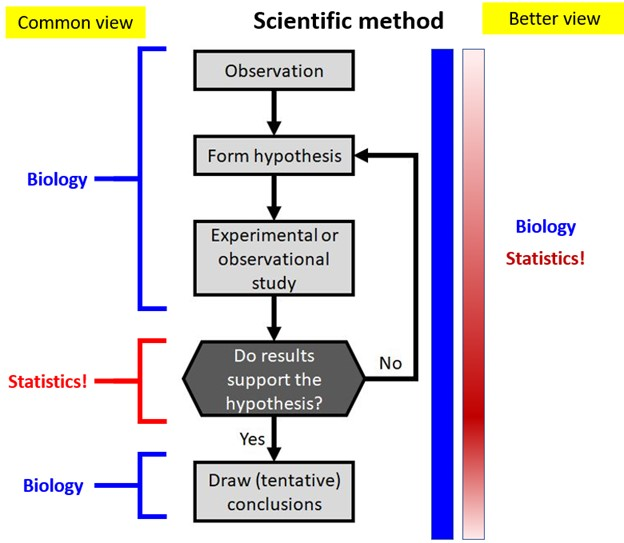
\includegraphics[keepaspectratio]{chapters/../images/01_01.jpg}}

}

\end{figure}%

So why do we, as biologists, need statistics? Some common answers might
include:

\begin{enumerate}
\def\labelenumi{\arabic{enumi}.}
\item
  ``To tell us whether the patterns we see in our data are real''
\item
  ``To tell whether the patterns in our data are due to chance or not.''
\item
  ``To prove our hypotheses.''
\end{enumerate}

All 3 of these are completely wrong. \textbf{1} is wrong because
confirming reality requires observation and experiment, not calculating.
\textbf{2} is a common misconception. \emph{Any} pattern in data could
be cause by chance. Statistics can help you estimate that probability,
but cannot tell you for sure. Finally, \textbf{3} is wrong because
that's not how science works. Hypotheses can be supported or not
supported. No amount of statistical analysis will ever completely rule
out chance.

So the answer to the question, ``Why do we as biologists need
statistics?'' is that we need a systematic way to determine whether data
support hypotheses are not. Note that I said ``systematic'', not
``absolutely correct''. As we will see shortly, statistical tests are
only a guide to decision-making. We should not fool ourselves into
thinking that our analyses are completely objective. Many aspects of the
analysis process are in fact \emph{subjective} and thus any analysis has
to be taken in its proper context, with caveats and biological reality
always in mind.

When we ``do statistics'', we are arguably not even answering biological
questions. Every statistical test answers a particular form of question:

\begin{itemize}
\item
  ``Do groups A and B have the same mean?''
\item
  ``As variable X changes, does variable Y tend to change?''
\item
  ``If variable X increases by this much, how much does variable Y
  change?''
\item
  ``If event G happens, how likely is it that event H also happens?''
\end{itemize}

Notice that these are ``statistical'' statements, not necessarily
biological statements. Translating biological ideas and questions into
statistical statements and questions is one of the hardest parts of
``doing statistics''.

\section{How do we use statistics in biology?}\label{sec-intro-tests}

Although there are hundreds, if not thousands, of statistical tests out
there, most biologists only ever need a handful. It turns out that
statistical hypotheses in biology tend to fall into just a few
categories:

\begin{enumerate}
\def\labelenumi{\arabic{enumi}.}
\item
  Testing for a \textbf{difference in mean or location} between groups.
\item
  Testing for a \textbf{continuous relationship} between a response
  variable (or multiple variables) and one or more predictor variables.
  Also referred to as \textbf{predicting} or \textbf{modeling} a
  continuous variable.
\item
  Testing for (lack of) \textbf{independence between categories} of
  observations.
\item
  Trying to \textbf{classify observations} based on predictor variables.
\end{enumerate}

These categories are not mutually exclusive, and many biological
questions can be phrased in more than one way. Understanding what kind
of pattern you looking for--that is, which of the 4 categories above
your question falls into--can get you a long way toward understanding
how to analyze your data.

\section{\texorpdfstring{\emph{P}-values and null
hypotheses}{P-values and null hypotheses}}\label{sec-intro-pvals}

\subsection{Null and alternative hypotheses}\label{sec-intro-pvals-null}

When scientists design experiments, they are testing one or more
hypotheses, or proposed explanations for a phenomenon. Contrary to
popular belief, the statistical analysis of experimental results usually
does not test a researcher's hypotheses directly. Instead, statistical
analysis of experimental results focuses on comparing experimental
results to the results that \emph{might have occurred} if there was no
effect of the factor under investigation.

In other words, traditional statistics sets up the following:

\begin{itemize}
\item
  \textbf{Null hypothesis or} \(H[0]\): default assumption that some
  effect (or quantity, or relationship, etc.) is zero and does not
  affect the experimental results.
\item
  \textbf{Alternative hypothesis or} \(H[a]\): assumption that the null
  hypothesis is false. Usually this is the researcher's scientific
  hypothesis, or proposed explanation for a phenomenon.
\end{itemize}

In (slightly) more concrete terms, if researchers want to test the
hypothesis that some factor \emph{X} has an effect on measurement
\emph{Y}, then they set up an experiment comparing observations of
\emph{Y} across different values of \emph{X}. They would then have the
following set up:

\begin{itemize}
\item
  \textbf{Null hypothesis:} Factor \emph{X} does not affect \emph{Y}.
\item
  \textbf{Alternative hypothesis:} Factor \emph{X} does affect \emph{Y}
\end{itemize}

Notice that in NHST the alternative hypothesis is the \textbf{logical
negation} of the null hypothesis, \textbf{\emph{not}} a statement about
another variable (e.g., ``Factor \emph{Z} affects \emph{Y}''). This is
an easy mistake to make and one of the weaknesses of NHST: the word
``hypothesis'' in the phrase ``null hypothesis'' is not being used in
the sense that scientists usually use it. This unfortunate choice of
vocabulary is responsible for generations of confusion among
researchers\footnote{Not to mention among generations of students taking
  statistics courses, myself included.}.

In order to test an ``alternative hypothesis'', what need is to
\emph{estimate} how likely the data would be if the null hypothesis were
true. If a pattern seen in the data is highly unlikely, this is taken as
evidence that the null hypothesis should be rejected in favor of the
alternative hypothesis. This is not the same as ``accepting'' or
``proving'' the alternative hypothesis.

The null hypothesis is usually translated to a prediction like one of
the following:

\begin{itemize}
\item
  The mean of \emph{Y} is the same for all levels of \emph{X}.
\item
  The mean of \emph{Y} does not differ between observations exposed to
  \emph{X} and observations not exposed to \emph{X}.
\item
  Outcome \emph{Y} is equally likely to occur when \emph{X} occurs as it
  is when \emph{X} does not occur.
\item
  Rank order of \emph{Y} values does not differ between levels of
  \emph{X}.
\end{itemize}

All of these predictions have something in common: \emph{Y} is
\textbf{independent} of \emph{X}. That's what the null hypothesis means.
To test the predictions of the null hypothesis, we need a way to
calculate what the data \emph{might have looked like if the null
hypothesis was correct}. Once we calculate that, we can compare the data
to those calculations to see how ``unlikely'' the actual data were. Data
that are sufficiently unlikely under the assumption that the null
hypothesis is correct---a ``significant difference''---are a kind of
evidence that the null hypothesis is false. If this sounds convoluted,
that's because it is.

This kind of analysis is referred to as \textbf{Null Hypothesis
Significance Testing (NHST)} and is one of the most important paradigms
in modern science. Whether or not this is a good thing is a subject of
fierce debate among scientists, statisticians, and philosophers of
science. For better or worse, NHST is all but the \emph{de facto}
standard of inference in scientific publishing, so regardless of its
merits in your particular case you will need to be able to use it. The
purpose of this course module is to encourage you to use it correctly.

The \emph{p}-value allows us to make binary distinctions, in a
systematic way, between situations where a null hypothesis is true and
no pattern is present, and situations where the null hypothesis is
highly unlikely to be true and thus a pattern might be present. Any
binary decision process has four possible outcomes:

\begin{enumerate}
\def\labelenumi{\arabic{enumi}.}
\tightlist
\item
  \textbf{True positive}: declare a pattern is present when it is
  present.
\item
  \textbf{True negative}: declare a pattern is absent, when it is
  absent.
\item
  \textbf{False positive}: declare a pattern is present, when it is
  actually absent. Also called a \textbf{Type I error}.
\item
  \textbf{False negative}: declare a pattern is absent, when it is
  actually present. Also called a \textbf{Type II error}.
\end{enumerate}

These outcomes can be summarized as shown below. Statisticians are
particularly concerned with the probabilities of false positives
(\(\alpha\)) and false negatives (\(\beta\)). The false positive
probability \(\alpha\) is the standard against which experimental
\emph{p}-values are compared. This is largely because we humans are
inordinately prone to finding patterns even when no patterns are
present--i.e., committing type I errors.

\begin{figure}[H]

\caption{Relationship between the null hypothesis and our decision about
experimental results. Type I and II errors result when we reject a true
null hypothesis and when we fail to reject a false null. The false
discovery rate, or Type I error rate, defined by \(\alpha\) is a very
important value in our approach to science.}

{\centering \pandocbounded{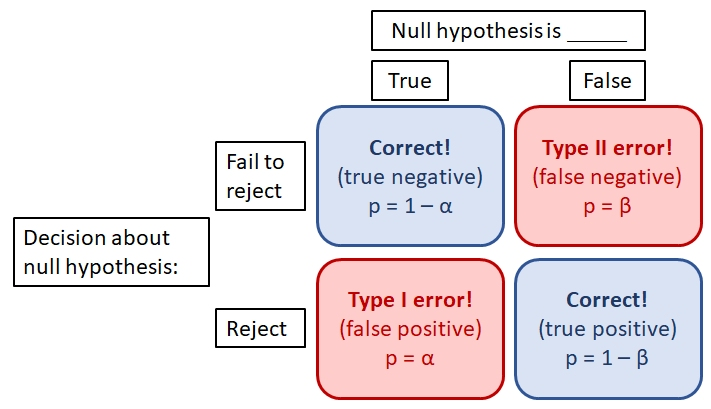
\includegraphics[keepaspectratio]{chapters/../images/01_02.jpg}}

}

\end{figure}%

Why have we evolved this way? Finding patterns in noisy data has helped
us discover virtually everything we know. So, pattern recognition must
be a powerful cognitive tool. But there is another interpretation, that
in our ancestral lifestyle life false positives were far less costly
than false negatives. Imagine you are an Australopithecine or an early
\emph{Homo erectus} (or \emph{H. sapiens}, for that matter), wandering
through the savanna of what will someday be modern Ethiopia, looking for
food. You hear a rustle in the tall grass a few meters ahead. Is that
rustle just the wind? Or is it a dangerous animal that will kill and
possibly eat you? Here are your choices and their consequences:

\begin{figure}[H]

\caption{Illustration of the consequences of Type I and Type II errors,
and why human minds may be so prone to Type I errors.}

{\centering \pandocbounded{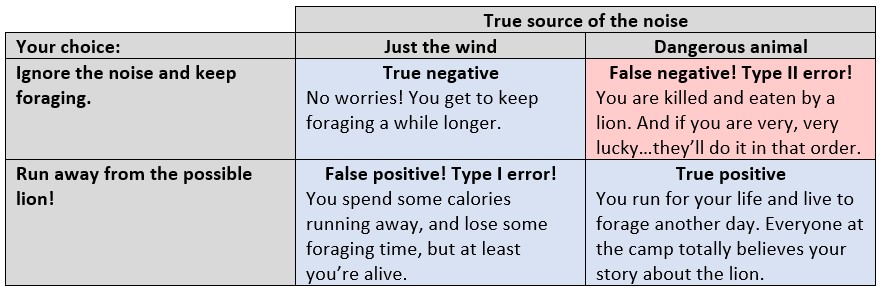
\includegraphics[keepaspectratio]{chapters/../images/01_03.jpg}}

}

\end{figure}%

Notice that of your choices, only the type II error has immediate
evolutionary consequences. In terms of fitness, the difference between a
type II error and a true positive (death vs.~survival) is much greater
than the difference between a true negative and a false positive (a bit
more food vs.~a mild inconvenience).

What does this have to do with statistics in biology? Our human minds
have evolved to find patterns in noisy data, and we are so good at it
that we frequently ``find'' patterns that aren't really there. So, we
use the scientific method and statistical analysis as tools to help
mitigate our bias toward pattern-finding.

\subsection{Another way to frame null
hypotheses}\label{sec-intro-pvals-alt}

When I teach statistics to biology majors, I try to avoid the terms
``null hypothesis'' and ``alternative hypothesis'' because most of my
students find them confusing. Instead, I ask students to ask two
questions about a hypothesis:

\begin{enumerate}
\def\labelenumi{\arabic{enumi}.}
\item
  What should we observe if the hypothesis \emph{is not} true?
\item
  What should we observe if the hypothesis \emph{is} true?
\end{enumerate}

In order to be \emph{scientific} hypothesis, both of those questions
have to be answerable. Otherwise, we have no way of distinguishing
between a situation where a hypothesis is supported, or a situation
where it is not, because experimental results could \emph{always} be due
to random chance (even if the probability of that is \emph{very} small).
All we can really do is estimate how likely it is that random chance
drove the outcome\footnote{You may have noticed that questions 1 and 2
  are really the null hypothesis and alternative hypothesis in disguise.}.

\subsection{\texorpdfstring{History and status of
\emph{p}-values}{History and status of p-values}}\label{sec-intro-pvals-hist}

The \emph{p}-value is a statistical statement about the likelihood of
observing a pattern in data when the null hypothesis is true. They were
first developed in the 1700s, and popularized by the statistician R.A.
Fisher in the 1920s. In Fisher's formulation, the \emph{p}-value was
only meant as a ``rule-of-thumb'' or \textbf{heuristic} for determining
whether the null hypothesis could be safely rejected. His original
publications did not imply that rejecting the null hypothesis should
automatically imply acceptance of the alternative hypothesis, or offer
any justification for particular cut-offs or critical values of
\emph{p}. Those ideas came later.

Fisher suggested a critical \emph{p}-value of 0.05 for convenience, but
did not prescribe its use. In fact, he also suggested using other
cut-offs, and even using the \emph{p}-value itself as a measure of
support for a hypothesis. The adoption of 0.05 as a threshold for
significance proved popular, and has been taken as a kind of gospel for
generations of researchers ever since.

In my opinion, the ubiquity of \emph{p}-values on scientific research
illustrates
\href{https://en.wikipedia.org/wiki/Goodhart\%27s_law}{Goodhart's Law}:
``When a measure becomes a target, it ceases to be a good measure''.
Because the cut-off value of \emph{p} \textless{} 0.05 is so widely used
and accepted as a measure of the ``truth'' of a hypothesis, many
researchers will take steps to ensure that their experiments produce
\emph{p}-values \textless{} 0.05. This can lead to the practices of
\emph{p}-hacking or data dredging. Or worse, setting up experiments to
test meaningless null hypotheses or analyzing data selectively.

The attention and effort spent increasing the likelihood of a
significant outcome is attention and effort that is not spent on
formulating hypotheses, developing theory, or conducting experiments.
Thus, intensive focus on \emph{p}-values can be a real distraction from
more important things.

These criticisms of \emph{p}-values are neither new nor little known.
Criticisms of the uncritical devotion to \emph{p}-values can be found
going back decades in the literature. In ecology, for example, debates
about the place of NHST flare up occasionally, as new advances in
statistical methods have offered opportunities for new inferential
paradigms.

Recently, the American Statistical Association (ASA) published a number
of papers criticizing the current use of \emph{p}-values and offering
alternatives. Wasserstein and Lazar (2016) provide a good starting point
to the series and an overview of the major themes. Some of the proposed
alternative or complementary methods have started to make their way into
various scientific disciplines. Others have not. By and large, NHST
remains the standard method of testing hypotheses with data and will
likely remain so for a long time.

\subsection{\texorpdfstring{Where \emph{p}-values come
from}{Where p-values come from}}\label{where-p-values-come-from}

So where do \emph{p}-values come from, anyway? Remember, \emph{p}-values
are an expression of how likely the observed data would be if the null
hypothesis was true. Then calculation of a \emph{p}-value involves
assumptions about the size of the effect (i.e., difference between the
results if the null is true vs.~not true), the variability of the
outcome (random or otherwise), and the distribution of different summary
statistics of the results assuming that the null hypothesis is true.
Let's consider the example of a \emph{t}-test. A \emph{t}-test is used
to compare means of two groups. We'll talk more about them in
\textbf{?@sec-groups-2ttest}. We will use R to simulate some data and
explore a basic \emph{t}-test.

\begin{Shaded}
\begin{Highlighting}[]
\FunctionTok{set.seed}\NormalTok{(}\DecValTok{123}\NormalTok{)}
\NormalTok{n }\OtherTok{\textless{}{-}} \DecValTok{10}
\NormalTok{mu1 }\OtherTok{\textless{}{-}} \DecValTok{6}
\NormalTok{mu2 }\OtherTok{\textless{}{-}} \DecValTok{8}
\NormalTok{sigma }\OtherTok{\textless{}{-}} \DecValTok{3}
\NormalTok{x1 }\OtherTok{\textless{}{-}} \FunctionTok{rnorm}\NormalTok{(n, mu1, sigma)}
\NormalTok{x2 }\OtherTok{\textless{}{-}} \FunctionTok{rnorm}\NormalTok{(n, mu2, sigma)}
\FunctionTok{t.test}\NormalTok{(x1, x2)}
\end{Highlighting}
\end{Shaded}

\begin{verbatim}

    Welch Two Sample t-test

data:  x1 and x2
t = -1.796, df = 17.872, p-value = 0.08941
alternative hypothesis: true difference in means is not equal to 0
95 percent confidence interval:
 -5.2131465  0.4091686
sample estimates:
mean of x mean of y 
 6.223877  8.625866 
\end{verbatim}

The results show us that the means of groups \texttt{x1} and \texttt{x2}
are not significantly different from each other (\emph{t} = -1.796,
17.87 d.f., \emph{p} = 0.0894). Because \emph{p} \(\ge\) 0.05, we cannot
reject the null hypothesis of no difference; i.e., the hypothesis that
the means of \texttt{x1} and \texttt{x2} are the same. This is
\textbf{\emph{not}} the same as concluding that the means are the same.
All we can say is that we cannot say the means are different.

But why? Where do the numbers in the output come from?

The \emph{t} value is what's called a \textbf{test statistic}. This is a
summary of the quantity of interest--difference in means--that depends
on the quantity of interest \emph{and} additional terms that describe
how that summary might vary randomly. In the case of the \emph{t}-test,
the test statistic \emph{t} is calculated as:

\[t=\frac{{\bar{x}}_1-{\bar{x}}_2}{\sqrt{\frac{s_1^2}{n_1}+\frac{s_2^2}{n_2}}}\]

In this equation:

\begin{itemize}
\tightlist
\item
  \({\bar{x}}_1\) and \({\bar{x}}_2\) are the means of two sets of
  values \(x_1\) and \(x_2\). A bar over a variable usually denotes a
  sample mean.
\item
  \(s_1^2\) and \(s_2^2\) are the sample variances of \(x_1\) and
  \(x_2\). The \textbf{variance} is a measure of how spread out values
  are away from the mean.
\item
  \(n_1\) and \(n_2\) are the number of observations in \(x_1\) and
  \(x_2\).
\end{itemize}

The numerator is the quantity we are interested in: the difference
between the means in group 1 and group 2. The denominator scales the
difference according to the sample size and the amount of variation in
both groups. Thus, \emph{t} accounts for the quantity of interest (the
pattern), the variability in the pattern, and the number of observations
of the pattern.

In the example above, the \emph{t} statistic was -1.796. This was the
difference in means (-2.402) scaled by the amount of random variation
(\(s_1^2\) and \(s_2^2\)) relative to the number of observations
(\(n_1\) and \(n_2\)). The ``significance'' of the test comes from the
fact that \emph{t}-statistics themselves follow a pattern called the
\textbf{Student's \emph{t} distribution}. The Student's \emph{t}
distribution describes how likely different values of \emph{t} are given
a certain sample size. This sample size used is not the total number of
observations, but instead a scaled version of sample size called
\textbf{degrees of freedom (d.f.)}. For the example above with 17.872
d.f., the \emph{t} distribution looks like this:

\begin{center}
\pandocbounded{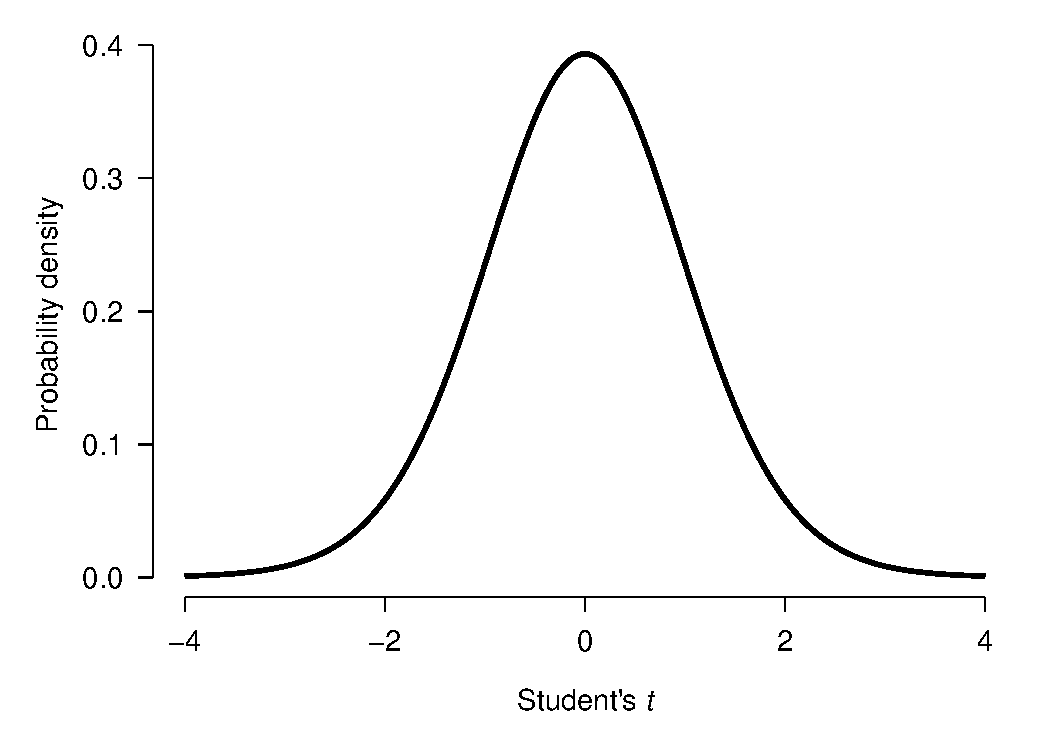
\includegraphics[keepaspectratio]{chapters/ch01_files/figure-pdf/unnamed-chunk-2-1.pdf}}
\end{center}

If there was no difference between the means of \texttt{x1} and
\texttt{x2}, then \emph{t} statistics of randomly generated datasets
should cluster around 0 with more extreme values being much less likely.
Test statistics \(\ge\) 4 or \(\le\) -4 almost never happen.

What about our \emph{t} statistic, -1.796? The figure below shows how
the total possible space of \emph{t} statistics (given 17.872 d.f.) is
partitioned. The total area under this curve, called a ``probability
density plot'', is equals 1. If you think about it, \emph{t} must take
on a value\ldots so the sum of probabilities for all t is 1. The red
area shows the probability of a \emph{t} occurring randomly that is
\(< -1.796\). That is, more extreme than the observed \emph{t}. But
``more extreme'' can work the other way too: \emph{t} could randomly be
\(> 1.796\) as well. This probability of this possibility is shown by
the blue area. The total of the red and blue areas is the total
probability of a \emph{t} value more extreme than the observed \emph{t}.

\begin{figure}[H]

\caption{The areas under the \emph{t} distribution probability density
curve outside the critical values of \emph{t} define the two-tailed
\emph{p}-value for the test.}

{\centering \pandocbounded{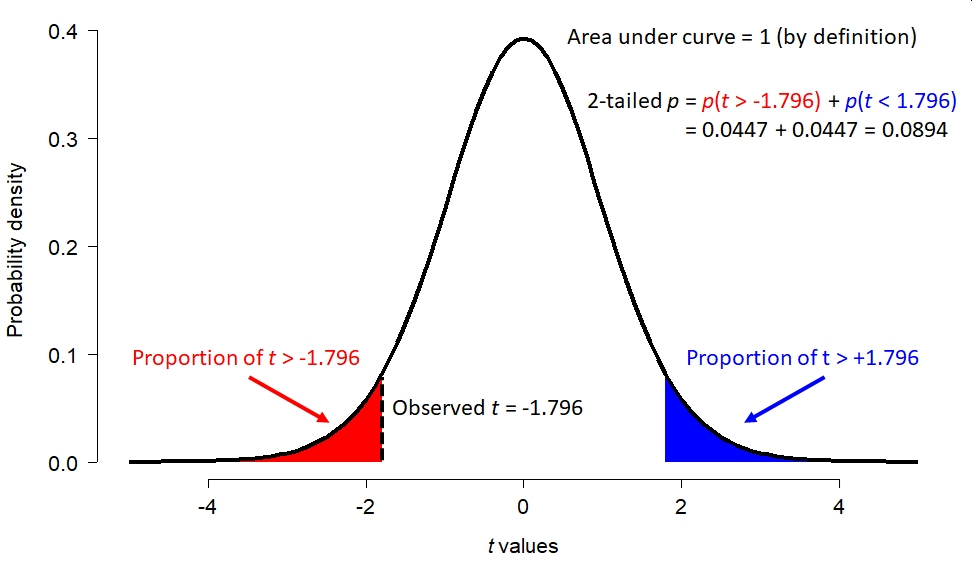
\includegraphics[keepaspectratio]{chapters/../images/01_04.jpg}}

}

\end{figure}%

But as we shall see, increasing the sample size can make the same
difference appear significant:

\begin{Shaded}
\begin{Highlighting}[]
\FunctionTok{set.seed}\NormalTok{(}\DecValTok{123}\NormalTok{)}
\NormalTok{n }\OtherTok{\textless{}{-}} \DecValTok{1000}
\NormalTok{mu1 }\OtherTok{\textless{}{-}} \DecValTok{6}
\NormalTok{mu2 }\OtherTok{\textless{}{-}} \DecValTok{8}
\NormalTok{sigma }\OtherTok{\textless{}{-}} \DecValTok{3}
\NormalTok{x1 }\OtherTok{\textless{}{-}} \FunctionTok{rnorm}\NormalTok{(n, mu1, sigma)}
\NormalTok{x2 }\OtherTok{\textless{}{-}} \FunctionTok{rnorm}\NormalTok{(n, mu2, sigma)}
\FunctionTok{t.test}\NormalTok{(x1, x2)}
\end{Highlighting}
\end{Shaded}

\begin{verbatim}

    Welch Two Sample t-test

data:  x1 and x2
t = -15.485, df = 1997.4, p-value < 2.2e-16
alternative hypothesis: true difference in means is not equal to 0
95 percent confidence interval:
 -2.342319 -1.815705
sample estimates:
mean of x mean of y 
 6.048384  8.127396 
\end{verbatim}

We can also find a significant \emph{p}-value by reducing the amount of
variation (\texttt{sigma}, or \(\sigma\)). In this example, variance
within each group is expressed as the residual standard deviation (SD).
\textbf{Residual} variation is variation not explained by the model
(i.e., not related to the difference in means between groups). The SD is
the square root of the variance, and is how R expresses the variation in
a normal distribution (\texttt{rnorm()}).

\begin{Shaded}
\begin{Highlighting}[]
\FunctionTok{set.seed}\NormalTok{(}\DecValTok{123}\NormalTok{)}
\NormalTok{n }\OtherTok{\textless{}{-}} \DecValTok{10}
\NormalTok{mu1 }\OtherTok{\textless{}{-}} \DecValTok{6}
\NormalTok{mu2 }\OtherTok{\textless{}{-}} \DecValTok{8}
\NormalTok{sigma }\OtherTok{\textless{}{-}} \FloatTok{0.001}
\NormalTok{x1 }\OtherTok{\textless{}{-}} \FunctionTok{rnorm}\NormalTok{(n, mu1, sigma)}
\NormalTok{x2 }\OtherTok{\textless{}{-}} \FunctionTok{rnorm}\NormalTok{(n, mu2, sigma)}
\FunctionTok{t.test}\NormalTok{(x1, x2)}
\end{Highlighting}
\end{Shaded}

\begin{verbatim}

    Welch Two Sample t-test

data:  x1 and x2
t = -4486.7, df = 17.872, p-value < 2.2e-16
alternative hypothesis: true difference in means is not equal to 0
95 percent confidence interval:
 -2.001071 -1.999197
sample estimates:
mean of x mean of y 
 6.000075  8.000209 
\end{verbatim}

So, what the \emph{P}-value in our \emph{t}-test tells us depends on not
just the actual difference, but how variable that difference is and how
many times we measure it.

The table below summarizes the results of the three simulations we just
ran:

{\def\LTcaptype{none} % do not increment counter
\begin{longtable}[]{@{}
  >{\raggedright\arraybackslash}p{(\linewidth - 8\tabcolsep) * \real{0.2000}}
  >{\raggedleft\arraybackslash}p{(\linewidth - 8\tabcolsep) * \real{0.2000}}
  >{\raggedleft\arraybackslash}p{(\linewidth - 8\tabcolsep) * \real{0.2000}}
  >{\raggedleft\arraybackslash}p{(\linewidth - 8\tabcolsep) * \real{0.2000}}
  >{\centering\arraybackslash}p{(\linewidth - 8\tabcolsep) * \real{0.2000}}@{}}
\toprule\noalign{}
\begin{minipage}[b]{\linewidth}\raggedright
True difference (\({\bar{x}}_1-{\bar{x}}_2\))
\end{minipage} & \begin{minipage}[b]{\linewidth}\raggedleft
Residual SD
\end{minipage} & \begin{minipage}[b]{\linewidth}\raggedleft
Sample size
\end{minipage} & \begin{minipage}[b]{\linewidth}\raggedleft
\emph{p}-value
\end{minipage} & \begin{minipage}[b]{\linewidth}\centering
Significant?
\end{minipage} \\
\midrule\noalign{}
\endhead
\bottomrule\noalign{}
\endlastfoot
-2 & 3 & 20 & 0.089 & No \\
-2 & 3 & 2000 & \(<0.001\) & Yes \\
-2 & 0.001 & 20 & \(<0.001\) & Yes \\
\end{longtable}
}

\subsection{\texorpdfstring{What \emph{p}-values mean and do not
mean}{What p-values mean and do not mean}}\label{what-p-values-mean-and-do-not-mean}

In the simulations above, we know that the true difference was -2
because that is how we generated the numbers. But the conclusion of the
experiments depended on experimental parameters other than the one of
interest! For each of the three scenarios above, consider these
questions:

\begin{itemize}
\tightlist
\item
  Should the researchers reject the null hypothesis, and conclude that
  there is a difference between \texttt{x1} and \texttt{x2}?
\item
  Should the researchers accept the null hypothesis, and conclude that
  there is no difference between \texttt{x1} and \texttt{x2}?
\item
  Should the researchers accept the alternative hypothesis, and conclude
  that there is a difference between \texttt{x1} and \texttt{x2}?
\end{itemize}

The researchers should reject the null hypothesis only in scenarios 2
and 3. In scenario 1, they should not ``accept'' the null hypothesis.
The correct action is \textbf{fail to reject} the null. Accepting the
null hypothesis would imply some certainty that the difference was 0.
But that is not what the \emph{t}-test actually says. What the
\emph{t}-test really says is that a difference (measured as \emph{t})
between -1.796 and 1.796 is likely to occur about 91\% (i.e.,
1-\emph{P}) of the time even if the true difference is 0. In other
words, if we repeated the experiment, we would get a \(|t|>1.796\) over
9 times out of 10!

One of the most common misconceptions about \emph{p}-values is that they
represent the probability of the null hypothesis being true, or of the
alternative hypothesis being false. \textbf{Neither of these
interpretations is correct.} Similarly, many people think that 1 minus
the \emph{p}-value represents the probability that the alternative
hypothesis is true. This is also incorrect.

Remember:

\begin{itemize}
\tightlist
\item
  The \emph{p}-value is only a statistical summary, and says nothing
  about whether or not a hypothesis is true.
\item
  The \emph{p}-value is only a statement about how unlikely the result
  would be if there was no real effect.
\item
  A \emph{p}-value is a purely statistical calculation and says nothing
  about biological importance or the truth of your hypothesis.
\item
  Interpreting \emph{p}-values and other statistical outputs is the job
  of the scientist, not the computer.
\end{itemize}

If it feels like I'm belaboring these points, it's because I am. The
\emph{p}-value and NHST in general are merely a set of heuristics to
help researchers make binary distinctions like:

\begin{itemize}
\tightlist
\item
  Reject \textbf{\emph{or}} fail to reject the null hypothesis.
\item
  True difference is 0 \textbf{\emph{or}} not 0.
\item
  Difference is \(\ge3\) \textbf{\emph{or}} not \(<3\).
\item
  And so on.
\end{itemize}

These distinctions are binary because each condition is the logical
negation of the other. But, \emph{rejecting} one side of each dichotomy
is \emph{not the same as accepting} the other. By analogy, juries in
criminal trials in the USA make one of two determinations: guilty or not
guilty. A verdict of not guilty includes innocent as a possibility, but
does not necessarily mean that the jury thinks the defendant is
innocent. It simply means that the jury does not feel that the defendant
has been \emph{proven} guilty.

Likewise, the \emph{p}-value might help distinguish ``difference in
means is different from 0 (\(p<0.05\))'' vs.~``difference in means is
not different from 0 (\(p\ge0.05\))''. The latter choice includes a
difference in means of 0 as a possibility, but does not actually
demonstrate that the value is 0.

\subsection{\texorpdfstring{Do you need a
\emph{p}-value?}{Do you need a p-value?}}\label{do-you-need-a-p-value}

Now that we have a better handle on what a \emph{p}-value really is, you
might be tempted to ask, ``Do I need a \emph{p}-value?'' Yes, you
probably do. For better or for worse, \emph{p}-values and NHST are
firmly entrenched in most areas of science, including biology. Despite
its shortcomings, the NHST paradigm does offer a powerful way to test
and reject proposed explanations. This utility means that NHST and
\emph{p}-values are not going away any time soon. If you want an
alternative to \emph{p-}values and NHST, refer to Chapter~\ref{sec-it}
or Chapter~\ref{sec-bayes}.

\part{Introduction to R}

Why. Doesn't. It. Work?

\chapter{Introduction to R}\label{sec-r}

This module is an introduction to the R program and language. We will
begin with downloading and installing R, then explore the basics of
running R commands and storing data, and finally answer some frequently
asked questions (FAQ). Some of the topics in this module are covered in
greater detail in Chapter~\ref{sec-object}, Chapter~\ref{sec-ie}, and
Chapter~\ref{sec-manip}. The current module is meant to get you up and
running before moving on to more advanced material.

By the end of this module you should be able to:

\begin{itemize}
\tightlist
\item
  Explain what R is and what it is used for
\item
  Explain the object-oriented programming paradigm used by R
\item
  Download and install R and RStudio
\item
  Write and execute commands in the R console
\item
  Describe basic R data types and structures
\item
  Manage R code as scripts (.r files)
\item
  Manage and use R packages
\item
  Identify sources of help for R programming
\end{itemize}

\section{Getting started with R}\label{sec-r-start}

\subsection{Download and install R (and
RStudio)}\label{sec-r-start-install}

If you are on a university campus, many on-campus computers may already
have R installed on them. This is the bare minimum you need to work with
R. Many people also prefer to use another program for writing R code.
The most popular is probably \href{https://posit.co/downloads}{RStudio},
which is a more user-friendly interface for R. If you are on a PC or
Mac, you will need to download and install both R and RStudio. If you
are using a Linux machine, you may already have R because it is included
in some distros. You can still install RStudio to make your life easier.

First, install the latest version of R from the
\href{https://cran.r-project.org/mirrors.html}{R-project website}
(accessed 2021-12-20). Select a mirror (download server) from the list.
Once you select a mirror, you will be taken to a page where you will
select the version of R that corresponds to your operating system. Click
on the appropriate link for your operating system and follow the
instructions from there to install R. Like many programs you download
from the internet, R will come with an installer that will largely take
care of everything automatically. Just let the installer run and accept
the default options.

Next, install any code editing or IDE you want.

\begin{itemize}
\item
  RStudio can be installed from \href{https://posit.co/downloads/}{here}
  (accessed 2025-08-06). Select the version that corresponds to your
  operating system. As you did when you installed R, just let the
  installer run and accept the default options.
\item
  My personal favorite is Notepad++, which isn't an IDE but instead a
  very feature-rich code editor.
\item
  Other popular choices include
  \href{https://code.visualstudio.com/download}{Visual Studio Code} and
  \href{https://www.gnu.org/software/emacs/}{emacs}.
\end{itemize}

\subsection{Using R}\label{sec-r-start-using}

\subsubsection{Base R GUI}\label{base-r-gui}

R has a very basic front end, or \textbf{graphical user interface
(GUI)}. Most users find it easier to write their R code in another
program. Some of these programs, such as RStudio, are \textbf{integrated
development environments (IDE)}. Others are text editors with
programming capabilities. We'll explore the default R GUI first and then
meet some editor options. The basic R GUI is shown below. Your screen
may look different than mine because I set some graphics options.

\begin{figure}[H]

\caption{The base R GUI. Some like it (I do) but it's not for everyone.}

{\centering \pandocbounded{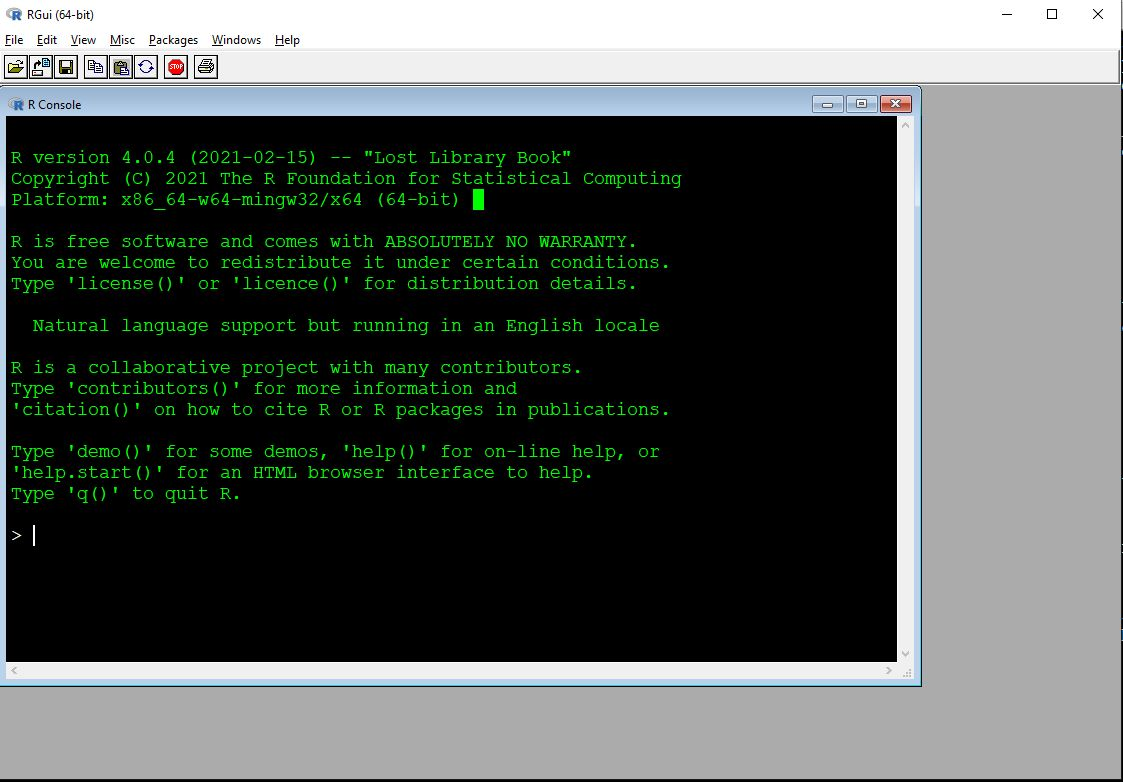
\includegraphics[keepaspectratio]{chapters/../images/02_01.jpg}}

}

\end{figure}%

The main window with R is the \textbf{R console}. This is the command
line interface to R. Some important features of the console are:

\begin{enumerate}
\def\labelenumi{\arabic{enumi}.}
\item
  Command prompt: The \texttt{\textgreater{}} symbol signifies the
  beginning of a command. You can enter commands here.
\item
  Continue prompt: \texttt{+} signifies the continuation of a previous
  command. If you have a \texttt{+} at the beginning of your line, you
  can get back to a new line using ESCAPE. Note that this will delete
  the currently incomplete line or command.
\item
  The ENTER key executes the current command. This could mean the
  current line, or multiple lines going back to the most recent
  \texttt{\textgreater{}}.
\item
  \texttt{{[}1{]}} at the beginning of results: because your result is
  an object (with length \(\ge\) 1). The very first value (``element'')
  in the result is element 1.
\item
  Up arrow key: cycles through previously entered commands. You can see
  many previous commands at once by using the command
  \texttt{history()}.
\end{enumerate}

Other important features of the R GUI are found in the menu bar:

\begin{itemize}
\tightlist
\item
  \textbf{File}

  \begin{itemize}
  \tightlist
  \item
    \textbf{New script}: opens a new script window within the GUI.
  \item
    Ability to open saved scripts or load previous workspaces
  \end{itemize}
\item
  \textbf{Edit}

  \begin{itemize}
  \tightlist
  \item
    \textbf{Copy, paste, etc.}: very useful!
  \item
    \textbf{Data editor}: opens a rudimentary spreadsheet-like viewer
    for datasets that can be used to make edits. Not recommended for
    routine use.
  \item
    \textbf{GUI preferences}: options to change colors, fonts, font
    sizes, etc., in the GUI. To make changes permanent you will need to
    save a new \texttt{.RConsole} file in your home directory.
  \end{itemize}
\item
  \textbf{View}
\item
  \textbf{Misc}

  \begin{itemize}
  \tightlist
  \item
    \textbf{List objects}: lists all objects in workspace. Equivalent to
    command \texttt{ls()}.
  \item
    \textbf{Remove all objects}: removes all objects form workspace.
    Equivalent to command \texttt{rm(list=ls(all=TRUE))}.
  \item
    \textbf{List search path}: lists currently attached packages.
    Equivalent to command \texttt{search()}.
  \end{itemize}
\item
  \textbf{Packages}: functions to download and install packages.
\item
  \textbf{Windows}: options to change how windows are displayed within
  GUI.
\item
  \textbf{Help}: options and resources for getting help, including
  several free R manuals in PDF format.
\end{itemize}

\subsubsection{Using R in RStudio}\label{using-r-in-rstudio}

Although you can type R code directly into the console, or type in
script windows within the base R GUI, it is usually easiest to use a
separate program for writing code. The two best, in my experience, are
RStudio and Notepad++ (see above). \textbf{RStudio} is an IDE designed
to manage R projects, and has many useful features. Unlike some other
options, RStudio has R built in so you can write code and execute it
within the same program. RStudio can be used on Windows, Mac, and Linux
operating systems. RStudio also has built-in support for utilities like
RMarkdown and Quarto (which was used to build this website).

Once you have RStudio installed, open it and you will see a screen like
this:

\begin{figure}[H]

\caption{The default RStudio set up, with some graphics options set for
dark mode.}

{\centering \pandocbounded{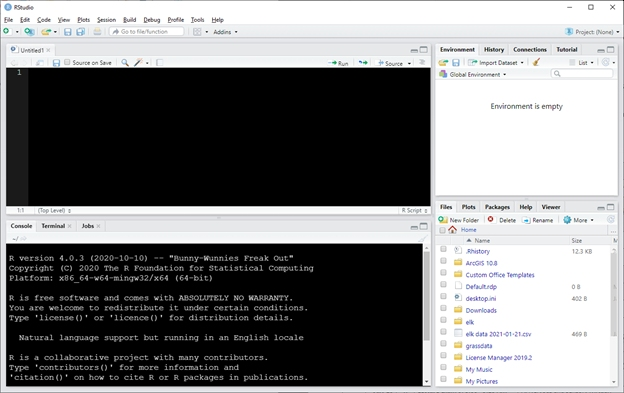
\includegraphics[keepaspectratio]{chapters/../images/02_02.jpg}}

}

\end{figure}%

Your RStudio might look different at first. You can change the color
scheme by going to Tools - Global Options - Appearance and selecting a
theme. Here I'm using the ``Classic'' theme with size 12 Courier New
font and 110\% zoom.

RStudio has an entire environment for working with R in one window. Each
of the panels performs different functions. Starting at the bottom left
and going clockwise, the panels are:

\begin{itemize}
\tightlist
\item
  \textbf{Console}: command line interface for R. You can type commands
  here and execute them by pressing ENTER.
\item
  \textbf{Script}: a space where you can type code and later execute it
  by either clicking ``Run'' or pressing CRTL-ENTER (CMD-ENTER on a
  Mac). Usually people write code in the script window rather than
  typing it directly into the console.
\item
  \textbf{Environment}: this window lists all of the data objects that
  you have loaded.
\item
  \textbf{Files}: this window lists all of the files available in your R
  home directory. You can also navigate to other folders on your machine
  and select files to open.
\end{itemize}

The bottom right panel also has a tab called ``\textbf{Plots}''. This is
where plots that you make can be seen. Sometimes you will need to resize
this panel to see the plots clearly. All of the panels can be resized by
clicking and dragging the borders between them.

\section{Commands, objects, and output}\label{sec-r-comm}

The key to understanding R is to understand
\href{https://en.wikipedia.org/wiki/Object-oriented_programming}{object
orientation}. This means that R code is built around manipulating
objects. In programming, an \textbf{object} is a construct or thing with
well-defined attributes and behaviors. For example, a graphics program
might have object classes like ``polygon'' and ``circle''. Rather than
redefine ``polygon'' every time the user needs to draw a polygon, the
program creates a polygon object with attributes like ``number of
sides'' and ``side length''. The new object is an \textbf{instance} of
the polygon class. The \textbf{class} of an object defines what
attributes it has and how it interacts with other objects.

\subsection{R commands--basics}\label{sec-r-comm-basic}

In R, \textbf{\emph{everything}} is an object. We will learn more about
some of the most important R object types in the examples in
Chapter~\ref{sec-object}. Objects are created in R by many functions.

Objects are stored to memory by \textbf{assignment}, using the left
arrow \texttt{\textless{}-} (a ``less than'' followed by a hyphen). If
an object already exists, then assignment is used to either modify the
object, or replace it entirely. Here is an example:

\begin{Shaded}
\begin{Highlighting}[]
\NormalTok{a }\OtherTok{\textless{}{-}} \DecValTok{3}
\end{Highlighting}
\end{Shaded}

This creates an object called \texttt{a}, which contains the value
\texttt{3}. You can then recall the value by typing \texttt{a} in the
console and pressing Enter. You can also use the value stored in
\texttt{a} in calculations or functions.

\begin{Shaded}
\begin{Highlighting}[]
\NormalTok{a}
\end{Highlighting}
\end{Shaded}

\begin{verbatim}
[1] 3
\end{verbatim}

\begin{Shaded}
\begin{Highlighting}[]
\NormalTok{a }\SpecialCharTok{*} \DecValTok{2}
\end{Highlighting}
\end{Shaded}

\begin{verbatim}
[1] 6
\end{verbatim}

\begin{Shaded}
\begin{Highlighting}[]
\DecValTok{1}\SpecialCharTok{:}\NormalTok{a}
\end{Highlighting}
\end{Shaded}

\begin{verbatim}
[1] 1 2 3
\end{verbatim}

Assigning a different value to \texttt{a} will overwrite it.

\begin{Shaded}
\begin{Highlighting}[]
\NormalTok{a}
\end{Highlighting}
\end{Shaded}

\begin{verbatim}
[1] 3
\end{verbatim}

\begin{Shaded}
\begin{Highlighting}[]
\NormalTok{a }\OtherTok{\textless{}{-}} \DecValTok{6}
\NormalTok{a}
\end{Highlighting}
\end{Shaded}

\begin{verbatim}
[1] 6
\end{verbatim}

\begin{Shaded}
\begin{Highlighting}[]
\NormalTok{a}\SpecialCharTok{\^{}}\DecValTok{2}
\end{Highlighting}
\end{Shaded}

\begin{verbatim}
[1] 36
\end{verbatim}

Notice that there is no ``Undo'' button. If you make a mistake, you need
to rerun the code before your mistake to get back to where you were.
Objects can be deleted by ``removing them'' with command \texttt{rm()}.

\begin{Shaded}
\begin{Highlighting}[]
\FunctionTok{rm}\NormalTok{(a)}
\end{Highlighting}
\end{Shaded}

Besides assigning and working with values, R code contains comments:
text that is for human readers, and is not interpreted by R. Comments
are very important because they tell other people---or future you---what
your code is doing and how it works. Some comments are just place
markers (e.g., \texttt{\#\ Analysis\ begins\ here}) to help you find
important sections. Other comments might be more lengthy, holding
explanations of why you chose to code a task the way that you did (e.g.,
\texttt{\#\ condense\ with\ sapply()\ (maintains\ order\ of\ subunits)}).
The latter kind of comment can be very useful to your future self.

In R, comments are made with the \# symbol. Anything on a line after \#
is not read by R.

\begin{Shaded}
\begin{Highlighting}[]
\CommentTok{\# here is a comment}
\NormalTok{b }\OtherTok{\textless{}{-}} \DecValTok{5} \CommentTok{\# here is another comment}
\end{Highlighting}
\end{Shaded}

You can write your code directly in the console, or in a script window.
If you use the script panel in RStudio (as you should), you can send
commands to the console by pressing Crtl-Enter (or Cmd-Enter on Mac).
This will send and execute the entire command that the cursor is on. In
the base R GUI script window, the equivalent is Crtl-R (or Cmd-R on
Mac), but this runs only the line where the cursor rests (not the entire
command).

The R console can seem daunting to new users. The
\texttt{\textgreater{}} symbol at the start of a line is the
\textbf{command prompt}. Commands must begin here. If there is a
\texttt{+} at the beginning of a line, then this means that there is an
incomplete command. Press Escape to exit the incomplete command and get
back to \texttt{\textgreater{}}.

When you type a command like \texttt{2+2}, the output will print to the
console with a \texttt{{[}1{]}} at the start of the line. The
\texttt{{[}1{]}} signifies that that line starts with the first element
of the output. This is to help read outputs with lots of elements. Try
the command \texttt{rnorm(100)} to see why.

\begin{Shaded}
\begin{Highlighting}[]
\DecValTok{2}\SpecialCharTok{+}\DecValTok{2}
\end{Highlighting}
\end{Shaded}

\begin{verbatim}
[1] 4
\end{verbatim}

\begin{Shaded}
\begin{Highlighting}[]
\FunctionTok{rnorm}\NormalTok{(}\DecValTok{100}\NormalTok{)}
\end{Highlighting}
\end{Shaded}

\begin{verbatim}
  [1] -1.600748770 -0.266624052 -0.637836355  0.993755884  2.598512518
  [6]  2.058009415  0.582003185 -1.367702261 -1.316874217 -0.135171516
 [11] -0.166490940  0.407665140  0.858663531 -0.323472514  0.988322630
 [16] -1.277271909  1.686499999  2.215667155 -0.126782716  1.103479887
 [21]  0.381607537 -0.544989714 -1.425527683 -0.515057798  0.196673515
 [26]  0.329542049  2.169272010  0.145446814 -0.606075762  0.702418529
 [31] -0.461643814 -0.429090193  0.116904022  0.436272406 -0.784784033
 [36]  1.147497864  0.326705501  0.962396682 -2.386840343  0.520445695
 [41] -0.513326419  0.607515614  1.932085554  2.387268675 -0.843865384
 [46]  0.643713128 -0.944476207 -0.878426853 -0.355530996  1.002566525
 [51] -0.025234993  0.758019117  1.765445578  1.033315126 -0.582001786
 [56]  0.230750581  1.252366722 -0.250633391 -0.866463805  0.363897402
 [61] -0.069641463  0.001439344  0.297169561 -1.103626198 -1.553981027
 [66] -0.158958867 -0.986857363  1.387334985 -1.773075370 -1.455899167
 [71] -1.612458825  0.621948653  0.878261109 -0.048466277  0.148077358
 [76] -0.986319636 -0.253009168  1.330801369  0.761788954 -0.502555398
 [81]  1.598215488 -1.356784839 -0.150874333  0.724587833  0.994102009
 [86] -2.306341308 -0.681825906  1.586009695  0.804039268 -0.162220599
 [91] -0.008568770  0.013186966 -0.274324348 -0.027369891  0.189356166
 [96] -1.291232463  0.403872013 -0.908246452  0.417759657 -0.824080472
\end{verbatim}

Commands can be split over multiple lines. When that happens, a
\texttt{+} will be seen at the left side of the window instead of a
\texttt{\textgreater{}}. A split command will be executed once a
complete expression is input.

If you accidentally start a command and aren't sure how to finish it,
you can exit and cancel the command with the ESCAPE key. R executes
commands, not lines. You can have more than one command on a line
separated by a semi-colon ;, but this generally frowned upon.

\begin{Shaded}
\begin{Highlighting}[]
\CommentTok{\# command split across lines:}
\DecValTok{2} \SpecialCharTok{+} 
\DecValTok{1}
\end{Highlighting}
\end{Shaded}

\begin{verbatim}
[1] 3
\end{verbatim}

\begin{Shaded}
\begin{Highlighting}[]
\CommentTok{\# 2 commands on a line (don\textquotesingle{}t do this)}
\DecValTok{2} \SpecialCharTok{+} \DecValTok{2}\NormalTok{; }\DecValTok{3} \SpecialCharTok{+} \DecValTok{3}
\end{Highlighting}
\end{Shaded}

\begin{verbatim}
[1] 4
\end{verbatim}

\begin{verbatim}
[1] 6
\end{verbatim}

Below is an example where the a command is broken across lines, with
each line getting an explanatory comment. This is possible because R
ignores whitespace (spaces, tabs, returns, etc.). Very complex functions
or loops might benefit from this kind of commenting. Some programmers do
not like this kind of comment--but you comment code the way that works
for you.

\begin{Shaded}
\begin{Highlighting}[]
\FunctionTok{rnorm}\NormalTok{(}
  \DecValTok{10}\NormalTok{,  }\CommentTok{\# sample size}
  \DecValTok{10}\NormalTok{,  }\CommentTok{\# mean}
  \DecValTok{2}    \CommentTok{\# sd}
       \CommentTok{\# note no comma after last argument!}
\NormalTok{)}\CommentTok{\#rnorm}
\end{Highlighting}
\end{Shaded}

\begin{verbatim}
 [1]  9.310467  9.976210  8.021102  8.521752  9.977428  8.567394
 [7]  7.153071  9.137187 14.897596 10.804013
\end{verbatim}

Notice in the above example that the closing parenthesis for
\texttt{rnorm()} is marked with a comment. This is a good practice if
the open and close parentheses are separated by many lines of code. Most
IDEs will highlight matching parentheses, but marking them yourself can
potentially save some headache.

When writing comments or writing multi-line commands you should keep in
mind that most code editors don't do line breaks very well. Or, they
will wrap text displayed in the editor, but this might not display the
same on every device. As a rule I try to keep lines of code to ≤ 80
characters, so I don't have to scroll over to see the end of a command.
You can do this too, by breaking up commands and long comments into
multiple lines. It also helps to indent additional lines by a set
amount--most people prefer either 2 or 4 spaces rather than a tab stop.

\subsection{Using R functions}\label{sec-r-comm-functions}

R \textbf{functions} are objects that do things to other objects, or
create objects, or modify objects\ldots{} basically, functions
\textbf{\emph{do}} stuff while most other objects \textbf{\emph{store}}
stuff. Functions are called by name, and they have options or
\textbf{arguments} contained within parentheses. It's good practice to
have the parentheses touching the function name.

Argument values are set using single equals sign \texttt{=}. Argument
values must be of the correct \textbf{type} (numeric, character,
logical, etc.), must take on valid values (or be one of the available
options), must be spelled and capitalized correctly, and may be named or
not at the user's discretion. Most functions will print their results to
the console upon completion. If you want to store the results of a
function, you need to assign the results to an object using
\texttt{\textless{}-}.

\begin{figure}[H]

\caption{Basic structure of an R command and its arguments.}

{\centering \pandocbounded{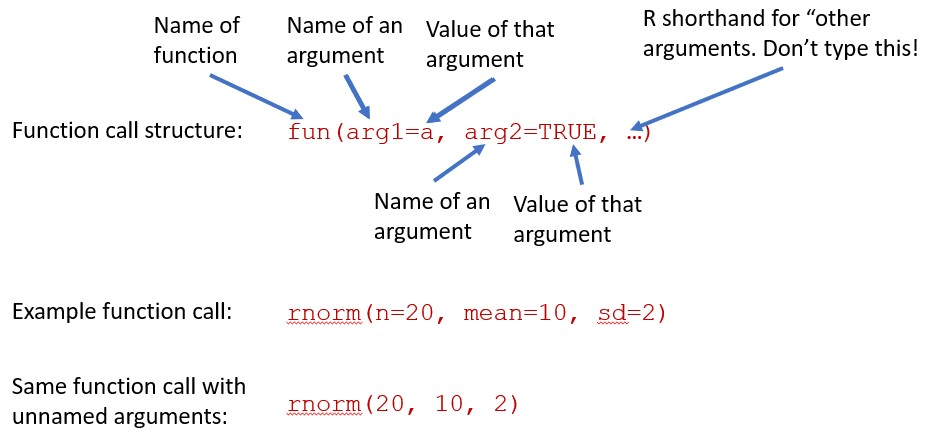
\includegraphics[keepaspectratio]{chapters/../images/02_04.jpg}}

}

\end{figure}%

See below for some examples of function use using \texttt{rnorm()},
which draws random numbers from a normal distribution\footnote{The
  normal distribution comes up a lot in statistics. It is sometimes
  called the ``bell curve'', but this is inappropriate because many
  distributions can be bell-shaped. It is also called the ``Gaussian''
  distribution, but Gauss did not discover it. The normal distribution
  is defined by its mean \(\mu\) and its standard deviation (SD)
  \(\sigma\). In other words, its central tendency and spread,
  respectively.}. Your numbers may be different than those below,
because the function is \emph{random}.

\begin{Shaded}
\begin{Highlighting}[]
\CommentTok{\# arguments named}
\DocumentationTok{\#\# draw 20 values with mean 10 and sd 2}
\FunctionTok{rnorm}\NormalTok{(}\AttributeTok{n=}\DecValTok{20}\NormalTok{, }\AttributeTok{mean=}\DecValTok{10}\NormalTok{, }\AttributeTok{sd=}\DecValTok{2}\NormalTok{)}
\end{Highlighting}
\end{Shaded}

\begin{verbatim}
 [1] 10.927458 12.232584  8.908545 10.806007 13.614292 10.260973
 [7] 12.176472 10.659363  6.012465  9.888794  8.596251 10.776733
[13] 10.391948  9.115058  9.396709 12.699707 10.028287  9.493144
[19] 13.345148  8.331533
\end{verbatim}

\begin{Shaded}
\begin{Highlighting}[]
\DocumentationTok{\#\# equivalent with unnamed arguments}
\FunctionTok{rnorm}\NormalTok{(}\DecValTok{20}\NormalTok{, }\DecValTok{10}\NormalTok{, }\DecValTok{2}\NormalTok{)}
\end{Highlighting}
\end{Shaded}

\begin{verbatim}
 [1] 11.277675 10.488317  9.087422  6.232064  6.709863 10.092402
 [7] 13.254079  9.526039  9.224622 10.545279  7.998203 12.479325
[13] 10.905517  7.357862 12.189891 11.475283 11.527040 11.623623
[19]  9.673827  7.925945
\end{verbatim}

\begin{Shaded}
\begin{Highlighting}[]
\DocumentationTok{\#\# very different: 2 values from a normal}
\DocumentationTok{\#\# distribution with mean=20 and sd=10}
\FunctionTok{rnorm}\NormalTok{(}\DecValTok{2}\NormalTok{, }\DecValTok{20}\NormalTok{, }\DecValTok{10}\NormalTok{)}
\end{Highlighting}
\end{Shaded}

\begin{verbatim}
[1] 17.45336 33.53970
\end{verbatim}

\begin{Shaded}
\begin{Highlighting}[]
\DocumentationTok{\#\# when in doubt, name your arguments!}
\FunctionTok{rnorm}\NormalTok{(}\AttributeTok{sd=}\DecValTok{2}\NormalTok{, }\AttributeTok{n=}\DecValTok{20}\NormalTok{, }\AttributeTok{mean=}\DecValTok{10}\NormalTok{)}
\end{Highlighting}
\end{Shaded}

\begin{verbatim}
 [1] 11.760061  7.494362 13.276145  9.814387 15.109935 11.155125
 [7] 10.200439  8.436808 10.244158  6.132275 10.079200 10.971345
[13] 11.457399  8.147205  7.040388 13.902765  9.988014  9.660902
[19] 12.001616 10.544832
\end{verbatim}

You can use the R help pages to see what the arguments are, the order in
which R expects them, and their default values (if any). For
\texttt{rnorm()}, the mean and sd have defaults 0 and 1, respectively.

\begin{Shaded}
\begin{Highlighting}[]
\NormalTok{?rnorm}
\end{Highlighting}
\end{Shaded}

To recap, argument \textbf{order} is important when using functions. You
can supply arguments to a function without naming them if you put them
in the proper order. See the help files to see what the order is.
\emph{When in doubt, name your arguments}.

Functions expect arguments in a particular format. If a function is not
working, you might have an argument formatted incorrectly. Sometimes
it's helpful to look at each argument separately in the R console,
outside of the function. To do this, copy/paste each argument to the R
console separately and execute by hitting ENTER.

Some function arguments have default values, so you don't have to supply
them. For example, \texttt{runif()}, which draws random numbers from the
uniform distribution, defaults to the interval between 0 and 1. So, the
two \texttt{runif()} commands below are equivalent because 0 and 1 are
the defaults for the limits of the interval. The \texttt{set.seed()}
command before each \texttt{runif()} command is to set the random number
seed, ensuring that the results are identical. If you run the
\texttt{runif()} commands without resetting the random number seed, the
commands will return different results because of the random nature of
the function.

\begin{Shaded}
\begin{Highlighting}[]
\FunctionTok{set.seed}\NormalTok{(}\DecValTok{123}\NormalTok{)}
\FunctionTok{runif}\NormalTok{(}\DecValTok{10}\NormalTok{, }\DecValTok{0}\NormalTok{, }\DecValTok{1}\NormalTok{)}
\DocumentationTok{\#\#  [1] 0.2875775 0.7883051 0.4089769 0.8830174 0.9404673 0.0455565}
\DocumentationTok{\#\#  [7] 0.5281055 0.8924190 0.5514350 0.4566147}

\FunctionTok{set.seed}\NormalTok{(}\DecValTok{123}\NormalTok{)}
\FunctionTok{runif}\NormalTok{(}\DecValTok{10}\NormalTok{)}
\DocumentationTok{\#\#  [1] 0.2875775 0.7883051 0.4089769 0.8830174 0.9404673 0.0455565}
\DocumentationTok{\#\#  [7] 0.5281055 0.8924190 0.5514350 0.4566147}
\end{Highlighting}
\end{Shaded}

\subsection{The R workspace}\label{sec-r-comm-workspace}

When you use R, all objects and data that you use exist in the R
\textbf{workspace}. Objects in the workspace can be called from the
console. You can think of the workspace like a kind of sandbox or
workbench.

Most of the time, when you start R this creates a new workspace with no
objects. If you open a previously saved workspace, you will see the
message \texttt{{[}Previously\ saved\ workspace\ restored{]}}. If you
saved your R workspace without a unique name, it can be hard to figure
out what workspace you are in. You can use the \texttt{ls()} command to
see what is in the workspace, which might help you figure out what
workspace has been loaded. If there are no objects in the workspace, the
result of \texttt{ls()} will be \texttt{character(0)}. This output means
that the \texttt{ls()} command returned a vector of text values
(\texttt{character}) with 0 elements. In other words, the workspace
contains no objects.

As you work, your workspace will fill up with objects. This isn't a big
deal until you start to either have too many names to keep track of, or
start to use too much memory. The first problem can be dealt with by
commenting your code. The second problem can be solved by deleting
unneeded objects to save space. You can check to see how much memory
your R objects are using with the following command:

\begin{Shaded}
\begin{Highlighting}[]
\CommentTok{\# not run, but try on your machine}
\FunctionTok{sort}\NormalTok{(}\FunctionTok{sapply}\NormalTok{(}\FunctionTok{mget}\NormalTok{(}\FunctionTok{ls}\NormalTok{()),object.size), }\AttributeTok{decreasing=}\ConstantTok{TRUE}\NormalTok{)}
\end{Highlighting}
\end{Shaded}

This command will print the sizes of objects in memory in the current
workspace, in descending order. The default units are bytes. If you want
the results in Mb, divide the output by 1.024e6.

\begin{Shaded}
\begin{Highlighting}[]
\CommentTok{\# not run, but try on your machine}
\NormalTok{a }\OtherTok{\textless{}{-}} \FunctionTok{sort}\NormalTok{(}\FunctionTok{sapply}\NormalTok{(}\FunctionTok{mget}\NormalTok{(}\FunctionTok{ls}\NormalTok{()),object.size), }\AttributeTok{decreasing=}\ConstantTok{TRUE}\NormalTok{)}
\NormalTok{a}\SpecialCharTok{/}\FloatTok{1.024e6}
\end{Highlighting}
\end{Shaded}

R objects can be deleted or removed from the workspace with the
\texttt{rm()} function. You can remove objects one at a time or by
supplying a set of names. Note that the set of names is supplied to an
argument called \texttt{list}, which is confusing because \texttt{list}
is also the name of a special type of object in R.

\begin{Shaded}
\begin{Highlighting}[]
\CommentTok{\# not run, but try on your machine}
\NormalTok{x }\OtherTok{\textless{}{-}} \DecValTok{1}
\NormalTok{y }\OtherTok{\textless{}{-}} \DecValTok{2}
\NormalTok{z }\OtherTok{\textless{}{-}} \DecValTok{3}

\CommentTok{\# shows x, y, and z in workspace}
\FunctionTok{ls}\NormalTok{() }

\CommentTok{\# remove x}
\FunctionTok{rm}\NormalTok{(x)}
\FunctionTok{ls}\NormalTok{() }\CommentTok{\# x is gone}

\CommentTok{\# remove y and z}
\FunctionTok{rm}\NormalTok{(}\AttributeTok{list=}\FunctionTok{c}\NormalTok{(}\StringTok{"y"}\NormalTok{, }\StringTok{"z"}\NormalTok{))}
\FunctionTok{ls}\NormalTok{() }\CommentTok{\# x, y, and z are all gone}
\end{Highlighting}
\end{Shaded}

\section{R syntax}\label{sec-r-syn}

\subsection{Object size and structure}\label{sec-r-syn-oss}

As you've already seen, the most important R function is
\textbf{assignment}. When you assign a value to a variable, you can then
use that variable in place of the value. Assigning a value to variable
name will automatically create a new object in the workspace with that
name. If an object with that name already exists, assigning a new value
to that name will overwrite the old object.

\textbf{\emph{You should always use the left arrow \texttt{\textless{}-}
as the assignment operator.}} The equals sign \texttt{=} can be used for
assignment, but you should not do so because \texttt{=} is easily
confused with the equality test operator \texttt{==}. Also, \texttt{=}
is a mathematical symbol, but \texttt{\textless{}-} is unambiguously an
R operation. You can also use \texttt{-\textgreater{}} to assign to the
right, but doing so usually makes your code harder to read rather than
easier. Always use \texttt{\textless{}-} to assign to the left.

\begin{Shaded}
\begin{Highlighting}[]
\NormalTok{aa }\OtherTok{\textless{}{-}} \DecValTok{4}
\NormalTok{bb }\OtherTok{\textless{}{-}} \DecValTok{1}\SpecialCharTok{:}\DecValTok{10}
\end{Highlighting}
\end{Shaded}

Don't do this:

\begin{Shaded}
\begin{Highlighting}[]
\NormalTok{cc }\OtherTok{=} \DecValTok{5}
\end{Highlighting}
\end{Shaded}

Don't do this either.

\begin{Shaded}
\begin{Highlighting}[]
\DecValTok{5} \OtherTok{{-}\textgreater{}}\NormalTok{ cc}
\end{Highlighting}
\end{Shaded}

And definitely don't do this:

\begin{Shaded}
\begin{Highlighting}[]
\NormalTok{a }\OtherTok{\textless{}{-}} \DecValTok{5} \OtherTok{{-}\textgreater{}}\NormalTok{ b}
\end{Highlighting}
\end{Shaded}

You can chain multiple assignments together in a single command. This is
useful if you need to quickly create several objects with the same
structure:

\begin{Shaded}
\begin{Highlighting}[]
\NormalTok{list3 }\OtherTok{\textless{}{-}}\NormalTok{ list2 }\OtherTok{\textless{}{-}}\NormalTok{ list1 }\OtherTok{\textless{}{-}} \FunctionTok{vector}\NormalTok{(}\StringTok{"list"}\NormalTok{, }\DecValTok{5}\NormalTok{)}
\end{Highlighting}
\end{Shaded}

Assignment can also be used to \textbf{change or overwrite} parts of
pre-existing objects. Usually this involves the bracket notation, which
we will explore more in Chapter~\ref{sec-manip}. In the example below,
the third element of object \texttt{a}, \texttt{a{[}3{]}}, is replaced
with the number 42.

\begin{Shaded}
\begin{Highlighting}[]
\NormalTok{a }\OtherTok{\textless{}{-}} \DecValTok{1}\SpecialCharTok{:}\DecValTok{5}
\NormalTok{a}
\DocumentationTok{\#\# [1] 1 2 3 4 5}

\NormalTok{a[}\DecValTok{3}\NormalTok{] }\OtherTok{\textless{}{-}} \DecValTok{42}
\NormalTok{a}
\DocumentationTok{\#\# [1]  1  2 42  4  5}
\end{Highlighting}
\end{Shaded}

One little-known feature of R assignment is that it can \textbf{resize}
objects. For example, if you assign a value to the n-th element of a
vector that has fewer than n elements, R will increase the length of the
object to the size needed. It should be noted that this can be done
accidentally as well as intentionally, so you need to be very careful if
you resize objects using assignment. Personally, I don't do this because
it is often clearer to change the size of objects in a separate command.

\begin{Shaded}
\begin{Highlighting}[]
\CommentTok{\# resize by assignment (not recommended)}
\NormalTok{a }\OtherTok{\textless{}{-}} \DecValTok{1}\SpecialCharTok{:}\DecValTok{3}
\NormalTok{a[}\DecValTok{5}\NormalTok{] }\OtherTok{\textless{}{-}} \DecValTok{5}
\NormalTok{a}
\DocumentationTok{\#\# [1]  1  2  3 NA  5}

\CommentTok{\# resize in separate command (preferred)}
\NormalTok{a }\OtherTok{\textless{}{-}} \DecValTok{1}\SpecialCharTok{:}\DecValTok{3}
\FunctionTok{length}\NormalTok{(a) }\OtherTok{\textless{}{-}} \DecValTok{5}
\NormalTok{a}
\DocumentationTok{\#\# [1]  1  2  3 NA NA}

\CommentTok{\# resize by concatenation (preferred)}
\NormalTok{a }\OtherTok{\textless{}{-}} \DecValTok{1}\SpecialCharTok{:}\DecValTok{3}
\NormalTok{a }\OtherTok{\textless{}{-}} \FunctionTok{c}\NormalTok{(a, }\DecValTok{4}\SpecialCharTok{:}\DecValTok{5}\NormalTok{)}
\NormalTok{a}
\DocumentationTok{\#\# [1] 1 2 3 4 5}

\CommentTok{\# alternatively:}
\NormalTok{a }\OtherTok{\textless{}{-}} \DecValTok{1}\SpecialCharTok{:}\DecValTok{3}
\NormalTok{b }\OtherTok{\textless{}{-}} \DecValTok{4}\SpecialCharTok{:}\DecValTok{5}
\NormalTok{a }\OtherTok{\textless{}{-}} \FunctionTok{c}\NormalTok{(a, b)}
\NormalTok{a}
\DocumentationTok{\#\# [1] 1 2 3 4 5}
\end{Highlighting}
\end{Shaded}

\subsection{Operators}\label{sec-r-syn-ops}

Most math operators in R are similar to those in other languages or
programs. For math expressions, the standard order of operations
(PEMDAS) applies, but you can use parentheses if you want to be sure.
The integer sequence operator \texttt{:} comes first, and comparison
tests (\texttt{==}, \texttt{\textless{}}, \texttt{\textless{}=},
\texttt{\textgreater{}}, and \texttt{\textgreater{}=}) come last. The
examples below show how many common R operators function, taking
advantage of the fact that you can use an object's name in place of its
value in most situations.

\begin{Shaded}
\begin{Highlighting}[]
\CommentTok{\# make some values to work with}
\NormalTok{aa }\OtherTok{\textless{}{-}} \DecValTok{5}
\NormalTok{bb }\OtherTok{\textless{}{-}} \DecValTok{8}

\CommentTok{\# multiply}
\NormalTok{aa}\SpecialCharTok{*}\DecValTok{3}            
\DocumentationTok{\#\# [1] 15}

\CommentTok{\# add}
\NormalTok{bb}\SpecialCharTok{+}\DecValTok{3}            
\DocumentationTok{\#\# [1] 11}

\CommentTok{\# square root}
\FunctionTok{sqrt}\NormalTok{(aa)        }
\DocumentationTok{\#\# [1] 2.236068}

\CommentTok{\# natural logarithm (base e)}
\FunctionTok{log}\NormalTok{(aa)         }
\DocumentationTok{\#\# [1] 1.609438}

\CommentTok{\# logarithm (arbitrary base)}
\FunctionTok{log}\NormalTok{(aa, }\AttributeTok{base=}\DecValTok{3}\NormalTok{) }
\DocumentationTok{\#\# [1] 1.464974}

\FunctionTok{log}\NormalTok{(aa, pi)     }
\DocumentationTok{\#\# [1] 1.405954}

\CommentTok{\# common logarithm (base 10)}
\FunctionTok{log10}\NormalTok{(aa)       }
\DocumentationTok{\#\# [1] 0.69897}

\CommentTok{\# exponentiation with base e (antilog)}
\FunctionTok{exp}\NormalTok{(aa)         }
\DocumentationTok{\#\# [1] 148.4132}

\CommentTok{\# Vectorized (element{-}wise) multiplication}
\NormalTok{bb}\SpecialCharTok{*}\DecValTok{2}\SpecialCharTok{:}\DecValTok{5}          
\DocumentationTok{\#\# [1] 16 24 32 40}

\CommentTok{\# Exponentiation}
\NormalTok{bb}\SpecialCharTok{\^{}}\DecValTok{2}            
\DocumentationTok{\#\# [1] 64}

\CommentTok{\# Alternate symbol for exponentiation (rare)}
\NormalTok{bb}\SpecialCharTok{**}\DecValTok{2}           
\DocumentationTok{\#\# [1] 64}

\CommentTok{\# Remainder (modulus)}
\DocumentationTok{\#\# 13 / 5 == 2 remainder 3}
\DecValTok{13} \SpecialCharTok{\%\%} \DecValTok{5}         
\DocumentationTok{\#\# [1] 3}

\CommentTok{\# Quotient without remainder}
\DecValTok{13} \SpecialCharTok{\%/\%} \DecValTok{5}        
\DocumentationTok{\#\# [1] 2}

\CommentTok{\# Order of operations}
\NormalTok{aa}\SpecialCharTok{+}\DecValTok{2}\SpecialCharTok{*}\DecValTok{3}          
\DocumentationTok{\#\# [1] 11}

\CommentTok{\# Order of operations}
\NormalTok{aa}\SpecialCharTok{+}\NormalTok{(}\DecValTok{2}\SpecialCharTok{*}\DecValTok{3}\NormalTok{)        }
\DocumentationTok{\#\# [1] 11}

\CommentTok{\# Order of operations}
\NormalTok{(aa}\SpecialCharTok{+}\DecValTok{2}\NormalTok{)}\SpecialCharTok{*}\DecValTok{3}        
\DocumentationTok{\#\# [1] 21}

\CommentTok{\# Sequence of integers}
\DecValTok{1}\SpecialCharTok{:}\DecValTok{10}            
\DocumentationTok{\#\#  [1]  1  2  3  4  5  6  7  8  9 10}

\CommentTok{\# Note that ":" comes first!}
\DecValTok{1}\SpecialCharTok{:}\DecValTok{10}\SpecialCharTok{*}\DecValTok{10}         
\DocumentationTok{\#\#  [1]  10  20  30  40  50  60  70  80  90 100}

\CommentTok{\# Comparisons are last}
\DecValTok{2}\SpecialCharTok{*}\DecValTok{2} \SpecialCharTok{\textgreater{}} \DecValTok{1}\SpecialCharTok{:}\DecValTok{5}\SpecialCharTok{*}\DecValTok{2}     
\DocumentationTok{\#\# [1]  TRUE FALSE FALSE FALSE FALSE}
\end{Highlighting}
\end{Shaded}

Some of these examples illustrate a key concept in R programming:
\textbf{vectorization}. Many R functions can operate on sets of numbers,
or \textbf{vectors}, just as well as on single values or
\textbf{scalars}. The function will operate on every element of the
vector in order. Most R functions are vectorized to some extent. This is
very handy because many operations in statistics deal with vectors of
values.

Vectorization can cause headaches if the vectors are not of the same
length. If the length of one vector is a multiple of the length of the
other, then the shorter vector gets recycled. This is sometimes called
the ``recycling rule''. The recycling rule can be very convenient if you
know what you're doing and are paying attention. If you don't pay
attention, or aren't aware that recycling is happening, it can create a
headache because values are recycled without telling you.

If the length of the longer vector is not a multiple of the length of
the shorter vector, the shorter one will be recycled a non-integer
number of times and R will return a warning (longer object length is not
a multiple of shorter object length).

\begin{Shaded}
\begin{Highlighting}[]
\CommentTok{\# lengths compatible:}
\NormalTok{x }\OtherTok{\textless{}{-}} \DecValTok{1}\SpecialCharTok{:}\DecValTok{2}
\NormalTok{y }\OtherTok{\textless{}{-}} \DecValTok{3}\SpecialCharTok{:}\DecValTok{6}
\NormalTok{x}\SpecialCharTok{+}\NormalTok{y}
\DocumentationTok{\#\# [1] 4 6 6 8}

\CommentTok{\# lengths not compatible:}
\NormalTok{a }\OtherTok{\textless{}{-}} \DecValTok{1}\SpecialCharTok{:}\DecValTok{3}
\NormalTok{b }\OtherTok{\textless{}{-}} \DecValTok{4}\SpecialCharTok{:}\DecValTok{5}
\NormalTok{a }\SpecialCharTok{+}\NormalTok{ b}
\DocumentationTok{\#\# [1] 5 7 7}
\end{Highlighting}
\end{Shaded}

\section{R packages}\label{sec-r-pack}

\textbf{Packages} are modules that can be added to R to extend its
capabilities. Most packages are written by R users and researchers who
need functions that are not provided with the base R installation. These
add-ons are one of the greatest strengths of R compared to other
software packages. Commercial and proprietary statistics programs (like
SAS) are upgraded only by a single group of developers, if at all. In
contrast, new functions and capabilities are added to R by the user
community every day.

Some packages are widely used and cited, others less so. Do your
homework before depending on a package. Is the package included or
recommended with the base R installation? Is the package associated with
any peer-reviewed publications? Does the package author appear to have
the credentials that would qualify them to produce a package? Do other
packages depend on this package? All of these are good signs that a
package is reliable.

Most packages are stored on The Comprehensive R Archive Network, or
CRAN. Other repositories include R-Forge, BioConductor, and GitHub.
Packages can also be downloaded and installed from local storage.

R-Forge and BioConductor can usually be accessed from the R command line
just like CRAN. Installing packages from GitHub may require a different
procedure. Most R packages are written in the R language itself, so even
if you can't find a way to install a package you can usually just copy
and run its source code.

\subsection{Your R library}\label{sec-r-pack-lib}

When you install R packages, the files are downloaded and stored on your
machine for R to access when needed. R will probably create a folder in
your R home directory for this purpose. The first time you install a
package in R you will be asked if R can create a personal library in
which to store the package. Package installations are specific to the
version of R that you used for the installation, and specific to your
operating system login. This means that if someone else logs in to your
machine and wants to use a package, they will have to install the
package for themselves. This also means that if you update your R
installation to a new version, you may need to install packages again
because some packages are version-specific.

\subsection{Installing R packages}\label{sec-r-pack-install}

\subsubsection{Installing R packages using the
GUI}\label{installing-r-packages-using-the-gui}

In the R GUI, go to Packages -- Install package(s)\ldots. You will be
prompted to select a CRAN mirror (i.e., server from which to download).
Pick any mirror you like. Then, scroll to and select your package. If
the install fails, try a different mirror by going to Packages -- Set
CRAN mirror\ldots, and then retrying the installation.

\subsubsection{Installing packages in
RStudio}\label{installing-packages-in-rstudio}

You can install a package in RStudio by going to Tools--Install
Packages\ldots{} and searching for the name of the package you want.

\subsubsection{Installing packages using R
code}\label{installing-packages-using-r-code}

In the R console, you can install packages using function
install.packages() as shown below. You will still be asked to select
your CRAN mirror (most packages are hosted on CRAN).

\begin{Shaded}
\begin{Highlighting}[]
\FunctionTok{install.packages}\NormalTok{(}\StringTok{"vegan"}\NormalTok{)}
\end{Highlighting}
\end{Shaded}

\subsection{Working with packages in R}\label{sec-r-pack-work}

You can access the packages you have installed by loading them. In most
situations you must load a package before you use it. The usual way is
to use the \texttt{library()} function. Once a package is loaded, you
can use its functions and datasets. The function require() does the same
thing as \texttt{library()}, but it is designed for use inside other
functions. Most of the time you should use \texttt{library()}. The
command below will load the package \texttt{vegan} so its functions and
datasets become available:

\begin{Shaded}
\begin{Highlighting}[]
\FunctionTok{library}\NormalTok{(vegan)}
\end{Highlighting}
\end{Shaded}

Notice that the package name does not have to be in quotation marks
within the \texttt{library()} function.

You can see what packages are currently attached with \texttt{search()}
or \texttt{sessionInfo()}. Packages can be unloaded detaching them from
the workspace: \texttt{detach(package:x)}, where \texttt{x} is the name
of the package you want to detach. In the example below, the first
command loads the \texttt{MASS} package. Then, we can see that is loaded
in the workspace with \texttt{search()}. The next command unloads
\texttt{MASS}, then verifies that \texttt{MASS} was unloaded from the
workspace with another \texttt{search()} command.

\begin{Shaded}
\begin{Highlighting}[]
\FunctionTok{search}\NormalTok{()}
\end{Highlighting}
\end{Shaded}

\begin{verbatim}
 [1] ".GlobalEnv"        "package:vegan"     "package:permute"  
 [4] "package:stats"     "package:graphics"  "package:grDevices"
 [7] "package:utils"     "package:datasets"  "package:methods"  
[10] "Autoloads"         "package:base"     
\end{verbatim}

\begin{Shaded}
\begin{Highlighting}[]
\FunctionTok{library}\NormalTok{(MASS)}
\FunctionTok{search}\NormalTok{()}
\end{Highlighting}
\end{Shaded}

\begin{verbatim}
 [1] ".GlobalEnv"        "package:MASS"      "package:vegan"    
 [4] "package:permute"   "package:stats"     "package:graphics" 
 [7] "package:grDevices" "package:utils"     "package:datasets" 
[10] "package:methods"   "Autoloads"         "package:base"     
\end{verbatim}

\begin{Shaded}
\begin{Highlighting}[]
\FunctionTok{detach}\NormalTok{(package}\SpecialCharTok{:}\NormalTok{MASS)}
\FunctionTok{search}\NormalTok{()}
\end{Highlighting}
\end{Shaded}

\begin{verbatim}
 [1] ".GlobalEnv"        "package:vegan"     "package:permute"  
 [4] "package:stats"     "package:graphics"  "package:grDevices"
 [7] "package:utils"     "package:datasets"  "package:methods"  
[10] "Autoloads"         "package:base"     
\end{verbatim}

There is rarely any need to unload a package from the workspace unless
there are naming conflicts. The most common situation is when two
attached packages have functions with the same name. In this situation,
R will use the \emph{most recently loaded} package's function. This
phenomenon is called masking. When there is a name conflict, you can use
the double colon operator \texttt{::} to specify which package's
function you want to use.

Using \texttt{::} can also access a function without loading the entire
package into the workspace. If both packages are already loaded into
your workspace, then \texttt{::} will simply select which package's
function to use. Note that a package must be \emph{installed} on your
machine before you can use its functions.

The example below shows how \texttt{::} can be used to access the
\texttt{fitdistr()} function from packages \texttt{MASS} without loading
the package

\begin{Shaded}
\begin{Highlighting}[]
\CommentTok{\# simple example}
\NormalTok{base}\SpecialCharTok{::}\FunctionTok{log}\NormalTok{(}\DecValTok{10}\NormalTok{)}
\end{Highlighting}
\end{Shaded}

\begin{verbatim}
[1] 2.302585
\end{verbatim}

\begin{Shaded}
\begin{Highlighting}[]
\FunctionTok{log}\NormalTok{(}\DecValTok{10}\NormalTok{)}
\end{Highlighting}
\end{Shaded}

\begin{verbatim}
[1] 2.302585
\end{verbatim}

\begin{Shaded}
\begin{Highlighting}[]
\CommentTok{\# use a function without loading its package}
\NormalTok{MASS}\SpecialCharTok{::}\FunctionTok{fitdistr}\NormalTok{(}\FunctionTok{rnorm}\NormalTok{(}\DecValTok{100}\NormalTok{, }\DecValTok{50}\NormalTok{, }\DecValTok{10}\NormalTok{), }\StringTok{"normal"}\NormalTok{)}
\end{Highlighting}
\end{Shaded}

\begin{verbatim}
      mean          sd    
  50.6073364    9.0431206 
 ( 0.9043121) ( 0.6394452)
\end{verbatim}

\begin{Shaded}
\begin{Highlighting}[]
\CommentTok{\# verify that MASS is not attached:}
\FunctionTok{search}\NormalTok{()}
\end{Highlighting}
\end{Shaded}

\begin{verbatim}
 [1] ".GlobalEnv"        "package:vegan"     "package:permute"  
 [4] "package:stats"     "package:graphics"  "package:grDevices"
 [7] "package:utils"     "package:datasets"  "package:methods"  
[10] "Autoloads"         "package:base"     
\end{verbatim}

\begin{Shaded}
\begin{Highlighting}[]
\FunctionTok{sessionInfo}\NormalTok{()}
\end{Highlighting}
\end{Shaded}

\begin{verbatim}
R version 4.4.3 (2025-02-28 ucrt)
Platform: x86_64-w64-mingw32/x64
Running under: Windows 11 x64 (build 26200)

Matrix products: default


locale:
[1] LC_COLLATE=English_United States.utf8 
[2] LC_CTYPE=English_United States.utf8   
[3] LC_MONETARY=English_United States.utf8
[4] LC_NUMERIC=C                          
[5] LC_TIME=English_United States.utf8    

time zone: America/New_York
tzcode source: internal

attached base packages:
[1] stats     graphics  grDevices utils     datasets  methods  
[7] base     

other attached packages:
[1] vegan_2.7-1   permute_0.9-8

loaded via a namespace (and not attached):
 [1] digest_0.6.37     fastmap_1.2.0     Matrix_1.7-2     
 [4] mgcv_1.9-1        xfun_0.53         lattice_0.22-6   
 [7] splines_4.4.3     parallel_4.4.3    knitr_1.50       
[10] htmltools_0.5.8.1 rmarkdown_2.29    cli_3.6.3        
[13] grid_4.4.3        compiler_4.4.3    rstudioapi_0.17.1
[16] tools_4.4.3       cluster_2.1.8     nlme_3.1-167     
[19] evaluate_1.0.5    yaml_2.3.10       rlang_1.1.7      
[22] jsonlite_2.0.0    MASS_7.3-64      
\end{verbatim}

\subsubsection{Package dependencies}\label{sec-r-pack-work-dep}

Many R packages are built taking advantage of other R packages. The
packages that a package depends on are called its dependencies or
depends. Some packages have no dependencies (other than R itself), while
others have many. Something to think about when deciding whether to use
a package are the number and nature of its dependencies. If you use a
package that depends on many other packages, then you are relying on the
authors of those packages to maintain and update their code to work with
new versions of R and new versions of packages. And, relying upon the
authors of all of those packages' dependencies. And so on.

You can see the dependencies of a package by checking out its page on
CRAN. For example, the drc package (Ritz \emph{et al.} 2015) is
\href{https://cran.r-project.org/web/packages/drc/index.html}{here}. You
can see the current version, what packages it depends on (``Depends''),
and what packages depend on it (``Reverse depends'').

The point here is that you don't want your code to break because one of
the packages you use hasn't been updated. This can get very frustrating
if, for example, several packages you use all depend on each other, or
even different versions of each other! Most R package authors and/or
maintainers are pretty good about keeping their packages up to date, but
some are not. If you really need a function from a package that is no
longer maintained, or incompatible with your current version of R, you
have three options:

\begin{enumerate}
\def\labelenumi{\arabic{enumi}.}
\item
  Download and use the older version of R that is compatible with the
  package. This is not recommended because you will lose the benefit of
  recent bug fixes and modifications to R. This option is also not
  recommended because by rolling back to an older version of R, you will
  likely need to roll back to older versions of other packages.
\item
  Find another, current package that does what you need to do. This can
  be a quite a headache if you have a large codebase or a very
  specialized function.
\item
  Access the source code to the package you need, and ``borrow'' the
  functions or code you need.
\item
  Sometimes, if you only need 1 or 2 functions from a package, or you
  need to modify a function from a package to suit your needs. In these
  cases, you can ``borrow'' directly from the package source code. For
  most packages, the CRAN page will have a link to an online code
  repository (usually Github) and/or the package source as a ``tarball''
  (``.tar.gz'' file). A tarball is a compressed version of the package
  source code that may or may not need to be compiled using special
  functions in R.
\end{enumerate}

Because most R packages are written in R itself, you can usually find
and adapt the code you need. This is almost always permitted by the
license of the package because most packages are released under some
version of the GNU Public License (GPL). If you do borrow code from a
package, it is considered good form to attribute the package authors in
some way (e.g., ``we adapted code from the package ''foo'' version 1.0
(Nobody 2001)``).

\subsubsection{Citing packages}\label{sec-r-pack-work-cite}

Just like any software, you need to cite a package if you use it. This
is both to give appropriate credit to the package authors, and to allow
others to understand what you did. The appropriate citation for a
package can be accessed from the console with the \texttt{citation()}
command.

Citation for R itself:

\begin{Shaded}
\begin{Highlighting}[]
\FunctionTok{citation}\NormalTok{()}
\end{Highlighting}
\end{Shaded}

\begin{verbatim}
To cite R in publications use:

  R Core Team (2025). _R: A Language and Environment for
  Statistical Computing_. R Foundation for Statistical
  Computing, Vienna, Austria. <https://www.R-project.org/>.

A BibTeX entry for LaTeX users is

  @Manual{,
    title = {R: A Language and Environment for Statistical Computing},
    author = {{R Core Team}},
    organization = {R Foundation for Statistical Computing},
    address = {Vienna, Austria},
    year = {2025},
    url = {https://www.R-project.org/},
  }

We have invested a lot of time and effort in creating R,
please cite it when using it for data analysis. See also
'citation("pkgname")' for citing R packages.
\end{verbatim}

Citation for a package (note the quotation marks):

\begin{Shaded}
\begin{Highlighting}[]
\FunctionTok{citation}\NormalTok{(}\StringTok{"MASS"}\NormalTok{)}
\end{Highlighting}
\end{Shaded}

\begin{verbatim}
To cite the MASS package in publications use:

  Venables, W. N. & Ripley, B. D. (2002) Modern Applied
  Statistics with S. Fourth Edition. Springer, New York. ISBN
  0-387-95457-0

A BibTeX entry for LaTeX users is

  @Book{,
    title = {Modern Applied Statistics with S},
    author = {W. N. Venables and B. D. Ripley},
    publisher = {Springer},
    edition = {Fourth},
    address = {New York},
    year = {2002},
    note = {ISBN 0-387-95457-0},
    url = {https://www.stats.ox.ac.uk/pub/MASS4/},
  }
\end{verbatim}

\section{Frequently asked questions about R}\label{sec-r-faq}

\subsection{What is R}\label{sec-r-faq-what}

\textbf{R} is both a computer program that does statistics, and the
programming language for using that program. It was developed in the
late 1990s and became popular among biologists by the mid-2000s. R
offers several key advantages over other statistical programs:

\begin{enumerate}
\def\labelenumi{\arabic{enumi}.}
\item
  It is completely free to use. All you need is a computer with the
  minimum hardware requirements, and a way to download it.
\item
  It is open source. Unlike commercial software like SAS or JMP, anyone
  can inspect the \href{https://github.com/wch/r-source}{source code of
  R} and see exactly how it does what it does. One can also modify R to
  suit their purposes, although there are better ways to add
  functionality.
\item
  R has an enormous user base, including many academic and professional
  statisticians and data scientists. This means that (a) new statistical
  methods are often implemented in R before in any other program; and
  (b) there are many community-driven sources of help online, such as
  \href{https://stackoverflow.com/questions/tagged/R}{Stack Overflow}.
\item
  R is designed explicitly for statistical analysis and data
  manipulation, so the learning curve is usually gentle for common use
  cases. In terms of difficulty, R is similar to Microsoft Excel
  formulas and to \href{https://scipy.org/}{SciPy} or
  \href{https://pandas.pydata.org/}{pandas} (which are extensions of
  Python, an open source language often recommended for beginners).
\item
  New methods and functions are constantly being added as add-on
  packages for R that can be downloaded for free and integrate (mostly)
  seamlessly with other packages. See the
  \href{https://cran.r-project.org/web/views/}{CRAN task views} for a
  list of package collections by application area.
\end{enumerate}

\subsection{Why do we have to write code?}\label{sec-r-faq-code}

Why don't we use a point and click program? Why do we have to write
code? There are 3 main reasons:

\begin{enumerate}
\def\labelenumi{\arabic{enumi}.}
\item
  Code is just a way to express instructions \emph{clearly and
  unambiguously} to the computer. Human language is often imprecise.
  Computers do exactly what you tell them to do, so you must tell them
  exactly what you want them to do. A programming language is a
  structured and orderly way of doing that.
\item
  Code, once written, can be \emph{easily repeated} by running it again.
  Repeating a series of ``point and click'' instructions can be tedious,
  time-consuming, and highly error prone.
\item
  Writing the code to execute an analysis has the side effect of
  \emph{documenting exactly what was done}. This can be extremely useful
  if there is ever a question about whether an analysis was done
  correctly, or how the data were handled. In R, we save our code in
  files called scripts that have a .R file extension.
\end{enumerate}

As you learn, it's better to think of R as a language, rather than as a
code. Don't think, ``How do I \emph{do} X in R?'' Instead, think, ``How
do I \emph{say} X in R?'' With this perspective, it becomes clear that
``writing code'' is really an exercise in ``expressing instructions
clearly and efficiently''.

\subsection{Advantages and disadvantages}\label{sec-r-faq-advdis}

For all of its advantages, R has some drawbacks. Chief among them:

\begin{itemize}
\item
  R is free. Unlike some paid and proprietary software, there is no
  official help line to call if you have issues.
\item
  Along the same lines, R is distributed with absolutely no warranty (it
  says so every time you open R). The accuracy of your analysis depends
  on the competence of the (unpaid) contributors and the user.
\item
  R often requires more coding than SAS or other tools to get a similar
  amount of output or perform a similar amount of work. The
  \texttt{tidyverse} ecosystem of packages addresses some of these
  issues, but not without some costs (see \#sec-r-faq-tidy).
\item
  R is slower than SAS and other tools at handling large datasets
  because it holds all data and objects in memory (RAM) at once. This
  limits the performance of your machine if you are doing other tasks.
\item
  R is single-threaded by default. This means that R does not handle
  parallel computation very easily, which could potentially speed up
  many tasks.
\item
  R has a difficult learning curve because it is so programming-focused.
\item
  Error messages that R gives are often vague and infuriating.
\end{itemize}

\subsection{Base R vs.~tidyverse}\label{sec-r-faq-tidy}

A colleague of mine who moved from using mostly SAS to using mostly R
says that the tidyverse makes R feel more like SAS. The difference he
was referring to is the way that SAS functions (``PROCs'', or
procedures) tend to automate or abstract away a lot of the low-level
functionality and options associated with their methods. Those functions
and options are there, but they can be inconvenient to access. The
equivalent base R functions, on the other hand, require the user to
specify options and manipulate output to a far greater extent. Or,
depending on your perspective, they \emph{allow} the user to specify
options and manipulate output. Some people like that, and some people
don't. The amount of interaction and coding in R require to get outputs
that other programs like SAS produce automatically is, in my experience,
one of the biggest stumbling blocks for new R users.

Because of the amount of work required to get base R to do anything, the
degree of automation and abstraction available in the tidyverse packages
(Wickham \emph{et al.} 2019) is very attractive to many R users: they
can focus on high-level decisions without having to get into every
picayune detail of routine workflows and standard analyses. Tidyverse
packages allow for very streamlined and (once you learn it) easy to
understand code. These advantages come at a cost: because the functions
abstract the finer details away, those details are harder to see. This
can be problematic if you need to work more directly with function
inputs and outputs, or manipulate options or data in non-standard ways.
For example, if a journal editor is adamant about some minute detail of
formatting on a figure, it might be much easier to made the changes in
base graphics rather than Tidyverse graphics. The abstraction of the
low-level workings of an analysis or program can save a lot of time and
headache, but can also make it harder to track down or even to notice
errors (although to be fair, systematic approaches to data manipulation
such as in package \texttt{dplyr} can also prevent many errors as well).

Recently Norm Matloff of the University of California, Davis posted an
\href{https://github.com/matloff/TidyverseSkeptic}{essay about the
advantages of base R compared to the tidyverse}. It argues very well
some ideas that I've thought for years, but could never quite
articulate. Matloff is the author of several books on R, former editor
of the R journal, and a longtime teacher of statistics and computer
science. He argues that new R users should focus on learning base R
rather than tidyverse. His main points can be summarized as follows:

\begin{itemize}
\item
  Tidyverse packages and code tend to utilize functional programming,
  rather than object-oriented programming. Functional programming is
  more abstract than object-oriented programming, which makes it harder
  to new users with little to no programming background.
\item
  Tidyverse functions eschew use of the \texttt{\$} operator, square
  brackets \texttt{{[}{]}}, and base R data structures in
  general\footnote{In my humble opinion, this aspect of tidyverse is
    just insane.}. This means that people who learn only tidyverse are
  not equipped to take advantage of some of the most fundamental and
  powerful features of R--including many statistical functions!
\item
  Tidyverse code avoids loops, a fundamental programming construct.
  Loops are, for beginning programmers, easy to ``step through'' and
  debug. In tidyverse, operations that would be in loops in base R are
  ``hidden'' inside functions. This makes it very hard to track down
  errors. There are base R functions that can be used to avoid loops as
  well (e.g., \texttt{lapply()} and its cousins), and they are equally
  hard for beginners to use.
\item
  Tidyverse is intentionally designed to equip users with a small set of
  R tools. This means that tidyverse-only users are less equipped to
  deal with new situations.
\end{itemize}

In my own workflow, and in this course, I tend to use base R methods
instead of tidyverse for reasons above, as well as a few other resaons
that are entirely personal and subjective:

\begin{itemize}
\item
  I learned R before tidyverse became a thing. This isn't an advantage
  or disadvantage to either paradigm; it just is. For me, the time and
  effort costs of switching to tidyverse would likely outweigh the
  benefits.
\item
  I prefer the syntax of base R to the ``grammar'' of tidyverse. In
  particular, tidyverse makes extensive use of the pipe operator
  \texttt{\%\textgreater{}\%}, which tends to make for obfuscated (to
  me) code. In base R, multi-step operations are laid out on multiple
  lines, with intermediate objects being available in the workspace.
  This is not the case in tidyverse.
\item
  I prefer to write code with as few dependencies as possible. This
  makes it less likely that some random update will break my code.
\end{itemize}

The other two reasons are more functional and less subjective:

\begin{itemize}
\item
  Debugging and error correction is easier in base R because of the lack
  of abstraction. If every step is coded manually and out in the open,
  errors are easier to find, isolate, and fix.
\item
  Debugging and fixing tidyverse code often requires knowing base R, but
  the reverse is never true.
\end{itemize}

The takehome message is that while both base R and tidyverse offer
powerful tools for working with and analyzing data, they represent two
overlapping but different programming paradigms. Which framework you use
depends on what level of abstraction vs.~explicitness you are
comfortable with in your own code. Base R makes it easier to work
flexibly with the different kinds of inputs and outputs, but usually at
the cost of a steeper learning curve. tidyverse makes routine tasks more
streamlined with a unified syntax and grammar for data manipulation, but
at the cost of flexibility. My advice is to learn base R first, then
move on to tidyverse if and only if it has a specific tool you need that
is not available in base R.

\subsection{Where can I get R help?}\label{sec-r-faq-help}

The most important message of this course is simple: \textbf{\emph{Don't
panic!}} Lots of people have trouble with R. The learning curve is
steep, and the error messages are inscrutable. But, there are a lot of
resources available to help you.

\subsubsection{R documentation (help) files}\label{sec-r-faq-help-doc}

Documentation for each function, or help files, come included with the
base R installation. You can access them from within R by using the
\texttt{?} command. \texttt{?functionname} will open the documentation
file for function \texttt{functionname}. \texttt{?} will search all
currently attached packages. The command below opens the page for the
\texttt{mean} function. Notice that this file is stored on your local
machine, so no internet access is required.

\begin{Shaded}
\begin{Highlighting}[]
\NormalTok{?mean}
\end{Highlighting}
\end{Shaded}

\begin{figure}[H]

\caption{Example R documentation page for a common function.}

{\centering \pandocbounded{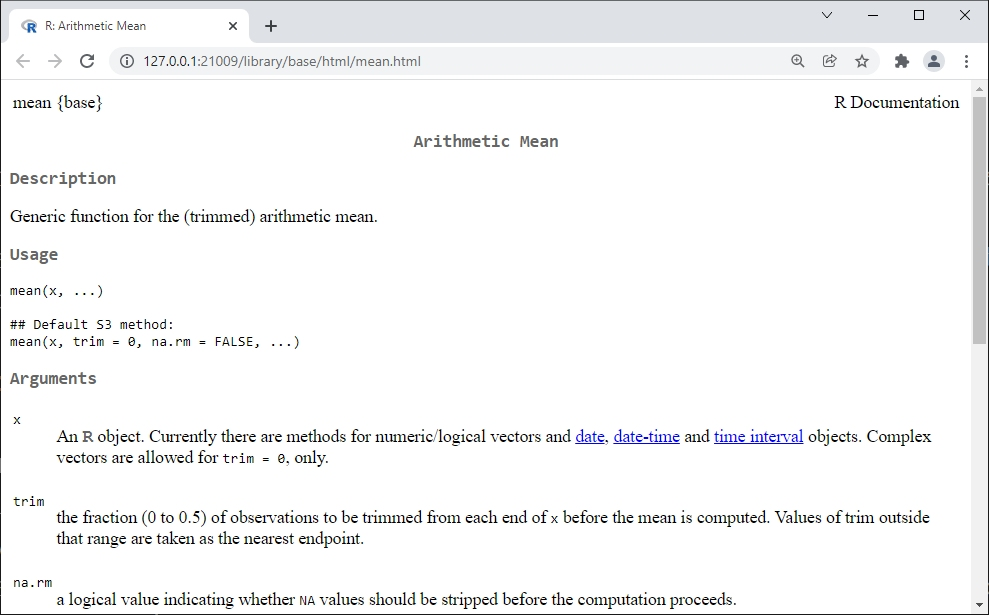
\includegraphics[keepaspectratio]{chapters/../images/02_05.jpg}}

}

\end{figure}%

Some functions belong to a family of related functions that share a
common documentation page. For example, all of the functions related to
the normal distribution share a common page:

\begin{Shaded}
\begin{Highlighting}[]
\NormalTok{?dnorm}
\NormalTok{?pnorm}
\NormalTok{?qnorm}
\NormalTok{?rnorm}
\end{Highlighting}
\end{Shaded}

\begin{figure}[H]

\caption{Example R documentation page for a family of related
functions.}

{\centering \pandocbounded{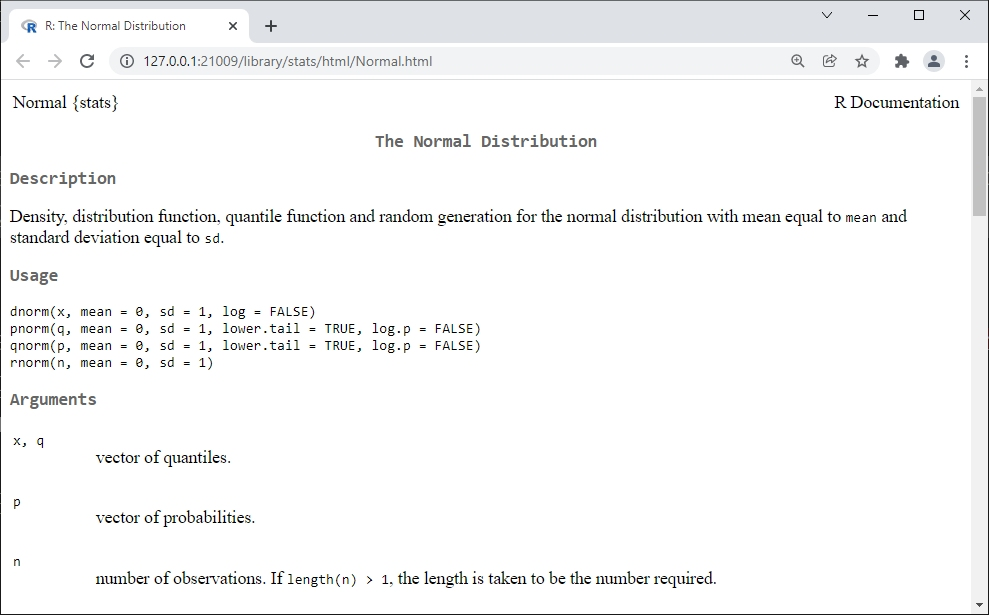
\includegraphics[keepaspectratio]{chapters/../images/02_06.jpg}}

}

\end{figure}%

You can also search for help on functions in packages that are not
attached. Or, you might want to know about a function but don't know
what package it belongs to. Either way, \texttt{??functionname} is a
more general search option that will search any package in your library.
Compare what happens if search for function \texttt{fitdistr()} using
\texttt{?} and \texttt{??} (this function is in package \texttt{MASS},
and so not loaded by default). With \texttt{??}, R searches all
installed packages and returns a browser window with every result that
might match your search term.

\begin{Shaded}
\begin{Highlighting}[]
\NormalTok{?fitdistr}
\NormalTok{??fitdistr}
\end{Highlighting}
\end{Shaded}

\begin{figure}[H]

\caption{Example result of using \texttt{??} to search for an R function
across many packages.}

{\centering \pandocbounded{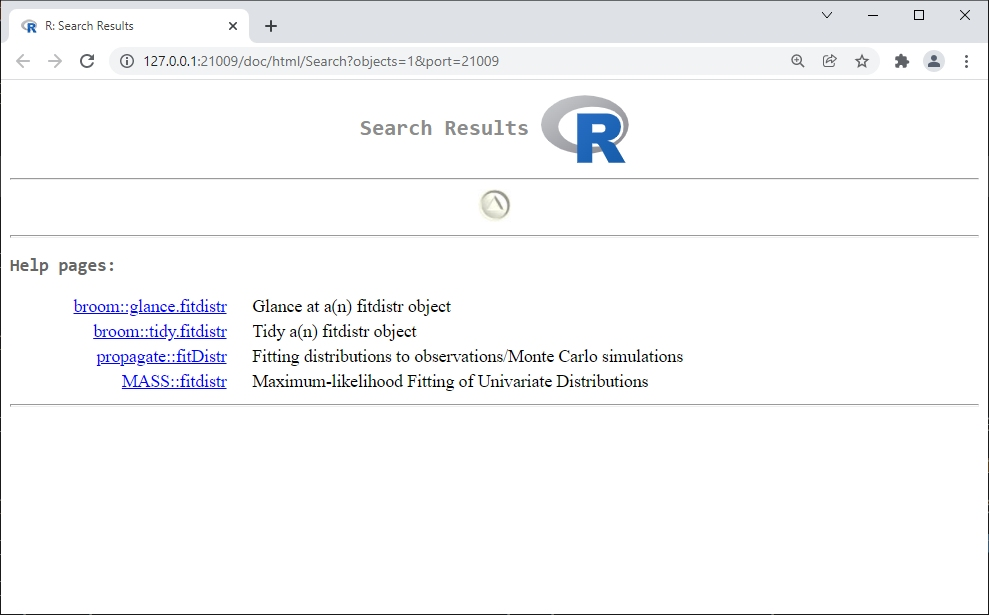
\includegraphics[keepaspectratio]{chapters/../images/02_07.jpg}}

}

\end{figure}%

The R documentation pages all tend to follow the same format:

\textbf{Description}: brief description of what the function does.

\textbf{Usage}: presentation of the function with its arguments in their
typical format and expected order.

\textbf{Arguments}: list of the arguments to the function in order,
their required type/format, and allowed values. This section is very
important. When my code isn't working, the answer to why is usually in
the arguments section.

\textbf{Details}: additional information necessary to use the function.

\textbf{Value}: description of the function's outputs.

\textbf{Source}: description of where the original algorithm or method
came from.

\textbf{References}: citations for the methods used.

\textbf{See also}: list of similar or related R functions.

\textbf{Examples}: illustration of how to use the function. This section
is \textbf{\emph{very}} important. If your code is not working, compare
how you are using the function to the examples. Are you inputs in the
right format? Did you name your arguments or put unnamed arguments in
the wrong order? Careful examination and running of the examples will
usually reveal why your code is not working.

R documentation pages tend to be very terse and include very little in
the way of background or explanation. They are generally meant to
refresh the memory of people already familiar with R and with
statistics, not to educate new R users or inexperienced statisticians.
If you fall into one of the latter categories, or if you are trying to
learn a new function, read on.

\subsubsection{R vignettes}\label{sec-r-faq-help-vig}

A \textbf{vignette} is a document demonstrating the use of an R package
or its functions, with more details and explanation than in the help
files. Not all packages offer vignettes. You can see what vignettes are
available with the command \texttt{vignette()}. Specific vignettes are
accessed by name and package. The examples below show how to get a list
of available vignettes, available vignettes by package, and open
specific vignettes.

\begin{Shaded}
\begin{Highlighting}[]
\CommentTok{\# list vignettes in all installed packages}
\FunctionTok{vignette}\NormalTok{()}
\end{Highlighting}
\end{Shaded}

\begin{figure}[H]

\caption{List of vignettes returned by function \texttt{vignette()}.}

{\centering \pandocbounded{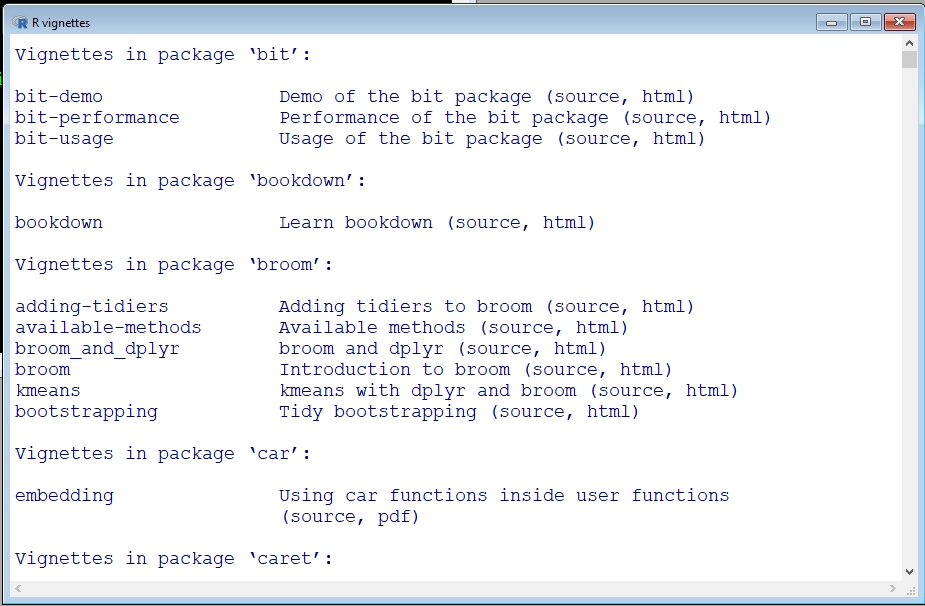
\includegraphics[keepaspectratio]{chapters/../images/02_08.jpg}}

}

\end{figure}%

\begin{Shaded}
\begin{Highlighting}[]
\FunctionTok{vignette}\NormalTok{(}\AttributeTok{package=}\StringTok{"vegan"}\NormalTok{)}
\end{Highlighting}
\end{Shaded}

\begin{figure}[H]

\caption{List of vignettes in a single package, \texttt{vegan}.}

{\centering \pandocbounded{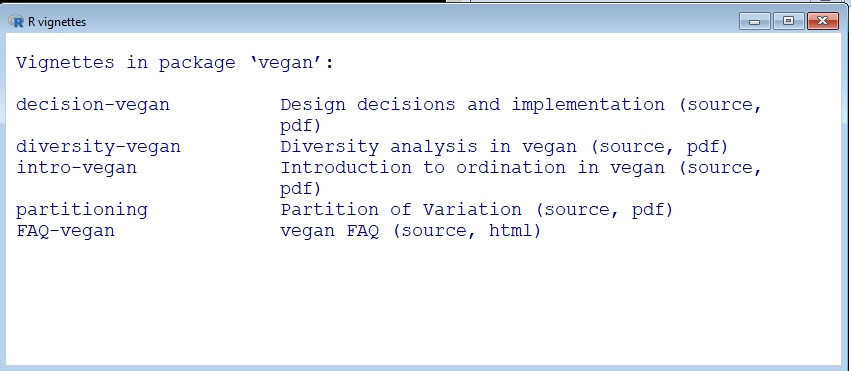
\includegraphics[keepaspectratio]{chapters/../images/02_09.jpg}}

}

\end{figure}%

\begin{Shaded}
\begin{Highlighting}[]
\CommentTok{\# open vignette "intro{-}vegan" in local PDF reader}
\FunctionTok{vignette}\NormalTok{(}\StringTok{"intro{-}vegan"}\NormalTok{, }\AttributeTok{package=}\StringTok{"vegan"}\NormalTok{)}
\end{Highlighting}
\end{Shaded}

\begin{figure}[H]

\caption{A vignette from package \texttt{vegan} in PDF format.}

{\centering \pandocbounded{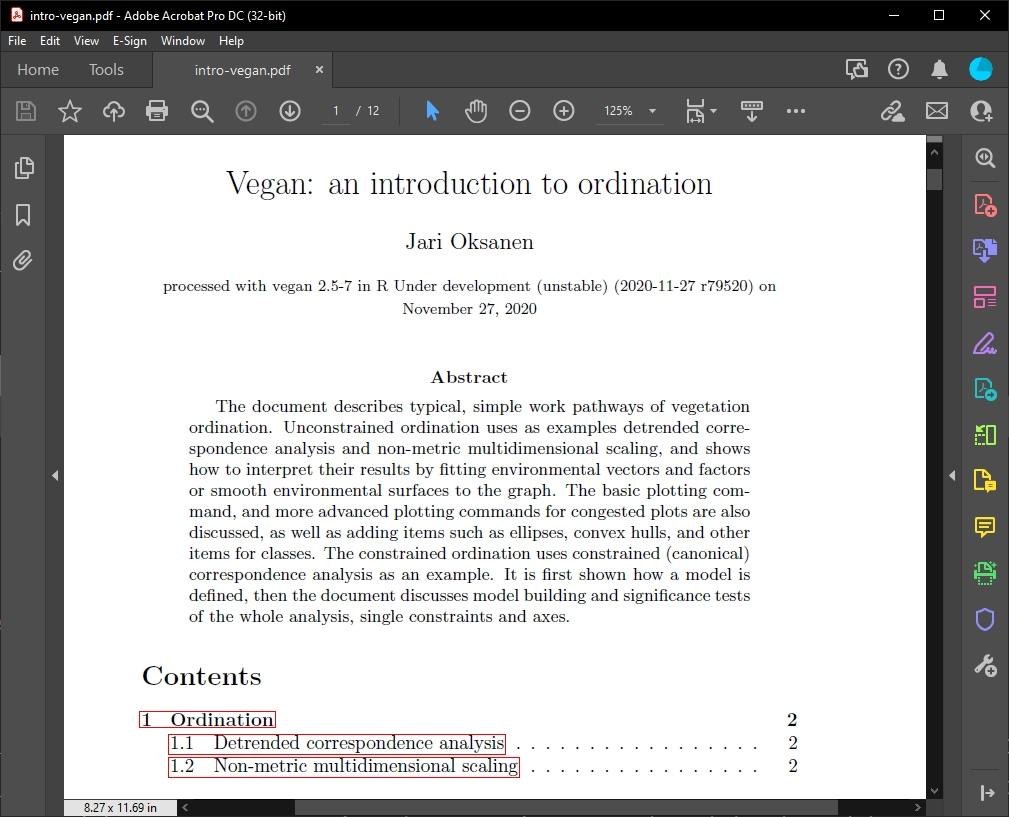
\includegraphics[keepaspectratio]{chapters/../images/02_10.jpg}}

}

\end{figure}%

\subsubsection{Official resources}\label{sec-r-faq-help-off}

The R project maintains an
\href{https://www.r-project.org/help.html}{official help page} with
lists of places to get help. They also maintain a
\href{https://cran.r-project.org/manuals.html}{list of manuals and
documentation}. If you want a handy desk reference, you could do worse
than the
\href{https://cran.r-project.org/doc/contrib/Short-refcard.pdf}{R
reference card} (accessed 2021-12-21).

The \href{https://www.jstatsoft.org/index}{Journal of Statistical
Software} publishes papers about new statistical algorithms and software
packages. Many of its papers are about new R packages and applications.
The papers about new R packages and methods often include extensive code
examples.

\subsubsection{R task views}\label{r-task-views}

The \href{https://cran.r-project.org/web/views/}{Task Views} on CRAN
contain frequently updated lists of packages that are useful for
specific domains. For example, ecologists might check the
\href{https://cran.r-project.org/web/views/Environmetrics.html}{Environmetrics},
\href{https://cran.r-project.org/web/views/Hydrology.html}{Hydrology} or
\href{https://cran.r-project.org/web/views/Spatial.html}{Spatial} task
views. Paleontologists might be more interested in
\href{https://cran.r-project.org/web/views/Paleontology.html}{Paleontology}
or
\href{https://cran.r-project.org/web/views/Phylogenetics.html}{Phylogenetics}.
Physiologists and biochemists might be interested in
\href{https://cran.r-project.org/web/views/Pharmacokinetics.html}{Pharmacokinetics},
\href{https://cran.r-project.org/web/views/ClinicalTrials.html}{Clinical
Trials}, or
\href{https://cran.r-project.org/web/views/Survival.html}{Survival}.
I've spent a lot of time in the
\href{https://cran.r-project.org/web/views/Bayesian.html}{Bayesian},
\href{https://cran.r-project.org/web/views/NumericalMathematics.html}{Numerical
Mathematics}, and
\href{https://cran.r-project.org/web/views/MachineLearning.html}{Machine
Learning} task views. There's something for everyone\ldots even a
\href{https://cran.r-project.org/web/views/TeachingStatistics.html}{Teaching
Statistics} task view with resources to help you learn R and stats at
the same time.

(All links accessed 2025-08-06).

\subsubsection{R mailing lists}\label{sec-r-faq-help-mail}

If your question has been asked before---and this is very likely---there
may be an answer waiting for you on the
\href{https://www.r-project.org/mail.html}{R Help mailing list}. Results
from the R help mailing list will usually show up in Google results. You
can submit a question to the R mailing list, but be very cautious about
doing so. You will need to provide a short, clear, reproducible example
in your question so that other people can see the issue you are
having\footnote{This means a \emph{very} minimal code example that
  people can use to get the same problem that you are having. Don't post
  your entire dataset or include many lines of pre-processing steps or
  other code that led up to your problem. Use base R functions or
  built-in datasets to create a small dataset or set of values that will
  immediately provoke the same error code. Often the process of doing
  this will help you solve your own problem!}. You also need to be sure
that your question hasn't been asked before. Some members of the mailing
list will respond with great hostility and condescension if you fail to
follow those rules.

There are several \href{https://stat.ethz.ch/mailman/listinfo}{special
interest groups (SIG)}, e-mail mailing lists for R users who work in
specific fields. For example,
\href{https://stat.ethz.ch/mailman/listinfo/r-sig-ecology}{R-sig-ecology}
is an e-mail list for ecologists who use R. Other SIG of interest to
biologists include
\href{https://stat.ethz.ch/mailman/listinfo/r-sig-genetics}{R-sig-genetics}
for genetics,
\href{https://stat.ethz.ch/mailman/listinfo/r-sig-mixed-models}{R-sig-mixed-models}
for mixed models,
\href{https://stat.ethz.ch/mailman/listinfo/r-sig-phylo}{R-sig-phylo}
for phylogenetics and related methods, and
\href{https://stat.ethz.ch/mailman/listinfo/r-sig-geo}{R-sig-Geo} for
GIS and spatial analysis.

\subsubsection{Unofficial online resources}\label{sec-r-faq-help-unoff}

Unofficial resources are becoming more and more abundant and useful. One
of the most important sources for R help is
\href{https://stackoverflow.com}{StackOverflow}. StackOverflow is a
hugely popular forum site where programmers ask and answer questions,
and has an active \href{https://stackoverflow.com/questions/tagged/r}{R
section}. When (not if) you find a solution on StackOverflow, include a
link to the answer in your code as a comment. This can save you some
headache down the line when you need to remember how you solved a
problem. Other useful resources include
\href{https://rseek.org/}{RSeek.org}, a search engine for R resources;
and \href{https://www.r-bloggers.com/}{R-Bloggers}, which aggregates
many blogs about R and statistics.

Many R users maintain blogs or websites that may or may not be
aggregated on R-Bloggers. You can usually find these via a Google
search. I have used the pages on
\href{https://www.statmethods.net/}{Quick-R} many times. The UCLA
Statistical Consulting Group has an
\href{https://stats.oarc.ucla.edu/r/}{excellent collection of
tutorials}.

\subsubsection{R books}\label{sec-r-faq-help-books}

The last few years have seen an explosion of books published
specifically about the R language and its uses. Some of these books are
general introductions to R and statistics; others are very domain
specific. Inclusion of a book here does not constitute specific
endorsement. I own some of these, but others are included because they
are common R-related references that you might find helpful.

\begin{itemize}
\tightlist
\item
  The \href{https://www.springer.com/series/6991}{Use R! series}
  contains many high-quality general and domain-specific books, although
  some of the older titles are a bit dated. For example:

  \begin{itemize}
  \tightlist
  \item
    A Beginner's Guide to R by Alain Zuur et al.
  \item
    Data Manipulation with R by Phil Spector
  \item
    Introductory time series with R by P.S.P. Cowperthwaite and A.V.
    Metcalfe.
  \item
    Bayesian computation with R by Jim Albert
  \item
    Introductory Statistics with R by Peter Dalgaard
  \item
    Morphometrics with R by Julien Claude
  \end{itemize}
\item
  The R Book by Michael Crawley
\item
  Advanced R by Hadley Wickham
\item
  R for Dummies by Andrie DeVries
\end{itemize}

When I was first starting out with R I found several books invaluable.
Having code examples printed where I could highlight, annotate, etc.,
was really helpful. Over time I've found myself relying less on
textbooks and more on online sources (especially StackOverflow). Still,
a there are a few books that I use frequently, for their statistical
exposition more than their code examples. At least one of Bolker (2008),
Kéry (2010), Legendre and Legendre (2012), Zuur \emph{et al.} (2007),
and {Zuur \emph{et al.}} (2009a) is usually on my desk at any given
time.

\subsubsection{Two reminders}\label{sec-r-faq-help-two}

I said it at the beginning of this section, and it bears repeating:
\textbf{\emph{Don't panic!}} R has a steep learning curve, but the
pay-off is worth it. There are plenty of resources and people out there
who can help you.

Finally, be sure to \textbf{\emph{read the manual}} when you are stuck.
The R help pages and code examples usually have a solution. Make sure
your inputs are in the right format. Check for syntax and spelling
error--including capitalization! As a funny meme on I saw on Reddit
said, \emph{6 hours of debugging can save you 5 minutes of reading
documentation}.

\chapter{R data types and objects}\label{sec-object}

\section{R data types}\label{sec-object-type}

In R, data are stored in \textbf{objects} with a well-defined structure.
The structures of these objects can facilitate manipulating and
retrieving your data. The structure of an R object is determined by its
\textbf{class}. The format of data (i.e., the kinds of values contained
in an object) is referred to as the data \textbf{type}. Most R users
only encounter types when trying to understand error messages. This is
because many R functions will return errors if their inputs are not of
the correct type.

\subsection{Character type}\label{character-type}

\textbf{Character} data are text strings. They are input and printed
using quotation marks (\texttt{""}). Note that straight quotes are used.
No other kind of quotation mark is valid in R code. If you paste in text
from another program that has ``curly quotes'' (e.g., from Word), you
will get an error.

\begin{Shaded}
\begin{Highlighting}[]
\NormalTok{a }\OtherTok{\textless{}{-}} \FunctionTok{c}\NormalTok{(}\StringTok{"aardvark"}\NormalTok{, }\StringTok{"bunny"}\NormalTok{, }\StringTok{"caterpillar"}\NormalTok{)}
\NormalTok{a}
\end{Highlighting}
\end{Shaded}

\begin{verbatim}
[1] "aardvark"    "bunny"       "caterpillar"
\end{verbatim}

Notice that in the command above the values in \texttt{a} are defined in
quotation marks. Without quotation marks, R would interpret those words
as the names of objects. For example:

\begin{Shaded}
\begin{Highlighting}[]
\NormalTok{caterpillar }\OtherTok{\textless{}{-}} \StringTok{"lion"}
\FunctionTok{c}\NormalTok{(}\StringTok{"aardvark"}\NormalTok{, }\StringTok{"bunny"}\NormalTok{, caterpillar)}
\end{Highlighting}
\end{Shaded}

\begin{verbatim}
[1] "aardvark" "bunny"    "lion"    
\end{verbatim}

There are some special character vectors pre-built into R that can be
useful in programming: \texttt{letters} returns the lower case letters
a-z, while \texttt{LETTERS} returns the upper-case letters A-Z.

\begin{Shaded}
\begin{Highlighting}[]
\NormalTok{letters}
\DocumentationTok{\#\#  [1] "a" "b" "c" "d" "e" "f" "g" "h" "i" "j" "k" "l" "m" "n" "o" "p" "q" "r" "s"}
\DocumentationTok{\#\# [20] "t" "u" "v" "w" "x" "y" "z"}
\NormalTok{LETTERS}
\DocumentationTok{\#\#  [1] "A" "B" "C" "D" "E" "F" "G" "H" "I" "J" "K" "L" "M" "N" "O" "P" "Q" "R" "S"}
\DocumentationTok{\#\# [20] "T" "U" "V" "W" "X" "Y" "Z"}
\NormalTok{letters[}\DecValTok{11}\SpecialCharTok{:}\DecValTok{20}\NormalTok{]}
\DocumentationTok{\#\#  [1] "k" "l" "m" "n" "o" "p" "q" "r" "s" "t"}
\end{Highlighting}
\end{Shaded}

Similarly, \texttt{month.name} and \texttt{month.abb} contain the names
of the 12 months and their 3 letter abbreviations, respectively. The
latter is very useful for making figure axes.

\begin{Shaded}
\begin{Highlighting}[]
\FunctionTok{plot}\NormalTok{(}\DecValTok{1}\SpecialCharTok{:}\DecValTok{12}\NormalTok{, }\FunctionTok{runif}\NormalTok{(}\DecValTok{12}\NormalTok{), }\AttributeTok{xaxt=}\StringTok{"n"}\NormalTok{, }\AttributeTok{xlab=} \StringTok{"Month"}\NormalTok{)}
\FunctionTok{axis}\NormalTok{(}\AttributeTok{side=}\DecValTok{1}\NormalTok{, }\AttributeTok{at=}\DecValTok{1}\SpecialCharTok{:}\DecValTok{12}\NormalTok{, }\AttributeTok{labels=}\NormalTok{month.abb)}
\end{Highlighting}
\end{Shaded}

\pandocbounded{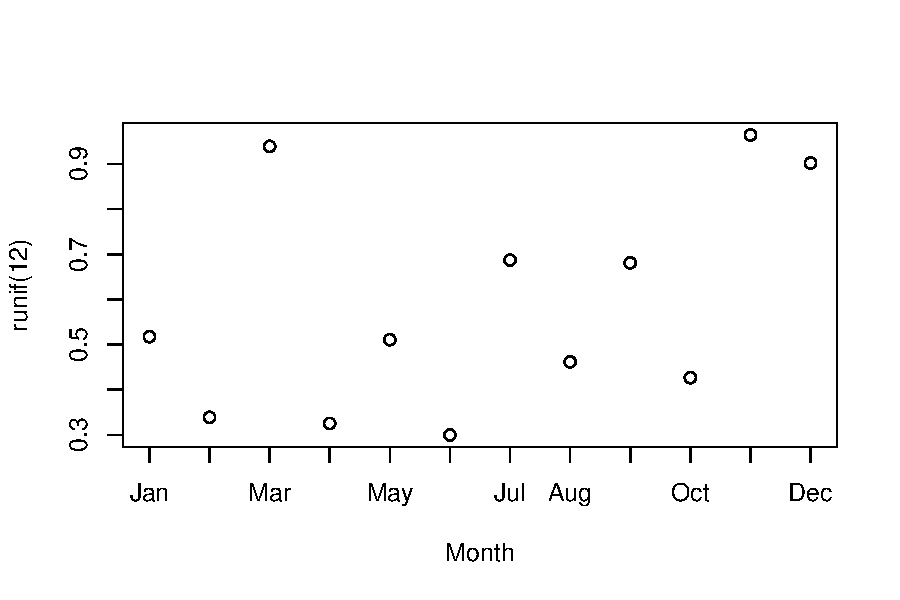
\includegraphics[keepaspectratio]{chapters/ch03_files/figure-pdf/unnamed-chunk-4-1.pdf}}

As an aside, the function \texttt{substr()} extracts parts of character
strings (``substring''). One application is getting one letter
abbreviations of the months for a figure axis. The example below selects
from the month names starting and ending at character 1. The argument
\texttt{xaxt="n"} in \texttt{plot()} suppresses the \emph{x}-axis, so we
can add our own with \texttt{axis()}.

\begin{Shaded}
\begin{Highlighting}[]
\NormalTok{use.months }\OtherTok{\textless{}{-}} \FunctionTok{substr}\NormalTok{(month.name, }\DecValTok{1}\NormalTok{, }\DecValTok{1}\NormalTok{)}
\FunctionTok{plot}\NormalTok{(}\DecValTok{1}\SpecialCharTok{:}\DecValTok{12}\NormalTok{, }\FunctionTok{runif}\NormalTok{(}\DecValTok{12}\NormalTok{), }\AttributeTok{xaxt=}\StringTok{"n"}\NormalTok{, }\AttributeTok{xlab=} \StringTok{"Month"}\NormalTok{)}
\FunctionTok{axis}\NormalTok{(}\AttributeTok{side=}\DecValTok{1}\NormalTok{, }\AttributeTok{at=}\DecValTok{1}\SpecialCharTok{:}\DecValTok{12}\NormalTok{, }\AttributeTok{labels=}\NormalTok{use.months)}
\end{Highlighting}
\end{Shaded}

\pandocbounded{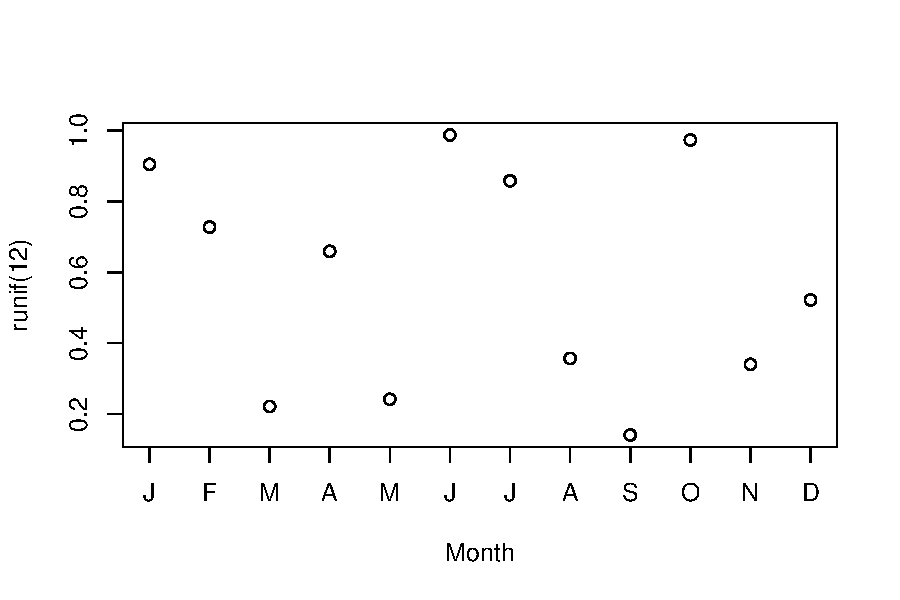
\includegraphics[keepaspectratio]{chapters/ch03_files/figure-pdf/unnamed-chunk-5-1.pdf}}

\subsection{Numeric type}\label{numeric-type}

Most data are stored as the \textbf{numeric} type. This includes
\textbf{floating point numbers} (e.g., \texttt{3.14159} or
\texttt{3.14e0}). Floating point numbers are referred to as type
``double'' in R (short for
``\href{*https://en.wikipedia.org/wiki/Double-precision_floating-point_format}{double-precision
floating point}'').

\begin{Shaded}
\begin{Highlighting}[]
\FunctionTok{typeof}\NormalTok{(}\DecValTok{2}\NormalTok{)}
\end{Highlighting}
\end{Shaded}

\begin{verbatim}
[1] "double"
\end{verbatim}

\begin{Shaded}
\begin{Highlighting}[]
\FunctionTok{typeof}\NormalTok{(pi)}
\end{Highlighting}
\end{Shaded}

\begin{verbatim}
[1] "double"
\end{verbatim}

\subsection{Integer type}\label{integer-type}

\textbf{Integers} are numbers with no fractional components. Some
numbers are stored as integers, but integers are not always
interchangeable with floating point numbers. For example, some
probability distribution functions return integer values rather than
floating point values (e.g., binomial or Poisson). This can be
problematic if very large numbers are expected because the maximum
integer value in R is much smaller than the maximum floating-point
value. Note that having the type \texttt{integer} in R and \emph{being
an integer} from a mathematical standpoint are not synonymous.

\begin{Shaded}
\begin{Highlighting}[]
\CommentTok{\# numbers are double by default:}
\FunctionTok{typeof}\NormalTok{(}\DecValTok{7}\NormalTok{)}
\DocumentationTok{\#\# [1] "double"}

\CommentTok{\# convert to integer with as.integer():}
\FunctionTok{typeof}\NormalTok{(}\FunctionTok{as.integer}\NormalTok{(}\DecValTok{7}\NormalTok{))}
\DocumentationTok{\#\# [1] "integer"}

\CommentTok{\# test whether input is integer type:}
\FunctionTok{is.integer}\NormalTok{(}\DecValTok{7}\NormalTok{)}
\DocumentationTok{\#\# [1] FALSE}

\CommentTok{\# test whether input is numeric type:}
\FunctionTok{is.numeric}\NormalTok{(}\DecValTok{7}\NormalTok{)}
\DocumentationTok{\#\# [1] TRUE}

\CommentTok{\# some functions return integer type as output:}
\FunctionTok{typeof}\NormalTok{(}\FunctionTok{rbinom}\NormalTok{(}\DecValTok{1}\NormalTok{, }\DecValTok{10}\NormalTok{, }\FloatTok{0.7}\NormalTok{))}
\DocumentationTok{\#\# [1] "integer"}

\CommentTok{\# 7 is mathematically an integer (7 mod 1 == 0),}
\CommentTok{\# but is not of integer type in R}
\DecValTok{7} \SpecialCharTok{\%\%} \DecValTok{1}
\DocumentationTok{\#\# [1] 0}
\end{Highlighting}
\end{Shaded}

Integers are used as indices for subsetting and accessing other objects.
A sequence of integers can be made using the colon operator as follows:

\begin{Shaded}
\begin{Highlighting}[]
\NormalTok{a }\OtherTok{\textless{}{-}} \DecValTok{1}\SpecialCharTok{:}\DecValTok{10}
\NormalTok{a}
\DocumentationTok{\#\#  [1]  1  2  3  4  5  6  7  8  9 10}
\FunctionTok{typeof}\NormalTok{(a)}
\DocumentationTok{\#\# [1] "integer"}
\end{Highlighting}
\end{Shaded}

An important consequence of using integers as index values is that
object dimensions are limited to the \textbf{R integer limit}. This is
probably not a major concern for most users. Your machine will likely
run out of memory before you could make such an object anyway. You can
check the integer limit on your machine with this line:

\begin{Shaded}
\begin{Highlighting}[]
\NormalTok{.Machine}\SpecialCharTok{$}\NormalTok{integer.max}
\end{Highlighting}
\end{Shaded}

\begin{verbatim}
[1] 2147483647
\end{verbatim}

On my machine, this is about 2.14 × 10\textsuperscript{9}. If you need
data objects with dimensions larger than this, you may need to either
use a specialized R package that can handle huge objects, or you may
need rethink what you are doing.

\subsection{Logical type}\label{logical-type}

The \textbf{logical} data type stores \texttt{TRUE} and \texttt{FALSE}
values. Note that \texttt{TRUE} and \texttt{FALSE} are always written in
capital letters, without quotation marks. Logical values are produced by
logical tests, such as the test for equality using \texttt{==}:

\begin{Shaded}
\begin{Highlighting}[]
\DecValTok{1}\SpecialCharTok{+}\DecValTok{1} \SpecialCharTok{==} \DecValTok{2}            
\DocumentationTok{\#\# [1] TRUE}
\FunctionTok{typeof}\NormalTok{(}\DecValTok{1}\SpecialCharTok{+}\DecValTok{1} \SpecialCharTok{==} \DecValTok{2}\NormalTok{)    }
\DocumentationTok{\#\# [1] "logical"}
\FunctionTok{typeof}\NormalTok{(}\DecValTok{1}\SpecialCharTok{+}\DecValTok{1} \SpecialCharTok{==} \DecValTok{3}\NormalTok{)    }
\DocumentationTok{\#\# [1] "logical"}
\end{Highlighting}
\end{Shaded}

Another useful test you can do is to test whether elements of one set
are in another:

\begin{Shaded}
\begin{Highlighting}[]
\DecValTok{5} \SpecialCharTok{\%in\%} \DecValTok{1}\SpecialCharTok{:}\DecValTok{10}
\DocumentationTok{\#\# [1] TRUE}
\DecValTok{5} \SpecialCharTok{\%in\%} \DecValTok{6}\SpecialCharTok{:}\DecValTok{10}
\DocumentationTok{\#\# [1] FALSE}
\DecValTok{1}\SpecialCharTok{:}\DecValTok{10} \SpecialCharTok{\%in\%} \DecValTok{5}\SpecialCharTok{:}\DecValTok{15}
\DocumentationTok{\#\#  [1] FALSE FALSE FALSE FALSE  TRUE  TRUE  TRUE  TRUE  TRUE  TRUE}
\end{Highlighting}
\end{Shaded}

You can test with inequalities:

\begin{Shaded}
\begin{Highlighting}[]
\DecValTok{2} \SpecialCharTok{\textgreater{}=} \DecValTok{1}
\DocumentationTok{\#\# [1] TRUE}
\DecValTok{3} \SpecialCharTok{\textless{}} \DecValTok{2}
\DocumentationTok{\#\# [1] FALSE}
\end{Highlighting}
\end{Shaded}

Sometimes it can be useful to store logical values as 1 or 0. You can do
this by multiplying a logical by 1 or using function
\texttt{as.numeric}.

\begin{Shaded}
\begin{Highlighting}[]
\DecValTok{1}\SpecialCharTok{*}\NormalTok{(}\DecValTok{1}\SpecialCharTok{+}\DecValTok{1} \SpecialCharTok{==} \DecValTok{2}\NormalTok{)}
\DocumentationTok{\#\# [1] 1}
\DecValTok{1}\SpecialCharTok{*}\NormalTok{(}\DecValTok{1}\SpecialCharTok{+}\DecValTok{1} \SpecialCharTok{==} \DecValTok{3}\NormalTok{)}
\DocumentationTok{\#\# [1] 0}
\FunctionTok{typeof}\NormalTok{(}\DecValTok{1}\SpecialCharTok{+}\DecValTok{1} \SpecialCharTok{==} \DecValTok{2}\NormalTok{)}
\DocumentationTok{\#\# [1] "logical"}
\FunctionTok{typeof}\NormalTok{(}\DecValTok{1}\SpecialCharTok{*}\NormalTok{(}\DecValTok{1}\SpecialCharTok{+}\DecValTok{1} \SpecialCharTok{==} \DecValTok{2}\NormalTok{))}
\DocumentationTok{\#\# [1] "double"}
\FunctionTok{typeof}\NormalTok{(}\FunctionTok{as.numeric}\NormalTok{(}\DecValTok{1}\SpecialCharTok{+}\DecValTok{1} \SpecialCharTok{==} \DecValTok{1}\SpecialCharTok{:}\DecValTok{5}\NormalTok{))}
\DocumentationTok{\#\# [1] "double"}
\end{Highlighting}
\end{Shaded}

The \texttt{!} symbol \textbf{negates} or \textbf{reverses} logical
values. It does not negate logical values stored as numbers.

\begin{Shaded}
\begin{Highlighting}[]
\DecValTok{2}\SpecialCharTok{+}\DecValTok{2} \SpecialCharTok{==} \DecValTok{4}
\DocumentationTok{\#\# [1] TRUE}
\SpecialCharTok{!} \DecValTok{2}\SpecialCharTok{+}\DecValTok{2} \SpecialCharTok{==} \DecValTok{4}
\DocumentationTok{\#\# [1] FALSE}
\DecValTok{1}\SpecialCharTok{:}\DecValTok{10} \SpecialCharTok{\%in\%} \DecValTok{5}\SpecialCharTok{:}\DecValTok{15}
\DocumentationTok{\#\#  [1] FALSE FALSE FALSE FALSE  TRUE  TRUE  TRUE  TRUE  TRUE  TRUE}
\SpecialCharTok{!}\DecValTok{1}\SpecialCharTok{:}\DecValTok{10} \SpecialCharTok{\%in\%} \DecValTok{5}\SpecialCharTok{:}\DecValTok{15}
\DocumentationTok{\#\#  [1]  TRUE  TRUE  TRUE  TRUE FALSE FALSE FALSE FALSE FALSE FALSE}
\end{Highlighting}
\end{Shaded}

The \texttt{any()} and \texttt{all()} functions test to see if any
values in a set of logical values is true (\texttt{any()}) or if all of
them are true (\texttt{all()}).

\begin{Shaded}
\begin{Highlighting}[]
\DecValTok{1}\SpecialCharTok{:}\DecValTok{5} \SpecialCharTok{\textless{}} \DecValTok{3}
\DocumentationTok{\#\# [1]  TRUE  TRUE FALSE FALSE FALSE}
\FunctionTok{any}\NormalTok{(}\DecValTok{1}\SpecialCharTok{:}\DecValTok{5} \SpecialCharTok{\textless{}} \DecValTok{3}\NormalTok{)}
\DocumentationTok{\#\# [1] TRUE}
\FunctionTok{all}\NormalTok{(}\DecValTok{1}\SpecialCharTok{:}\DecValTok{5} \SpecialCharTok{\textless{}} \DecValTok{3}\NormalTok{)}
\DocumentationTok{\#\# [1] FALSE}
\end{Highlighting}
\end{Shaded}

\texttt{TRUE} and \texttt{FALSE} can also be abbreviated as uppercase
\texttt{T} or \texttt{F}, but not lowercase \texttt{t} or \texttt{f}.
This means that you should \textbf{\emph{not}} create objects with names
\texttt{T}, \texttt{F}, \texttt{TRUE}, etc. (don't name an object
\texttt{t} either, because that is the name of the transpose function).
The code block below illustrates the mischief that can be created by
naming an object \texttt{T} and masking the built-in value for true.

\begin{Shaded}
\begin{Highlighting}[]
\CommentTok{\# (1+1==2) is true.}
\NormalTok{T }\SpecialCharTok{==}\NormalTok{ (}\DecValTok{1}\SpecialCharTok{+}\DecValTok{1}\SpecialCharTok{==}\DecValTok{2}\NormalTok{)}
\DocumentationTok{\#\# [1] TRUE}

\CommentTok{\# make a new object T with value 3}
\NormalTok{T }\OtherTok{\textless{}{-}} \DecValTok{3}

\CommentTok{\# (1+1==2) is now not true, unless it is}
\NormalTok{T }\SpecialCharTok{==}\NormalTok{ (}\DecValTok{1}\SpecialCharTok{+}\DecValTok{1}\SpecialCharTok{==}\DecValTok{2}\NormalTok{)}
\DocumentationTok{\#\# [1] FALSE}
\ConstantTok{TRUE} \SpecialCharTok{==}\NormalTok{ (}\DecValTok{1}\SpecialCharTok{+}\DecValTok{1}\SpecialCharTok{==}\DecValTok{2}\NormalTok{)}
\DocumentationTok{\#\# [1] TRUE}

\CommentTok{\# remove the troublesome T}
\FunctionTok{rm}\NormalTok{(T)}

\CommentTok{\# things are back to normal}
\NormalTok{T }\SpecialCharTok{==}\NormalTok{ (}\DecValTok{1}\SpecialCharTok{+}\DecValTok{1}\SpecialCharTok{==}\DecValTok{2}\NormalTok{)}
\DocumentationTok{\#\# [1] TRUE}
\end{Highlighting}
\end{Shaded}

\subsection{Special values}\label{sec-object-type-spec}

\subsubsection{\texorpdfstring{Missing values
\texttt{NA}}{Missing values NA}}\label{sec-object-type-spec-na}

Missing data in R are labeled as \texttt{NA}, or ``Not Available''. This
is R-speak for a blank or missing value. Some functions can ignore
\texttt{NA}, some cannot. Some functions produce \texttt{NA} when you
supply them with improper inputs. Note that this is a feature, not a
bug. R is set up to produce \texttt{NA} by default in many cases to help
you track down where the missing values are coming from. Function
\texttt{is.na()} tests to see if a value is missing.

\begin{Shaded}
\begin{Highlighting}[]
\NormalTok{aa }\OtherTok{\textless{}{-}} \FunctionTok{c}\NormalTok{(}\DecValTok{1}\SpecialCharTok{:}\DecValTok{8}\NormalTok{,}\ConstantTok{NA}\NormalTok{)}

\NormalTok{aa }\SpecialCharTok{+} \DecValTok{2}
\DocumentationTok{\#\# [1]  3  4  5  6  7  8  9 10 NA}

\CommentTok{\# returns NA}
\FunctionTok{mean}\NormalTok{(aa)}
\DocumentationTok{\#\# [1] NA}

\CommentTok{\# option to ignore NA values}
\FunctionTok{mean}\NormalTok{(aa,}\AttributeTok{na.rm=}\ConstantTok{TRUE}\NormalTok{)      }
\DocumentationTok{\#\# [1] 4.5}

\CommentTok{\# test for NA}
\FunctionTok{is.na}\NormalTok{(aa)               }
\DocumentationTok{\#\# [1] FALSE FALSE FALSE FALSE FALSE FALSE FALSE FALSE  TRUE}

\CommentTok{\# which elements are NA?}
\FunctionTok{which}\NormalTok{(}\FunctionTok{is.na}\NormalTok{(aa))        }
\DocumentationTok{\#\# [1] 9}

\CommentTok{\# remove NA elements}
\NormalTok{aa[}\SpecialCharTok{{-}}\FunctionTok{which}\NormalTok{(}\FunctionTok{is.na}\NormalTok{(aa))]   }
\DocumentationTok{\#\# [1] 1 2 3 4 5 6 7 8}

\CommentTok{\# another way to remove NA elements}
\NormalTok{aa[}\FunctionTok{which}\NormalTok{(}\SpecialCharTok{!}\FunctionTok{is.na}\NormalTok{(aa))]   }
\DocumentationTok{\#\# [1] 1 2 3 4 5 6 7 8}

\CommentTok{\# returns NA: Poisson distribution supported only on [0,+Inf]}
\FunctionTok{rpois}\NormalTok{(}\DecValTok{10}\NormalTok{,}\SpecialCharTok{{-}}\DecValTok{2}\NormalTok{) }
\DocumentationTok{\#\#  [1] NA NA NA NA NA NA NA NA NA NA}
\end{Highlighting}
\end{Shaded}

\subsubsection{Infinities}\label{sec-object-type-spec-inf}

Positive and negative infinity (\(+\infty\) and \(-\infty\)) are labeled
in R as \texttt{Inf} and \texttt{–Inf}. Dividing a non-zero number by 0
produces \texttt{Inf}. Taking the log of 0 produces \texttt{–Inf}.
Trying to generate a value greater than R's maximal value can produce
\texttt{Inf}.

\begin{Shaded}
\begin{Highlighting}[]
\DecValTok{5}\SpecialCharTok{/}\DecValTok{0}
\DocumentationTok{\#\# [1] Inf}
\FunctionTok{log}\NormalTok{(}\DecValTok{0}\NormalTok{)}
\DocumentationTok{\#\# [1] {-}Inf}
\DecValTok{10}\SpecialCharTok{\^{}}\DecValTok{10}\SpecialCharTok{\^{}}\DecValTok{10}
\DocumentationTok{\#\# [1] Inf}
\end{Highlighting}
\end{Shaded}

\subsubsection{Undefined values}\label{sec-object-type-spec-nan}

Some values that are undefined are labeled \texttt{NaN} (not a number).
This means that a value is undefined, not that it is missing (which
would be \texttt{NA}) or infinite (which would be \texttt{Inf} or
\texttt{-Inf}). Dividing 0 by 0, or taking the log of a negative number,
produces \texttt{NaN}. The function \texttt{is.nan()} tests to see if a
value is \texttt{NaN}.

\begin{Shaded}
\begin{Highlighting}[]
\DecValTok{0}\SpecialCharTok{/}\DecValTok{0}
\DocumentationTok{\#\# [1] NaN}
\FunctionTok{log}\NormalTok{(}\SpecialCharTok{{-}}\DecValTok{1}\NormalTok{)}
\DocumentationTok{\#\# [1] NaN}
\end{Highlighting}
\end{Shaded}

\subsubsection{Special values are
useful}\label{sec-object-type-spec-why}

Why are there so many special values? Often they are meant to help track
down where erroneous values are coming from. If every undefined value
returned the same symbol (or word, etc.), then it would be harder to
know why a program was returning undefined values. Instead, the
different results help point the way:

\begin{itemize}
\tightlist
\item
  \texttt{Inf}: Positive non-zero number divided by 0
\item
  \texttt{-Inf}: Negative non-zero number divided by 0 \emph{or}
  \texttt{log(0)}.
\item
  \texttt{NaN}: \texttt{0/0} or logarithm of a negative number
\end{itemize}

\section{Basic R data structures}\label{sec-object-struct}

In R, data are stored in \textbf{objects} with a well-defined structure.
The structures of these objects can facilitate manipulating and
retrieving your data. The structure of an R object is determined by its
class. The format of data (i.e., the kinds of values contained in an
object) is referred to as the data type.

For a solid introduction to R classes and data types, refer to
\href{https://cran.r-project.org/doc/manuals/r-release/R-intro.html}{An
introduction to R}, one of the official R help manuals. The book
\emph{Data manipulation with R} (Spector 2008) is also good. If you want
to explore the odder and less benign aspects of R data structures, I
recommend the truly excellent
\href{https://www.burns-stat.com/pages/Tutor/R_inferno.pdf}{\emph{The R
Inferno}} (accessed 2025-08-06).

\subsection{Vectors}\label{sec-object-struct-vect}

In R, as in mathematics, a \textbf{vector} is an ordered set of values.
Vectors are a key concept in statistics and linear algebra. For example,
the set \([1,2,3,4,5]\) is a vector. This vector is different than the
set (and vector) \([2,3,1,5,4]\). These sets are different vectors
because even though they contain the same values, those values are in
different orders. In R we could call either of those sets a ``vector''.
Note that we don't call them ``lists'' because a list is a special kind
of object in R that is not synonymous with vector.

As a language designed primarily for statistics, R has a strong emphasis
on vectors and their manipulation. Vectors are probably the simplest
type of data object in R. Understanding them is the key to understanding
other data objects in R.

Another way to think of vectors is as an \textbf{array} with one
dimension, length. In computing, an ``array'' is a systematic
arrangement of similar elements. An array with 1 dimension is a vector.
A two-dimensional array is a \textbf{matrix}, and an array with \(\ge\)
3 dimensions is just called an array. Vectors, matrices, and arrays in R
can be a convenient way to store structured data that are all of the
same type (numeric, logical, character, etc.).

Vectors can be created by the function \texttt{vector()} as well as by
functions specific to the type of value to be stored. The most common
types are \textbf{numeric}, \textbf{logical}, and \textbf{character}.
These hold numbers, logical values, and text, respectively. Each type
has a default value (\texttt{0}, \texttt{FALSE}, and \texttt{""}
(blank), respectively). Notice that in each command below R prints the
results to the console because the resulting vectors are not assigned to
an object.

\begin{Shaded}
\begin{Highlighting}[]
\FunctionTok{vector}\NormalTok{(}\StringTok{"numeric"}\NormalTok{, }\DecValTok{5}\NormalTok{)}
\DocumentationTok{\#\# [1] 0 0 0 0 0}
\FunctionTok{vector}\NormalTok{(}\StringTok{"logical"}\NormalTok{, }\DecValTok{5}\NormalTok{)}
\DocumentationTok{\#\# [1] FALSE FALSE FALSE FALSE FALSE}
\FunctionTok{vector}\NormalTok{(}\StringTok{"character"}\NormalTok{,}\DecValTok{5}\NormalTok{)}
\DocumentationTok{\#\# [1] "" "" "" "" ""}

\CommentTok{\# equivalent to above commands:}
\FunctionTok{numeric}\NormalTok{(}\DecValTok{5}\NormalTok{)}
\DocumentationTok{\#\# [1] 0 0 0 0 0}
\FunctionTok{logical}\NormalTok{(}\DecValTok{5}\NormalTok{)}
\DocumentationTok{\#\# [1] FALSE FALSE FALSE FALSE FALSE}
\FunctionTok{character}\NormalTok{(}\DecValTok{5}\NormalTok{)}
\DocumentationTok{\#\# [1] "" "" "" "" ""}
\end{Highlighting}
\end{Shaded}

Creating vectors this way is cumbersome, but useful when programming
complex tasks. It is usually more efficient, from a memory usage
standpoint, to create an object and fill it later than to create it and
repeatedly change its size.

You can also create vectors by defining their contents. When you do
this, R will guess at the type of vector based on the values you give
it. These guesses are usually okay.

\begin{Shaded}
\begin{Highlighting}[]
\CommentTok{\# numeric:}
\FunctionTok{class}\NormalTok{(}\FunctionTok{runif}\NormalTok{(}\DecValTok{10}\NormalTok{))}
\DocumentationTok{\#\# [1] "numeric"}

\CommentTok{\# integer, which is stored in numeric vectors}
\CommentTok{\# despite being a different type:}
\FunctionTok{class}\NormalTok{(}\DecValTok{1}\SpecialCharTok{:}\DecValTok{5}\NormalTok{)}
\DocumentationTok{\#\# [1] "integer"}
\FunctionTok{is.numeric}\NormalTok{(}\DecValTok{1}\SpecialCharTok{:}\DecValTok{5}\NormalTok{)}
\DocumentationTok{\#\# [1] TRUE}
\end{Highlighting}
\end{Shaded}

Vectors can also be made by putting values together using the function
\texttt{c()} (short for ``combine'' or ``concatenate''). Note that if
you try to combine values of different types, R will convert all values
to character strings.

\begin{Shaded}
\begin{Highlighting}[]
\CommentTok{\# create a vector of numbers}
\NormalTok{my.vec }\OtherTok{\textless{}{-}} \FunctionTok{c}\NormalTok{(}\DecValTok{1}\NormalTok{,}\DecValTok{2}\NormalTok{,}\DecValTok{4}\SpecialCharTok{:}\DecValTok{8}\NormalTok{,}\DecValTok{10}\NormalTok{)}
\NormalTok{my.vec}
\DocumentationTok{\#\# [1]  1  2  4  5  6  7  8 10}

\CommentTok{\# create a vector of character strings}
\NormalTok{my.vec2 }\OtherTok{\textless{}{-}} \FunctionTok{c}\NormalTok{(}\StringTok{"zebra"}\NormalTok{,}\StringTok{"hippo"}\NormalTok{,}\StringTok{"lion"}\NormalTok{,}\StringTok{"rhino"}\NormalTok{,}\StringTok{"rhino"}\NormalTok{)}
\NormalTok{my.vec2}
\DocumentationTok{\#\# [1] "zebra" "hippo" "lion"  "rhino" "rhino"}

\CommentTok{\# create a vector with 1 numeric, 1 character,}
\CommentTok{\# and 1 logical value...all are converted to}
\CommentTok{\# character strings.}
\NormalTok{my.vec3 }\OtherTok{\textless{}{-}} \FunctionTok{c}\NormalTok{(}\DecValTok{1}\NormalTok{,}\StringTok{"hippo"}\NormalTok{,}\DecValTok{1}\SpecialCharTok{+}\DecValTok{1}\SpecialCharTok{==}\DecValTok{3}\NormalTok{)}
\NormalTok{my.vec3}
\DocumentationTok{\#\# [1] "1"     "hippo" "FALSE"}
\end{Highlighting}
\end{Shaded}

Each value within a vector is called an \textbf{element}. Elements of a
vector are accessed by the bracket notation.

\begin{Shaded}
\begin{Highlighting}[]
\CommentTok{\# get some random numbers}
\NormalTok{a }\OtherTok{\textless{}{-}} \FunctionTok{runif}\NormalTok{(}\DecValTok{5}\NormalTok{)}

\CommentTok{\# print to console}
\NormalTok{a          }
\DocumentationTok{\#\# [1] 0.2508072 0.3258648 0.4004049 0.4817464 0.1671091}

\CommentTok{\# 3rd element}
\NormalTok{a[}\DecValTok{3}\NormalTok{]       }
\DocumentationTok{\#\# [1] 0.4004049}

\CommentTok{\# elements 2{-}4}
\NormalTok{a[}\DecValTok{2}\SpecialCharTok{:}\DecValTok{4}\NormalTok{]     }
\DocumentationTok{\#\# [1] 0.3258648 0.4004049 0.4817464}

\CommentTok{\# elements other than 1}
\NormalTok{a[}\SpecialCharTok{{-}}\DecValTok{1}\NormalTok{]      }
\DocumentationTok{\#\# [1] 0.3258648 0.4004049 0.4817464 0.1671091}

\CommentTok{\# elements other than 1 and 2}
\NormalTok{a[}\SpecialCharTok{{-}}\FunctionTok{c}\NormalTok{(}\DecValTok{1}\SpecialCharTok{:}\DecValTok{2}\NormalTok{)] }
\DocumentationTok{\#\# [1] 0.4004049 0.4817464 0.1671091}
\end{Highlighting}
\end{Shaded}

You can inspect a vector (or any object) by printing it to the console.
Do this by typing the object's name into the console at the command
prompt \texttt{\textgreater{}} and pressing ENTER.

\begin{Shaded}
\begin{Highlighting}[]
\NormalTok{my.vec}
\end{Highlighting}
\end{Shaded}

\begin{verbatim}
[1]  1  2  4  5  6  7  8 10
\end{verbatim}

The \texttt{{[}1{]}} at the start of the line with your results
indicates that that line starts with the first element of the object. If
an object runs over to multiple lines, each line will begin with the
index of the first value printed on that line. Make your console window
narrower and try this command:

\begin{Shaded}
\begin{Highlighting}[]
\FunctionTok{runif}\NormalTok{(}\DecValTok{20}\NormalTok{)}
\end{Highlighting}
\end{Shaded}

\begin{verbatim}
 [1] 0.96936023 0.32949942 0.84928612 0.89281459 0.22683672 0.24315660
 [7] 0.02669942 0.51838261 0.98298806 0.98969328 0.58012573 0.09212624
[13] 0.84867899 0.08735776 0.75321744 0.85389591 0.29513531 0.53199513
[19] 0.89104634 0.78380699
\end{verbatim}

Each element of a vector can have a name, set or accessed using the
function \texttt{names()}. Element names can even be used to access
elements of a vector.

\begin{Shaded}
\begin{Highlighting}[]
\NormalTok{a }\OtherTok{\textless{}{-}} \FunctionTok{runif}\NormalTok{(}\DecValTok{3}\NormalTok{)}
\FunctionTok{names}\NormalTok{(a) }\OtherTok{\textless{}{-}} \FunctionTok{c}\NormalTok{(}\StringTok{"value1"}\NormalTok{, }\StringTok{"value2"}\NormalTok{, }\StringTok{"value3"}\NormalTok{)}
\FunctionTok{names}\NormalTok{(a)}
\DocumentationTok{\#\# [1] "value1" "value2" "value3"}
\NormalTok{a}
\DocumentationTok{\#\#    value1    value2    value3 }
\DocumentationTok{\#\# 0.3567507 0.7502037 0.5409710}
\NormalTok{a[}\StringTok{"value3"}\NormalTok{]}
\DocumentationTok{\#\#   value3 }
\DocumentationTok{\#\# 0.540971}
\end{Highlighting}
\end{Shaded}

Vectors can be extended using \texttt{c()} or by changing their length.
Changing the length of a vector can also shorten it. If a vector is made
longer than the number of values it has, the extra elements will be
filled in with \texttt{NA}, which is the label R uses for blanks.

\begin{Shaded}
\begin{Highlighting}[]
\CommentTok{\# make a numeric vector of length 8}
\NormalTok{b }\OtherTok{\textless{}{-}} \DecValTok{1}\SpecialCharTok{:}\DecValTok{8}

\CommentTok{\# combine it with another value to }
\CommentTok{\# increase length to 9}
\NormalTok{b }\OtherTok{\textless{}{-}} \FunctionTok{c}\NormalTok{(b, }\DecValTok{10}\NormalTok{)}
\NormalTok{b}
\DocumentationTok{\#\# [1]  1  2  3  4  5  6  7  8 10}

\CommentTok{\# remake our vector with length 8}
\NormalTok{b }\OtherTok{\textless{}{-}} \DecValTok{1}\SpecialCharTok{:}\DecValTok{8}

\CommentTok{\# set its length to 10}
\FunctionTok{length}\NormalTok{(b) }\OtherTok{\textless{}{-}} \DecValTok{10}
\CommentTok{\# gaps filled with NA}
\NormalTok{b}
\DocumentationTok{\#\#  [1]  1  2  3  4  5  6  7  8 NA NA}

\CommentTok{\# remake our vector with length 8}
\NormalTok{b }\OtherTok{\textless{}{-}} \DecValTok{1}\SpecialCharTok{:}\DecValTok{8}
\CommentTok{\# change length to 6 (shorter)}
\FunctionTok{length}\NormalTok{(b) }\OtherTok{\textless{}{-}} \DecValTok{6}
\CommentTok{\# vector truncated}
\NormalTok{b}
\DocumentationTok{\#\# [1] 1 2 3 4 5 6}
\end{Highlighting}
\end{Shaded}

As mentioned elsewhere, many R functions take vectors as input and use
them one element at a time. This is very handy when working with data,
because you will often need to perform the same operation on every
observation. Like any R data object, you can use a vector in a function
simply by using the name in place of the values:

\begin{Shaded}
\begin{Highlighting}[]
\NormalTok{my.vec }\OtherTok{\textless{}{-}} \DecValTok{1}\SpecialCharTok{:}\DecValTok{8}
\NormalTok{my.vec}\SpecialCharTok{*}\DecValTok{2}
\DocumentationTok{\#\# [1]  2  4  6  8 10 12 14 16}
\FunctionTok{mean}\NormalTok{(my.vec)}
\DocumentationTok{\#\# [1] 4.5}
\FunctionTok{dpois}\NormalTok{(my.vec, }\AttributeTok{lambda=}\DecValTok{5}\NormalTok{)}
\DocumentationTok{\#\# [1] 0.03368973 0.08422434 0.14037390 0.17546737 0.17546737 0.14622281 0.10444486}
\DocumentationTok{\#\# [8] 0.06527804}
\end{Highlighting}
\end{Shaded}

\subsubsection{Atomic vectors}\label{sec-object-struct-vect-atom}

A final note about vectors: some R functions, help pages, and error
messages refer to ``atomic vectors''. These are any object type whose
elements cannot be split (i.e., ``atomic'' in the way Democritus meant
the word). For example, the scalar \texttt{2} is considered atomic,
being a numeric vector of length 1 whose sole element cannot be split up
into something smaller. Likewise, the vector \texttt{2:3} is also
atomic, because neither of its elements (\texttt{2} and \texttt{3}) can
be split up into small elements. This definition extends to arrays with
\(\geq3\) dimensions.

\begin{Shaded}
\begin{Highlighting}[]
\NormalTok{a }\OtherTok{\textless{}{-}} \DecValTok{4}
\NormalTok{a}
\DocumentationTok{\#\# [1] 4}
\FunctionTok{is.atomic}\NormalTok{(a)}
\DocumentationTok{\#\# [1] TRUE}
\end{Highlighting}
\end{Shaded}

\begin{Shaded}
\begin{Highlighting}[]
\NormalTok{a }\OtherTok{\textless{}{-}} \FunctionTok{runif}\NormalTok{(}\DecValTok{10}\NormalTok{)}
\NormalTok{a}
\DocumentationTok{\#\#  [1] 0.5650119 0.2415507 0.3732698 0.9659046 0.7565942 0.6913067 0.6444240}
\DocumentationTok{\#\#  [8] 0.6210210 0.5673819 0.1042397}
\FunctionTok{is.atomic}\NormalTok{(a)}
\DocumentationTok{\#\# [1] TRUE}
\end{Highlighting}
\end{Shaded}

\begin{Shaded}
\begin{Highlighting}[]
\NormalTok{a }\OtherTok{\textless{}{-}} \FunctionTok{matrix}\NormalTok{(}\DecValTok{1}\SpecialCharTok{:}\DecValTok{6}\NormalTok{, }\AttributeTok{ncol=}\DecValTok{3}\NormalTok{)}
\NormalTok{a}
\DocumentationTok{\#\#      [,1] [,2] [,3]}
\DocumentationTok{\#\# [1,]    1    3    5}
\DocumentationTok{\#\# [2,]    2    4    6}
\FunctionTok{is.atomic}\NormalTok{(a)}
\DocumentationTok{\#\# [1] TRUE}
\end{Highlighting}
\end{Shaded}

\begin{Shaded}
\begin{Highlighting}[]
\NormalTok{a }\OtherTok{\textless{}{-}} \FunctionTok{array}\NormalTok{(}\DecValTok{1}\SpecialCharTok{:}\DecValTok{12}\NormalTok{, }\AttributeTok{dim=}\FunctionTok{c}\NormalTok{(}\DecValTok{3}\NormalTok{,}\DecValTok{2}\NormalTok{,}\DecValTok{2}\NormalTok{))}
\NormalTok{a}
\DocumentationTok{\#\# , , 1}
\DocumentationTok{\#\# }
\DocumentationTok{\#\#      [,1] [,2]}
\DocumentationTok{\#\# [1,]    1    4}
\DocumentationTok{\#\# [2,]    2    5}
\DocumentationTok{\#\# [3,]    3    6}
\DocumentationTok{\#\# }
\DocumentationTok{\#\# , , 2}
\DocumentationTok{\#\# }
\DocumentationTok{\#\#      [,1] [,2]}
\DocumentationTok{\#\# [1,]    7   10}
\DocumentationTok{\#\# [2,]    8   11}
\DocumentationTok{\#\# [3,]    9   12}
\FunctionTok{is.atomic}\NormalTok{(a)}
\DocumentationTok{\#\# [1] TRUE}
\end{Highlighting}
\end{Shaded}

On the other hand, a \textbf{list} is not atomic but rather
\textbf{recursive}. This means that any of its elements can be another
list. Consider the following:

\begin{Shaded}
\begin{Highlighting}[]
\NormalTok{a }\OtherTok{\textless{}{-}} \FunctionTok{list}\NormalTok{(}\AttributeTok{x=}\DecValTok{1}\SpecialCharTok{:}\DecValTok{12}\NormalTok{, }\AttributeTok{y=}\StringTok{"a"}\NormalTok{, }\AttributeTok{z=}\FunctionTok{list}\NormalTok{(}\AttributeTok{m=}\FunctionTok{t.test}\NormalTok{(}\FunctionTok{rnorm}\NormalTok{(}\DecValTok{20}\NormalTok{)), }\AttributeTok{n=}\StringTok{"a"}\NormalTok{))}
\NormalTok{a}
\DocumentationTok{\#\# $x}
\DocumentationTok{\#\#  [1]  1  2  3  4  5  6  7  8  9 10 11 12}
\DocumentationTok{\#\# }
\DocumentationTok{\#\# $y}
\DocumentationTok{\#\# [1] "a"}
\DocumentationTok{\#\# }
\DocumentationTok{\#\# $z}
\DocumentationTok{\#\# $z$m}
\DocumentationTok{\#\# }
\DocumentationTok{\#\#  One Sample t{-}test}
\DocumentationTok{\#\# }
\DocumentationTok{\#\# data:  rnorm(20)}
\DocumentationTok{\#\# t = {-}0.76611, df = 19, p{-}value = 0.453}
\DocumentationTok{\#\# alternative hypothesis: true mean is not equal to 0}
\DocumentationTok{\#\# 95 percent confidence interval:}
\DocumentationTok{\#\#  {-}0.6246549  0.2899000}
\DocumentationTok{\#\# sample estimates:}
\DocumentationTok{\#\#  mean of x }
\DocumentationTok{\#\# {-}0.1673775 }
\DocumentationTok{\#\# }
\DocumentationTok{\#\# }
\DocumentationTok{\#\# $z$n}
\DocumentationTok{\#\# [1] "a"}
\end{Highlighting}
\end{Shaded}

\begin{Shaded}
\begin{Highlighting}[]
\FunctionTok{is.atomic}\NormalTok{(a)}
\DocumentationTok{\#\# [1] FALSE}
\FunctionTok{is.recursive}\NormalTok{(a)}
\DocumentationTok{\#\# [1] TRUE}
\end{Highlighting}
\end{Shaded}

The list \texttt{a} is recursive because any of its elements could be
another list. However, consider the list \texttt{b}:

\begin{Shaded}
\begin{Highlighting}[]
\NormalTok{b }\OtherTok{\textless{}{-}} \FunctionTok{list}\NormalTok{(}\AttributeTok{x=}\DecValTok{1}\NormalTok{, }\AttributeTok{y=}\DecValTok{2}\NormalTok{, }\AttributeTok{z=}\DecValTok{3}\NormalTok{)}
\NormalTok{b}
\DocumentationTok{\#\# $x}
\DocumentationTok{\#\# [1] 1}
\DocumentationTok{\#\# }
\DocumentationTok{\#\# $y}
\DocumentationTok{\#\# [1] 2}
\DocumentationTok{\#\# }
\DocumentationTok{\#\# $z}
\DocumentationTok{\#\# [1] 3}
\end{Highlighting}
\end{Shaded}

\begin{Shaded}
\begin{Highlighting}[]
\FunctionTok{is.atomic}\NormalTok{(b)}
\DocumentationTok{\#\# [1] FALSE}
\FunctionTok{is.recursive}\NormalTok{(b)}
\DocumentationTok{\#\# [1] TRUE}
\end{Highlighting}
\end{Shaded}

Note that while every element of \texttt{b} is atomic in and of itself
(satisfying the definition of an atomic object above), \texttt{b} is in
fact recursive. This is because any element of \texttt{b},
\textbf{\emph{could}} be a list like \texttt{b}. This is a bit
paradoxical, but not enough to cause any trouble.

Why do I bring this up? Because it is very easy to provoke the dreaded,
\texttt{operator\ invalid\ for\ atomic\ vectors} error. This usually
means you are trying to treat a non-list as a list.

\begin{Shaded}
\begin{Highlighting}[]
\CommentTok{\# make a simple matrix}
\NormalTok{a }\OtherTok{\textless{}{-}} \FunctionTok{matrix}\NormalTok{(}\DecValTok{1}\SpecialCharTok{:}\DecValTok{4}\NormalTok{, }\AttributeTok{nrow=}\DecValTok{2}\NormalTok{)}
\FunctionTok{colnames}\NormalTok{(a) }\OtherTok{\textless{}{-}} \FunctionTok{c}\NormalTok{(}\StringTok{"a"}\NormalTok{, }\StringTok{"b"}\NormalTok{)}
\NormalTok{a}
\end{Highlighting}
\end{Shaded}

\begin{verbatim}
     a b
[1,] 1 3
[2,] 2 4
\end{verbatim}

\begin{Shaded}
\begin{Highlighting}[]
\CommentTok{\# not run, but try on your machine}

\CommentTok{\# incorrect: using $ to extract from an atomic vector}
\CommentTok{\# (in this case a matrix)}
\NormalTok{a}\SpecialCharTok{$}\NormalTok{a}
\end{Highlighting}
\end{Shaded}

\begin{Shaded}
\begin{Highlighting}[]
\CommentTok{\# correct: using column names and []}
\NormalTok{a[,}\StringTok{"a"}\NormalTok{]}
\end{Highlighting}
\end{Shaded}

\begin{verbatim}
[1] 1 2
\end{verbatim}

Atomic vectors can contain 1 and only one type of data: logical,
integer, double, character, complex, and raw.

\subsection{Data frames}\label{sec-object-struct-df}

Most of the time when you work with data in R, you will work with
objects of the \textbf{data frame} class. A data frame looks and acts a
lot like a spreadsheet. One key aspect of data frames is that data
frames can store data of more than one type, while vectors, matrices,
and arrays cannot. The examples below use the built-in data frame
\texttt{iris}.

Each \textbf{row} of a data frame usually corresponds to one
\textbf{observation}. Each \textbf{column} contains the values of one
\textbf{variable}. You can access data frame columns by name with the
\texttt{\$} operator:

\begin{Shaded}
\begin{Highlighting}[]
\NormalTok{iris}\SpecialCharTok{$}\NormalTok{Sepal.Length}
\end{Highlighting}
\end{Shaded}

\begin{verbatim}
  [1] 5.1 4.9 4.7 4.6 5.0 5.4 4.6 5.0 4.4 4.9 5.4 4.8 4.8 4.3 5.8 5.7 5.4 5.1
 [19] 5.7 5.1 5.4 5.1 4.6 5.1 4.8 5.0 5.0 5.2 5.2 4.7 4.8 5.4 5.2 5.5 4.9 5.0
 [37] 5.5 4.9 4.4 5.1 5.0 4.5 4.4 5.0 5.1 4.8 5.1 4.6 5.3 5.0 7.0 6.4 6.9 5.5
 [55] 6.5 5.7 6.3 4.9 6.6 5.2 5.0 5.9 6.0 6.1 5.6 6.7 5.6 5.8 6.2 5.6 5.9 6.1
 [73] 6.3 6.1 6.4 6.6 6.8 6.7 6.0 5.7 5.5 5.5 5.8 6.0 5.4 6.0 6.7 6.3 5.6 5.5
 [91] 5.5 6.1 5.8 5.0 5.6 5.7 5.7 6.2 5.1 5.7 6.3 5.8 7.1 6.3 6.5 7.6 4.9 7.3
[109] 6.7 7.2 6.5 6.4 6.8 5.7 5.8 6.4 6.5 7.7 7.7 6.0 6.9 5.6 7.7 6.3 6.7 7.2
[127] 6.2 6.1 6.4 7.2 7.4 7.9 6.4 6.3 6.1 7.7 6.3 6.4 6.0 6.9 6.7 6.9 5.8 6.8
[145] 6.7 6.7 6.3 6.5 6.2 5.9
\end{verbatim}

You can also access data frame columns by number or name with bracket
notation:

\begin{Shaded}
\begin{Highlighting}[]
\NormalTok{iris[,}\DecValTok{1}\NormalTok{]}
\DocumentationTok{\#\#   [1] 5.1 4.9 4.7 4.6 5.0 5.4 4.6 5.0 4.4 4.9 5.4 4.8 4.8 4.3 5.8 5.7 5.4 5.1}
\DocumentationTok{\#\#  [19] 5.7 5.1 5.4 5.1 4.6 5.1 4.8 5.0 5.0 5.2 5.2 4.7 4.8 5.4 5.2 5.5 4.9 5.0}
\DocumentationTok{\#\#  [37] 5.5 4.9 4.4 5.1 5.0 4.5 4.4 5.0 5.1 4.8 5.1 4.6 5.3 5.0 7.0 6.4 6.9 5.5}
\DocumentationTok{\#\#  [55] 6.5 5.7 6.3 4.9 6.6 5.2 5.0 5.9 6.0 6.1 5.6 6.7 5.6 5.8 6.2 5.6 5.9 6.1}
\DocumentationTok{\#\#  [73] 6.3 6.1 6.4 6.6 6.8 6.7 6.0 5.7 5.5 5.5 5.8 6.0 5.4 6.0 6.7 6.3 5.6 5.5}
\DocumentationTok{\#\#  [91] 5.5 6.1 5.8 5.0 5.6 5.7 5.7 6.2 5.1 5.7 6.3 5.8 7.1 6.3 6.5 7.6 4.9 7.3}
\DocumentationTok{\#\# [109] 6.7 7.2 6.5 6.4 6.8 5.7 5.8 6.4 6.5 7.7 7.7 6.0 6.9 5.6 7.7 6.3 6.7 7.2}
\DocumentationTok{\#\# [127] 6.2 6.1 6.4 7.2 7.4 7.9 6.4 6.3 6.1 7.7 6.3 6.4 6.0 6.9 6.7 6.9 5.8 6.8}
\DocumentationTok{\#\# [145] 6.7 6.7 6.3 6.5 6.2 5.9}
\NormalTok{iris[,}\StringTok{"Petal.Width"}\NormalTok{]}
\DocumentationTok{\#\#   [1] 0.2 0.2 0.2 0.2 0.2 0.4 0.3 0.2 0.2 0.1 0.2 0.2 0.1 0.1 0.2 0.4 0.4 0.3}
\DocumentationTok{\#\#  [19] 0.3 0.3 0.2 0.4 0.2 0.5 0.2 0.2 0.4 0.2 0.2 0.2 0.2 0.4 0.1 0.2 0.2 0.2}
\DocumentationTok{\#\#  [37] 0.2 0.1 0.2 0.2 0.3 0.3 0.2 0.6 0.4 0.3 0.2 0.2 0.2 0.2 1.4 1.5 1.5 1.3}
\DocumentationTok{\#\#  [55] 1.5 1.3 1.6 1.0 1.3 1.4 1.0 1.5 1.0 1.4 1.3 1.4 1.5 1.0 1.5 1.1 1.8 1.3}
\DocumentationTok{\#\#  [73] 1.5 1.2 1.3 1.4 1.4 1.7 1.5 1.0 1.1 1.0 1.2 1.6 1.5 1.6 1.5 1.3 1.3 1.3}
\DocumentationTok{\#\#  [91] 1.2 1.4 1.2 1.0 1.3 1.2 1.3 1.3 1.1 1.3 2.5 1.9 2.1 1.8 2.2 2.1 1.7 1.8}
\DocumentationTok{\#\# [109] 1.8 2.5 2.0 1.9 2.1 2.0 2.4 2.3 1.8 2.2 2.3 1.5 2.3 2.0 2.0 1.8 2.1 1.8}
\DocumentationTok{\#\# [127] 1.8 1.8 2.1 1.6 1.9 2.0 2.2 1.5 1.4 2.3 2.4 1.8 1.8 2.1 2.4 2.3 1.9 2.3}
\DocumentationTok{\#\# [145] 2.5 2.3 1.9 2.0 2.3 1.8}
\end{Highlighting}
\end{Shaded}

Rows of a data frame are accessed by number with bracket notation. As
seen above, you can also select using logical tests.

\begin{Shaded}
\begin{Highlighting}[]
\NormalTok{iris[}\DecValTok{1}\NormalTok{,]}
\DocumentationTok{\#\#   Sepal.Length Sepal.Width Petal.Length Petal.Width Species}
\DocumentationTok{\#\# 1          5.1         3.5          1.4         0.2  setosa}
\end{Highlighting}
\end{Shaded}

\begin{Shaded}
\begin{Highlighting}[]
\CommentTok{\# not run because output very long; try it on your machine!}
\NormalTok{iris[}\FunctionTok{which}\NormalTok{(iris}\SpecialCharTok{$}\NormalTok{Species }\SpecialCharTok{==} \StringTok{"setosa"}\NormalTok{),]}
\end{Highlighting}
\end{Shaded}

Unlike matrices, rows and columns of data frames are something
different. This is because under the surface, a data frame is really a
list, and what looks like a column of a data frame is really an element
of the list. So, a row of a data frame is really a new data frame with
one row. When you work with data frames in R, the data frame class and
its associated methods offer a convenient way to interact with the
underlying list structure.

\begin{Shaded}
\begin{Highlighting}[]
\FunctionTok{class}\NormalTok{(iris[}\DecValTok{1}\NormalTok{,])}
\DocumentationTok{\#\# [1] "data.frame"}
\FunctionTok{class}\NormalTok{(iris[,}\DecValTok{1}\NormalTok{])}
\DocumentationTok{\#\# [1] "numeric"}
\end{Highlighting}
\end{Shaded}

Practically, this means that if you select a column from a data frame
you get a vector, and if you select a row (or rows) you get another data
frame. So, if you want to operate on values within a row, you might need
to use an \texttt{apply()} function.

\begin{Shaded}
\begin{Highlighting}[]
\FunctionTok{mean}\NormalTok{(iris[}\DecValTok{1}\NormalTok{,}\DecValTok{1}\SpecialCharTok{:}\DecValTok{4}\NormalTok{])           }\CommentTok{\# apply function needed}
\DocumentationTok{\#\# [1] NA}
\FunctionTok{apply}\NormalTok{(iris[}\DecValTok{1}\NormalTok{,}\DecValTok{1}\SpecialCharTok{:}\DecValTok{4}\NormalTok{], }\DecValTok{1}\NormalTok{, mean) }\CommentTok{\# works!}
\DocumentationTok{\#\#    1 }
\DocumentationTok{\#\# 2.55}
\FunctionTok{sum}\NormalTok{(iris[}\DecValTok{1}\NormalTok{,}\DecValTok{1}\SpecialCharTok{:}\DecValTok{4}\NormalTok{])            }\CommentTok{\# works!}
\DocumentationTok{\#\# [1] 10.2}
\end{Highlighting}
\end{Shaded}

Columns can be added to data frames by assigning them a value:

\begin{Shaded}
\begin{Highlighting}[]
\NormalTok{iris2 }\OtherTok{\textless{}{-}}\NormalTok{ iris   }\CommentTok{\# Make a spare copy}
\NormalTok{iris2}\SpecialCharTok{$}\NormalTok{petal.area }\OtherTok{\textless{}{-}}\NormalTok{ iris2}\SpecialCharTok{$}\NormalTok{Petal.Length}\SpecialCharTok{*}\NormalTok{iris2}\SpecialCharTok{$}\NormalTok{Petal.Width}
\end{Highlighting}
\end{Shaded}

You can view the first few rows of a data frame with the command
\texttt{head()}, and the last few rows with the command \texttt{tail()}.
These are incredibly useful!

\begin{Shaded}
\begin{Highlighting}[]
\FunctionTok{head}\NormalTok{(iris2)}
\DocumentationTok{\#\#   Sepal.Length Sepal.Width Petal.Length Petal.Width Species petal.area}
\DocumentationTok{\#\# 1          5.1         3.5          1.4         0.2  setosa       0.28}
\DocumentationTok{\#\# 2          4.9         3.0          1.4         0.2  setosa       0.28}
\DocumentationTok{\#\# 3          4.7         3.2          1.3         0.2  setosa       0.26}
\DocumentationTok{\#\# 4          4.6         3.1          1.5         0.2  setosa       0.30}
\DocumentationTok{\#\# 5          5.0         3.6          1.4         0.2  setosa       0.28}
\DocumentationTok{\#\# 6          5.4         3.9          1.7         0.4  setosa       0.68}
\FunctionTok{tail}\NormalTok{(iris2)}
\DocumentationTok{\#\#     Sepal.Length Sepal.Width Petal.Length Petal.Width   Species petal.area}
\DocumentationTok{\#\# 145          6.7         3.3          5.7         2.5 virginica      14.25}
\DocumentationTok{\#\# 146          6.7         3.0          5.2         2.3 virginica      11.96}
\DocumentationTok{\#\# 147          6.3         2.5          5.0         1.9 virginica       9.50}
\DocumentationTok{\#\# 148          6.5         3.0          5.2         2.0 virginica      10.40}
\DocumentationTok{\#\# 149          6.2         3.4          5.4         2.3 virginica      12.42}
\DocumentationTok{\#\# 150          5.9         3.0          5.1         1.8 virginica       9.18}
\end{Highlighting}
\end{Shaded}

Columns can be removed from a data frame by assigning them a value of
\texttt{NULL}.

\begin{Shaded}
\begin{Highlighting}[]
\NormalTok{iris2}\SpecialCharTok{$}\NormalTok{petal.area }\OtherTok{\textless{}{-}} \ConstantTok{NULL}
\FunctionTok{head}\NormalTok{(iris2)}
\end{Highlighting}
\end{Shaded}

\begin{verbatim}
  Sepal.Length Sepal.Width Petal.Length Petal.Width Species
1          5.1         3.5          1.4         0.2  setosa
2          4.9         3.0          1.4         0.2  setosa
3          4.7         3.2          1.3         0.2  setosa
4          4.6         3.1          1.5         0.2  setosa
5          5.0         3.6          1.4         0.2  setosa
6          5.4         3.9          1.7         0.4  setosa
\end{verbatim}

We'll explore more aspects of data frames in Chapter~\ref{sec-manip}.

\subsection{Matrices and arrays}\label{sec-object-struct-mat}

Sometimes you have a structured set of values that does not need to be
stored as a data frame, or should not be stored as a data frame for ease
of access. These situations call for matrices and arrays.

An \textbf{array} with two dimensions is a \textbf{matrix}. The
dimensions of a matrix are its \textbf{rows} and \textbf{columns}.
Matrices look a little like data frames, but internally they are very
different. Unlike a data frame and like all arrays, a matrix can contain
values of \emph{only one type}. Matrices are necessary for any matrix
operations (e.g., Leslie matrices) and for some function inputs. For
most routine data analyses, data frames are easier to work with.

Matrices are created with the \texttt{matrix()} function. The matrix
function must be provided with the values, the dimensions of the matrix,
and the method for filling (by rows or by columns). If you don't know
the values yet, you can just use \texttt{NA} or 0.

\begin{Shaded}
\begin{Highlighting}[]
\NormalTok{my.mat1 }\OtherTok{\textless{}{-}} \FunctionTok{matrix}\NormalTok{(}\DecValTok{1}\SpecialCharTok{:}\DecValTok{12}\NormalTok{,}\AttributeTok{nrow=}\DecValTok{3}\NormalTok{,}\AttributeTok{ncol=}\DecValTok{4}\NormalTok{)}
\NormalTok{my.mat1}
\DocumentationTok{\#\#      [,1] [,2] [,3] [,4]}
\DocumentationTok{\#\# [1,]    1    4    7   10}
\DocumentationTok{\#\# [2,]    2    5    8   11}
\DocumentationTok{\#\# [3,]    3    6    9   12}

\NormalTok{my.mat2 }\OtherTok{\textless{}{-}} \FunctionTok{matrix}\NormalTok{(}\DecValTok{1}\SpecialCharTok{:}\DecValTok{12}\NormalTok{,}\AttributeTok{nrow=}\DecValTok{3}\NormalTok{,}\AttributeTok{ncol=}\DecValTok{4}\NormalTok{,}\AttributeTok{byrow=}\ConstantTok{TRUE}\NormalTok{)}
\NormalTok{my.mat2}
\DocumentationTok{\#\#      [,1] [,2] [,3] [,4]}
\DocumentationTok{\#\# [1,]    1    2    3    4}
\DocumentationTok{\#\# [2,]    5    6    7    8}
\DocumentationTok{\#\# [3,]    9   10   11   12}

\NormalTok{my.mat3 }\OtherTok{\textless{}{-}} \FunctionTok{matrix}\NormalTok{(}\ConstantTok{NA}\NormalTok{,}\AttributeTok{nrow=}\DecValTok{3}\NormalTok{,}\AttributeTok{ncol=}\DecValTok{4}\NormalTok{)}
\NormalTok{my.mat3}
\DocumentationTok{\#\#      [,1] [,2] [,3] [,4]}
\DocumentationTok{\#\# [1,]   NA   NA   NA   NA}
\DocumentationTok{\#\# [2,]   NA   NA   NA   NA}
\DocumentationTok{\#\# [3,]   NA   NA   NA   NA}
\end{Highlighting}
\end{Shaded}

Just as with other objects, the values in a matrix can be extracted
using bracket notation. Because matrices have two dimensions, you must
specify indices for both dimensions. This is done using a comma
\texttt{,} to separate the row indices and column indices within the
brackets. Just as with data frames, row indices are before the comma;
column indices are after the comma. Leaving the row index or the column
index blank will select all rows or columns, respectively.

\begin{Shaded}
\begin{Highlighting}[]
\NormalTok{my.mat1[}\DecValTok{2}\NormalTok{,}\DecValTok{1}\NormalTok{]}\CommentTok{\# row 2, column 1}
\DocumentationTok{\#\# [1] 2}
\NormalTok{my.mat1[}\DecValTok{3}\NormalTok{,}\DecValTok{3}\NormalTok{]}\CommentTok{\# row 3, column 3}
\DocumentationTok{\#\# [1] 9}
\end{Highlighting}
\end{Shaded}

Entire rows or columns of a matrix can be extracted by leaving the other
dimension blank. You must still include the comma within the brackets.
Notice that both the rows and columns of a matrix are vectors, not a
matrix. If you want to get a row or column as a 1 row or 1 column
matrix, you must specifically request this.

\begin{Shaded}
\begin{Highlighting}[]
\CommentTok{\# first row}
\NormalTok{my.mat1[}\DecValTok{1}\NormalTok{,]}
\DocumentationTok{\#\# [1]  1  4  7 10}
\FunctionTok{is.matrix}\NormalTok{(my.mat1[}\DecValTok{1}\NormalTok{,])}
\DocumentationTok{\#\# [1] FALSE}

\CommentTok{\# third column}
\NormalTok{my.mat1[,}\DecValTok{3}\NormalTok{]}
\DocumentationTok{\#\# [1] 7 8 9}

\CommentTok{\# convert extracted part to matrix}
\NormalTok{my.mat3 }\OtherTok{\textless{}{-}} \FunctionTok{matrix}\NormalTok{(my.mat1[}\DecValTok{1}\NormalTok{,], }\AttributeTok{nrow=}\DecValTok{1}\NormalTok{)}
\FunctionTok{is.matrix}\NormalTok{(my.mat3)}
\DocumentationTok{\#\# [1] TRUE}
\end{Highlighting}
\end{Shaded}

An array in R is usually only called an array if it has \(\ge\) 3
dimensions. Data stored this way can make programming easier, if there
is a clear relationship between the dimensions. Arrays are not often
encountered by the average user. The example below has 3 ``layers'',
each of which has 4 rows and 2 columns.

\begin{Shaded}
\begin{Highlighting}[]
\NormalTok{my.array }\OtherTok{\textless{}{-}} \FunctionTok{array}\NormalTok{(}\DecValTok{1}\SpecialCharTok{:}\DecValTok{24}\NormalTok{,}\AttributeTok{dim=}\FunctionTok{c}\NormalTok{(}\DecValTok{4}\NormalTok{,}\DecValTok{2}\NormalTok{,}\DecValTok{3}\NormalTok{))}
\NormalTok{my.array}
\end{Highlighting}
\end{Shaded}

\begin{verbatim}
, , 1

     [,1] [,2]
[1,]    1    5
[2,]    2    6
[3,]    3    7
[4,]    4    8

, , 2

     [,1] [,2]
[1,]    9   13
[2,]   10   14
[3,]   11   15
[4,]   12   16

, , 3

     [,1] [,2]
[1,]   17   21
[2,]   18   22
[3,]   19   23
[4,]   20   24
\end{verbatim}

One very nifty (and potentially confusing) ability of arrays is the
ability to be sliced into differently shaped pieces\footnote{My personal
  record is a 7-dimensional array, which I used in a community
  simulation model. The model included many species-, age-, and
  sex-specific demographic parameters that had to be extracted and
  summarized, and because of the size of the model an array-based
  solution was more computationally-efficient than a list- or data
  frame-based solution. I don't recommend building arrays that
  complex\ldots it was a nightmare to work with.}. Consider the examples
below and see if you can work out why the results are what they are.

\begin{Shaded}
\begin{Highlighting}[]
\NormalTok{my.array[,,}\DecValTok{1}\NormalTok{]}
\DocumentationTok{\#\#      [,1] [,2]}
\DocumentationTok{\#\# [1,]    1    5}
\DocumentationTok{\#\# [2,]    2    6}
\DocumentationTok{\#\# [3,]    3    7}
\DocumentationTok{\#\# [4,]    4    8}
\NormalTok{my.array[,}\DecValTok{1}\NormalTok{,]}
\DocumentationTok{\#\#      [,1] [,2] [,3]}
\DocumentationTok{\#\# [1,]    1    9   17}
\DocumentationTok{\#\# [2,]    2   10   18}
\DocumentationTok{\#\# [3,]    3   11   19}
\DocumentationTok{\#\# [4,]    4   12   20}
\NormalTok{my.array[}\DecValTok{1}\NormalTok{,,]}
\DocumentationTok{\#\#      [,1] [,2] [,3]}
\DocumentationTok{\#\# [1,]    1    9   17}
\DocumentationTok{\#\# [2,]    5   13   21}
\NormalTok{my.array[}\DecValTok{1}\NormalTok{,}\DecValTok{2}\NormalTok{,]}
\DocumentationTok{\#\# [1]  5 13 21}
\NormalTok{my.array[,}\DecValTok{2}\NormalTok{,}\DecValTok{1}\SpecialCharTok{:}\DecValTok{2}\NormalTok{]}
\DocumentationTok{\#\#      [,1] [,2]}
\DocumentationTok{\#\# [1,]    5   13}
\DocumentationTok{\#\# [2,]    6   14}
\DocumentationTok{\#\# [3,]    7   15}
\DocumentationTok{\#\# [4,]    8   16}
\end{Highlighting}
\end{Shaded}

\subsection{Lists}\label{sec-object-struct-list}

One of the most important kinds of R object is the \textbf{list}. A list
can be thought of like a \emph{series of containers or buckets}. Each
bucket can contain completely unrelated things, or even other series of
buckets. Because of this flexibility, lists are extremely versatile and
useful in R programming. Many function outputs are really lists (e.g.,
the outputs of \texttt{lm()} or \texttt{t.test()}). Data frames are also
lists.

Lists can created using the function \texttt{vector()} and then filled
later. The following example creates an empty list with 4 elements
(i.e., buckets), then fills each element with something different.

\begin{Shaded}
\begin{Highlighting}[]
\NormalTok{my.list }\OtherTok{\textless{}{-}} \FunctionTok{vector}\NormalTok{(}\StringTok{"list"}\NormalTok{,}\AttributeTok{length=}\DecValTok{4}\NormalTok{)}
\NormalTok{my.list[[}\DecValTok{1}\NormalTok{]] }\OtherTok{\textless{}{-}} \DecValTok{1}\SpecialCharTok{:}\DecValTok{10}
\NormalTok{my.list[[}\DecValTok{2}\NormalTok{]] }\OtherTok{\textless{}{-}} \FunctionTok{c}\NormalTok{(}\StringTok{"a"}\NormalTok{,}\StringTok{"b"}\NormalTok{,}\StringTok{"c"}\NormalTok{)}
\NormalTok{my.list[[}\DecValTok{3}\NormalTok{]] }\OtherTok{\textless{}{-}} \FunctionTok{t.test}\NormalTok{(iris}\SpecialCharTok{$}\NormalTok{Sepal.Length)}
\NormalTok{my.list[[}\DecValTok{4}\NormalTok{]] }\OtherTok{\textless{}{-}}\NormalTok{ iris}
\NormalTok{my.list}
\DocumentationTok{\#\# [[1]]}
\DocumentationTok{\#\#  [1]  1  2  3  4  5  6  7  8  9 10}
\DocumentationTok{\#\# }
\DocumentationTok{\#\# [[2]]}
\DocumentationTok{\#\# [1] "a" "b" "c"}
\DocumentationTok{\#\# }
\DocumentationTok{\#\# [[3]]}
\DocumentationTok{\#\# }
\DocumentationTok{\#\#  One Sample t{-}test}
\DocumentationTok{\#\# }
\DocumentationTok{\#\# data:  iris$Sepal.Length}
\DocumentationTok{\#\# t = 86.425, df = 149, p{-}value \textless{} 2.2e{-}16}
\DocumentationTok{\#\# alternative hypothesis: true mean is not equal to 0}
\DocumentationTok{\#\# 95 percent confidence interval:}
\DocumentationTok{\#\#  5.709732 5.976934}
\DocumentationTok{\#\# sample estimates:}
\DocumentationTok{\#\# mean of x }
\DocumentationTok{\#\#  5.843333 }
\DocumentationTok{\#\# }
\DocumentationTok{\#\# }
\DocumentationTok{\#\# [[4]]}
\DocumentationTok{\#\#     Sepal.Length Sepal.Width Petal.Length Petal.Width    Species}
\DocumentationTok{\#\# 1            5.1         3.5          1.4         0.2     setosa}
\DocumentationTok{\#\# 2            4.9         3.0          1.4         0.2     setosa}
\DocumentationTok{\#\# 3            4.7         3.2          1.3         0.2     setosa}
\DocumentationTok{\#\# 4            4.6         3.1          1.5         0.2     setosa}
\DocumentationTok{\#\# 5            5.0         3.6          1.4         0.2     setosa}
\DocumentationTok{\#\# 6            5.4         3.9          1.7         0.4     setosa}
\DocumentationTok{\#\# 7            4.6         3.4          1.4         0.3     setosa}
\DocumentationTok{\#\# 8            5.0         3.4          1.5         0.2     setosa}
\DocumentationTok{\#\# 9            4.4         2.9          1.4         0.2     setosa}
\DocumentationTok{\#\# 10           4.9         3.1          1.5         0.1     setosa}
\DocumentationTok{\#\# 11           5.4         3.7          1.5         0.2     setosa}
\DocumentationTok{\#\# 12           4.8         3.4          1.6         0.2     setosa}
\DocumentationTok{\#\# 13           4.8         3.0          1.4         0.1     setosa}
\DocumentationTok{\#\# 14           4.3         3.0          1.1         0.1     setosa}
\DocumentationTok{\#\# 15           5.8         4.0          1.2         0.2     setosa}
\DocumentationTok{\#\# 16           5.7         4.4          1.5         0.4     setosa}
\DocumentationTok{\#\# 17           5.4         3.9          1.3         0.4     setosa}
\DocumentationTok{\#\# 18           5.1         3.5          1.4         0.3     setosa}
\DocumentationTok{\#\# 19           5.7         3.8          1.7         0.3     setosa}
\DocumentationTok{\#\# 20           5.1         3.8          1.5         0.3     setosa}
\DocumentationTok{\#\# 21           5.4         3.4          1.7         0.2     setosa}
\DocumentationTok{\#\# 22           5.1         3.7          1.5         0.4     setosa}
\DocumentationTok{\#\# 23           4.6         3.6          1.0         0.2     setosa}
\DocumentationTok{\#\# 24           5.1         3.3          1.7         0.5     setosa}
\DocumentationTok{\#\# 25           4.8         3.4          1.9         0.2     setosa}
\DocumentationTok{\#\# 26           5.0         3.0          1.6         0.2     setosa}
\DocumentationTok{\#\# 27           5.0         3.4          1.6         0.4     setosa}
\DocumentationTok{\#\# 28           5.2         3.5          1.5         0.2     setosa}
\DocumentationTok{\#\# 29           5.2         3.4          1.4         0.2     setosa}
\DocumentationTok{\#\# 30           4.7         3.2          1.6         0.2     setosa}
\DocumentationTok{\#\# 31           4.8         3.1          1.6         0.2     setosa}
\DocumentationTok{\#\# 32           5.4         3.4          1.5         0.4     setosa}
\DocumentationTok{\#\# 33           5.2         4.1          1.5         0.1     setosa}
\DocumentationTok{\#\# 34           5.5         4.2          1.4         0.2     setosa}
\DocumentationTok{\#\# 35           4.9         3.1          1.5         0.2     setosa}
\DocumentationTok{\#\# 36           5.0         3.2          1.2         0.2     setosa}
\DocumentationTok{\#\# 37           5.5         3.5          1.3         0.2     setosa}
\DocumentationTok{\#\# 38           4.9         3.6          1.4         0.1     setosa}
\DocumentationTok{\#\# 39           4.4         3.0          1.3         0.2     setosa}
\DocumentationTok{\#\# 40           5.1         3.4          1.5         0.2     setosa}
\DocumentationTok{\#\# 41           5.0         3.5          1.3         0.3     setosa}
\DocumentationTok{\#\# 42           4.5         2.3          1.3         0.3     setosa}
\DocumentationTok{\#\# 43           4.4         3.2          1.3         0.2     setosa}
\DocumentationTok{\#\# 44           5.0         3.5          1.6         0.6     setosa}
\DocumentationTok{\#\# 45           5.1         3.8          1.9         0.4     setosa}
\DocumentationTok{\#\# 46           4.8         3.0          1.4         0.3     setosa}
\DocumentationTok{\#\# 47           5.1         3.8          1.6         0.2     setosa}
\DocumentationTok{\#\# 48           4.6         3.2          1.4         0.2     setosa}
\DocumentationTok{\#\# 49           5.3         3.7          1.5         0.2     setosa}
\DocumentationTok{\#\# 50           5.0         3.3          1.4         0.2     setosa}
\DocumentationTok{\#\# 51           7.0         3.2          4.7         1.4 versicolor}
\DocumentationTok{\#\# 52           6.4         3.2          4.5         1.5 versicolor}
\DocumentationTok{\#\# 53           6.9         3.1          4.9         1.5 versicolor}
\DocumentationTok{\#\# 54           5.5         2.3          4.0         1.3 versicolor}
\DocumentationTok{\#\# 55           6.5         2.8          4.6         1.5 versicolor}
\DocumentationTok{\#\# 56           5.7         2.8          4.5         1.3 versicolor}
\DocumentationTok{\#\# 57           6.3         3.3          4.7         1.6 versicolor}
\DocumentationTok{\#\# 58           4.9         2.4          3.3         1.0 versicolor}
\DocumentationTok{\#\# 59           6.6         2.9          4.6         1.3 versicolor}
\DocumentationTok{\#\# 60           5.2         2.7          3.9         1.4 versicolor}
\DocumentationTok{\#\# 61           5.0         2.0          3.5         1.0 versicolor}
\DocumentationTok{\#\# 62           5.9         3.0          4.2         1.5 versicolor}
\DocumentationTok{\#\# 63           6.0         2.2          4.0         1.0 versicolor}
\DocumentationTok{\#\# 64           6.1         2.9          4.7         1.4 versicolor}
\DocumentationTok{\#\# 65           5.6         2.9          3.6         1.3 versicolor}
\DocumentationTok{\#\# 66           6.7         3.1          4.4         1.4 versicolor}
\DocumentationTok{\#\# 67           5.6         3.0          4.5         1.5 versicolor}
\DocumentationTok{\#\# 68           5.8         2.7          4.1         1.0 versicolor}
\DocumentationTok{\#\# 69           6.2         2.2          4.5         1.5 versicolor}
\DocumentationTok{\#\# 70           5.6         2.5          3.9         1.1 versicolor}
\DocumentationTok{\#\# 71           5.9         3.2          4.8         1.8 versicolor}
\DocumentationTok{\#\# 72           6.1         2.8          4.0         1.3 versicolor}
\DocumentationTok{\#\# 73           6.3         2.5          4.9         1.5 versicolor}
\DocumentationTok{\#\# 74           6.1         2.8          4.7         1.2 versicolor}
\DocumentationTok{\#\# 75           6.4         2.9          4.3         1.3 versicolor}
\DocumentationTok{\#\# 76           6.6         3.0          4.4         1.4 versicolor}
\DocumentationTok{\#\# 77           6.8         2.8          4.8         1.4 versicolor}
\DocumentationTok{\#\# 78           6.7         3.0          5.0         1.7 versicolor}
\DocumentationTok{\#\# 79           6.0         2.9          4.5         1.5 versicolor}
\DocumentationTok{\#\# 80           5.7         2.6          3.5         1.0 versicolor}
\DocumentationTok{\#\# 81           5.5         2.4          3.8         1.1 versicolor}
\DocumentationTok{\#\# 82           5.5         2.4          3.7         1.0 versicolor}
\DocumentationTok{\#\# 83           5.8         2.7          3.9         1.2 versicolor}
\DocumentationTok{\#\# 84           6.0         2.7          5.1         1.6 versicolor}
\DocumentationTok{\#\# 85           5.4         3.0          4.5         1.5 versicolor}
\DocumentationTok{\#\# 86           6.0         3.4          4.5         1.6 versicolor}
\DocumentationTok{\#\# 87           6.7         3.1          4.7         1.5 versicolor}
\DocumentationTok{\#\# 88           6.3         2.3          4.4         1.3 versicolor}
\DocumentationTok{\#\# 89           5.6         3.0          4.1         1.3 versicolor}
\DocumentationTok{\#\# 90           5.5         2.5          4.0         1.3 versicolor}
\DocumentationTok{\#\# 91           5.5         2.6          4.4         1.2 versicolor}
\DocumentationTok{\#\# 92           6.1         3.0          4.6         1.4 versicolor}
\DocumentationTok{\#\# 93           5.8         2.6          4.0         1.2 versicolor}
\DocumentationTok{\#\# 94           5.0         2.3          3.3         1.0 versicolor}
\DocumentationTok{\#\# 95           5.6         2.7          4.2         1.3 versicolor}
\DocumentationTok{\#\# 96           5.7         3.0          4.2         1.2 versicolor}
\DocumentationTok{\#\# 97           5.7         2.9          4.2         1.3 versicolor}
\DocumentationTok{\#\# 98           6.2         2.9          4.3         1.3 versicolor}
\DocumentationTok{\#\# 99           5.1         2.5          3.0         1.1 versicolor}
\DocumentationTok{\#\# 100          5.7         2.8          4.1         1.3 versicolor}
\DocumentationTok{\#\# 101          6.3         3.3          6.0         2.5  virginica}
\DocumentationTok{\#\# 102          5.8         2.7          5.1         1.9  virginica}
\DocumentationTok{\#\# 103          7.1         3.0          5.9         2.1  virginica}
\DocumentationTok{\#\# 104          6.3         2.9          5.6         1.8  virginica}
\DocumentationTok{\#\# 105          6.5         3.0          5.8         2.2  virginica}
\DocumentationTok{\#\# 106          7.6         3.0          6.6         2.1  virginica}
\DocumentationTok{\#\# 107          4.9         2.5          4.5         1.7  virginica}
\DocumentationTok{\#\# 108          7.3         2.9          6.3         1.8  virginica}
\DocumentationTok{\#\# 109          6.7         2.5          5.8         1.8  virginica}
\DocumentationTok{\#\# 110          7.2         3.6          6.1         2.5  virginica}
\DocumentationTok{\#\# 111          6.5         3.2          5.1         2.0  virginica}
\DocumentationTok{\#\# 112          6.4         2.7          5.3         1.9  virginica}
\DocumentationTok{\#\# 113          6.8         3.0          5.5         2.1  virginica}
\DocumentationTok{\#\# 114          5.7         2.5          5.0         2.0  virginica}
\DocumentationTok{\#\# 115          5.8         2.8          5.1         2.4  virginica}
\DocumentationTok{\#\# 116          6.4         3.2          5.3         2.3  virginica}
\DocumentationTok{\#\# 117          6.5         3.0          5.5         1.8  virginica}
\DocumentationTok{\#\# 118          7.7         3.8          6.7         2.2  virginica}
\DocumentationTok{\#\# 119          7.7         2.6          6.9         2.3  virginica}
\DocumentationTok{\#\# 120          6.0         2.2          5.0         1.5  virginica}
\DocumentationTok{\#\# 121          6.9         3.2          5.7         2.3  virginica}
\DocumentationTok{\#\# 122          5.6         2.8          4.9         2.0  virginica}
\DocumentationTok{\#\# 123          7.7         2.8          6.7         2.0  virginica}
\DocumentationTok{\#\# 124          6.3         2.7          4.9         1.8  virginica}
\DocumentationTok{\#\# 125          6.7         3.3          5.7         2.1  virginica}
\DocumentationTok{\#\# 126          7.2         3.2          6.0         1.8  virginica}
\DocumentationTok{\#\# 127          6.2         2.8          4.8         1.8  virginica}
\DocumentationTok{\#\# 128          6.1         3.0          4.9         1.8  virginica}
\DocumentationTok{\#\# 129          6.4         2.8          5.6         2.1  virginica}
\DocumentationTok{\#\# 130          7.2         3.0          5.8         1.6  virginica}
\DocumentationTok{\#\# 131          7.4         2.8          6.1         1.9  virginica}
\DocumentationTok{\#\# 132          7.9         3.8          6.4         2.0  virginica}
\DocumentationTok{\#\# 133          6.4         2.8          5.6         2.2  virginica}
\DocumentationTok{\#\# 134          6.3         2.8          5.1         1.5  virginica}
\DocumentationTok{\#\# 135          6.1         2.6          5.6         1.4  virginica}
\DocumentationTok{\#\# 136          7.7         3.0          6.1         2.3  virginica}
\DocumentationTok{\#\# 137          6.3         3.4          5.6         2.4  virginica}
\DocumentationTok{\#\# 138          6.4         3.1          5.5         1.8  virginica}
\DocumentationTok{\#\# 139          6.0         3.0          4.8         1.8  virginica}
\DocumentationTok{\#\# 140          6.9         3.1          5.4         2.1  virginica}
\DocumentationTok{\#\# 141          6.7         3.1          5.6         2.4  virginica}
\DocumentationTok{\#\# 142          6.9         3.1          5.1         2.3  virginica}
\DocumentationTok{\#\# 143          5.8         2.7          5.1         1.9  virginica}
\DocumentationTok{\#\# 144          6.8         3.2          5.9         2.3  virginica}
\DocumentationTok{\#\# 145          6.7         3.3          5.7         2.5  virginica}
\DocumentationTok{\#\# 146          6.7         3.0          5.2         2.3  virginica}
\DocumentationTok{\#\# 147          6.3         2.5          5.0         1.9  virginica}
\DocumentationTok{\#\# 148          6.5         3.0          5.2         2.0  virginica}
\DocumentationTok{\#\# 149          6.2         3.4          5.4         2.3  virginica}
\DocumentationTok{\#\# 150          5.9         3.0          5.1         1.8  virginica}
\end{Highlighting}
\end{Shaded}

Another way to make a list is to make its elements first and combine
them into a list, with function \texttt{list()}.

\begin{Shaded}
\begin{Highlighting}[]
\NormalTok{x }\OtherTok{\textless{}{-}} \FunctionTok{runif}\NormalTok{(}\DecValTok{10}\NormalTok{)}
\NormalTok{y }\OtherTok{\textless{}{-}} \StringTok{"zebra"}
\NormalTok{z }\OtherTok{\textless{}{-}} \FunctionTok{matrix}\NormalTok{(}\DecValTok{1}\SpecialCharTok{:}\DecValTok{12}\NormalTok{, }\AttributeTok{nrow=}\DecValTok{3}\NormalTok{)}
\NormalTok{a }\OtherTok{\textless{}{-}} \FunctionTok{list}\NormalTok{(x, y, z)}
\NormalTok{a}
\end{Highlighting}
\end{Shaded}

\begin{verbatim}
[[1]]
 [1] 0.6910715 0.7080356 0.1003079 0.3473342 0.7076533 0.1869121 0.6725983
 [8] 0.3593569 0.7071916 0.7920872

[[2]]
[1] "zebra"

[[3]]
     [,1] [,2] [,3] [,4]
[1,]    1    4    7   10
[2,]    2    5    8   11
[3,]    3    6    9   12
\end{verbatim}

Optionally, you can name each element as you make the list.

\begin{Shaded}
\begin{Highlighting}[]
\NormalTok{b }\OtherTok{\textless{}{-}} \FunctionTok{list}\NormalTok{(}\AttributeTok{x=}\NormalTok{x, }\AttributeTok{y=}\NormalTok{y, }\AttributeTok{z=}\NormalTok{z)}
\NormalTok{b}
\end{Highlighting}
\end{Shaded}

\begin{verbatim}
$x
 [1] 0.6910715 0.7080356 0.1003079 0.3473342 0.7076533 0.1869121 0.6725983
 [8] 0.3593569 0.7071916 0.7920872

$y
[1] "zebra"

$z
     [,1] [,2] [,3] [,4]
[1,]    1    4    7   10
[2,]    2    5    8   11
[3,]    3    6    9   12
\end{verbatim}

Much like vectors, lists can be extended by using concatenation:

\begin{Shaded}
\begin{Highlighting}[]
\NormalTok{a2 }\OtherTok{\textless{}{-}} \FunctionTok{c}\NormalTok{(a,b)}
\NormalTok{a2}
\end{Highlighting}
\end{Shaded}

\begin{verbatim}
[[1]]
 [1] 0.6910715 0.7080356 0.1003079 0.3473342 0.7076533 0.1869121 0.6725983
 [8] 0.3593569 0.7071916 0.7920872

[[2]]
[1] "zebra"

[[3]]
     [,1] [,2] [,3] [,4]
[1,]    1    4    7   10
[2,]    2    5    8   11
[3,]    3    6    9   12

$x
 [1] 0.6910715 0.7080356 0.1003079 0.3473342 0.7076533 0.1869121 0.6725983
 [8] 0.3593569 0.7071916 0.7920872

$y
[1] "zebra"

$z
     [,1] [,2] [,3] [,4]
[1,]    1    4    7   10
[2,]    2    5    8   11
[3,]    3    6    9   12
\end{verbatim}

Single elements of a list can be accessed with \textbf{double brackets}
\texttt{{[}{[}{]}{]}}. As with other objects, elements can be selected
by name or by index. If selecting by name, the \texttt{\$} symbol can be
used instead of double brackets.

\begin{Shaded}
\begin{Highlighting}[]
\NormalTok{a[[}\DecValTok{1}\NormalTok{]]}
\DocumentationTok{\#\#  [1] 0.6910715 0.7080356 0.1003079 0.3473342 0.7076533 0.1869121 0.6725983}
\DocumentationTok{\#\#  [8] 0.3593569 0.7071916 0.7920872}
\NormalTok{b[[}\DecValTok{2}\NormalTok{]]}
\DocumentationTok{\#\# [1] "zebra"}
\NormalTok{b[[}\StringTok{"z"}\NormalTok{]]}
\DocumentationTok{\#\#      [,1] [,2] [,3] [,4]}
\DocumentationTok{\#\# [1,]    1    4    7   10}
\DocumentationTok{\#\# [2,]    2    5    8   11}
\DocumentationTok{\#\# [3,]    3    6    9   12}
\NormalTok{b}\SpecialCharTok{$}\NormalTok{z}
\DocumentationTok{\#\#      [,1] [,2] [,3] [,4]}
\DocumentationTok{\#\# [1,]    1    4    7   10}
\DocumentationTok{\#\# [2,]    2    5    8   11}
\DocumentationTok{\#\# [3,]    3    6    9   12}
\end{Highlighting}
\end{Shaded}

Using \textbf{single brackets} to access a list will return a
\emph{list} of the requested elements, not the requested elements
themselves. This can be a little confusing. Compare the following two
commands and notice that the first returns a vector containing the
numbers 1 through 10 (the first element of \texttt{my.list}), while the
second returns a list with 1 element, and that element is a vector with
the numbers 1 through 10.

\begin{Shaded}
\begin{Highlighting}[]
\NormalTok{my.list[[}\DecValTok{1}\NormalTok{]]}
\DocumentationTok{\#\#  [1]  1  2  3  4  5  6  7  8  9 10}
\NormalTok{my.list[}\DecValTok{1}\NormalTok{]}
\DocumentationTok{\#\# [[1]]}
\DocumentationTok{\#\#  [1]  1  2  3  4  5  6  7  8  9 10}
\end{Highlighting}
\end{Shaded}

The reason for this confusion is that the single brackets notation
allows you to extract multiple elements of the list at once to make a
new list.

\begin{Shaded}
\begin{Highlighting}[]
\NormalTok{a2 }\OtherTok{\textless{}{-}}\NormalTok{ a[}\DecValTok{1}\SpecialCharTok{:}\DecValTok{2}\NormalTok{]}
\NormalTok{a2}
\end{Highlighting}
\end{Shaded}

\begin{verbatim}
[[1]]
 [1] 0.6910715 0.7080356 0.1003079 0.3473342 0.7076533 0.1869121 0.6725983
 [8] 0.3593569 0.7071916 0.7920872

[[2]]
[1] "zebra"
\end{verbatim}

\subsection{S3, S4, and other paradigms}\label{sec-object-struct-other}

We've seen so far that R is object-oriented. What is little appreciated
is that R has at least three object-oriented paradigms: \textbf{S3},
\textbf{S4}, and \textbf{R5}. Most objects in R are S3 objects: data
frames, matrices, vectors, etc. The R5 objects are more formally called
``Reference Classes'' and are still being developed. The S4 objects are
only occasionally encountered by the average user, although some R
developers believe that S4 objects should replace S3 in general use.
Their reasons are esoteric and we won't get into them here. In a
nutshell, S4 classes are structured more formally than S3 classes and
are better for validation and code testing.

One key difference in practice between S4 and S3 objects is that S4
objects contain \textbf{slots} or \textbf{attributes}, which are
accessed using \texttt{@} instead of \texttt{\$}. Within each slot, an
S4 object can contain all sorts of data, often in list form.

\chapter{Data import and export}\label{sec-ie}

For a beginning R user, getting data into and out of R can seem like the
hardest part. This is because R interacts with your computer in a way
that you're probably not used to. Once you understand a few things like
how your computer stores files and how to save in the correct format,
things will get easier!

\section{Working with your file system}\label{sec-ie-files}

\subsection{Your file system}\label{sec-ie-files-your}

Your file system begins with the \textbf{root directory}. In Windows,
these are the top folder of a ``letter drive'' like
\textbf{C:\textbackslash{}}, \textbf{E:\textbackslash{}}, and so on. On
Mac and Linux, the root directory is simply \textbf{/}. Users should not
store files in the root directory without a very good reason.

Every folder in the file system is a \textbf{branch} or
\textbf{subdirectory} of the root. This creates a \textbf{hierarchy},
where folders and files are nested within other folders (except the
root, which is not contained by anything).

Each folder and file has a \textbf{name}. Names of files are also called
\textbf{filenames} or \textbf{file names}.

\subsection{Folder addresses}\label{sec-ie-files-address}

The directory path or just \textbf{path} is the ``address'' of a folder
or file within the hierarchy. Paths are constructed by combining the
names of the root, the containing folders, and finally the terminal name
(for folders) or filename (for files). The elements of the path are
separated by slashes:

\begin{itemize}
\item
  In Windows, elements of paths are separated by backslashes
  \textbf{\textbackslash{}}.
\item
  In Mac and Linux, elements of paths are separated by front-slashes
  \textbf{/}.
\end{itemize}

R uses front-slashes. So, Windows addresses need to have their
\textbf{\textbackslash{}} ~changed to \textbf{/}, or escaped by doubling
each ~to \textbf{\textbackslash\textbackslash{}} (see figure below).

\subsection{The working directory}\label{sec-ie-files-wd}

Many programs, including R, will designate a folder as the
\textbf{working directory}: a folder which contains the data the program
can access, and which will contain any files created by the program. The
default R working directory is the \textbf{Documents} folder on Windows,
or the \textbf{Home} folder on a Mac. You should choose a different
folder to be your working directory, however. One common practice is to
create a single folder for each project which contains all the data
needed for that project, and which will receive all the output from R
for the project.

\begin{figure}[H]

\caption{Example of hierarchical structure of folders relative to the
file system's root. Depending on context, the root can be the system
root or the root for a project.}

{\centering \pandocbounded{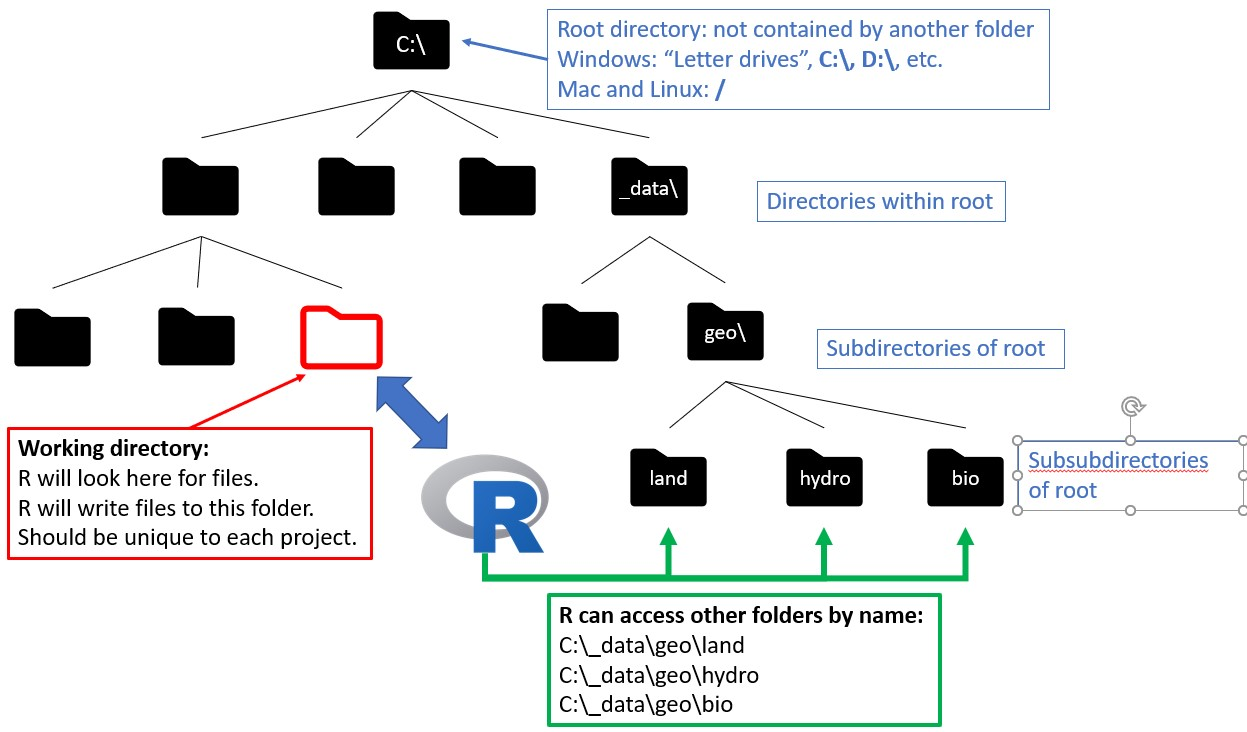
\includegraphics[keepaspectratio]{chapters/../images/04_01.jpg}}

}

\end{figure}%

You can, and should, have a separate working directory for every
project. This way files stay together, and the acts of importing and
exporting files are easier.

In R, you can find your working directory in the console with
\texttt{getwd()}:

\begin{Shaded}
\begin{Highlighting}[]
\FunctionTok{getwd}\NormalTok{()}
\end{Highlighting}
\end{Shaded}

\begin{verbatim}
[1] "C:/_courses/appl-biol-data-analysis/chapters"
\end{verbatim}

You can change it with \texttt{setwd()}:

\begin{Shaded}
\begin{Highlighting}[]
\CommentTok{\# example; not run}
\FunctionTok{setwd}\NormalTok{(}\StringTok{"C:/Users/ngreen62/Documents/biol 7410"}\NormalTok{)}
\end{Highlighting}
\end{Shaded}

These commands are usually run first in a script, to facilitate data
import.

In RStudio, you can set your working directory in the Files tab by first
navigating to a folder, then clicking \textbf{More - Set as working
directory}.

\begin{figure}

\begin{minipage}[t]{0.50\linewidth}

\begin{figure}[H]

\subcaption{To set your working directory, first click on the \ldots{}
button on the right side of the Files tab.}

{\centering \pandocbounded{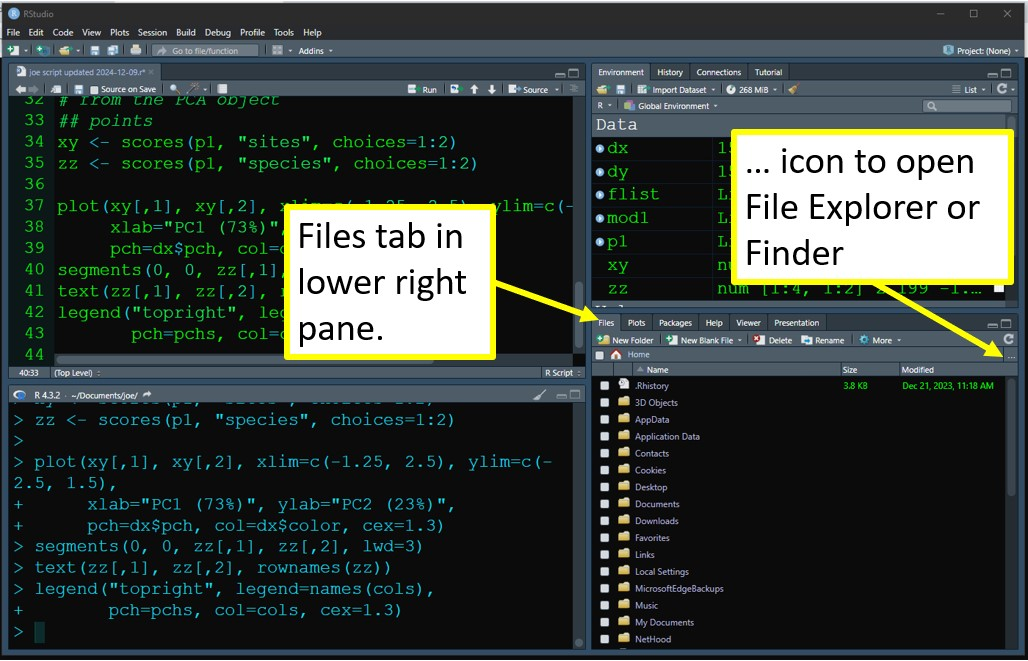
\includegraphics[keepaspectratio]{chapters/../images/04_02.jpg}}

}

\end{figure}%

\end{minipage}%
%
\begin{minipage}[t]{0.50\linewidth}

\begin{figure}[H]

\subcaption{Then, select your folder and click More\ldots Set as working
directory.}

{\centering \pandocbounded{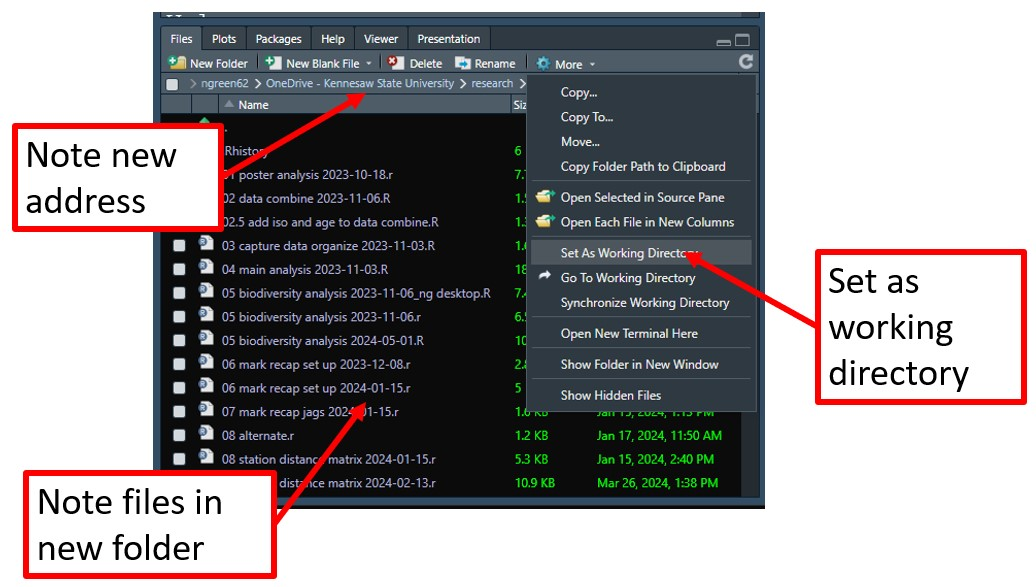
\includegraphics[keepaspectratio]{chapters/../images/04_03.jpg}}

}

\end{figure}%

\end{minipage}%

\end{figure}%

What is the advantage of setting your working directory? R will look in
the working directory \textbf{first} for any files, and put outputs
there by default.

For example, the command \texttt{dir()} lists the contents of a folder.
Without any arguments, it will automatically list the contents of the
working directory.

\begin{Shaded}
\begin{Highlighting}[]
\CommentTok{\# not run, but try on your machine:}

\CommentTok{\# equivalent commands:}
\FunctionTok{dir}\NormalTok{()}
\FunctionTok{dir}\NormalTok{(}\FunctionTok{getwd}\NormalTok{())}

\CommentTok{\# for other folders, you need to specify the path:}
\FunctionTok{dir}\NormalTok{(}\StringTok{"C:/Users/ngreen62/Documents/biol 7410/data"}\NormalTok{)}
\end{Highlighting}
\end{Shaded}

When importing data, R will import from the working directory by file
name, but requires a path for a file in any other folder.

\begin{Shaded}
\begin{Highlighting}[]
\CommentTok{\# not run}

\CommentTok{\# import from working directory:}
\NormalTok{my.data }\OtherTok{\textless{}{-}} \FunctionTok{read.csv}\NormalTok{(}\StringTok{"example.csv"}\NormalTok{)}

\CommentTok{\# equivalent: }
\NormalTok{my.data }\OtherTok{\textless{}{-}} \FunctionTok{read.csv}\NormalTok{(}\FunctionTok{paste}\NormalTok{(}\FunctionTok{getwd}\NormalTok{(), }\StringTok{"example.csv"}\NormalTok{, }\AttributeTok{sep=}\StringTok{"/"}\NormalTok{))}
\CommentTok{\# import from somewhere else:}
\NormalTok{my.data }\OtherTok{\textless{}{-}} \FunctionTok{read.csv}\NormalTok{(}\StringTok{"C:/Users/ngreen62/Documents/example.csv"}\NormalTok{)}
\end{Highlighting}
\end{Shaded}

If you open an R script with R or RStudio that is contained in a folder,
that folder will be automatically set as the working directory. Clever
use of the working directory can save you a lot of time. Sloppy use of
the working directory (e.g., not specifying the working directory in
each R or RStudio session) can lead to disaster and frustration.

\section{Formatting data files}\label{sec-ie-format}

Before you try to import your data into R, take a few minutes to set
yourself up for success.

\subsection{Naming data files}\label{sec-ie-format-name}

Good file names are essential for a working biologist. Chances are you
will work on many projects over the course of your career, each with its
own collection of data files. Even if you store each project's data in a
separate folder, it is a very good idea to give data files within those
folders names that are descriptive. I have worked with many people who
insist on using file names like ``data.xlsx'' and relying on their own
memory or paper notes to tell them which file is which. Consider this
list of particularly egregious file names:

\begin{itemize}
\item
  data.txt
\item
  Data.txt
\item
  data.set.csv
\item
  analysis data.xlsx
\item
  thesis data.xlsx
\item
  DATA FINAL - copy.txt
\item
  data current.revised.2019.txt.xlsx
\item
  final thesis data revised revised final revised analysis.csv
\end{itemize}

We are all guilty of this kind of bad naming from time to time. What do
all of the above have in common? They are vague. The names contain no
meaningful information about what the files actually contain. Some of
them are ambiguous: different operating systems or programs might read
``data.txt'' and ``Data.txt'' as the same file, or as different files!

Data file names should be short, simple, and descriptive. There are no
hard and fast rules for naming data files so I'm not going to prescribe
any. Instead, I'll share some examples and explain why these names are
helpful. As you go along and get better at working with data you will
probably develop your own habits, and that's okay. Just try to follow
the guiding principles of short, simple, and descriptive.

Here are some example file names with explanations of their desirable
properties:

\textbf{sturgeon\_growth\_data\_2017-02-21.txt}

This name declares what the file contains (growth data for sturgeon),
and the date it was created. Notice that the date is given as
``YYYY-MM-DD''. This format is useful because it automatically sorts
chronologically. This file name separates its words with underscores
rather than spaces or periods. This can prevent some occasional issues
with programs misreading file names (white space and periods can have
specific meanings in some contexts).

\textbf{dat\_combine\_2020-07-13.csv}

This name signifies that the file contains a ``combined'' dataset, and
includes the date of its creation. This would be kept in a folder with
the files that were combined to make it. Within a project I usually use
prefixes on file names to help identify them: ``dat'' for datasets with
response and explanatory variables; ``met'' for ``metadata''; ``geo'' or
``loc'' for geospatial datasets and GIS layers; and ``key'' for lookup
tables that relate dat and met files. You might develop your own
conventions for types of data that occur in your work.

\textbf{dat\_vegcover\_nrda\_releaseversion\_2021-05-03.csv}

This name is similar to the last name, but includes some additional
signifiers for the project (NRDA) and the fact that this is the final
released version.

\subsection{Setting up data files}\label{sec-ie-format-set}

Recently Broman and Woo (2018) reviewed good practices for storing data
in spreadsheets. Their article is short and easy to read, and gave a few
recommendations for data formatting:

\begin{itemize}
\item
  Be consistent
\item
  Choose good names for things
\item
  Write dates as YYYY-MM-DD
\item
  No empty cells
\item
  Put just one thing in a cell
\item
  Make it a rectangle
\item
  Create a data dictionary
\item
  No calculations in the raw data files
\item
  Do not use font color or highlighting as data
\item
  Make backups
\item
  Use data validation to avoid errors
\item
  Save the data in plain text files
\end{itemize}

Most people who work with data, myself included, probably agree with
their recommendations. Better, there is plenty of room for individual
preferences in the exact implementation of each principle. You will save
yourself a lot of headache if you follow their advice.

\subsubsection{Variable names}\label{sec-ie-format-set-vars}

Variable names, like data file names, should be brief but informative.
There are few restrictions on what variable names can be in R. For
simplicity, I recommend you use only lowercase letters, numbers,
underscores (\texttt{\_}), and periods (\texttt{.}) in variable names.
Other symbols are either inconvenient to type, or can cause issues being
parsed by R. Some common pitfalls include:

\textbf{Leading numerals} will cause an error if not enclosed in
quotation marks:

\begin{Shaded}
\begin{Highlighting}[]
\CommentTok{\# not run, but try on your machine:}

\NormalTok{x }\OtherTok{\textless{}{-}}\NormalTok{ iris[}\DecValTok{1}\SpecialCharTok{:}\DecValTok{5}\NormalTok{,]}
\FunctionTok{names}\NormalTok{(x)[}\DecValTok{1}\NormalTok{] }\OtherTok{\textless{}{-}} \StringTok{"3a"}
\NormalTok{x}\SpecialCharTok{$}\DecValTok{3}\NormalTok{a}
\NormalTok{x}\SpecialCharTok{$}\StringTok{\textquotesingle{}3a\textquotesingle{}}
\NormalTok{x[,}\StringTok{"3a"}\NormalTok{]}
\end{Highlighting}
\end{Shaded}

\textbf{Numeral-only names} will cause an error. They can also be
misinterpreted as column numbers. Don't give your variables numeral-only
names.

\begin{Shaded}
\begin{Highlighting}[]
\CommentTok{\# not run, but try on your machine:}

\NormalTok{x }\OtherTok{\textless{}{-}}\NormalTok{ iris[}\DecValTok{1}\SpecialCharTok{:}\DecValTok{5}\NormalTok{,]}
\FunctionTok{names}\NormalTok{(x)[}\DecValTok{1}\NormalTok{] }\OtherTok{\textless{}{-}} \StringTok{"3"}
\NormalTok{x}\SpecialCharTok{$}\DecValTok{3}     \CommentTok{\# error}
\NormalTok{x}\SpecialCharTok{$}\StringTok{\textquotesingle{}3\textquotesingle{}}   \CommentTok{\# works}
\NormalTok{x[,}\DecValTok{3}\NormalTok{]   }\CommentTok{\# column number 3}
\NormalTok{x[,}\StringTok{"3"}\NormalTok{] }\CommentTok{\# column named "3"}
\end{Highlighting}
\end{Shaded}

\textbf{Spaces} in variable names will cause errors because R interprets
a space as whitespace, not part of a name. If you insist on using
spaces, enclose the variable name in quotation marks every time you use
it. This is one of the few places where R cares about whitespace.

\begin{Shaded}
\begin{Highlighting}[]
\CommentTok{\# not run, but try on your machine:}

\NormalTok{x }\OtherTok{\textless{}{-}}\NormalTok{ iris[}\DecValTok{1}\SpecialCharTok{:}\DecValTok{5}\NormalTok{,]}
\FunctionTok{names}\NormalTok{(x)[}\DecValTok{1}\NormalTok{] }\OtherTok{\textless{}{-}} \StringTok{"a b"}

\CommentTok{\# causes error:}
\NormalTok{x}\SpecialCharTok{$}\NormalTok{a b}

\CommentTok{\# works:}
\NormalTok{x}\SpecialCharTok{$}\StringTok{\textquotesingle{}a b\textquotesingle{}}
\end{Highlighting}
\end{Shaded}

\textbf{Special characters} in variable names can cause issues with
parsing. Many symbols that you might think to use, such as hyphens (aka:
dashes, -) or slashes / are also R operators. Again, try to avoid these
issues by using only letters, numbers, underscores, and periods.

\begin{Shaded}
\begin{Highlighting}[]
\CommentTok{\# not run, but try on your machine:}

\NormalTok{x }\OtherTok{\textless{}{-}}\NormalTok{ iris[}\DecValTok{1}\SpecialCharTok{:}\DecValTok{5}\NormalTok{,]}
\FunctionTok{names}\NormalTok{(x)[}\DecValTok{1}\NormalTok{] }\OtherTok{\textless{}{-}} \StringTok{"a/b"}
\NormalTok{b }\OtherTok{\textless{}{-}} \DecValTok{10}
\CommentTok{\# error:}
\NormalTok{x}\SpecialCharTok{$}\NormalTok{a}\SpecialCharTok{/}\NormalTok{b}
\CommentTok{\# works:}
\NormalTok{x}\SpecialCharTok{$}\StringTok{\textquotesingle{}a/b\textquotesingle{}}

\FunctionTok{names}\NormalTok{(x)[}\DecValTok{1}\NormalTok{] }\OtherTok{\textless{}{-}} \StringTok{"surv\%"}
\NormalTok{x}
\CommentTok{\# error:}
\NormalTok{x}\SpecialCharTok{$}\NormalTok{surv\%}

\CommentTok{\# works:}
\NormalTok{x}\SpecialCharTok{$}\StringTok{\textquotesingle{}surv\%\textquotesingle{}}
\end{Highlighting}
\end{Shaded}

\textbf{Uppercase letters} in variable names work just fine, but they
can be inconvenient. Because R is case sensitive, you need to type the
variable exactly the same way each time. This can be tedious if you have
several variables with similar names. In my code I prefer to use only
lower case letters, so I don't ever have to remember how names are
capitalized.

\begin{Shaded}
\begin{Highlighting}[]
\NormalTok{x }\OtherTok{\textless{}{-}}\NormalTok{ iris[}\DecValTok{1}\SpecialCharTok{:}\DecValTok{5}\NormalTok{,]}
\FunctionTok{names}\NormalTok{(x)[}\DecValTok{1}\NormalTok{] }\OtherTok{\textless{}{-}} \StringTok{"sep.len"} \CommentTok{\# convenient}
\FunctionTok{names}\NormalTok{(x)[}\DecValTok{2}\NormalTok{] }\OtherTok{\textless{}{-}} \StringTok{"SEP.LEN"} \CommentTok{\# slightly inconvenient}
\FunctionTok{names}\NormalTok{(x)[}\DecValTok{3}\NormalTok{] }\OtherTok{\textless{}{-}} \StringTok{"Sep.Len"} \CommentTok{\# more inconvenient}
\FunctionTok{names}\NormalTok{(x)[}\DecValTok{4}\NormalTok{] }\OtherTok{\textless{}{-}} \StringTok{"SeP.lEn"} \CommentTok{\# just don\textquotesingle{}t}
\NormalTok{x}
\DocumentationTok{\#\#   sep.len SEP.LEN Sep.Len SeP.lEn Species}
\DocumentationTok{\#\# 1     5.1     3.5     1.4     0.2  setosa}
\DocumentationTok{\#\# 2     4.9     3.0     1.4     0.2  setosa}
\DocumentationTok{\#\# 3     4.7     3.2     1.3     0.2  setosa}
\DocumentationTok{\#\# 4     4.6     3.1     1.5     0.2  setosa}
\DocumentationTok{\#\# 5     5.0     3.6     1.4     0.2  setosa}
\end{Highlighting}
\end{Shaded}

\subsubsection{Data values}\label{sec-ie-format-set-vars-values}

All data in R have a type: numeric, logical, character, etc., as we
learned in Section~\ref{sec-object-type}. Within a vector, matrix, or
array, all values must have the same type or they will be converted to
character strings. Each variable in a data frame (the most common R data
structure) is essentially a vector. This means that in your input file
you should try to have one and only one type of data in each column.
Otherwise, R will coerce the values into character strings, which may or
may not be a problem. Putting only one type of value into each column
will also help get your data into ``wide'' or ``tidy'' format (Wickham
2014).

Entering data should also include some measure of \textbf{quality
assurance and quality control (QA/QC)}. This basically means making sure
that your data are entered correctly, and are formatted correctly.
Correct entry can be accomplished by direct comparison to original
datasheets or lab notebooks. Cross-checking is a valuable tool here:
have two people enter the data and compare their files.

Data formatting requires thinking about what kinds of data are being
entered. For numbers, this means entering the correct values and an
appropriate number of significant digits. For text values, this may mean
spell-checking or settling on a standard set of possible values. The
figure below shows some problems that a QA/QC step might fix:

\begin{figure}[H]

\caption{Examples of bad data management that some simple QA/QC might
fix.}

{\centering \pandocbounded{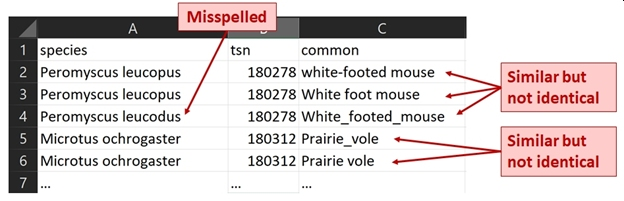
\includegraphics[keepaspectratio]{chapters/../images/04_04.jpg}}

}

\end{figure}%

\section{Data import}\label{sec-ie-import}

\subsection{Importing from text files}\label{sec-ie-import-text}

\subsubsection{Importing from the working
directory}\label{importing-from-the-working-directory}

Data for R should be stored in plain-text files. Two of the most popular
options are tab-delimited files (\textbf{.txt}) and comma-delimited
files (\textbf{.csv}). The ``delimited'' part means that some special
character (like tab or comma) is used to separate values on a row of the
file. Text files can be produced from Excel spreadsheets by going to
\textbf{Save as}, selecting a folder, and then selecting ``Text (Tab
delimited)(*.txt)'' or ``CSV (Comma delimited)(*.csv)'' from the
dropdown menu for file type. Do \textbf{\emph{not}} select ``CSV UTF-8
(Comma delimited)(*.csv)'' as this will cause issues in R.

Download the files neon\_taxa\_2025-08-03.txt and
neon\_taxa\_2025-08-03.csv. Create a new folder for this exercise, save
both files there, and set that folder as your R working directory before
continuing.

Use \texttt{read.table()} to import a tab-delimited file, and save it to
an object called \texttt{dx}. Notice that the filename must be spelled
and capitalized correctly. Notice also that because the file is in your
working directory, no folder path is needed. The argument
\texttt{header=TRUE} tells R that the first row of the file contains
column names, not data.

\begin{Shaded}
\begin{Highlighting}[]
\NormalTok{dx }\OtherTok{\textless{}{-}} \FunctionTok{read.table}\NormalTok{(}\StringTok{"neon\_taxa\_2025{-}08{-}03.txt"}\NormalTok{, }\AttributeTok{header=}\ConstantTok{TRUE}\NormalTok{)}
\end{Highlighting}
\end{Shaded}

Use \texttt{read.csv()} to import a comma-delimited file. Note how
similar the syntax is to the first command, except that for
\texttt{read.csv()} you don't need \texttt{header=TRUE} because this is
the default (unlike \texttt{read.table()}).

\begin{Shaded}
\begin{Highlighting}[]
\NormalTok{dx }\OtherTok{\textless{}{-}} \FunctionTok{read.csv}\NormalTok{(}\StringTok{"neon\_taxa\_2025{-}08{-}03.csv"}\NormalTok{, }\AttributeTok{header=}\ConstantTok{TRUE}\NormalTok{)}
\end{Highlighting}
\end{Shaded}

While \texttt{read.table()} imports tab-delimited files by default, it
can also import other types of files by setting the \texttt{sep}
argument. Below is an example of using \texttt{read.table()} to import a
CSV file.

\begin{Shaded}
\begin{Highlighting}[]
\NormalTok{dat }\OtherTok{\textless{}{-}} \FunctionTok{read.table}\NormalTok{(}\StringTok{"neon\_taxa\_2025{-}08{-}03.csv"}\NormalTok{,}
    \AttributeTok{header=}\ConstantTok{TRUE}\NormalTok{, }\AttributeTok{sep=}\StringTok{","}\NormalTok{)}
\end{Highlighting}
\end{Shaded}

\subsubsection{Importing from another
folder}\label{importing-from-another-folder}

Working from the working directory is often quick and convenient, but if
your data files are in different folders it can be awkward and
time-consuming to continually change the working directory. Instead, you
can skip the working directory and specify folders directly.

Imagine you have data files spread across 2 folders, ``capture'' and
``geo'', which are both contained by another folder ``\_data''. You can
combine folder names together in R with the \texttt{paste()} command.
This command concatenates, or sticks together, character strings.
Separating folder names from file names also makes your code more
portable. For example, if you move your data to another server or drive,
you could only have to change one line of code (provided that you
maintain the directory structure that it contains).

Consider this example. In most of my projects I call datasets from
multiple locations (because I use many common data files that are too
large to make copies of in project-specific directories), so this is how
I structure data import:

\begin{Shaded}
\begin{Highlighting}[]
\CommentTok{\# Not run; for illustration purposes only}

\CommentTok{\# directory that contains everything}
\NormalTok{top.dir }\OtherTok{\textless{}{-}} \StringTok{"K:/\_data"}

\CommentTok{\# folder that contains the capture data}
\NormalTok{cap.dir }\OtherTok{\textless{}{-}} \StringTok{"capture"}

\CommentTok{\# folder that contains geospatial data}
\NormalTok{geo.dir }\OtherTok{\textless{}{-}} \StringTok{"geo"}

\CommentTok{\# import something from capture}
\NormalTok{in.fold }\OtherTok{\textless{}{-}} \FunctionTok{paste}\NormalTok{(top.dir, cap.dir, }\AttributeTok{sep=}\StringTok{"/"}\NormalTok{)}
\NormalTok{in.name }\OtherTok{\textless{}{-}} \StringTok{"capture\_data.csv"}
\NormalTok{in.path }\OtherTok{\textless{}{-}} \FunctionTok{paste}\NormalTok{(in.fold, in.name, }\AttributeTok{sep=}\StringTok{"/"}\NormalTok{)}
\NormalTok{dx }\OtherTok{\textless{}{-}} \FunctionTok{read.csv}\NormalTok{(in.path)}

\CommentTok{\# import something from geospatial folder}
\NormalTok{in.fold }\OtherTok{\textless{}{-}} \FunctionTok{paste}\NormalTok{(top.dir, cap.dir, }\AttributeTok{sep=}\StringTok{"/"}\NormalTok{)}
\NormalTok{in.name }\OtherTok{\textless{}{-}} \StringTok{"site\_coords.csv"}
\NormalTok{in.path }\OtherTok{\textless{}{-}} \FunctionTok{paste}\NormalTok{(in.fold, in.name, }\AttributeTok{sep=}\StringTok{"/"}\NormalTok{)}
\NormalTok{cx }\OtherTok{\textless{}{-}} \FunctionTok{read.csv}\NormalTok{(in.path)}
\end{Highlighting}
\end{Shaded}

\subsubsection{\texorpdfstring{Arguments to \texttt{read.table()} and
\texttt{read.csv()}}{Arguments to read.table() and read.csv()}}\label{sec-ie-import-text-args}

The text file reading functions have a lot of options, but there are a
few that I find very useful (in addition to \texttt{header} above).

\paragraph{\texorpdfstring{\texttt{sep}}{sep}}\label{sep}

As seen in one of the examples above, the \texttt{sep} argument
specifies what character separates values on each line of the data file.
This argument has some useful default values. If you are using
\texttt{read.table()} with a tab-delimited file, or \texttt{read.csv()}
with a comma-delimited file, you don't need to set sep.

The default in \texttt{read.table()} reads any white space as a
delimiter. This is fine if you have a tab-delimited file, but if the
file contains a mix of spaces and tabs you might have some problems. For
example, if entries are separated by tabs, but some values contain
spaces. In those cases, specify the appropriate delimiter:

\begin{Shaded}
\begin{Highlighting}[]
\CommentTok{\# not run:}
\CommentTok{\# file is in working directory}
\NormalTok{in.name }\OtherTok{\textless{}{-}} \StringTok{"neon\_taxa\_2025{-}08{-}03.txt"}

\CommentTok{\# tab{-}delimited (sep="\textbackslash{}t"):}
\NormalTok{dat }\OtherTok{\textless{}{-}} \FunctionTok{read.table}\NormalTok{(in.name, }\AttributeTok{header=}\ConstantTok{TRUE}\NormalTok{, }\AttributeTok{sep=}\StringTok{"}\SpecialCharTok{\textbackslash{}t}\StringTok{"}\NormalTok{)}

\CommentTok{\# space{-}delimited (sep=" "): }
\NormalTok{dat }\OtherTok{\textless{}{-}} \FunctionTok{read.table}\NormalTok{(in.name, }\AttributeTok{header=}\ConstantTok{TRUE}\NormalTok{, }\AttributeTok{sep=}\StringTok{" "}\NormalTok{)}
\end{Highlighting}
\end{Shaded}

The \texttt{sep} argument is usually necessary when using the
``clipboard trick'' (see Section~\ref{sec-ie-import-special})

\paragraph{\texorpdfstring{\texttt{row.names}}{row.names}}\label{row.names}

When R imports a table of data, it will assign names to the rows. The
default names are just the row numbers. Some data files will have their
own row names. If you want to not import these names, you can set
row.names argument to FALSE to get the default numbers. You can also
specify names to assign upon import as a character vector.

\begin{Shaded}
\begin{Highlighting}[]
\CommentTok{\# not run:}

\CommentTok{\# make rownames "row\_1", "row\_2", and so on}
\NormalTok{use.rownames }\OtherTok{\textless{}{-}} \FunctionTok{paste}\NormalTok{(}\StringTok{"row"}\NormalTok{, }\DecValTok{1}\SpecialCharTok{:}\DecValTok{20}\NormalTok{, }\AttributeTok{sep=}\StringTok{"\_"}\NormalTok{)}
\NormalTok{dat }\OtherTok{\textless{}{-}} \FunctionTok{read.table}\NormalTok{(in.name, }\AttributeTok{header=}\ConstantTok{TRUE}\NormalTok{, }\AttributeTok{row.names=}\NormalTok{use.rownames)}
\NormalTok{dat}
\end{Highlighting}
\end{Shaded}

\paragraph{\texorpdfstring{\texttt{skip}}{skip}}\label{skip}

Some data files will contain rows of text or other information before
the tabular data starts. The argument \texttt{skip} allows you to skip
these lines. Without \texttt{skip}, R will try to read those rows of
text as if they were data and fail to import. For example, 5 rows of
preliminary text could be skipped with the argument \texttt{skip=5}.

If your data file has non-tabular header rows, the error message that
\texttt{skip} will prevent can be frustrating if you don't understand
how R parses text files. What is happening is that R uses the number of
elements in the first row to calculate the dimensions of the data frame
that it makes upon import. For example, if a text file contains the line
``These are data from Nobody (2020)'' on the first line, followed by the
tabular data, R would assume that the table contained 6 columns headed
by ``These'', ``are'', ``data'', and so on. But, if the table contained
another number of columns, R would return an error.

Why does this issue vex so many new R users (and experienced R users)?
Often we will have incomplete records in a data set, where a row is
missing values in one or more columns. Sometimes blank values are not
read correctly.

There are a few ways to deal with the errors caused by blanks. The first
is to go back to the original datafile and put R's blank value,
\texttt{NA}, in the blanks. You could also put in a value that is not
likely to occur, such as \texttt{-9999} in variables that must be
positive. This would make your file more readable, but without locking
you in to using R. Either solution will ensure that missing values are
not interpreted as extra white space. This method can be very time
consuming for very large datasets, even in Excel (or especially in
Excel). The best time to fix this issue is at data entry. Recall that
having no empty cells is one of the recommendations of Broman and Woo
(2018).

Another way is to save the file as a comma-delimited file, because
commas are less ambiguous than white space for defining missing values.
This method usually works, but might still create problems if there are
multiple blank values per record or blanks at the ends of rows. The
third option is to use the \texttt{fill} argument in the R import
functions (see below).

\paragraph{\texorpdfstring{\texttt{fill}}{fill}}\label{fill}

As described above, missing values can cause problems when importing
data into R. One way to deal with missing values that occur at the end
of a line in the data file is to use the fill argument. Setting
\texttt{fill=TRUE} will automatically pad the data frame with blanks so
that every row has the same number of values.

As convenient as \texttt{fill=TRUE} can be, you need to be careful when
using it. R may add the wrong number of values, or values of the wrong
type. One common mistake is for a blank character string (\texttt{""})
to be put in place of a missing value \texttt{NA}. This is an important
difference because \texttt{""} and \texttt{NA} are treated very
differently by many R functions.

\paragraph{\texorpdfstring{\texttt{stringsAsFactors}}{stringsAsFactors}}\label{stringsasfactors}

A \textbf{factor} is a variable in a dataset that defines group
membership: control vs.~treated, red vs.~blue, gene 1 vs.~gene 2
vs.~gene 3, and so on. The different groups to which an observation can
belong are called the \textbf{levels} of the factor. This is very useful
for statistical modeling, but can be a pain in the neck when trying to
work with data in R.

Functions \texttt{read.table()} and \texttt{read.csv()} have an argument
to automatically convert character strings to factors for convenience:
\texttt{stringsAsFactors}. This is a logical switch that will interpret
character strings as levels of a factor (\texttt{stringsAsFactors=TRUE})
or as character strings (\texttt{stringsAsFactors=FALSE}). The default
was \texttt{TRUE} until around version 4.0 or so, but now the default is
the much more convenient \texttt{FALSE}.

The reason that factors can cause headaches in R is because although
they look like character strings, they are really numeric codes and the
text you see is just a label. If you try to use a factor as if it was a
character string, you can get strange errors. My advice is to always
import data with \texttt{stringsAsFactors=FALSE} and only convert to
factor later if needed. Most statistical functions will convert to
factor for you automatically anyway. The only time when you may want to
store data as a factor is when you a very large dataset with many levels
of a factor; in those situations, factors will use memory more
efficiently.

If you get tired of typing \texttt{stringsAsFactors=TRUE} in your import
commands, you can set an option at the beginning of your script that
will change the default behavior of \texttt{read.table()} and
\texttt{read.csv()}:

\begin{Shaded}
\begin{Highlighting}[]
\CommentTok{\# not run}
\FunctionTok{options}\NormalTok{(}\AttributeTok{stringsAsFactors=}\ConstantTok{FALSE}\NormalTok{)}
\end{Highlighting}
\end{Shaded}

Back when this option was \texttt{TRUE} by default I put this command at
the start of every new R script to avoid problems with text strings
being misinterpreted as factors.

\subsection{Saving and importing R objects}\label{sec-ie-import-object}

Some R objects are not easily represented by tables. For example, the
outputs of statistical methods are usually \textbf{lists}. Such objects
can be saved using function \texttt{saveRDS()} and read into R using
\texttt{readRDS()}. The example below will save an R data object to file
\texttt{rds\_test.rds} in your R working directory.

\begin{Shaded}
\begin{Highlighting}[]
\CommentTok{\# fit a linear model and save its output}
\CommentTok{\# as an R object (list)}
\NormalTok{mod1 }\OtherTok{\textless{}{-}} \FunctionTok{lm}\NormalTok{(Petal.Width}\SpecialCharTok{\textasciitilde{}}\NormalTok{Sepal.Width, }\AttributeTok{data=}\NormalTok{iris)}
\NormalTok{mod1}
\DocumentationTok{\#\# }
\DocumentationTok{\#\# Call:}
\DocumentationTok{\#\# lm(formula = Petal.Width \textasciitilde{} Sepal.Width, data = iris)}
\DocumentationTok{\#\# }
\DocumentationTok{\#\# Coefficients:}
\DocumentationTok{\#\# (Intercept)  Sepal.Width  }
\DocumentationTok{\#\#      3.1569      {-}0.6403}
\FunctionTok{saveRDS}\NormalTok{(mod1, }\StringTok{"rds\_test.rds"}\NormalTok{)}
\end{Highlighting}
\end{Shaded}

\begin{Shaded}
\begin{Highlighting}[]
\CommentTok{\# now read it back in:}
\NormalTok{b }\OtherTok{\textless{}{-}} \FunctionTok{readRDS}\NormalTok{(}\StringTok{"rds\_test.rds"}\NormalTok{)}
\NormalTok{b}
\end{Highlighting}
\end{Shaded}

\begin{verbatim}

Call:
lm(formula = Petal.Width ~ Sepal.Width, data = iris)

Coefficients:
(Intercept)  Sepal.Width  
     3.1569      -0.6403  
\end{verbatim}

There is a lazier way to accomplish this task using function
\texttt{dput()}. This function saves a plain text representation of an
object that can later be used to recreate the object (i.e., R code that
can reproduce the object). The help file for \texttt{dput()} cautions
that this is not a good method for transferring objects between R
sessions and recommends using \texttt{saveRDS()} instead. That being
said, I've used this method for years and have never had a problem. The
procedure is to copy the output of \texttt{dput()} into your R script,
and later assign that text to another object. Use \texttt{dput()} at
your own risk.

\begin{Shaded}
\begin{Highlighting}[]
\NormalTok{a }\OtherTok{\textless{}{-}}\NormalTok{ iris[}\DecValTok{1}\SpecialCharTok{:}\DecValTok{6}\NormalTok{,]}
\FunctionTok{dput}\NormalTok{(a)}
\end{Highlighting}
\end{Shaded}

\begin{verbatim}
structure(list(Sepal.Length = c(5.1, 4.9, 4.7, 4.6, 5, 5.4), 
    Sepal.Width = c(3.5, 3, 3.2, 3.1, 3.6, 3.9), Petal.Length = c(1.4, 
    1.4, 1.3, 1.5, 1.4, 1.7), Petal.Width = c(0.2, 0.2, 0.2, 
    0.2, 0.2, 0.4), Species = structure(c(1L, 1L, 1L, 1L, 1L, 
    1L), levels = c("setosa", "versicolor", "virginica"), class = "factor")), row.names = c(NA, 
6L), class = "data.frame")
\end{verbatim}

\subsection{Importing from saved workspaces}\label{sec-ie-import-rdata}

Everything you do in R takes place within the \textbf{workspace}. This
can be thought of as a sandbox where all of your data and functions
reside. If you want to save this entire environment and continue working
later you can do this by saving the workspace with \texttt{save.image()}
(see Section~\ref{sec-ie-export-rdata}).

Workspaces can be loaded using function \texttt{load()}. The example
below loads workspace \texttt{example.RData} from your home directory.
Notice that this command will load every object from the saved workspace
into your current workspace. This might cause problems if the saved
workspace and current workspace have objects with the same names.

\begin{Shaded}
\begin{Highlighting}[]
\CommentTok{\# not run:}
\FunctionTok{load}\NormalTok{(}\StringTok{"example.RData"}\NormalTok{)}
\end{Highlighting}
\end{Shaded}

When loading a workspace, it is sometimes more useful to import it into
a new \textbf{environment}. An environment is like a container within
your workspace that contain objects that arent' visible to the outer
workspace. In other words, you can import objects from that workspace
without putting all of its objects into your current workspace. I use
this method a lot for working with large sets of model outputs. The
typical workflow is:

\begin{enumerate}
\def\labelenumi{\arabic{enumi}.}
\tightlist
\item
  Run an analysis or set of simulations in multiple R instances and save
  the results of each in its own R workspace.
\item
  After simulations are complete, import the results of each simulation
  from its individual workspace into a new environment.
\item
  Copy the objects from the environment containing the loaded workspace
  to the main workspace.
\item
  Delete the environment containing the loaded workspace.
\item
  Repeat until all results are imported.
\end{enumerate}

Here is an example of importing individual objects from a workspace into
a new environment, then copying that object into the current workspace:

\begin{Shaded}
\begin{Highlighting}[]
\CommentTok{\# not run:}
\FunctionTok{rm}\NormalTok{(a) }\CommentTok{\# will return error if a does not already exist}

\CommentTok{\# set up a new environment}
\NormalTok{temp }\OtherTok{\textless{}{-}} \FunctionTok{new.env}\NormalTok{()}

\CommentTok{\# load the previously saved workspace}
\CommentTok{\# into the new environment}
\FunctionTok{load}\NormalTok{(}\StringTok{"example.RData"}\NormalTok{, }\AttributeTok{env=}\NormalTok{temp)}

\CommentTok{\# access an object called "a" from the }
\CommentTok{\# imported workspace. Note that a will}
\CommentTok{\# not be available from outside temp.}
\NormalTok{a }\OtherTok{\textless{}{-}}\NormalTok{ temp}\SpecialCharTok{$}\NormalTok{a}

\CommentTok{\# remove the container; create a new one}
\CommentTok{\# for the next import or step of the loop}
\FunctionTok{rm}\NormalTok{(temp)}

\CommentTok{\# inspect your imported object}
\NormalTok{a}
\end{Highlighting}
\end{Shaded}

\subsection{Importing special cases}\label{sec-ie-import-special}

\subsubsection{The clipboard trick}\label{sec-ie-import-special-clip}

Sometimes it can be convenient to copy and paste data directly from a
spreadsheet into R. This is fine for quick or one-off data imports, but
not recommended for routine use because it is tedious to reproduce and
error-prone. The procedure is as follows:

\begin{enumerate}
\def\labelenumi{\arabic{enumi}.}
\tightlist
\item
  In the R console, type this command but do NOT run it:
  \texttt{a\ \textless{}-\ read.table("clipboard",\ header=TRUE,\ sep="\textbackslash{}t")}
\item
  In Excel, highlight your data and copy it to the clipboard using
  Ctrl-C (or Cmd-C on a Mac).
\item
  Click in the R console to move your focus there. In R, hit the ENTER
  key.
\item
  The command you typed--but did not execute--in step 1 will read the
  table from the clipboard.
\end{enumerate}

Note that if you try to copy/paste the
\texttt{read.table("clipboard",...)} command into the R console, you
will then have that command in your clipboard and not your data.

\subsubsection{\texorpdfstring{Entering data using
\texttt{scan()}}{Entering data using scan()}}\label{sec-ie-import-special-scan}

The \texttt{scan()} function lets you enter values one-by-one, separated
by pressing ENTER. You can use this just like typing values into Excel.
Or, you can copy and paste a single column of values from Excel. The
latter case works because R interprets the values within a column as
being separated by a line return (i.e., pressing ENTER).

Type the name of an object to which data will be saved, the assignment
operator \texttt{\textless{}-}, \texttt{scan()}, then ENTER, then values
(each followed by ENTER), then hit ENTER twice after the last value.
This is obviously inefficient for large datasets, but it's a nice trick
to be aware of.

\begin{Shaded}
\begin{Highlighting}[]
\CommentTok{\# Not run, but try on your machine.}

\NormalTok{a }\OtherTok{\textless{}{-}} \FunctionTok{scan}\NormalTok{()}
\DecValTok{1}
\DecValTok{2}
\DecValTok{3}
\DecValTok{4}
\DecValTok{5}


\NormalTok{a}
\end{Highlighting}
\end{Shaded}

You can use this function to enter values from a column in Excel,
highlight and copy the column. Then go to R, enter the command below,
and press ENTER. Then paste your values and press ENTER again.

\subsubsection{\texorpdfstring{Entering data directl using
\texttt{c()}}{Entering data directl using c()}}\label{sec-ie-import-special-c}

Function \texttt{c()} combines its arguments as a vector. As with all
functions, arguments must be separated by commas. Arguments can be on
the same line or on different lines.

\begin{Shaded}
\begin{Highlighting}[]

\FunctionTok{c}\NormalTok{(}\DecValTok{1}\SpecialCharTok{:}\DecValTok{3}\NormalTok{,}\DecValTok{9}\SpecialCharTok{:}\DecValTok{5}\NormalTok{)}
\DocumentationTok{\#\# [1] 1 2 3 9 8 7 6 5}

\NormalTok{a }\OtherTok{\textless{}{-}} \FunctionTok{c}\NormalTok{(}\DecValTok{1}\NormalTok{,}
      \DecValTok{3}\NormalTok{,}
       \DecValTok{5}
\NormalTok{       )}
\NormalTok{a}
\DocumentationTok{\#\# [1] 1 3 5}
\end{Highlighting}
\end{Shaded}

Like \texttt{scan()}, data can be entered directly into the console
using \texttt{c()}. Also like \texttt{scan()}, this is comically
inefficient but can be useful for small numbers of values.

\section{Data export}\label{sec-ie-export}

\subsection{Exporting text files}\label{sec-ie-export-text}

Everything you do in R takes place within the ``workspace''. You can
save entire workspaces, but in most situations it is more useful to
write out data or results as delimited text files. I've found that
comma-delimited files are slightly less likely to have issues because
they use a character (\texttt{,}) rather than whitespace to separate
values. So, for the rest of this course we'll use CSV files.

Tab-delimited files are written out using \texttt{write.table()}. In the
example below, the first argument \texttt{dat} is the object from the R
workspace that you want to write out. The argument \texttt{sep} works
the same way as in \texttt{read.table()}. The example below will save a
file called \texttt{mydata.txt} in working directory. Option
\texttt{sep="\textbackslash{}\textbackslash{}t"} can be provided to
ensure that the file is written as a tab-delimited file and not a
space-delimited file.

\begin{Shaded}
\begin{Highlighting}[]
\CommentTok{\# not run:}
\NormalTok{dat }\OtherTok{\textless{}{-}}\NormalTok{ iris[}\DecValTok{1}\SpecialCharTok{:}\DecValTok{6}\NormalTok{,]}
\FunctionTok{write.table}\NormalTok{(dat,}\StringTok{"mydata.txt"}\NormalTok{, }\AttributeTok{sep=}\StringTok{"}\SpecialCharTok{\textbackslash{}t}\StringTok{"}\NormalTok{)}
\end{Highlighting}
\end{Shaded}

Comma-delimited files are written out by \texttt{write.csv()}. The
syntax is similar to \texttt{write.table()}. Note that the file
extension must be ``.csv'' instead of ``.txt''. If you save a file with
the wrong extension, then it may be corrupt or unusable (or, R might
return an error).

\begin{Shaded}
\begin{Highlighting}[]
\CommentTok{\# not run:}
\FunctionTok{write.csv}\NormalTok{(dat,}\StringTok{"mydata.csv"}\NormalTok{)}
\end{Highlighting}
\end{Shaded}

Most of the time you will not be saving files to your home directory,
but to another folder. The folder and the file name must both be
specified to save somewhere else. It is usually a good idea to define
the file name and file destination separately. This way if you re-use
your code on another machine, or a different folder, you only need to
update the folder address once.

\begin{Shaded}
\begin{Highlighting}[]
\CommentTok{\# not run:}

\CommentTok{\# do this:}
\NormalTok{out.dir }\OtherTok{\textless{}{-}} \StringTok{"C:/\_data"}
\NormalTok{out.name }\OtherTok{\textless{}{-}} \StringTok{"mydata.csv"}
\FunctionTok{write.csv}\NormalTok{(dat, }\FunctionTok{paste}\NormalTok{(out.dir, out.name, }\AttributeTok{sep=}\StringTok{"/"}\NormalTok{))}

\CommentTok{\# or this:}
\NormalTok{out.dir }\OtherTok{\textless{}{-}} \StringTok{"C:/\_data"}
\NormalTok{out.name }\OtherTok{\textless{}{-}} \StringTok{"mydata.csv"}
\NormalTok{out.path }\OtherTok{\textless{}{-}} \FunctionTok{paste}\NormalTok{(out.dir, out.name, }\AttributeTok{sep=}\StringTok{"/"}\NormalTok{)}
\FunctionTok{write.csv}\NormalTok{(dat, out.path)}

\CommentTok{\# not this:}
\FunctionTok{write.csv}\NormalTok{(dat, }\StringTok{"C:/\_data/mydata.csv"}\NormalTok{)}
\end{Highlighting}
\end{Shaded}

The last example is problematic because the output file name contains
both the destination folder and the filename itself. If you try to run
your code on another machine, it will take longer to update the code
with a new folder address. This method is also problematic because
exporting multiple files will require typing the folder address multiple
times. Consider this example:

\begin{Shaded}
\begin{Highlighting}[]
\CommentTok{\# not run:}

\NormalTok{dat1 }\OtherTok{\textless{}{-}}\NormalTok{ iris[}\DecValTok{1}\SpecialCharTok{:}\DecValTok{6}\NormalTok{,]}
\NormalTok{dat2 }\OtherTok{\textless{}{-}}\NormalTok{ iris[}\DecValTok{7}\SpecialCharTok{:}\DecValTok{12}\NormalTok{,]}

\FunctionTok{write.csv}\NormalTok{(dat1, }\StringTok{"C:/\_data/mydata1.csv"}\NormalTok{)}
\FunctionTok{write.csv}\NormalTok{(dat2, }\StringTok{"C:/\_data/mydata2.csv"}\NormalTok{)}
\end{Highlighting}
\end{Shaded}

Running that code on a new machine, or modifying it for a new project in
a different folder, requires changing the folder address twice. The
better way is to define the folder name only once:

\begin{Shaded}
\begin{Highlighting}[]
\CommentTok{\# not run:}

\NormalTok{out.dir }\OtherTok{\textless{}{-}} \StringTok{"C:/\_data"}
\FunctionTok{write.csv}\NormalTok{(dat1, }\FunctionTok{paste}\NormalTok{(out.dir, }\StringTok{"mydata1.csv"}\NormalTok{, }\AttributeTok{sep=}\StringTok{"/"}\NormalTok{))}
\FunctionTok{write.csv}\NormalTok{(dat2, }\FunctionTok{paste}\NormalTok{(out.dir, }\StringTok{"mydata2.csv"}\NormalTok{, }\AttributeTok{sep=}\StringTok{"/"}\NormalTok{))}
\end{Highlighting}
\end{Shaded}

See the difference? The revised code is much more portable and reusable.
This illustrates a good practice for programming in general (not just R)
called \textbf{``Single Point of Definition''}. Defining variables or
objects once and only once makes your code more robust to changes and
easier to maintain or reuse. The example below shows a more compact way
to export the files \texttt{mydata1.csv} and \texttt{mydata2.csv}, with
even fewer points of definition for file names:

\begin{Shaded}
\begin{Highlighting}[]
\CommentTok{\# not run:}

\NormalTok{out.dir }\OtherTok{\textless{}{-}} \StringTok{"C:/\_data"}
\NormalTok{out.names }\OtherTok{\textless{}{-}} \FunctionTok{paste0}\NormalTok{(}\StringTok{"mydata"}\NormalTok{, }\DecValTok{1}\SpecialCharTok{:}\DecValTok{2}\NormalTok{, }\StringTok{".csv"}\NormalTok{)}
\NormalTok{out.files }\OtherTok{\textless{}{-}} \FunctionTok{paste}\NormalTok{(out.dir, out.names, }\AttributeTok{sep=}\StringTok{"/"}\NormalTok{)}
\FunctionTok{write.csv}\NormalTok{(dat1, out.files[}\DecValTok{1}\NormalTok{])}
\FunctionTok{write.csv}\NormalTok{(dat2, out.files[}\DecValTok{2}\NormalTok{])}
\end{Highlighting}
\end{Shaded}

One handy trick is to auto-generate an output filename that includes the
current date. This can really help keep multiple versions of analyses or
model runs organized. The \texttt{paste0()} command pastes its arguments
together as they are, with no separator between them (equivalent to
\texttt{paste(...,sep="")}). Function \texttt{Sys.Date()} prints the
current date (according to your machine) in YYYY-MM-DD format.

\begin{Shaded}
\begin{Highlighting}[]
\CommentTok{\# not run:}

\NormalTok{out.dir }\OtherTok{\textless{}{-}} \StringTok{"C:/\_data"}
\NormalTok{out.name }\OtherTok{\textless{}{-}} \FunctionTok{paste0}\NormalTok{(}\StringTok{"mydata"}\NormalTok{, }\StringTok{"\_"}\NormalTok{, }\FunctionTok{Sys.Date}\NormalTok{(), }\StringTok{".csv"}\NormalTok{)}
\FunctionTok{write.csv}\NormalTok{(dat, }\FunctionTok{paste}\NormalTok{(out.dir, out.name, }\AttributeTok{sep=}\StringTok{"/"}\NormalTok{))}
\end{Highlighting}
\end{Shaded}

\subsection{Saving R objects}\label{sec-ie-export-robj}

Some data do not fit easily into tables. Individual R objects can be
saved to an ``.rds'' file using the function saveRDS(). This function
saves a single object that can later be loaded into another R session
with function readRDS().

\begin{Shaded}
\begin{Highlighting}[]
\CommentTok{\# not run:}

\NormalTok{x }\OtherTok{\textless{}{-}} \FunctionTok{t.test}\NormalTok{(}\FunctionTok{rnorm}\NormalTok{(}\DecValTok{100}\NormalTok{))}

\CommentTok{\# save to working directory:}
\FunctionTok{saveRDS}\NormalTok{(x, }\StringTok{"zebra.rds"}\NormalTok{)}

\CommentTok{\# load the file:}
\NormalTok{z }\OtherTok{\textless{}{-}} \FunctionTok{readRDS}\NormalTok{(}\StringTok{"zebra.rds"}\NormalTok{)}
\end{Highlighting}
\end{Shaded}

\subsection{Saving workspaces}\label{sec-ie-export-rdata}

Entire R workspaces or parts of workspaces can be saved using the
function save.image(). The command by itself will save the entire
current workspace with a generic name to the working directory. It is
more useful to save the workspace under a particular name and/or only
save specific objects.

\begin{Shaded}
\begin{Highlighting}[]
\CommentTok{\# not run:}

\CommentTok{\# save entire workspace with generic name (avoid):}
\FunctionTok{save.image}\NormalTok{()}

\CommentTok{\# save entire workspace with specific name (better):}
\FunctionTok{save.image}\NormalTok{(}\AttributeTok{file=}\StringTok{"test1.RData"}\NormalTok{)}

\CommentTok{\# save specific objects (best):}
\NormalTok{x }\OtherTok{\textless{}{-}} \FunctionTok{rnorm}\NormalTok{(}\DecValTok{100}\NormalTok{)}
\NormalTok{z }\OtherTok{\textless{}{-}} \FunctionTok{t.test}\NormalTok{(x)}
\FunctionTok{save}\NormalTok{(}\AttributeTok{list=}\FunctionTok{c}\NormalTok{(}\StringTok{"x"}\NormalTok{, }\StringTok{"z"}\NormalTok{), }\AttributeTok{file=}\StringTok{"testworkspace.RData"}\NormalTok{)}
\end{Highlighting}
\end{Shaded}

\subsection{Write text to a file (special
cases)}\label{sec-ie-export-sink}

Sometimes you need to write out data that do not fit easily into tables.
An example might be the results of a single \emph{t}-test or ANOVA. This
is also sometimes necessary when working with programs outside of R. For
example, the program JAGS requires a text file that defines the model to
be fit (see Chapter~\ref{sec-bayes}). This text file can be generated by
R, which makes your workflow simpler because you don't need to use a
separate program to store the outputs.

The function to write text files with arbitrary content (i.e., not
tables) is \texttt{sink()}. Functions \texttt{print()} and
\texttt{cat()} are also useful in conjunction with \texttt{sink()}.

\begin{itemize}
\item
  \texttt{sink()} works in pairs. The first command defines a file to
  put text into. The second command finishes the file and writes it.
\item
  \texttt{print()} prints its arguments as-is. It should produce the
  same text as running its argument in the R console.
\item
  \texttt{cat()} stands for ``concatenate and print''. Use this to
  combine expressions and then print them.
\end{itemize}

\begin{Shaded}
\begin{Highlighting}[]
\CommentTok{\# not run, but try it on your machine}

\NormalTok{my.result }\OtherTok{\textless{}{-}} \FunctionTok{t.test}\NormalTok{(}\FunctionTok{rnorm}\NormalTok{(}\DecValTok{50}\NormalTok{))}
\FunctionTok{sink}\NormalTok{(}\StringTok{"C:/\_data/myresult.txt"}\NormalTok{)}
\FunctionTok{cat}\NormalTok{(}\StringTok{"t{-}test results:"}\NormalTok{,}\StringTok{"}\SpecialCharTok{\textbackslash{}n}\StringTok{"}\NormalTok{) }\CommentTok{\#\textbackslash{}n = new line}
\FunctionTok{print}\NormalTok{(my.result)}
\FunctionTok{sink}\NormalTok{()}
\end{Highlighting}
\end{Shaded}

\subsection{Exporting graphics}\label{sec-ie-export-graphics}

Finally, at some point you will need to export R graphics. In the base R
GUI, you can right-click your image and select ``Copy as bitmap'', and
then paste it somewhere as a .jpeg. In RStudio, you can right-click and
``Save image as\ldots{}''. However, when preparing presentation or
publication quality graphs, it helps to exert more control over the
final figure with graphics functions.

R can write images in a variety of formats, including .jpeg, .png,
.tiff, and so on. The basic process is:

\begin{enumerate}
\def\labelenumi{\arabic{enumi}.}
\tightlist
\item
  Start a new graphics device using \texttt{jpeg()} or \texttt{.png} or
  whichever function is appropriate. This function will include the
  target path as an argument.
\item
  Run the code to make your plot.
\item
  Use \texttt{dev.off()} to tell R that your plot is done, and to go
  ahead and render and save it.
\end{enumerate}

Here is an example:

\begin{Shaded}
\begin{Highlighting}[]
\CommentTok{\# not run, but try on your machine}
\CommentTok{\# will put a figure in your working directory}

\FunctionTok{jpeg}\NormalTok{(}\StringTok{"example\_fig.jpg"}\NormalTok{,             }\CommentTok{\# file name}
     \AttributeTok{width=}\DecValTok{8}\NormalTok{, }\AttributeTok{height=}\DecValTok{5}\NormalTok{, }\AttributeTok{units=}\StringTok{"in"}\NormalTok{, }\CommentTok{\# dimensions}
     \AttributeTok{res=}\DecValTok{300}\NormalTok{)                       }\CommentTok{\# resolution}
\FunctionTok{hist}\NormalTok{(}\FunctionTok{rnorm}\NormalTok{(}\DecValTok{100}\NormalTok{))                    }\CommentTok{\# make plot}
\FunctionTok{dev.off}\NormalTok{()                           }\CommentTok{\# finish figure}
\end{Highlighting}
\end{Shaded}

\chapter{Data manipulation with R}\label{sec-manip}

In \#sec-r we introduced the basics of the R language and program
environment. In this module, we'll go a few steps further and get into
the finer details of \textbf{data manipulation}: the practice of
arranging, sorting, cleaning, and modifying data--and the objects that
contain data. Data manipulation is an important R skill because real
datasets usually need some fixing before they can be properly analyzed.
Data manipulation is also and essential part of R programming for tasks
other than data analysis. For example,
\href{https://doi.org/10.5066/P935Y7NO}{simulation modeling} or document
production (e.g., this website!).

\section{Making values}\label{sec-manip-make}

The typical analysis workflow in R involves importing data from text
files or other sources. Sometimes, however, it is necessary to make
values within R. This can be for a variety of reasons:

\begin{enumerate}
\def\labelenumi{\arabic{enumi}.}
\tightlist
\item
  Producing test data sets with desired distributions
\item
  Making sets of indices or look-up values to use in other functions
\item
  Modifying existing datasets
\item
  Running simulations
\item
  And many more\ldots{}
\end{enumerate}

This section demonstrates some methods for producing values--i.e.,
data--within R.

\subsection{Make arbitrary values with the c()
function}\label{sec-manip-make-c}

The function \texttt{c()} combines its arguments as a \textbf{vector}.
As with all functions, arguments must be separated by commas and can be
on different lines. This method can be used to make vectors with any set
of values.

\begin{Shaded}
\begin{Highlighting}[]
\FunctionTok{c}\NormalTok{(}\DecValTok{1}\SpecialCharTok{:}\DecValTok{3}\NormalTok{,}\DecValTok{9}\SpecialCharTok{:}\DecValTok{5}\NormalTok{)}
\end{Highlighting}
\end{Shaded}

\begin{verbatim}
[1] 1 2 3 9 8 7 6 5
\end{verbatim}

\begin{Shaded}
\begin{Highlighting}[]
\NormalTok{a }\OtherTok{\textless{}{-}} \FunctionTok{c}\NormalTok{(}\DecValTok{1}\NormalTok{,}
      \DecValTok{3}\NormalTok{,}
       \DecValTok{5}
\NormalTok{       )}
\NormalTok{a}
\end{Highlighting}
\end{Shaded}

\begin{verbatim}
[1] 1 3 5
\end{verbatim}

Like \texttt{scan()}, this is an inefficient way to make vectors but can
be useful for small numbers of values. Or, for sets of values that can't
be defined algorithmically.

\subsection{Generating sequences}\label{sec-manip-make-seq}

\subsubsection{Consecutive values with the colon :
operator}\label{sec-manip-make-seq-col}

Consecutive values can be generated using the colon operator \texttt{:}.
A command like \texttt{X:Y} will generate consecutive values from
\emph{X} to \emph{Y} in increments of 1 or -1. If \(X<Y\), the increment
is 1; if \(X>Y\), the increment is -1. The usual use case is to make
sets of consecutive integers.

\begin{Shaded}
\begin{Highlighting}[]
\CommentTok{\# Simple examples:}
\DecValTok{1}\SpecialCharTok{:}\DecValTok{10}
\end{Highlighting}
\end{Shaded}

\begin{verbatim}
 [1]  1  2  3  4  5  6  7  8  9 10
\end{verbatim}

\begin{Shaded}
\begin{Highlighting}[]
\DecValTok{5}\SpecialCharTok{:}\DecValTok{2}
\end{Highlighting}
\end{Shaded}

\begin{verbatim}
[1] 5 4 3 2
\end{verbatim}

\begin{Shaded}
\begin{Highlighting}[]
\SpecialCharTok{{-}}\DecValTok{1}\SpecialCharTok{:}\DecValTok{10}
\end{Highlighting}
\end{Shaded}

\begin{verbatim}
 [1] -1  0  1  2  3  4  5  6  7  8  9 10
\end{verbatim}

\begin{Shaded}
\begin{Highlighting}[]
\DecValTok{10}\SpecialCharTok{:{-}}\DecValTok{1}
\end{Highlighting}
\end{Shaded}

\begin{verbatim}
 [1] 10  9  8  7  6  5  4  3  2  1  0 -1
\end{verbatim}

Sometimes you may need to use parentheses to get the intended values
because of the order in which R runs operators (aka: ``operator
precedence'').

\begin{Shaded}
\begin{Highlighting}[]
\CommentTok{\# effect of parentheses (operator precedence):}
\NormalTok{a }\OtherTok{\textless{}{-}} \DecValTok{2}\SpecialCharTok{:}\DecValTok{6}
\FunctionTok{length}\NormalTok{(a)}
\end{Highlighting}
\end{Shaded}

\begin{verbatim}
[1] 5
\end{verbatim}

\begin{Shaded}
\begin{Highlighting}[]
\DecValTok{1}\SpecialCharTok{:}\DecValTok{2}\SpecialCharTok{*}\FunctionTok{length}\NormalTok{(a)}
\end{Highlighting}
\end{Shaded}

\begin{verbatim}
[1]  5 10
\end{verbatim}

\begin{Shaded}
\begin{Highlighting}[]
\DecValTok{1}\SpecialCharTok{:}\NormalTok{(}\DecValTok{2}\SpecialCharTok{*}\FunctionTok{length}\NormalTok{(a))}
\end{Highlighting}
\end{Shaded}

\begin{verbatim}
 [1]  1  2  3  4  5  6  7  8  9 10
\end{verbatim}

\emph{X} and \emph{Y} don't have to literally be numbers; they can be
variables or R expressions that evaluate to a number. Below are some
examples:

\begin{Shaded}
\begin{Highlighting}[]
\NormalTok{a }\OtherTok{\textless{}{-}} \DecValTok{2}\SpecialCharTok{:}\DecValTok{6}
\CommentTok{\# length(a) evaluates to a number (5)}
\FunctionTok{length}\NormalTok{(a)}\SpecialCharTok{:}\DecValTok{10}
\end{Highlighting}
\end{Shaded}

\begin{verbatim}
[1]  5  6  7  8  9 10
\end{verbatim}

Most people use \texttt{:} to produce sets of integers, but it can also
make non-integers. The values will be separated by 1 or -1. The first
value will be the value before the \texttt{:}. The last value might not
be the value after the \texttt{:}. It will be the value up to or before
the second number along the sequence from the first number. If the value
before the \texttt{:} is an integer, then the sequence will consist of
integers. Note that if you want a sequence that includes non-integers,
it might be safer to use \texttt{seq()} (see below).

\begin{Shaded}
\begin{Highlighting}[]
\FloatTok{2.3}\SpecialCharTok{:}\DecValTok{5}
\end{Highlighting}
\end{Shaded}

\begin{verbatim}
[1] 2.3 3.3 4.3
\end{verbatim}

\begin{Shaded}
\begin{Highlighting}[]
\DecValTok{5}\SpecialCharTok{:}\FloatTok{2.3}
\end{Highlighting}
\end{Shaded}

\begin{verbatim}
[1] 5 4 3
\end{verbatim}

\begin{Shaded}
\begin{Highlighting}[]
\FloatTok{2.7}\SpecialCharTok{:}\FloatTok{6.1}
\end{Highlighting}
\end{Shaded}

\begin{verbatim}
[1] 2.7 3.7 4.7 5.7
\end{verbatim}

\subsubsection{Regular sequences with the seq()
function}\label{sec-manip-make-seq-seq}

Function \texttt{seq()} generates regular sequences of a given length
(\texttt{length=}), or by an interval (\texttt{by=}). The command must
be supplied with a length or an interval, but not both. If you specify a
length, R will calculate the intervals for you. If you specify an
interval, R will calculate the length for you. If you specify a length
and an interval, R will return an error.

\begin{Shaded}
\begin{Highlighting}[]
\FunctionTok{seq}\NormalTok{(}\DecValTok{0}\NormalTok{,}\DecValTok{20}\NormalTok{,}\AttributeTok{by=}\FloatTok{0.5}\NormalTok{)}
\end{Highlighting}
\end{Shaded}

\begin{verbatim}
 [1]  0.0  0.5  1.0  1.5  2.0  2.5  3.0  3.5  4.0  4.5  5.0  5.5  6.0  6.5  7.0
[16]  7.5  8.0  8.5  9.0  9.5 10.0 10.5 11.0 11.5 12.0 12.5 13.0 13.5 14.0 14.5
[31] 15.0 15.5 16.0 16.5 17.0 17.5 18.0 18.5 19.0 19.5 20.0
\end{verbatim}

\begin{Shaded}
\begin{Highlighting}[]
\FunctionTok{seq}\NormalTok{(}\SpecialCharTok{{-}}\NormalTok{pi,pi,}\AttributeTok{by=}\FloatTok{0.1}\NormalTok{)}
\end{Highlighting}
\end{Shaded}

\begin{verbatim}
 [1] -3.14159265 -3.04159265 -2.94159265 -2.84159265 -2.74159265 -2.64159265
 [7] -2.54159265 -2.44159265 -2.34159265 -2.24159265 -2.14159265 -2.04159265
[13] -1.94159265 -1.84159265 -1.74159265 -1.64159265 -1.54159265 -1.44159265
[19] -1.34159265 -1.24159265 -1.14159265 -1.04159265 -0.94159265 -0.84159265
[25] -0.74159265 -0.64159265 -0.54159265 -0.44159265 -0.34159265 -0.24159265
[31] -0.14159265 -0.04159265  0.05840735  0.15840735  0.25840735  0.35840735
[37]  0.45840735  0.55840735  0.65840735  0.75840735  0.85840735  0.95840735
[43]  1.05840735  1.15840735  1.25840735  1.35840735  1.45840735  1.55840735
[49]  1.65840735  1.75840735  1.85840735  1.95840735  2.05840735  2.15840735
[55]  2.25840735  2.35840735  2.45840735  2.55840735  2.65840735  2.75840735
[61]  2.85840735  2.95840735  3.05840735
\end{verbatim}

\begin{Shaded}
\begin{Highlighting}[]
\FunctionTok{seq}\NormalTok{(}\SpecialCharTok{{-}}\DecValTok{1}\NormalTok{,}\DecValTok{1}\NormalTok{,}\AttributeTok{length=}\DecValTok{20}\NormalTok{)}
\end{Highlighting}
\end{Shaded}

\begin{verbatim}
 [1] -1.00000000 -0.89473684 -0.78947368 -0.68421053 -0.57894737 -0.47368421
 [7] -0.36842105 -0.26315789 -0.15789474 -0.05263158  0.05263158  0.15789474
[13]  0.26315789  0.36842105  0.47368421  0.57894737  0.68421053  0.78947368
[19]  0.89473684  1.00000000
\end{verbatim}

\begin{Shaded}
\begin{Highlighting}[]
\CommentTok{\# returns an error:}
\DocumentationTok{\#\# not run:}
\FunctionTok{seq}\NormalTok{(}\DecValTok{1}\NormalTok{, }\DecValTok{20}\NormalTok{, }\AttributeTok{by=}\DecValTok{3}\NormalTok{, }\AttributeTok{length=}\DecValTok{3}\NormalTok{)}
\end{Highlighting}
\end{Shaded}

If you want the values to go from greater to smaller, the by argument
must be negative.

\begin{Shaded}
\begin{Highlighting}[]
\CommentTok{\# not run, but try on your machine:}
\CommentTok{\# returns an error}
\FunctionTok{seq}\NormalTok{(}\SpecialCharTok{{-}}\DecValTok{1}\NormalTok{, }\SpecialCharTok{{-}}\DecValTok{10}\NormalTok{, }\AttributeTok{by=}\DecValTok{1}\NormalTok{)}
\end{Highlighting}
\end{Shaded}

\begin{Shaded}
\begin{Highlighting}[]
\CommentTok{\# works:}
\FunctionTok{seq}\NormalTok{(}\SpecialCharTok{{-}}\DecValTok{1}\NormalTok{, }\SpecialCharTok{{-}}\DecValTok{10}\NormalTok{, }\AttributeTok{by=}\SpecialCharTok{{-}}\DecValTok{1}\NormalTok{)}
\end{Highlighting}
\end{Shaded}

\begin{verbatim}
 [1]  -1  -2  -3  -4  -5  -6  -7  -8  -9 -10
\end{verbatim}

\begin{Shaded}
\begin{Highlighting}[]
\CommentTok{\# extra steps, but could also work:}
\FunctionTok{rev}\NormalTok{(}\FunctionTok{seq}\NormalTok{(}\SpecialCharTok{{-}}\DecValTok{10}\NormalTok{, }\SpecialCharTok{{-}}\DecValTok{1}\NormalTok{, }\AttributeTok{by=}\DecValTok{1}\NormalTok{))}
\end{Highlighting}
\end{Shaded}

\begin{verbatim}
 [1]  -1  -2  -3  -4  -5  -6  -7  -8  -9 -10
\end{verbatim}

\begin{Shaded}
\begin{Highlighting}[]
\SpecialCharTok{{-}}\DecValTok{1}\SpecialCharTok{*}\NormalTok{(}\FunctionTok{seq}\NormalTok{(}\DecValTok{1}\NormalTok{, }\DecValTok{10}\NormalTok{, }\AttributeTok{by=}\DecValTok{1}\NormalTok{))}
\end{Highlighting}
\end{Shaded}

\begin{verbatim}
 [1]  -1  -2  -3  -4  -5  -6  -7  -8  -9 -10
\end{verbatim}

\subsubsection{Repeated values with the rep()
function}\label{sec-manip-make-seq-rep}

The function \texttt{rep()} creates a sequence of repeated elements. It
can be used in several ways.

One way is to specify the number of times its first argument gets
repeated. Notice that in the second command \texttt{rep(1:3,\ 5)}, the
entire first argument \texttt{1\ 2\ 3} is repeated 5 times.

\begin{Shaded}
\begin{Highlighting}[]
\FunctionTok{rep}\NormalTok{(}\DecValTok{2}\NormalTok{, }\AttributeTok{times=}\DecValTok{5}\NormalTok{)}
\end{Highlighting}
\end{Shaded}

\begin{verbatim}
[1] 2 2 2 2 2
\end{verbatim}

\begin{Shaded}
\begin{Highlighting}[]
\FunctionTok{rep}\NormalTok{(}\DecValTok{1}\SpecialCharTok{:}\DecValTok{3}\NormalTok{, }\AttributeTok{times=}\DecValTok{5}\NormalTok{)}
\end{Highlighting}
\end{Shaded}

\begin{verbatim}
 [1] 1 2 3 1 2 3 1 2 3 1 2 3 1 2 3
\end{verbatim}

Another way is to repeat each element of its input a certain number of
times each:

\begin{Shaded}
\begin{Highlighting}[]
\FunctionTok{rep}\NormalTok{(}\DecValTok{1}\SpecialCharTok{:}\DecValTok{3}\NormalTok{, }\AttributeTok{each=}\DecValTok{5}\NormalTok{)}
\end{Highlighting}
\end{Shaded}

\begin{verbatim}
 [1] 1 1 1 1 1 2 2 2 2 2 3 3 3 3 3
\end{verbatim}

The arguments \texttt{times} and \texttt{each} can be combined. Notice
that \texttt{each} takes precedence over \texttt{times}.

\begin{Shaded}
\begin{Highlighting}[]
\FunctionTok{rep}\NormalTok{(}\DecValTok{1}\SpecialCharTok{:}\DecValTok{3}\NormalTok{, }\AttributeTok{each=}\DecValTok{4}\NormalTok{, }\AttributeTok{times=}\DecValTok{2}\NormalTok{)}
\end{Highlighting}
\end{Shaded}

\begin{verbatim}
 [1] 1 1 1 1 2 2 2 2 3 3 3 3 1 1 1 1 2 2 2 2 3 3 3 3
\end{verbatim}

\begin{Shaded}
\begin{Highlighting}[]
\FunctionTok{rep}\NormalTok{(}\DecValTok{1}\SpecialCharTok{:}\DecValTok{3}\NormalTok{, }\AttributeTok{each=}\DecValTok{2}\NormalTok{, }\AttributeTok{times=}\DecValTok{4}\NormalTok{)}
\end{Highlighting}
\end{Shaded}

\begin{verbatim}
 [1] 1 1 2 2 3 3 1 1 2 2 3 3 1 1 2 2 3 3 1 1 2 2 3 3
\end{verbatim}

\subsubsection{The recycling rule}\label{sec-manip-make-seq-rec}

One quirk of R sequences and vectors is the \textbf{recycling rule}.
Values in one vector can be ``recycled'' to match up with values in
another vector. This rule is \textbf{\emph{only}} invoked if the length
of the longer vector is a multiple of the length of the shorter vector.
Otherwise you will get an error. Consider the following example:

\begin{Shaded}
\begin{Highlighting}[]
\NormalTok{my.df }\OtherTok{\textless{}{-}} \FunctionTok{data.frame}\NormalTok{(}\AttributeTok{x=}\DecValTok{1}\SpecialCharTok{:}\DecValTok{12}\NormalTok{)}

\CommentTok{\# add a value with 3 unique values}
\NormalTok{my.df}\SpecialCharTok{$}\NormalTok{x3 }\OtherTok{\textless{}{-}} \DecValTok{1}\SpecialCharTok{:}\DecValTok{3}

\CommentTok{\# add a value with 4 unique values}
\NormalTok{my.df}\SpecialCharTok{$}\NormalTok{x4 }\OtherTok{\textless{}{-}} \DecValTok{1}\SpecialCharTok{:}\DecValTok{4}

\CommentTok{\# add a value with 2 random values:}
\NormalTok{my.df}\SpecialCharTok{$}\NormalTok{x2 }\OtherTok{\textless{}{-}} \FunctionTok{runif}\NormalTok{(}\DecValTok{2}\NormalTok{)}

\NormalTok{my.df}
\end{Highlighting}
\end{Shaded}

\begin{verbatim}
    x x3 x4        x2
1   1  1  1 0.7366545
2   2  2  2 0.5808679
3   3  3  3 0.7366545
4   4  1  4 0.5808679
5   5  2  1 0.7366545
6   6  3  2 0.5808679
7   7  1  3 0.7366545
8   8  2  4 0.5808679
9   9  3  1 0.7366545
10 10  1  2 0.5808679
11 11  2  3 0.7366545
12 12  3  4 0.5808679
\end{verbatim}

Trying to add a variable to \texttt{my.df} with a number of values that
is not a factor of 12--like 5, 7, 8, 9, 10, or 11--will usually return
an error.

\begin{Shaded}
\begin{Highlighting}[]
\CommentTok{\# not run}
\NormalTok{my.df}\SpecialCharTok{$}\NormalTok{x7 }\OtherTok{\textless{}{-}} \DecValTok{1}\SpecialCharTok{:}\DecValTok{7}
\end{Highlighting}
\end{Shaded}

\subsection{Random values}\label{sec-manip-make-rand}

R can generate many types of \textbf{random values}. This makes sense
because R was designed for statistical analysis, and randomness is a key
feature of statistics. What most people don't realize is that random
values in R (or in most programs) are not really random--they are
\textbf{pseudorandom}. This means that while the values appear random,
and can pass many statistical tests for randomness, they are calculated
deterministically from the state of your computer. So, if you want your
analysis or script to be fully reproducible, you need to set the state
so that the same pseudorandom values are always returned. Otherwise, you
will get different results every time.

\subsubsection{The random number seed}\label{sec-manip-make-rand-seed}

The random number seed can be set with function \texttt{set.seed()}.
Setting the seed defines the initial state of R's pseudo-random number
generator.

\begin{Shaded}
\begin{Highlighting}[]

\CommentTok{\# different results each time:}
\FunctionTok{runif}\NormalTok{(}\DecValTok{3}\NormalTok{)}
\DocumentationTok{\#\# [1] 0.6297984 0.6509338 0.8286519}
\FunctionTok{runif}\NormalTok{(}\DecValTok{3}\NormalTok{)}
\DocumentationTok{\#\# [1] 0.9541006 0.3668470 0.1027333}
\FunctionTok{runif}\NormalTok{(}\DecValTok{3}\NormalTok{)}
\DocumentationTok{\#\# [1] 0.8495104 0.3247613 0.5685642}

\CommentTok{\# same results each time:}
\FunctionTok{set.seed}\NormalTok{(}\DecValTok{42}\NormalTok{)}
\FunctionTok{runif}\NormalTok{(}\DecValTok{3}\NormalTok{)}
\DocumentationTok{\#\# [1] 0.9148060 0.9370754 0.2861395}

\FunctionTok{set.seed}\NormalTok{(}\DecValTok{42}\NormalTok{)}
\FunctionTok{runif}\NormalTok{(}\DecValTok{3}\NormalTok{)}
\DocumentationTok{\#\# [1] 0.9148060 0.9370754 0.2861395}

\FunctionTok{set.seed}\NormalTok{(}\DecValTok{42}\NormalTok{)}
\FunctionTok{runif}\NormalTok{(}\DecValTok{3}\NormalTok{)}
\DocumentationTok{\#\# [1] 0.9148060 0.9370754 0.2861395}
\end{Highlighting}
\end{Shaded}

\subsubsection{Random values from a set with the sample()
function}\label{sec-manip-make-rand-samp}

The function \texttt{sample()} pulls random values from a set of values.
This can be done with or without replacement. If you try to pull too
many values from a set without replacement R will return an error. The
default argument for \texttt{replace=} is \texttt{FALSE}.

\begin{Shaded}
\begin{Highlighting}[]
\FunctionTok{set.seed}\NormalTok{(}\DecValTok{456}\NormalTok{)}
\FunctionTok{sample}\NormalTok{(}\DecValTok{1}\SpecialCharTok{:}\DecValTok{10}\NormalTok{, }\DecValTok{5}\NormalTok{, }\AttributeTok{replace=}\ConstantTok{FALSE}\NormalTok{) }
\DocumentationTok{\#\# [1]  5  3  6 10  4}
\FunctionTok{sample}\NormalTok{(}\DecValTok{1}\SpecialCharTok{:}\DecValTok{10}\NormalTok{, }\DecValTok{5}\NormalTok{, }\AttributeTok{replace=}\ConstantTok{TRUE}\NormalTok{)}
\DocumentationTok{\#\# [1]  9 10  9 10  3}
\end{Highlighting}
\end{Shaded}

\begin{Shaded}
\begin{Highlighting}[]
\CommentTok{\# returns an error}
\CommentTok{\# not run:}
\FunctionTok{sample}\NormalTok{(}\DecValTok{1}\SpecialCharTok{:}\DecValTok{10}\NormalTok{, }\DecValTok{20}\NormalTok{)}
\end{Highlighting}
\end{Shaded}

The command above will return an error because it basically asks R to
pull 20 cards from a deck of 10, without putting any cards back. The
command below, with \texttt{replace=TRUE}, puts the cards back in the
deck after each draw so that 20 cards can be drawn.

\begin{Shaded}
\begin{Highlighting}[]
\CommentTok{\# this works:}
\FunctionTok{sample}\NormalTok{(}\DecValTok{1}\SpecialCharTok{:}\DecValTok{10}\NormalTok{, }\DecValTok{20}\NormalTok{, }\AttributeTok{replace=}\ConstantTok{TRUE}\NormalTok{)}
\DocumentationTok{\#\#  [1]  7  8  5  4  9  1  6  8  5  9  2  4 10  4 10  1 10  8  9  4}
\end{Highlighting}
\end{Shaded}

You can use \texttt{sample()} with values other than numbers. The
function will pull values from the vector in its first argument.

\begin{Shaded}
\begin{Highlighting}[]

\NormalTok{x1 }\OtherTok{\textless{}{-}} \FunctionTok{c}\NormalTok{(}\StringTok{"heads"}\NormalTok{, }\StringTok{"tails"}\NormalTok{)}
\FunctionTok{sample}\NormalTok{(x1, }\DecValTok{10}\NormalTok{, }\AttributeTok{replace=}\ConstantTok{TRUE}\NormalTok{)}
\DocumentationTok{\#\#  [1] "tails" "heads" "tails" "tails" "tails" "heads" "tails" "heads" "heads"}
\DocumentationTok{\#\# [10] "tails"}

\NormalTok{x2 }\OtherTok{\textless{}{-}} \FunctionTok{c}\NormalTok{(}\FloatTok{2.3}\NormalTok{, pi, }\SpecialCharTok{{-}}\DecValTok{3}\NormalTok{)}
\FunctionTok{sample}\NormalTok{(x2, }\DecValTok{10}\NormalTok{, }\AttributeTok{replace=}\ConstantTok{TRUE}\NormalTok{)}
\DocumentationTok{\#\#  [1]  2.300000  2.300000  2.300000  3.141593  3.141593 {-}3.000000 {-}3.000000}
\DocumentationTok{\#\#  [8]  3.141593  3.141593  2.300000}
\end{Highlighting}
\end{Shaded}

By default, every element in the set has an equal probability of being
chosen. You can alter this with the argument \texttt{prob}. This
argument must have a probability for each element of the set from which
value are chosen, and those probabilities must add up to 1.

\begin{Shaded}
\begin{Highlighting}[]
\CommentTok{\# a is an unfair coin where heads}
\CommentTok{\# comes up 75\% of the time.}
\CommentTok{\# b is a fair coin.}
\NormalTok{x }\OtherTok{\textless{}{-}} \FunctionTok{c}\NormalTok{(}\StringTok{"heads"}\NormalTok{, }\StringTok{"tails"}\NormalTok{)}
\NormalTok{probs }\OtherTok{\textless{}{-}} \FunctionTok{c}\NormalTok{(}\FloatTok{0.75}\NormalTok{, }\FloatTok{0.25}\NormalTok{)}
\NormalTok{a }\OtherTok{\textless{}{-}} \FunctionTok{sample}\NormalTok{(x, }\DecValTok{100}\NormalTok{, }\AttributeTok{replace=}\ConstantTok{TRUE}\NormalTok{)}
\NormalTok{b }\OtherTok{\textless{}{-}} \FunctionTok{sample}\NormalTok{(x, }\DecValTok{100}\NormalTok{, }\AttributeTok{replace=}\ConstantTok{TRUE}\NormalTok{, }\AttributeTok{prob=}\NormalTok{probs)}

\CommentTok{\# compare:}
\FunctionTok{table}\NormalTok{(a)}
\DocumentationTok{\#\# a}
\DocumentationTok{\#\# heads tails }
\DocumentationTok{\#\#    53    47}
\FunctionTok{table}\NormalTok{(b)}
\DocumentationTok{\#\# b}
\DocumentationTok{\#\# heads tails }
\DocumentationTok{\#\#    74    26}
\end{Highlighting}
\end{Shaded}

\subsubsection{Random values from a
distribution}\label{sec-manip-make-rand-dist}

One of the strengths of R is its ease of working with probability
distributions. We will explore probability distributions more in
Chapter~\ref{sec-dist}, but for now just understand that a probability
distribution is a function that describes how likely different values of
a random variable are. In R, random values from a probability
distribution can be drawn using a function with a name like
\texttt{r\_()}, where \texttt{\_} is the (abbreviated) name of the
distribution.

The syntax of the functions for working with distributions in R is very
consistent. For random values, the first argument is always the sample
size (\texttt{n}), and the next few arguments are the distributional
parameters of the distribution. These arguments can be provided with or
without their names. The default order of the arguments is shown on the
help page for each function (e.g., \texttt{?rnorm}). Below are some
examples of random draws from different distributions, displayed as
histograms.

\begin{Shaded}
\begin{Highlighting}[]
\CommentTok{\# sample size}
\NormalTok{N }\OtherTok{\textless{}{-}} \DecValTok{1000}

\CommentTok{\# draw random distributions}
\DocumentationTok{\#\# normal with mean 0 and SD = 1}
\NormalTok{a1 }\OtherTok{\textless{}{-}} \FunctionTok{rnorm}\NormalTok{(N)}

\DocumentationTok{\#\# normal with mean 25 and SD = 100}
\NormalTok{a2 }\OtherTok{\textless{}{-}} \FunctionTok{rnorm}\NormalTok{(N, }\DecValTok{25}\NormalTok{, }\DecValTok{100}\NormalTok{)}

\DocumentationTok{\#\# uniform in [0, 1]}
\NormalTok{a3 }\OtherTok{\textless{}{-}} \FunctionTok{runif}\NormalTok{(N)}

\DocumentationTok{\#\# uniform in [5, 25]}
\NormalTok{a4 }\OtherTok{\textless{}{-}} \FunctionTok{runif}\NormalTok{(N, }\DecValTok{5}\NormalTok{, }\DecValTok{25}\NormalTok{)}

\DocumentationTok{\#\# Poisson with lambda = 10}
\NormalTok{a5 }\OtherTok{\textless{}{-}} \FunctionTok{rpois}\NormalTok{(N, }\DecValTok{10}\NormalTok{)}

\DocumentationTok{\#\# lognormal with logmu = 1.2 and logsd = 2}
\NormalTok{a6 }\OtherTok{\textless{}{-}} \FunctionTok{rlnorm}\NormalTok{(N, }\FloatTok{1.2}\NormalTok{, }\FloatTok{0.9}\NormalTok{)}

\CommentTok{\# produce histogram of each distribution above}
\FunctionTok{par}\NormalTok{(}\AttributeTok{mfrow=}\FunctionTok{c}\NormalTok{(}\DecValTok{2}\NormalTok{,}\DecValTok{3}\NormalTok{))}
\FunctionTok{hist}\NormalTok{(a1)}
\FunctionTok{hist}\NormalTok{(a2)}
\FunctionTok{hist}\NormalTok{(a3)}
\FunctionTok{hist}\NormalTok{(a4)}
\FunctionTok{hist}\NormalTok{(a5)}
\FunctionTok{hist}\NormalTok{(a6)}
\end{Highlighting}
\end{Shaded}

\pandocbounded{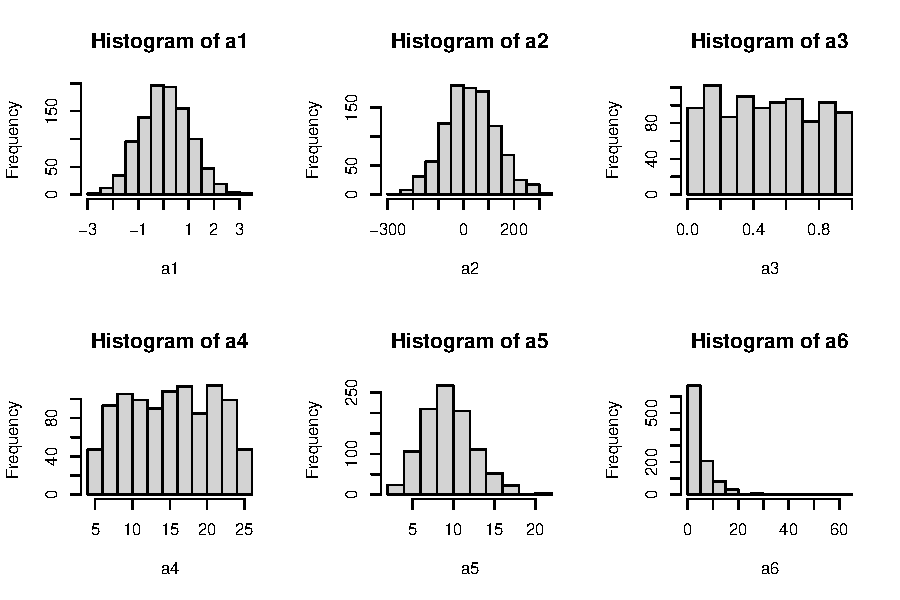
\includegraphics[keepaspectratio]{chapters/ch05_files/figure-pdf/unnamed-chunk-21-1.pdf}}

\begin{Shaded}
\begin{Highlighting}[]
\CommentTok{\# reset graphical parameters}
\CommentTok{\# so the next figure is 1 x 1 panel}
\FunctionTok{par}\NormalTok{(}\AttributeTok{mfrow=}\FunctionTok{c}\NormalTok{(}\DecValTok{1}\NormalTok{,}\DecValTok{1}\NormalTok{))}
\end{Highlighting}
\end{Shaded}

\section{Selecting data with square brackets}\label{sec-manip-select}

One of the most common data manipulation tasks is selecting, or
\textbf{extracting}, from your data. The most common way of selecting
subsets of an object (aka: extracting) is the R \textbf{bracket
notation}. This refers to the symbols used, \texttt{{[}{]}}. These are
also sometimes called \textbf{square brackets}, to distinguish them from
\textbf{curly brackets}, \texttt{\{\}}. The latter are more properly
called \textbf{braces} and have a different purpose in R.

Brackets tell R that you want a part of an object. Which part is
determined either by a name, or an \textbf{index} inside the brackets.
Indices should usually be supplied as numbers, but other types can be
used. For objects with more than 1 dimension, you need to supply as many
indices, or vectors of indices, as the object has dimensions. Within
brackets, vectors of indices are separated by commas.

Brackets can also be used to exclude certain elements by using the
negative sign, but this can be tricky. We'll explore how negative
indices work below.

\subsection{Basics of brackets}\label{sec-manip-select-bas}

The most direct way to work with most R objects is the \textbf{bracket
notation}. Square brackets \texttt{{[}{]}} allow you to access parts of
objects with a simple syntax to specify position within the object.

\begin{figure}[H]

\caption{Illustration of how bracket notation accesses elements of
vector-like objects in R.}

{\centering \pandocbounded{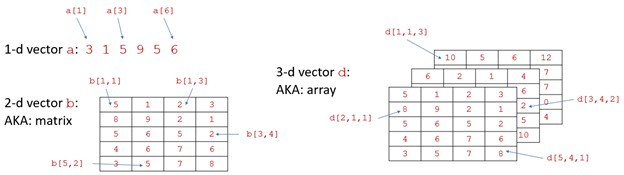
\includegraphics[keepaspectratio]{chapters/../images/05_01.jpg}}

}

\end{figure}%

Positions within an object are accessed using bracket notation. For
example, \texttt{a{[}3{]}} denotes the third element of vector a. For
vectors with \(>1\) dimension, commas are used to separate dimensions.
The first dimension is rows, the second dimension is columns, and the
third dimension is layers (maybe?). The general term for the dimensions
of an object rows, columns, etc., is \textbf{margins}. So, the rows are
the first margin, the columns are the second margin, and so on.

The values inside the brackets that specify rows or columns or whatever
are called \textbf{indices}. In R, \emph{indices start at 1} (this is
unlike some other languages, like Python). The trickiest part of bracket
notation is that you must specify indices for each margin. If you don't,
you will either get an error (bad) or something unexpected (worse).
Indices can be a single value, a vector of values, or left blank to
request all values.

\begin{figure}[H]

\caption{In R bracket notation, the comma separates margins and allows
you to select an entire margin worth of values.}

{\centering \pandocbounded{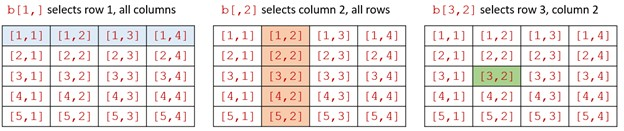
\includegraphics[keepaspectratio]{chapters/../images/05_02.jpg}}

}

\end{figure}%

\subsubsection{Selecting from a vector}\label{sec-manip-select-bas-vec}

Vectors have 1 dimension, so you must specify a single vector of
indices. Notice that the brackets can be empty, in which case all
elements can be returned. If the vector supplied is of length 0, then no
elements will be returned. When a vector of indices with \(>0\) elements
is specified, R will return the elements of the vector in the order
requested. For example, \texttt{a{[}c(1,3,5){]}} and
\texttt{a{[}c(3,5,1){]}} will return the same values but in different
order.

\begin{Shaded}
\begin{Highlighting}[]
\NormalTok{a }\OtherTok{\textless{}{-}} \DecValTok{11}\SpecialCharTok{:}\DecValTok{20}
\CommentTok{\# all elements returned}
\NormalTok{a[]        }
\DocumentationTok{\#\#  [1] 11 12 13 14 15 16 17 18 19 20}

\CommentTok{\# second element}
\NormalTok{a[}\DecValTok{2}\NormalTok{]}
\DocumentationTok{\#\# [1] 12}

\CommentTok{\# elements 3, 4, 5, 6, and 7}
\NormalTok{a[}\DecValTok{3}\SpecialCharTok{:}\DecValTok{7}\NormalTok{]}
\DocumentationTok{\#\# [1] 13 14 15 16 17}

\CommentTok{\# error (not run)}
\CommentTok{\# a[3:7,2]    }

\CommentTok{\# correct version of previous command}
\NormalTok{a[}\FunctionTok{c}\NormalTok{(}\DecValTok{3}\SpecialCharTok{:}\DecValTok{7}\NormalTok{,}\DecValTok{2}\NormalTok{)]}
\DocumentationTok{\#\# [1] 13 14 15 16 17 12}

\CommentTok{\# notice different ordering from previous command}
\NormalTok{a[}\FunctionTok{c}\NormalTok{(}\DecValTok{2}\SpecialCharTok{:}\DecValTok{7}\NormalTok{)]   }
\DocumentationTok{\#\# [1] 12 13 14 15 16 17}
\end{Highlighting}
\end{Shaded}

\subsubsection{Selecting from a matrix}\label{sec-manip-select-bas-mat}

Matrices have 2 dimensions, so you must specify two dimension's worth of
indices. If you want all of one dimension (e.g., rows 1 to 3 and all
columns), you can leave the spot for the index blank. Separate the
dimensions using a comma. Positive indices select elements; negative
elements remove elements.

I'll reiterate this because it is a common mistake: you must specify all
dimensions using a comma. Failing to do so will result in an error (bad)
or unexpected results (worse).

\textbf{Remember: in R, indices start at 1. In some languages such as
Python indices start at 0. R is not Python.}

\begin{Shaded}
\begin{Highlighting}[]

\NormalTok{a }\OtherTok{\textless{}{-}} \FunctionTok{matrix}\NormalTok{(}\DecValTok{1}\SpecialCharTok{:}\DecValTok{12}\NormalTok{, }\AttributeTok{nrow=}\DecValTok{3}\NormalTok{, }\AttributeTok{byrow=}\ConstantTok{TRUE}\NormalTok{)}
\NormalTok{a}
\DocumentationTok{\#\#      [,1] [,2] [,3] [,4]}
\DocumentationTok{\#\# [1,]    1    2    3    4}
\DocumentationTok{\#\# [2,]    5    6    7    8}
\DocumentationTok{\#\# [3,]    9   10   11   12}

\CommentTok{\# value in row 1, column 2}
\NormalTok{a[}\DecValTok{1}\NormalTok{,}\DecValTok{2}\NormalTok{]}
\DocumentationTok{\#\# [1] 2}

\CommentTok{\# values in rows 1{-}3 and columns 1{-}2}
\NormalTok{a[}\DecValTok{1}\SpecialCharTok{:}\DecValTok{3}\NormalTok{, }\DecValTok{1}\SpecialCharTok{:}\DecValTok{2}\NormalTok{]}
\DocumentationTok{\#\#      [,1] [,2]}
\DocumentationTok{\#\# [1,]    1    2}
\DocumentationTok{\#\# [2,]    5    6}
\DocumentationTok{\#\# [3,]    9   10}

\CommentTok{\# rows 1 and 2, all columns}
\NormalTok{a[}\DecValTok{1}\SpecialCharTok{:}\DecValTok{2}\NormalTok{,]}
\DocumentationTok{\#\#      [,1] [,2] [,3] [,4]}
\DocumentationTok{\#\# [1,]    1    2    3    4}
\DocumentationTok{\#\# [2,]    5    6    7    8}

\CommentTok{\# columns 1 and 2, all rows}
\NormalTok{a[,}\DecValTok{1}\SpecialCharTok{:}\DecValTok{2}\NormalTok{]}
\DocumentationTok{\#\#      [,1] [,2]}
\DocumentationTok{\#\# [1,]    1    2}
\DocumentationTok{\#\# [2,]    5    6}
\DocumentationTok{\#\# [3,]    9   10}
\end{Highlighting}
\end{Shaded}

Negative indices remove elements, or return all positive indices.

\begin{Shaded}
\begin{Highlighting}[]
\CommentTok{\# rows except for row 1}
\NormalTok{a[}\SpecialCharTok{{-}}\DecValTok{1}\NormalTok{,]}
\end{Highlighting}
\end{Shaded}

\begin{verbatim}
     [,1] [,2] [,3] [,4]
[1,]    5    6    7    8
[2,]    9   10   11   12
\end{verbatim}

Removing multiple elements with \texttt{-} can be a bit tricky. All
elements of the vector of things to remove must be negative. In the
first example below, R returns an error because you request elements -1,
0, 1, and 2. Element -1 does not exist, and you don't want elements 1
and 2!

\begin{Shaded}
\begin{Highlighting}[]
\CommentTok{\# try to request rows except for}
\CommentTok{\# rows 1 and 2}
\CommentTok{\# not run (error):}
\NormalTok{a[}\SpecialCharTok{{-}}\DecValTok{1}\SpecialCharTok{:}\DecValTok{2}\NormalTok{,]}
\end{Highlighting}
\end{Shaded}

There are several correct ways to get rows other than 1 and 2. Notice
that all of them result in indices with a 1-, a -2, and no positive
values. The first option is probably the best for most situations.

\begin{Shaded}
\begin{Highlighting}[]
\NormalTok{a[}\SpecialCharTok{{-}}\FunctionTok{c}\NormalTok{(}\DecValTok{1}\NormalTok{,}\DecValTok{2}\NormalTok{),]}
\DocumentationTok{\#\# [1]  9 10 11 12}
\NormalTok{a[}\SpecialCharTok{{-}}\DecValTok{1}\SpecialCharTok{*}\DecValTok{1}\SpecialCharTok{:}\DecValTok{2}\NormalTok{,]}
\DocumentationTok{\#\# [1]  9 10 11 12}
\NormalTok{a[}\SpecialCharTok{{-}}\DecValTok{2}\SpecialCharTok{:}\DecValTok{0}\NormalTok{,] }\CommentTok{\# includes {-}2, {-}1, and 0,}
\DocumentationTok{\#\# [1]  9 10 11 12}
         \CommentTok{\# but 0 doesn\textquotesingle{}t do anything}
\end{Highlighting}
\end{Shaded}

Notice that all three of the commands above return a vector, not a
matrix. This is because a single row or column of a matrix simplifies to
a vector. If you want to keep your result in matrix format, you can
specify this using the argument \texttt{drop=FALSE} after the last
dimension and a comma:

\begin{Shaded}
\begin{Highlighting}[]
\NormalTok{a[}\SpecialCharTok{{-}}\FunctionTok{c}\NormalTok{(}\DecValTok{1}\NormalTok{,}\DecValTok{2}\NormalTok{),,drop}\OtherTok{=}\ConstantTok{FALSE}\NormalTok{]}
\end{Highlighting}
\end{Shaded}

\begin{verbatim}
     [,1] [,2] [,3] [,4]
[1,]    9   10   11   12
\end{verbatim}

\subsubsection{Selecting from an array}\label{sec-manip-select-bas-arr}

Selecting from an array is a lot like selecting from a matrix, only with
one more dimension. Consider an array with 3 dimensions: rows, columns,
and ``layers''\footnote{I don't know if there is an actual name for
  this, but I like to call them layers.}.

\begin{Shaded}
\begin{Highlighting}[]
\NormalTok{Ar }\OtherTok{\textless{}{-}} \FunctionTok{array}\NormalTok{(}\DecValTok{1}\SpecialCharTok{:}\DecValTok{24}\NormalTok{, }\AttributeTok{dim=}\FunctionTok{c}\NormalTok{(}\DecValTok{4}\NormalTok{,}\DecValTok{2}\NormalTok{,}\DecValTok{3}\NormalTok{))}
\NormalTok{Ar}
\end{Highlighting}
\end{Shaded}

\begin{verbatim}
, , 1

     [,1] [,2]
[1,]    1    5
[2,]    2    6
[3,]    3    7
[4,]    4    8

, , 2

     [,1] [,2]
[1,]    9   13
[2,]   10   14
[3,]   11   15
[4,]   12   16

, , 3

     [,1] [,2]
[1,]   17   21
[2,]   18   22
[3,]   19   23
[4,]   20   24
\end{verbatim}

Each element in any dimension of the array is a 2-dimensional slice of
the array--i.e., a matrix:

\begin{Shaded}
\begin{Highlighting}[]
\NormalTok{Ar[}\DecValTok{1}\NormalTok{,,]}
\DocumentationTok{\#\#      [,1] [,2] [,3]}
\DocumentationTok{\#\# [1,]    1    9   17}
\DocumentationTok{\#\# [2,]    5   13   21}
\NormalTok{Ar[,}\DecValTok{2}\NormalTok{,]}
\DocumentationTok{\#\#      [,1] [,2] [,3]}
\DocumentationTok{\#\# [1,]    5   13   21}
\DocumentationTok{\#\# [2,]    6   14   22}
\DocumentationTok{\#\# [3,]    7   15   23}
\DocumentationTok{\#\# [4,]    8   16   24}
\NormalTok{Ar[,,}\DecValTok{3}\NormalTok{]}
\DocumentationTok{\#\#      [,1] [,2]}
\DocumentationTok{\#\# [1,]   17   21}
\DocumentationTok{\#\# [2,]   18   22}
\DocumentationTok{\#\# [3,]   19   23}
\DocumentationTok{\#\# [4,]   20   24}
\end{Highlighting}
\end{Shaded}

The images below show what happened. For \texttt{Ar{[}1,,{]}}, the
values in the first row (dimension 1), all columns (dimension 2), and
all layers (dimension 3) were selected. Dimension 2 in the input
\texttt{Ar} became dimension 1 in the output, and dimension 3 in
\texttt{Ar} became dimension 2 in the output.

\begin{figure}[H]

\caption{R bracket notation carries across dimensions within an array,
but the result may not be what you expect. Notice how rows are converted
to columns.}

{\centering \pandocbounded{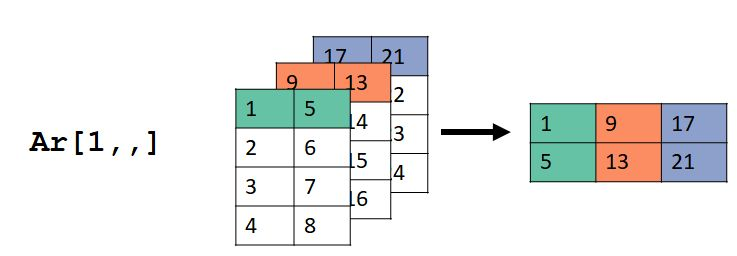
\includegraphics[keepaspectratio]{chapters/../images/05_03.jpg}}

}

\end{figure}%

For \texttt{Ar{[},2,{]}}, the values in the second column (dimension 2),
all rows (dimension 1), and all layers (dimension 3) were selected.
Dimension 2 in the input \texttt{Ar} became dimension 1 in the output,
and dimension 3 in \texttt{Ar} became dimension 2 in the output.

\begin{figure}[H]

\caption{Another example of R bracket notation behavior across layers of
an array.}

{\centering \pandocbounded{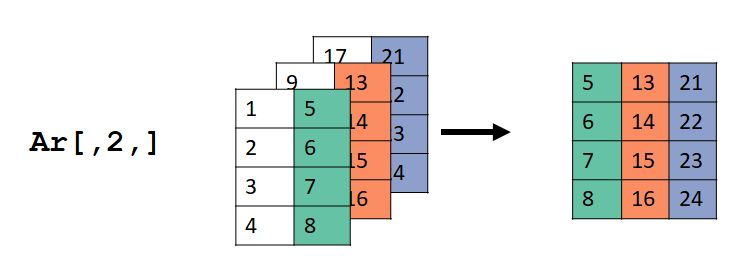
\includegraphics[keepaspectratio]{chapters/../images/05_04.jpg}}

}

\end{figure}%

For \texttt{Ar{[},,3{]}}, the values in the all rows (dimension 1), all
columns (dimension 2), and layer 3 (dimension 3) were selected.
Dimension 2 in the input \texttt{Ar} became dimension 1 in the output,
and dimension 3 in \texttt{Ar} became dimension 2 in the output.

\begin{figure}[H]

\caption{Selecting an entire ``layer'' of a 3-dimensional array.}

{\centering \pandocbounded{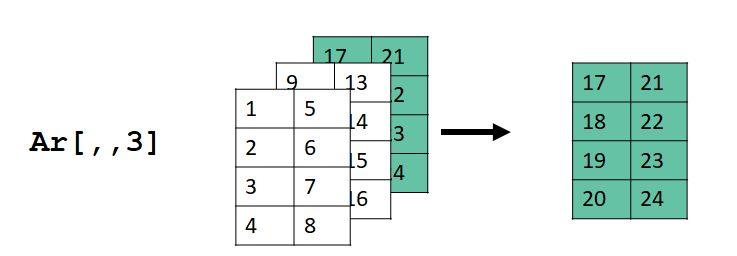
\includegraphics[keepaspectratio]{chapters/../images/05_05.jpg}}

}

\end{figure}%

Selecting by \(\ge\) 1 dimension can be tricky. Consider this example:

\begin{Shaded}
\begin{Highlighting}[]
\NormalTok{Ar[}\DecValTok{1}\NormalTok{,,}\DecValTok{1}\SpecialCharTok{:}\DecValTok{2}\NormalTok{]}
\DocumentationTok{\#\#      [,1] [,2]}
\DocumentationTok{\#\# [1,]    1    9}
\DocumentationTok{\#\# [2,]    5   13}
\end{Highlighting}
\end{Shaded}

Here we selected the first row (dimension 1), all columns (dimension 2),
and layers 1 and 2 (dimension 3).

\begin{figure}[H]

\caption{Illustration of selecting the first 2 rows of teh first 2
elements of a 4 by 2 by 3 array.}

{\centering \pandocbounded{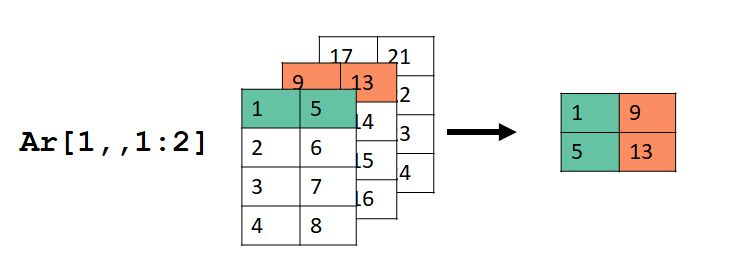
\includegraphics[keepaspectratio]{chapters/../images/05_06.jpg}}

}

\end{figure}%

And if you want a headache, consider this example:

\begin{Shaded}
\begin{Highlighting}[]
\NormalTok{Ar[}\DecValTok{1}\SpecialCharTok{:}\DecValTok{2}\NormalTok{,,}\DecValTok{2}\SpecialCharTok{:}\DecValTok{1}\NormalTok{]}
\DocumentationTok{\#\# , , 1}
\DocumentationTok{\#\# }
\DocumentationTok{\#\#      [,1] [,2]}
\DocumentationTok{\#\# [1,]    9   13}
\DocumentationTok{\#\# [2,]   10   14}
\DocumentationTok{\#\# }
\DocumentationTok{\#\# , , 2}
\DocumentationTok{\#\# }
\DocumentationTok{\#\#      [,1] [,2]}
\DocumentationTok{\#\# [1,]    1    5}
\DocumentationTok{\#\# [2,]    2    6}
\end{Highlighting}
\end{Shaded}

\begin{figure}[H]

\caption{Sometimes, R bracket notation defies common sense.}

{\centering \pandocbounded{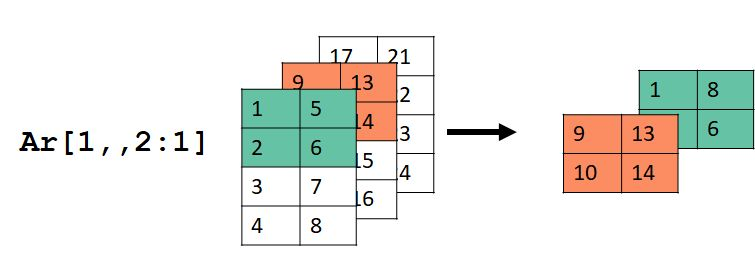
\includegraphics[keepaspectratio]{chapters/../images/05_07.jpg}}

}

\end{figure}%

I can't think of a reason why you would need to do something like the
last example, but it's nice to know that you could.

\subsubsection{Selecting from a data
frame}\label{sec-manip-select-bas-df}

Selecting from a data frame using brackets is largely the same as
selecting from a matrix. Just keep in mind that the result might come
back as a vector (if you select rows in a single column) or a data frame
(any other situation).

\begin{figure}[H]

\caption{Illustration of how bracket notation works on data frames,
which are not matrices despite their appearance.}

{\centering \pandocbounded{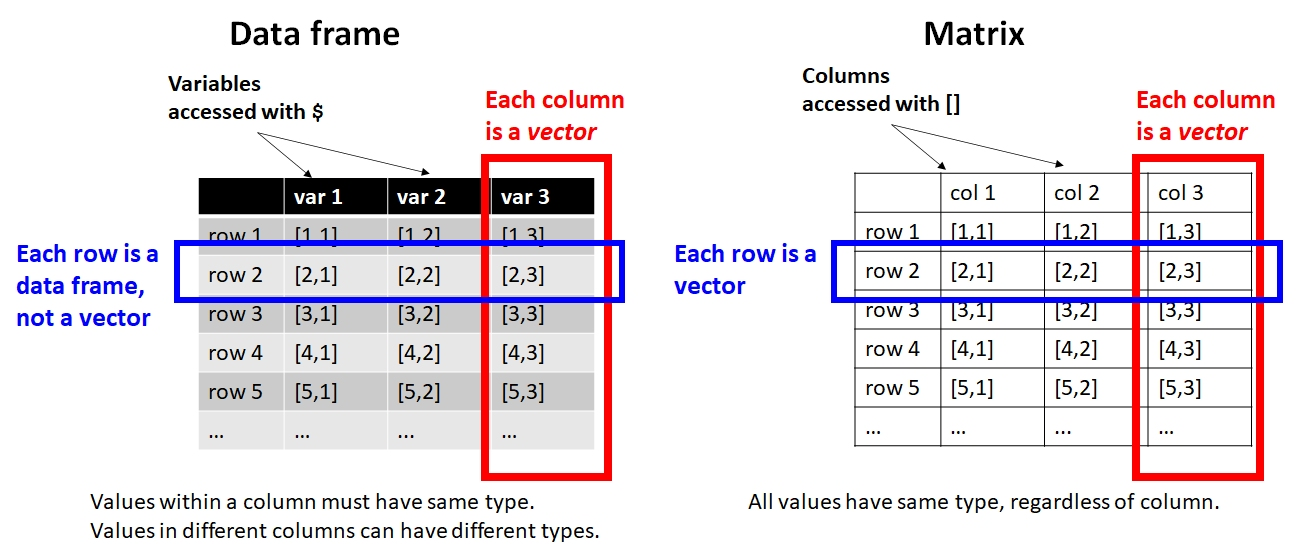
\includegraphics[keepaspectratio]{chapters/../images/05_08.jpg}}

}

\end{figure}%

\begin{Shaded}
\begin{Highlighting}[]
\CommentTok{\# make a small data frame from}
\CommentTok{\# the first 5 rows of iris}
\NormalTok{a }\OtherTok{\textless{}{-}}\NormalTok{ iris[}\DecValTok{1}\SpecialCharTok{:}\DecValTok{5}\NormalTok{,]}

\CommentTok{\# returns a vector}
\NormalTok{a[,}\DecValTok{1}\NormalTok{]}
\DocumentationTok{\#\# [1] 5.1 4.9 4.7 4.6 5.0}

\CommentTok{\# returns a data frame}
\NormalTok{a[}\DecValTok{1}\NormalTok{,]}
\DocumentationTok{\#\#   Sepal.Length Sepal.Width Petal.Length Petal.Width Species}
\DocumentationTok{\#\# 1          5.1         3.5          1.4         0.2  setosa}

\CommentTok{\# returns a data frame}
\NormalTok{a[}\DecValTok{1}\SpecialCharTok{:}\DecValTok{3}\NormalTok{,]}
\DocumentationTok{\#\#   Sepal.Length Sepal.Width Petal.Length Petal.Width Species}
\DocumentationTok{\#\# 1          5.1         3.5          1.4         0.2  setosa}
\DocumentationTok{\#\# 2          4.9         3.0          1.4         0.2  setosa}
\DocumentationTok{\#\# 3          4.7         3.2          1.3         0.2  setosa}

\CommentTok{\# returns a data frame}
\NormalTok{a[}\DecValTok{1}\SpecialCharTok{:}\DecValTok{3}\NormalTok{, }\DecValTok{1}\SpecialCharTok{:}\DecValTok{3}\NormalTok{]}
\DocumentationTok{\#\#   Sepal.Length Sepal.Width Petal.Length}
\DocumentationTok{\#\# 1          5.1         3.5          1.4}
\DocumentationTok{\#\# 2          4.9         3.0          1.4}
\DocumentationTok{\#\# 3          4.7         3.2          1.3}
\end{Highlighting}
\end{Shaded}

\subsubsection{Selecting from lists}\label{sec-manip-select-bas-list}

One of the most important kinds of R object is the \textbf{list}. A list
can be thought of like a series of containers or buckets. Each bucket
can contain completely unrelated things, or even other series of
buckets. Each bucket is called an \textbf{element} of the list. Because
of this flexibility, lists are extremely versatile and useful in R
programming. Many function outputs are really lists (e.g., the outputs
of \texttt{lm()} or \texttt{t.test()}).

Single elements of a list can be accessed with \textbf{double brackets}
\texttt{{[}{[}{]}{]}}. Elements can be selected by name or by index.
Elements that have a name can be selected by name using the \texttt{\$}
symbol instead of by double brackets.

\begin{Shaded}
\begin{Highlighting}[]
\CommentTok{\# make a list "a"}
\NormalTok{x }\OtherTok{\textless{}{-}} \FunctionTok{runif}\NormalTok{(}\DecValTok{10}\NormalTok{)}
\NormalTok{y }\OtherTok{\textless{}{-}} \StringTok{"zebra"}
\NormalTok{z }\OtherTok{\textless{}{-}} \FunctionTok{matrix}\NormalTok{(}\DecValTok{1}\SpecialCharTok{:}\DecValTok{12}\NormalTok{, }\AttributeTok{nrow=}\DecValTok{3}\NormalTok{)}
\NormalTok{a }\OtherTok{\textless{}{-}} \FunctionTok{list}\NormalTok{(}\AttributeTok{e1=}\NormalTok{x, }\AttributeTok{e2=}\NormalTok{y, }\AttributeTok{e3=}\NormalTok{z)}

\NormalTok{a[[}\DecValTok{1}\NormalTok{]]}
\DocumentationTok{\#\#  [1] 0.81537826 0.85151339 0.94974433 0.24860408 0.20883937 0.23072284}
\DocumentationTok{\#\#  [7] 0.80287954 0.06142657 0.65110133 0.21388695}
\NormalTok{a[[}\DecValTok{2}\NormalTok{]]}
\DocumentationTok{\#\# [1] "zebra"}
\NormalTok{a[[}\StringTok{"e1"}\NormalTok{]]}
\DocumentationTok{\#\#  [1] 0.81537826 0.85151339 0.94974433 0.24860408 0.20883937 0.23072284}
\DocumentationTok{\#\#  [7] 0.80287954 0.06142657 0.65110133 0.21388695}
\NormalTok{a}\SpecialCharTok{$}\NormalTok{e1}
\DocumentationTok{\#\#  [1] 0.81537826 0.85151339 0.94974433 0.24860408 0.20883937 0.23072284}
\DocumentationTok{\#\#  [7] 0.80287954 0.06142657 0.65110133 0.21388695}
\end{Highlighting}
\end{Shaded}

Multiple elements of a list can be selected using \textbf{single
brackets}. Doing so will return a new list containing the requested
elements, \textbf{not} the requested elements themselves. This can be a
little confusing. Compare the following two commands and notice that the
first returns the 10 random numbers in the first element of \texttt{a},
while the second returns a list with 1 element, and that element is the
numbers 1 through 10.

\begin{Shaded}
\begin{Highlighting}[]
\NormalTok{a[[}\DecValTok{1}\NormalTok{]]}
\DocumentationTok{\#\#  [1] 0.81537826 0.85151339 0.94974433 0.24860408 0.20883937 0.23072284}
\DocumentationTok{\#\#  [7] 0.80287954 0.06142657 0.65110133 0.21388695}
\NormalTok{a[}\DecValTok{1}\NormalTok{]}
\DocumentationTok{\#\# $e1}
\DocumentationTok{\#\#  [1] 0.81537826 0.85151339 0.94974433 0.24860408 0.20883937 0.23072284}
\DocumentationTok{\#\#  [7] 0.80287954 0.06142657 0.65110133 0.21388695}
\end{Highlighting}
\end{Shaded}

Next, observe what happens when we select more than one element of the
list \texttt{a}. The output is a list.

\begin{Shaded}
\begin{Highlighting}[]
\NormalTok{a[}\DecValTok{1}\SpecialCharTok{:}\DecValTok{2}\NormalTok{]}
\DocumentationTok{\#\# $e1}
\DocumentationTok{\#\#  [1] 0.81537826 0.85151339 0.94974433 0.24860408 0.20883937 0.23072284}
\DocumentationTok{\#\#  [7] 0.80287954 0.06142657 0.65110133 0.21388695}
\DocumentationTok{\#\# }
\DocumentationTok{\#\# $e2}
\DocumentationTok{\#\# [1] "zebra"}
\FunctionTok{class}\NormalTok{(a[}\DecValTok{1}\SpecialCharTok{:}\DecValTok{2}\NormalTok{])}
\DocumentationTok{\#\# [1] "list"}
\end{Highlighting}
\end{Shaded}

The reason for this syntax is that the single brackets notation allows
you to extract multiple elements of the list at once to quickly make a
new list.

\begin{Shaded}
\begin{Highlighting}[]
\NormalTok{a2 }\OtherTok{\textless{}{-}}\NormalTok{ a[}\DecValTok{1}\SpecialCharTok{:}\DecValTok{2}\NormalTok{]}
\NormalTok{a2}
\end{Highlighting}
\end{Shaded}

\begin{verbatim}
$e1
 [1] 0.81537826 0.85151339 0.94974433 0.24860408 0.20883937 0.23072284
 [7] 0.80287954 0.06142657 0.65110133 0.21388695

$e2
[1] "zebra"
\end{verbatim}

\subsection{Selecting and extracting with logical
tests}\label{selecting-and-extracting-with-logical-tests}

Selecting data from a data frame is one of the most common data
manipulations. R offers several ways to accomplish this. One of the most
fundamental is the function \texttt{which()}, returns the indices in a
vector where a logical condition is \texttt{TRUE}. This means that you
can select any piece of a dataset that can be identified logically.
Consider the example below, which extracts the rows of the \texttt{iris}
dataset where the variable \texttt{Species} matches the character string
\texttt{"setosa"}.

\begin{Shaded}
\begin{Highlighting}[]
\CommentTok{\# not run (long output); try it on your machine!}
\NormalTok{iris[}\FunctionTok{which}\NormalTok{(iris}\SpecialCharTok{$}\NormalTok{Species }\SpecialCharTok{==} \StringTok{"setosa"}\NormalTok{),]}

\CommentTok{\# better: define which indices you want,}
\CommentTok{\#         and make selection in separate}
\CommentTok{\#         commands.}
\NormalTok{flag }\OtherTok{\textless{}{-}} \FunctionTok{which}\NormalTok{(iris}\SpecialCharTok{$}\NormalTok{Species }\SpecialCharTok{==} \StringTok{"setosa"}\NormalTok{)}
\NormalTok{iris[flag,]}
\end{Highlighting}
\end{Shaded}

In most situations, \texttt{which()} can be omitted because it is
implicit in the command. However, not using it can sometimes produce
strange results. Because of this, I always use \texttt{which()} in my
code. Including \texttt{which()} can also make your code a little
clearer to someone who is not familiar with R. For example, the two
commands below are exactly equivalent:

\begin{Shaded}
\begin{Highlighting}[]
\CommentTok{\# not run (long output); try it on your machine!}
\NormalTok{iris[}\FunctionTok{which}\NormalTok{(iris}\SpecialCharTok{$}\NormalTok{Species }\SpecialCharTok{==} \StringTok{"setosa"}\NormalTok{),]}
\NormalTok{iris[iris}\SpecialCharTok{$}\NormalTok{Species }\SpecialCharTok{==} \StringTok{"setosa"}\NormalTok{,]}
\end{Highlighting}
\end{Shaded}

What \texttt{which()} is really doing in the commands above is returning
a vector of numbers. That vector is then used by the containing brackets
\texttt{{[}{]}} to determine which pieces of the data frame to pull. The
numbers returned by \texttt{which()} are the indices at which a logical
vector is TRUE. Compare the results of the two commands below, which
were used in the commands above to select from \texttt{iris}:

\begin{Shaded}
\begin{Highlighting}[]

\CommentTok{\# logical vector:}
\NormalTok{iris}\SpecialCharTok{$}\NormalTok{Species }\SpecialCharTok{==} \StringTok{"setosa"}
\DocumentationTok{\#\#   [1]  TRUE  TRUE  TRUE  TRUE  TRUE  TRUE  TRUE  TRUE  TRUE  TRUE  TRUE  TRUE}
\DocumentationTok{\#\#  [13]  TRUE  TRUE  TRUE  TRUE  TRUE  TRUE  TRUE  TRUE  TRUE  TRUE  TRUE  TRUE}
\DocumentationTok{\#\#  [25]  TRUE  TRUE  TRUE  TRUE  TRUE  TRUE  TRUE  TRUE  TRUE  TRUE  TRUE  TRUE}
\DocumentationTok{\#\#  [37]  TRUE  TRUE  TRUE  TRUE  TRUE  TRUE  TRUE  TRUE  TRUE  TRUE  TRUE  TRUE}
\DocumentationTok{\#\#  [49]  TRUE  TRUE FALSE FALSE FALSE FALSE FALSE FALSE FALSE FALSE FALSE FALSE}
\DocumentationTok{\#\#  [61] FALSE FALSE FALSE FALSE FALSE FALSE FALSE FALSE FALSE FALSE FALSE FALSE}
\DocumentationTok{\#\#  [73] FALSE FALSE FALSE FALSE FALSE FALSE FALSE FALSE FALSE FALSE FALSE FALSE}
\DocumentationTok{\#\#  [85] FALSE FALSE FALSE FALSE FALSE FALSE FALSE FALSE FALSE FALSE FALSE FALSE}
\DocumentationTok{\#\#  [97] FALSE FALSE FALSE FALSE FALSE FALSE FALSE FALSE FALSE FALSE FALSE FALSE}
\DocumentationTok{\#\# [109] FALSE FALSE FALSE FALSE FALSE FALSE FALSE FALSE FALSE FALSE FALSE FALSE}
\DocumentationTok{\#\# [121] FALSE FALSE FALSE FALSE FALSE FALSE FALSE FALSE FALSE FALSE FALSE FALSE}
\DocumentationTok{\#\# [133] FALSE FALSE FALSE FALSE FALSE FALSE FALSE FALSE FALSE FALSE FALSE FALSE}
\DocumentationTok{\#\# [145] FALSE FALSE FALSE FALSE FALSE FALSE}

\CommentTok{\# which identifies which elements of vector are TRUE:}
\FunctionTok{which}\NormalTok{(iris}\SpecialCharTok{$}\NormalTok{Species }\SpecialCharTok{==} \StringTok{"setosa"}\NormalTok{)}
\DocumentationTok{\#\#  [1]  1  2  3  4  5  6  7  8  9 10 11 12 13 14 15 16 17 18 19 20 21 22 23 24 25}
\DocumentationTok{\#\# [26] 26 27 28 29 30 31 32 33 34 35 36 37 38 39 40 41 42 43 44 45 46 47 48 49 50}
\end{Highlighting}
\end{Shaded}

Multiple conditions can be used to select data using the \texttt{\&}
(and) and \texttt{\textbar{}} (or) operators.

\begin{Shaded}
\begin{Highlighting}[]
\CommentTok{\# not run (long output):}
\NormalTok{iris[}\FunctionTok{which}\NormalTok{(iris}\SpecialCharTok{$}\NormalTok{Species }\SpecialCharTok{==} \StringTok{"versicolor"} \SpecialCharTok{\&}\NormalTok{ iris}\SpecialCharTok{$}\NormalTok{Petal.Length }\SpecialCharTok{\textless{}=} \DecValTok{4}\NormalTok{),]}

\NormalTok{iris[}\FunctionTok{which}\NormalTok{(iris}\SpecialCharTok{$}\NormalTok{Species }\SpecialCharTok{==} \StringTok{"versicolor"} \SpecialCharTok{|}\NormalTok{ iris}\SpecialCharTok{$}\NormalTok{Petal.Length }\SpecialCharTok{\textless{}=} \FloatTok{1.6}\NormalTok{),]}
\end{Highlighting}
\end{Shaded}

The examples above could also be accomplished in several lines; in fact,
splitting the selection criteria up can make for cleaner code. The
commands below also show how splitting the selection commands up can
help you abide by the ``single point of definition'' principle.

\begin{Shaded}
\begin{Highlighting}[]
\CommentTok{\# not run (long output):}
\NormalTok{flag1 }\OtherTok{\textless{}{-}}\NormalTok{ iris}\SpecialCharTok{$}\NormalTok{Species }\SpecialCharTok{==} \StringTok{"versicolor"}
\NormalTok{flag2 }\OtherTok{\textless{}{-}}\NormalTok{ iris}\SpecialCharTok{$}\NormalTok{Petal.Length }\SpecialCharTok{\textless{}=} \DecValTok{4}

\DocumentationTok{\#\# meet both conditions:}
\NormalTok{iris[flag1 }\SpecialCharTok{\&}\NormalTok{ flag2,]}
\NormalTok{iris[}\FunctionTok{intersect}\NormalTok{(flag1, flag2),]}

\DocumentationTok{\#\# meet either condition}
\NormalTok{iris[flag1 }\SpecialCharTok{|}\NormalTok{ flag2,]}
\NormalTok{iris[}\FunctionTok{union}\NormalTok{(flag1, flag2),]}
\end{Highlighting}
\end{Shaded}

More than 2 conditions can be combined just as easily:

\begin{Shaded}
\begin{Highlighting}[]
\NormalTok{flag1 }\OtherTok{\textless{}{-}}\NormalTok{ iris}\SpecialCharTok{$}\NormalTok{Species }\SpecialCharTok{==} \StringTok{"versicolor"}
\NormalTok{flag2 }\OtherTok{\textless{}{-}}\NormalTok{ iris}\SpecialCharTok{$}\NormalTok{Petal.Length }\SpecialCharTok{\textless{}=} \DecValTok{4}
\NormalTok{flag3 }\OtherTok{\textless{}{-}}\NormalTok{ iris}\SpecialCharTok{$}\NormalTok{Petal.Length }\SpecialCharTok{\textgreater{}} \FloatTok{0.5}
\NormalTok{iris[flag1 }\SpecialCharTok{\&}\NormalTok{ flag2 }\SpecialCharTok{\&}\NormalTok{ flag3,]}
\end{Highlighting}
\end{Shaded}

\begin{verbatim}
   Sepal.Length Sepal.Width Petal.Length Petal.Width    Species
54          5.5         2.3          4.0         1.3 versicolor
58          4.9         2.4          3.3         1.0 versicolor
60          5.2         2.7          3.9         1.4 versicolor
61          5.0         2.0          3.5         1.0 versicolor
63          6.0         2.2          4.0         1.0 versicolor
65          5.6         2.9          3.6         1.3 versicolor
70          5.6         2.5          3.9         1.1 versicolor
72          6.1         2.8          4.0         1.3 versicolor
80          5.7         2.6          3.5         1.0 versicolor
81          5.5         2.4          3.8         1.1 versicolor
82          5.5         2.4          3.7         1.0 versicolor
83          5.8         2.7          3.9         1.2 versicolor
90          5.5         2.5          4.0         1.3 versicolor
93          5.8         2.6          4.0         1.2 versicolor
94          5.0         2.3          3.3         1.0 versicolor
99          5.1         2.5          3.0         1.1 versicolor
\end{verbatim}

Selections can return 0 matches. This usually manifests as a data frame
or matrix with 0 rows.

\begin{Shaded}
\begin{Highlighting}[]
\NormalTok{flag1 }\OtherTok{\textless{}{-}}\NormalTok{ iris}\SpecialCharTok{$}\NormalTok{Species }\SpecialCharTok{==} \StringTok{"versicolor"}
\NormalTok{flag2 }\OtherTok{\textless{}{-}}\NormalTok{ iris}\SpecialCharTok{$}\NormalTok{Petal.Length }\SpecialCharTok{\textless{}=} \DecValTok{1}
\NormalTok{iris[flag1 }\SpecialCharTok{\&}\NormalTok{ flag2,]}
\end{Highlighting}
\end{Shaded}

\begin{verbatim}
[1] Sepal.Length Sepal.Width  Petal.Length Petal.Width  Species     
<0 rows> (or 0-length row.names)
\end{verbatim}

A related function is the binary operator\footnote{A binary operator
  uses two arguments, one before the symbol and one after. For example,
  \texttt{+} is a binary operator that adds the the argument before the
  \texttt{+} to the argument after the \texttt{+}} \texttt{\%in\%}. For
a command like \texttt{A\ \&in\%\ B}, R returns a vector of logical
values for each element in \texttt{A}, indicating whether those values
occur in \texttt{B}.

\begin{Shaded}
\begin{Highlighting}[]

\NormalTok{A }\OtherTok{\textless{}{-}} \FunctionTok{c}\NormalTok{(}\StringTok{"a"}\NormalTok{, }\StringTok{"b"}\NormalTok{, }\StringTok{"c"}\NormalTok{, }\StringTok{"d"}\NormalTok{, }\StringTok{"e"}\NormalTok{)}
\NormalTok{B }\OtherTok{\textless{}{-}} \FunctionTok{c}\NormalTok{(}\StringTok{"c"}\NormalTok{, }\StringTok{"d"}\NormalTok{, }\StringTok{"e"}\NormalTok{, }\StringTok{"f"}\NormalTok{)}
\NormalTok{A }\SpecialCharTok{\%in\%}\NormalTok{ B}
\DocumentationTok{\#\# [1] FALSE FALSE  TRUE  TRUE  TRUE}
\NormalTok{B }\SpecialCharTok{\%in\%}\NormalTok{ A}
\DocumentationTok{\#\# [1]  TRUE  TRUE  TRUE FALSE}
\end{Highlighting}
\end{Shaded}

While we're here, the set operations \texttt{union()},
\texttt{intersect()}, and \texttt{setdiff()} can be useful for selecting
data.

\begin{Shaded}
\begin{Highlighting}[]
\NormalTok{A }\OtherTok{\textless{}{-}} \FunctionTok{c}\NormalTok{(}\StringTok{"a"}\NormalTok{, }\StringTok{"b"}\NormalTok{, }\StringTok{"c"}\NormalTok{, }\StringTok{"d"}\NormalTok{, }\StringTok{"e"}\NormalTok{)}
\NormalTok{B }\OtherTok{\textless{}{-}} \FunctionTok{c}\NormalTok{(}\StringTok{"c"}\NormalTok{, }\StringTok{"d"}\NormalTok{, }\StringTok{"e"}\NormalTok{, }\StringTok{"f"}\NormalTok{)}

\CommentTok{\# elements in both sets: intersect}
\CommentTok{\# i.e., AND}
\FunctionTok{intersect}\NormalTok{(A, B)}
\DocumentationTok{\#\# [1] "c" "d" "e"}

\CommentTok{\# elements in either set:}
\CommentTok{\# i.e., OR}
\FunctionTok{union}\NormalTok{(A, B)}
\DocumentationTok{\#\# [1] "a" "b" "c" "d" "e" "f"}

\CommentTok{\# elements in first set only:}
\CommentTok{\# (asymmetric)}
\CommentTok{\# i.e., XOR (one{-}sided)}
\FunctionTok{setdiff}\NormalTok{(A, B)}
\DocumentationTok{\#\# [1] "a" "b"}
\FunctionTok{setdiff}\NormalTok{(B, A)}
\DocumentationTok{\#\# [1] "f"}

\CommentTok{\# elements in only one set}
\CommentTok{\# (symmetric)}
\CommentTok{\# i.e., XOR (two{-}sided)}
\FunctionTok{union}\NormalTok{(}\FunctionTok{setdiff}\NormalTok{(A, B), }\FunctionTok{setdiff}\NormalTok{(B, A))}
\DocumentationTok{\#\# [1] "a" "b" "f"}
\end{Highlighting}
\end{Shaded}

One example of how this might be useful is if you want to select
observations from a dataset containing one of several values. The
example below illustrates this with \texttt{iris}:

\begin{Shaded}
\begin{Highlighting}[]
\CommentTok{\# not run (long output):}
\NormalTok{iris[iris}\SpecialCharTok{$}\NormalTok{Species }\SpecialCharTok{\%in\%} \FunctionTok{c}\NormalTok{(}\StringTok{"setosa"}\NormalTok{, }\StringTok{"versicolor"}\NormalTok{),]}
\end{Highlighting}
\end{Shaded}

We'll go over some more complicated selection methods in a future
section, but what you've seen so far can be very powerful.

\section{Dates and temporal data}\label{sec-manip-date}

Most of the data we deal with in R are numbers, but textual and temporal
data are important two. Working with dates, times, and character strings
can be significantly more complicated than working with
numbers\ldots so, I've put together an entire page on it. I am the first
to admit that the approaches demonstrated here are a little
``old-school'' compared to some of the newer packages. In particular,
many people prefer the tidyverse package \texttt{lubridate} (Grolemund
and Wickham 2011) for temporal data. Much of this section is based on
Spector (2008).

Temporal data can be read and interpreted by R in many formats. The
general rule is to use the simplest way that you can, because the date
and time classes can be very complicated. For example, don't store date
and time if you only need date. This doesn't mean to discard potentially
useful data; just to be judicious in what you import to and try to
manipulate in R.

It should be noted that the easiest way to deal with dates and times is
``don't''. In many situations it's actually not necessary to use
temporal data classes. For example, if a field study was conducted in
two years, and there is no temporal component to the question, it might
be sufficient to just call the years \texttt{year1} and \texttt{year2}
in the dataset. Or, if an elapsed time is used as a variable, it might
make more sense to store the elapsed time (e.g., 10 minutes, 11.2
minutes, etc.) rather than use full date/time codes for each observation
time.

\subsection{Dates without times}\label{sec-manip-date-date}

The easiest way to handle dates is to use the base function
\texttt{as.Date()}. This function converts character strings to the R
date format. This implies that you will have a much easier time if you
send dates to R in YYYY-MM-DD format. You can do this in Excel by
setting a custom number format. Once in R, use \texttt{as.Date()} to
convert your properly-formatted text strings into date objects. Once
converted, R can do simple arithmetic such as finding intervals between
dates.

\begin{Shaded}
\begin{Highlighting}[]

\CommentTok{\# enter dates as text strings}
\NormalTok{a }\OtherTok{\textless{}{-}} \FunctionTok{c}\NormalTok{(}\StringTok{"2021{-}07{-}23"}\NormalTok{, }\StringTok{"2021{-}08{-}01"}\NormalTok{, }\StringTok{"2021{-}09{-}03"}\NormalTok{)}

\CommentTok{\# convert to date}
\NormalTok{b }\OtherTok{\textless{}{-}} \FunctionTok{as.Date}\NormalTok{(a)}

\CommentTok{\# check classes}
\FunctionTok{class}\NormalTok{(a)}
\DocumentationTok{\#\# [1] "character"}
\FunctionTok{class}\NormalTok{(b)}
\DocumentationTok{\#\# [1] "Date"}

\CommentTok{\# can do math with dates!}
\NormalTok{b[}\DecValTok{2}\NormalTok{] }\SpecialCharTok{{-}}\NormalTok{ b[}\DecValTok{1}\NormalTok{]}
\DocumentationTok{\#\# Time difference of 9 days}
\end{Highlighting}
\end{Shaded}

The examples above use the
\href{https://en.wikipedia.org/wiki/ISO_8601}{ISO 8601 date format},
Year-Month-Day (or YYYY-MM-DD). This format has the advantage that
sorting it alphanumerically is the same as sorting it chronologically.
Each element has a fixed number of digits to avoid issues like January
and October (months 1 and 10) being sorted next to each other.

I suggest that you get in the habit of storing dates this way. This
format is the default date format in R (and many other programs), such
that R can read dates in this format without additional arguments. If
you insist on storing dates in other formats, you can still read those
dates into R. You just need to tell \texttt{as.Date()} the format that
the date is in. The syntax for formatting dates and times is handled by
the function \texttt{strptime()} (see \texttt{?strptime} for more
examples). Something common to all of the formats below is that each
element has a \emph{fixed number of digits}, 4 for year and 2 for month
or day. This is to avoid ambiguity: does ``7/2/2019'' ``July second,
2019'', or ``February 7, 2019''?. This also avoids issues arising from
treating numbers as character strings. For example, January and October
(months 1 and 10) might be sorted next to each other unless represented
by ``01'' and ``10'' instead of ``1'' and ``10''.

\begin{Shaded}
\begin{Highlighting}[]

\CommentTok{\# YYYYMMDD}
\NormalTok{a }\OtherTok{\textless{}{-}} \StringTok{"20210721"}
\FunctionTok{as.Date}\NormalTok{(a, }\StringTok{"\%Y\%m\%d"}\NormalTok{)}
\DocumentationTok{\#\# [1] "2021{-}07{-}21"}

\CommentTok{\# MMDDYYYY}
\NormalTok{a }\OtherTok{\textless{}{-}} \StringTok{"07212021"}
\FunctionTok{as.Date}\NormalTok{(a, }\StringTok{"\%m\%d\%Y"}\NormalTok{)}
\DocumentationTok{\#\# [1] "2021{-}07{-}21"}

\CommentTok{\# MM/DD/YYYY}
\NormalTok{a }\OtherTok{\textless{}{-}} \StringTok{"07/21/2021"}
\FunctionTok{as.Date}\NormalTok{(a, }\StringTok{"\%m/\%d/\%Y"}\NormalTok{)}
\DocumentationTok{\#\# [1] "2021{-}07{-}21"}

\CommentTok{\# DD{-}MM{-}YYYY}
\NormalTok{a }\OtherTok{\textless{}{-}} \StringTok{"21{-}07{-}2021"}
\FunctionTok{as.Date}\NormalTok{(a, }\StringTok{"\%d{-}\%m{-}\%Y"}\NormalTok{)}
\DocumentationTok{\#\# [1] "2021{-}07{-}21"}
\end{Highlighting}
\end{Shaded}

An even simpler option for dates, if all dates are within the same year,
is to use Julian dates (i.e., day-of-year). If you want to read Julian
dates into R as dates, you can also use \texttt{as.Date()}. Notice in
the example below that the Julian dates must be supplied as
\emph{character strings with 3 digits}, not as numerals. Notice also
that R assigns the current year to the dates unless you specifically
tell it to do something else.

\begin{Shaded}
\begin{Highlighting}[]

\NormalTok{a }\OtherTok{\textless{}{-}} \FunctionTok{as.character}\NormalTok{(}\FunctionTok{c}\NormalTok{(}\DecValTok{204}\NormalTok{, }\DecValTok{213}\NormalTok{, }\DecValTok{246}\NormalTok{))}
\FunctionTok{as.Date}\NormalTok{(a, }\StringTok{"\%j"}\NormalTok{)}
\DocumentationTok{\#\# [1] "2026{-}07{-}23" "2026{-}08{-}01" "2026{-}09{-}03"}

\DocumentationTok{\#\# not run:}
\DocumentationTok{\#\# causes error because nchar("15") \textless{} 3:}
\CommentTok{\#a \textless{}{-} c(15, 204, 213, 246)}
\CommentTok{\#as.Date(a, "\%j")}

\CommentTok{\# convert all numbers to 3 digit}
\CommentTok{\# character strings first with formatC():}
\NormalTok{a }\OtherTok{\textless{}{-}} \FunctionTok{c}\NormalTok{(}\DecValTok{15}\NormalTok{, }\DecValTok{204}\NormalTok{, }\DecValTok{213}\NormalTok{, }\DecValTok{246}\NormalTok{)}
\NormalTok{x }\OtherTok{\textless{}{-}} \FunctionTok{formatC}\NormalTok{(a, }\AttributeTok{width=}\DecValTok{3}\NormalTok{, }\AttributeTok{flag=}\StringTok{"0"}\NormalTok{)}
\FunctionTok{as.Date}\NormalTok{(x, }\StringTok{"\%j"}\NormalTok{)}
\DocumentationTok{\#\# [1] "2026{-}01{-}15" "2026{-}07{-}23" "2026{-}08{-}01" "2026{-}09{-}03"}
\end{Highlighting}
\end{Shaded}

Dates can be reformatted using the function \texttt{format()}. Notice
that the output is a character string, not a date. The syntax for the
conversion comes from \texttt{strptime()}, just as with
\texttt{as.Date()} above. If you need to use a formatted date (character
string) as a date (R class) you need to convert it with
\texttt{as.Date()}.

\begin{Shaded}
\begin{Highlighting}[]

\CommentTok{\# make some dates as character strings and convert to date}
\NormalTok{a }\OtherTok{\textless{}{-}} \FunctionTok{c}\NormalTok{(}\StringTok{"2021{-}07{-}23"}\NormalTok{, }\StringTok{"2021{-}08{-}01"}\NormalTok{, }\StringTok{"2021{-}09{-}03"}\NormalTok{)}
\NormalTok{x }\OtherTok{\textless{}{-}} \FunctionTok{as.Date}\NormalTok{(a)}

\CommentTok{\# Julian day (day of year), as character}
\FunctionTok{format}\NormalTok{(x, }\StringTok{"\%j"}\NormalTok{)}
\DocumentationTok{\#\# [1] "204" "213" "246"}
\CommentTok{\# as number}
\FunctionTok{as.numeric}\NormalTok{(}\FunctionTok{format}\NormalTok{(x, }\StringTok{"\%j"}\NormalTok{))}
\DocumentationTok{\#\# [1] 204 213 246}

\CommentTok{\# ISO format}
\FunctionTok{format}\NormalTok{(x, }\StringTok{"\%Y{-}\%m{-}\%d"}\NormalTok{)}
\DocumentationTok{\#\# [1] "2021{-}07{-}23" "2021{-}08{-}01" "2021{-}09{-}03"}

\CommentTok{\# use month abbreviations, separate by slashes}
\FunctionTok{format}\NormalTok{(x, }\StringTok{"\%b/\%d/\%y"}\NormalTok{)}
\DocumentationTok{\#\# [1] "Jul/23/21" "Aug/01/21" "Sep/03/21"}
\end{Highlighting}
\end{Shaded}

\subsection{Dates with times and time zones}\label{sec-manip-date-time}

\href{https://en.wikipedia.org/wiki/Here_be_dragons}{Here be dragons}.

Things get more complicated when time is included with a date, but the
basic procedures are the same as date-only data. By default, R assumes
that times are in the time zone of the current user. So, if you are
collaborating with someone in a different time zone, you need to account
for time zone in your code. Another default behavior is that R will
assume that times without dates are on the current day.

The main function for working with dates \emph{and} times is
\texttt{strptime()}. This function takes in a character vector and a
format argument, which tells R how the character vector is formatted. It
returns objects of class \texttt{POSIXlt} and \texttt{POSIXt}, which
contain date and time information in a standardized way.

\begin{Shaded}
\begin{Highlighting}[]

\CommentTok{\# create some times as character strings}
\NormalTok{a }\OtherTok{\textless{}{-}} \FunctionTok{c}\NormalTok{(}\StringTok{"01:15:03"}\NormalTok{, }\StringTok{"14:28:21"}\NormalTok{)}

\CommentTok{\# time with seconds}
\FunctionTok{strptime}\NormalTok{(a, }\AttributeTok{format=}\StringTok{"\%H:\%M:\%S"}\NormalTok{)}
\DocumentationTok{\#\# [1] "2026{-}08{-}10 01:15:03 EDT" "2026{-}08{-}10 14:28:21 EDT"}

\CommentTok{\# time with seconds dropped}
\FunctionTok{strptime}\NormalTok{(a, }\AttributeTok{format=}\StringTok{"\%H:\%M"}\NormalTok{)    }\CommentTok{\# seconds dropped}
\DocumentationTok{\#\# [1] "2026{-}08{-}10 01:15:00 EDT" "2026{-}08{-}10 14:28:00 EDT"}
\end{Highlighting}
\end{Shaded}

Notice that the current date was included in the result of
\texttt{strptime()} (at least, the date when I rendered the document).

Time zones should be specified when working with data that contain dates
and times. Remember that R will assume the time is in the current user's
time zone. This almost always means the time zone used by the operating
system in which R is running. If you did something silly like record
data in one time zone and analyze it in another, you have to be careful.
For example, I once ran a field study in Indiana where data were
recorded in Eastern time. But, the office where I analyzed the data was
in Missouri (Central time). R kept converting the time-stamped data to
Central time, which interfered with the analysis until I learned how to
work with time zones in R. To make things worse, data were recorded in
the summer (Eastern daylight time) but analyzed in both early fall
(Central daylight time) and late fall (Central standard time).

\begin{Shaded}
\begin{Highlighting}[]

\CommentTok{\# make some date{-}times and convert to date{-}time class}
\NormalTok{a }\OtherTok{\textless{}{-}} \FunctionTok{c}\NormalTok{(}\StringTok{"2021{-}07{-}23 13:21"}\NormalTok{, }\StringTok{"2021{-}08{-}01 09:15"}\NormalTok{)}
\NormalTok{x }\OtherTok{\textless{}{-}} \FunctionTok{strptime}\NormalTok{(a, }\StringTok{"\%Y{-}\%m{-}\%d \%H:\%M"}\NormalTok{)}
\NormalTok{x}
\DocumentationTok{\#\# [1] "2021{-}07{-}23 13:21:00 EDT" "2021{-}08{-}01 09:15:00 EDT"}

\CommentTok{\# times without dates will be assigned current date:}
\NormalTok{a2 }\OtherTok{\textless{}{-}} \FunctionTok{c}\NormalTok{(}\StringTok{"13:21"}\NormalTok{, }\StringTok{"09:15"}\NormalTok{)}
\NormalTok{x2 }\OtherTok{\textless{}{-}} \FunctionTok{strptime}\NormalTok{(a2, }\StringTok{"\%H:\%M"}\NormalTok{)}
\NormalTok{x2}
\DocumentationTok{\#\# [1] "2026{-}08{-}10 13:21:00 EDT" "2026{-}08{-}10 09:15:00 EDT"}
\end{Highlighting}
\end{Shaded}

Time zone names are not always portable across systems. R has a list of
built-in time zones that it can handle, and these should work, but be
careful and \textbf{\emph{always}} validate any code that depends on
time zones. The list of time zones R can use can be printed to the
console with the command \texttt{OlsonNames()}.

\begin{Shaded}
\begin{Highlighting}[]

\CommentTok{\# US Central Daylight Time (5 hours behind UTC)}
\NormalTok{a }\OtherTok{\textless{}{-}} \FunctionTok{c}\NormalTok{(}\StringTok{"2021{-}07{-}23 13:21"}\NormalTok{, }\StringTok{"2021{-}08{-}01 09:15"}\NormalTok{)}

\CommentTok{\# strptime() will assign whatever time zone you enter:}
\NormalTok{b }\OtherTok{\textless{}{-}} \FunctionTok{strptime}\NormalTok{(a, }\StringTok{"\%Y{-}\%m{-}\%d \%H:\%M"}\NormalTok{, }\AttributeTok{tz=}\StringTok{"US/Eastern"}\NormalTok{)}
\NormalTok{b}
\DocumentationTok{\#\# [1] "2021{-}07{-}23 13:21:00 EDT" "2021{-}08{-}01 09:15:00 EDT"}

\NormalTok{b }\OtherTok{\textless{}{-}} \FunctionTok{strptime}\NormalTok{(a, }\StringTok{"\%Y{-}\%m{-}\%d \%H:\%M"}\NormalTok{, }\AttributeTok{tz=}\StringTok{"US/Central"}\NormalTok{)}
\NormalTok{b}
\DocumentationTok{\#\# [1] "2021{-}07{-}23 13:21:00 CDT" "2021{-}08{-}01 09:15:00 CDT"}
\end{Highlighting}
\end{Shaded}

Internally, dates and times are stored as the number of seconds elapsed
since midnight (00:00 hours) on 1 January 1970, in UTC. You can see
these values with \texttt{as.numeric()}. The time zone of a value
affects what is printed to the console. That time zone is stored by R as
an \textbf{attribute} of the value. Attributes are a kind of metadata
associated with some R data types that can be accessed with
\texttt{attributes()}.

\begin{Shaded}
\begin{Highlighting}[]
\FunctionTok{attributes}\NormalTok{(b)}\SpecialCharTok{$}\NormalTok{tzone}
\end{Highlighting}
\end{Shaded}

\begin{verbatim}
[1] "US/Central" "CST"        "CDT"       
\end{verbatim}

To change the time zone associated with value, simply set the attribute
to the desired time zone. This is basically telling R the time zone that
a date and time refer to. Note that will change the actual value of a
date/time. It does NOT translate times in one time zone to another.

\begin{Shaded}
\begin{Highlighting}[]

\FunctionTok{as.numeric}\NormalTok{(b)}
\DocumentationTok{\#\# [1] 1627064460 1627827300}
\FunctionTok{attr}\NormalTok{(b, }\StringTok{"tzone"}\NormalTok{) }\OtherTok{\textless{}{-}} \StringTok{"America/Los\_Angeles"}

\CommentTok{\# Central and Pacific time different}
\CommentTok{\# by 7200 seconds (2 hours)}
\FunctionTok{as.numeric}\NormalTok{(b)}
\DocumentationTok{\#\# [1] 1627071660 1627834500}
\end{Highlighting}
\end{Shaded}

To convert one time zone to another, the values must first be converted
to the \texttt{POSIXct} class.

\begin{Shaded}
\begin{Highlighting}[]

\NormalTok{b }\OtherTok{\textless{}{-}} \FunctionTok{strptime}\NormalTok{(a, }\StringTok{"\%Y{-}\%m{-}\%d \%H:\%M"}\NormalTok{, }\AttributeTok{tz=}\StringTok{"US/Central"}\NormalTok{)}
\NormalTok{b2 }\OtherTok{\textless{}{-}} \FunctionTok{as.POSIXct}\NormalTok{(b)}

\CommentTok{\# check time zone}
\FunctionTok{attributes}\NormalTok{(b2)}\SpecialCharTok{$}\NormalTok{tzone}
\DocumentationTok{\#\# [1] "US/Central"}

\CommentTok{\# check actual time (seconds since epoch)}
\FunctionTok{as.numeric}\NormalTok{(b2)}
\DocumentationTok{\#\# [1] 1627064460 1627827300}

\CommentTok{\# change time zone of POSIXct object}
\FunctionTok{attr}\NormalTok{(b2, }\StringTok{"tzone"}\NormalTok{) }\OtherTok{\textless{}{-}} \StringTok{"Europe/London"}

\CommentTok{\# actual time same as before:}
\FunctionTok{as.numeric}\NormalTok{(b2)}
\DocumentationTok{\#\# [1] 1627064460 1627827300}
\end{Highlighting}
\end{Shaded}

\subsection{Working with dates and times}\label{sec-manip-date-work}

Why should we go through all of this trouble to format dates and times
as dates and times? The answer is that R can perform many useful
calculations with dates and times. One of these is time intervals by
using subtraction or the function \texttt{difftime()}. Subtracting two
date/times will return an answer but perhaps not in the units you want;
use \texttt{difftime()} if you want to specify the units.

\begin{Shaded}
\begin{Highlighting}[]

\CommentTok{\# how many days, hours, and minutes until Dr. Green can retire?}

\DocumentationTok{\#\# current time:}
\NormalTok{a }\OtherTok{\textless{}{-}} \FunctionTok{Sys.time}\NormalTok{()}

\DocumentationTok{\#\# retirement date per USG:}
\NormalTok{b }\OtherTok{\textless{}{-}} \StringTok{"2048{-}07{-}01 00:00"}

\DocumentationTok{\#\# convert to POSIXlt}
\NormalTok{x }\OtherTok{\textless{}{-}} \FunctionTok{strptime}\NormalTok{(a, }\StringTok{"\%Y{-}\%m{-}\%d \%H:\%M"}\NormalTok{)}
\NormalTok{y }\OtherTok{\textless{}{-}} \FunctionTok{strptime}\NormalTok{(b, }\StringTok{"\%Y{-}\%m{-}\%d \%H:\%M"}\NormalTok{)}

\DocumentationTok{\#\# calculate time in different units:}
\FunctionTok{difftime}\NormalTok{(y,x, }\AttributeTok{units=}\StringTok{"days"}\NormalTok{)}
\DocumentationTok{\#\# Time difference of 7995.517 days}
\FunctionTok{difftime}\NormalTok{(y,x, }\AttributeTok{units=}\StringTok{"hours"}\NormalTok{)}
\DocumentationTok{\#\# Time difference of 191892.4 hours}
\FunctionTok{difftime}\NormalTok{(y,x, }\AttributeTok{units=}\StringTok{"mins"}\NormalTok{)}
\DocumentationTok{\#\# Time difference of 11513545 mins}
\NormalTok{y}\SpecialCharTok{{-}}\NormalTok{x}
\DocumentationTok{\#\# Time difference of 7995.517 days}
\end{Highlighting}
\end{Shaded}

Another application: what is the time difference between Chicago and
Honolulu?

\begin{Shaded}
\begin{Highlighting}[]
\NormalTok{a }\OtherTok{\textless{}{-}} \FunctionTok{c}\NormalTok{(}\StringTok{"2025{-}08{-}08 14:17"}\NormalTok{)}
\NormalTok{x }\OtherTok{\textless{}{-}} \FunctionTok{strptime}\NormalTok{(a, }\StringTok{"\%Y{-}\%m{-}\%d \%H:\%M"}\NormalTok{, }\AttributeTok{tz=}\StringTok{"US/Central"}\NormalTok{)}
\NormalTok{y }\OtherTok{\textless{}{-}} \FunctionTok{strptime}\NormalTok{(a, }\StringTok{"\%Y{-}\%m{-}\%d \%H:\%M"}\NormalTok{, }\AttributeTok{tz=}\StringTok{"US/Hawaii"}\NormalTok{)}
\FunctionTok{difftime}\NormalTok{(x,y)}
\end{Highlighting}
\end{Shaded}

\begin{verbatim}
Time difference of -5 hours
\end{verbatim}

Oddly, \texttt{difftime()} cannot return years. This is probably because
there are \href{https://en.wikipedia.org/wiki/Year}{different types of
years} (sidereal, tropical, anomalistic, lunar, etc.). You can convert a
time difference in days to one in years by dividing by the number of
days in the kind of year you want. The example below converts to does
this and changes the ``units'' attribute of the difftime output to
match.

\begin{Shaded}
\begin{Highlighting}[]

\NormalTok{d }\OtherTok{\textless{}{-}} \FunctionTok{difftime}\NormalTok{(y,x, }\AttributeTok{units=}\StringTok{"days"}\NormalTok{)}

\CommentTok{\# julian year}
\NormalTok{d }\OtherTok{\textless{}{-}}\NormalTok{ d}\SpecialCharTok{/}\FloatTok{365.25}
\FunctionTok{attr}\NormalTok{(d, }\StringTok{"units"}\NormalTok{) }\OtherTok{\textless{}{-}} \StringTok{"years"}
\NormalTok{d}
\DocumentationTok{\#\# Time difference of 0.0005703856 years}
\end{Highlighting}
\end{Shaded}

The Julian year is useful because it is defined in terms of SI units as
31557600 seconds, or 365.25 days\footnote{This is slightly longer than a
  \emph{Rent} year, which is 525600 minutes (31536000 seconds).}. Most
of the alternative years at the link above vary by less than a few
minutes.

R can also generate regular sequences of dates and times just like it
can numeric values. See \texttt{?seq.date} for details and syntax.

\begin{Shaded}
\begin{Highlighting}[]

\NormalTok{a }\OtherTok{\textless{}{-}} \FunctionTok{as.Date}\NormalTok{(}\StringTok{"2025{-}08{-}08"}\NormalTok{)}
\FunctionTok{seq}\NormalTok{(a, }\AttributeTok{by=}\StringTok{"day"}\NormalTok{, }\AttributeTok{length=}\DecValTok{10}\NormalTok{)}
\DocumentationTok{\#\#  [1] "2025{-}08{-}08" "2025{-}08{-}09" "2025{-}08{-}10" "2025{-}08{-}11" "2025{-}08{-}12"}
\DocumentationTok{\#\#  [6] "2025{-}08{-}13" "2025{-}08{-}14" "2025{-}08{-}15" "2025{-}08{-}16" "2025{-}08{-}17"}
\FunctionTok{seq}\NormalTok{(a, }\AttributeTok{by=}\StringTok{"days"}\NormalTok{, }\AttributeTok{length=}\DecValTok{6}\NormalTok{)}
\DocumentationTok{\#\# [1] "2025{-}08{-}08" "2025{-}08{-}09" "2025{-}08{-}10" "2025{-}08{-}11" "2025{-}08{-}12"}
\DocumentationTok{\#\# [6] "2025{-}08{-}13"}
\FunctionTok{seq}\NormalTok{(a, }\AttributeTok{by=}\StringTok{"week"}\NormalTok{, }\AttributeTok{length=}\DecValTok{10}\NormalTok{)}
\DocumentationTok{\#\#  [1] "2025{-}08{-}08" "2025{-}08{-}15" "2025{-}08{-}22" "2025{-}08{-}29" "2025{-}09{-}05"}
\DocumentationTok{\#\#  [6] "2025{-}09{-}12" "2025{-}09{-}19" "2025{-}09{-}26" "2025{-}10{-}03" "2025{-}10{-}10"}
\FunctionTok{seq}\NormalTok{(a, }\AttributeTok{by=}\StringTok{"6 weeks"}\NormalTok{, }\AttributeTok{length=}\DecValTok{10}\NormalTok{)}
\DocumentationTok{\#\#  [1] "2025{-}08{-}08" "2025{-}09{-}19" "2025{-}10{-}31" "2025{-}12{-}12" "2026{-}01{-}23"}
\DocumentationTok{\#\#  [6] "2026{-}03{-}06" "2026{-}04{-}17" "2026{-}05{-}29" "2026{-}07{-}10" "2026{-}08{-}21"}
\FunctionTok{seq}\NormalTok{(a, }\AttributeTok{by=}\StringTok{"{-}4 weeks"}\NormalTok{, }\AttributeTok{length=}\DecValTok{5}\NormalTok{)}
\DocumentationTok{\#\# [1] "2025{-}08{-}08" "2025{-}07{-}11" "2025{-}06{-}13" "2025{-}05{-}16" "2025{-}04{-}18"}
\end{Highlighting}
\end{Shaded}

\section{Character data}\label{sec-manip-char}

Recall from earlier that ``character'' is just another \textbf{type} of
data in R--the type that contains text. This means that text values can
be stored and manipulated in many of the same ways as numeric data. The
vectorized functions in R can make managing your text-based data very
fast and efficient.

A value containing text, or stored as text, is called a
\textbf{character string}. Character strings can be stored in many R
objects. A set of character strings is called a \textbf{character
vector}.

\subsection{Combining character strings}\label{sec-manip-char-comb}

Character strings can be combined together into larger character strings
using the function \texttt{paste()}. Notice that this is not the same as
making a vector containing several character strings. That operation is
done with \texttt{c()}.

\begin{Shaded}
\begin{Highlighting}[]

\NormalTok{x }\OtherTok{\textless{}{-}} \FunctionTok{paste}\NormalTok{(}\StringTok{"a"}\NormalTok{, }\StringTok{"b"}\NormalTok{, }\StringTok{"c"}\NormalTok{)}
\NormalTok{y }\OtherTok{\textless{}{-}} \FunctionTok{c}\NormalTok{(}\StringTok{"a"}\NormalTok{, }\StringTok{"b"}\NormalTok{, }\StringTok{"c"}\NormalTok{)}
\NormalTok{x}
\DocumentationTok{\#\# [1] "a b c"}
\NormalTok{y}
\DocumentationTok{\#\# [1] "a" "b" "c"}
\FunctionTok{length}\NormalTok{(x)}
\DocumentationTok{\#\# [1] 1}
\FunctionTok{length}\NormalTok{(y)}
\DocumentationTok{\#\# [1] 3}
\end{Highlighting}
\end{Shaded}

The function \texttt{paste()}, and its cousin \texttt{paste0()}, combine
their arguments together and output a character string. The inputs do
not have to be character strings, but the outputs will be. The
difference between \texttt{paste()} and \texttt{paste0()} is that
\texttt{paste0()} does not put any characters between its inputs, while
\texttt{paste()} can place any valid character between its inputs. The
default separator is a space.

\begin{Shaded}
\begin{Highlighting}[]

\FunctionTok{paste0}\NormalTok{(}\StringTok{"a"}\NormalTok{, }\StringTok{"zebra"}\NormalTok{, }\DecValTok{3}\NormalTok{)}
\DocumentationTok{\#\# [1] "azebra3"}
\FunctionTok{paste}\NormalTok{(}\StringTok{"a"}\NormalTok{, }\StringTok{"zebra"}\NormalTok{, }\DecValTok{3}\NormalTok{)}
\DocumentationTok{\#\# [1] "a zebra 3"}
\FunctionTok{paste}\NormalTok{(}\StringTok{"a"}\NormalTok{, }\StringTok{"zebra"}\NormalTok{, }\DecValTok{3}\NormalTok{, }\AttributeTok{sep=}\StringTok{"\_"}\NormalTok{)}
\DocumentationTok{\#\# [1] "a\_zebra\_3"}
\FunctionTok{paste}\NormalTok{(}\StringTok{"a"}\NormalTok{, }\StringTok{"zebra"}\NormalTok{, }\DecValTok{3}\NormalTok{, }\AttributeTok{sep=}\StringTok{"."}\NormalTok{)}
\DocumentationTok{\#\# [1] "a.zebra.3"}
\FunctionTok{paste}\NormalTok{(}\StringTok{"a"}\NormalTok{, }\StringTok{"zebra"}\NormalTok{, }\DecValTok{3}\NormalTok{, }\AttributeTok{sep=}\StringTok{"/"}\NormalTok{)}
\DocumentationTok{\#\# [1] "a/zebra/3"}
\FunctionTok{paste}\NormalTok{(}\StringTok{"a"}\NormalTok{, }\StringTok{"zebra"}\NormalTok{, }\DecValTok{3}\NormalTok{, }\AttributeTok{sep=}\StringTok{"giraffe"}\NormalTok{)}
\DocumentationTok{\#\# [1] "agiraffezebragiraffe3"}
\end{Highlighting}
\end{Shaded}

One of my favorite uses for the paste functions is to automatically
generate folder names and output file names. The example below adds the
current date (\texttt{Sys.Date()}) into a file name.

\begin{Shaded}
\begin{Highlighting}[]
\CommentTok{\# not run}
\NormalTok{top.dir }\OtherTok{\textless{}{-}} \StringTok{"C:/\_data"}
\NormalTok{out.dir }\OtherTok{\textless{}{-}} \FunctionTok{paste}\NormalTok{(top.dir, }\StringTok{"test"}\NormalTok{, }\AttributeTok{sep=}\StringTok{"/"}\NormalTok{)}
\NormalTok{out.name }\OtherTok{\textless{}{-}} \FunctionTok{paste0}\NormalTok{(}\StringTok{"output\_"}\NormalTok{, }\FunctionTok{Sys.Date}\NormalTok{(), }\StringTok{".csv"}\NormalTok{)}
\FunctionTok{write.csv}\NormalTok{(iris, }\FunctionTok{paste}\NormalTok{(geo.dir, out.name, }\AttributeTok{sep=}\StringTok{"/"}\NormalTok{))}

\CommentTok{\# even better:}
\NormalTok{top.dir }\OtherTok{\textless{}{-}} \StringTok{"C:/\_data"}
\NormalTok{out.dir }\OtherTok{\textless{}{-}} \FunctionTok{paste}\NormalTok{(top.dir, }\StringTok{"test"}\NormalTok{, }\AttributeTok{sep=}\StringTok{"/"}\NormalTok{)}
\NormalTok{out.name }\OtherTok{\textless{}{-}} \FunctionTok{paste0}\NormalTok{(}\StringTok{"output\_"}\NormalTok{, }\FunctionTok{Sys.Date}\NormalTok{(), }\StringTok{".csv"}\NormalTok{)}
\NormalTok{out.path }\OtherTok{\textless{}{-}} \FunctionTok{paste}\NormalTok{(geo.dir, out.name, }\AttributeTok{sep=}\StringTok{"/"}\NormalTok{)}
\FunctionTok{write.csv}\NormalTok{(iris, out.path)}
\end{Highlighting}
\end{Shaded}

When the inputs to a \texttt{paste()} function are contained in a single
vector, then the desired separator must be supplied using the argument
\texttt{collapse} instead of \texttt{sep}.

\begin{Shaded}
\begin{Highlighting}[]

\NormalTok{a }\OtherTok{\textless{}{-}} \FunctionTok{c}\NormalTok{(}\StringTok{"a"}\NormalTok{, }\StringTok{"b"}\NormalTok{, }\StringTok{"c"}\NormalTok{)}
\FunctionTok{paste}\NormalTok{(a, }\AttributeTok{collapse=}\StringTok{"{-}"}\NormalTok{)}
\DocumentationTok{\#\# [1] "a{-}b{-}c"}
\FunctionTok{paste}\NormalTok{(a)}
\DocumentationTok{\#\# [1] "a" "b" "c"}
\end{Highlighting}
\end{Shaded}

\subsection{Printing character strings}\label{sec-manip-char-print}

The \texttt{cat()} function can not only put strings together, but also
print them to the R console. This is useful if you want to generate
messages from inside functions or loops. When \texttt{cat()} receives
inputs that are not character strings, it evaluates them and converts
them to character strings. The examples below show how inputs can be
evaluated and printed. It also illustrates the use of
\texttt{\textbackslash{}n} and \texttt{\textbackslash{}t} to insert new
lines and tabs, respectively. Finally, the command
\texttt{flush.console()} ensures that the console is updated with the
most recent outputs.

\begin{Shaded}
\begin{Highlighting}[]

\CommentTok{\# using cat() in a function:}
\NormalTok{my.fun }\OtherTok{\textless{}{-}} \ControlFlowTok{function}\NormalTok{(x)\{}
    \FunctionTok{cat}\NormalTok{(}\StringTok{"You entered"}\NormalTok{, x, }\StringTok{"!"}\NormalTok{, }\StringTok{"}\SpecialCharTok{\textbackslash{}n}\StringTok{"}\NormalTok{)}
    \FunctionTok{cat}\NormalTok{(}\StringTok{"}\SpecialCharTok{\textbackslash{}t}\StringTok{"}\NormalTok{, }\StringTok{"1 more is"}\NormalTok{, x}\SpecialCharTok{+}\DecValTok{1}\NormalTok{, }\StringTok{"}\SpecialCharTok{\textbackslash{}n}\StringTok{"}\NormalTok{)}
\NormalTok{\}}
\FunctionTok{my.fun}\NormalTok{(}\DecValTok{7}\NormalTok{)}
\DocumentationTok{\#\# You entered 7 ! }
\DocumentationTok{\#\#   1 more is 8}
\FunctionTok{my.fun}\NormalTok{(}\DecValTok{42}\NormalTok{)}
\DocumentationTok{\#\# You entered 42 ! }
\DocumentationTok{\#\#   1 more is 43}

\CommentTok{\# using cat() in a loop:}
\ControlFlowTok{for}\NormalTok{(i }\ControlFlowTok{in} \DecValTok{1}\SpecialCharTok{:}\DecValTok{5}\NormalTok{)\{}
    \FunctionTok{cat}\NormalTok{(}\StringTok{"starting iteration"}\NormalTok{, i, }\StringTok{"}\SpecialCharTok{\textbackslash{}n}\StringTok{"}\NormalTok{)}
    \ControlFlowTok{for}\NormalTok{(j }\ControlFlowTok{in} \DecValTok{1}\SpecialCharTok{:}\DecValTok{3}\NormalTok{)\{}
        \FunctionTok{cat}\NormalTok{(}\StringTok{"}\SpecialCharTok{\textbackslash{}t}\StringTok{"}\NormalTok{, }\StringTok{"iteration"}\NormalTok{, i, }\StringTok{"part"}\NormalTok{, j, }\StringTok{"complete!"}\NormalTok{, }\StringTok{"}\SpecialCharTok{\textbackslash{}n}\StringTok{"}\NormalTok{)}
        \FunctionTok{flush.console}\NormalTok{()}
\NormalTok{    \}}
    \FunctionTok{cat}\NormalTok{(}\StringTok{"iteration"}\NormalTok{, i, }\StringTok{"complete!"}\NormalTok{, }\StringTok{"}\SpecialCharTok{\textbackslash{}n}\StringTok{"}\NormalTok{)}
\NormalTok{\}}
\DocumentationTok{\#\# starting iteration 1 }
\DocumentationTok{\#\#   iteration 1 part 1 complete! }
\DocumentationTok{\#\#   iteration 1 part 2 complete! }
\DocumentationTok{\#\#   iteration 1 part 3 complete! }
\DocumentationTok{\#\# iteration 1 complete! }
\DocumentationTok{\#\# starting iteration 2 }
\DocumentationTok{\#\#   iteration 2 part 1 complete! }
\DocumentationTok{\#\#   iteration 2 part 2 complete! }
\DocumentationTok{\#\#   iteration 2 part 3 complete! }
\DocumentationTok{\#\# iteration 2 complete! }
\DocumentationTok{\#\# starting iteration 3 }
\DocumentationTok{\#\#   iteration 3 part 1 complete! }
\DocumentationTok{\#\#   iteration 3 part 2 complete! }
\DocumentationTok{\#\#   iteration 3 part 3 complete! }
\DocumentationTok{\#\# iteration 3 complete! }
\DocumentationTok{\#\# starting iteration 4 }
\DocumentationTok{\#\#   iteration 4 part 1 complete! }
\DocumentationTok{\#\#   iteration 4 part 2 complete! }
\DocumentationTok{\#\#   iteration 4 part 3 complete! }
\DocumentationTok{\#\# iteration 4 complete! }
\DocumentationTok{\#\# starting iteration 5 }
\DocumentationTok{\#\#   iteration 5 part 1 complete! }
\DocumentationTok{\#\#   iteration 5 part 2 complete! }
\DocumentationTok{\#\#   iteration 5 part 3 complete! }
\DocumentationTok{\#\# iteration 5 complete!}
\end{Highlighting}
\end{Shaded}

The other printing function, \texttt{sink()}, is specifically for
printing outputs into text files. Refer back to the
Section~\ref{sec-ie-export-sink} for an example.

\subsection{Matching character strings}\label{sec-manip-char-match}

Like numeric data, character strings can be matched exactly with the
comparison operator \texttt{==}.

\begin{Shaded}
\begin{Highlighting}[]
\CommentTok{\# make a charcter vector}
\NormalTok{x }\OtherTok{\textless{}{-}} \FunctionTok{c}\NormalTok{(}\StringTok{"zebra"}\NormalTok{, }\StringTok{"hippo"}\NormalTok{)}

\CommentTok{\# element{-}wise test}
\NormalTok{x }\SpecialCharTok{==} \StringTok{"zebra"}
\DocumentationTok{\#\# [1]  TRUE FALSE}

\CommentTok{\# get indices where TRUE or FALSE}
\FunctionTok{which}\NormalTok{(x }\SpecialCharTok{==} \StringTok{"zebra"}\NormalTok{)}
\DocumentationTok{\#\# [1] 1}
\FunctionTok{which}\NormalTok{(x }\SpecialCharTok{!=} \StringTok{"zebra"}\NormalTok{)}
\DocumentationTok{\#\# [1] 2}

\CommentTok{\# test all at once}
\FunctionTok{any}\NormalTok{(x }\SpecialCharTok{==} \StringTok{"zebra"}\NormalTok{)}
\DocumentationTok{\#\# [1] TRUE}
\FunctionTok{all}\NormalTok{(x }\SpecialCharTok{==} \StringTok{"zebra"}\NormalTok{)}
\DocumentationTok{\#\# [1] FALSE}
\end{Highlighting}
\end{Shaded}

Notice that this kind of matching is case-sensitive. If you need to
match regardless of case, you can either force all of the comparands to
be the same case, or use regular expressions (see
Section~\ref{sec-manip-char-grep}).

\begin{Shaded}
\begin{Highlighting}[]

\NormalTok{x }\OtherTok{\textless{}{-}} \FunctionTok{c}\NormalTok{(}\StringTok{"zebra"}\NormalTok{, }\StringTok{"hippo"}\NormalTok{)}
\FunctionTok{any}\NormalTok{(x }\SpecialCharTok{==} \StringTok{"Zebra"}\NormalTok{)}
\DocumentationTok{\#\# [1] FALSE}
\FunctionTok{any}\NormalTok{(x }\SpecialCharTok{==} \FunctionTok{tolower}\NormalTok{(}\StringTok{"zebra"}\NormalTok{))}
\DocumentationTok{\#\# [1] TRUE}
\end{Highlighting}
\end{Shaded}

R is smart enough to sort text alphabetically, and to make comparisons
based on alphabetical sorting.

\begin{Shaded}
\begin{Highlighting}[]

\NormalTok{x }\OtherTok{\textless{}{-}} \FunctionTok{c}\NormalTok{(}\StringTok{"zebra"}\NormalTok{, }\StringTok{"hippo"}\NormalTok{, }\StringTok{"lion"}\NormalTok{)}
\FunctionTok{sort}\NormalTok{(x)}
\DocumentationTok{\#\# [1] "hippo" "lion"  "zebra"}
\StringTok{"zebra"} \SpecialCharTok{\textgreater{}} \StringTok{"hippo"}
\DocumentationTok{\#\# [1] TRUE}
\StringTok{"lion"} \SpecialCharTok{\textgreater{}} \StringTok{"zebra"}
\DocumentationTok{\#\# [1] FALSE}
\FunctionTok{which}\NormalTok{(x }\SpecialCharTok{\textgreater{}} \StringTok{"jaguar"}\NormalTok{)}
\DocumentationTok{\#\# [1] 1 3}
\end{Highlighting}
\end{Shaded}

\subsection{Searching text with the grep() and grepl()
functions}\label{sec-manip-char-grep}

\textbf{Regular expressions}, or \textbf{regex}, are a
\href{https://en.wikipedia.org/wiki/Regular_expression}{syntax for
searching text strings}. Learning how to use regular expressions is
easily a semester-long course on its own. Here we'll just explore a few
common use cases. The R functions that deal with regular expressions are
\texttt{grep()} and its cousins. The most commonly used versions are
\texttt{grep()} and \texttt{grepl()}.

\begin{itemize}
\tightlist
\item
  \texttt{grep()} returns the indices in the input vector that match the
  pattern. The length of the output will be the number of matches.
\item
  \texttt{grepl()} returns a logical value (\texttt{TRUE} or
  \texttt{FALSE}) telling whether each element in the input vector
  matches the pattern. The length of the output will be same as the
  length of the input.
\end{itemize}

This means that \texttt{grepl()} is analogous to using \texttt{==} to
test for equality, while \texttt{grep()} is analogous to using
\texttt{which()}. Compare the results of the two commands on the simple
vector \texttt{x} below. It's not hard to imagine how powerful these
functions can be.

\begin{Shaded}
\begin{Highlighting}[]

\NormalTok{x }\OtherTok{\textless{}{-}} \FunctionTok{c}\NormalTok{(}\StringTok{"zebra"}\NormalTok{, }\StringTok{"hippo"}\NormalTok{, }\StringTok{"lion"}\NormalTok{, }\StringTok{"tiger"}\NormalTok{)}
\FunctionTok{grep}\NormalTok{(}\StringTok{"e"}\NormalTok{, x)}
\DocumentationTok{\#\# [1] 1 4}
\FunctionTok{grepl}\NormalTok{(}\StringTok{"e"}\NormalTok{, x)}
\DocumentationTok{\#\# [1]  TRUE FALSE FALSE  TRUE}
\end{Highlighting}
\end{Shaded}

Some of the arguments to \texttt{grep()} can save you some time. Setting
\texttt{value=TRUE} will return the values where the input matches the
pattern.

\begin{Shaded}
\begin{Highlighting}[]
\FunctionTok{grep}\NormalTok{(}\StringTok{"e"}\NormalTok{, x, }\AttributeTok{value=}\ConstantTok{TRUE}\NormalTok{)}
\DocumentationTok{\#\# [1] "zebra" "tiger"}

\CommentTok{\# equivalent to:}
\NormalTok{x[}\FunctionTok{grep}\NormalTok{(}\StringTok{"e"}\NormalTok{, x)]}
\DocumentationTok{\#\# [1] "zebra" "tiger"}
\end{Highlighting}
\end{Shaded}

Setting \texttt{invert=TRUE} will find elements of the input that do NOT
match the pattern.

\begin{Shaded}
\begin{Highlighting}[]
\FunctionTok{grep}\NormalTok{(}\StringTok{"e"}\NormalTok{, x)}
\DocumentationTok{\#\# [1] 1 4}
\FunctionTok{grep}\NormalTok{(}\StringTok{"e"}\NormalTok{, x, }\AttributeTok{invert=}\ConstantTok{TRUE}\NormalTok{)}
\DocumentationTok{\#\# [1] 2 3}
\end{Highlighting}
\end{Shaded}

By default, \texttt{grep()} is case-sensitive. This can be overridden
with the option \texttt{ignore.case}.

\begin{Shaded}
\begin{Highlighting}[]
\NormalTok{x }\OtherTok{\textless{}{-}} \FunctionTok{c}\NormalTok{(}\StringTok{"zebra"}\NormalTok{, }\StringTok{"hippo"}\NormalTok{, }\StringTok{"lion"}\NormalTok{, }\StringTok{"tiger"}\NormalTok{, }\StringTok{"Tiger"}\NormalTok{)}
\FunctionTok{grep}\NormalTok{(}\StringTok{"tiger"}\NormalTok{, x)}
\DocumentationTok{\#\# [1] 4}
\FunctionTok{grep}\NormalTok{(}\StringTok{"Tiger"}\NormalTok{, x)}
\DocumentationTok{\#\# [1] 5}
\FunctionTok{grep}\NormalTok{(}\StringTok{"tiger"}\NormalTok{, x, }\AttributeTok{ignore.case=}\ConstantTok{TRUE}\NormalTok{)}
\DocumentationTok{\#\# [1] 4 5}
\FunctionTok{grep}\NormalTok{(}\StringTok{"TIGER"}\NormalTok{, x, }\AttributeTok{ignore.case=}\ConstantTok{TRUE}\NormalTok{)}
\DocumentationTok{\#\# [1] 4 5}
\end{Highlighting}
\end{Shaded}

We will see some uses of \texttt{grep()} and its cousins in the examples
later.

\subsection{Replacing parts of character
strings}\label{sec-manip-char-replace}

Text within character strings can be replaced or modified in several
ways. If you are comfortable with regular expressions (see previous
section) then you can use function \texttt{gsub()}. The syntax for
\texttt{gsub()} is similar to that of \texttt{grep()}, with an
additional input for the replacement string.

Note that \texttt{gsub()} will replace every occurrence of the pattern,
whether or not an occurrence is a whole word or not. The related
function \texttt{sub()} works like \texttt{gsub()}, but only replaces
the first occurrence of the pattern.

\begin{Shaded}
\begin{Highlighting}[]
\NormalTok{x }\OtherTok{\textless{}{-}} \FunctionTok{c}\NormalTok{(}\StringTok{"zebra"}\NormalTok{, }\StringTok{"hippo"}\NormalTok{, }\StringTok{"lion"}\NormalTok{, }\StringTok{"tiger"}\NormalTok{, }\StringTok{"Tiger"}\NormalTok{)}
\FunctionTok{gsub}\NormalTok{(}\StringTok{"tiger"}\NormalTok{, }\StringTok{"giraffe"}\NormalTok{, x)}
\DocumentationTok{\#\# [1] "zebra"   "hippo"   "lion"    "giraffe" "Tiger"}
\FunctionTok{gsub}\NormalTok{(}\StringTok{"tiger"}\NormalTok{, }\StringTok{"giraffe"}\NormalTok{, x, }\AttributeTok{ignore.case=}\ConstantTok{TRUE}\NormalTok{)}
\DocumentationTok{\#\# [1] "zebra"   "hippo"   "lion"    "giraffe" "giraffe"}
\FunctionTok{gsub}\NormalTok{(}\StringTok{"z"}\NormalTok{, }\StringTok{"Z"}\NormalTok{, x)}
\DocumentationTok{\#\# [1] "Zebra" "hippo" "lion"  "tiger" "Tiger"}
\FunctionTok{sub}\NormalTok{(}\StringTok{"tiger"}\NormalTok{, }\StringTok{"giraffe"}\NormalTok{, x, }\AttributeTok{ignore.case=}\ConstantTok{TRUE}\NormalTok{)}
\DocumentationTok{\#\# [1] "zebra"   "hippo"   "lion"    "giraffe" "giraffe"}
\end{Highlighting}
\end{Shaded}

\subsection{Extracting from and splitting
strings}\label{sec-manip-char-split}

Character strings can be split up using the function \texttt{strsplit()}
(short for ``string split''). This function can use regular expressions
like \texttt{grep()} or \texttt{gsub()} can. It works by breaking a
character string apart at a given text string. Unfortunately, its output
can be a little confusing if you're not used to working with R objects:

\begin{Shaded}
\begin{Highlighting}[]
\NormalTok{x }\OtherTok{\textless{}{-}} \FunctionTok{c}\NormalTok{(}\StringTok{"Peromyscus\_leucopus"}\NormalTok{,}
       \StringTok{"Sigmodon\_hispidus"}\NormalTok{,}
       \StringTok{"Microtus\_pennsylvanicus"}\NormalTok{)}
\FunctionTok{strsplit}\NormalTok{(x, }\StringTok{"\_"}\NormalTok{)}
\end{Highlighting}
\end{Shaded}

\begin{verbatim}
[[1]]
[1] "Peromyscus" "leucopus"  

[[2]]
[1] "Sigmodon" "hispidus"

[[3]]
[1] "Microtus"       "pennsylvanicus"
\end{verbatim}

Function \texttt{strsplit()} returns a list with one element for each
element in the input vector. Each element of that list is a character
vector, consisting of the pieces of that element of the input vector
split by the splitting string. So, if you want only one part of each
element of the input vector, you need to extract them from the output
list. In this example, we can get the generic epithets by pulling the
first element of each list element. The function \texttt{sapply()}
applies a function to each element of a list and returns a result with
the simplest possible structure (\texttt{sapply} is short for ``apply
and simplify''). The two commands below are equivalent, but the first is
much simpler and should be the method you use.

\begin{Shaded}
\begin{Highlighting}[]
\FunctionTok{sapply}\NormalTok{(}\FunctionTok{strsplit}\NormalTok{(x, }\StringTok{"\_"}\NormalTok{), }\StringTok{"["}\NormalTok{, }\DecValTok{1}\NormalTok{)}
\DocumentationTok{\#\# [1] "Peromyscus" "Sigmodon"   "Microtus"}

\CommentTok{\# equivalent, not as easy:}
\FunctionTok{do.call}\NormalTok{(c, }\FunctionTok{lapply}\NormalTok{(}\FunctionTok{strsplit}\NormalTok{(x, }\StringTok{"\_"}\NormalTok{), }\StringTok{"["}\NormalTok{, }\DecValTok{1}\NormalTok{))}
\DocumentationTok{\#\# [1] "Peromyscus" "Sigmodon"   "Microtus"}
\end{Highlighting}
\end{Shaded}

The ``\texttt{sapply}-\texttt{strsplit}'' method is useful for breaking
apart strings whose parts carry information. One common use case is
breaking up dates into year, month, and day. Note that there are more
elegant ways to do this using the R date classes, but treating dates as
text strings can be convenient because the date and time classes are
such a pain in the neck. When using this method, you will need to keep
track of when date components are stored as text and when they are
stored as numbers.

The code block below shows how to break apart dates using
\texttt{strsplit()} and \texttt{sapply()}.

\begin{Shaded}
\begin{Highlighting}[]
\NormalTok{x }\OtherTok{\textless{}{-}} \FunctionTok{c}\NormalTok{(}\StringTok{"2019{-}08{-}03"}\NormalTok{, }\StringTok{"2020{-}08{-}15"}\NormalTok{, }\StringTok{"2021{-}08{-}07"}\NormalTok{)}
\NormalTok{ssx }\OtherTok{\textless{}{-}} \FunctionTok{strsplit}\NormalTok{(x, }\StringTok{"{-}"}\NormalTok{)}
\NormalTok{a }\OtherTok{\textless{}{-}} \FunctionTok{data.frame}\NormalTok{(}\AttributeTok{year=}\FunctionTok{sapply}\NormalTok{(ssx, }\StringTok{"["}\NormalTok{, }\DecValTok{1}\NormalTok{),}
                \AttributeTok{mon=}\FunctionTok{sapply}\NormalTok{(ssx, }\StringTok{"["}\NormalTok{, }\DecValTok{2}\NormalTok{),}
                \AttributeTok{day=}\FunctionTok{sapply}\NormalTok{(ssx, }\StringTok{"["}\NormalTok{, }\DecValTok{3}\NormalTok{))}

\FunctionTok{class}\NormalTok{(a}\SpecialCharTok{$}\NormalTok{year) }\CommentTok{\# character, not a number!}
\DocumentationTok{\#\# [1] "character"}
\FunctionTok{class}\NormalTok{(a}\SpecialCharTok{$}\NormalTok{mon) }\CommentTok{\# character, not a number!}
\DocumentationTok{\#\# [1] "character"}
\FunctionTok{class}\NormalTok{(a}\SpecialCharTok{$}\NormalTok{day) }\CommentTok{\# character, not a number!}
\DocumentationTok{\#\# [1] "character"}

\NormalTok{a}\SpecialCharTok{$}\NormalTok{year }\OtherTok{\textless{}{-}} \FunctionTok{as.numeric}\NormalTok{(a}\SpecialCharTok{$}\NormalTok{year)}
\NormalTok{a}\SpecialCharTok{$}\NormalTok{mon }\OtherTok{\textless{}{-}} \FunctionTok{as.numeric}\NormalTok{(a}\SpecialCharTok{$}\NormalTok{mon)}
\NormalTok{a}\SpecialCharTok{$}\NormalTok{day }\OtherTok{\textless{}{-}} \FunctionTok{as.numeric}\NormalTok{(a}\SpecialCharTok{$}\NormalTok{day)}

\FunctionTok{class}\NormalTok{(a}\SpecialCharTok{$}\NormalTok{year) }\CommentTok{\# numbers!}
\DocumentationTok{\#\# [1] "numeric"}
\FunctionTok{class}\NormalTok{(a}\SpecialCharTok{$}\NormalTok{mon)  }\CommentTok{\# numbers!}
\DocumentationTok{\#\# [1] "numeric"}
\FunctionTok{class}\NormalTok{(a}\SpecialCharTok{$}\NormalTok{day)  }\CommentTok{\# numbers!}
\DocumentationTok{\#\# [1] "numeric"}
\end{Highlighting}
\end{Shaded}

\subsection{Matching text strings as indices}\label{sec-ie-char-inds}

As biologists we often keep our data in several separate spreadsheets or
tables. These tables are interrelated by a set of ``key'' variables. If
that sounds like a sketchy, haphazard way to build a database, that's
because it is. Databases are outside the scope of this course, but we
will learn how to relate tables using R. If you've ever used the VLOOKUP
function in Excel, then you know exactly what problem \texttt{match()}
is designed to solve.

The function \texttt{match()} finds the indices of the matches of its
first argument in its second. In other words, it searches for the values
in one vector in a second vector, then returns the positions of the
matches from the second vector. A simple example is below:

\begin{Shaded}
\begin{Highlighting}[]

\NormalTok{vec1 }\OtherTok{\textless{}{-}} \FunctionTok{c}\NormalTok{(}\StringTok{"gene1"}\NormalTok{, }\StringTok{"gene2"}\NormalTok{, }\StringTok{"gene3"}\NormalTok{, }\StringTok{"gene4"}\NormalTok{)}
\NormalTok{vec2 }\OtherTok{\textless{}{-}} \FunctionTok{c}\NormalTok{(}\StringTok{"gene1"}\NormalTok{, }\StringTok{"gene2"}\NormalTok{, }\StringTok{"gene1"}\NormalTok{, }\StringTok{"gene2"}\NormalTok{, }
          \StringTok{"gene5"}\NormalTok{, }\StringTok{"gene3"}\NormalTok{, }\StringTok{"gene3"}\NormalTok{, }\StringTok{"gene4"}\NormalTok{)}
\NormalTok{vec3 }\OtherTok{\textless{}{-}} \FunctionTok{c}\NormalTok{(}\StringTok{"gene1"}\NormalTok{, }\StringTok{"gene2"}\NormalTok{, }\StringTok{"gene1"}\NormalTok{, }\StringTok{"gene2"}\NormalTok{, }
          \StringTok{"gene4"}\NormalTok{, }\StringTok{"gene3"}\NormalTok{, }\StringTok{"gene3"}\NormalTok{, }\StringTok{"gene4"}\NormalTok{)}

\FunctionTok{match}\NormalTok{(vec1, vec2)}
\DocumentationTok{\#\# [1] 1 2 6 8}
\FunctionTok{match}\NormalTok{(vec2, vec1)}
\DocumentationTok{\#\# [1]  1  2  1  2 NA  3  3  4}
\FunctionTok{match}\NormalTok{(vec3, vec1)}
\DocumentationTok{\#\# [1] 1 2 1 2 4 3 3 4}
\end{Highlighting}
\end{Shaded}

The first example shows what \texttt{match()} is doing. For element in
the first vector, \texttt{match()} returns the first position where that
value occurs in the second vector. The second example shows what happens
when trying to match a value that is not in the second vector: R returns
\texttt{NA}. The third example shows how \texttt{match()} can be used to
relate tables. The longer vector \texttt{vec3} is matched to the shorter
vector \texttt{vec1}, which contains each unique value only once. If
\texttt{vec1} was a variable in a data frame that contained other
variables associated with genes, then the result of
\texttt{match(vec3,\ vec1)} would return the rows in \texttt{vec1}'s
data frame associated with each row of \texttt{vec3}'s data frame.

The code below demonstrates how \texttt{match()} might be used in
practice. This example uses \texttt{iris} and an imaginary second table.
The commands use \texttt{match()} to assign a second variable, petal
color, to iris using species as the key variable. We'll revisit this
example dataset again in Section~\ref{sec-manip-df-oth-merg} when we
learn how to merge data frames.

\begin{Shaded}
\begin{Highlighting}[]
\CommentTok{\# not run (see next section)}

\FunctionTok{options}\NormalTok{(}\AttributeTok{stringsAsFactors=}\ConstantTok{FALSE}\NormalTok{)}
\NormalTok{name1 }\OtherTok{\textless{}{-}} \StringTok{"dat\_samples\_2021{-}08{-}04.csv"}
\NormalTok{name2 }\OtherTok{\textless{}{-}} \StringTok{"dat\_stream\_indices\_2021{-}08{-}04.csv"}
\NormalTok{name3 }\OtherTok{\textless{}{-}} \StringTok{"loc\_meta\_vaa\_2020{-}11{-}18.csv"}

\NormalTok{x1 }\OtherTok{\textless{}{-}} \FunctionTok{read.csv}\NormalTok{(name1, }\AttributeTok{header=}\ConstantTok{TRUE}\NormalTok{)}
\NormalTok{x2 }\OtherTok{\textless{}{-}} \FunctionTok{read.csv}\NormalTok{(name2, }\AttributeTok{header=}\ConstantTok{TRUE}\NormalTok{)}
\NormalTok{x3 }\OtherTok{\textless{}{-}} \FunctionTok{read.csv}\NormalTok{(name3, }\AttributeTok{header=}\ConstantTok{TRUE}\NormalTok{)}

\CommentTok{\# x2 contains the response variable}
\NormalTok{dat }\OtherTok{\textless{}{-}}\NormalTok{ x2}
\CommentTok{\# add site name, year, and date from x1}
\NormalTok{matchx }\OtherTok{\textless{}{-}} \FunctionTok{match}\NormalTok{(dat}\SpecialCharTok{$}\NormalTok{uocc, x1}\SpecialCharTok{$}\NormalTok{uocc)}
\NormalTok{dat}\SpecialCharTok{$}\NormalTok{site }\OtherTok{\textless{}{-}}\NormalTok{ x1}\SpecialCharTok{$}\NormalTok{loc[matchx]}
\NormalTok{dat}\SpecialCharTok{$}\NormalTok{year }\OtherTok{\textless{}{-}}\NormalTok{ x1}\SpecialCharTok{$}\NormalTok{year[matchx]}
\NormalTok{dat}\SpecialCharTok{$}\NormalTok{doy  }\OtherTok{\textless{}{-}}\NormalTok{ x1}\SpecialCharTok{$}\NormalTok{doy[matchx]}

\CommentTok{\# equivalent to:}
\CommentTok{\#dat$site \textless{}{-} x1$loc[match(dat$uocc, x1$uocc)]}
\CommentTok{\#dat$year \textless{}{-} x1$year[match(dat$uocc, x1$uocc)]}
\CommentTok{\#dat$doy  \textless{}{-} x1$doy[match(dat$uocc, x1$uocc)]}

\CommentTok{\# grab latitude and longitude from x3}
\NormalTok{matchx }\OtherTok{\textless{}{-}} \FunctionTok{match}\NormalTok{(dat}\SpecialCharTok{$}\NormalTok{site, x3}\SpecialCharTok{$}\NormalTok{loc)}
\NormalTok{dat}\SpecialCharTok{$}\NormalTok{lat }\OtherTok{\textless{}{-}}\NormalTok{ x3}\SpecialCharTok{$}\NormalTok{lat[matchx]}
\NormalTok{dat}\SpecialCharTok{$}\NormalTok{long }\OtherTok{\textless{}{-}}\NormalTok{ x3}\SpecialCharTok{$}\NormalTok{long[matchx]}
\end{Highlighting}
\end{Shaded}

\subsection{Standardizing numbers as text}\label{sec-manip-char-stan}

The function \texttt{formatC()} formats numbers in a manner similar to
the language C\footnote{Or so the documentation claims. I've never
  learned C.}. This is useful for naming objects or parts of objects
with numeric names that have a fixed width or format. The most common
use case is converting numbers like ``1, 12, 112'' to strings like
``001, 012, 112''. The example below uses \texttt{formatC()} in
combination with \texttt{paste()} to generate some file names.

\begin{Shaded}
\begin{Highlighting}[]
\NormalTok{file.nums }\OtherTok{\textless{}{-}} \FunctionTok{formatC}\NormalTok{(}\DecValTok{1}\SpecialCharTok{:}\DecValTok{4}\NormalTok{, }\AttributeTok{width=}\DecValTok{3}\NormalTok{, }\AttributeTok{flag=}\StringTok{"0"}\NormalTok{)}
\NormalTok{file.names }\OtherTok{\textless{}{-}} \FunctionTok{paste}\NormalTok{(}\StringTok{"file"}\NormalTok{, file.nums, }\AttributeTok{sep=}\StringTok{"\_"}\NormalTok{)}
\NormalTok{file.names}
\end{Highlighting}
\end{Shaded}

\begin{verbatim}
[1] "file_001" "file_002" "file_003" "file_004"
\end{verbatim}

This is useful for generating text strings that need to be sorted. In
the example above, the files ``file\_001.txt'', ``file\_002.txt'',
``file\_003.txt'', and ``file\_004.txt'' would be in the order you
expect, and a file like ``file\_010.txt'' would come \emph{after}
``file009.txt''. If the leading zeros had not been added, then the order
would be ``file\_1.txt'', ``file\_10.txt'', ``file\_2.txt'',
``file\_3.txt'', etc. (notice that 10 was between 1 and 2).

\section{Data frame management}\label{sec-manip-df}

Most of the time when you work with data in R, those data will be stored
in \textbf{data frames}. A data frame looks like a matrix, but functions
in many ways spreadsheet. Internally, a data frame is really a list, but
for most day-to-day use you can think of a data frame as a table with
\emph{rows} and \emph{columns}.

\textbf{\emph{Being able to manage data frames is an important part of
working with R.}}

This section demonstrates some of the most common data frame operations.

\subsection{Data frame structure}\label{sec-manip-df-str}

Data frames and matrices look very similar, but their internal
structures are very different. This has huge implications for how you
work with and manipulate data frames and matrices. The figure below
shows some of the most important differences.

\begin{figure}[H]

\caption{Illustration of the differences between an R data frame (left)
and an R matrix (right).}

{\centering \pandocbounded{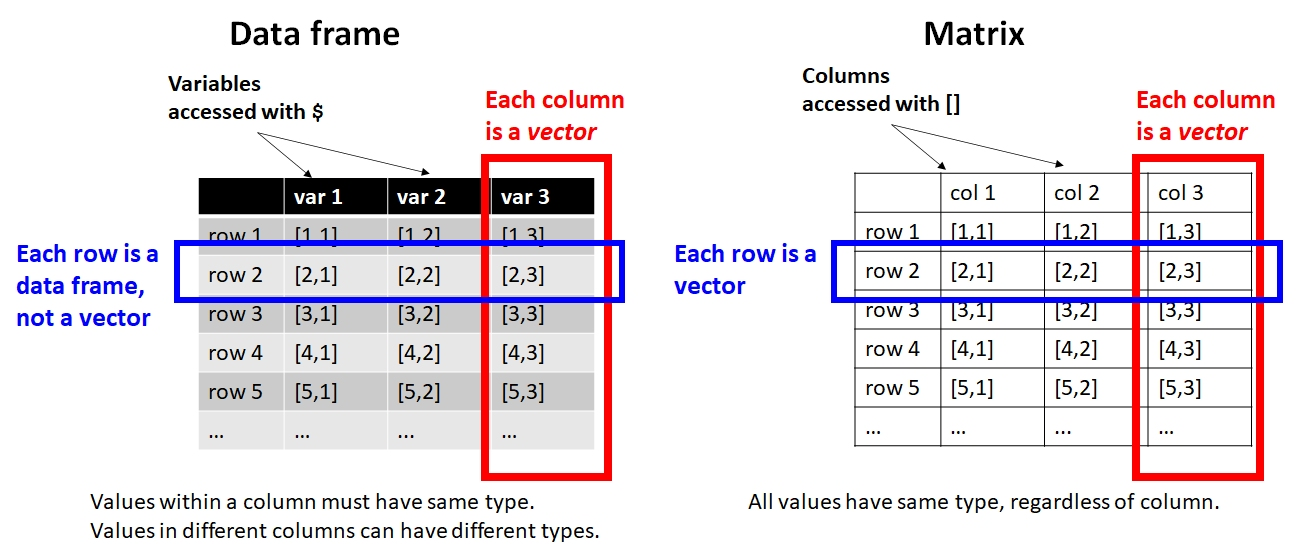
\includegraphics[keepaspectratio]{chapters/../images/05_08.jpg}}

}

\end{figure}%

When using \href{@sec-manip-select-bas}{bracket notation}, accessing
parts of a data frame is the same as for a matrix. There are a couple of
differences though:

\begin{itemize}
\item
  Matrices do not need column names, but data frames do. They are
  accessed with \texttt{colnames()} for matrices, but \texttt{names()}
  for data frames.
\item
  Columns of a data frame can be called with \texttt{\$}; e.g.,
  \texttt{iris\$Petal.Length}. The equivalent for a matrix would be
  \texttt{iris{[},"Petal.Length"{]}}. The \texttt{\$} works for data
  frames only, while the brackets method works for both data frames and
  matrices.
\end{itemize}

Here are some common methods of accessing values in a data frame:

\begin{Shaded}
\begin{Highlighting}[]

\CommentTok{\# single variables (columns): $}
\NormalTok{iris}\SpecialCharTok{$}\NormalTok{Petal.Length}
\DocumentationTok{\#\#   [1] 1.4 1.4 1.3 1.5 1.4 1.7 1.4 1.5 1.4 1.5 1.5 1.6 1.4 1.1 1.2 1.5 1.3 1.4}
\DocumentationTok{\#\#  [19] 1.7 1.5 1.7 1.5 1.0 1.7 1.9 1.6 1.6 1.5 1.4 1.6 1.6 1.5 1.5 1.4 1.5 1.2}
\DocumentationTok{\#\#  [37] 1.3 1.4 1.3 1.5 1.3 1.3 1.3 1.6 1.9 1.4 1.6 1.4 1.5 1.4 4.7 4.5 4.9 4.0}
\DocumentationTok{\#\#  [55] 4.6 4.5 4.7 3.3 4.6 3.9 3.5 4.2 4.0 4.7 3.6 4.4 4.5 4.1 4.5 3.9 4.8 4.0}
\DocumentationTok{\#\#  [73] 4.9 4.7 4.3 4.4 4.8 5.0 4.5 3.5 3.8 3.7 3.9 5.1 4.5 4.5 4.7 4.4 4.1 4.0}
\DocumentationTok{\#\#  [91] 4.4 4.6 4.0 3.3 4.2 4.2 4.2 4.3 3.0 4.1 6.0 5.1 5.9 5.6 5.8 6.6 4.5 6.3}
\DocumentationTok{\#\# [109] 5.8 6.1 5.1 5.3 5.5 5.0 5.1 5.3 5.5 6.7 6.9 5.0 5.7 4.9 6.7 4.9 5.7 6.0}
\DocumentationTok{\#\# [127] 4.8 4.9 5.6 5.8 6.1 6.4 5.6 5.1 5.6 6.1 5.6 5.5 4.8 5.4 5.6 5.1 5.1 5.9}
\DocumentationTok{\#\# [145] 5.7 5.2 5.0 5.2 5.4 5.1}

\CommentTok{\# multiple variables: brackets []}
\DocumentationTok{\#\# head() shows only first few rows (output very long)}
\NormalTok{a }\OtherTok{\textless{}{-}}\NormalTok{ iris[,}\FunctionTok{c}\NormalTok{(}\StringTok{"Petal.Length"}\NormalTok{, }\StringTok{"Sepal.Length"}\NormalTok{)]}
\FunctionTok{head}\NormalTok{(a)}
\DocumentationTok{\#\#   Petal.Length Sepal.Length}
\DocumentationTok{\#\# 1          1.4          5.1}
\DocumentationTok{\#\# 2          1.4          4.9}
\DocumentationTok{\#\# 3          1.3          4.7}
\DocumentationTok{\#\# 4          1.5          4.6}
\DocumentationTok{\#\# 5          1.4          5.0}
\DocumentationTok{\#\# 6          1.7          5.4}

\CommentTok{\# rows: brackets []}
\CommentTok{\# remember the comma!}
\NormalTok{iris[}\DecValTok{1}\SpecialCharTok{:}\DecValTok{4}\NormalTok{,]}
\DocumentationTok{\#\#   Sepal.Length Sepal.Width Petal.Length Petal.Width Species}
\DocumentationTok{\#\# 1          5.1         3.5          1.4         0.2  setosa}
\DocumentationTok{\#\# 2          4.9         3.0          1.4         0.2  setosa}
\DocumentationTok{\#\# 3          4.7         3.2          1.3         0.2  setosa}
\DocumentationTok{\#\# 4          4.6         3.1          1.5         0.2  setosa}
\NormalTok{iris[}\DecValTok{1}\NormalTok{,]}
\DocumentationTok{\#\#   Sepal.Length Sepal.Width Petal.Length Petal.Width Species}
\DocumentationTok{\#\# 1          5.1         3.5          1.4         0.2  setosa}
\end{Highlighting}
\end{Shaded}

When a data frame is printed to the console, this is only a
representation of the data frame's true form: a \textbf{list}. This is
why single columns are accessible by a \texttt{\$}: this is the symbol
for accessing an element of a list. The list nature of a data frame is
also why \textbf{rows} of a dataset are actually data frames themselves
and not vectors.

\subsection{Common operations}\label{sec-manip-df-com}

\subsubsection{Adding and deleting
variables}\label{sec-manip-df-com-vars}

New variables can be added to a data frame by \textbf{assignment}
(\texttt{\textless{}-}). Assigning values to a variable in a data frame
will create that variable if it doesn't already exist--and overwrite
values if the variable is already in the data frame.

\begin{Shaded}
\begin{Highlighting}[]
\CommentTok{\# spare copy with just a }
\CommentTok{\# few rows for demonstration}
\NormalTok{x }\OtherTok{\textless{}{-}}\NormalTok{ iris[}\DecValTok{1}\SpecialCharTok{:}\DecValTok{5}\NormalTok{,] }

\CommentTok{\# make a new column with \textless{}{-}}
\NormalTok{x}\SpecialCharTok{$}\NormalTok{Petal.Area }\OtherTok{\textless{}{-}} \FunctionTok{apply}\NormalTok{(x[,}\DecValTok{3}\SpecialCharTok{:}\DecValTok{4}\NormalTok{], }\DecValTok{1}\NormalTok{, prod)}

\CommentTok{\# shows data frame with new variable:}
\NormalTok{x}
\DocumentationTok{\#\#   Sepal.Length Sepal.Width Petal.Length Petal.Width Species Petal.Area}
\DocumentationTok{\#\# 1          5.1         3.5          1.4         0.2  setosa       0.28}
\DocumentationTok{\#\# 2          4.9         3.0          1.4         0.2  setosa       0.28}
\DocumentationTok{\#\# 3          4.7         3.2          1.3         0.2  setosa       0.26}
\DocumentationTok{\#\# 4          4.6         3.1          1.5         0.2  setosa       0.30}
\DocumentationTok{\#\# 5          5.0         3.6          1.4         0.2  setosa       0.28}

\CommentTok{\# overwrite the new variable}
\NormalTok{x}\SpecialCharTok{$}\NormalTok{Petal.Area }\OtherTok{\textless{}{-}} \DecValTok{3}
\NormalTok{x}
\DocumentationTok{\#\#   Sepal.Length Sepal.Width Petal.Length Petal.Width Species Petal.Area}
\DocumentationTok{\#\# 1          5.1         3.5          1.4         0.2  setosa          3}
\DocumentationTok{\#\# 2          4.9         3.0          1.4         0.2  setosa          3}
\DocumentationTok{\#\# 3          4.7         3.2          1.3         0.2  setosa          3}
\DocumentationTok{\#\# 4          4.6         3.1          1.5         0.2  setosa          3}
\DocumentationTok{\#\# 5          5.0         3.6          1.4         0.2  setosa          3}
\end{Highlighting}
\end{Shaded}

Variables can also be added using function \texttt{cbind()}. This name
is short for ``column bind''\textasciitilde{[}\texttt{cbind()} works on
matrices too.{]}. To use \texttt{cbind()}, the input data frames must
have the same number of rows. Note that \texttt{cbind()} sticks the data
frames together as they are. If the records in the inputs need to be
matched up and are not already in the same order, then either the data
frames need to be aligned, merged with function \texttt{merge()}, or the
variables need to be added using \texttt{match()} and a key variable.

\begin{Shaded}
\begin{Highlighting}[]
\CommentTok{\# make 2 data frames where rows line up}
\NormalTok{x }\OtherTok{\textless{}{-}}\NormalTok{ iris[}\DecValTok{1}\SpecialCharTok{:}\DecValTok{5}\NormalTok{, }\DecValTok{1}\SpecialCharTok{:}\DecValTok{2}\NormalTok{]}
\NormalTok{y }\OtherTok{\textless{}{-}}\NormalTok{ iris[}\DecValTok{1}\SpecialCharTok{:}\DecValTok{5}\NormalTok{, }\DecValTok{3}\SpecialCharTok{:}\DecValTok{5}\NormalTok{]}
\FunctionTok{cbind}\NormalTok{(x,y)}
\DocumentationTok{\#\#   Sepal.Length Sepal.Width Petal.Length Petal.Width Species}
\DocumentationTok{\#\# 1          5.1         3.5          1.4         0.2  setosa}
\DocumentationTok{\#\# 2          4.9         3.0          1.4         0.2  setosa}
\DocumentationTok{\#\# 3          4.7         3.2          1.3         0.2  setosa}
\DocumentationTok{\#\# 4          4.6         3.1          1.5         0.2  setosa}
\DocumentationTok{\#\# 5          5.0         3.6          1.4         0.2  setosa}

\CommentTok{\# shows that cbind() uses inputs as{-}is}
\CommentTok{\# and makes no attempt at matching.}
\FunctionTok{cbind}\NormalTok{(x, y[}\DecValTok{5}\SpecialCharTok{:}\DecValTok{1}\NormalTok{,])}
\DocumentationTok{\#\#   Sepal.Length Sepal.Width Petal.Length Petal.Width Species}
\DocumentationTok{\#\# 1          5.1         3.5          1.4         0.2  setosa}
\DocumentationTok{\#\# 2          4.9         3.0          1.5         0.2  setosa}
\DocumentationTok{\#\# 3          4.7         3.2          1.3         0.2  setosa}
\DocumentationTok{\#\# 4          4.6         3.1          1.4         0.2  setosa}
\DocumentationTok{\#\# 5          5.0         3.6          1.4         0.2  setosa}
\end{Highlighting}
\end{Shaded}

Variables can be deleted by setting them to \texttt{NULL} (notice all
caps) or by making a new version of the data frame without the variable.
If I am only removing a few variables, I prefer setting them
individually to NULL. This makes it less likely that I will accidentally
remove the wrong columns.

\begin{Shaded}
\begin{Highlighting}[]
\CommentTok{\# delete this variable}
\NormalTok{z }\OtherTok{\textless{}{-}}\NormalTok{ x}
\NormalTok{z}\SpecialCharTok{$}\NormalTok{Petal.Area }\OtherTok{\textless{}{-}} \ConstantTok{NULL}
\NormalTok{z}
\DocumentationTok{\#\#   Sepal.Length Sepal.Width}
\DocumentationTok{\#\# 1          5.1         3.5}
\DocumentationTok{\#\# 2          4.9         3.0}
\DocumentationTok{\#\# 3          4.7         3.2}
\DocumentationTok{\#\# 4          4.6         3.1}
\DocumentationTok{\#\# 5          5.0         3.6}

\CommentTok{\# delete 1 variable with brackets}
\NormalTok{z }\OtherTok{\textless{}{-}}\NormalTok{ x}
\NormalTok{z }\OtherTok{\textless{}{-}}\NormalTok{ z[,}\FunctionTok{which}\NormalTok{(}\FunctionTok{names}\NormalTok{(z) }\SpecialCharTok{!=} \StringTok{"Petal.Area"}\NormalTok{)]}
\NormalTok{z}
\DocumentationTok{\#\#   Sepal.Length Sepal.Width}
\DocumentationTok{\#\# 1          5.1         3.5}
\DocumentationTok{\#\# 2          4.9         3.0}
\DocumentationTok{\#\# 3          4.7         3.2}
\DocumentationTok{\#\# 4          4.6         3.1}
\DocumentationTok{\#\# 5          5.0         3.6}

\CommentTok{\# delete \textgreater{}1 variable}
\NormalTok{z }\OtherTok{\textless{}{-}}\NormalTok{ x}
\NormalTok{del.cols }\OtherTok{\textless{}{-}} \FunctionTok{c}\NormalTok{(}\StringTok{"Petal.Area"}\NormalTok{, }\StringTok{"Petal.Length"}\NormalTok{)}
\NormalTok{z }\OtherTok{\textless{}{-}}\NormalTok{ z[,}\FunctionTok{which}\NormalTok{(}\SpecialCharTok{!}\FunctionTok{names}\NormalTok{(z) }\SpecialCharTok{\%in\%}\NormalTok{ del.cols)]}
\NormalTok{z}
\DocumentationTok{\#\#   Sepal.Length Sepal.Width}
\DocumentationTok{\#\# 1          5.1         3.5}
\DocumentationTok{\#\# 2          4.9         3.0}
\DocumentationTok{\#\# 3          4.7         3.2}
\DocumentationTok{\#\# 4          4.6         3.1}
\DocumentationTok{\#\# 5          5.0         3.6}
\end{Highlighting}
\end{Shaded}

\subsubsection{Modifying variables}\label{sec-manip-df-com-mod}

Variables in a data frame (or anywhere) can be modified by assigning
them new values. Note that this overwrites the previous values. If you
think you might want the old values for some reason, save the modified
values in a new variable or even new object instead.

\begin{Shaded}
\begin{Highlighting}[]
\CommentTok{\# not run}

\CommentTok{\# spare copy with just a }
\CommentTok{\# few rows for demonstration}
\NormalTok{x }\OtherTok{\textless{}{-}}\NormalTok{ iris[}\DecValTok{1}\SpecialCharTok{:}\DecValTok{5}\NormalTok{,] }
\NormalTok{x}\SpecialCharTok{$}\NormalTok{Petal.Length }\OtherTok{\textless{}{-}} \FunctionTok{log}\NormalTok{(x}\SpecialCharTok{$}\NormalTok{Petal.Length)}

\CommentTok{\# better: keep modified values in new variable}

\CommentTok{\# spare copy with just a }
\CommentTok{\# few rows for demonstration}
\NormalTok{x }\OtherTok{\textless{}{-}}\NormalTok{ iris[}\DecValTok{1}\SpecialCharTok{:}\DecValTok{5}\NormalTok{,] }
\NormalTok{x}\SpecialCharTok{$}\NormalTok{log.petlen }\OtherTok{\textless{}{-}} \FunctionTok{log}\NormalTok{(x}\SpecialCharTok{$}\NormalTok{Petal.Length)}
\end{Highlighting}
\end{Shaded}

\subsubsection{Changing values using a
rule}\label{sec-manip-df-com-rule}

By combining the logical tests, bracket notation, and assignment, values
in a variable can be replaced according to their values.

\begin{Shaded}
\begin{Highlighting}[]
\CommentTok{\# not run (long output), but try it on your machine!}
\NormalTok{x }\OtherTok{\textless{}{-}}\NormalTok{ iris}

\CommentTok{\# select and replace by one condition:}
\NormalTok{flag }\OtherTok{\textless{}{-}} \FunctionTok{which}\NormalTok{(x}\SpecialCharTok{$}\NormalTok{Sepal.Length }\SpecialCharTok{\textgreater{}=} \DecValTok{6}\NormalTok{)}
\NormalTok{x}\SpecialCharTok{$}\NormalTok{Sepal.Length[flag] }\OtherTok{\textless{}{-}} \FloatTok{5.99}
\NormalTok{x}

\CommentTok{\# select and replace by 2 conditions:}
\NormalTok{flag1 }\OtherTok{\textless{}{-}} \FunctionTok{which}\NormalTok{(x}\SpecialCharTok{$}\NormalTok{Petal.Length }\SpecialCharTok{\textgreater{}=} \DecValTok{3}\NormalTok{)}
\NormalTok{flag2 }\OtherTok{\textless{}{-}} \FunctionTok{which}\NormalTok{(x}\SpecialCharTok{$}\NormalTok{Petal.Length }\SpecialCharTok{\textless{}=} \DecValTok{5}\NormalTok{)}
\NormalTok{x}\SpecialCharTok{$}\NormalTok{Petal.Length[}\FunctionTok{intersect}\NormalTok{(flag1, flag2)] }\OtherTok{\textless{}{-}} \DecValTok{4}
\NormalTok{x}

\CommentTok{\# equivalent to above, but with \&}
\NormalTok{flag1 }\OtherTok{\textless{}{-}} \FunctionTok{which}\NormalTok{(x}\SpecialCharTok{$}\NormalTok{Petal.Length }\SpecialCharTok{\textgreater{}=} \DecValTok{3}\NormalTok{)}
\NormalTok{flag2 }\OtherTok{\textless{}{-}} \FunctionTok{which}\NormalTok{(x}\SpecialCharTok{$}\NormalTok{Petal.Length }\SpecialCharTok{\textless{}=} \DecValTok{5}\NormalTok{)}
\NormalTok{x}\SpecialCharTok{$}\NormalTok{Petal.Length[flag1 }\SpecialCharTok{\&}\NormalTok{ flag2] }\OtherTok{\textless{}{-}} \DecValTok{4}
\NormalTok{x}
\end{Highlighting}
\end{Shaded}

\subsubsection{Renaming variables}\label{sec-manip-df-com-renam}

Renaming variables in Excel is easy: just enter the new name into the
cell at the top of a column. Things are a little more complicated in R
but not much.

There are a few ways to rename columns, and they all involve accessing
the variable names using function \texttt{names()}.

\begin{Shaded}
\begin{Highlighting}[]

\CommentTok{\# spare copy with just a }
\CommentTok{\# few rows for demonstration}
\NormalTok{x }\OtherTok{\textless{}{-}}\NormalTok{ iris[}\DecValTok{1}\SpecialCharTok{:}\DecValTok{5}\NormalTok{,] }

\CommentTok{\# rname by column number:}
\FunctionTok{names}\NormalTok{(x)[}\DecValTok{1}\NormalTok{] }\OtherTok{\textless{}{-}} \StringTok{"sep.len"}
\NormalTok{x}
\DocumentationTok{\#\#   sep.len Sepal.Width Petal.Length Petal.Width Species}
\DocumentationTok{\#\# 1     5.1         3.5          1.4         0.2  setosa}
\DocumentationTok{\#\# 2     4.9         3.0          1.4         0.2  setosa}
\DocumentationTok{\#\# 3     4.7         3.2          1.3         0.2  setosa}
\DocumentationTok{\#\# 4     4.6         3.1          1.5         0.2  setosa}
\DocumentationTok{\#\# 5     5.0         3.6          1.4         0.2  setosa}

\CommentTok{\# match name exactly:}
\FunctionTok{names}\NormalTok{(x)[}\FunctionTok{which}\NormalTok{(}\FunctionTok{names}\NormalTok{(x) }\SpecialCharTok{==} \StringTok{"Petal.Length"}\NormalTok{)] }\OtherTok{\textless{}{-}} \StringTok{"pet.len"}
\NormalTok{x}
\DocumentationTok{\#\#   sep.len Sepal.Width pet.len Petal.Width Species}
\DocumentationTok{\#\# 1     5.1         3.5     1.4         0.2  setosa}
\DocumentationTok{\#\# 2     4.9         3.0     1.4         0.2  setosa}
\DocumentationTok{\#\# 3     4.7         3.2     1.3         0.2  setosa}
\DocumentationTok{\#\# 4     4.6         3.1     1.5         0.2  setosa}
\DocumentationTok{\#\# 5     5.0         3.6     1.4         0.2  setosa}

\CommentTok{\# equivalent, but separate search and action}
\NormalTok{flag }\OtherTok{\textless{}{-}} \FunctionTok{which}\NormalTok{(}\FunctionTok{names}\NormalTok{(x) }\SpecialCharTok{==} \StringTok{"Petal.Width"}\NormalTok{)}
\FunctionTok{names}\NormalTok{(x)[flag] }\OtherTok{\textless{}{-}} \StringTok{"pet.wid"}
\NormalTok{x}
\DocumentationTok{\#\#   sep.len Sepal.Width pet.len pet.wid Species}
\DocumentationTok{\#\# 1     5.1         3.5     1.4     0.2  setosa}
\DocumentationTok{\#\# 2     4.9         3.0     1.4     0.2  setosa}
\DocumentationTok{\#\# 3     4.7         3.2     1.3     0.2  setosa}
\DocumentationTok{\#\# 4     4.6         3.1     1.5     0.2  setosa}
\DocumentationTok{\#\# 5     5.0         3.6     1.4     0.2  setosa}

\CommentTok{\# by position:}
\FunctionTok{names}\NormalTok{(x)[}\FunctionTok{ncol}\NormalTok{(x)] }\OtherTok{\textless{}{-}} \StringTok{"species"}
\NormalTok{x}
\DocumentationTok{\#\#   sep.len Sepal.Width pet.len pet.wid species}
\DocumentationTok{\#\# 1     5.1         3.5     1.4     0.2  setosa}
\DocumentationTok{\#\# 2     4.9         3.0     1.4     0.2  setosa}
\DocumentationTok{\#\# 3     4.7         3.2     1.3     0.2  setosa}
\DocumentationTok{\#\# 4     4.6         3.1     1.5     0.2  setosa}
\DocumentationTok{\#\# 5     5.0         3.6     1.4     0.2  setosa}

\FunctionTok{names}\NormalTok{(x)[}\DecValTok{1}\NormalTok{] }\OtherTok{\textless{}{-}} \StringTok{"sepal.len"}
\NormalTok{x}
\DocumentationTok{\#\#   sepal.len Sepal.Width pet.len pet.wid species}
\DocumentationTok{\#\# 1       5.1         3.5     1.4     0.2  setosa}
\DocumentationTok{\#\# 2       4.9         3.0     1.4     0.2  setosa}
\DocumentationTok{\#\# 3       4.7         3.2     1.3     0.2  setosa}
\DocumentationTok{\#\# 4       4.6         3.1     1.5     0.2  setosa}
\DocumentationTok{\#\# 5       5.0         3.6     1.4     0.2  setosa}

\CommentTok{\# change several names at once:}
\FunctionTok{names}\NormalTok{(x)[}\DecValTok{1}\SpecialCharTok{:}\DecValTok{4}\NormalTok{] }\OtherTok{\textless{}{-}} \FunctionTok{paste0}\NormalTok{(}\StringTok{"x"}\NormalTok{, }\DecValTok{1}\SpecialCharTok{:}\DecValTok{4}\NormalTok{)}
\NormalTok{x}
\DocumentationTok{\#\#    x1  x2  x3  x4 species}
\DocumentationTok{\#\# 1 5.1 3.5 1.4 0.2  setosa}
\DocumentationTok{\#\# 2 4.9 3.0 1.4 0.2  setosa}
\DocumentationTok{\#\# 3 4.7 3.2 1.3 0.2  setosa}
\DocumentationTok{\#\# 4 4.6 3.1 1.5 0.2  setosa}
\DocumentationTok{\#\# 5 5.0 3.6 1.4 0.2  setosa}
\end{Highlighting}
\end{Shaded}

Finally, if you have a a lot of time on your hands, you can make a new
copy of the variable with the name you want, then delete the original
version. This has the disadvantage of changing the order of columns.

\begin{Shaded}
\begin{Highlighting}[]
\NormalTok{x }\OtherTok{\textless{}{-}}\NormalTok{ iris[}\DecValTok{1}\SpecialCharTok{:}\DecValTok{5}\NormalTok{,] }\CommentTok{\# spare copy for demonstration}
\NormalTok{x}\SpecialCharTok{$}\NormalTok{pet.len }\OtherTok{\textless{}{-}}\NormalTok{ x}\SpecialCharTok{$}\NormalTok{Petal.Length}
\NormalTok{x}\SpecialCharTok{$}\NormalTok{Petal.Length }\OtherTok{\textless{}{-}} \ConstantTok{NULL}
\NormalTok{x}
\end{Highlighting}
\end{Shaded}

\begin{verbatim}
  Sepal.Length Sepal.Width Petal.Width Species pet.len
1          5.1         3.5         0.2  setosa     1.4
2          4.9         3.0         0.2  setosa     1.4
3          4.7         3.2         0.2  setosa     1.3
4          4.6         3.1         0.2  setosa     1.5
5          5.0         3.6         0.2  setosa     1.4
\end{verbatim}

\subsubsection{Rearranging columns}\label{sec-manip-df-com-rearr}

Reordering records or columns within a data frame is accomplished by
creating a new version of the dataset with the desired arrangement. This
rearrangement is accomplished using methods we have already seen.

\begin{Shaded}
\begin{Highlighting}[]

\CommentTok{\# spare copy with just a }
\CommentTok{\# few rows for demonstration}
\NormalTok{x }\OtherTok{\textless{}{-}}\NormalTok{ iris[}\DecValTok{1}\SpecialCharTok{:}\DecValTok{5}\NormalTok{,] }

\CommentTok{\# rearrange by number}
\NormalTok{x }\OtherTok{\textless{}{-}}\NormalTok{ x[,}\FunctionTok{c}\NormalTok{(}\DecValTok{5}\NormalTok{, }\DecValTok{3}\NormalTok{, }\DecValTok{4}\NormalTok{, }\DecValTok{1}\NormalTok{, }\DecValTok{2}\NormalTok{)]}
\NormalTok{x}
\DocumentationTok{\#\#   Species Petal.Length Petal.Width Sepal.Length Sepal.Width}
\DocumentationTok{\#\# 1  setosa          1.4         0.2          5.1         3.5}
\DocumentationTok{\#\# 2  setosa          1.4         0.2          4.9         3.0}
\DocumentationTok{\#\# 3  setosa          1.3         0.2          4.7         3.2}
\DocumentationTok{\#\# 4  setosa          1.5         0.2          4.6         3.1}
\DocumentationTok{\#\# 5  setosa          1.4         0.2          5.0         3.6}

\CommentTok{\# rearrange by name}
\NormalTok{col.order }\OtherTok{\textless{}{-}} \FunctionTok{c}\NormalTok{(}\StringTok{"Species"}\NormalTok{, }\StringTok{"Sepal.Length"}\NormalTok{, }\StringTok{"Sepal.Width"}\NormalTok{, }
               \StringTok{"Petal.Length"}\NormalTok{, }\StringTok{"Petal.Width"}\NormalTok{)}
\NormalTok{x }\OtherTok{\textless{}{-}}\NormalTok{ x[,col.order]}
\NormalTok{x}
\DocumentationTok{\#\#   Species Sepal.Length Sepal.Width Petal.Length Petal.Width}
\DocumentationTok{\#\# 1  setosa          5.1         3.5          1.4         0.2}
\DocumentationTok{\#\# 2  setosa          4.9         3.0          1.4         0.2}
\DocumentationTok{\#\# 3  setosa          4.7         3.2          1.3         0.2}
\DocumentationTok{\#\# 4  setosa          4.6         3.1          1.5         0.2}
\DocumentationTok{\#\# 5  setosa          5.0         3.6          1.4         0.2}
\end{Highlighting}
\end{Shaded}

\subsubsection{Sorting and ordering data}\label{sec-manip-df-com-sort}

Sorting data frames is mostly done using the function \texttt{order()}
(function \texttt{sort()} works on vectors, not data frames). Function
\texttt{order()} is usually put inside brackets in the rows slot. The
arguments to \texttt{order()} define the variables by which the data
frame will be sorted. Rows are sorted by the first variable, then the
second, and so on. By default, rows are placed in \emph{ascending}
order.

Use \texttt{sort()} on vectors:

\begin{Shaded}
\begin{Highlighting}[]
\CommentTok{\# values 1:12 in random order}
\FunctionTok{set.seed}\NormalTok{(}\DecValTok{123}\NormalTok{)}
\NormalTok{w }\OtherTok{\textless{}{-}} \FunctionTok{sample}\NormalTok{(}\DecValTok{1}\SpecialCharTok{:}\DecValTok{12}\NormalTok{, }\DecValTok{12}\NormalTok{, }\AttributeTok{replace=}\ConstantTok{FALSE}\NormalTok{)}
\NormalTok{w}
\DocumentationTok{\#\#  [1]  3 12 10  2  6 11  5  4  9  8  1  7}

\CommentTok{\# sort ascending}
\NormalTok{w.inc }\OtherTok{\textless{}{-}} \FunctionTok{sort}\NormalTok{(w)}
\NormalTok{w.inc}
\DocumentationTok{\#\#  [1]  1  2  3  4  5  6  7  8  9 10 11 12}

\CommentTok{\# sort descending:}
\NormalTok{w.dec1 }\OtherTok{\textless{}{-}} \FunctionTok{sort}\NormalTok{(w, }\AttributeTok{decreasing=}\ConstantTok{TRUE}\NormalTok{)}
\DocumentationTok{\#\# or:}
\NormalTok{w.dec2 }\OtherTok{\textless{}{-}} \FunctionTok{rev}\NormalTok{(}\FunctionTok{sort}\NormalTok{(w))}
\NormalTok{w.dec1}
\DocumentationTok{\#\#  [1] 12 11 10  9  8  7  6  5  4  3  2  1}
\NormalTok{w.dec2}
\DocumentationTok{\#\#  [1] 12 11 10  9  8  7  6  5  4  3  2  1}
\end{Highlighting}
\end{Shaded}

One of my favorite uses of \texttt{sort()} is to get the unique values
of a vector in ascending (especially alphabetical) order.

\begin{Shaded}
\begin{Highlighting}[]
\CommentTok{\# get 100 random letters from a:e}
\NormalTok{a }\OtherTok{\textless{}{-}} \FunctionTok{sample}\NormalTok{(letters[}\DecValTok{1}\SpecialCharTok{:}\DecValTok{5}\NormalTok{], }\DecValTok{30}\NormalTok{, }\AttributeTok{replace=}\ConstantTok{TRUE}\NormalTok{)}
\NormalTok{a}
\DocumentationTok{\#\#  [1] "c" "e" "c" "c" "a" "d" "a" "a" "e" "c" "b" "b" "a" "c" "d" "a" "c" "e" "d"}
\DocumentationTok{\#\# [20] "b" "e" "a" "a" "b" "c" "d" "e" "e" "c" "a"}

\CommentTok{\# get the unique values, in alpha order}
\NormalTok{a.uniq }\OtherTok{\textless{}{-}} \FunctionTok{sort}\NormalTok{(}\FunctionTok{unique}\NormalTok{(a))}
\NormalTok{a.uniq}
\DocumentationTok{\#\# [1] "a" "b" "c" "d" "e"}
\end{Highlighting}
\end{Shaded}

Using \texttt{order()} on a data fame is similar to running 1 or more
\texttt{sort()} commands, but where \texttt{sort()} returns the sorted
vector, \texttt{order()} actually returns the indices of the sorted
object.

\begin{Shaded}
\begin{Highlighting}[]
\CommentTok{\# 6 random rows of iris:}
\FunctionTok{set.seed}\NormalTok{(}\DecValTok{124}\NormalTok{)}
\NormalTok{z }\OtherTok{\textless{}{-}}\NormalTok{ iris[}\FunctionTok{sample}\NormalTok{(}\DecValTok{1}\SpecialCharTok{:}\FunctionTok{nrow}\NormalTok{(iris), }\DecValTok{6}\NormalTok{),]}
\NormalTok{z}
\end{Highlighting}
\end{Shaded}

\begin{verbatim}
    Sepal.Length Sepal.Width Petal.Length Petal.Width    Species
65           5.6         2.9          3.6         1.3 versicolor
5            5.0         3.6          1.4         0.2     setosa
134          6.3         2.8          5.1         1.5  virginica
74           6.1         2.8          4.7         1.2 versicolor
143          5.8         2.7          5.1         1.9  virginica
91           5.5         2.6          4.4         1.2 versicolor
\end{verbatim}

\begin{Shaded}
\begin{Highlighting}[]
\CommentTok{\# order z by increasing Petal.Length}

\DocumentationTok{\#\# returns indices}
\FunctionTok{order}\NormalTok{(z}\SpecialCharTok{$}\NormalTok{Petal.Length)}
\end{Highlighting}
\end{Shaded}

\begin{verbatim}
[1] 2 1 6 4 3 5
\end{verbatim}

\begin{Shaded}
\begin{Highlighting}[]
\DocumentationTok{\#\# uses those indices in []}
\DocumentationTok{\#\# to produce sorted data frame}
\NormalTok{z[}\FunctionTok{order}\NormalTok{(z}\SpecialCharTok{$}\NormalTok{Petal.Length),]}
\end{Highlighting}
\end{Shaded}

\begin{verbatim}
    Sepal.Length Sepal.Width Petal.Length Petal.Width    Species
5            5.0         3.6          1.4         0.2     setosa
65           5.6         2.9          3.6         1.3 versicolor
91           5.5         2.6          4.4         1.2 versicolor
74           6.1         2.8          4.7         1.2 versicolor
134          6.3         2.8          5.1         1.5  virginica
143          5.8         2.7          5.1         1.9  virginica
\end{verbatim}

\begin{Shaded}
\begin{Highlighting}[]
\DocumentationTok{\#\# order by species (alphabetical ascending), }
\DocumentationTok{\#\#  then by petal length (ascending)}
\NormalTok{z[}\FunctionTok{order}\NormalTok{(z}\SpecialCharTok{$}\NormalTok{Species, z}\SpecialCharTok{$}\NormalTok{Petal.Length),]}
\end{Highlighting}
\end{Shaded}

\begin{verbatim}
    Sepal.Length Sepal.Width Petal.Length Petal.Width    Species
5            5.0         3.6          1.4         0.2     setosa
65           5.6         2.9          3.6         1.3 versicolor
91           5.5         2.6          4.4         1.2 versicolor
74           6.1         2.8          4.7         1.2 versicolor
134          6.3         2.8          5.1         1.5  virginica
143          5.8         2.7          5.1         1.9  virginica
\end{verbatim}

You can multiple variables to \texttt{order()}, by name, and R will
order the rows in each variable in the order supplied. By default,
records are sorted in ascending order. If you want a mix of ascending
and descending order, you have to specify the \texttt{radix} method and
specify whether you want the order to be decreasing (TRUE) or not
(FALSE) for each variable:

\begin{Shaded}
\begin{Highlighting}[]
\CommentTok{\# sort alpha by species, then}
\CommentTok{\# by decreasing petal length}
\NormalTok{z[}\FunctionTok{order}\NormalTok{(z}\SpecialCharTok{$}\NormalTok{Species, z}\SpecialCharTok{$}\NormalTok{Petal.Length, }
           \AttributeTok{decreasing=}\FunctionTok{c}\NormalTok{(}\ConstantTok{TRUE}\NormalTok{, }\ConstantTok{FALSE}\NormalTok{),}
           \AttributeTok{method=}\StringTok{"radix"}\NormalTok{),]}
\end{Highlighting}
\end{Shaded}

\subsubsection{Adding and removing rows}\label{sec-manip-df-com-add}

Removing rows works a lot like removing columns. You can use the bracket
notation to either remove the rows with negative indices, or make a new
version of the data frame with only some of the rows.

\begin{Shaded}
\begin{Highlighting}[]
\CommentTok{\# spare copy with just a }
\CommentTok{\# few rows for demonstration}
\NormalTok{x }\OtherTok{\textless{}{-}}\NormalTok{ iris[}\DecValTok{1}\SpecialCharTok{:}\DecValTok{10}\NormalTok{,] }

\CommentTok{\# remove rows by their number}
\NormalTok{x[}\SpecialCharTok{{-}}\DecValTok{1}\NormalTok{,]}
\DocumentationTok{\#\#    Sepal.Length Sepal.Width Petal.Length Petal.Width Species}
\DocumentationTok{\#\# 2           4.9         3.0          1.4         0.2  setosa}
\DocumentationTok{\#\# 3           4.7         3.2          1.3         0.2  setosa}
\DocumentationTok{\#\# 4           4.6         3.1          1.5         0.2  setosa}
\DocumentationTok{\#\# 5           5.0         3.6          1.4         0.2  setosa}
\DocumentationTok{\#\# 6           5.4         3.9          1.7         0.4  setosa}
\DocumentationTok{\#\# 7           4.6         3.4          1.4         0.3  setosa}
\DocumentationTok{\#\# 8           5.0         3.4          1.5         0.2  setosa}
\DocumentationTok{\#\# 9           4.4         2.9          1.4         0.2  setosa}
\DocumentationTok{\#\# 10          4.9         3.1          1.5         0.1  setosa}
\NormalTok{x[}\SpecialCharTok{{-}}\FunctionTok{c}\NormalTok{(}\DecValTok{1}\SpecialCharTok{:}\DecValTok{3}\NormalTok{),]}
\DocumentationTok{\#\#    Sepal.Length Sepal.Width Petal.Length Petal.Width Species}
\DocumentationTok{\#\# 4           4.6         3.1          1.5         0.2  setosa}
\DocumentationTok{\#\# 5           5.0         3.6          1.4         0.2  setosa}
\DocumentationTok{\#\# 6           5.4         3.9          1.7         0.4  setosa}
\DocumentationTok{\#\# 7           4.6         3.4          1.4         0.3  setosa}
\DocumentationTok{\#\# 8           5.0         3.4          1.5         0.2  setosa}
\DocumentationTok{\#\# 9           4.4         2.9          1.4         0.2  setosa}
\DocumentationTok{\#\# 10          4.9         3.1          1.5         0.1  setosa}
\NormalTok{x[}\SpecialCharTok{{-}}\FunctionTok{c}\NormalTok{(}\DecValTok{1}\NormalTok{, }\DecValTok{3}\NormalTok{, }\DecValTok{5}\NormalTok{, }\DecValTok{7}\NormalTok{, }\DecValTok{9}\NormalTok{),]}
\DocumentationTok{\#\#    Sepal.Length Sepal.Width Petal.Length Petal.Width Species}
\DocumentationTok{\#\# 2           4.9         3.0          1.4         0.2  setosa}
\DocumentationTok{\#\# 4           4.6         3.1          1.5         0.2  setosa}
\DocumentationTok{\#\# 6           5.4         3.9          1.7         0.4  setosa}
\DocumentationTok{\#\# 8           5.0         3.4          1.5         0.2  setosa}
\DocumentationTok{\#\# 10          4.9         3.1          1.5         0.1  setosa}

\CommentTok{\# or, make a new copy with the }
\CommentTok{\# rows to keep}
\NormalTok{x[}\DecValTok{2}\SpecialCharTok{:}\DecValTok{10}\NormalTok{,]}
\DocumentationTok{\#\#    Sepal.Length Sepal.Width Petal.Length Petal.Width Species}
\DocumentationTok{\#\# 2           4.9         3.0          1.4         0.2  setosa}
\DocumentationTok{\#\# 3           4.7         3.2          1.3         0.2  setosa}
\DocumentationTok{\#\# 4           4.6         3.1          1.5         0.2  setosa}
\DocumentationTok{\#\# 5           5.0         3.6          1.4         0.2  setosa}
\DocumentationTok{\#\# 6           5.4         3.9          1.7         0.4  setosa}
\DocumentationTok{\#\# 7           4.6         3.4          1.4         0.3  setosa}
\DocumentationTok{\#\# 8           5.0         3.4          1.5         0.2  setosa}
\DocumentationTok{\#\# 9           4.4         2.9          1.4         0.2  setosa}
\DocumentationTok{\#\# 10          4.9         3.1          1.5         0.1  setosa}
\NormalTok{x[}\FunctionTok{c}\NormalTok{(}\DecValTok{2}\NormalTok{, }\DecValTok{4}\NormalTok{, }\DecValTok{6}\NormalTok{, }\DecValTok{8}\NormalTok{, }\DecValTok{10}\NormalTok{),]}
\DocumentationTok{\#\#    Sepal.Length Sepal.Width Petal.Length Petal.Width Species}
\DocumentationTok{\#\# 2           4.9         3.0          1.4         0.2  setosa}
\DocumentationTok{\#\# 4           4.6         3.1          1.5         0.2  setosa}
\DocumentationTok{\#\# 6           5.4         3.9          1.7         0.4  setosa}
\DocumentationTok{\#\# 8           5.0         3.4          1.5         0.2  setosa}
\DocumentationTok{\#\# 10          4.9         3.1          1.5         0.1  setosa}
\end{Highlighting}
\end{Shaded}

Adding rows can be done with \texttt{rbind()} (short for ``row bind'').
This function is analogous to \texttt{cbind()}, which joins objects by
their columns.

Adding rows to a data frame is tantamount to combining it with another
data frame. The data frames being combined \emph{must have the same
columns}, with the \emph{same names}, but the \emph{order of columns can
be different}.

\begin{Shaded}
\begin{Highlighting}[]

\NormalTok{x }\OtherTok{\textless{}{-}}\NormalTok{ iris[}\DecValTok{1}\SpecialCharTok{:}\DecValTok{5}\NormalTok{,]}
\NormalTok{y }\OtherTok{\textless{}{-}}\NormalTok{ iris[}\DecValTok{51}\SpecialCharTok{:}\DecValTok{55}\NormalTok{,]}

\CommentTok{\# columns match exactly:}
\FunctionTok{rbind}\NormalTok{(x, y)}
\DocumentationTok{\#\#    Sepal.Length Sepal.Width Petal.Length Petal.Width    Species}
\DocumentationTok{\#\# 1           5.1         3.5          1.4         0.2     setosa}
\DocumentationTok{\#\# 2           4.9         3.0          1.4         0.2     setosa}
\DocumentationTok{\#\# 3           4.7         3.2          1.3         0.2     setosa}
\DocumentationTok{\#\# 4           4.6         3.1          1.5         0.2     setosa}
\DocumentationTok{\#\# 5           5.0         3.6          1.4         0.2     setosa}
\DocumentationTok{\#\# 51          7.0         3.2          4.7         1.4 versicolor}
\DocumentationTok{\#\# 52          6.4         3.2          4.5         1.5 versicolor}
\DocumentationTok{\#\# 53          6.9         3.1          4.9         1.5 versicolor}
\DocumentationTok{\#\# 54          5.5         2.3          4.0         1.3 versicolor}
\DocumentationTok{\#\# 55          6.5         2.8          4.6         1.5 versicolor}

\CommentTok{\# columns in different order}
\CommentTok{\# is still ok, but rbinding}
\CommentTok{\# without making column orders}
\CommentTok{\# match makes me nervous.}
\NormalTok{y2 }\OtherTok{\textless{}{-}}\NormalTok{ y[,}\FunctionTok{c}\NormalTok{(}\DecValTok{3}\NormalTok{,}\DecValTok{5}\NormalTok{,}\DecValTok{2}\NormalTok{,}\DecValTok{1}\NormalTok{,}\DecValTok{4}\NormalTok{)]}
\FunctionTok{rbind}\NormalTok{(x,y2)}
\DocumentationTok{\#\#    Sepal.Length Sepal.Width Petal.Length Petal.Width    Species}
\DocumentationTok{\#\# 1           5.1         3.5          1.4         0.2     setosa}
\DocumentationTok{\#\# 2           4.9         3.0          1.4         0.2     setosa}
\DocumentationTok{\#\# 3           4.7         3.2          1.3         0.2     setosa}
\DocumentationTok{\#\# 4           4.6         3.1          1.5         0.2     setosa}
\DocumentationTok{\#\# 5           5.0         3.6          1.4         0.2     setosa}
\DocumentationTok{\#\# 51          7.0         3.2          4.7         1.4 versicolor}
\DocumentationTok{\#\# 52          6.4         3.2          4.5         1.5 versicolor}
\DocumentationTok{\#\# 53          6.9         3.1          4.9         1.5 versicolor}
\DocumentationTok{\#\# 54          5.5         2.3          4.0         1.3 versicolor}
\DocumentationTok{\#\# 55          6.5         2.8          4.6         1.5 versicolor}

\CommentTok{\# result inherits order of columns from first argument:}
\FunctionTok{rbind}\NormalTok{(y2,x)}
\DocumentationTok{\#\#    Petal.Length    Species Sepal.Width Sepal.Length Petal.Width}
\DocumentationTok{\#\# 51          4.7 versicolor         3.2          7.0         1.4}
\DocumentationTok{\#\# 52          4.5 versicolor         3.2          6.4         1.5}
\DocumentationTok{\#\# 53          4.9 versicolor         3.1          6.9         1.5}
\DocumentationTok{\#\# 54          4.0 versicolor         2.3          5.5         1.3}
\DocumentationTok{\#\# 55          4.6 versicolor         2.8          6.5         1.5}
\DocumentationTok{\#\# 1           1.4     setosa         3.5          5.1         0.2}
\DocumentationTok{\#\# 2           1.4     setosa         3.0          4.9         0.2}
\DocumentationTok{\#\# 3           1.3     setosa         3.2          4.7         0.2}
\DocumentationTok{\#\# 4           1.5     setosa         3.1          4.6         0.2}
\DocumentationTok{\#\# 5           1.4     setosa         3.6          5.0         0.2}
\end{Highlighting}
\end{Shaded}

\subsection{Other operations}\label{sec-manip-df-oth}

\subsubsection{Merging data frames}\label{sec-manip-df-oth-merg}

Data sets for a complex project might reside in several tables, related
by \textbf{key variables}. These are variables that are shared by more
than one table, and define which records in each table are related to
records in another table. This is exactly what \textbf{relational
databases} do, but most biologists have small enough datasets that
proper databases aren't really necessary.

Data frames can be combined by manually matching records between tables,
using the function \texttt{match()}. The example below uses three
interrelated tables from a stream dataset I work with. You need the
datasets
\href{../datasets/neon_grids_2025-08-03.csv}{neon\_grids\_2025-08-03.csv},
\href{../datasets/neon_measures_2025-08-03.csv}{neon\_measures\_2025-08-03.csv},
and
\href{../datasets/neon_measures_2025-08-03.csv}{neon\_measures\_2025-08-03.csv}.
Download them, put them in a folder, and make that folder your R working
directory.

\begin{Shaded}
\begin{Highlighting}[]
\CommentTok{\# data file names}
\NormalTok{name1 }\OtherTok{\textless{}{-}} \StringTok{"neon\_grids\_2025{-}08{-}03.csv"}
\NormalTok{name2 }\OtherTok{\textless{}{-}} \StringTok{"neon\_measures\_2025{-}08{-}03.csv"}
\NormalTok{name3 }\OtherTok{\textless{}{-}} \StringTok{"neon\_taxa\_2025{-}08{-}03.csv"}

\CommentTok{\# import}
\NormalTok{grd }\OtherTok{\textless{}{-}} \FunctionTok{read.csv}\NormalTok{(name1, }\AttributeTok{header=}\ConstantTok{TRUE}\NormalTok{)}
\NormalTok{mes }\OtherTok{\textless{}{-}} \FunctionTok{read.csv}\NormalTok{(name2, }\AttributeTok{header=}\ConstantTok{TRUE}\NormalTok{)}
\NormalTok{tax }\OtherTok{\textless{}{-}} \FunctionTok{read.csv}\NormalTok{(name3, }\AttributeTok{header=}\ConstantTok{TRUE}\NormalTok{)}

\CommentTok{\# spare copies for later, so we can }
\CommentTok{\# revert without having to reimport}
\NormalTok{grd.orig }\OtherTok{\textless{}{-}}\NormalTok{ grd}
\NormalTok{mes.orig }\OtherTok{\textless{}{-}}\NormalTok{ mes}
\NormalTok{tax.orig }\OtherTok{\textless{}{-}}\NormalTok{ tax}
\end{Highlighting}
\end{Shaded}

Notice that the tables have only ``key'' variables in common. If you
have \(>2\) tables, each table doesn't necessarily have to share a
variables with \emph{every} other table. Each table only needs to share
a variable with at least one other table.

\begin{Shaded}
\begin{Highlighting}[]
\FunctionTok{intersect}\NormalTok{(}\FunctionTok{names}\NormalTok{(grd), }\FunctionTok{names}\NormalTok{(mes))}
\DocumentationTok{\#\# [1] "grid"}
\FunctionTok{intersect}\NormalTok{(}\FunctionTok{names}\NormalTok{(grd), }\FunctionTok{names}\NormalTok{(tax))}
\DocumentationTok{\#\# character(0)}
\FunctionTok{intersect}\NormalTok{(}\FunctionTok{names}\NormalTok{(mes), }\FunctionTok{names}\NormalTok{(tax))}
\DocumentationTok{\#\# [1] "abb"}
\end{Highlighting}
\end{Shaded}

Data frames \texttt{grd} (trapping grid characteristics) and
\texttt{mes} (animal measurements) share variable ``grid''. Each animal
in \texttt{mes} was captured on one trapping grid (\texttt{mes\$grid}),
and the characteristics (location, region, etc.) are stored in
\texttt{grd}.

Data frames \texttt{mes} and \texttt{tax} are related by variable
\texttt{abb}. Each animal measured in \texttt{mes} is identified by a
four-letter abbreviation of its scientific name (\texttt{mes\$abb}),
usually the first 2 letters of its generic eptithet and the first 2
letters of its specific epithet\footnote{(except where abbreviating this
  way would have created duplicate abbreviations).}. Characteristics of
that species are held in data frame \texttt{tax}.

So, if you wanted to tally up the mean body mass (\texttt{mes\$mass})
for each species in each habitat in which it occurs, you would have to
somehow get the habitat of each grid (\texttt{grd\$nlcd}) from
\texttt{grd} into \texttt{mes}. You could build the necessary data frame
by merging \texttt{grd} and \texttt{mes}, using their common variable
\texttt{grid} to make sure that data from one data frame are associated
with the correct rows of the other.

A trickier problem would be tallying up how many animals in each
taxonomic family (\texttt{tax\$family}) were measured in each habitat
(\texttt{grd\$nlcd})--because \texttt{tax} and \texttt{grd} have no
variables in common! You would need to daisy chain the data frames
together: first, join \texttt{grd} to \texttt{mes} by ``grid'', then
join the result to \texttt{tax} by \texttt{abb}.

There are two methods to accomplish these joins in base R:
\texttt{match()} and \texttt{merge()}. I use a mix of both in my
workflows:

\begin{itemize}
\item
  \texttt{match()} can be more efficient when only a single or a few
  columns are needed from each data frame.
\item
  \texttt{merge()} can be more useful when all variables are needed.
\end{itemize}

Here is an example of using \texttt{merge()}:

\begin{Shaded}
\begin{Highlighting}[]

\CommentTok{\# add habitat from grid table grd}
\CommentTok{\# to measurement table mes}
\CommentTok{\# by matching grid names}
\NormalTok{matchx }\OtherTok{\textless{}{-}} \FunctionTok{match}\NormalTok{(mes}\SpecialCharTok{$}\NormalTok{grid, grd}\SpecialCharTok{$}\NormalTok{grid)}
\NormalTok{mes}\SpecialCharTok{$}\NormalTok{nlcd }\OtherTok{\textless{}{-}}\NormalTok{ grd}\SpecialCharTok{$}\NormalTok{nlcd[matchx]}
\FunctionTok{head}\NormalTok{(mes)}
\DocumentationTok{\#\#       grid                 tag sex  abb mass totlen tail foot pinna}
\DocumentationTok{\#\# 1 BART\_015 NEON.MAM.D01.006039   F NAIN   24    231  140   30    14}
\DocumentationTok{\#\# 2 HARV\_021   NEON.MAM.D01.0270   F PEMA   24    158   87   21    13}
\DocumentationTok{\#\# 3 BART\_015   NEON.MAM.D01.3245   F PEMA   17    166   88   21    18}
\DocumentationTok{\#\# 4 HARV\_010 NEON.MAM.D01.977981   F MIPE   34     92   46   22    11}
\DocumentationTok{\#\# 5 HARV\_016  NEON.MAM.D01.L0003   M PEMA   26     74   88   19    14}
\DocumentationTok{\#\# 6 HARV\_016  NEON.MAM.D01.L0004   M PEMA   24    159   85   21    18}
\DocumentationTok{\#\#              nlcd}
\DocumentationTok{\#\# 1     mixedForest}
\DocumentationTok{\#\# 2 evergreenForest}
\DocumentationTok{\#\# 3     mixedForest}
\DocumentationTok{\#\# 4     mixedForest}
\DocumentationTok{\#\# 5   woodyWetlands}
\DocumentationTok{\#\# 6   woodyWetlands}

\CommentTok{\# mes now has habitat (nlcd), which}
\CommentTok{\# will allow us to relate habitat to }
\CommentTok{\# taxonomic family from table tax}
\NormalTok{matchz }\OtherTok{\textless{}{-}} \FunctionTok{match}\NormalTok{(mes}\SpecialCharTok{$}\NormalTok{abb, tax}\SpecialCharTok{$}\NormalTok{abb)}
\NormalTok{mes}\SpecialCharTok{$}\NormalTok{family }\OtherTok{\textless{}{-}}\NormalTok{ tax}\SpecialCharTok{$}\NormalTok{family[matchz]}
\FunctionTok{head}\NormalTok{(mes)}
\DocumentationTok{\#\#       grid                 tag sex  abb mass totlen tail foot pinna}
\DocumentationTok{\#\# 1 BART\_015 NEON.MAM.D01.006039   F NAIN   24    231  140   30    14}
\DocumentationTok{\#\# 2 HARV\_021   NEON.MAM.D01.0270   F PEMA   24    158   87   21    13}
\DocumentationTok{\#\# 3 BART\_015   NEON.MAM.D01.3245   F PEMA   17    166   88   21    18}
\DocumentationTok{\#\# 4 HARV\_010 NEON.MAM.D01.977981   F MIPE   34     92   46   22    11}
\DocumentationTok{\#\# 5 HARV\_016  NEON.MAM.D01.L0003   M PEMA   26     74   88   19    14}
\DocumentationTok{\#\# 6 HARV\_016  NEON.MAM.D01.L0004   M PEMA   24    159   85   21    18}
\DocumentationTok{\#\#              nlcd     family}
\DocumentationTok{\#\# 1     mixedForest  Dipodidae}
\DocumentationTok{\#\# 2 evergreenForest Cricetidae}
\DocumentationTok{\#\# 3     mixedForest Cricetidae}
\DocumentationTok{\#\# 4     mixedForest Cricetidae}
\DocumentationTok{\#\# 5   woodyWetlands Cricetidae}
\DocumentationTok{\#\# 6   woodyWetlands Cricetidae}
\end{Highlighting}
\end{Shaded}

Matching many variables by hand can become very tedious and error-prone.
An alternative, and usually faster way is the function \texttt{merge()}.
This is a shortcut for the matching that we did manually above. The
downside of using \texttt{merge()} is that it can be a little obtuse.

\begin{itemize}
\item
  \texttt{merge()} will attempt to match records exactly, which may or
  may not return the results you expect.
\item
  Using \texttt{merge()} can also sometimes result in many duplicate
  columns or extra rows in the result.
\end{itemize}

Always inspect the results of \texttt{merge()} to make sure it is doing
what you expect (i.e., that you wrote the code correctly to get what you
wanted!).

The commands below duplicate the merging done piecemeal above.

\begin{Shaded}
\begin{Highlighting}[]
\CommentTok{\# get the original versions}
\CommentTok{\# of each data frame that we}
\CommentTok{\# set aside earlier}
\NormalTok{grd }\OtherTok{\textless{}{-}}\NormalTok{ grd.orig}
\NormalTok{mes }\OtherTok{\textless{}{-}}\NormalTok{ mes.orig}
\NormalTok{tax }\OtherTok{\textless{}{-}}\NormalTok{ tax.orig}

\CommentTok{\# merge by the variables in common:}
\NormalTok{res }\OtherTok{\textless{}{-}} \FunctionTok{merge}\NormalTok{(mes, grd)}
\NormalTok{res }\OtherTok{\textless{}{-}} \FunctionTok{merge}\NormalTok{(res, tax)}
\FunctionTok{head}\NormalTok{(res)}
\DocumentationTok{\#\#    abb     grid                         tag sex mass totlen tail foot pinna}
\DocumentationTok{\#\# 1 BATA CLBJ\_041          NEON.MAM.D11.R1700   M    7     97   37   14    10}
\DocumentationTok{\#\# 2 BATA CLBJ\_034          NEON.MAM.D11.R1599   F   11     95   18   12    10}
\DocumentationTok{\#\# 3 BATA CLBJ\_041          NEON.MAM.D11.L2697   F    9     97   37   12     9}
\DocumentationTok{\#\# 4 BATA CLBJ\_034          NEON.MAM.D11.R1597   F    7     91   42   13    10}
\DocumentationTok{\#\# 5 BLBR SCBI\_039 NEON.MAM.D02.O039G220170915   U   13     87   26   14    13}
\DocumentationTok{\#\# 6 BLBR SCBI\_035   NEON.MAM.D02.O035H7170617   U   13     84   25   13    13}
\DocumentationTok{\#\#                domain site      lat       lon  elev                nlcd     tsn}
\DocumentationTok{\#\# 1 D11\_Southern Plains CLBJ 33.41225 {-}97.66223 302.3 grasslandHerbaceous  180368}
\DocumentationTok{\#\# 2 D11\_Southern Plains CLBJ 33.32251 {-}97.57807 325.0 grasslandHerbaceous  180368}
\DocumentationTok{\#\# 3 D11\_Southern Plains CLBJ 33.41225 {-}97.66223 302.3 grasslandHerbaceous  180368}
\DocumentationTok{\#\# 4 D11\_Southern Plains CLBJ 33.32251 {-}97.57807 325.0 grasslandHerbaceous  180368}
\DocumentationTok{\#\# 5     D02\_Midatlantic SCBI 38.89493 {-}78.16656 324.4          pastureHay 1229285}
\DocumentationTok{\#\# 6     D02\_Midatlantic SCBI 38.88219 {-}78.16998 324.0          pastureHay 1229285}
\DocumentationTok{\#\#               species        order  suborder superfamily     family  subfamily}
\DocumentationTok{\#\# 1     Baiomys taylori     Rodentia Myomorpha    Muroidea Cricetidae Neotominae}
\DocumentationTok{\#\# 2     Baiomys taylori     Rodentia Myomorpha    Muroidea Cricetidae Neotominae}
\DocumentationTok{\#\# 3     Baiomys taylori     Rodentia Myomorpha    Muroidea Cricetidae Neotominae}
\DocumentationTok{\#\# 4     Baiomys taylori     Rodentia Myomorpha    Muroidea Cricetidae Neotominae}
\DocumentationTok{\#\# 5 Blarina brevicaudus Eulipotyphla      \textless{}NA\textgreater{}        \textless{}NA\textgreater{}  Soricidae  Soricinae}
\DocumentationTok{\#\# 6 Blarina brevicaudus Eulipotyphla      \textless{}NA\textgreater{}        \textless{}NA\textgreater{}  Soricidae  Soricinae}
\DocumentationTok{\#\#     genus}
\DocumentationTok{\#\# 1 Baiomys}
\DocumentationTok{\#\# 2 Baiomys}
\DocumentationTok{\#\# 3 Baiomys}
\DocumentationTok{\#\# 4 Baiomys}
\DocumentationTok{\#\# 5 Blarina}
\DocumentationTok{\#\# 6 Blarina}

\CommentTok{\# what if you only want some variables to be merged?}
\DocumentationTok{\#\# specify which columns you want!}
\NormalTok{use.cols.grd }\OtherTok{\textless{}{-}} \FunctionTok{c}\NormalTok{(}\StringTok{"grid"}\NormalTok{, }\StringTok{"nlcd"}\NormalTok{)}
\NormalTok{use.cols.mes }\OtherTok{\textless{}{-}} \FunctionTok{c}\NormalTok{(}\StringTok{"grid"}\NormalTok{, }\StringTok{"abb"}\NormalTok{, }\StringTok{"mass"}\NormalTok{)}
\NormalTok{use.cols.tax }\OtherTok{\textless{}{-}} \FunctionTok{c}\NormalTok{(}\StringTok{"abb"}\NormalTok{, }\StringTok{"genus"}\NormalTok{)}

\NormalTok{res2 }\OtherTok{\textless{}{-}} \FunctionTok{merge}\NormalTok{(mes[, use.cols.mes],}
\NormalTok{              grd[, use.cols.grd])}
\NormalTok{res2 }\OtherTok{\textless{}{-}} \FunctionTok{merge}\NormalTok{(res2, tax[,use.cols.tax])}
\FunctionTok{head}\NormalTok{(res2)}
\DocumentationTok{\#\#    abb     grid mass                nlcd   genus}
\DocumentationTok{\#\# 1 BATA CLBJ\_041    7 grasslandHerbaceous Baiomys}
\DocumentationTok{\#\# 2 BATA CLBJ\_034   11 grasslandHerbaceous Baiomys}
\DocumentationTok{\#\# 3 BATA CLBJ\_041    9 grasslandHerbaceous Baiomys}
\DocumentationTok{\#\# 4 BATA CLBJ\_034    7 grasslandHerbaceous Baiomys}
\DocumentationTok{\#\# 5 BLBR SCBI\_039   13          pastureHay Blarina}
\DocumentationTok{\#\# 6 BLBR SCBI\_035   13          pastureHay Blarina}
\end{Highlighting}
\end{Shaded}

Some of the tidyverse packages offer alternative solutions for merging
datasets that can be more or less elegant than \texttt{merge()}.
However, the methods shown above use only base R functions and will get
the job done.

\subsubsection{Reshaping data frames}\label{sec-manip-df-oth-shap}

In your career you are likely to encounter datasets organized in a
variety of formats. Most of these formats fall into one of two
categories: \textbf{wide} and \textbf{long}.

\begin{figure}[H]

\caption{Illustration of long format (left) and wide format (right)
storage of the same values.}

{\centering \pandocbounded{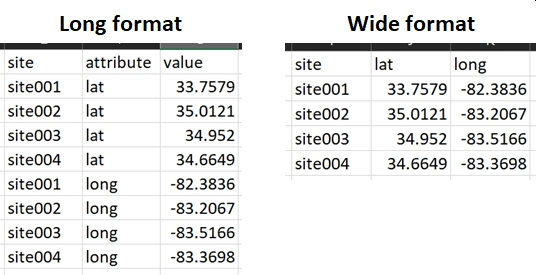
\includegraphics[keepaspectratio]{chapters/../images/05_09.jpg}}

}

\end{figure}%

In a \textbf{long-format dataset}, every \emph{value} is stored in a
separate \emph{row}. The variable (aka: feature or attribute) that each
value represents is kept in a separate \emph{column}. Many public or
online data sources serve datasets in long format. This is usually
because the data are pulled from a database, and it left to the user to
reshape the data to fit their needs. Storing data in this manner can
sometimes be more efficient from a computational standpoint, but it is
usually not convenient for analysis. The reason that long format is
inconvenient for analysis is because all of the information about
individual samples (i.e, observations) are on different rows of the
dataset.

In a \textbf{wide-format dataset}, each row contains \textbf{all values}
associated with a particular \textbf{sample}. This means that each
variable gets its own column, and each cell contains a single value.
This format is sometimes called \textbf{tidy} format by the authors of
the \texttt{tidyverse} set of R packages (Wickham 2014), but researchers
were formatting data this way long before the tidyverse packages or R
were developed (Broman and Woo 2018). As a rule, you should store and
manage your data in wide/tidy format. This format makes it easy to take
advantage of R's vectorized nature. This is also the format expected by
most functions that work with data frames.

Base R has some functions for reshaping data, but most sources recommend
using the \texttt{reshape2} package or the \texttt{tidyverse}. The
examples below demonstrate reshaping a dataset from a typical long
format to a more useful wide format. You will need the file
\href{https://greenquanteco.github.io/reshape_example_2025-08-12.csv}{reshape\_example\_2025-08-12.csv}
in your R home directory and package \texttt{reshape2}.

\begin{Shaded}
\begin{Highlighting}[]
\FunctionTok{library}\NormalTok{(reshape2)}
\NormalTok{in.name }\OtherTok{\textless{}{-}} \StringTok{"reshape\_example\_2025{-}08{-}12.csv"}
\NormalTok{x }\OtherTok{\textless{}{-}} \FunctionTok{read.csv}\NormalTok{(in.name)}
\FunctionTok{head}\NormalTok{(x)}
\DocumentationTok{\#\#       grid attribute      value}
\DocumentationTok{\#\# 1 BART\_062       lat   44.05735}
\DocumentationTok{\#\# 2 BART\_084       lat  44.048501}
\DocumentationTok{\#\# 3 HARV\_001       lat  42.422943}
\DocumentationTok{\#\# 4 HARV\_006       lat  42.401991}
\DocumentationTok{\#\# 5 HARV\_008       lat  42.443394}
\DocumentationTok{\#\# 6 BART\_062       lon {-}71.308646}
\FunctionTok{class}\NormalTok{(x}\SpecialCharTok{$}\NormalTok{value)}
\DocumentationTok{\#\# [1] "character"}
\end{Highlighting}
\end{Shaded}

Notice that the \texttt{value} column contains a mix of numeric and text
values--so the numbers are stored as text. If we wanted to do something
with those values, they need to be pulled out of the vector
\texttt{value} and converted to numeric values. Because a vector can
have only one type of value, the attributes will need to end up in their
own columns. The fastest way to do this is to use the function
\texttt{dcast()} from package \texttt{reshape2}.

\begin{Shaded}
\begin{Highlighting}[]
\NormalTok{dx }\OtherTok{\textless{}{-}} \FunctionTok{dcast}\NormalTok{(x, grid}\SpecialCharTok{\textasciitilde{}}\NormalTok{attribute)}
\NormalTok{dx}\SpecialCharTok{$}\NormalTok{lat }\OtherTok{\textless{}{-}} \FunctionTok{as.numeric}\NormalTok{(dx}\SpecialCharTok{$}\NormalTok{lat)}
\NormalTok{dx}\SpecialCharTok{$}\NormalTok{lon }\OtherTok{\textless{}{-}} \FunctionTok{as.numeric}\NormalTok{(dx}\SpecialCharTok{$}\NormalTok{lon)}
\NormalTok{dx}
\end{Highlighting}
\end{Shaded}

\begin{verbatim}
      grid      lat       lon            nlcd
1 BART_062 44.05735 -71.30865 deciduousForest
2 BART_084 44.04850 -71.29797 evergreenForest
3 HARV_001 42.42294 -72.25872 deciduousForest
4 HARV_006 42.40199 -72.25478 deciduousForest
5 HARV_008 42.44339 -72.22512 deciduousForest
\end{verbatim}

If we needed to go the other way, from wide to long format, we use
function \texttt{melt()}. This is essentially the reverse of
\texttt{dcast()}.

\begin{Shaded}
\begin{Highlighting}[]

\NormalTok{mx }\OtherTok{\textless{}{-}} \FunctionTok{melt}\NormalTok{(dx, }
           \AttributeTok{id.vars=}\StringTok{"grid"}\NormalTok{, }
           \AttributeTok{measure.vars=}\FunctionTok{c}\NormalTok{(}\StringTok{"lat"}\NormalTok{, }\StringTok{"lon"}\NormalTok{, }\StringTok{"nlcd"}\NormalTok{))}

\CommentTok{\# default:}
\FunctionTok{head}\NormalTok{(mx)}
\DocumentationTok{\#\#       grid variable      value}
\DocumentationTok{\#\# 1 BART\_062      lat   44.05735}
\DocumentationTok{\#\# 2 BART\_084      lat  44.048501}
\DocumentationTok{\#\# 3 HARV\_001      lat  42.422943}
\DocumentationTok{\#\# 4 HARV\_006      lat  42.401991}
\DocumentationTok{\#\# 5 HARV\_008      lat  42.443394}
\DocumentationTok{\#\# 6 BART\_062      lon {-}71.308646}

\CommentTok{\# sort by grid, then variable:}
\FunctionTok{head}\NormalTok{(mx[}\FunctionTok{order}\NormalTok{(mx}\SpecialCharTok{$}\NormalTok{grid, mx}\SpecialCharTok{$}\NormalTok{variable),])}
\DocumentationTok{\#\#        grid variable           value}
\DocumentationTok{\#\# 1  BART\_062      lat        44.05735}
\DocumentationTok{\#\# 6  BART\_062      lon      {-}71.308646}
\DocumentationTok{\#\# 11 BART\_062     nlcd deciduousForest}
\DocumentationTok{\#\# 2  BART\_084      lat       44.048501}
\DocumentationTok{\#\# 7  BART\_084      lon      {-}71.297965}
\DocumentationTok{\#\# 12 BART\_084     nlcd evergreenForest}
\end{Highlighting}
\end{Shaded}

The \texttt{tidyverse} equivalents for \texttt{melt()} and
\texttt{dcast()} are \texttt{pivot\_longer()} and
\texttt{pivot\_wider()}, respectively. The syntax of these
\texttt{tidyverse} functions are similar to the \texttt{reshape2}
functions. Note that the \texttt{tidyverse} functions will output a
\textbf{tibble}, which is a form of data frame peculiar to the
\texttt{tidyverse}. Some non-\texttt{tidyverse} functions can use
tibbles, and some cannot. Tibbles can be converted to base R data frames
with function \texttt{data.frame()}.

\begin{Shaded}
\begin{Highlighting}[]

\FunctionTok{library}\NormalTok{(tidyr)}

\CommentTok{\# long to wide:}
\CommentTok{\# eqv. to reshape2::dcast}
\NormalTok{tdx }\OtherTok{\textless{}{-}} \FunctionTok{pivot\_wider}\NormalTok{(x, }
                   \AttributeTok{names\_from=}\StringTok{"attribute"}\NormalTok{,}
                   \AttributeTok{values\_from=}\StringTok{"value"}\NormalTok{)}
\FunctionTok{head}\NormalTok{(tdx)}
\DocumentationTok{\#\# \# A tibble: 5 x 4}
\DocumentationTok{\#\#   grid     lat       lon        nlcd           }
\DocumentationTok{\#\#   \textless{}chr\textgreater{}    \textless{}chr\textgreater{}     \textless{}chr\textgreater{}      \textless{}chr\textgreater{}          }
\DocumentationTok{\#\# 1 BART\_062 44.05735  {-}71.308646 deciduousForest}
\DocumentationTok{\#\# 2 BART\_084 44.048501 {-}71.297965 evergreenForest}
\DocumentationTok{\#\# 3 HARV\_001 42.422943 {-}72.258721 deciduousForest}
\DocumentationTok{\#\# 4 HARV\_006 42.401991 {-}72.254785 deciduousForest}
\DocumentationTok{\#\# 5 HARV\_008 42.443394 {-}72.225117 deciduousForest}

\CommentTok{\# wide to long:}
\CommentTok{\# eqv. to reshape2::melt}
\NormalTok{tmx }\OtherTok{\textless{}{-}} \FunctionTok{pivot\_longer}\NormalTok{(tdx,}
               \AttributeTok{cols=}\FunctionTok{c}\NormalTok{(}\StringTok{"lat"}\NormalTok{, }\StringTok{"lon"}\NormalTok{, }\StringTok{"nlcd"}\NormalTok{),}
               \AttributeTok{names\_to=}\StringTok{"variable"}\NormalTok{)}
\FunctionTok{head}\NormalTok{(tmx)}
\DocumentationTok{\#\# \# A tibble: 6 x 3}
\DocumentationTok{\#\#   grid     variable value          }
\DocumentationTok{\#\#   \textless{}chr\textgreater{}    \textless{}chr\textgreater{}    \textless{}chr\textgreater{}          }
\DocumentationTok{\#\# 1 BART\_062 lat      44.05735       }
\DocumentationTok{\#\# 2 BART\_062 lon      {-}71.308646     }
\DocumentationTok{\#\# 3 BART\_062 nlcd     deciduousForest}
\DocumentationTok{\#\# 4 BART\_084 lat      44.048501      }
\DocumentationTok{\#\# 5 BART\_084 lon      {-}71.297965     }
\DocumentationTok{\#\# 6 BART\_084 nlcd     evergreenForest}

\CommentTok{\# if needed:}
\NormalTok{tdx.df }\OtherTok{\textless{}{-}} \FunctionTok{data.frame}\NormalTok{(tdx)}
\end{Highlighting}
\end{Shaded}

\part{Exploratory data analysis with R}

Blah blah test test test.

\chapter{Basic descriptive statistics}\label{sec-desc}

One of the first steps in exploratory data analysis is understanding how
values in a variable are spread out (aka: distributed), and what a
``typical'' value is.

Biologists use a few common \textbf{summary statistics}, or
\textbf{descriptive statistics}, to describe variables. What makes
descriptive statistics is that they are calculated directly from the
data, and do not estimate any unknown parameters. Estimating unknown
parameters is the realm of \textbf{inferential statistics}. Any method
that tests a hypothesis--such as a \emph{t}-test, ANOVA, linear
regression, etc.--is an inferential technique.

\section{Sample and population statistics}\label{sec-desc-sp}

In biology, we never have all of the possible values which could be
observed. For example, if you wanted to study the body masses of
squirrels, you could go and collect, say, 30 squirrels and weigh them.
However, those 30 are only a small fraction of the millions of squirrels
alive in the world. You would be assuming that your 30 squirrels somehow
represent all squirrels.

\begin{itemize}
\item
  The values that are observed are \textbf{samples}, and they are
  summarized by \textbf{sample statistics}.
\item
  The set of all possible values that could be observed, even if only in
  principle, are the \textbf{population}. \textbf{Population parameters}
  or \textbf{population statistics} describe this set of all possible
  values.
\end{itemize}

In science, we usually want to \emph{estimate} population parameters,
but these are unobservable. Instead, we use sample statistics to
estimate the parameters of the underlying population.

\begin{figure}[H]

\caption{Illustration of how sampling bias can affect estimates of
population parameters like the sample mean \(\bar{x}\) and sample
standard deviation \(s\).}

{\centering \pandocbounded{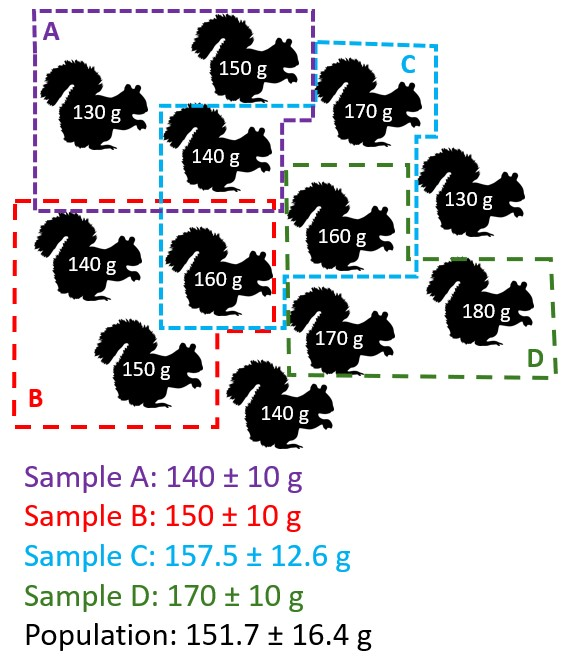
\includegraphics[keepaspectratio]{chapters/../images/06_01.jpg}}

}

\end{figure}%

In the figure above, the \emph{population mean} of all squirrels is
151.7 g. However, finding all squirrels in an area (much less the world)
is not practical. So, researchers took 4 samples of a few squirrels
each, and obtained \emph{sample means} of 140, 150, 157.5, and 170 g.
Notice that the mean of these sample means, 154.38 g, is pretty close to
the population mean. In fact, the more squirrels you include in your
sample, the less uncertain your estimate of the mean will be. In the
figure below, notice that as the size of the sample increases, the range
of estimates of the mean shrinks.

\begin{Shaded}
\begin{Highlighting}[]
\NormalTok{all.wts }\OtherTok{\textless{}{-}} \FunctionTok{c}\NormalTok{(}\DecValTok{130}\NormalTok{, }\DecValTok{150}\NormalTok{, }\DecValTok{170}\NormalTok{,}
             \DecValTok{140}\NormalTok{, }\DecValTok{140}\NormalTok{, }\DecValTok{160}\NormalTok{,}
             \DecValTok{160}\NormalTok{, }\DecValTok{130}\NormalTok{, }\DecValTok{150}\NormalTok{,}
             \DecValTok{170}\NormalTok{, }\DecValTok{180}\NormalTok{, }\DecValTok{140}\NormalTok{)}
\NormalTok{npop }\OtherTok{\textless{}{-}} \FunctionTok{length}\NormalTok{(all.wts)}
\NormalTok{ns }\OtherTok{\textless{}{-}} \DecValTok{2}\SpecialCharTok{:}\NormalTok{npop}
\NormalTok{ests }\OtherTok{\textless{}{-}} \FunctionTok{vector}\NormalTok{(}\StringTok{"list"}\NormalTok{, }\FunctionTok{length}\NormalTok{(ns))}
\ControlFlowTok{for}\NormalTok{(i }\ControlFlowTok{in} \DecValTok{1}\SpecialCharTok{:}\FunctionTok{length}\NormalTok{(ns))\{}
\NormalTok{  ests[[i]] }\OtherTok{\textless{}{-}} \FunctionTok{combn}\NormalTok{(all.wts, }\AttributeTok{m=}\NormalTok{ns[i], }\AttributeTok{FUN=}\NormalTok{mean)}
\NormalTok{\}}

\NormalTok{mins }\OtherTok{\textless{}{-}} \FunctionTok{sapply}\NormalTok{(ests, min)}
\NormalTok{maxs }\OtherTok{\textless{}{-}} \FunctionTok{sapply}\NormalTok{(ests, max)}
\NormalTok{meds }\OtherTok{\textless{}{-}} \FunctionTok{sapply}\NormalTok{(ests, median)}
\FunctionTok{plot}\NormalTok{(ns, meds, }\AttributeTok{type=}\StringTok{"o"}\NormalTok{, }\AttributeTok{pch=}\DecValTok{16}\NormalTok{,}
  \AttributeTok{ylim=}\FunctionTok{c}\NormalTok{(}\DecValTok{120}\NormalTok{, }\DecValTok{180}\NormalTok{), }\AttributeTok{cex=}\DecValTok{2}\NormalTok{, }\AttributeTok{lwd=}\DecValTok{4}\NormalTok{,}
  \AttributeTok{ylab=}\StringTok{"Estimate of mean"}\NormalTok{, }\AttributeTok{xlab=}\StringTok{"Size of sample"}\NormalTok{)}
\FunctionTok{segments}\NormalTok{(ns, mins, ns, maxs, }\AttributeTok{lwd=}\DecValTok{2}\NormalTok{)}
\end{Highlighting}
\end{Shaded}

\pandocbounded{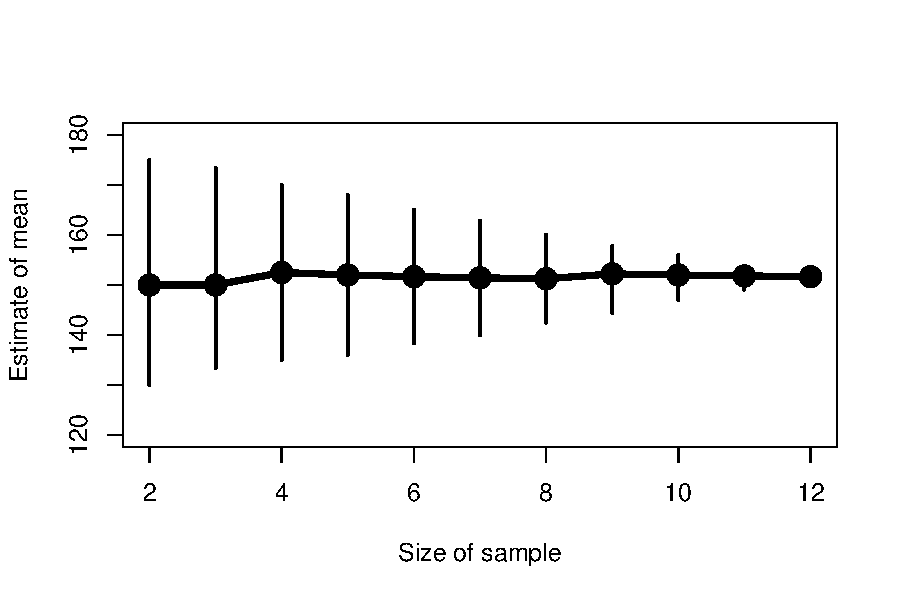
\includegraphics[keepaspectratio]{chapters/ch06_files/figure-pdf/unnamed-chunk-1-1.pdf}}

\section{Central tendency}\label{sec-desc-cen}

The \textbf{central tendency} of a variable is a value that represents a
``typical'' value from that set of values. Central tendency is usually
expressed in one of three ways:

\begin{itemize}
\item
  \textbf{Mean}: the sum of values divided by the number of values. This
  value is also called the ``\textbf{arithmetic mean}''. Answers the
  question, ``\emph{What value would all values be if they were the
  same}?''. When people say ``mean'' or ``average'', this usually what
  they are referring to. The mean is useful because it is one of the
  defining features of the \textbf{normal distribution}, a foundational
  concept in modern statistics.
\item
  \textbf{Median}: the middle value, which is greater than half of the
  values and less than the other half of the values. Also known as the
  50\textsuperscript{th} percentile or 0.5 quantile. Answer the
  question, ``\emph{If you lined up the values from smallest to largest,
  what value would be in the middle?}''.
\item
  \textbf{Mode}: the most common value.
\end{itemize}

For many datasets, the mean and median will be approximately the same.
Data that are \textbf{skewed} will have a median different from their
mean.

\begin{figure}[H]

\caption{Illustration of \emph{skew}. The solid black line shows an
unskewed distribution that is roughly symmetrical about its mean, with
its mean and median almost identical. The dashed red line shows a
right-skewed distribution that has mostly small values and very few
large values. Its median is very different from its mean.}

{\centering \pandocbounded{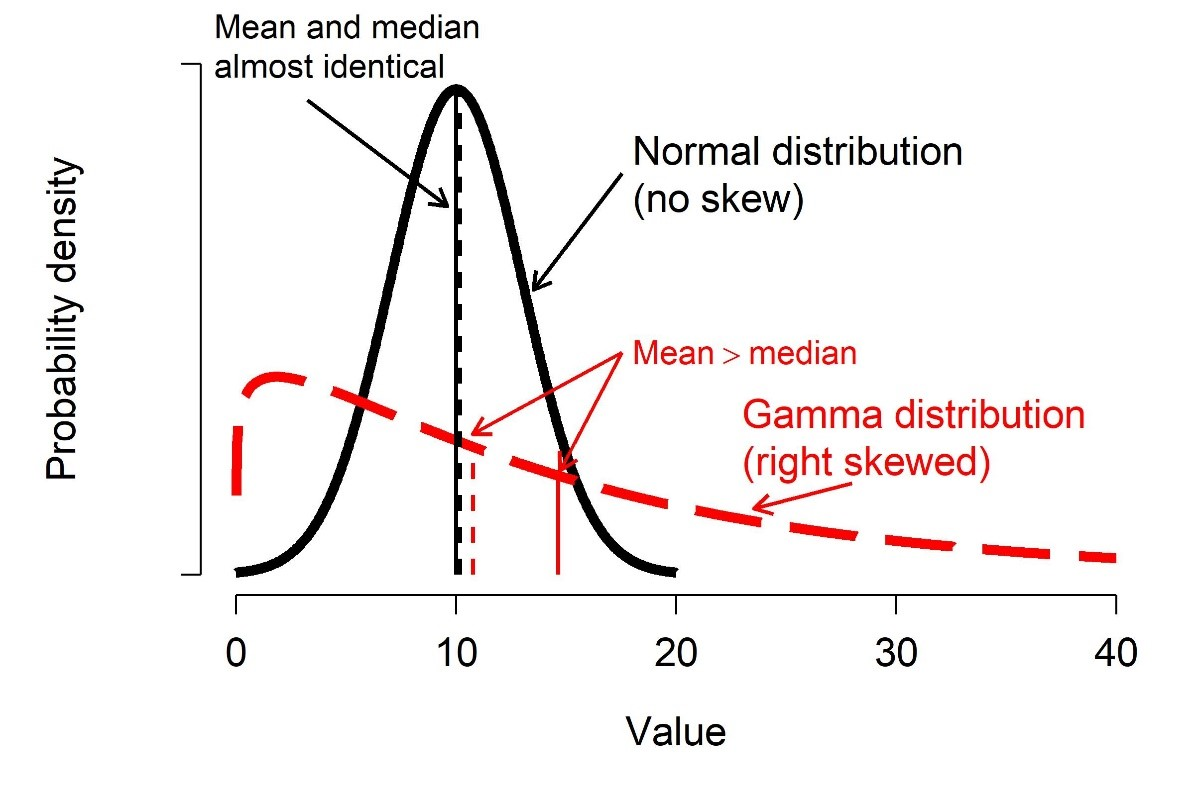
\includegraphics[keepaspectratio]{chapters/../images/06_02.jpg}}

}

\end{figure}%

Biologists typically summarize data using the mean, but median can be
appropriate in some situations--especially when data are not normally
distributed.

\subsection{Means}\label{sec-desc-cen-mean}

\subsubsection{Arithmetic mean}\label{sec-desc-cen-mean-am}

The \textbf{arithmetic mean} or just \textbf{mean} is the value that all
values would be if they were all the same. Biologists consider both the
\textbf{sample mean} \(\bar{x}\) and the \textbf{population mean}
\(\mu\).

\begin{itemize}
\item
  The \textbf{population mean} \(\mu\) is the mean of all possible
  observations, and defines the underlying distribution of values. This
  can be a parameter of a distribution, but is usually unknown in
  practice and has to be estimated from data.
\item
  The \textbf{sample mean} is \(\bar{x}\) the mean of observed values.
\end{itemize}

The sample mean is calculated as the sum of all values in \emph{x}
divided by the number of values \emph{n}:

\[\bar{x}=\frac{\sum_{i=1}^{n}x_i}{n}\]

The mean is useful because it is part of the definition of the normal
distribution, a very important concept in modern statistics.

You can get the mean of a variable in R using the function
\texttt{mean()}:

\begin{Shaded}
\begin{Highlighting}[]
\CommentTok{\# random normal dist. with mean = 5 and sd = 1}
\NormalTok{x }\OtherTok{\textless{}{-}} \FunctionTok{rnorm}\NormalTok{(}\DecValTok{100}\NormalTok{, }\DecValTok{5}\NormalTok{, }\DecValTok{1}\NormalTok{)}
\FunctionTok{mean}\NormalTok{(x)}
\end{Highlighting}
\end{Shaded}

\begin{verbatim}
[1] 4.986525
\end{verbatim}

Like many summarization functions in R, \texttt{mean()} does not
automatically handle missing values (\texttt{NA}). If your dataset
contains missing values, you need to set the argument
\texttt{na.rm=TRUE}. This can seem like an annoying bug, but it's
actually a feature. By returning \texttt{NA} when the data contain
missing values, R is helping you track down where missing values are
coming from (and thus, why your code may not be working at some later
point).

\begin{Shaded}
\begin{Highlighting}[]

\NormalTok{x }\OtherTok{\textless{}{-}} \FunctionTok{c}\NormalTok{(}\DecValTok{2}\NormalTok{, }\DecValTok{3}\NormalTok{, }\DecValTok{6}\NormalTok{, }\DecValTok{2}\NormalTok{, }\DecValTok{6}\NormalTok{, }\DecValTok{1}\NormalTok{, }\ConstantTok{NA}\NormalTok{)}
\FunctionTok{mean}\NormalTok{(x)}
\DocumentationTok{\#\# [1] NA}
\FunctionTok{mean}\NormalTok{(x, }\AttributeTok{na.rm=}\ConstantTok{TRUE}\NormalTok{)}
\DocumentationTok{\#\# [1] 3.333333}
\end{Highlighting}
\end{Shaded}

While most poeple only ever use the arithmetic mean, there are other
means.

\subsubsection{Geometric mean}\label{sec-desc-cen-mean-gm}

The \textbf{geometric mean} is defined as the \emph{n}-th root of the
product of all values:

\[GM\left(x\right)=\sqrt[n]{\prod_{i=1}^{n}x}\]

Or equivalently, as Euler's constant \emph{e} raised to the power of the
mean of the values on the log scale\footnote{Natural log. Unless
  otherwise indicated, always assume a mathematician or statistician
  means natural log.}:

\[GM\left(x\right)=exp\left(\frac{1}{n}\sum_{i=1}^{n}\log{\left(x\right)}\right)\]

The geometric mean is sometimes used for values that are meant to be
multiplied together, such as growth rates. One application is in
comparative morphology, where the geometric mean of a set of anatomical
measurements is used as a sort of overall measure of body size against
which individual measurements can be relativized. For example, a
morphologist might calculate the geometric mean of 15 skull measurements
to arrive at the size of a ``hypervolume'' which represents skull size.

Because of the way that it is defined, the geometric mean is only
defined for positive real values.

There is no base function for geometric mean, but it's easy to get by
combining base functions.

\begin{Shaded}
\begin{Highlighting}[]

\CommentTok{\# lognormal with logmean 2 and logsd=0.5}
\NormalTok{x }\OtherTok{\textless{}{-}} \FunctionTok{rlnorm}\NormalTok{(}\DecValTok{10}\NormalTok{, }\DecValTok{2}\NormalTok{, }\FloatTok{0.5}\NormalTok{)}

\CommentTok{\# custom function for geometric mean:}
\NormalTok{geomean }\OtherTok{\textless{}{-}} \ControlFlowTok{function}\NormalTok{(x)\{}\FunctionTok{exp}\NormalTok{(}\FunctionTok{mean}\NormalTok{(}\FunctionTok{log}\NormalTok{(x)))\}}

\CommentTok{\# test it out:}
\FunctionTok{geomean}\NormalTok{(x)}
\DocumentationTok{\#\# [1] 6.048237}

\CommentTok{\# another way:}
\NormalTok{geomean2 }\OtherTok{\textless{}{-}} \ControlFlowTok{function}\NormalTok{(x)\{}\FunctionTok{prod}\NormalTok{(x)}\SpecialCharTok{\^{}}\NormalTok{(}\DecValTok{1}\SpecialCharTok{/}\FunctionTok{length}\NormalTok{(x))\}}
\FunctionTok{geomean2}\NormalTok{(x)}
\DocumentationTok{\#\# [1] 6.048237}
\end{Highlighting}
\end{Shaded}

\subsubsection{Harmonic mean}\label{sec-desc-cen-mean-hm}

The \textbf{harmonic mean} is less common than the arithmetic or
geometric means. It is used when an average \emph{rate} is needed. The
harmonic mean is the reciprocal of the arithmetic mean of reciprocals of
the values:

\[HM\left(x\right)=\left(\frac{1}{n}\sum_{i=1}^{n}x^{-1}\right)^{-1}\]

An example use case for the harmonic mean is as follows: a migrating
bird travels from Atlanta to Knoxville, Tennessee (250 km) at an average
speed of 60 km/h, and then from Knoxville to Lexington, Kentucky (230
km) at an average speed of 52 km/h. Its average speed on the trip is not
the arithmetic mean of the speeds, but the harmonic mean:

\[HM\left(v\right)=\frac{Total\ distance}{Total\ time}=\frac{2}{\frac{1}{60}+\frac{1}{52}}\approx55.7\ km/h\]

I'm not aware of a base function for harmonic means, but it is easy to
get:

\begin{Shaded}
\begin{Highlighting}[]

\CommentTok{\# only defined for postive real values}
\NormalTok{a }\OtherTok{\textless{}{-}} \FunctionTok{rlnorm}\NormalTok{(}\DecValTok{20}\NormalTok{, }\DecValTok{3}\NormalTok{, }\DecValTok{1}\NormalTok{)}

\CommentTok{\# custom function to get harmonic mean}
\NormalTok{har.mean }\OtherTok{\textless{}{-}} \ControlFlowTok{function}\NormalTok{(x)\{}\DecValTok{1}\SpecialCharTok{/}\NormalTok{(}\FunctionTok{mean}\NormalTok{(}\DecValTok{1}\SpecialCharTok{/}\NormalTok{x))\}}

\CommentTok{\# compare mean, geometric mean, and harmonic mean:}
\FunctionTok{mean}\NormalTok{(a)}
\DocumentationTok{\#\# [1] 38.8423}
\FunctionTok{geomean}\NormalTok{(a)}
\DocumentationTok{\#\# [1] 26.54886}
\FunctionTok{har.mean}\NormalTok{(a)}
\DocumentationTok{\#\# [1] 17.04769}
\end{Highlighting}
\end{Shaded}

Interestingly, for any set of positive values with at least 2 unique
values, the following inequality will always be true:

\[AM\left(x\right)>GM\left(x\right)>HM\left(x\right)\]

\subsubsection{Weighted mean}\label{sec-desc-cen-mean-wm}

Sometimes we need to some observations to count more than others. The
\textbf{weight} of an observation is the amount that it contributes to a
statistic or analysis. A \textbf{weighted mean} is useful when some
observations represent more data or experimental units.

For example, when trying to calculate the mean mass of elephants across
multiple populations, it might make sense to calculate the mean of the
population-level means, but weight the population means by the number of
elephants measured in each population. This would be done because the
populations with more measurements represent more data, and thus give us
greater confidence about what the true mean might be.

The R function for the weighted mean takes a set of values \texttt{x}
and weights \texttt{w}. The weights in \texttt{w} must add up to 1.

\begin{Shaded}
\begin{Highlighting}[]

\CommentTok{\# make some values}
\NormalTok{x }\OtherTok{\textless{}{-}} \FunctionTok{c}\NormalTok{(}\DecValTok{14}\NormalTok{, }\DecValTok{3}\NormalTok{, }\DecValTok{5}\NormalTok{, }\DecValTok{4}\NormalTok{)}

\CommentTok{\# weights}
\CommentTok{\# defining as fractions over total}
\CommentTok{\# sample size will guarantee sum(wts)==1}
\NormalTok{wts }\OtherTok{\textless{}{-}} \FunctionTok{c}\NormalTok{(}\DecValTok{10}\NormalTok{, }\DecValTok{1}\NormalTok{, }\DecValTok{1}\NormalTok{, }\DecValTok{2}\NormalTok{)}\SpecialCharTok{/}\DecValTok{14}

\CommentTok{\# compare mean to weighted mean}
\FunctionTok{mean}\NormalTok{(x)}
\DocumentationTok{\#\# [1] 6.5}
\FunctionTok{weighted.mean}\NormalTok{(x, wts)}
\DocumentationTok{\#\# [1] 11.14286}
\end{Highlighting}
\end{Shaded}

\subsection{Median}\label{sec-desc-cen-med}

The \textbf{median} is the central value of a set of values. If you were
to rank the values from smallest to largest, the median would be the
value in the middle (or, if there were an even number of values, the
median would be the mean of the two central values). The median is also
known as the 50\textsuperscript{th} percentile, or 0.5 quantile.

The median is sometimes a more useful measure of central tendency than
the mean when data are strongly skewed. A classic use case is personal
income. In 2020, the US median household income was about \$67000. It's
hard to find exact numbers, but at one point in 2020 Jeff Bezos had made
about \$13 billion since 2019. This implies that in a room with 99
``average'' Americans and 1 Jeff Bezos, the \emph{mean} annual income
was about \$130 million. Is that a good representation of what most
households made?

Of course not. However, the median would be about \$67000, which would
be more representative.

The easiest way to get the median in R is with the \texttt{median()}
function. You can also use \texttt{quantile()} with argument
\texttt{probs} (the second argument) set to 0.5.

\begin{Shaded}
\begin{Highlighting}[]
\NormalTok{x }\OtherTok{\textless{}{-}} \FunctionTok{rnorm}\NormalTok{(}\DecValTok{100}\NormalTok{)}
\FunctionTok{median}\NormalTok{(x)}
\DocumentationTok{\#\# [1] {-}0.2467164}
\FunctionTok{quantile}\NormalTok{(x, }\FloatTok{0.5}\NormalTok{)}
\DocumentationTok{\#\#        50\% }
\DocumentationTok{\#\# {-}0.2467164}
\end{Highlighting}
\end{Shaded}

\subsection{Mode}\label{sec-desc-cen-mode}

The \textbf{mode} is the \emph{most common value} in a set of values.
For many distributions, the mode will be the same as, or close to, the
mean and median. Most distributions have one mode, or are
\textbf{unimodal}. Another common case is distributions with two modes,
or are \textbf{bimodal}.

There is no base function to get the mode, but it can be obtained in
several ways by combining base functions.

\begin{Shaded}
\begin{Highlighting}[]

\CommentTok{\# generate some random values in 1:8}
\FunctionTok{set.seed}\NormalTok{(}\DecValTok{123}\NormalTok{)}
\NormalTok{a }\OtherTok{\textless{}{-}} \FunctionTok{sample}\NormalTok{(}\DecValTok{1}\SpecialCharTok{:}\DecValTok{8}\NormalTok{, }\DecValTok{20}\NormalTok{, }\AttributeTok{replace=}\ConstantTok{TRUE}\NormalTok{)}

\CommentTok{\# simple function for mode}
\CommentTok{\# Will return \textgreater{}1 result if \textgreater{}1 mode.}
\CommentTok{\# Capitalized because already a function called "mode" that}
\CommentTok{\# does something else and don\textquotesingle{}t want to overwrite it}
\NormalTok{Mode }\OtherTok{\textless{}{-}} \ControlFlowTok{function}\NormalTok{(x)\{}
\NormalTok{    un }\OtherTok{\textless{}{-}} \FunctionTok{sort}\NormalTok{(}\FunctionTok{unique}\NormalTok{(x))}
\NormalTok{    ta }\OtherTok{\textless{}{-}} \FunctionTok{table}\NormalTok{(x)}
\NormalTok{    mx }\OtherTok{\textless{}{-}} \FunctionTok{max}\NormalTok{(ta)}
    \FunctionTok{return}\NormalTok{(un[}\FunctionTok{which}\NormalTok{(ta}\SpecialCharTok{==}\NormalTok{mx)])}
\NormalTok{\}}
\FunctionTok{Mode}\NormalTok{(a)}
\DocumentationTok{\#\# [1] 3}

\CommentTok{\# illustration with 2 modes:}
\NormalTok{b }\OtherTok{\textless{}{-}} \FunctionTok{c}\NormalTok{(}\DecValTok{4}\NormalTok{,}\DecValTok{4}\NormalTok{,}\DecValTok{4}\NormalTok{,}\DecValTok{3}\NormalTok{,}\DecValTok{3}\NormalTok{,}\DecValTok{3}\NormalTok{,}\DecValTok{2}\NormalTok{,}\DecValTok{1}\NormalTok{)}
\FunctionTok{Mode}\NormalTok{(b)}
\DocumentationTok{\#\# [1] 3 4}
\end{Highlighting}
\end{Shaded}

Another way to get the mode is to find peaks on a kernel density plot.
We'll discuss what these plots really mean later in
Section~\ref{sec-plot1-sing-kern}, but for now, a kernel density plot
shows how likely different values are a distribution. This method might
be more useful when there are many values, or the values have a great
deal of precision, making it hard to find a mode by counting up
occurrences.

In the example below, the distribution has a peak around \(x=12.01\).
This means that the mode is about 12.01, which is very close to the mean
and median as well as the true mean used to generate the distribution.

\begin{Shaded}
\begin{Highlighting}[]
\FunctionTok{set.seed}\NormalTok{(}\DecValTok{123}\NormalTok{)}
\NormalTok{a }\OtherTok{\textless{}{-}} \FunctionTok{rnorm}\NormalTok{(}\FloatTok{1e3}\NormalTok{, }\DecValTok{12}\NormalTok{, }\DecValTok{2}\NormalTok{)}
\NormalTok{den }\OtherTok{\textless{}{-}} \FunctionTok{density}\NormalTok{(a)}
\FunctionTok{plot}\NormalTok{(den)}
\FunctionTok{points}\NormalTok{(den}\SpecialCharTok{$}\NormalTok{x[}\FunctionTok{which.max}\NormalTok{(den}\SpecialCharTok{$}\NormalTok{y)], }\FunctionTok{max}\NormalTok{(den}\SpecialCharTok{$}\NormalTok{y),}
    \AttributeTok{pch=}\DecValTok{16}\NormalTok{, }\AttributeTok{col=}\StringTok{"red"}\NormalTok{, }\AttributeTok{cex=}\DecValTok{2}\NormalTok{)}
\end{Highlighting}
\end{Shaded}

\pandocbounded{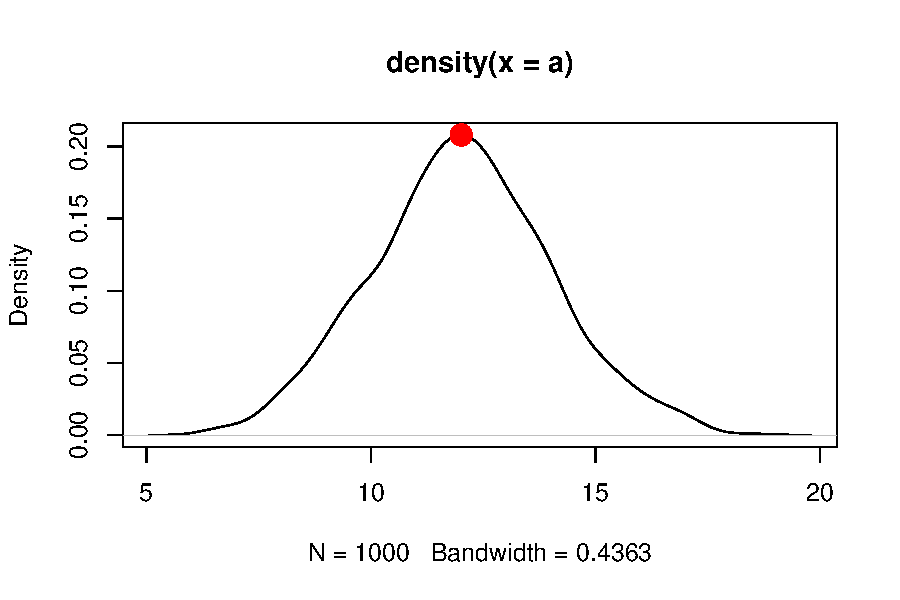
\includegraphics[keepaspectratio]{chapters/ch06_files/figure-pdf/unnamed-chunk-9-1.pdf}}

\begin{Shaded}
\begin{Highlighting}[]
\CommentTok{\# function to estimate mode}
\NormalTok{Mode2 }\OtherTok{\textless{}{-}} \ControlFlowTok{function}\NormalTok{(x)\{}
\NormalTok{    de }\OtherTok{\textless{}{-}} \FunctionTok{density}\NormalTok{(x)}
    \FunctionTok{return}\NormalTok{(de}\SpecialCharTok{$}\NormalTok{x[}\FunctionTok{which.max}\NormalTok{(de}\SpecialCharTok{$}\NormalTok{y)])}
\NormalTok{\}}
\FunctionTok{Mode2}\NormalTok{(a)}
\end{Highlighting}
\end{Shaded}

\begin{verbatim}
[1] 12.0136
\end{verbatim}

The function we made, \texttt{Mode2()}, works well enough if there is
only one mode.

But, many real life distributions have \(>1\) mode. Such distributions
are called \textbf{bimodal} if they have 2 modes, or \textbf{multimodal}
if they have 3 or more. A classic example of bimodality is grades in
college courses: it is very common to have many Bs, and many Ds, but not
many Fs, Cs, or As.

If your data appear to have \(>1\) mode, you can estimate them by
finding points where the slope of the density plot changes sign. The
code below is inelegant but it works.

\begin{Shaded}
\begin{Highlighting}[]
\FunctionTok{set.seed}\NormalTok{(}\DecValTok{123}\NormalTok{)}
\NormalTok{a1 }\OtherTok{\textless{}{-}} \FunctionTok{rnorm}\NormalTok{(}\FloatTok{1e2}\NormalTok{, }\DecValTok{12}\NormalTok{, }\DecValTok{2}\NormalTok{)}
\NormalTok{a2 }\OtherTok{\textless{}{-}} \FunctionTok{rnorm}\NormalTok{(}\FloatTok{1e2}\NormalTok{, }\DecValTok{20}\NormalTok{, }\DecValTok{2}\NormalTok{)}
\NormalTok{a }\OtherTok{\textless{}{-}} \FunctionTok{c}\NormalTok{(a1, a2)}
\NormalTok{den }\OtherTok{\textless{}{-}} \FunctionTok{density}\NormalTok{(a)}

\CommentTok{\# shows bimodal distribution:}
\FunctionTok{plot}\NormalTok{(den)}

\CommentTok{\# function to find peaks on density plot}
\CommentTok{\# i.e., where slope changes from positive to negative}
\NormalTok{Mode3 }\OtherTok{\textless{}{-}} \ControlFlowTok{function}\NormalTok{(x)\{}
\NormalTok{    de }\OtherTok{\textless{}{-}} \FunctionTok{density}\NormalTok{(x)}
\NormalTok{    dif }\OtherTok{\textless{}{-}} \FunctionTok{diff}\NormalTok{(de}\SpecialCharTok{$}\NormalTok{y)}
\NormalTok{    flag }\OtherTok{\textless{}{-}} \FunctionTok{numeric}\NormalTok{(}\FunctionTok{length}\NormalTok{(dif))}
    \ControlFlowTok{for}\NormalTok{(i }\ControlFlowTok{in} \DecValTok{2}\SpecialCharTok{:}\FunctionTok{length}\NormalTok{(dif))\{}
        \ControlFlowTok{if}\NormalTok{(dif[i}\DecValTok{{-}1}\NormalTok{] }\SpecialCharTok{\textgreater{}=} \DecValTok{0} \SpecialCharTok{\&}\NormalTok{ dif[i] }\SpecialCharTok{\textless{}} \DecValTok{0}\NormalTok{)\{flag[i] }\OtherTok{\textless{}{-}} \DecValTok{1}\NormalTok{\}}
\NormalTok{    \}}\CommentTok{\#i    }
    \FunctionTok{return}\NormalTok{(de}\SpecialCharTok{$}\NormalTok{x[}\FunctionTok{which}\NormalTok{(flag}\SpecialCharTok{==}\DecValTok{1}\NormalTok{)])}
\NormalTok{\}}
\FunctionTok{Mode3}\NormalTok{(a)}
\end{Highlighting}
\end{Shaded}

\begin{verbatim}
[1] 12.03519 19.55226
\end{verbatim}

\begin{Shaded}
\begin{Highlighting}[]
\FunctionTok{abline}\NormalTok{(}\AttributeTok{v=}\FunctionTok{Mode3}\NormalTok{(a), }\AttributeTok{lwd=}\DecValTok{2}\NormalTok{, }\AttributeTok{col=}\StringTok{"red"}\NormalTok{)}
\end{Highlighting}
\end{Shaded}

\pandocbounded{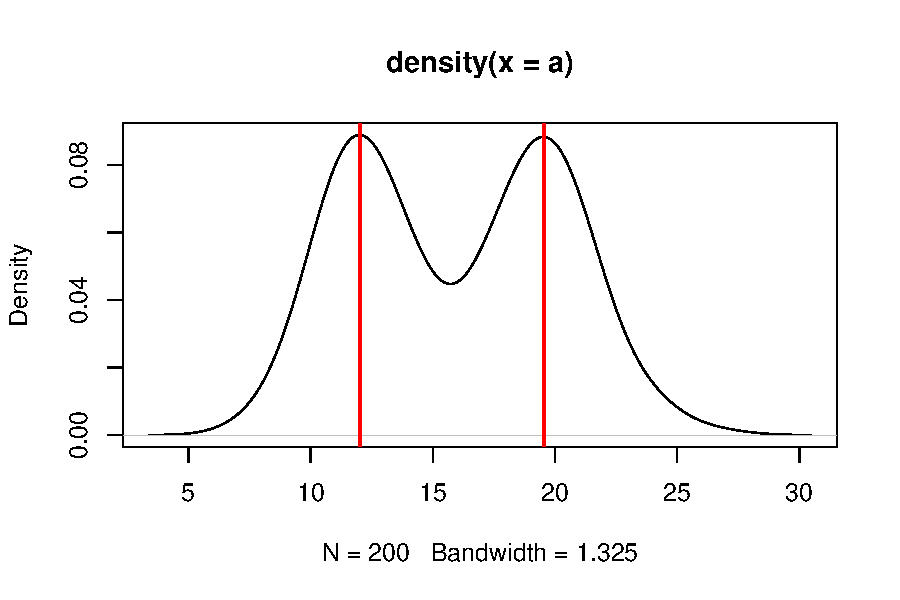
\includegraphics[keepaspectratio]{chapters/ch06_files/figure-pdf/unnamed-chunk-10-1.pdf}}

\section{Variability}\label{sec-desc-var}

\subsection{Variance and standard deviation
(SD)}\label{sec-desc-var-var}

Variability, both random and otherwise, is the \emph{sine qua non} of
statistics. If it weren't for all the uncertainty and variability
inherent in experimental and real world data, data analysis would be a
lot easier and we would barely \href{https://xkcd.com/793/}{need a whole
field for it}. Understanding variability starts with summarizing it.

The classical way to express the variability in a dataset is the
\textbf{variance}. Just like with the mean, we use different symbols for
different variances:

\begin{itemize}
\item
  The \textbf{population variance} \(\sigma^2\) (``sigma squared'')
  defines the normal distribution, and describes the spread of all
  possible observations.
\item
  The \textbf{sample variance} \(s^2\) (``s squared'') is the variance
  of a set of observations (i.e., a sample).
\end{itemize}

The variance is defined as the expected (mean) squared deviation from
the mean:

\[\sigma^2\left(x\right)=\frac{1}{n}\sum_{i=1}^{n}\left(x_i-\mu\right)^2\]

The sample variance of a set of observations is calculated the same way,
except the sample mean \(\bar{x}\) replaces the population mean \(\mu\)
in the expression.

Like the mean \(\mu\), the variance \(\sigma^2\) is part of the
definition of the normal distribution and so it shows up a lot in
statistics.

The differences between each value \(x_i\) and the mean are squared for
two reasons: first, so that positive and negative deviations do not
cancel out (because the square of any real number is positive); and
second, so that greater deviations count more than small deviations.

The main drawback of the variance is that it is in \emph{squared} units
of the original values. For example, the variance of a set of length
measurements taken in cm will be in units of cm\textsuperscript{2}.
Trying to think about lengths in units of area is kind of silly.

For this reason, the variance is often expressed as its square root, the
\textbf{standard deviation (SD)}. As with the variance and mean, we use
different symbols to distinguish between the \textbf{population SD}
\(\sigma\) (``sigma'') and the \textbf{sample SD} \(s\).

The population SD is defined as:

\[\sigma\left(x\right)=\sqrt{\sigma^2\left(x\right)}\]

The expression for the sample SD is the same, except that the sample
variance \(s^2\) replaces the population variance \(\sigma^2\). Because
the SD is the square root of the variance, it is in the same units as
the original measurements (and thus, the mean). This makes SD easier to
interpret than the variance.

For even more convenience, the \textbf{coefficient of variation (CV)} is
the ratio of the SD to the mean. Some people prefer CV to SD because it
allows comparisons between variables with very different means or SD. CV
can be expressed as ratios or as percentages. Whichever you use, just be
clear about what you did.

\begin{Shaded}
\begin{Highlighting}[]

\FunctionTok{set.seed}\NormalTok{(}\DecValTok{123}\NormalTok{)}
\CommentTok{\# different SD, same CV:}
\NormalTok{a }\OtherTok{\textless{}{-}} \FunctionTok{rnorm}\NormalTok{(}\DecValTok{1000}\NormalTok{, }\DecValTok{4}\NormalTok{, }\DecValTok{2}\NormalTok{)}
\NormalTok{b }\OtherTok{\textless{}{-}} \FunctionTok{rnorm}\NormalTok{(}\DecValTok{1000}\NormalTok{, }\DecValTok{20}\NormalTok{, }\DecValTok{10}\NormalTok{)}

\CommentTok{\# function for CV:}
\NormalTok{cv }\OtherTok{\textless{}{-}} \ControlFlowTok{function}\NormalTok{(x, }\AttributeTok{pct=}\ConstantTok{TRUE}\NormalTok{)\{}
\NormalTok{    res }\OtherTok{\textless{}{-}} \FunctionTok{sd}\NormalTok{(x)}\SpecialCharTok{/}\FunctionTok{mean}\NormalTok{(x)}
    \ControlFlowTok{if}\NormalTok{(pct)\{}
        \FunctionTok{return}\NormalTok{(}\DecValTok{100}\SpecialCharTok{*}\NormalTok{res)}
\NormalTok{    \} }\ControlFlowTok{else}\NormalTok{ \{}
        \FunctionTok{return}\NormalTok{(res)}
\NormalTok{    \}}
\NormalTok{\}}

\FunctionTok{sd}\NormalTok{(a)}
\DocumentationTok{\#\# [1] 1.98339}
\FunctionTok{cv}\NormalTok{(a)        }\CommentTok{\# as percent}
\DocumentationTok{\#\# [1] 49.1881}
\FunctionTok{cv}\NormalTok{(a, }\ConstantTok{FALSE}\NormalTok{) }\CommentTok{\# as ratio}
\DocumentationTok{\#\# [1] 0.491881}

\FunctionTok{sd}\NormalTok{(b)}
\DocumentationTok{\#\# [1] 10.09674}
\FunctionTok{cv}\NormalTok{(b)        }\CommentTok{\# as percent}
\DocumentationTok{\#\# [1] 49.43409}
\FunctionTok{cv}\NormalTok{(b, }\ConstantTok{FALSE}\NormalTok{) }\CommentTok{\# as ratio}
\DocumentationTok{\#\# [1] 0.4943409}
\end{Highlighting}
\end{Shaded}

\subsubsection{Do not calculate the standard error
(SE)}\label{sec-desc-var-var-se}

Another statistic related to the variance is the \textbf{standard error
(SE)}, sometimes also called the ``standard error of the mean (SEM)''.
It is calculated as:

\[SE\left(x\right)=\frac{s\left(x\right)}{\sqrt{n}}\]

In other words, the SE is the ratio of the sample SD to the square root
of the sample size.

There is no built-in function for \textbf{standard error (SE)} so it
must be calculated using the sample size (function \texttt{length()}).
Note that you should probably never compute SE because SD is more
appropriate in almost every situation where you would think to calculate
it. This is because the \textbf{SE is a statement of uncertainty about a
mean or point estimate}, whereas \textbf{SD is a statement about
variability among values}.

If you insist on calculating SE, here is how:

\begin{Shaded}
\begin{Highlighting}[]

\NormalTok{a }\OtherTok{\textless{}{-}} \FunctionTok{rnorm}\NormalTok{(}\DecValTok{50}\NormalTok{)}
\FunctionTok{var}\NormalTok{(a)}
\DocumentationTok{\#\# [1] 0.8029621}
\FunctionTok{sd}\NormalTok{(a)}
\DocumentationTok{\#\# [1] 0.8960815}
\FunctionTok{sqrt}\NormalTok{(}\FunctionTok{var}\NormalTok{(a)) }\CommentTok{\# equivalent to sd(a)}
\DocumentationTok{\#\# [1] 0.8960815}

\CommentTok{\# standard error of the mean}
\FunctionTok{sd}\NormalTok{(a)}\SpecialCharTok{/}\FunctionTok{sqrt}\NormalTok{(}\FunctionTok{length}\NormalTok{(a))}
\DocumentationTok{\#\# [1] 0.1267251}
\end{Highlighting}
\end{Shaded}

Again, you almost certainly should \textbf{\emph{not}} calculate a SE.

\subsection{Median absolute deviation (MAD)}\label{sec-desc-var-mad}

An statistic called \textbf{median absolute deviation (MAD)} expresses
variation as \emph{absolute} deviations from the median rather than
\emph{squared} deviations from the mean. The MAD is useful when data do
not follow a normal distribution, or any of the many bell-shaped
distributions. The MAD is also considered more robust to outliers than
the SD. ``Robust'' in this context means ``not as influenced by
outliers''.

The MAD is similar to the interquartile range (see below).

The MAD can be obtained with the R function \texttt{mad()}.

\begin{Shaded}
\begin{Highlighting}[]
\CommentTok{\# generate some skewed data}
\NormalTok{x }\OtherTok{\textless{}{-}} \FunctionTok{rlnorm}\NormalTok{(}\DecValTok{100}\NormalTok{, }\DecValTok{5}\NormalTok{, }\DecValTok{1}\NormalTok{)}
\FunctionTok{mad}\NormalTok{(x)}
\DocumentationTok{\#\# [1] 92.2208}

\CommentTok{\# compare to:}
\FunctionTok{sd}\NormalTok{(x)}
\DocumentationTok{\#\# [1] 143.226}
\end{Highlighting}
\end{Shaded}

\subsection{Quantiles and ranges}\label{sec-desc-var-qu}

A \textbf{quantile} is a value in a distribution or sample such that
some specified proportion of observations are less than or equal to that
value. For example, the 0.5 quantile is the value such that half of
values are less than or equal to that value. Quantiles are usually
expressed either as proportions in \(\left[0,1\right]\) or as
percentiles in \(\left[1,100\right]\). R uses proportions to express
quantiles, but you can always multiply by 100 to get percentiles.

Some ways of dividing up a distribution have special names:

\begin{itemize}
\item
  \textbf{Quartiles} divide a distribution into quarters.
\item
  \textbf{Terciles} divide a distribution into thirds.
\item
  \textbf{Quintiles} divide a distribution into fifths.
\item
  \textbf{Deciles} divide a distribution into tenths.
\item
  \textbf{Percentiles} divide a distribution into one-hundredths.
\end{itemize}

Some quantiles themselves have special names:

\begin{itemize}
\item
  The \textbf{minimum} is the 0\textsuperscript{th} percentile or 0.0
  quantile.
\item
  The \textbf{maximum} is the 100\textsuperscript{th} percentile or 1.0
  quantile.
\item
  The \textbf{median} is the 50\textsuperscript{th} percentile or 0.5
  quantile.
\item
  The \textbf{first quartile} and \textbf{third quartile} are the
  25\textsuperscript{th} and 75\textsuperscript{th} percentiles,
  respectively.
\end{itemize}

Function \texttt{range()} reports the minimum and maximum values in a
vector. Like many of the functions for descriptive statistics, this
function does not handle missing (\texttt{NA}) values by default. The
argument \texttt{na.rm=TRUE} must be set if there are missing values.

\begin{Shaded}
\begin{Highlighting}[]

\FunctionTok{range}\NormalTok{(iris}\SpecialCharTok{$}\NormalTok{Petal.Length)}
\DocumentationTok{\#\# [1] 1.0 6.9}

\CommentTok{\# illustration of working with missing values}
\NormalTok{x }\OtherTok{\textless{}{-}} \FunctionTok{c}\NormalTok{(}\FunctionTok{rnorm}\NormalTok{(}\DecValTok{20}\NormalTok{), }\ConstantTok{NA}\NormalTok{)}
\FunctionTok{range}\NormalTok{(x)}
\DocumentationTok{\#\# [1] NA NA}
\FunctionTok{range}\NormalTok{(x, }\AttributeTok{na.rm=}\ConstantTok{TRUE}\NormalTok{)}
\DocumentationTok{\#\# [1] {-}2.256535  1.714763}
\end{Highlighting}
\end{Shaded}

\textbf{Quantiles} of data are calculated using the function
\texttt{quantile()}.

Special quantiles are also available as their own functions: minimum
\texttt{min()}, median \texttt{median()}, and maximum \texttt{max()}.
Remember that argument \texttt{na.rm} is needed for many of these
functions if there are missing values!

\begin{Shaded}
\begin{Highlighting}[]

\NormalTok{a }\OtherTok{\textless{}{-}} \FunctionTok{rnorm}\NormalTok{(}\DecValTok{50}\NormalTok{)}

\CommentTok{\# 20th percentile (aka: 1st quintile)}
\FunctionTok{quantile}\NormalTok{(a, }\AttributeTok{probs=}\FloatTok{0.2}\NormalTok{) }
\DocumentationTok{\#\#        20\% }
\DocumentationTok{\#\# {-}0.6203262}

\CommentTok{\# 75th percentile (aka: 3rd quartile)}
\FunctionTok{quantile}\NormalTok{(a, }\AttributeTok{probs=}\FloatTok{0.75}\NormalTok{) }
\DocumentationTok{\#\#       75\% }
\DocumentationTok{\#\# 0.6651086}

\CommentTok{\# 2.5 and 97.5 percentiles}
\CommentTok{\# (i.e. 95\% CI of a normal distribution)}
\FunctionTok{quantile}\NormalTok{(a, }\AttributeTok{probs=}\FunctionTok{c}\NormalTok{(}\FloatTok{0.025}\NormalTok{, }\FloatTok{0.975}\NormalTok{)) }
\DocumentationTok{\#\#      2.5\%     97.5\% }
\DocumentationTok{\#\# {-}1.663476  1.706863}

\CommentTok{\# minimum, or 0th percentile}
\FunctionTok{min}\NormalTok{(a) }
\DocumentationTok{\#\# [1] {-}1.948787}

\CommentTok{\# maximum, or 100th percentile}
\FunctionTok{max}\NormalTok{(a)}
\DocumentationTok{\#\# [1] 2.281967}

\CommentTok{\# demonstration of na.rm}
\NormalTok{b }\OtherTok{\textless{}{-}} \FunctionTok{c}\NormalTok{(a, }\ConstantTok{NA}\NormalTok{)}
\FunctionTok{min}\NormalTok{(b)}
\DocumentationTok{\#\# [1] NA}
\FunctionTok{min}\NormalTok{(b,}\AttributeTok{na.rm=}\ConstantTok{TRUE}\NormalTok{)}
\DocumentationTok{\#\# [1] {-}1.948787}
\end{Highlighting}
\end{Shaded}

If you are using the median to summarize a set of values, it is probably
more appropriate to report their variability using the interquartile
range (IQR) rather than the SD. This will likely come up with data that
are right-skewed. Such data are often normally distributed on the log
scale, but log-scale summary statistics aren't very useful for a reader.

Notice in the figure below how the mean and median differ.

\pandocbounded{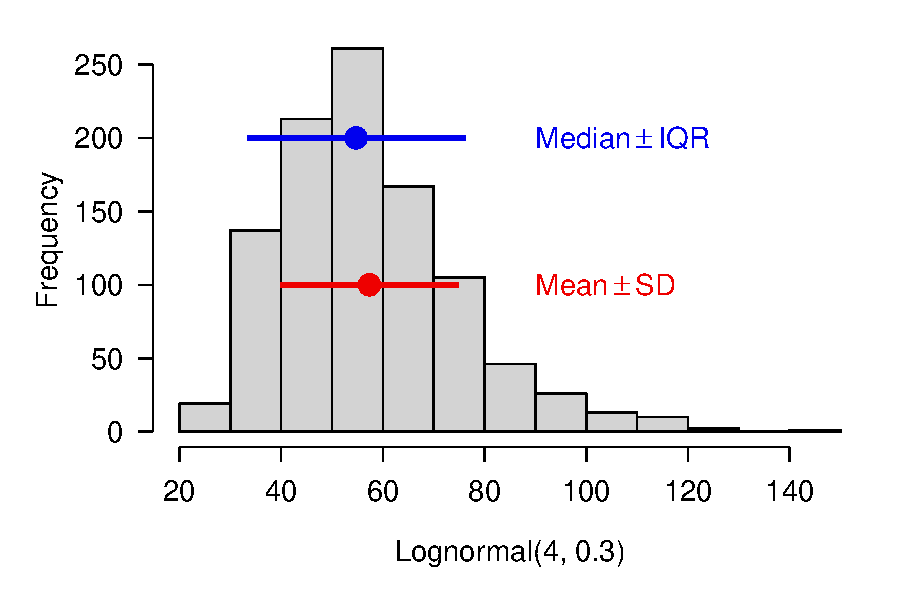
\includegraphics[keepaspectratio]{chapters/ch06_files/figure-pdf/unnamed-chunk-16-1.pdf}}

The \textbf{range} of a variable is the interval defined by its minimum
and maximum. You can get it with function \texttt{range()}. As always,
you may need to handle missing values with \texttt{na.rm=TRUE}.

\begin{Shaded}
\begin{Highlighting}[]
\CommentTok{\# range of a variable in a data frame}
\FunctionTok{range}\NormalTok{(iris}\SpecialCharTok{$}\NormalTok{Petal.Length)}
\end{Highlighting}
\end{Shaded}

\begin{verbatim}
[1] 1.0 6.9
\end{verbatim}

\begin{Shaded}
\begin{Highlighting}[]
\CommentTok{\# make a vector with some numbers and a missing value}
\NormalTok{a }\OtherTok{\textless{}{-}} \FunctionTok{c}\NormalTok{(}\FunctionTok{rnorm}\NormalTok{(}\DecValTok{10}\NormalTok{), }\ConstantTok{NA}\NormalTok{)}

\CommentTok{\# returns NA}
\FunctionTok{range}\NormalTok{(a)}
\end{Highlighting}
\end{Shaded}

\begin{verbatim}
[1] NA NA
\end{verbatim}

\begin{Shaded}
\begin{Highlighting}[]
\CommentTok{\# returns range of non{-}NA values}
\FunctionTok{range}\NormalTok{(a, }\AttributeTok{na.rm=}\ConstantTok{TRUE}\NormalTok{)}
\end{Highlighting}
\end{Shaded}

\begin{verbatim}
[1] -2.549343  2.416207
\end{verbatim}

\section{Covariance and correlation}\label{sec-desc-co}

If anyone knows anything about statistics, or thinks they do, they know
the phrase ``Correlation does not equal causation''. And that statement
is true, both literally and philosophically. \textbf{Correlation} means
that two sets of values tend to change together: larger values of one
variable are associated with larger values of the other variable. Or,
large values of one variable are associated with smaller values of the
other variable. All this means is that the values seem to reliably
change together. Actually demonstrating that one variable is causing
another takes careful observation, experiments, and a different kind of
analysis than correlation.

Despite the fact that correlation does not necessarily imply causation,
a correlation can indicate that something interesting is going on. Maybe
one variable really is causing the other. Maybe both variables are
secretly correlated with a third variable, which explains them both. For
example, in animals the length of the tibia may be correlated with the
mass of the hippocampus. What do these have to do with each other?
Probably nothing. So why are they correlated?

Because bigger animals have bigger parts\ldots just because they are
bigger! Both tibia length and hippocampus mass probably correlate well
with body length, or body mass, measures of \emph{overall} size. Here
noticing a correlation didn't get us anywhere. We had to use biological
reasoning to interpret the numerical result.

Correlation comes in two flavors. The first, \textbf{linear
correlation}, assumes that a relationship between two variables is
linear--that is, a plot of one variable against another approximates a
straight line. The second flavor, \textbf{nonlinear correlation},
assumes only that two variables change together and does not assume any
particular shape to that relationship.

\textbf{Correlation} is a statistical relationship where changes in one
variable are reliably associated with changes in another variable. This
relationship need not be causal, hence the famous mantra, ``correlation
does not equal causation''. As such, correlation is usually a
\textbf{descriptive technique}, which lets researchers characterize
patterns, rather than an \textbf{inferential technique}, which lets
researchers make estimates about unknown parameters (i.e., infer
unobserved quantities).

Correlations are typically expressed as a \textbf{correlation
coefficient}, a value that indicates the strength of the correlation by
its magnitude and the direction of the correlation by its sign.

\begin{itemize}
\item
  \textbf{Positive correlation:} as one variable gets larger, the other
  variable does too. Correlation coefficient approaches \(+1\).
\item
  \textbf{Negative correlation:} as one variable gets larger, the other
  variable gets smaller. Correlation coefficient approaches \(-1\).
\end{itemize}

When a correlation coefficient is near 0, this indicates no correlation.

\begin{figure}

\caption{\label{fig-correlations}Illustration of possible positive and
negative relationships between pairs of variables, with different levels
of consistency (\emph{r}).}

\centering{

\pandocbounded{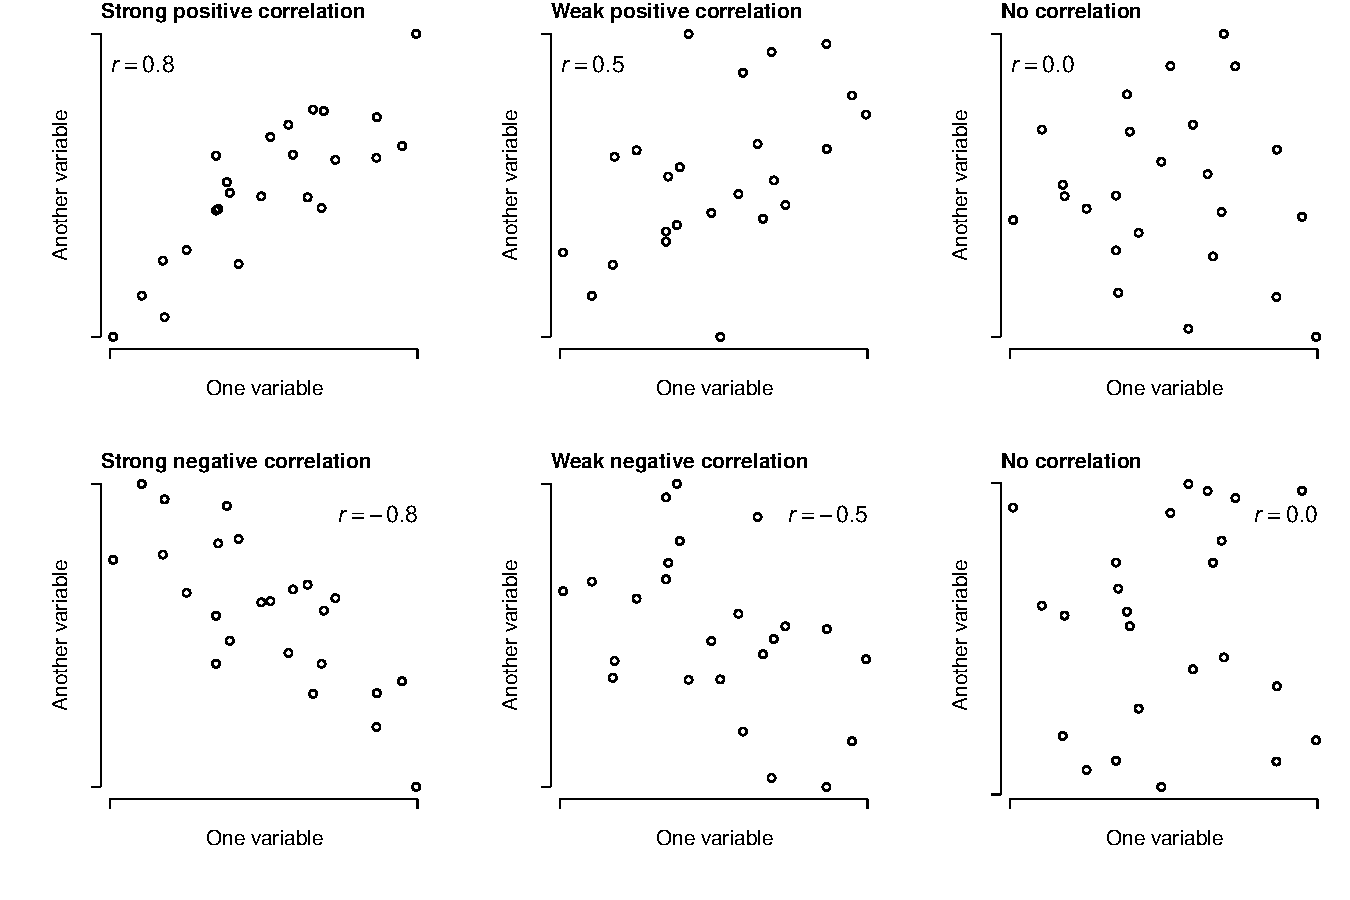
\includegraphics[keepaspectratio,alt={Illustration of possible positive and negative relationships between pairs of variables, with different levels of consistency (r).}]{chapters/ch06_files/figure-pdf/fig-correlations-1.pdf}}

}

\end{figure}%

\subsection{Linear correlation}\label{sec-desc-co-lin}

When we suspect that two variables are correlated, and that the shape of
that relationship is a straight line, we can use \textbf{Pearson's
product moment correlation}, also called \textbf{Pearson's \emph{r}}.

\begin{Shaded}
\begin{Highlighting}[]
\CommentTok{\# calculate linear correlation coefficient}
\FunctionTok{cor}\NormalTok{(iris}\SpecialCharTok{$}\NormalTok{Petal.Length, iris}\SpecialCharTok{$}\NormalTok{Petal.Width)}
\end{Highlighting}
\end{Shaded}

\begin{verbatim}
[1] 0.9628654
\end{verbatim}

You can also request a significance test on the coefficient, although
some might consider this unnecessary because correlation is inherently a
descriptive technique. If you are using correlation as a hypothesis
test, however, you do need a \emph{p}-value.

\begin{Shaded}
\begin{Highlighting}[]
\FunctionTok{cor.test}\NormalTok{(iris}\SpecialCharTok{$}\NormalTok{Petal.Length, iris}\SpecialCharTok{$}\NormalTok{Petal.Width)}
\end{Highlighting}
\end{Shaded}

\begin{verbatim}

    Pearson's product-moment correlation

data:  iris$Petal.Length and iris$Petal.Width
t = 43.387, df = 148, p-value < 2.2e-16
alternative hypothesis: true correlation is not equal to 0
95 percent confidence interval:
 0.9490525 0.9729853
sample estimates:
      cor 
0.9628654 
\end{verbatim}

One of the neat features of \texttt{cor()} is that you can get a
correlation matrix showing the correlation coefficients between many
pairs of variable at once.

\begin{Shaded}
\begin{Highlighting}[]
\CommentTok{\# correlation matrix between the numerical variables in iris}
\FunctionTok{cor}\NormalTok{(iris[,}\DecValTok{1}\SpecialCharTok{:}\DecValTok{4}\NormalTok{])}
\end{Highlighting}
\end{Shaded}

\begin{verbatim}
             Sepal.Length Sepal.Width Petal.Length Petal.Width
Sepal.Length    1.0000000  -0.1175698    0.8717538   0.8179411
Sepal.Width    -0.1175698   1.0000000   -0.4284401  -0.3661259
Petal.Length    0.8717538  -0.4284401    1.0000000   0.9628654
Petal.Width     0.8179411  -0.3661259    0.9628654   1.0000000
\end{verbatim}

Here we see that each variable is perfectly correlated with itself (the
1s on the diagonal). Sepal length and sepal width are negatively
correlated (\texttt{-0.1175698}) while petal length and petal width are
strongly positively correlated (\texttt{0.8717538}). You only need to
report correlation coefficients to 2 or 3 decimal places.

There isn't a built-in way to check for significant correlations between
many pairs of variables at once. This is because \texttt{cor.test()}
only works with one pair at a time. Fortunately, it's not hard to do in
a loop:

\begin{Shaded}
\begin{Highlighting}[]
\CommentTok{\# data frame with just the numeric variables}
\NormalTok{dx }\OtherTok{\textless{}{-}}\NormalTok{ iris[,}\DecValTok{1}\SpecialCharTok{:}\DecValTok{4}\NormalTok{]}

\CommentTok{\# set up data frame to hold results}
\CommentTok{\# combn(..., 2) returns matrix of all unique pairs of names}
\CommentTok{\# t(ranspose) this and turn into a data frame.}
\NormalTok{cor.df }\OtherTok{\textless{}{-}} \FunctionTok{as.data.frame}\NormalTok{(}\FunctionTok{t}\NormalTok{(}\FunctionTok{combn}\NormalTok{(}\FunctionTok{names}\NormalTok{(dx), }\DecValTok{2}\NormalTok{)))}
\NormalTok{cor.df}\SpecialCharTok{$}\NormalTok{r }\OtherTok{\textless{}{-}} \ConstantTok{NA}
\NormalTok{cor.df}\SpecialCharTok{$}\NormalTok{p }\OtherTok{\textless{}{-}} \ConstantTok{NA}

\CommentTok{\# find the r and p values in a loop}
\ControlFlowTok{for}\NormalTok{(i }\ControlFlowTok{in} \DecValTok{1}\SpecialCharTok{:}\FunctionTok{nrow}\NormalTok{(cor.df))\{}
  \CommentTok{\# test once per iteration  }
\NormalTok{  curr }\OtherTok{\textless{}{-}} \FunctionTok{cor.test}\NormalTok{(dx[,cor.df}\SpecialCharTok{$}\NormalTok{V1[i]], dx[,cor.df}\SpecialCharTok{$}\NormalTok{V2[i]])}
  \CommentTok{\# pull out values we need from correlation test result}
  \CommentTok{\# and round to 3 decimal places}
\NormalTok{  cor.df}\SpecialCharTok{$}\NormalTok{r[i] }\OtherTok{\textless{}{-}} \FunctionTok{round}\NormalTok{(curr}\SpecialCharTok{$}\NormalTok{estimate,}\DecValTok{3}\NormalTok{)}
\NormalTok{  cor.df}\SpecialCharTok{$}\NormalTok{p[i] }\OtherTok{\textless{}{-}} \FunctionTok{round}\NormalTok{(curr}\SpecialCharTok{$}\NormalTok{p.value, }\DecValTok{3}\NormalTok{)}
\NormalTok{\}}\CommentTok{\#close i loop}

\CommentTok{\# print result}
\NormalTok{cor.df}
\end{Highlighting}
\end{Shaded}

\begin{verbatim}
            V1           V2      r     p
1 Sepal.Length  Sepal.Width -0.118 0.152
2 Sepal.Length Petal.Length  0.872 0.000
3 Sepal.Length  Petal.Width  0.818 0.000
4  Sepal.Width Petal.Length -0.428 0.000
5  Sepal.Width  Petal.Width -0.366 0.000
6 Petal.Length  Petal.Width  0.963 0.000
\end{verbatim}

If you want to visualize many potential correlations at once, you can
construct a \textbf{scatterplot matrix} using function \texttt{pairs()}.
This will plot every pair of variables in a data frame. We are going
borrow a function called \texttt{panel.cor()} from the \texttt{pairs()}
help page so that we get both the scatterplots \emph{and} the linear
correlation coefficients.

\begin{Shaded}
\begin{Highlighting}[]
\CommentTok{\# from ?pairs}
\CommentTok{\# just paste this in once to define the function}
\CommentTok{\# try changing some arguments to change the behavior!}
\NormalTok{panel.cor }\OtherTok{\textless{}{-}} \ControlFlowTok{function}\NormalTok{(x, y, }\AttributeTok{digits =} \DecValTok{2}\NormalTok{, }\AttributeTok{prefix =} \StringTok{""}\NormalTok{, cex.cor, ...)}
\NormalTok{\{}
    \FunctionTok{par}\NormalTok{(}\AttributeTok{usr =} \FunctionTok{c}\NormalTok{(}\DecValTok{0}\NormalTok{, }\DecValTok{1}\NormalTok{, }\DecValTok{0}\NormalTok{, }\DecValTok{1}\NormalTok{))}
\NormalTok{    r }\OtherTok{\textless{}{-}} \FunctionTok{abs}\NormalTok{(}\FunctionTok{cor}\NormalTok{(x, y))}
\NormalTok{    txt }\OtherTok{\textless{}{-}} \FunctionTok{format}\NormalTok{(}\FunctionTok{c}\NormalTok{(r, }\FloatTok{0.123456789}\NormalTok{), }\AttributeTok{digits =}\NormalTok{ digits)[}\DecValTok{1}\NormalTok{]}
\NormalTok{    txt }\OtherTok{\textless{}{-}} \FunctionTok{paste0}\NormalTok{(prefix, txt)}
    \ControlFlowTok{if}\NormalTok{(}\FunctionTok{missing}\NormalTok{(cex.cor)) cex.cor }\OtherTok{\textless{}{-}} \FloatTok{0.8}\SpecialCharTok{/}\FunctionTok{strwidth}\NormalTok{(txt)}
    \FunctionTok{text}\NormalTok{(}\FloatTok{0.5}\NormalTok{, }\FloatTok{0.5}\NormalTok{, txt, }\AttributeTok{cex =}\NormalTok{ cex.cor }\SpecialCharTok{*}\NormalTok{ r)}
\NormalTok{\}}

\CommentTok{\# make the scatterplot matrix}
\FunctionTok{pairs}\NormalTok{(iris[,}\DecValTok{1}\SpecialCharTok{:}\DecValTok{4}\NormalTok{], }\AttributeTok{lower.panel=}\NormalTok{panel.smooth, }\AttributeTok{upper.panel=}\NormalTok{panel.cor, }\AttributeTok{gap=}\DecValTok{0}\NormalTok{)}
\end{Highlighting}
\end{Shaded}

\begin{figure}[H]

\caption{\label{fig-scatterplotmatrix}Scatterplot matrix showing
possible correlations between the numeric variables in the \texttt{iris}
data frame.}

\centering{

\pandocbounded{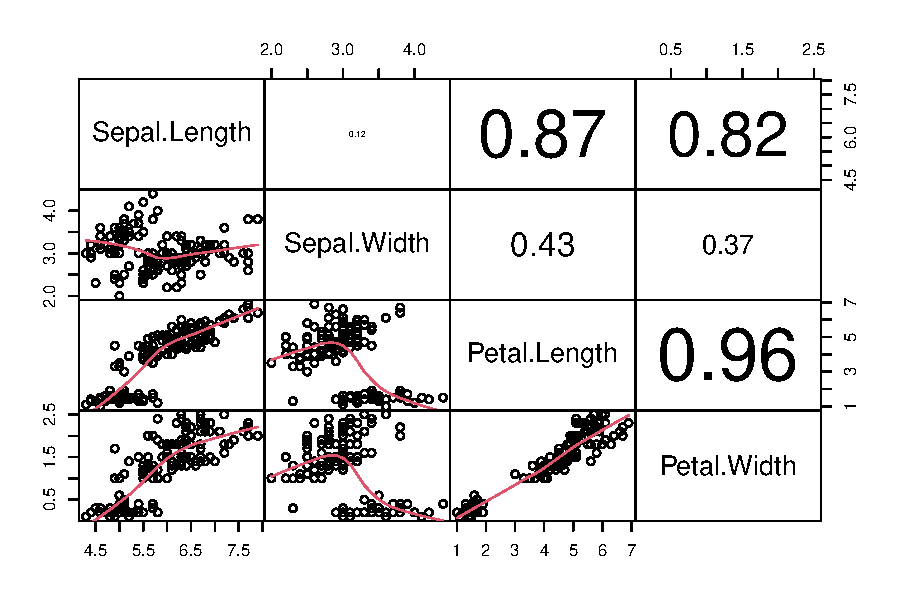
\includegraphics[keepaspectratio,alt={Scatterplot matrix showing possible correlations between the numeric variables in the `iris` data frame.}]{chapters/ch06_files/figure-pdf/fig-scatterplotmatrix-1.pdf}}

}

\end{figure}%

In this figure, scatterplots in the lower triangle correspond to the
variables in the diagonal whom they intersect. For example, the far left
and far bottom scatterplot has Sepal.Length for its horizontal axis, and
Petal.Width for its vertical axis. Go one panel to the right, and the
horizontal axis is now Sepal.Width. The correlation coefficients in the
upper triangle are identified the same way. For example, the large 0.96
on the far right, 3rd panel down, is the correlation coefficient between
Petal.Length and Petal.Width.

\subsection{Nonlinear correlation}\label{sec-desc-co-non}

Many processes and relationships in biology are not linear, and
sometimes we want to calculate correlation coefficients for those
relationships. Consider the figure below. The left panel clearly shows
some relationship between \(X\) and \(Y\), but it is not linear and
using a linear correlation coefficient might miss something.

\begin{figure}

\caption{\label{fig-nonlinear}Left: illustration of a nonlinear
correlation. Right: When values are rank-transformed, the nonlinear
trend becomes linear.}

\centering{

\pandocbounded{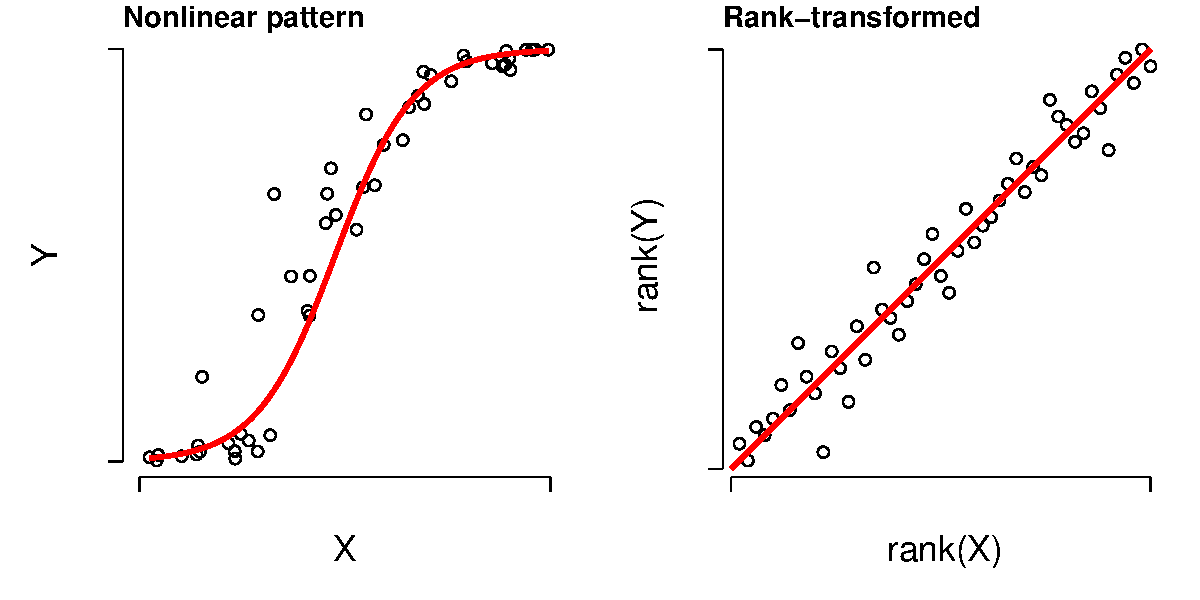
\includegraphics[keepaspectratio,alt={Left: illustration of a nonlinear correlation. Right: When values are rank-transformed, the nonlinear trend becomes linear.}]{chapters/ch06_files/figure-pdf/fig-nonlinear-1.pdf}}

}

\end{figure}%

However, if you \textbf{rank-transform} the data, the relationship often
turns into something more linear. A ``rank-transform'' assigns the
smallest value value 0, the second smallest value to 1, and so on.
Rank-transforming these data lets us calculate a nonparametric,
nonlinear correlation. The nonparametric equivalent of Pearson's
\emph{r} is \textbf{Spearman's \(\rho\)} (``rho''). It can be obtained
using code similar to that for linear correlation.

\begin{Shaded}
\begin{Highlighting}[]
\CommentTok{\# just the correlation}
\FunctionTok{cor}\NormalTok{(iris}\SpecialCharTok{$}\NormalTok{Petal.Length, iris}\SpecialCharTok{$}\NormalTok{Sepal.Width, }\AttributeTok{method=}\StringTok{"spearman"}\NormalTok{)}
\end{Highlighting}
\end{Shaded}

\begin{verbatim}
[1] -0.3096351
\end{verbatim}

\begin{Shaded}
\begin{Highlighting}[]
\CommentTok{\# significance test}
\FunctionTok{cor.test}\NormalTok{(iris}\SpecialCharTok{$}\NormalTok{Petal.Length, iris}\SpecialCharTok{$}\NormalTok{Sepal.Width, }\AttributeTok{method=}\StringTok{"spearman"}\NormalTok{)}
\end{Highlighting}
\end{Shaded}

\begin{verbatim}

    Spearman's rank correlation rho

data:  iris$Petal.Length and iris$Sepal.Width
S = 736637, p-value = 0.0001154
alternative hypothesis: true rho is not equal to 0
sample estimates:
       rho 
-0.3096351 
\end{verbatim}

When you run a nonlinear correlation test, you will often get the
warning
\texttt{Warning\ in\ cor.test.default\ ...\ :\ Cannot\ compute\ exact\ p-value\ with\ ties}.
All this means is that some of the rankings are tied. This warning can
be safely ignored.

\chapter{Summarizing biological data}\label{sec-summ}

In the last module we saw how single variables can be described or
summarized using descriptive statistics (see Chapter~\ref{sec-desc}). In
this chapter we will extend that to summarizing values by groups.
Indeed, comparing the mean values in different groups is one of the most
important types of tests we do in biology (see
Chapter~\ref{sec-groups}).

\section{Summarizing a data frame}\label{sec-summ-df}

You can get a quick numerical summary of a vector or a dataset with
\texttt{summary()}. The examples below use the built-in dataset
\texttt{iris}.

\begin{Shaded}
\begin{Highlighting}[]
\CommentTok{\# summarize a data frame}
\FunctionTok{summary}\NormalTok{(iris)}
\end{Highlighting}
\end{Shaded}

\begin{verbatim}
  Sepal.Length    Sepal.Width     Petal.Length    Petal.Width   
 Min.   :4.300   Min.   :2.000   Min.   :1.000   Min.   :0.100  
 1st Qu.:5.100   1st Qu.:2.800   1st Qu.:1.600   1st Qu.:0.300  
 Median :5.800   Median :3.000   Median :4.350   Median :1.300  
 Mean   :5.843   Mean   :3.057   Mean   :3.758   Mean   :1.199  
 3rd Qu.:6.400   3rd Qu.:3.300   3rd Qu.:5.100   3rd Qu.:1.800  
 Max.   :7.900   Max.   :4.400   Max.   :6.900   Max.   :2.500  
       Species  
 setosa    :50  
 versicolor:50  
 virginica :50  
                
                
                
\end{verbatim}

\begin{Shaded}
\begin{Highlighting}[]
\CommentTok{\# summarize a single variable}
\FunctionTok{summary}\NormalTok{(iris}\SpecialCharTok{$}\NormalTok{Petal.Length)}
\end{Highlighting}
\end{Shaded}

\begin{verbatim}
   Min. 1st Qu.  Median    Mean 3rd Qu.    Max. 
  1.000   1.600   4.350   3.758   5.100   6.900 
\end{verbatim}

The function \texttt{summary()} has methods for many other types of R
objects such as \texttt{glm}, \texttt{lm}, \texttt{aov}, and so on.

\subsection{Summarizing by groups (AKA: pivot
tables)}\label{sec-summ-agg}

One of the most common data operations is \textbf{aggregation}, or
\textbf{summarization by groups}. In Excel, this is done using
\textbf{Pivot Tables}. In R, the functions \texttt{aggregate()} and
\texttt{tapply()} are used for pivot table-like functionality. The
\texttt{tidyverse} equivalent for \texttt{aggregate()} and
\texttt{tapply()} is \texttt{dplyr::summarise()}. All of these can be
much more powerful than an Excel pivot table because while Excel pivot
tables are limited to a small set of built-in functions, R can aggregate
by any function.

\begin{figure}[H]

\caption{Example of a pivot table in Excel}

{\centering \pandocbounded{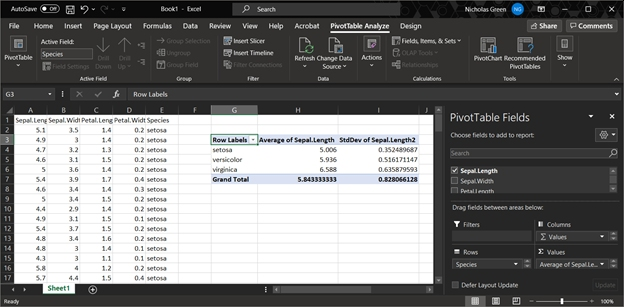
\includegraphics[keepaspectratio,alt={Pivot table in Excel calculating the mean and SD of sepal length from the iris dataset.}]{chapters/../images/07-01.jpg}}

}

\end{figure}%

\subsubsection{\texorpdfstring{\texttt{aggregate()}}{aggregate()}}\label{aggregate}

The base R workhorse for summarizing data by groups is
\texttt{aggregate()}. It is straightforward and powerful enough to cover
almost all use cases. The most important inputs to \texttt{aggregate()}
are the data to be summarized, the variable or variables that define the
groups, and the function by which to summarize. The examples below shows
how to calculate the mean petal length for each species in the
\texttt{iris} dataset.

If the variable to be summarized and the grouping variables are in the
same data frame (which is usually the case), you can use the formula
interface to \texttt{aggregate()}; otherwise, use the \texttt{by=}
interface.

\begin{Shaded}
\begin{Highlighting}[]
\CommentTok{\# example using by=}
\FunctionTok{aggregate}\NormalTok{(iris}\SpecialCharTok{$}\NormalTok{Petal.Length,}
          \AttributeTok{by=}\FunctionTok{list}\NormalTok{(iris}\SpecialCharTok{$}\NormalTok{Species),}
\NormalTok{          mean)}
\end{Highlighting}
\end{Shaded}

\begin{verbatim}
     Group.1     x
1     setosa 1.462
2 versicolor 4.260
3  virginica 5.552
\end{verbatim}

\begin{Shaded}
\begin{Highlighting}[]
\CommentTok{\# better method using formula}
\FunctionTok{aggregate}\NormalTok{(Petal.Length}\SpecialCharTok{\textasciitilde{}}\NormalTok{Species,}
          \AttributeTok{data=}\NormalTok{iris,}
\NormalTok{          mean)}
\end{Highlighting}
\end{Shaded}

\begin{verbatim}
     Species Petal.Length
1     setosa        1.462
2 versicolor        4.260
3  virginica        5.552
\end{verbatim}

The formula interface is cleaner and easier than the \texttt{by=}
interface (first example), and has the key advantage that it
automatically passes variable names to the result. If you use
\texttt{by=} you may want to rename the columns in the result.

In my own code I prefer to name my aggregation tables \texttt{agg}, with
additional parts like \texttt{agg1}, \texttt{agg.fish}, and so on if
needed. Function \texttt{aggregate()} produces a data frame with a
column for each grouping variable (\texttt{Group.1}, \texttt{Group.2}
and so on) and a single column \texttt{x} containing the summarized
values. We can use this property to construct tables that summarize by
more than one variable.

\begin{Shaded}
\begin{Highlighting}[]
\CommentTok{\# spare copy}
\NormalTok{x }\OtherTok{\textless{}{-}}\NormalTok{ iris}

\CommentTok{\# add another grouping variable}
\NormalTok{x}\SpecialCharTok{$}\NormalTok{color }\OtherTok{\textless{}{-}} \FunctionTok{c}\NormalTok{(}\StringTok{"red"}\NormalTok{, }\StringTok{"white"}\NormalTok{)}

\CommentTok{\# by= example: notice how columns in result need to be renamed}
\NormalTok{agg }\OtherTok{\textless{}{-}} \FunctionTok{aggregate}\NormalTok{(x}\SpecialCharTok{$}\NormalTok{Petal.Length,}
                 \AttributeTok{by=}\FunctionTok{list}\NormalTok{(x}\SpecialCharTok{$}\NormalTok{Species, x}\SpecialCharTok{$}\NormalTok{color),}
\NormalTok{                 mean)}
\NormalTok{agg}
\end{Highlighting}
\end{Shaded}

\begin{verbatim}
     Group.1 Group.2     x
1     setosa     red 1.456
2 versicolor     red 4.308
3  virginica     red 5.564
4     setosa   white 1.468
5 versicolor   white 4.212
6  virginica   white 5.540
\end{verbatim}

\begin{Shaded}
\begin{Highlighting}[]
\CommentTok{\# change column names}
\FunctionTok{names}\NormalTok{(agg) }\OtherTok{\textless{}{-}} \FunctionTok{c}\NormalTok{(}\StringTok{"spp"}\NormalTok{, }\StringTok{"color"}\NormalTok{, }\StringTok{"mean"}\NormalTok{)}
\NormalTok{agg}
\end{Highlighting}
\end{Shaded}

\begin{verbatim}
         spp color  mean
1     setosa   red 1.456
2 versicolor   red 4.308
3  virginica   red 5.564
4     setosa white 1.468
5 versicolor white 4.212
6  virginica white 5.540
\end{verbatim}

\begin{Shaded}
\begin{Highlighting}[]
\CommentTok{\# formula example: much easier}
\NormalTok{agg }\OtherTok{\textless{}{-}} \FunctionTok{aggregate}\NormalTok{(Petal.Length}\SpecialCharTok{\textasciitilde{}}\NormalTok{Species}\SpecialCharTok{+}\NormalTok{color, }\AttributeTok{data=}\NormalTok{x, mean)}
\NormalTok{agg}
\end{Highlighting}
\end{Shaded}

\begin{verbatim}
     Species color Petal.Length
1     setosa   red        1.456
2 versicolor   red        4.308
3  virginica   red        5.564
4     setosa white        1.468
5 versicolor white        4.212
6  virginica white        5.540
\end{verbatim}

Notice that in \texttt{agg} the values are sorted by the grouping
variables from right to left: in this example, by \texttt{color}, then
\texttt{Species}. This is the reverse of the order in the original
command. The result of \texttt{aggregate()} is a data frame, so data
within it can be rearranged using \texttt{order()}.

Often we want to summarize a variable by multiple functions--for
example, to get a table with the mean and SD in each group. My preferred
way to do this is to use several \texttt{aggregate()} commands, and then
combine the results. The examples below shows two ways to construct a
table with the mean and SD of a variable.

\begin{Shaded}
\begin{Highlighting}[]
\CommentTok{\# define a formula and save some typing:}
\NormalTok{f1 }\OtherTok{\textless{}{-}} \FunctionTok{formula}\NormalTok{(Petal.Length}\SpecialCharTok{\textasciitilde{}}\NormalTok{Species)}

\CommentTok{\# method 1: single table using formula}
\NormalTok{agg }\OtherTok{\textless{}{-}} \FunctionTok{aggregate}\NormalTok{(f1, }\AttributeTok{data=}\NormalTok{x, mean)}
\NormalTok{agg}\SpecialCharTok{$}\NormalTok{sd }\OtherTok{\textless{}{-}} \FunctionTok{aggregate}\NormalTok{(f1, }\AttributeTok{data=}\NormalTok{x, sd)}\SpecialCharTok{$}\NormalTok{Petal.Length}
\FunctionTok{names}\NormalTok{(agg)[}\FunctionTok{which}\NormalTok{(}\FunctionTok{names}\NormalTok{(agg) }\SpecialCharTok{==} \StringTok{"Petal.Length"}\NormalTok{)] }\OtherTok{\textless{}{-}} \StringTok{"mn"}

\NormalTok{agg}
\end{Highlighting}
\end{Shaded}

\begin{verbatim}
     Species    mn        sd
1     setosa 1.462 0.1736640
2 versicolor 4.260 0.4699110
3  virginica 5.552 0.5518947
\end{verbatim}

The \texttt{\$Petal.Length} on the end of \texttt{aggregate()} is
important because we want only column \texttt{Petal.Length} of the
output. Without \texttt{\$Petal.Length}, the result will be messy when
we try to add it to \texttt{agg}. If you ever want to do this with the
\texttt{by=} method, the column of the output containing the summarized
values will be named \texttt{x}.

\begin{Shaded}
\begin{Highlighting}[]
\CommentTok{\# method 1a: single table, using by=}
\NormalTok{agg }\OtherTok{\textless{}{-}} \FunctionTok{aggregate}\NormalTok{(iris}\SpecialCharTok{$}\NormalTok{Petal.Length, }\AttributeTok{by=}\FunctionTok{list}\NormalTok{(iris}\SpecialCharTok{$}\NormalTok{Species), mean)}
\DocumentationTok{\#\# note use of $x:}
\NormalTok{agg}\SpecialCharTok{$}\NormalTok{sd }\OtherTok{\textless{}{-}} \FunctionTok{aggregate}\NormalTok{(iris}\SpecialCharTok{$}\NormalTok{Petal.Length, }\AttributeTok{by=}\FunctionTok{list}\NormalTok{(iris}\SpecialCharTok{$}\NormalTok{Species), sd)}\SpecialCharTok{$}\NormalTok{x}

\CommentTok{\# change names in result:}
\FunctionTok{names}\NormalTok{(agg)[}\FunctionTok{which}\NormalTok{(}\FunctionTok{names}\NormalTok{(agg) }\SpecialCharTok{==} \StringTok{"x"}\NormalTok{)] }\OtherTok{\textless{}{-}} \StringTok{"mn"}
\FunctionTok{names}\NormalTok{(agg)[}\FunctionTok{which}\NormalTok{(}\FunctionTok{names}\NormalTok{(agg) }\SpecialCharTok{==} \StringTok{"Group.1"}\NormalTok{)] }\OtherTok{\textless{}{-}} \StringTok{"species"}
\NormalTok{agg}
\end{Highlighting}
\end{Shaded}

\begin{verbatim}
     species    mn        sd
1     setosa 1.462 0.1736640
2 versicolor 4.260 0.4699110
3  virginica 5.552 0.5518947
\end{verbatim}

The second approach is to make several \texttt{aggregate()} tables, and
combine them into a single result.

\begin{Shaded}
\begin{Highlighting}[]
\CommentTok{\# method 2: multiple tables}
\CommentTok{\#           (note: there are lots of ways to do this)}
\NormalTok{agg.mn }\OtherTok{\textless{}{-}} \FunctionTok{aggregate}\NormalTok{(f1, }\AttributeTok{data=}\NormalTok{x, mean)}
\NormalTok{agg.sd }\OtherTok{\textless{}{-}} \FunctionTok{aggregate}\NormalTok{(f1, }\AttributeTok{data=}\NormalTok{x, sd)}
\NormalTok{agg }\OtherTok{\textless{}{-}} \FunctionTok{data.frame}\NormalTok{(agg.mn, }\AttributeTok{sd=}\NormalTok{agg.sd}\SpecialCharTok{$}\NormalTok{Petal.Length)}
\FunctionTok{names}\NormalTok{(agg)[}\DecValTok{2}\NormalTok{] }\OtherTok{\textless{}{-}} \StringTok{"mn"}
\NormalTok{agg}
\end{Highlighting}
\end{Shaded}

\begin{verbatim}
     Species    mn        sd
1     setosa 1.462 0.1736640
2 versicolor 4.260 0.4699110
3  virginica 5.552 0.5518947
\end{verbatim}

\subsubsection{\texorpdfstring{\texttt{tapply()}}{tapply()}}\label{tapply}

The base function \texttt{tapply()}, like \texttt{aggregate()},
summarizes a numeric variable by a grouping variable. In fact,
\texttt{aggregate()} uses \texttt{tapply()} internally. The difference
is that while \texttt{aggregate()} returns a data frame,
\texttt{tapply()} returns an array with number of dimensions equal to
the number of grouping variables. The inputs are a vector to be
summarized, a grouping variable or set of variables, and the function by
which to summarize.

\begin{Shaded}
\begin{Highlighting}[]

\CommentTok{\# spare copy}
\NormalTok{x }\OtherTok{\textless{}{-}}\NormalTok{ iris}
\CommentTok{\# add some extra grouping variables}
\NormalTok{x}\SpecialCharTok{$}\NormalTok{color }\OtherTok{\textless{}{-}} \FunctionTok{c}\NormalTok{(}\StringTok{"red"}\NormalTok{, }\StringTok{"white"}\NormalTok{)}
\NormalTok{x}\SpecialCharTok{$}\NormalTok{treat }\OtherTok{\textless{}{-}} \FunctionTok{c}\NormalTok{(}\StringTok{"a"}\NormalTok{, }\StringTok{"b"}\NormalTok{, }\StringTok{"c"}\NormalTok{)}

\CommentTok{\# tapply by 1 variable}
\FunctionTok{tapply}\NormalTok{(x}\SpecialCharTok{$}\NormalTok{Petal.Length, x}\SpecialCharTok{$}\NormalTok{Species, mean)}
\DocumentationTok{\#\#     setosa versicolor  virginica }
\DocumentationTok{\#\#      1.462      4.260      5.552}
\end{Highlighting}
\end{Shaded}

\begin{Shaded}
\begin{Highlighting}[]
\CommentTok{\# tapply by 2 variables}
\FunctionTok{tapply}\NormalTok{(x}\SpecialCharTok{$}\NormalTok{Petal.Length, x[,}\FunctionTok{c}\NormalTok{(}\StringTok{"Species"}\NormalTok{, }\StringTok{"color"}\NormalTok{)], mean)}
\end{Highlighting}
\end{Shaded}

\begin{verbatim}
            color
Species        red white
  setosa     1.456 1.468
  versicolor 4.308 4.212
  virginica  5.564 5.540
\end{verbatim}

\begin{Shaded}
\begin{Highlighting}[]
\NormalTok{\# tapply by 3 variables}
\NormalTok{tapply(x$Petal.Length, x[,c("Species", "color", "treat")], mean)}
\end{Highlighting}
\end{Shaded}

\begin{Shaded}
\begin{Highlighting}[]
\CommentTok{\# vary the arrangement of groups:}
\FunctionTok{tapply}\NormalTok{(x}\SpecialCharTok{$}\NormalTok{Petal.Length, x[,}\FunctionTok{c}\NormalTok{(}\StringTok{"color"}\NormalTok{, }\StringTok{"Species"}\NormalTok{)], mean)}
\end{Highlighting}
\end{Shaded}

\begin{verbatim}
       Species
color   setosa versicolor virginica
  red    1.456      4.308     5.564
  white  1.468      4.212     5.540
\end{verbatim}

Personally, I prefer \texttt{aggregate()} to \texttt{tapply()} because
it is usually more convenient to have the results in a data frame. You
also need to be more careful with \texttt{tapply()} because it will
interpret factors as factors and thus return values for missing levels.
\texttt{aggregate()}, on the other hand, will drop the missing levels.

\begin{Shaded}
\begin{Highlighting}[]
\CommentTok{\# aggregate drops the missing levels.}
\FunctionTok{aggregate}\NormalTok{(Petal.Length}\SpecialCharTok{\textasciitilde{}}\NormalTok{Species, }\AttributeTok{data=}\NormalTok{iris[}\DecValTok{1}\SpecialCharTok{:}\DecValTok{100}\NormalTok{,], mean)}
\end{Highlighting}
\end{Shaded}

\begin{verbatim}
     Species Petal.Length
1     setosa        1.462
2 versicolor        4.260
\end{verbatim}

\begin{Shaded}
\begin{Highlighting}[]
\CommentTok{\# tapply includes the missing levels}
\FunctionTok{tapply}\NormalTok{(iris}\SpecialCharTok{$}\NormalTok{Petal.Length[}\DecValTok{1}\SpecialCharTok{:}\DecValTok{100}\NormalTok{], iris}\SpecialCharTok{$}\NormalTok{Species[}\DecValTok{1}\SpecialCharTok{:}\DecValTok{100}\NormalTok{], mean)}
\end{Highlighting}
\end{Shaded}

\begin{verbatim}
    setosa versicolor  virginica 
     1.462      4.260         NA 
\end{verbatim}

Which behavior you want depends on what you are trying to do. Just be
aware that \texttt{aggregate()} and \texttt{tapply()} might return
different numbers of values depending on what you have already done to
your data frame.

\subsection{Summarizing by arbitrary
functions}\label{summarizing-by-arbitrary-functions}

If you've ever used Excel Pivot Tables, you will have noticed that data
can only be summarized by a limited set of functions. On the other hand,
\texttt{aggregate()} (and \texttt{tapply()}, but we'll focus on
\texttt{aggregate()}) can be used with pretty much any function that
takes in a vector and returns a scalar. You can even write your own
functions! Below are some examples. Notice in the first example that
arguments to the summarizing function follow its name.

\begin{Shaded}
\begin{Highlighting}[]
\CommentTok{\# first quartile (25th percentile)}
\FunctionTok{aggregate}\NormalTok{(Petal.Length}\SpecialCharTok{\textasciitilde{}}\NormalTok{Species, }\AttributeTok{data=}\NormalTok{iris, quantile, }\FloatTok{0.25}\NormalTok{)}
\end{Highlighting}
\end{Shaded}

\begin{verbatim}
     Species Petal.Length
1     setosa          1.4
2 versicolor          4.0
3  virginica          5.1
\end{verbatim}

\begin{Shaded}
\begin{Highlighting}[]
\CommentTok{\# number of values}
\FunctionTok{aggregate}\NormalTok{(Petal.Length}\SpecialCharTok{\textasciitilde{}}\NormalTok{Species, }\AttributeTok{data=}\NormalTok{iris, length)}
\end{Highlighting}
\end{Shaded}

\begin{verbatim}
     Species Petal.Length
1     setosa           50
2 versicolor           50
3  virginica           50
\end{verbatim}

The following examples illustrate \textbf{anonymous functions}:
functions defined within another function and never defined in the R
workspace. The \texttt{x} in \texttt{function(x)} is taken to be the
values within each group defined by the variable(s) on the right-hand
side of \texttt{\textasciitilde{}} or in \texttt{by=}. Notice that the
end of such a command will need a lot of \texttt{)}, \texttt{\}}, and
sometimes \texttt{{]}}. Using an editor with syntax highlighting is very
helpful!

\begin{Shaded}
\begin{Highlighting}[]
\CommentTok{\# number of missing values}
\FunctionTok{aggregate}\NormalTok{(Petal.Length}\SpecialCharTok{\textasciitilde{}}\NormalTok{Species,}
          \AttributeTok{data=}\NormalTok{iris,}
          \ControlFlowTok{function}\NormalTok{(x)\{}\FunctionTok{length}\NormalTok{(}\FunctionTok{which}\NormalTok{(}\FunctionTok{is.na}\NormalTok{(x)))\})}
\end{Highlighting}
\end{Shaded}

\begin{verbatim}
     Species Petal.Length
1     setosa            0
2 versicolor            0
3  virginica            0
\end{verbatim}

\begin{Shaded}
\begin{Highlighting}[]
\CommentTok{\# number of non{-}missing values}
\FunctionTok{aggregate}\NormalTok{(Petal.Length}\SpecialCharTok{\textasciitilde{}}\NormalTok{Species, }
          \AttributeTok{data=}\NormalTok{iris,}
          \ControlFlowTok{function}\NormalTok{(x)\{}\FunctionTok{length}\NormalTok{(}\FunctionTok{which}\NormalTok{(}\SpecialCharTok{!}\FunctionTok{is.na}\NormalTok{(x)))\})}
\end{Highlighting}
\end{Shaded}

\begin{verbatim}
     Species Petal.Length
1     setosa           50
2 versicolor           50
3  virginica           50
\end{verbatim}

\begin{Shaded}
\begin{Highlighting}[]
\CommentTok{\# number of values \textgreater{}= 2}
\FunctionTok{aggregate}\NormalTok{(Petal.Length}\SpecialCharTok{\textasciitilde{}}\NormalTok{Species,}
          \AttributeTok{data=}\NormalTok{iris,}
          \ControlFlowTok{function}\NormalTok{(x)\{}\FunctionTok{length}\NormalTok{(}\FunctionTok{which}\NormalTok{(x }\SpecialCharTok{\textgreater{}=} \DecValTok{2}\NormalTok{))\})}
\end{Highlighting}
\end{Shaded}

\begin{verbatim}
     Species Petal.Length
1     setosa            0
2 versicolor           50
3  virginica           50
\end{verbatim}

\begin{Shaded}
\begin{Highlighting}[]
\CommentTok{\# number of UNIQUE values \textgreater{}= 2}
\FunctionTok{aggregate}\NormalTok{(Petal.Length}\SpecialCharTok{\textasciitilde{}}\NormalTok{Species,}
          \AttributeTok{data=}\NormalTok{iris,}
          \ControlFlowTok{function}\NormalTok{(x)\{}\FunctionTok{length}\NormalTok{(}\FunctionTok{unique}\NormalTok{(x[}\FunctionTok{which}\NormalTok{(x }\SpecialCharTok{\textgreater{}=} \DecValTok{2}\NormalTok{)]))\})}
\end{Highlighting}
\end{Shaded}

\begin{verbatim}
     Species Petal.Length
1     setosa            0
2 versicolor           19
3  virginica           20
\end{verbatim}

Being able to use almost any function, and to define your own functions,
makes \texttt{aggregate()} an immensely powerful tool to have in your R
toolbox.

\section{\texorpdfstring{The \texttt{apply()}
family}{The apply() family}}\label{the-apply-family}

The \texttt{apply()} family is a group of functions that operate over
the \textbf{dimensions} or \textbf{margins} an object. You can use the
\texttt{apply()} family to summarize across rows or columns, or across
elements of a list, and so on. The function used most often is
\texttt{apply()}, which works on data frames, matrices and arrays. There
are also \texttt{lapply()}, which works on lists and returns a list;
\texttt{sapply()}, which operates on lists and returns the simplest
object possible; and a few others.

We already saw \texttt{tapply()}, which works on subsets of a data frame
or array.

\subsection{\texorpdfstring{\texttt{apply()} for arrays and data
frames}{apply() for arrays and data frames}}\label{apply-for-arrays-and-data-frames}

Function \texttt{apply()} works on data frames or arrays with \(\ge2\)
dimensions. Its arguments are the object to be operated on, the margin
(or dimension) on which to operate, and the operation (or function). The
first margin is rows, the second is columns, and so on. The result of
\texttt{apply()} will \emph{always} have one fewer dimension than the
input.

Some typical \texttt{apply()} commands are demonstrated below. The first
calculates the sum of values in each row (margin \texttt{1}) of its
input \texttt{x}.

\begin{Shaded}
\begin{Highlighting}[]
\CommentTok{\# test dataset with only numeric values}
\NormalTok{x }\OtherTok{\textless{}{-}}\NormalTok{ iris[,}\DecValTok{1}\SpecialCharTok{:}\DecValTok{4}\NormalTok{]}

\CommentTok{\# margin 1 = rows {-}{-}\textgreater{} row sums}
\FunctionTok{apply}\NormalTok{(x, }\DecValTok{1}\NormalTok{, sum)}
\end{Highlighting}
\end{Shaded}

\begin{verbatim}
  [1] 10.2  9.5  9.4  9.4 10.2 11.4  9.7 10.1  8.9  9.6 10.8 10.0  9.3  8.5 11.2
 [16] 12.0 11.0 10.3 11.5 10.7 10.7 10.7  9.4 10.6 10.3  9.8 10.4 10.4 10.2  9.7
 [31]  9.7 10.7 10.9 11.3  9.7  9.6 10.5 10.0  8.9 10.2 10.1  8.4  9.1 10.7 11.2
 [46]  9.5 10.7  9.4 10.7  9.9 16.3 15.6 16.4 13.1 15.4 14.3 15.9 11.6 15.4 13.2
 [61] 11.5 14.6 13.2 15.1 13.4 15.6 14.6 13.6 14.4 13.1 15.7 14.2 15.2 14.8 14.9
 [76] 15.4 15.8 16.4 14.9 12.8 12.8 12.6 13.6 15.4 14.4 15.5 16.0 14.3 14.0 13.3
 [91] 13.7 15.1 13.6 11.6 13.8 14.1 14.1 14.7 11.7 13.9 18.1 15.5 18.1 16.6 17.5
[106] 19.3 13.6 18.3 16.8 19.4 16.8 16.3 17.4 15.2 16.1 17.2 16.8 20.4 19.5 14.7
[121] 18.1 15.3 19.2 15.7 17.8 18.2 15.6 15.8 16.9 17.6 18.2 20.1 17.0 15.7 15.7
[136] 19.1 17.7 16.8 15.6 17.5 17.8 17.4 15.5 18.2 18.2 17.2 15.7 16.7 17.3 15.8
\end{verbatim}

This command calculates the sum of values in each column (margin
\texttt{2}).

\begin{Shaded}
\begin{Highlighting}[]
\CommentTok{\# margin 2 = columns {-}{-}\textgreater{} column sums}
\FunctionTok{apply}\NormalTok{(x, }\DecValTok{2}\NormalTok{, sum) }\CommentTok{\# 2 = columns}
\end{Highlighting}
\end{Shaded}

\begin{verbatim}
Sepal.Length  Sepal.Width Petal.Length  Petal.Width 
       876.5        458.6        563.7        179.9 
\end{verbatim}

The results are vectors whose lengths are the same as the corresponding
dimension of the input (number of rows or columns).

The first commmand above is equivalent to:

\begin{Shaded}
\begin{Highlighting}[]
\NormalTok{y }\OtherTok{\textless{}{-}} \FunctionTok{numeric}\NormalTok{(}\FunctionTok{nrow}\NormalTok{(x))}
\ControlFlowTok{for}\NormalTok{(i }\ControlFlowTok{in} \DecValTok{1}\SpecialCharTok{:}\FunctionTok{nrow}\NormalTok{(x))\{y[i] }\OtherTok{\textless{}{-}} \FunctionTok{sum}\NormalTok{(x[i,])\}}

\CommentTok{\# verify that results are the same:}
\FunctionTok{all}\NormalTok{(}\FunctionTok{apply}\NormalTok{(x, }\DecValTok{1}\NormalTok{, sum) }\SpecialCharTok{==}\NormalTok{ y)}
\end{Highlighting}
\end{Shaded}

\begin{verbatim}
[1] TRUE
\end{verbatim}

Below are some examples of calculations you can do with the
\texttt{apply()} function. Notice that when the function to be applied
takes its own arguments, those arguments are supplied following the
function name, in the same order as they would be supplied to the
function if used outside of \texttt{apply()}.

\begin{Shaded}
\begin{Highlighting}[]
\CommentTok{\# column minima}
\FunctionTok{apply}\NormalTok{(x, }\DecValTok{2}\NormalTok{, min)}
\end{Highlighting}
\end{Shaded}

\begin{verbatim}
Sepal.Length  Sepal.Width Petal.Length  Petal.Width 
         4.3          2.0          1.0          0.1 
\end{verbatim}

\begin{Shaded}
\begin{Highlighting}[]
\CommentTok{\# 75th percentile of each column}
\FunctionTok{apply}\NormalTok{(x, }\DecValTok{2}\NormalTok{, quantile, }\FloatTok{0.75}\NormalTok{)}
\end{Highlighting}
\end{Shaded}

\begin{verbatim}
Sepal.Length  Sepal.Width Petal.Length  Petal.Width 
         6.4          3.3          5.1          1.8 
\end{verbatim}

\begin{Shaded}
\begin{Highlighting}[]
\CommentTok{\# interquartile range of each row}
\FunctionTok{apply}\NormalTok{(x, }\DecValTok{1}\NormalTok{, IQR)}
\end{Highlighting}
\end{Shaded}

\begin{verbatim}
  [1] 2.800 2.375 2.550 2.300 2.850 2.900 2.575 2.625 2.175 2.400 2.950 2.500
 [13] 2.375 2.475 3.500 3.500 3.200 2.775 2.925 2.925 2.575 2.825 3.050 2.350
 [25] 2.275 2.250 2.500 2.750 2.750 2.325 2.275 2.675 3.225 3.425 2.375 2.700
 [37] 2.975 2.850 2.325 2.650 2.825 1.800 2.475 2.525 2.600 2.325 2.875 2.450
 [49] 2.925 2.625 2.525 2.200 2.700 2.325 2.600 2.375 2.225 1.650 2.600 1.850
 [61] 2.125 2.000 2.600 2.525 1.600 2.300 2.150 2.250 2.900 2.175 2.225 2.100
 [73] 3.000 2.650 2.325 2.350 2.850 2.750 2.325 1.850 2.150 2.100 2.050 2.900
 [85] 2.100 1.925 2.500 2.825 1.900 2.175 2.425 2.375 2.200 1.750 2.200 2.025
 [97] 2.075 2.275 1.375 2.075 2.975 2.775 3.425 3.150 3.175 4.075 2.300 3.925
[109] 3.700 3.050 2.550 3.075 3.050 2.800 2.575 2.600 3.050 3.550 4.575 3.225
[121] 3.025 2.475 4.350 2.775 2.950 3.450 2.600 2.500 3.175 3.500 3.850 3.425
[133] 3.150 2.925 3.425 3.675 2.625 2.950 2.400 2.925 2.950 2.650 2.775 3.150
[145] 2.850 2.750 2.975 2.775 2.475 2.600
\end{verbatim}

Arrays with \(>2\) dimensions can have functions applied across multiple
dimensions:

\begin{Shaded}
\begin{Highlighting}[]
\CommentTok{\# object with 3 rows, 2 columns, and 3 "layers":}
\NormalTok{x }\OtherTok{\textless{}{-}} \FunctionTok{array}\NormalTok{(}\DecValTok{1}\SpecialCharTok{:}\DecValTok{18}\NormalTok{, }\AttributeTok{dim=}\FunctionTok{c}\NormalTok{(}\DecValTok{3}\NormalTok{,}\DecValTok{2}\NormalTok{,}\DecValTok{3}\NormalTok{))}
\NormalTok{x}
\end{Highlighting}
\end{Shaded}

\begin{verbatim}
, , 1

     [,1] [,2]
[1,]    1    4
[2,]    2    5
[3,]    3    6

, , 2

     [,1] [,2]
[1,]    7   10
[2,]    8   11
[3,]    9   12

, , 3

     [,1] [,2]
[1,]   13   16
[2,]   14   17
[3,]   15   18
\end{verbatim}

\begin{Shaded}
\begin{Highlighting}[]
\CommentTok{\# how many dimensions does the result have?}
\FunctionTok{apply}\NormalTok{(x, }\FunctionTok{c}\NormalTok{(}\DecValTok{1}\NormalTok{,}\DecValTok{2}\NormalTok{), sum)}
\end{Highlighting}
\end{Shaded}

\begin{verbatim}
     [,1] [,2]
[1,]   21   30
[2,]   24   33
[3,]   27   36
\end{verbatim}

You can also write custom functions and apply them to rows or columns.
Below are some useful functions to apply. These functions can be defined
inside \texttt{apply()} or outside \texttt{apply()}. Each of the
functions below takes an input called \texttt{x}, but this is not as the
\texttt{x} that is the input to \texttt{apply()}. The \texttt{x} in
\texttt{function(x)} is used inside the braces \texttt{\{\}} as the name
for the input passed from \texttt{apply()} to the inner function.

\begin{Shaded}
\begin{Highlighting}[]
\NormalTok{x }\OtherTok{\textless{}{-}}\NormalTok{ iris[,}\DecValTok{1}\SpecialCharTok{:}\DecValTok{4}\NormalTok{]}

\CommentTok{\# count values \textgreater{} 2}
\FunctionTok{apply}\NormalTok{(x, }\DecValTok{2}\NormalTok{, }\ControlFlowTok{function}\NormalTok{(x)\{}\FunctionTok{length}\NormalTok{(}\FunctionTok{which}\NormalTok{(x }\SpecialCharTok{\textgreater{}} \DecValTok{2}\NormalTok{))\})}
\end{Highlighting}
\end{Shaded}

\begin{verbatim}
Sepal.Length  Sepal.Width Petal.Length  Petal.Width 
         150          149          100           23 
\end{verbatim}

\begin{Shaded}
\begin{Highlighting}[]
\CommentTok{\# count missing (NA) values}
\FunctionTok{apply}\NormalTok{(x, }\DecValTok{2}\NormalTok{, }\ControlFlowTok{function}\NormalTok{(x)\{}\FunctionTok{length}\NormalTok{(}\FunctionTok{which}\NormalTok{(}\FunctionTok{is.na}\NormalTok{(x)))\})}
\end{Highlighting}
\end{Shaded}

\begin{verbatim}
Sepal.Length  Sepal.Width Petal.Length  Petal.Width 
           0            0            0            0 
\end{verbatim}

\begin{Shaded}
\begin{Highlighting}[]
\CommentTok{\# count non{-}missing values}
\NormalTok{count.nonmissing }\OtherTok{\textless{}{-}} \ControlFlowTok{function}\NormalTok{(x)\{}\FunctionTok{length}\NormalTok{(}\FunctionTok{which}\NormalTok{(}\SpecialCharTok{!}\FunctionTok{is.na}\NormalTok{(x)))\}}
\FunctionTok{apply}\NormalTok{(x, }\DecValTok{2}\NormalTok{, count.nonmissing)}
\end{Highlighting}
\end{Shaded}

\begin{verbatim}
Sepal.Length  Sepal.Width Petal.Length  Petal.Width 
         150          150          150          150 
\end{verbatim}

\subsection{\texorpdfstring{\texttt{lapply()} and \texttt{sapply()} for
lists and other
objects}{lapply() and sapply() for lists and other objects}}\label{lapply-and-sapply-for-lists-and-other-objects}

The other members of the \texttt{apply()} family that are most often
used are \texttt{lapply()} and \texttt{sapply()}.

\begin{itemize}
\tightlist
\item
  \texttt{lapply()}, operates on lists and returns a \emph{list}. Short
  for ``list apply'', and usually pronounced ``el apply'' (or maybe
  ``lap-lie'').
\item
  \texttt{sapply()} operates on many object types (including lists) and
  returns the simplest object possible. Short for ``simplify apply'',
  and usually pronounced ``ess apply'' or ``sap-lie''. Usually the goal
  with \texttt{sapply()} is to get a vector or matrix out of a list.
\end{itemize}

The code block below makes a list called \texttt{mylist} and illustrates
the use of \texttt{lapply()} and \texttt{sapply()}.

\begin{Shaded}
\begin{Highlighting}[]
\CommentTok{\# make mylist, a list with 5 elements}
\NormalTok{mylist }\OtherTok{\textless{}{-}} \FunctionTok{vector}\NormalTok{(}\StringTok{"list"}\NormalTok{, }\DecValTok{5}\NormalTok{)}

\CommentTok{\# make each element of mylist a vector}
\CommentTok{\# of 20 random numbers from standard normal dist.}
\ControlFlowTok{for}\NormalTok{(i }\ControlFlowTok{in} \DecValTok{1}\SpecialCharTok{:}\FunctionTok{length}\NormalTok{(mylist))\{}
\NormalTok{    x }\OtherTok{\textless{}{-}} \FunctionTok{rnorm}\NormalTok{(}\DecValTok{20}\NormalTok{)}
\NormalTok{    mylist[[i]] }\OtherTok{\textless{}{-}} \FunctionTok{t.test}\NormalTok{(x)}
\NormalTok{\}}\CommentTok{\#i}

\CommentTok{\# get estimated mean of each element of mylist, in a list}
\FunctionTok{lapply}\NormalTok{(mylist, }\ControlFlowTok{function}\NormalTok{(x)\{x}\SpecialCharTok{$}\NormalTok{estimate\})}
\end{Highlighting}
\end{Shaded}

\begin{verbatim}
[[1]]
 mean of x 
0.04580683 

[[2]]
  mean of x 
0.000698894 

[[3]]
 mean of x 
-0.1796158 

[[4]]
 mean of x 
-0.3097512 

[[5]]
 mean of x 
-0.1202498 
\end{verbatim}

\begin{Shaded}
\begin{Highlighting}[]
\CommentTok{\# get estimated mean of each element, simplified to vector}
\FunctionTok{sapply}\NormalTok{(mylist, }\ControlFlowTok{function}\NormalTok{(x)\{x}\SpecialCharTok{$}\NormalTok{estimate\})}
\end{Highlighting}
\end{Shaded}

\begin{verbatim}
   mean of x    mean of x    mean of x    mean of x    mean of x 
 0.045806829  0.000698894 -0.179615831 -0.309751173 -0.120249809 
\end{verbatim}

The function \texttt{lapply()} can sometimes be combined with
\texttt{do.call()} to produce similar outputs as \texttt{sapply()}:

\begin{Shaded}
\begin{Highlighting}[]
\FunctionTok{do.call}\NormalTok{(c, }\FunctionTok{lapply}\NormalTok{(mylist, }\ControlFlowTok{function}\NormalTok{(x)\{x}\SpecialCharTok{$}\NormalTok{estimate\}))}
\end{Highlighting}
\end{Shaded}

\begin{verbatim}
   mean of x    mean of x    mean of x    mean of x    mean of x 
 0.045806829  0.000698894 -0.179615831 -0.309751173 -0.120249809 
\end{verbatim}

Clever use of \texttt{lapply()} and \texttt{sapply()} can save you a lot
of time and typing. Interestingly, using these functions can make base R
code feel a lot like \texttt{tidyverse} code, in the sense that commands
are issued as functions with much less focus on manipulating objects.

\section{Tabulation (frequency tables)}\label{sec-summ-tab}

\textbf{Aggregation} is summarizing numeric variables by group. The
equivalent for counting up occurrences of values in non-numeric
variables is \textbf{tabulation}. A lot of tabulation is just counting.
R can do a lot of counting for you.

\subsection{Frequency tables with
`table()'}\label{frequency-tables-with-table}

The \texttt{table()} function tallies the occurrences of each unique
value in a vector. This is called a \textbf{frequency table}. Notice
that \texttt{table()} only returns a result for the values that actually
occur in the input.

\begin{Shaded}
\begin{Highlighting}[]
\NormalTok{aa }\OtherTok{\textless{}{-}} \FunctionTok{rpois}\NormalTok{(}\DecValTok{50}\NormalTok{,}\DecValTok{10}\NormalTok{)  }\CommentTok{\# Random Poisson distribution}
\FunctionTok{table}\NormalTok{(aa)}
\end{Highlighting}
\end{Shaded}

\begin{verbatim}
aa
 4  6  7  8  9 10 11 12 13 14 15 16 17 21 
 3  5  3  5  6  4  3  7  7  1  1  2  2  1 
\end{verbatim}

If you need a count that includes 0s for missing values, there are a few
ways to do this. My preferred solution is to use the custom function
below. This function counts how many times each value in \texttt{values}
occurs in \texttt{input}.

\begin{Shaded}
\begin{Highlighting}[]
\NormalTok{table.all }\OtherTok{\textless{}{-}} \ControlFlowTok{function}\NormalTok{(input, values)\{}
\NormalTok{    res }\OtherTok{\textless{}{-}} \FunctionTok{sapply}\NormalTok{(values, }
                   \ControlFlowTok{function}\NormalTok{(x)\{}\FunctionTok{length}\NormalTok{(}\FunctionTok{which}\NormalTok{(input }\SpecialCharTok{==}\NormalTok{ x))\})}
    \FunctionTok{names}\NormalTok{(res) }\OtherTok{\textless{}{-}} \FunctionTok{as.character}\NormalTok{(values)}
    \FunctionTok{return}\NormalTok{(res)}
\NormalTok{\}}

\CommentTok{\# use with random poisson values:}
\NormalTok{x1 }\OtherTok{\textless{}{-}} \FunctionTok{rpois}\NormalTok{(}\DecValTok{20}\NormalTok{, }\DecValTok{10}\NormalTok{)}
\FunctionTok{table.all}\NormalTok{(x1, }\DecValTok{0}\SpecialCharTok{:}\DecValTok{30}\NormalTok{)}
\end{Highlighting}
\end{Shaded}

\begin{verbatim}
 0  1  2  3  4  5  6  7  8  9 10 11 12 13 14 15 16 17 18 19 20 21 22 23 24 25 
 0  0  0  1  1  0  1  1  4  2  4  1  1  1  1  1  1  0  0  0  0  0  0  0  0  0 
26 27 28 29 30 
 0  0  0  0  0 
\end{verbatim}

\begin{Shaded}
\begin{Highlighting}[]
\CommentTok{\# compare to:}
\FunctionTok{table}\NormalTok{(x1)}
\end{Highlighting}
\end{Shaded}

\begin{verbatim}
x1
 3  4  6  7  8  9 10 11 12 13 14 15 16 
 1  1  1  1  4  2  4  1  1  1  1  1  1 
\end{verbatim}

If you plot a \texttt{table()} result, you get a sort of bar graph. This
is similar to what you get with a command like
\texttt{plot(...,type\ =\ "h")}.\footnote{The ellipsis \texttt{...} is a
  stand in for other arguments to the function that are irrelevant to
  the point being made; there are some circumstances where an ellipsis
  is necessary to control how variables are passed from one function to
  another.}

\begin{Shaded}
\begin{Highlighting}[]
\FunctionTok{plot}\NormalTok{(}\FunctionTok{table}\NormalTok{(}\FunctionTok{rpois}\NormalTok{(}\DecValTok{30}\NormalTok{, }\DecValTok{10}\NormalTok{)))}
\end{Highlighting}
\end{Shaded}

\pandocbounded{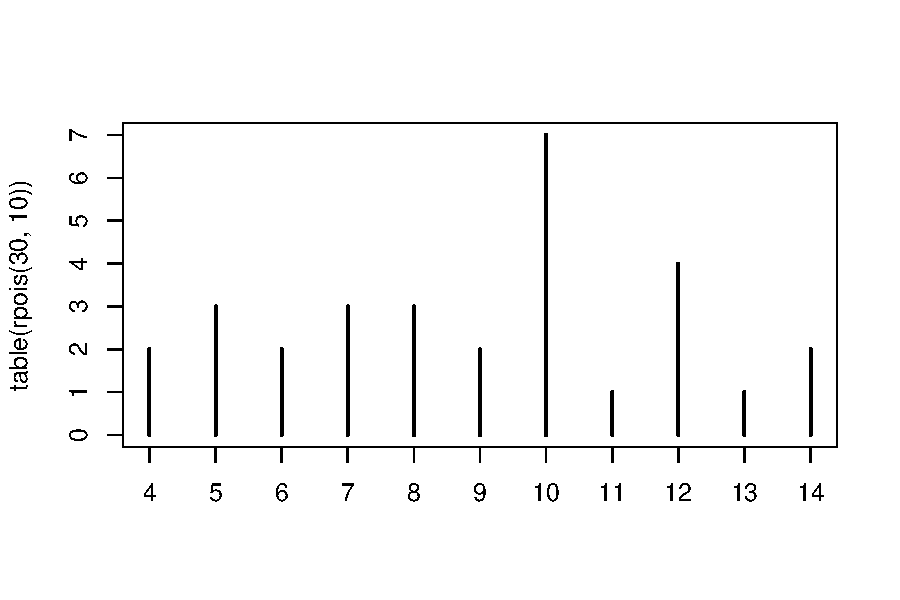
\includegraphics[keepaspectratio]{chapters/ch07_files/figure-pdf/unnamed-chunk-39-1.pdf}}

\subsection{\texorpdfstring{Contingency tables with
\texttt{ftable()}}{Contingency tables with ftable()}}\label{sec-summ-ftable}

\textbf{Contingency tables} summarize how many observations occur in
combinations of categories. They are calculated with \texttt{ftable()}.
This function counts the number of values in each combination of
different factors. The example below uses the built-in dataset
\texttt{iris} modified to have some additional factors.

\begin{Shaded}
\begin{Highlighting}[]
\FunctionTok{set.seed}\NormalTok{(}\DecValTok{123}\NormalTok{)}
\NormalTok{x }\OtherTok{\textless{}{-}}\NormalTok{ iris}
\NormalTok{x}\SpecialCharTok{$}\NormalTok{color }\OtherTok{\textless{}{-}} \FunctionTok{c}\NormalTok{(}\StringTok{"purple"}\NormalTok{, }\StringTok{"white"}\NormalTok{)}
\NormalTok{x}\SpecialCharTok{$}\NormalTok{bloom }\OtherTok{\textless{}{-}} \FunctionTok{sample}\NormalTok{(}\FunctionTok{c}\NormalTok{(}\StringTok{"early"}\NormalTok{, }\StringTok{"late"}\NormalTok{), }\FunctionTok{nrow}\NormalTok{(x), }\AttributeTok{replace=}\ConstantTok{TRUE}\NormalTok{)}
\NormalTok{color.ftab }\OtherTok{\textless{}{-}} \FunctionTok{ftable}\NormalTok{(x}\SpecialCharTok{$}\NormalTok{color}\SpecialCharTok{\textasciitilde{}}\NormalTok{x}\SpecialCharTok{$}\NormalTok{bloom)}
\NormalTok{color.ftab}
\end{Highlighting}
\end{Shaded}

\begin{verbatim}
        x$color purple white
x$bloom                     
early               39    37
late                36    38
\end{verbatim}

Contingency tables produced by \texttt{ftable()} can be used directly
for chi-squared (\(\chi^2\)) tests:

\begin{Shaded}
\begin{Highlighting}[]
\FunctionTok{chisq.test}\NormalTok{(color.ftab)}
\end{Highlighting}
\end{Shaded}

\begin{verbatim}

    Pearson's Chi-squared test with Yates' continuity correction

data:  color.ftab
X-squared = 0.026671, df = 1, p-value = 0.8703
\end{verbatim}

The function \texttt{ftable()} also has a formula interface, much like
many statistical functions (e.g., \texttt{lm()}) or
\texttt{aggregate()}. This is useful if you want more complicated tables
or more combinations of categories. Notice that the order of variables
affects the structure of the resulting table. The 6 commands below
produce equivalent tables, but the results are organized differently.

\begin{Shaded}
\begin{Highlighting}[]
\FunctionTok{ftable}\NormalTok{(Species}\SpecialCharTok{\textasciitilde{}}\NormalTok{color}\SpecialCharTok{+}\NormalTok{bloom, }\AttributeTok{data=}\NormalTok{x)}
\end{Highlighting}
\end{Shaded}

\begin{verbatim}
             Species setosa versicolor virginica
color  bloom                                    
purple early             17         13         9
       late               8         12        16
white  early             13         14        10
       late              12         11        15
\end{verbatim}

\begin{Shaded}
\begin{Highlighting}[]
\FunctionTok{ftable}\NormalTok{(Species}\SpecialCharTok{\textasciitilde{}}\NormalTok{color}\SpecialCharTok{+}\NormalTok{bloom, }\AttributeTok{data=}\NormalTok{x)}
\end{Highlighting}
\end{Shaded}

\begin{verbatim}
             Species setosa versicolor virginica
color  bloom                                    
purple early             17         13         9
       late               8         12        16
white  early             13         14        10
       late              12         11        15
\end{verbatim}

\begin{Shaded}
\begin{Highlighting}[]
\FunctionTok{ftable}\NormalTok{(Species}\SpecialCharTok{\textasciitilde{}}\NormalTok{bloom}\SpecialCharTok{+}\NormalTok{color, }\AttributeTok{data=}\NormalTok{x)}
\end{Highlighting}
\end{Shaded}

\begin{verbatim}
             Species setosa versicolor virginica
bloom color                                     
early purple             17         13         9
      white              13         14        10
late  purple              8         12        16
      white              12         11        15
\end{verbatim}

\begin{Shaded}
\begin{Highlighting}[]
\FunctionTok{ftable}\NormalTok{(color}\SpecialCharTok{\textasciitilde{}}\NormalTok{Species}\SpecialCharTok{+}\NormalTok{bloom, }\AttributeTok{data=}\NormalTok{x)}
\end{Highlighting}
\end{Shaded}

\begin{verbatim}
                 color purple white
Species    bloom                   
setosa     early           17    13
           late             8    12
versicolor early           13    14
           late            12    11
virginica  early            9    10
           late            16    15
\end{verbatim}

\begin{Shaded}
\begin{Highlighting}[]
\FunctionTok{ftable}\NormalTok{(color}\SpecialCharTok{\textasciitilde{}}\NormalTok{bloom}\SpecialCharTok{+}\NormalTok{Species, }\AttributeTok{data=}\NormalTok{x)}
\end{Highlighting}
\end{Shaded}

\begin{verbatim}
                 color purple white
bloom Species                      
early setosa               17    13
      versicolor           13    14
      virginica             9    10
late  setosa                8    12
      versicolor           12    11
      virginica            16    15
\end{verbatim}

\begin{Shaded}
\begin{Highlighting}[]
\FunctionTok{ftable}\NormalTok{(bloom}\SpecialCharTok{\textasciitilde{}}\NormalTok{color}\SpecialCharTok{+}\NormalTok{Species, }\AttributeTok{data=}\NormalTok{x)}
\end{Highlighting}
\end{Shaded}

\begin{verbatim}
                  bloom early late
color  Species                    
purple setosa              17    8
       versicolor          13   12
       virginica            9   16
white  setosa              13   12
       versicolor          14   11
       virginica           10   15
\end{verbatim}

\begin{Shaded}
\begin{Highlighting}[]
\FunctionTok{ftable}\NormalTok{(bloom}\SpecialCharTok{\textasciitilde{}}\NormalTok{Species}\SpecialCharTok{+}\NormalTok{color, }\AttributeTok{data=}\NormalTok{x)}
\end{Highlighting}
\end{Shaded}

\begin{verbatim}
                  bloom early late
Species    color                  
setosa     purple          17    8
           white           13   12
versicolor purple          13   12
           white           14   11
virginica  purple           9   16
           white           10   15
\end{verbatim}

Variables on the left side of the \texttt{\textasciitilde{}} will be on
the top of the table, and variables on the right side of the
\texttt{\textasciitilde{}} will be on the left side of the table. On
each side, variables are ordered in reverse order from the table matrix
outwards. I can never remember how this works, so usually just have to
tinker with the code until I get the table I want.

Compare the results of these commands:

\begin{Shaded}
\begin{Highlighting}[]
\FunctionTok{ftable}\NormalTok{(Species}\SpecialCharTok{\textasciitilde{}}\NormalTok{color}\SpecialCharTok{+}\NormalTok{bloom, }\AttributeTok{data=}\NormalTok{x)}
\end{Highlighting}
\end{Shaded}

\begin{verbatim}
             Species setosa versicolor virginica
color  bloom                                    
purple early             17         13         9
       late               8         12        16
white  early             13         14        10
       late              12         11        15
\end{verbatim}

\begin{Shaded}
\begin{Highlighting}[]
\FunctionTok{ftable}\NormalTok{(Species}\SpecialCharTok{\textasciitilde{}}\NormalTok{bloom}\SpecialCharTok{+}\NormalTok{color, }\AttributeTok{data=}\NormalTok{x)}
\end{Highlighting}
\end{Shaded}

\begin{verbatim}
             Species setosa versicolor virginica
bloom color                                     
early purple             17         13         9
      white              13         14        10
late  purple              8         12        16
      white              12         11        15
\end{verbatim}

The output of \texttt{ftable()} is of class \texttt{ftable}, which
\emph{looks} like a matrix or data frame but does not function like one.
Sometimes it is necessary to convert an \texttt{ftable()} output to
different class in order to pull values from it. This can be done with
base R conversion functions. Notice that the data frame form of
\texttt{handed.table} resembles the ``long'' data format we discussed in
Section~\ref{sec-manip-df-oth-shap}.

\begin{Shaded}
\begin{Highlighting}[]
\NormalTok{spp.color.ftab }\OtherTok{\textless{}{-}} \FunctionTok{ftable}\NormalTok{(x}\SpecialCharTok{$}\NormalTok{Species}\SpecialCharTok{\textasciitilde{}}\NormalTok{x}\SpecialCharTok{$}\NormalTok{color)}
\FunctionTok{as.matrix}\NormalTok{(spp.color.ftab)}
\end{Highlighting}
\end{Shaded}

\begin{verbatim}
        x$Species
x$color  setosa versicolor virginica
  purple     25         25        25
  white      25         25        25
\end{verbatim}

\begin{Shaded}
\begin{Highlighting}[]
\NormalTok{spp.color.df }\OtherTok{\textless{}{-}} \FunctionTok{as.data.frame}\NormalTok{(spp.color.ftab)}
\FunctionTok{names}\NormalTok{(spp.color.df) }\OtherTok{\textless{}{-}} \FunctionTok{c}\NormalTok{(}\StringTok{"color"}\NormalTok{, }\StringTok{"species"}\NormalTok{, }\StringTok{"freq"}\NormalTok{)}
\NormalTok{spp.color.df}
\end{Highlighting}
\end{Shaded}

\begin{verbatim}
   color    species freq
1 purple     setosa   25
2  white     setosa   25
3 purple versicolor   25
4  white versicolor   25
5 purple  virginica   25
6  white  virginica   25
\end{verbatim}

\chapter{Visualizing biological data}\label{sec-plot1}

\section{Visualizing single variables}\label{sec-plot1-single}

In statistics, we think of values within a variable coming from a
probability distribution. \textbf{Probability distributions}, or
\textbf{distributions} for short, are mathematical functions that
describe the way that values vary randomly. Distributions are a key idea
in statistics and data analysis and we'll cover them in detail in the
\href{@sec-dist}{next module}. We usually consider data to be
essentially random, but with the values forming predictable patterns
over many observations. The nature of those patterns is what probability
distributions attempt to model. A probability distribution does not tell
us the value of any particular observation, but it does let us estimate
the likelihood of observing any particular value. The figure below
demonstrates some common probability distributions: the heights of the
bars reflect the likelihood of the values on the \emph{x}-axes occurring
under those distributions.

\pandocbounded{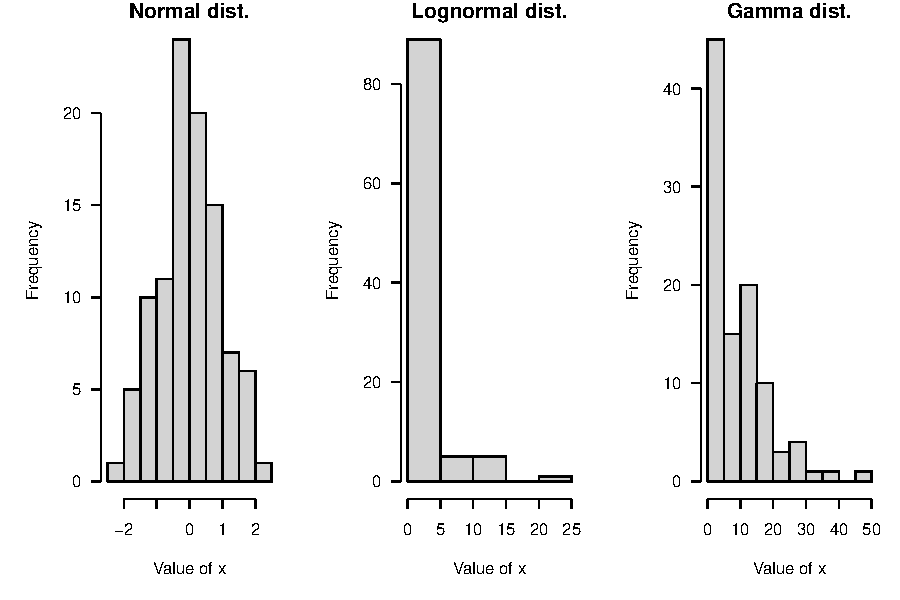
\includegraphics[keepaspectratio]{chapters/ch08_files/figure-pdf/unnamed-chunk-1-1.pdf}}

Successful data analysis requires paying attention to and thinking
carefully about the way that your data are distributed. Different kinds
of biological processes, like counts, waiting times, measurements, etc.,
have randomness that is described by different probability
distributions. The assumption that values follow certain distributions
is baked into most statistical methods. Trying to use a method that
assumes an inappropriate distribution will probably lead to invalid
results.

For example, if you try to analyze count data as if they came from a
continuous, unbounded distribution, your statistical model could predict
nonsensical outcomes such as negative or non-integer counts. The figure
below shows this: the red shaded area are predictions of negative
counts!

\pandocbounded{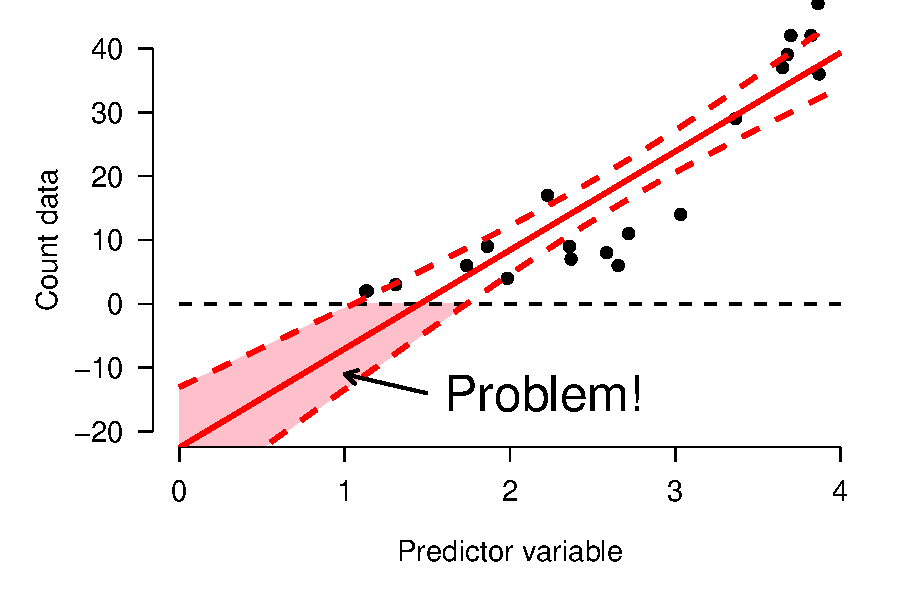
\includegraphics[keepaspectratio]{chapters/ch08_files/figure-pdf/unnamed-chunk-2-1.pdf}}

Sometimes it is not always obvious what distribution your data should
follow. Some cases are relatively straight forward: counts should
usually follow a Poisson or negative binomial distribution. Other cases
are less straightforward: should gene expression data be considered
normally, log-normally, or some other-ly distributed? Usually there is a
clear \emph{a priori} answer to this question that can be obtained by
thinking about what kind of process gave rise to the numbers.

A related question to ``what distribution does my data follow?'' is ``do
my data follow this distribution?'' Even if you have some expectation of
how your data should be distributed, that is no guarantee that your
study system cooperated. You should always check to see if your data
follow the distribution you assumed, and the distribution assumed by
your statistical test.

Deciding what distribution your data follow is always somewhat
subjective, and real datasets often contain some departure from
expectations. In this section we will explore some graphical techniques
and heuristics for determining how data are distributed.

Knowing about \href{@sec-dist}{data distributions} is a one thing, but
is quite another. Like much of the data analysis workflow, picking a
distribution can be as much an art as it is a science. This is because
distributions of real data are often messy, or do not conform exactly to
any one distribution, or may conform partly to several! Sometimes the
answer to ``what distribution should I use to analyze this data?'' is
not clear-cut.

The figure below gives a (very) rough guide to starting to identify a
response distribution. Note that this is only a guide for where to look
first, and not a definitive guide to selecting a response distribution.
Even if your choices lead you to, say, the normal distribution, you must
still verify that your data conform (at least roughly) to that
distribution. Note also that this diagram does not include every
distribution out there, but rather a select set of commonly encountered
distributions in biology.

\pandocbounded{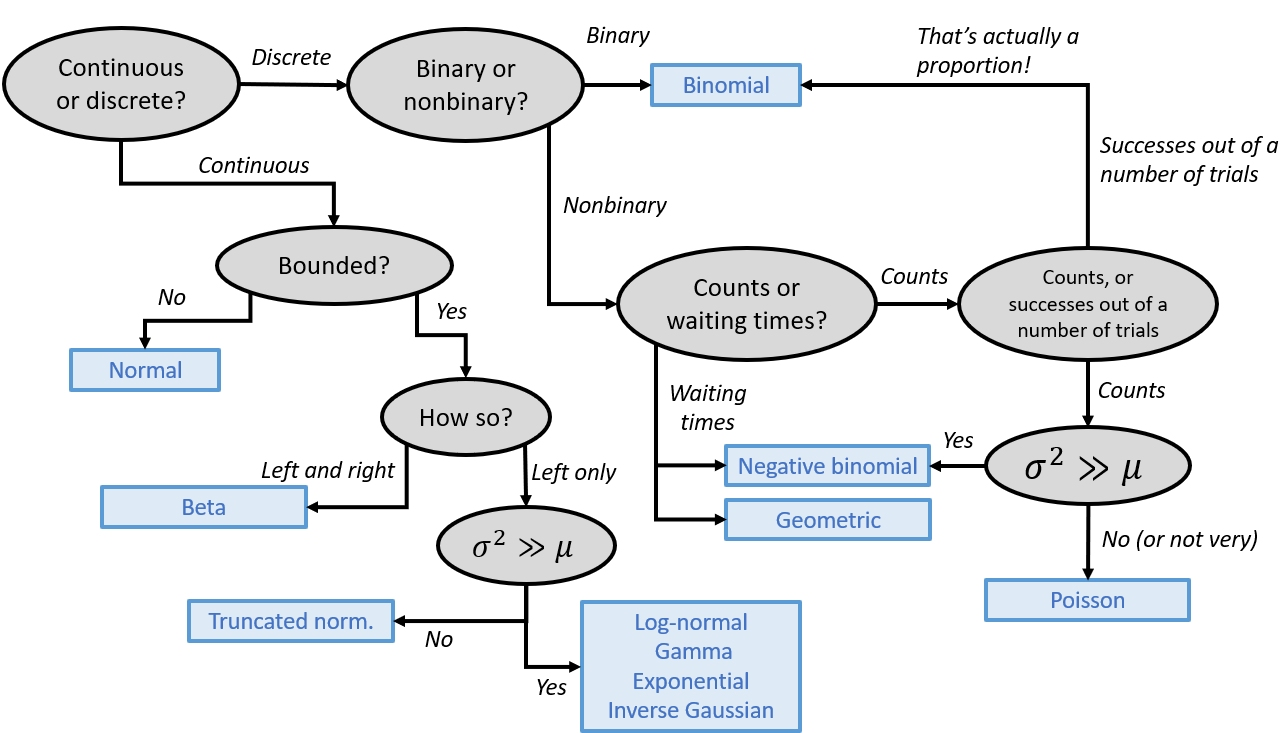
\includegraphics[keepaspectratio,alt={Flowchart for picking a probability distribution for your data}]{chapters/../images/08-01.jpg}}\{\#fig-alt=``Decision
tree for selecting a probability distribution based on the response
variable. First determine whether the response is continuous or
discrete. Continuous variables that are unbounded are modeled with a
normal distribution. Bounded continuous variables are modeled with a
beta distribution if bounded on both sides. If bounded only on the left,
use a truncated normal distribution when the variance is not much larger
than the mean, or a log-normal, gamma, exponential, or inverse Gaussian
distribution when the variance greatly exceeds the mean. For discrete
variables, first determine whether the response is binary. Binary
responses use a binomial distribution. Nonbinary discrete responses are
divided into counts and waiting times. Waiting times use a geometric
distribution or, when overdispersed, a negative binomial distribution.
Count data are next classified as simple counts or counts out of a fixed
denominator (proportions). Counts out of a denominator are treated as
binomial data. For simple counts, use a Poisson distribution when the
variance is approximately equal to the mean and a negative binomial
distribution when the variance greatly exceeds the mean.''\}

\subsection{Histograms}\label{sec-plot1-sing-hist}

\textbf{Histograms} show how values of a distribution are spread across
different intervals. These intervals are sometimes called \textbf{cells}
or \textbf{bins}. A good histogram will show, approximately, the shape
of a \textbf{probability density function (PDF)} of a
\href{@sec-dist-cont}{continuous distribution} or the
\textbf{probability mass function (PMF)} of a
\href{@sec-dist-disc}{discrete distribution}. A histogram with bin
widths of 0 should look like a \href{@sec-plot1-sing-kern}{kernel
density plot}.

The base function \texttt{hist()} will automatically select intervals
that look nice, but you can specify the intervals with argument
\texttt{breaks}.

\begin{Shaded}
\begin{Highlighting}[]
\NormalTok{x }\OtherTok{\textless{}{-}} \FunctionTok{rnorm}\NormalTok{(}\DecValTok{100}\NormalTok{)}

\CommentTok{\# 1 row, 2 column plot layout}
\FunctionTok{par}\NormalTok{(}\AttributeTok{mfrow=}\FunctionTok{c}\NormalTok{(}\DecValTok{1}\NormalTok{,}\DecValTok{2}\NormalTok{))}
\FunctionTok{hist}\NormalTok{(x, }\AttributeTok{sub=}\StringTok{"Default breaks"}\NormalTok{)}
\FunctionTok{hist}\NormalTok{(x, }\AttributeTok{breaks=}\FunctionTok{seq}\NormalTok{(}\SpecialCharTok{{-}}\DecValTok{4}\NormalTok{, }\DecValTok{4}\NormalTok{, }\AttributeTok{by=}\DecValTok{2}\NormalTok{), }\AttributeTok{sub=}\StringTok{"Different breaks"}\NormalTok{)}
\end{Highlighting}
\end{Shaded}

\pandocbounded{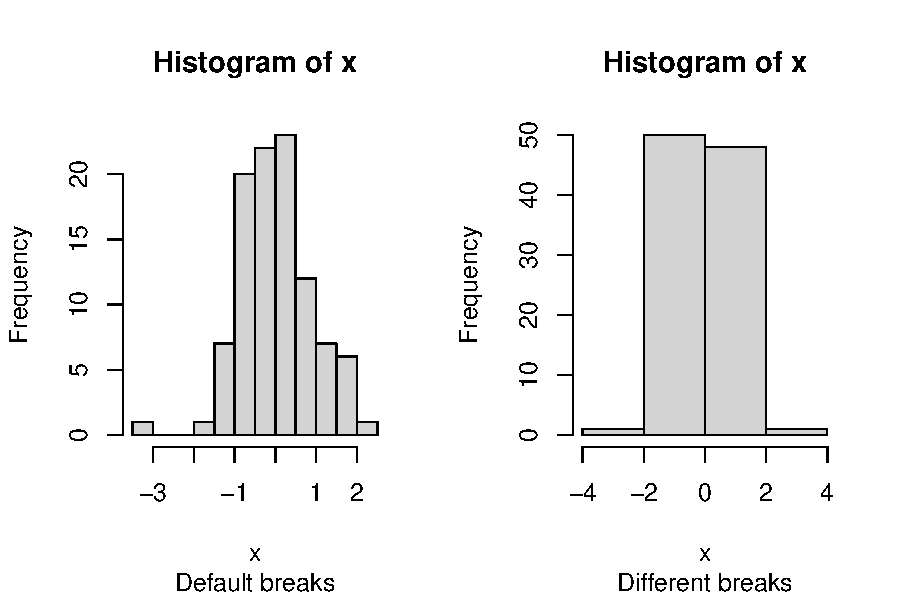
\includegraphics[keepaspectratio]{chapters/ch08_files/figure-pdf/unnamed-chunk-3-1.pdf}}

\begin{Shaded}
\begin{Highlighting}[]
\CommentTok{\# reset plot layout to 1 x 1}
\FunctionTok{par}\NormalTok{(}\AttributeTok{mfrow=}\FunctionTok{c}\NormalTok{(}\DecValTok{1}\NormalTok{,}\DecValTok{1}\NormalTok{))}
\end{Highlighting}
\end{Shaded}

The \emph{area} of each bar is also proportional to the number of values
in each interval.

R histograms can be presented as counts (\texttt{freq=TRUE}, the
default), or as probability density (\texttt{freq=FALSE}). We'll talk
more about probability density later in the
\href{@sec-manip-dists1}{next section}.

Compare these results:

\begin{Shaded}
\begin{Highlighting}[]
\FunctionTok{par}\NormalTok{(}\AttributeTok{mfrow=}\FunctionTok{c}\NormalTok{(}\DecValTok{1}\NormalTok{,}\DecValTok{2}\NormalTok{))}
\FunctionTok{hist}\NormalTok{(x)}
\FunctionTok{hist}\NormalTok{(x, }\AttributeTok{freq=}\ConstantTok{FALSE}\NormalTok{)}
\end{Highlighting}
\end{Shaded}

\pandocbounded{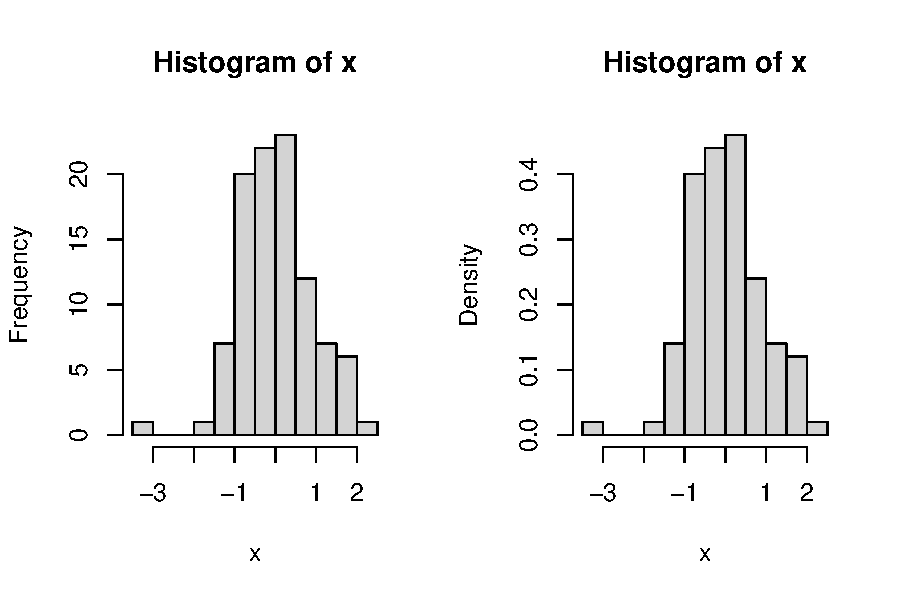
\includegraphics[keepaspectratio]{chapters/ch08_files/figure-pdf/unnamed-chunk-5-1.pdf}}

\begin{Shaded}
\begin{Highlighting}[]
\CommentTok{\# reset}
\FunctionTok{par}\NormalTok{(}\AttributeTok{mfrow=}\FunctionTok{c}\NormalTok{(}\DecValTok{1}\NormalTok{,}\DecValTok{1}\NormalTok{))}
\end{Highlighting}
\end{Shaded}

Because the second histogram shows probability densities, the areas
under the bars sum to 1 (this is part of the definition of a PDF) (see
Section~\ref{sec-dist-cont}).

A histogram can provide a visual first clue as to the shape of a
distribution's PDF or PMF. For example, the histograms of \texttt{x1}
and \texttt{x2} below suggest very different distributions:

\begin{Shaded}
\begin{Highlighting}[]
\NormalTok{x1 }\OtherTok{\textless{}{-}} \FunctionTok{rnorm}\NormalTok{(}\DecValTok{1000}\NormalTok{)}
\NormalTok{x2 }\OtherTok{\textless{}{-}} \FunctionTok{rlnorm}\NormalTok{(}\DecValTok{1000}\NormalTok{)}

\FunctionTok{par}\NormalTok{(}\AttributeTok{mfrow=}\FunctionTok{c}\NormalTok{(}\DecValTok{1}\NormalTok{,}\DecValTok{2}\NormalTok{))}
\FunctionTok{hist}\NormalTok{(x1)}
\FunctionTok{hist}\NormalTok{(x2)}
\end{Highlighting}
\end{Shaded}

\pandocbounded{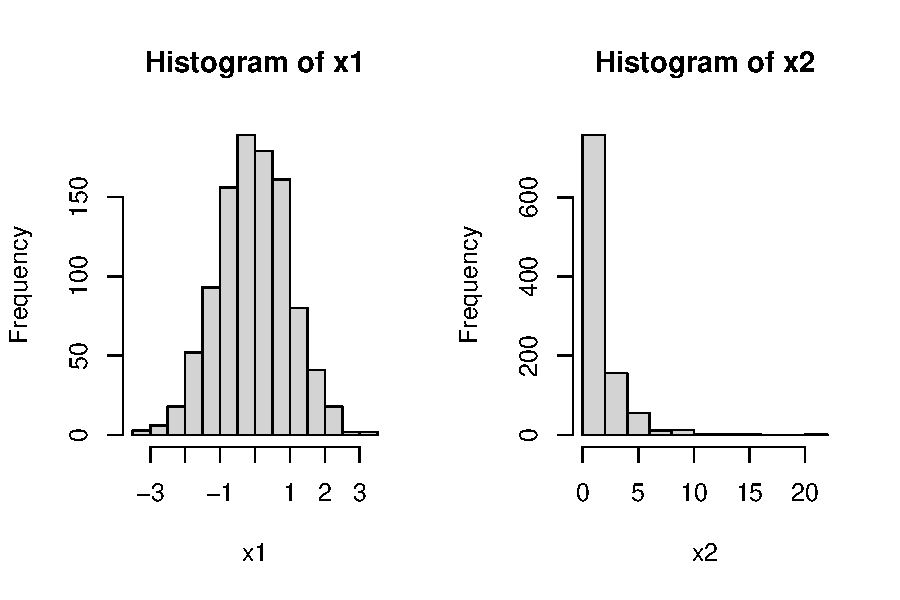
\includegraphics[keepaspectratio]{chapters/ch08_files/figure-pdf/unnamed-chunk-6-1.pdf}}

\begin{Shaded}
\begin{Highlighting}[]
\CommentTok{\# reset}
\FunctionTok{par}\NormalTok{(}\AttributeTok{mfrow=}\FunctionTok{c}\NormalTok{(}\DecValTok{1}\NormalTok{,}\DecValTok{1}\NormalTok{))}
\end{Highlighting}
\end{Shaded}

Notice that \texttt{x1} appears roughly normal. It is symmetric, has a
bell-shape, and is concentrated near its center. Contrast this with
\texttt{x2}. Distribution \texttt{x2} is strongly right-skewed (i.e.,
lots of small values with a long positive tail), with most values near
0. It also has no negative values (\texttt{range(x2)}). Because of these
properties we might suspect that \texttt{x2} is really a log-normal
distribution. We can check this by making a histogram of the log of
\texttt{x2}:

\begin{Shaded}
\begin{Highlighting}[]
\FunctionTok{hist}\NormalTok{(}\FunctionTok{log}\NormalTok{(x2))}
\end{Highlighting}
\end{Shaded}

\pandocbounded{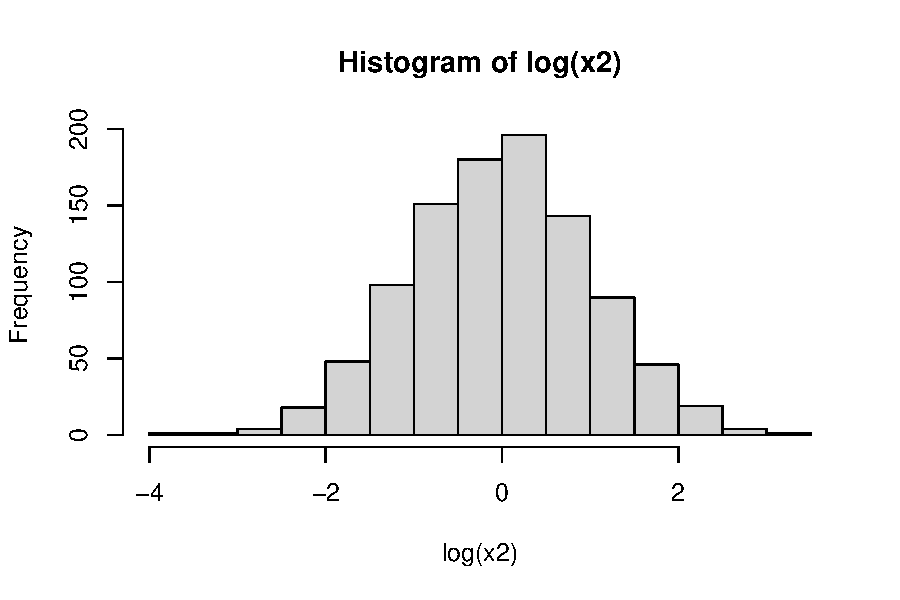
\includegraphics[keepaspectratio]{chapters/ch08_files/figure-pdf/unnamed-chunk-7-1.pdf}}

Other distributions might be tricky. Consider the histograms below:

\begin{Shaded}
\begin{Highlighting}[]
\NormalTok{x1 }\OtherTok{\textless{}{-}} \FunctionTok{rnorm}\NormalTok{(}\DecValTok{1000}\NormalTok{, }\DecValTok{5}\NormalTok{, }\DecValTok{2}\NormalTok{)}
\NormalTok{x2 }\OtherTok{\textless{}{-}} \FunctionTok{rnorm}\NormalTok{(}\DecValTok{1000}\NormalTok{, }\DecValTok{15}\NormalTok{, }\DecValTok{3}\NormalTok{)}
\NormalTok{x3 }\OtherTok{\textless{}{-}} \FunctionTok{c}\NormalTok{(x1, x2)}

\NormalTok{x1 }\OtherTok{\textless{}{-}} \FunctionTok{rnorm}\NormalTok{(}\DecValTok{1000}\NormalTok{, }\DecValTok{5}\NormalTok{, }\DecValTok{2}\NormalTok{)}
\NormalTok{x2 }\OtherTok{\textless{}{-}} \FunctionTok{runif}\NormalTok{(}\DecValTok{1000}\NormalTok{, }\DecValTok{3}\NormalTok{, }\DecValTok{20}\NormalTok{)}
\NormalTok{x4 }\OtherTok{\textless{}{-}} \FunctionTok{c}\NormalTok{(x1, x2)}

\FunctionTok{par}\NormalTok{(}\AttributeTok{mfrow=}\FunctionTok{c}\NormalTok{(}\DecValTok{1}\NormalTok{,}\DecValTok{2}\NormalTok{))}
\FunctionTok{hist}\NormalTok{(x3)}
\FunctionTok{hist}\NormalTok{(x4)}
\end{Highlighting}
\end{Shaded}

\pandocbounded{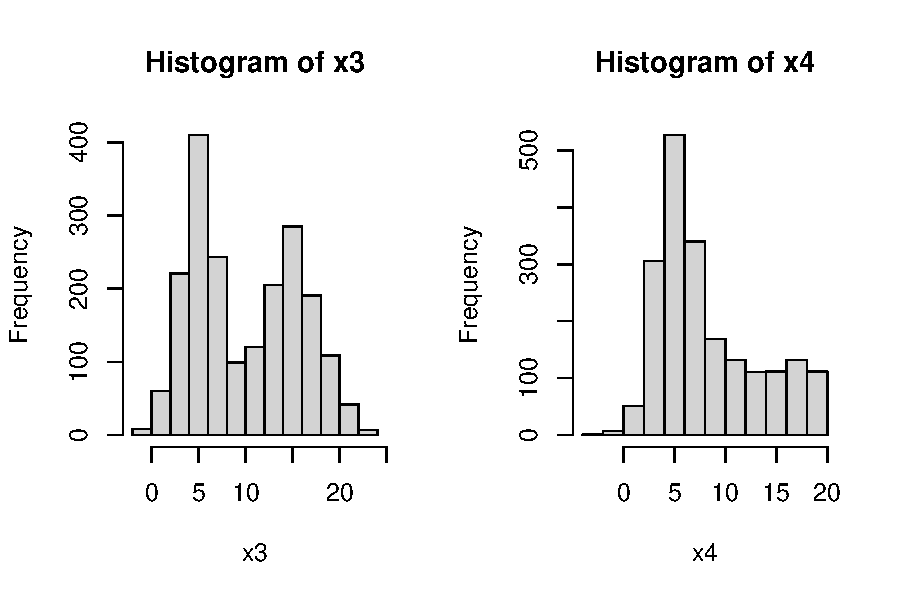
\includegraphics[keepaspectratio]{chapters/ch08_files/figure-pdf/unnamed-chunk-8-1.pdf}}

\begin{Shaded}
\begin{Highlighting}[]
\CommentTok{\# reset}
\FunctionTok{par}\NormalTok{(}\AttributeTok{mfrow=}\FunctionTok{c}\NormalTok{(}\DecValTok{1}\NormalTok{,}\DecValTok{1}\NormalTok{))}
\end{Highlighting}
\end{Shaded}

What a mess!

\begin{itemize}
\tightlist
\item
  Histogram \texttt{x3} shows what is commonly referred to as a
  \textbf{bimodal} distribution. This is a distribution with two
  \textbf{modes}, or most common values, with a gap between them.
  Bimodal distributions often arise from a \textbf{mixture} of two
  distributions (in this case, two normals). Or, they can indicate that
  something in the data generating process leads to diverging outcomes.
  For example, in many college courses the grade distribution can be
  bimodal, with most students making either a B or D.
\item
  Histogram \texttt{x4} shows a distribution with some right skew, but
  not the long, tapering tail characteristic of the lognormal
  distribution (see \texttt{x2}, above). The fact that the mean is near
  5 and not 0 is another point against a lognormal. But the clincher is
  that there are negative values, which a lognormal distribution cannot
  take (think about why this is).
\end{itemize}

Think for a few minutes about what distribution \texttt{x4} might be,
then click the footnote to find out\footnote{Distribution \texttt{x4} is
  a mixture of a normal with mean = 5 and SD = 2 with a uniform in {[}3,
  20{]}.}.

\subsection{Barplots}\label{sec-plot1-sing-bar}

Barplots are usually used to show the \emph{mean} within each group.
But, that's all they show. Barplots might be more appropriate than
barplots if you have so many groups that a boxplot is too cluttered to
read, or if the distributions within each group are known to be
symmetrical and about the same width (and thus, showing them is not
necessary).

Unlike \texttt{boxplot()}, \texttt{barplot()} does not calculate its own
values. The values supplied to \texttt{barplot()} will be used as the
bar heights. This means you need to calculate the means (or medians or
whatever) ahead of time using a function like \texttt{aggregate()}. In
the example, below, SD is also calculated so the plot will include some
measure of variability. This is one of the disadvantages of barplots in
R compared to boxplots: \texttt{boxplot()} automatically computes and
displays variability about the mean, but \texttt{barplot()} does not.

Another difference is that unlike \texttt{boxplot()}, the \emph{x}
coordinates in a barplot are calculated by the \texttt{barplot()}
function. What this means is that you often need to run it twice: once
to get the \emph{x} coordinates, and again to make the plot. Those
\emph{x} coordinates are needed to place the line segments that show the
SD.

\begin{Shaded}
\begin{Highlighting}[]
\CommentTok{\# get means and SD of a y variable by species in iris}
\NormalTok{agg }\OtherTok{\textless{}{-}} \FunctionTok{aggregate}\NormalTok{(Petal.Length}\SpecialCharTok{\textasciitilde{}}\NormalTok{Species, }\AttributeTok{data=}\NormalTok{iris, mean)}
\NormalTok{agg}\SpecialCharTok{$}\NormalTok{sd }\OtherTok{\textless{}{-}} \FunctionTok{aggregate}\NormalTok{(Petal.Length}\SpecialCharTok{\textasciitilde{}}\NormalTok{Species,}
                    \AttributeTok{data=}\NormalTok{iris, sd)}\SpecialCharTok{$}\NormalTok{Petal.Length}

\CommentTok{\# get x axis values}
\NormalTok{bar }\OtherTok{\textless{}{-}} \FunctionTok{barplot}\NormalTok{(Petal.Length}\SpecialCharTok{\textasciitilde{}}\NormalTok{Species, }\AttributeTok{data=}\NormalTok{agg)}
\end{Highlighting}
\end{Shaded}

\begin{center}
\pandocbounded{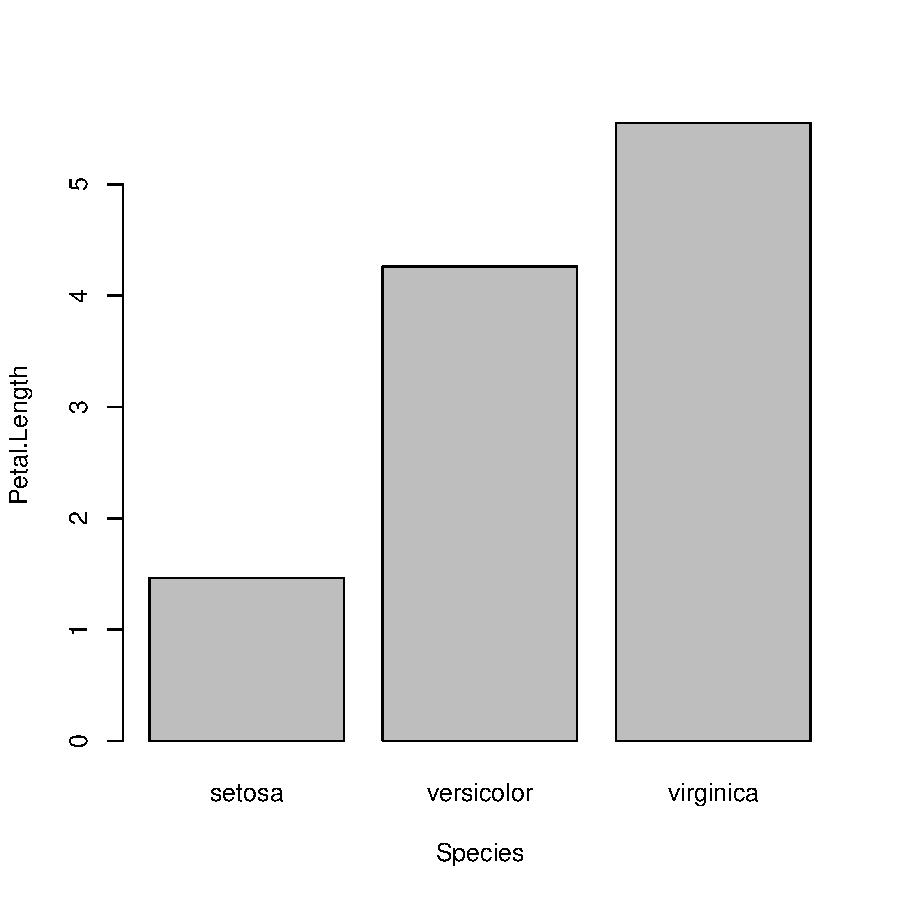
\includegraphics[keepaspectratio]{chapters/ch08_files/figure-pdf/unnamed-chunk-9-1.pdf}}
\end{center}

\begin{Shaded}
\begin{Highlighting}[]
\CommentTok{\# make plot with second call}
\FunctionTok{barplot}\NormalTok{(Petal.Length}\SpecialCharTok{\textasciitilde{}}\NormalTok{Species, }\AttributeTok{data=}\NormalTok{agg, }\AttributeTok{ylim=}\FunctionTok{c}\NormalTok{(}\DecValTok{0}\NormalTok{, }\DecValTok{7}\NormalTok{))}
\FunctionTok{segments}\NormalTok{(bar[,}\DecValTok{1}\NormalTok{], agg}\SpecialCharTok{$}\NormalTok{Petal.Length, bar[,}\DecValTok{1}\NormalTok{], agg}\SpecialCharTok{$}\NormalTok{Petal.Length}\SpecialCharTok{+}\NormalTok{agg}\SpecialCharTok{$}\NormalTok{sd)}
\end{Highlighting}
\end{Shaded}

\pandocbounded{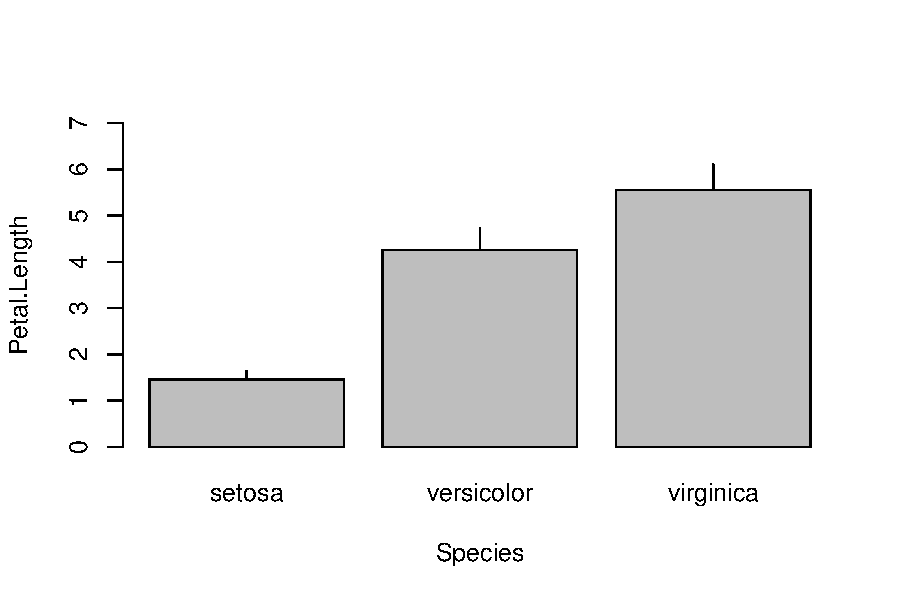
\includegraphics[keepaspectratio]{chapters/ch08_files/figure-pdf/unnamed-chunk-10-1.pdf}}

The above plot is called a ``dynamite plot'' because the bar and error
bar look like an old stick of dynamite. Because they show less than a
boxplot, and are harder to make than a boxplot, I almost never make
dynamite plots. Instead, I suggest you use boxplots or something like
the ``point-and-whisker'' plots below
(Section~\ref{sec-plot1-sing-box}).

\subsection{Boxplots}\label{sec-plot1-sing-box}

\textbf{Boxplots}, or \textbf{box-and-whisker plots}, summarize the
distribution of continuous variables. They are often used to summarize
data by a factor, making it easier to see how the distribution of a
variable differs between groups. The boxplot shows the median, the first
and third quartiles, and extreme values (whiskers and
points)\footnote{Or close enough. The actual, slightly different values,
  are in the documentation. See \texttt{?boxplot.stats}.}.

Boxplot of a single variable:

\begin{Shaded}
\begin{Highlighting}[]
\FunctionTok{boxplot}\NormalTok{(iris}\SpecialCharTok{$}\NormalTok{Petal.Width)}
\end{Highlighting}
\end{Shaded}

\pandocbounded{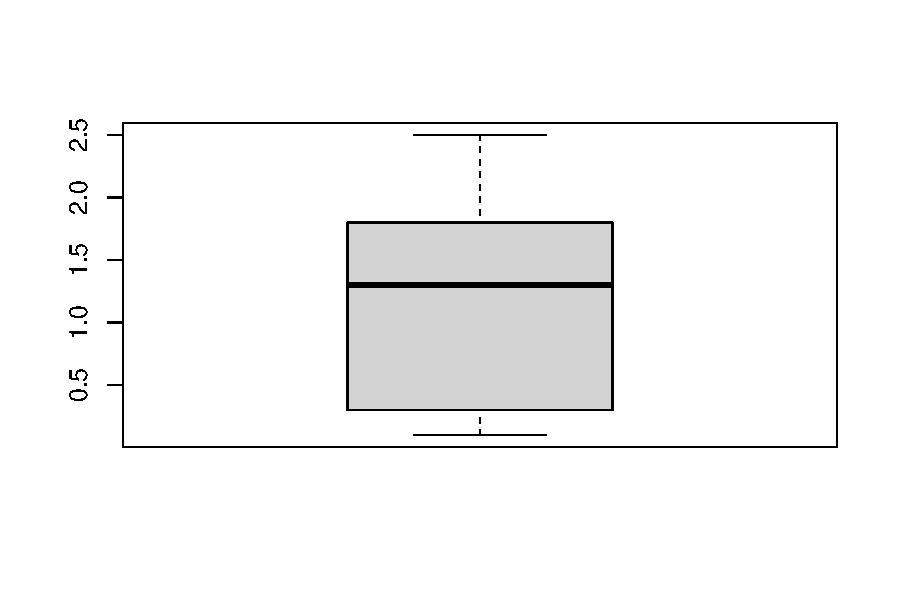
\includegraphics[keepaspectratio]{chapters/ch08_files/figure-pdf/unnamed-chunk-11-1.pdf}}

Boxplot with some options for a nicer plot:

\begin{Shaded}
\begin{Highlighting}[]
\FunctionTok{boxplot}\NormalTok{(iris}\SpecialCharTok{$}\NormalTok{Petal.Width,}
        \AttributeTok{ylab=}\StringTok{"Petal width (cm)"}\NormalTok{,}
        \AttributeTok{ylim=}\FunctionTok{c}\NormalTok{(}\DecValTok{0}\NormalTok{,}\DecValTok{3}\NormalTok{))}
\end{Highlighting}
\end{Shaded}

\pandocbounded{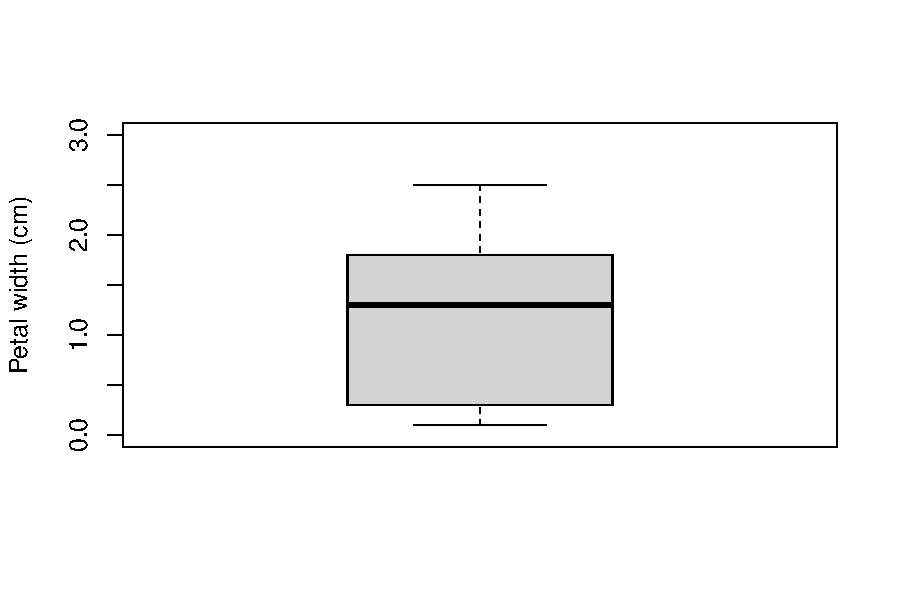
\includegraphics[keepaspectratio]{chapters/ch08_files/figure-pdf/unnamed-chunk-12-1.pdf}}

Boxplot across levels of a factor (note formula interface):

\begin{Shaded}
\begin{Highlighting}[]
\FunctionTok{boxplot}\NormalTok{(iris}\SpecialCharTok{$}\NormalTok{Petal.Width}\SpecialCharTok{\textasciitilde{}}\NormalTok{iris}\SpecialCharTok{$}\NormalTok{Species,}
        \AttributeTok{xlab=}\StringTok{"Species"}\NormalTok{,}
        \AttributeTok{ylab=}\StringTok{"Petal.Width (cm)"}\NormalTok{,}
        \AttributeTok{ylim=}\FunctionTok{c}\NormalTok{(}\DecValTok{0}\NormalTok{,}\DecValTok{3}\NormalTok{))}
\end{Highlighting}
\end{Shaded}

\pandocbounded{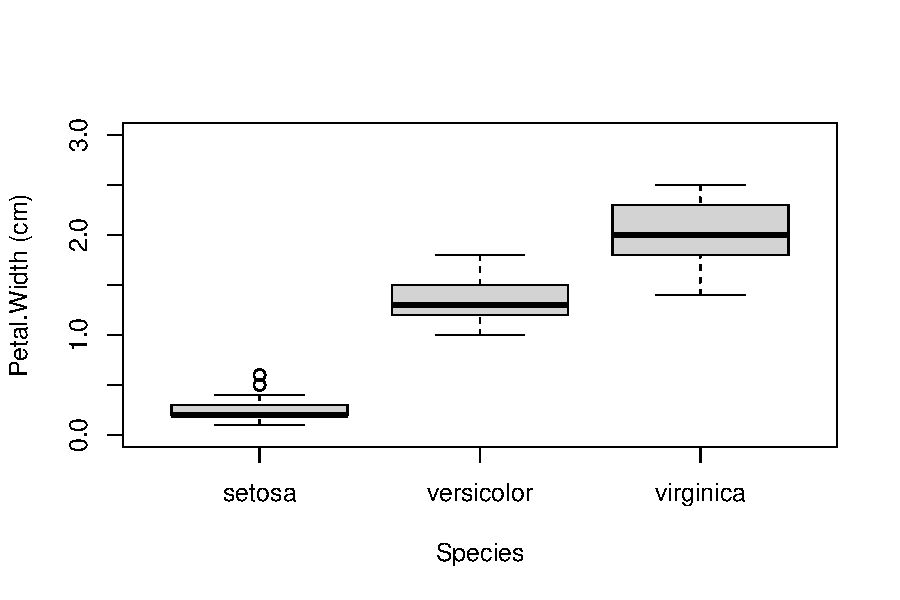
\includegraphics[keepaspectratio]{chapters/ch08_files/figure-pdf/unnamed-chunk-13-1.pdf}}

A highly asymmetric box-and-whisker plot can indicate that data are
skewed or non-normal.

The base \texttt{boxplot()} function can produce summaries across
multiple variables. Essentially it treats each combination of grouping
variables as a separate set of values. There are better ways to plot
group differences (e.g., for publication), but the base
\texttt{boxplot()} does just fine for data exploration.

Boxplots can be constructed using several grouping variables. The order
of grouping variables in the formula will determine the order of boxes
in the plot.

\begin{Shaded}
\begin{Highlighting}[]
\NormalTok{x }\OtherTok{\textless{}{-}}\NormalTok{ iris}
\NormalTok{x}\SpecialCharTok{$}\NormalTok{color }\OtherTok{\textless{}{-}} \FunctionTok{c}\NormalTok{(}\StringTok{"red"}\NormalTok{, }\StringTok{"white"}\NormalTok{) }\CommentTok{\#made up variable}

\CommentTok{\# group by species and color:}
\FunctionTok{boxplot}\NormalTok{(Petal.Width}\SpecialCharTok{\textasciitilde{}}\NormalTok{Species}\SpecialCharTok{+}\NormalTok{color, }\AttributeTok{data=}\NormalTok{x,}
        \AttributeTok{ylab=}\StringTok{"Petal width (cm)"}\NormalTok{, }\AttributeTok{ylim=}\FunctionTok{c}\NormalTok{(}\DecValTok{0}\NormalTok{,}\DecValTok{3}\NormalTok{))}
\end{Highlighting}
\end{Shaded}

\pandocbounded{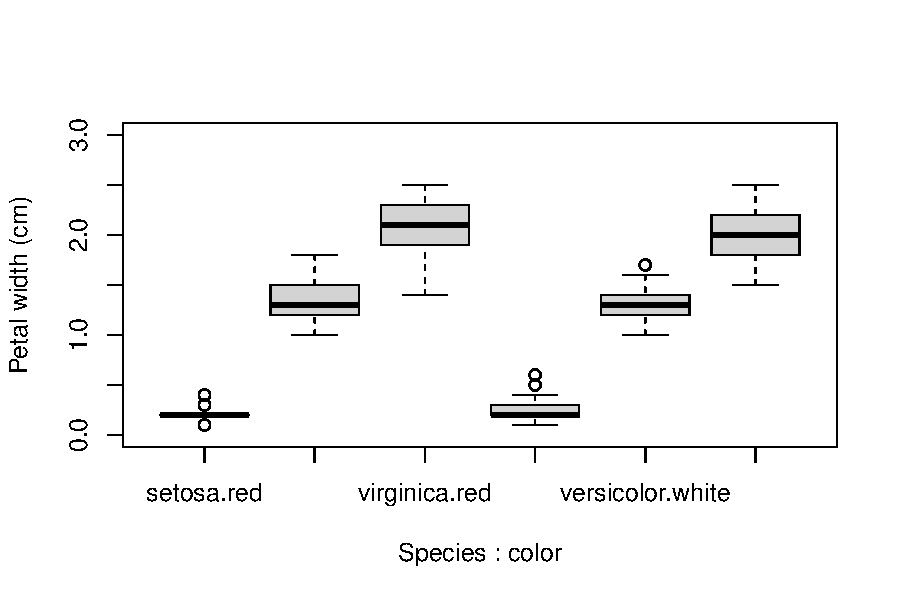
\includegraphics[keepaspectratio]{chapters/ch08_files/figure-pdf/unnamed-chunk-14-1.pdf}}

Notice the difference in order of grouping:

\begin{Shaded}
\begin{Highlighting}[]
\CommentTok{\# difference in order of grouping:}
\FunctionTok{boxplot}\NormalTok{(Petal.Width}\SpecialCharTok{\textasciitilde{}}\NormalTok{color}\SpecialCharTok{+}\NormalTok{Species, }\AttributeTok{data=}\NormalTok{x,}
        \AttributeTok{ylab=}\StringTok{"Petal width (cm)"}\NormalTok{, }\AttributeTok{ylim=}\FunctionTok{c}\NormalTok{(}\DecValTok{0}\NormalTok{,}\DecValTok{3}\NormalTok{))}
\end{Highlighting}
\end{Shaded}

\pandocbounded{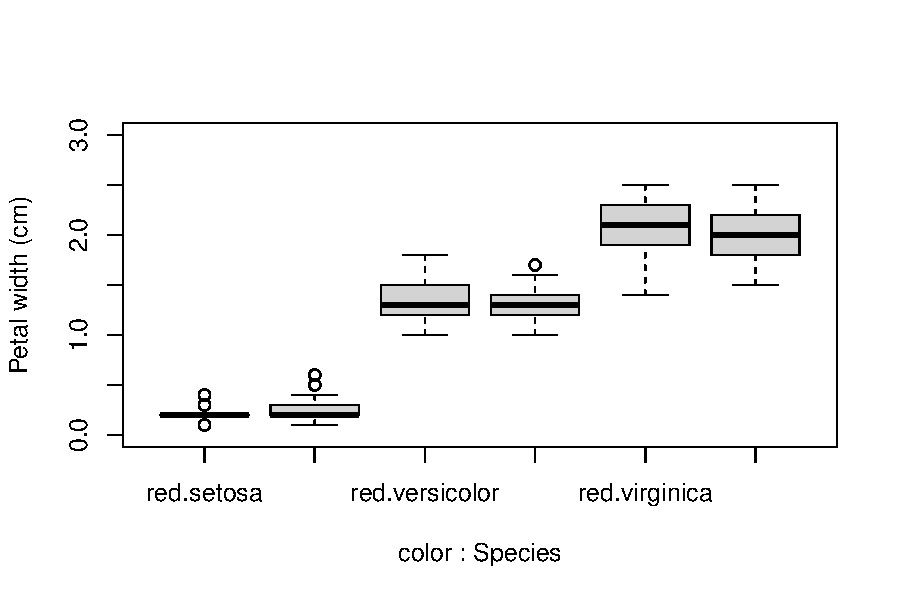
\includegraphics[keepaspectratio]{chapters/ch08_files/figure-pdf/unnamed-chunk-15-1.pdf}}

When constructing complicated boxplots, you may need to manually fix the
x-axis labels, because they are not all rendered. Fortunately, the
x-axis tick marks are simply numbered from left to right. So if, say,
the 6\textsuperscript{th} label was missing, you can draw it manually
like this:

\begin{Shaded}
\begin{Highlighting}[]
\FunctionTok{boxplot}\NormalTok{(Petal.Width}\SpecialCharTok{\textasciitilde{}}\NormalTok{Species}\SpecialCharTok{+}\NormalTok{color, }\AttributeTok{data=}\NormalTok{x,}
        \AttributeTok{ylab=}\StringTok{"Petal width (cm)"}\NormalTok{, }\AttributeTok{ylim=}\FunctionTok{c}\NormalTok{(}\DecValTok{0}\NormalTok{,}\DecValTok{3}\NormalTok{))}
\CommentTok{\# add missing tick mark with axis()}
\FunctionTok{axis}\NormalTok{(}\AttributeTok{side=}\DecValTok{1}\NormalTok{, }\AttributeTok{at=}\DecValTok{6}\NormalTok{, }\AttributeTok{labels=}\StringTok{"virginica.white"}\NormalTok{)}
\end{Highlighting}
\end{Shaded}

\pandocbounded{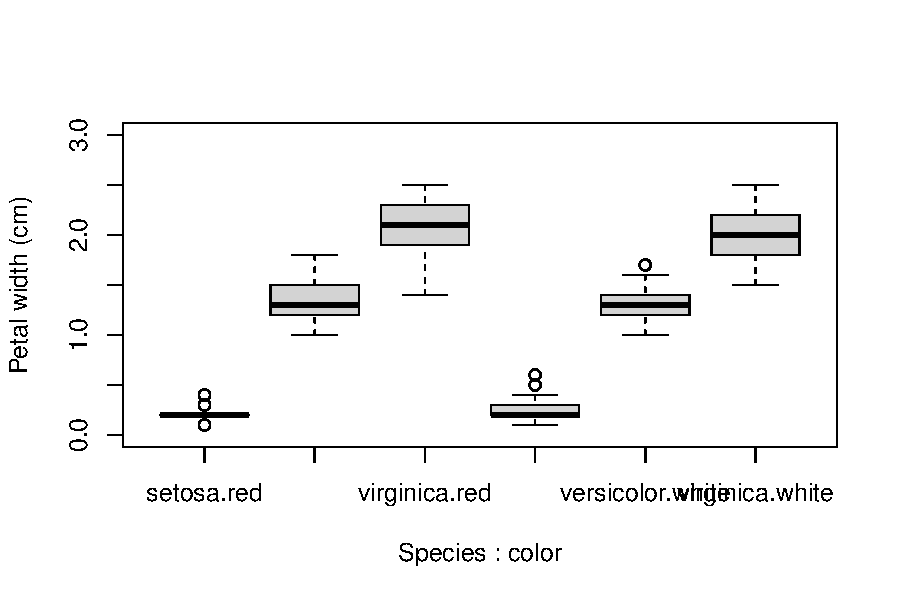
\includegraphics[keepaspectratio]{chapters/ch08_files/figure-pdf/unnamed-chunk-16-1.pdf}}

If you want to construct a totally custom box and whisker plot, you can
do so using base graphics functions like \texttt{rect()},
\texttt{arrows()}, \texttt{segments()}, and so on. All you need is to
get the values for the different parts of the boxplot by saving a
boxplot to an object.

\begin{Shaded}
\begin{Highlighting}[]
\CommentTok{\# not run}
\NormalTok{myboxplot }\OtherTok{\textless{}{-}} \FunctionTok{boxplot}\NormalTok{(Petal.Width}\SpecialCharTok{\textasciitilde{}}\NormalTok{Species}\SpecialCharTok{+}\NormalTok{color, }\AttributeTok{data=}\NormalTok{x)}
\end{Highlighting}
\end{Shaded}

The \texttt{stats} part of the resulting list will contain most of what
you need. See \texttt{?boxplot.stats} for a guide.

\subsection{ECDF plots}\label{sec-plot1-sing-cdf}

The \textbf{cumulative distribution function (CDF)} is the probability
that a random variable will take on a value less than or equal to some
value. Formally, we say that a continuous distribution \(x\) will take
on value \(\le{x}\) with probability \(F\left(x\right)\), where
\(F\left(x\right)\) is the CDF.

The figure below shows what this means.

\pandocbounded{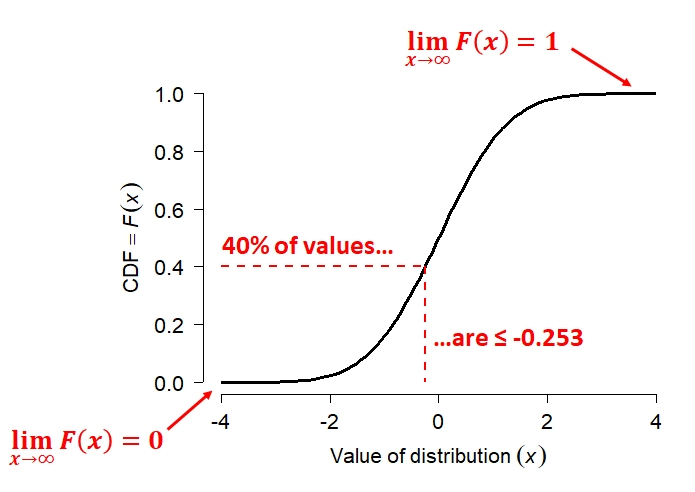
\includegraphics[keepaspectratio,alt={Relationship between the cumulative distribution function (CDF, quantiles, and values of a variable x. The CDF, F(x), gives the probability that a random variable is less than or equal to a specified value. In this example, F(−0.253)=0.4, meaning that 40\% of observations are expected to be less than or equal to −0.253. The CDF approaches 0 as x \textbackslash rightarrow -\textbackslash infty and 1 as x \textbackslash rightarrow +\textbackslash infty.}]{chapters/../images/08-03.jpg}}\{alt-text:
``Plot of the cumulative distribution function (CDF) of a normal
distribution. The CDF is an S-shaped curve that increases smoothly from
0 to 1 as the value of the variable increases. Dashed red lines
highlight the point where the CDF equals 0.4, showing that 40\% of
observations are less than or equal to x=−0.253. Additional annotations
indicate that the CDF approaches 0 for very small values of x and
approaches 1 for very large values of x. The figure illustrates that the
CDF gives the cumulative probability up to a specified value of the
variable.''\}

The figure shows the CDF of a normal distribution with mean = 0 and SD =
1 (i.e., the standard normal distribution. Like all CDFs,
\(F\left(x\right)\) increases monotonically (slope never changing sign)
from 0 to 1 as \(x\) increases from the lower bound to the upper bound
of the distribution.

In the case of the normal distribution, the bounds of \(x\) are
\(\left[-\infty,+\infty\right]\). The CDF approaches 0 as \(x\)
decreases, and approaches 1 as \(x\) increases.

The red dashed lines show how to interpret the relationship between the
axes. For any value on the \emph{x}-axis, the \emph{y}-axis shows what
proportion of values are \(\le{x}\). For any value on the \emph{y}-axis,
the \emph{x}-axis shows the value at the \emph{y}-th quantile of the
distribution.

\textbf{The CDF is in a very real sense the \emph{definition} of a
probability distribution.}

Every probability distribution can be identified by a unique CDF. It
doesn't matter whether a distribution is continuous, discrete, or a
mixture of both. The figure below shows what the CDFs of a discrete or
mixed distribution look like compared to that of a continuous
distribution\footnote{adapted from
  \url{https://commons.wikimedia.org/wiki/File:Discrete_probability_distribution_illustration.svg}
  (public domain).}.

\pandocbounded{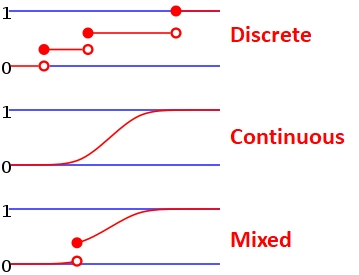
\includegraphics[keepaspectratio,alt={Examples of cumulative distribution functions for different types of random variables. Discrete variables have stepwise CDFs because probability accumulates only at specific values. Continuous variables have smooth CDFs because probability accumulates continuously over an interval. Mixed distributions combine both features, with smooth segments interrupted by jumps corresponding to point masses.}]{chapters/../images/08-04.jpg}}\{Three
schematic cumulative distribution functions (CDFs) illustrating
different types of distributions. The top panel, labeled ``Discrete,''
shows a step function with horizontal segments and jumps; open circles
indicate the CDF immediately before each jump and filled circles
indicate the value after the jump. The middle panel, labeled
``Continuous,'' shows a smooth S-shaped curve with no jumps, indicating
that the CDF changes continuously. The bottom panel, labeled ``Mixed,''
shows a smooth curve containing a single jump, illustrating a
distribution with both continuous probability and discrete point masses.
The figure emphasizes that CDFs are step functions for discrete
variables, smooth for continuous variables, and a combination of both
for mixed distributions.\}

The examples below calculate and plot ECDF plots for a uniform (left)
and a normal distribution (right).

\begin{Shaded}
\begin{Highlighting}[]
\FunctionTok{set.seed}\NormalTok{(}\DecValTok{42}\NormalTok{)}
\NormalTok{n }\OtherTok{\textless{}{-}} \FloatTok{1e3}
\NormalTok{x1 }\OtherTok{\textless{}{-}} \FunctionTok{runif}\NormalTok{(n, }\DecValTok{3}\NormalTok{, }\DecValTok{8}\NormalTok{)}
\NormalTok{x2 }\OtherTok{\textless{}{-}} \FunctionTok{rnorm}\NormalTok{(n, }\DecValTok{7}\NormalTok{, }\DecValTok{4}\NormalTok{)}
\FunctionTok{par}\NormalTok{(}\AttributeTok{mfrow=}\FunctionTok{c}\NormalTok{(}\DecValTok{1}\NormalTok{,}\DecValTok{2}\NormalTok{))}
\FunctionTok{plot}\NormalTok{(}\FunctionTok{ecdf}\NormalTok{(x1))}
\FunctionTok{plot}\NormalTok{(}\FunctionTok{ecdf}\NormalTok{(x2))}
\CommentTok{\# add lines at 20th percentile:}
\FunctionTok{abline}\NormalTok{(}\AttributeTok{h=}\FloatTok{0.2}\NormalTok{, }\AttributeTok{lty=}\DecValTok{2}\NormalTok{, }\AttributeTok{col=}\StringTok{"red"}\NormalTok{)}
\FunctionTok{abline}\NormalTok{(}\AttributeTok{v=}\FunctionTok{quantile}\NormalTok{(x2, }\FloatTok{0.2}\NormalTok{), }\AttributeTok{lty=}\DecValTok{2}\NormalTok{, }\AttributeTok{col=}\StringTok{"red"}\NormalTok{)}
\end{Highlighting}
\end{Shaded}

\begin{center}
\pandocbounded{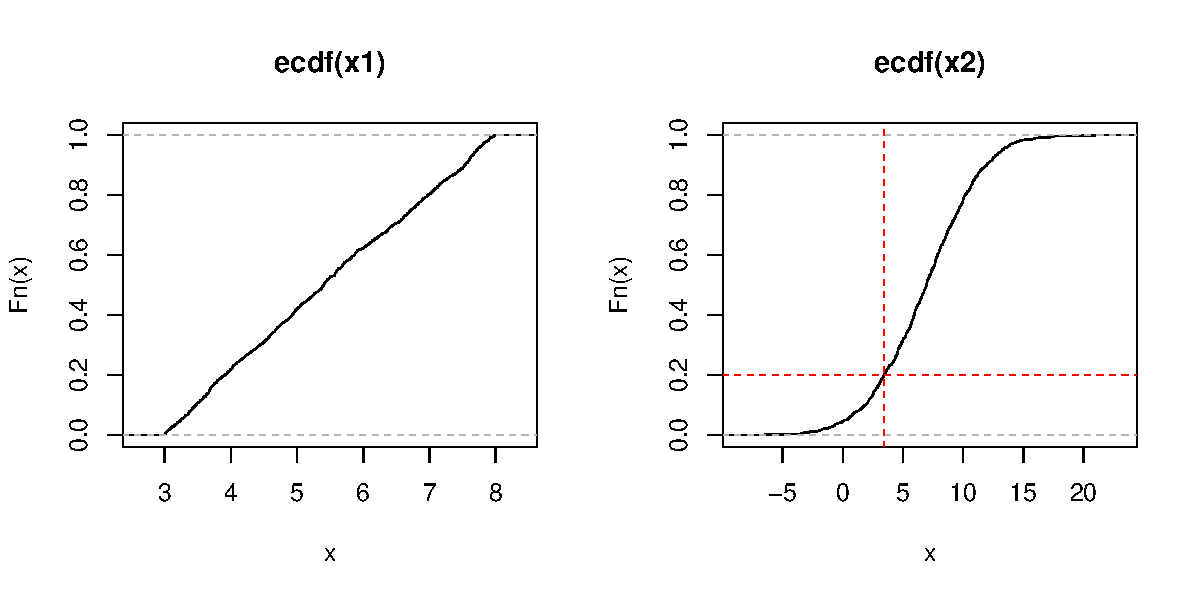
\includegraphics[keepaspectratio]{chapters/ch08_files/figure-pdf/unnamed-chunk-18-1.pdf}}
\end{center}

The \emph{y}-axis of an ECDF plot shows the calculated quantile of the
distribution (e.g., 0.4 quantile = 40th percentile--40\% of \emph{x} are
\(\le F(x)\)). The \emph{x}-axis shows the values of the distribution.
In the \textbf{left} plot, we see that the slope of the ECDF plot is
roughly constant. This suggests a uniform distribution. The plot on the
\textbf{right} shows the S-shaped ECDF typical of a bell-shaped curve,
so we might suspect a normal distribution. The red lines on the right
plot illustrate that about 20\% of values are \(\le{3.6}\).

ECDF plots can be calculated for discrete distributions as well---they
just look like step functions. Step-like ECDF plots can also appear when
a continuous distribution has many more observations than unique values.

\begin{Shaded}
\begin{Highlighting}[]
\FunctionTok{set.seed}\NormalTok{(}\DecValTok{42}\NormalTok{)}
\NormalTok{n }\OtherTok{\textless{}{-}} \FloatTok{1e3}
\NormalTok{x1 }\OtherTok{\textless{}{-}} \FunctionTok{rpois}\NormalTok{(n, }\DecValTok{3}\NormalTok{)   }\CommentTok{\# Poisson }
\NormalTok{x2 }\OtherTok{\textless{}{-}} \FunctionTok{rgeom}\NormalTok{(n, }\FloatTok{0.3}\NormalTok{) }\CommentTok{\# geometric }
\FunctionTok{par}\NormalTok{(}\AttributeTok{mfrow=}\FunctionTok{c}\NormalTok{(}\DecValTok{1}\NormalTok{,}\DecValTok{2}\NormalTok{))}
\FunctionTok{plot}\NormalTok{(}\FunctionTok{ecdf}\NormalTok{(x1))}
\FunctionTok{plot}\NormalTok{(}\FunctionTok{ecdf}\NormalTok{(x2))}
\end{Highlighting}
\end{Shaded}

\begin{center}
\pandocbounded{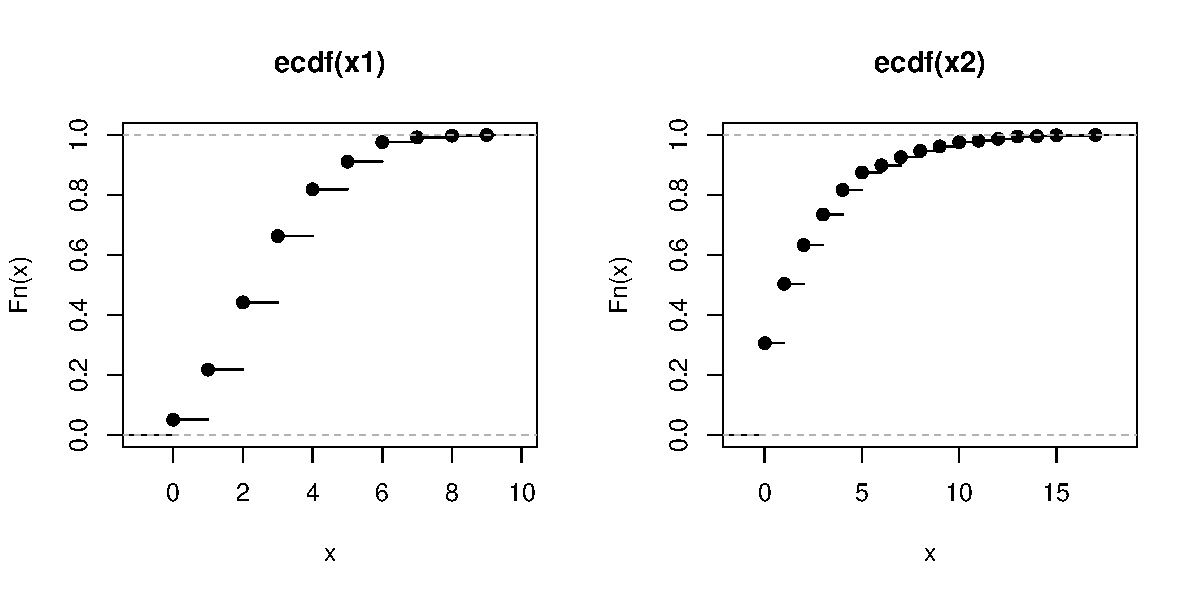
\includegraphics[keepaspectratio]{chapters/ch08_files/figure-pdf/unnamed-chunk-19-1.pdf}}
\end{center}

Recall that every result in R is an object. The output of the function
\texttt{ecdf()} is actually another function that calculates the
estimated CDF for a new value. This can be very handy if you want to
interpolate the ECDF to make a smoother curve.

\begin{Shaded}
\begin{Highlighting}[]
\FunctionTok{class}\NormalTok{(}\FunctionTok{ecdf}\NormalTok{(}\FunctionTok{rnorm}\NormalTok{(}\DecValTok{100}\NormalTok{)))}
\end{Highlighting}
\end{Shaded}

\begin{verbatim}
[1] "ecdf"     "stepfun"  "function"
\end{verbatim}

Here is how to use it. The example below can be useful if you need to
calculate the ECDF for values that are not in the original dataset, but
within its domain. In the example below, the ECDF is estimated for x =
30, which is not in the original data \texttt{x}. Notice what happens
for values in \texttt{x1} that are greater than \texttt{max(x)} and less
than \texttt{min(x)}.

\begin{Shaded}
\begin{Highlighting}[]
\FunctionTok{set.seed}\NormalTok{(}\DecValTok{123}\NormalTok{)}
\NormalTok{x }\OtherTok{\textless{}{-}} \FunctionTok{rnorm}\NormalTok{(}\FloatTok{1e2}\NormalTok{, }\DecValTok{20}\NormalTok{, }\DecValTok{5}\NormalTok{)}
\NormalTok{e1 }\OtherTok{\textless{}{-}} \FunctionTok{ecdf}\NormalTok{(x) }\CommentTok{\# define function for CDF(x)}
\NormalTok{x1 }\OtherTok{\textless{}{-}} \DecValTok{0}\SpecialCharTok{:}\DecValTok{100}  \CommentTok{\# define new x values at which to calculate CDF}
\NormalTok{y1 }\OtherTok{\textless{}{-}} \FunctionTok{e1}\NormalTok{(x1) }\CommentTok{\# calculate CDF at each new x}
\FunctionTok{par}\NormalTok{(}\AttributeTok{mfrow=}\FunctionTok{c}\NormalTok{(}\DecValTok{1}\NormalTok{,}\DecValTok{1}\NormalTok{))}
\FunctionTok{plot}\NormalTok{(x1, y1, }\AttributeTok{type=}\StringTok{"s"}\NormalTok{, }\AttributeTok{lwd=}\DecValTok{2}\NormalTok{, }\AttributeTok{col=}\StringTok{"blue2"}\NormalTok{)}
\end{Highlighting}
\end{Shaded}

\begin{center}
\pandocbounded{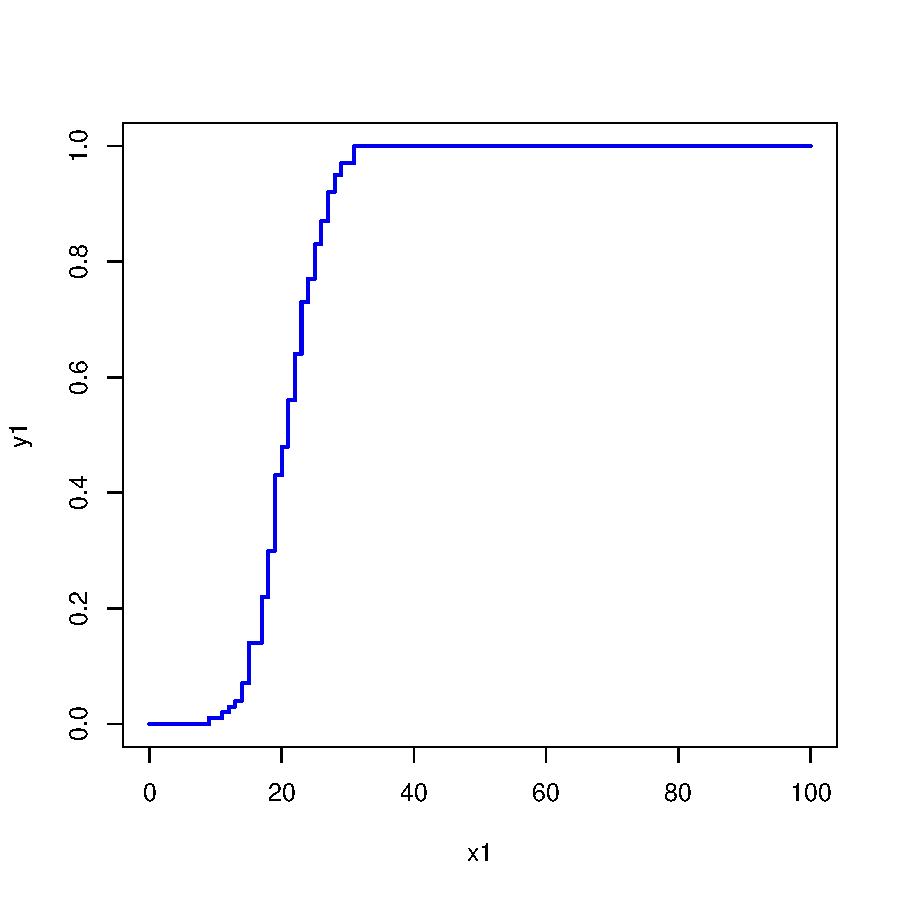
\includegraphics[keepaspectratio]{chapters/ch08_files/figure-pdf/unnamed-chunk-21-1.pdf}}
\end{center}

Obviously, the more data points you have, the better and smoother the
estimate of the ECDF will be. Consider the simulated example below that
estimates the ECDF using different numbers of points.

\begin{Shaded}
\begin{Highlighting}[]
\FunctionTok{set.seed}\NormalTok{(}\DecValTok{123}\NormalTok{)}
\NormalTok{n }\OtherTok{\textless{}{-}} \FloatTok{1e4}
\NormalTok{mu }\OtherTok{\textless{}{-}} \DecValTok{20}
\NormalTok{sig }\OtherTok{\textless{}{-}} \DecValTok{5}
\NormalTok{x4 }\OtherTok{\textless{}{-}} \FunctionTok{rnorm}\NormalTok{(n, mu, sig)}
\NormalTok{x1 }\OtherTok{\textless{}{-}}\NormalTok{ x4[}\FunctionTok{sample}\NormalTok{(}\DecValTok{1}\SpecialCharTok{:}\NormalTok{n, }\DecValTok{10}\NormalTok{, }\AttributeTok{replace=}\ConstantTok{TRUE}\NormalTok{)]}
\NormalTok{x2 }\OtherTok{\textless{}{-}}\NormalTok{ x4[}\FunctionTok{sample}\NormalTok{(}\DecValTok{1}\SpecialCharTok{:}\NormalTok{n, }\DecValTok{100}\NormalTok{, }\AttributeTok{replace=}\ConstantTok{TRUE}\NormalTok{)]}
\NormalTok{x3 }\OtherTok{\textless{}{-}}\NormalTok{ x4[}\FunctionTok{sample}\NormalTok{(}\DecValTok{1}\SpecialCharTok{:}\NormalTok{n, }\DecValTok{1000}\NormalTok{, }\AttributeTok{replace=}\ConstantTok{TRUE}\NormalTok{)]}

\NormalTok{xseq }\OtherTok{\textless{}{-}} \FunctionTok{seq}\NormalTok{(}\DecValTok{0}\NormalTok{, }\DecValTok{40}\NormalTok{, }\AttributeTok{length=}\DecValTok{100}\NormalTok{)}
\NormalTok{y1 }\OtherTok{\textless{}{-}} \FunctionTok{ecdf}\NormalTok{(x1)(xseq)}
\NormalTok{y2 }\OtherTok{\textless{}{-}} \FunctionTok{ecdf}\NormalTok{(x2)(xseq)}
\NormalTok{y3 }\OtherTok{\textless{}{-}} \FunctionTok{ecdf}\NormalTok{(x3)(xseq)}
\NormalTok{yt }\OtherTok{\textless{}{-}} \FunctionTok{pnorm}\NormalTok{(xseq, mu, sig)}

\FunctionTok{plot}\NormalTok{(xseq, yt, }\AttributeTok{type=}\StringTok{"l"}\NormalTok{, }\AttributeTok{lwd=}\DecValTok{6}\NormalTok{, }\AttributeTok{xlab=}\StringTok{"x"}\NormalTok{,}
     \AttributeTok{ylab=}\StringTok{"(E)CDF = F(x)"}\NormalTok{)}
\FunctionTok{points}\NormalTok{(xseq, y1, }\AttributeTok{type=}\StringTok{"l"}\NormalTok{, }\AttributeTok{lwd=}\DecValTok{2}\NormalTok{, }\AttributeTok{col=}\StringTok{"red"}\NormalTok{)}
\FunctionTok{points}\NormalTok{(xseq, y2, }\AttributeTok{type=}\StringTok{"l"}\NormalTok{, }\AttributeTok{lwd=}\DecValTok{2}\NormalTok{, }\AttributeTok{col=}\StringTok{"blue2"}\NormalTok{)}
\FunctionTok{points}\NormalTok{(xseq, y3, }\AttributeTok{type=}\StringTok{"l"}\NormalTok{, }\AttributeTok{lwd=}\DecValTok{2}\NormalTok{, }\AttributeTok{col=}\StringTok{"green"}\NormalTok{)}
\FunctionTok{legend}\NormalTok{(}\StringTok{"topleft"}\NormalTok{, }
    \AttributeTok{legend=}\FunctionTok{c}\NormalTok{(}\FunctionTok{expression}\NormalTok{(n}\SpecialCharTok{==}\DecValTok{10}\NormalTok{), }\FunctionTok{expression}\NormalTok{(n}\SpecialCharTok{==}\DecValTok{100}\NormalTok{), }
             \FunctionTok{expression}\NormalTok{(n}\SpecialCharTok{==}\DecValTok{1000}\NormalTok{), }\StringTok{"True CDF"}\NormalTok{),}
    \AttributeTok{lwd=}\FunctionTok{c}\NormalTok{(}\DecValTok{2}\NormalTok{,}\DecValTok{2}\NormalTok{,}\DecValTok{2}\NormalTok{,}\DecValTok{6}\NormalTok{),}
    \AttributeTok{col=}\FunctionTok{c}\NormalTok{(}\StringTok{"red"}\NormalTok{, }\StringTok{"blue2"}\NormalTok{, }\StringTok{"green"}\NormalTok{, }\StringTok{"black"}\NormalTok{),}
    \AttributeTok{bty=}\StringTok{"n"}\NormalTok{, }\AttributeTok{cex=}\FloatTok{1.2}\NormalTok{)}
\end{Highlighting}
\end{Shaded}

\begin{center}
\pandocbounded{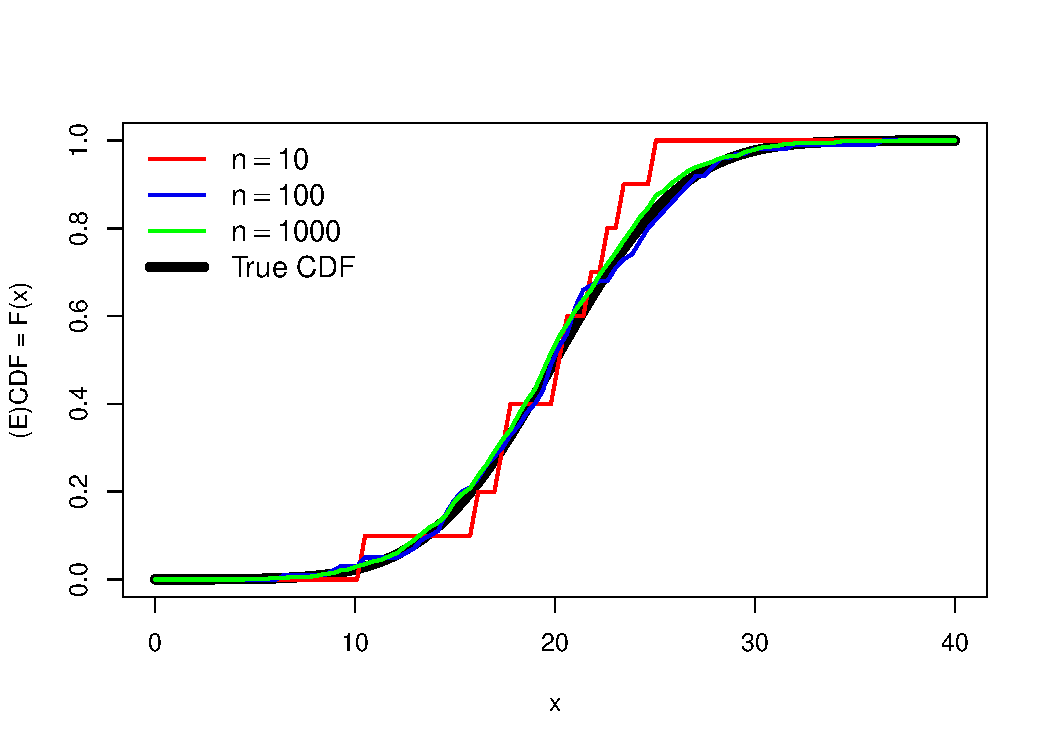
\includegraphics[keepaspectratio]{chapters/ch08_files/figure-pdf/unnamed-chunk-22-1.pdf}}
\end{center}

The estimate with 10 points (red) is a very rough fit, but serviceable.
The estimates using 100 or 1000 points are much closer to the truth
(black line).

\subsection{Kernel density plots}\label{sec-plot1-sing-kern}

Kernel density plots are a way to empirically estimate and visualize the
\textbf{probability distribution function (PDF)} of a distribution
(Section~\ref{sec-dist-cont}). A plot of the estimated PDF is
essentially a histogram where the bin width approaches 0. The PDF tells
us two things. Practically speaking, the PDF of a distribution at a
given value is related to how likely that value is to occur relative to
other values. However, that is NOT the same as the probability of that
value occurring.

What the PDF really expresses is the \emph{rate of change in cumulative
density at a value}.

\begin{itemize}
\tightlist
\item
  The \textbf{cumulative density} of a distribution at some value
  \emph{x} is the probability of a value \(\le\) \emph{x}.
\item
  The \textbf{cumulative density function (CDF)} gives the cumulative
  density at \emph{x}.
\end{itemize}

The PDF is defined as is the \emph{slope or first derivative of the
CDF}. Conversely, the CDF is the integral of the PDF. The PDF is the
rate at which the probability of observing a value \(\le{x}\) increases
at each \(x\). Again, this is related to but not the same as the
probability of that value occurring.

\pandocbounded{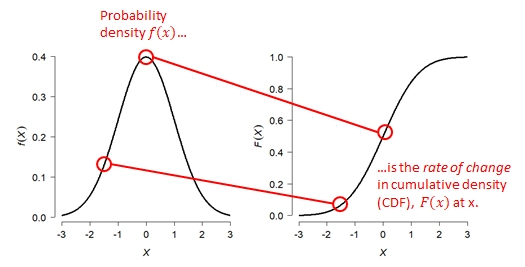
\includegraphics[keepaspectratio,alt={Relationship between the probability density function (PDF) (left) and cumulative distribution function (CDF) (right) of a distribution. The PDF at some x value is the slope of the CDF at that x value. The CDF at some x value is the integral of the PDF up to that x value.}]{chapters/../images/08-02.jpg}}\{fig-alt:``Relationship
between the probability density function (PDF) and cumulative
distribution function (CDF) of a normal distribution. The left panel
shows the PDF, f(x), as a bell-shaped curve. The right panel shows the
corresponding CDF, F(x), as an S-shaped curve increasing from 0 to 1.
Red annotations connect corresponding values of x on the two graphs,
illustrating that the probability density f(x) at a given value equals
the rate of change (slope) of the cumulative distribution function F(x)
at that same value. Larger PDF values correspond to steeper slopes of
the CDF, while smaller PDF values correspond to flatter portions of the
CDF.''\}

The kernel density plot estimated by R is to the PDF what the empirical
cumulative distribution function (ECDF; see
Section~\ref{sec-plot1-sing-cdf}) is to the CDF. Just like an ECDF plot
presents an estimate of the true CDF, the kernel density plot presents
an estimate of the true PDF. This means that presenting a kernel density
plot or an ECDF plot is largely a matter of preference because they
convey the same information in different ways.

Note that a kernel density plot makes more sense for a
\href{@sec-dist-cont}{continuous distribution} than for a
\href{@sec-dist-disc}{discrete distribution}. The equivalent plot for a
discrete distribution is the \textbf{probability mass function (PMF)}
plot, which looks like a barplot because the PMF is only non-zero for
integer values.

The example below shows kernel density plots for four distributions:
\(Normal\left(\mu=5,\sigma=2\right)\),
\(Gamma\left(k=3,\theta=2\right)\), \(Uniform\left(min=0,max=1\right)\),
and \(Poisson\left(\lambda=4\right)\). The first 3 are continuous
distributions and the last is a discrete distribution.

\begin{Shaded}
\begin{Highlighting}[]
\FunctionTok{set.seed}\NormalTok{(}\DecValTok{123}\NormalTok{)}
\NormalTok{n }\OtherTok{\textless{}{-}} \FloatTok{1e3}
\FunctionTok{par}\NormalTok{(}\AttributeTok{mfrow=}\FunctionTok{c}\NormalTok{(}\DecValTok{2}\NormalTok{,}\DecValTok{2}\NormalTok{))}
\FunctionTok{plot}\NormalTok{(}\FunctionTok{density}\NormalTok{(}\FunctionTok{rnorm}\NormalTok{(n,}\DecValTok{5}\NormalTok{,}\DecValTok{2}\NormalTok{)), }\AttributeTok{main=}\StringTok{"Normal(5, 2)"}\NormalTok{)}
\FunctionTok{plot}\NormalTok{(}\FunctionTok{density}\NormalTok{(}\FunctionTok{rgamma}\NormalTok{(n, }\DecValTok{3}\NormalTok{, }\DecValTok{2}\NormalTok{)), }\AttributeTok{main=}\StringTok{"Gamma(3, 2)"}\NormalTok{)}
\FunctionTok{plot}\NormalTok{(}\FunctionTok{density}\NormalTok{(}\FunctionTok{runif}\NormalTok{(n)), }\AttributeTok{main=}\StringTok{"Uniform(0, 1)"}\NormalTok{)}
\FunctionTok{plot}\NormalTok{(}\FunctionTok{density}\NormalTok{(}\FunctionTok{rpois}\NormalTok{(n,}\DecValTok{4}\NormalTok{)), }\AttributeTok{main=}\StringTok{"Poisson(4)"}\NormalTok{)}
\end{Highlighting}
\end{Shaded}

\pandocbounded{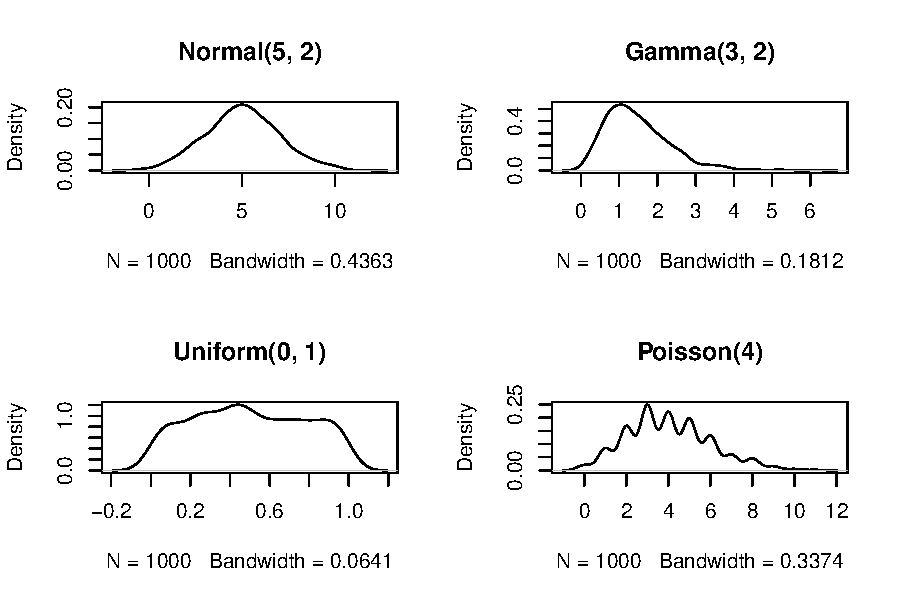
\includegraphics[keepaspectratio]{chapters/ch08_files/figure-pdf/unnamed-chunk-23-1.pdf}}

The estimated density functions aren't too far off from the real
functions. But, notice that the plots for the gamma, uniform, and
Poisson variables extend outside of the domains of the underlying
distributions. For example, the density for the Poisson variable extends
below 0--because the Poisson distribution models counts, it is only
supported for non-negative integers (think about why\ldots you can't
count -3 or 2.5 fish). You can truncate the plot using arguments
\texttt{from} or \texttt{to} for density. This is a good idea if you are
exploring data that you suspect have a natural domain.

For example, lengths and times must be non-negative, so you should
include \texttt{from=0} in the \texttt{density()} command.

\begin{Shaded}
\begin{Highlighting}[]
\FunctionTok{par}\NormalTok{(}\AttributeTok{mfrow=}\FunctionTok{c}\NormalTok{(}\DecValTok{2}\NormalTok{,}\DecValTok{2}\NormalTok{))}
\FunctionTok{plot}\NormalTok{(}\FunctionTok{density}\NormalTok{(}\FunctionTok{rnorm}\NormalTok{(n,}\DecValTok{5}\NormalTok{,}\DecValTok{2}\NormalTok{)), }\AttributeTok{main=}\StringTok{"Normal(5, 2)"}\NormalTok{)}
\FunctionTok{plot}\NormalTok{(}\FunctionTok{density}\NormalTok{(}\FunctionTok{rgamma}\NormalTok{(n, }\DecValTok{3}\NormalTok{, }\DecValTok{2}\NormalTok{), }\AttributeTok{from=}\DecValTok{0}\NormalTok{), }\AttributeTok{main=}\StringTok{"Gamma(3, 2)"}\NormalTok{)}
\FunctionTok{plot}\NormalTok{(}\FunctionTok{density}\NormalTok{(}\FunctionTok{runif}\NormalTok{(n), }\AttributeTok{from=}\DecValTok{0}\NormalTok{, }\AttributeTok{to=}\DecValTok{1}\NormalTok{), }\AttributeTok{main=}\StringTok{"Uniform(0, 1)"}\NormalTok{)}
\FunctionTok{plot}\NormalTok{(}\FunctionTok{density}\NormalTok{(}\FunctionTok{rpois}\NormalTok{(n,}\DecValTok{4}\NormalTok{), }\AttributeTok{from=}\DecValTok{0}\NormalTok{), }\AttributeTok{main=}\StringTok{"Poisson(4)"}\NormalTok{)}
\end{Highlighting}
\end{Shaded}

\pandocbounded{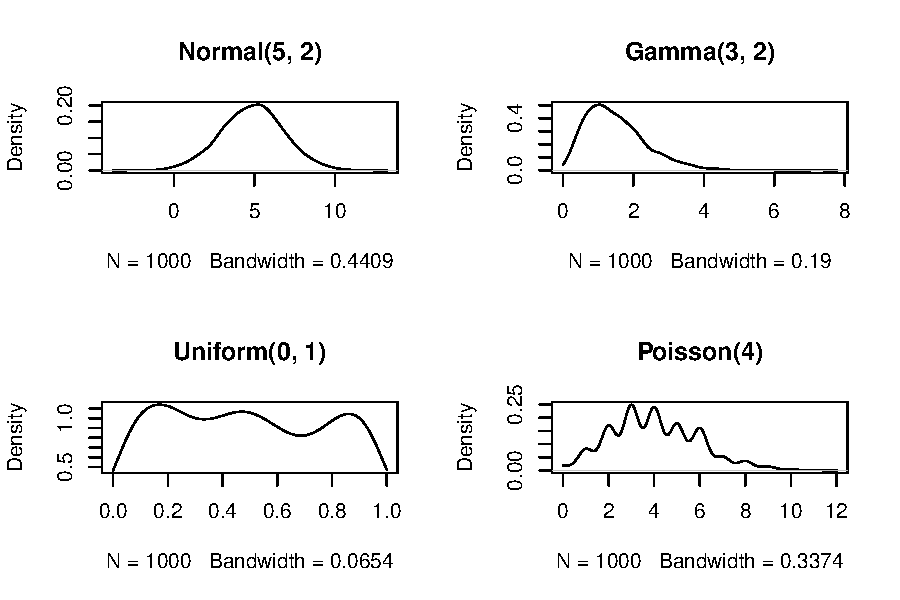
\includegraphics[keepaspectratio]{chapters/ch08_files/figure-pdf/unnamed-chunk-24-1.pdf}}

The estimated density functions are now in their supported intervals,
which is nice. There's one more issue with the estimates for the Poisson
distribution. Notice that the bottom right plot shows non-zero
probability density for non-integer values. This doesn't make sense for
a Poisson distribution, which can only take non-negative integer values.
What's going on here is that the \texttt{density()} function does not
know whether a distribution is supposed to be discrete or continuous. As
far as the function is concerned, the distribution is continuous and
just happens to have no non-integer values.

If you have data that you have good reason to suspect are discrete,
there is a better way than \texttt{density()} to visualize the relative
likelihood of different values: the \textbf{probability mass function
(PMF, not PDF)}. The PMF of a discrete distribution can be calculated
rather than estimated.

In the example below we use the \texttt{table()} function, which tallies
up the number of times each value occurs in a vector. We could convert
the cell counts to PMF estimates by dividing by the number of
observations (e.g., \texttt{plot(table(x1)/n))}.

\begin{Shaded}
\begin{Highlighting}[]
\CommentTok{\# make some data}
\FunctionTok{set.seed}\NormalTok{(}\DecValTok{42}\NormalTok{)}
\NormalTok{n }\OtherTok{\textless{}{-}} \FloatTok{1e3}
\NormalTok{x1 }\OtherTok{\textless{}{-}} \FunctionTok{rpois}\NormalTok{(n, }\DecValTok{4}\NormalTok{)}
\NormalTok{x2 }\OtherTok{\textless{}{-}} \FunctionTok{rbinom}\NormalTok{(n, }\DecValTok{20}\NormalTok{, }\FloatTok{0.4}\NormalTok{)}
\NormalTok{x3 }\OtherTok{\textless{}{-}} \FunctionTok{rgeom}\NormalTok{(n, }\FloatTok{0.3}\NormalTok{)}
\NormalTok{x4 }\OtherTok{\textless{}{-}} \FunctionTok{rnbinom}\NormalTok{(n, }\DecValTok{10}\NormalTok{, }\FloatTok{0.1}\NormalTok{)}

\CommentTok{\# plot cell counts:}
\FunctionTok{par}\NormalTok{(}\AttributeTok{mfrow=}\FunctionTok{c}\NormalTok{(}\DecValTok{2}\NormalTok{,}\DecValTok{2}\NormalTok{))}
\FunctionTok{plot}\NormalTok{(}\FunctionTok{table}\NormalTok{(x1))}
\FunctionTok{plot}\NormalTok{(}\FunctionTok{table}\NormalTok{(x2))}
\FunctionTok{plot}\NormalTok{(}\FunctionTok{table}\NormalTok{(x3))}
\FunctionTok{plot}\NormalTok{(}\FunctionTok{table}\NormalTok{(x4))}
\end{Highlighting}
\end{Shaded}

\pandocbounded{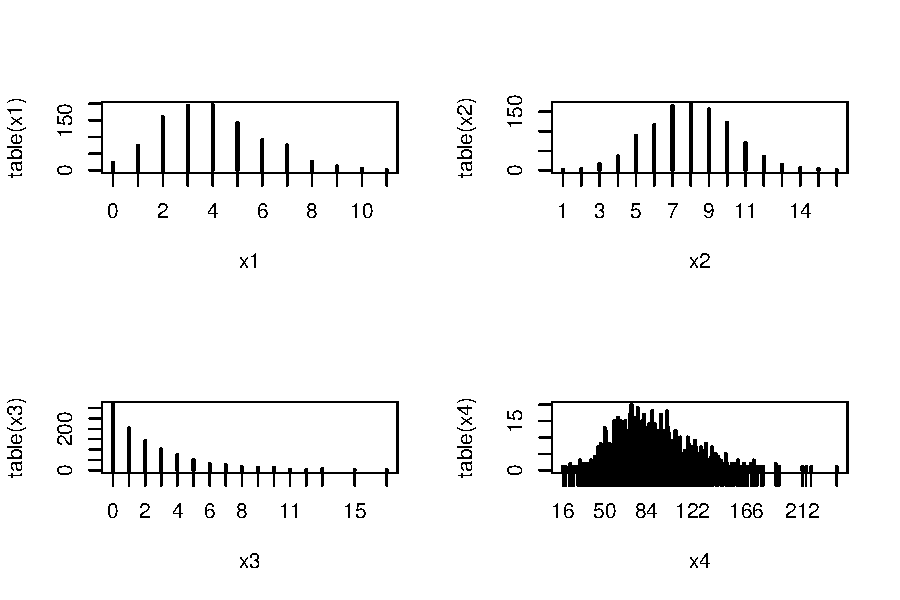
\includegraphics[keepaspectratio]{chapters/ch08_files/figure-pdf/unnamed-chunk-25-1.pdf}}

Dividing the cell counts by the number of total observations (n)
estimates the empirical PMF:

\begin{Shaded}
\begin{Highlighting}[]
\FunctionTok{par}\NormalTok{(}\AttributeTok{mfrow=}\FunctionTok{c}\NormalTok{(}\DecValTok{2}\NormalTok{,}\DecValTok{2}\NormalTok{))}
\FunctionTok{plot}\NormalTok{(}\FunctionTok{table}\NormalTok{(x1)}\SpecialCharTok{/}\NormalTok{n, }\AttributeTok{ylab=}\StringTok{"Empirical PMF"}\NormalTok{)}
\FunctionTok{plot}\NormalTok{(}\FunctionTok{table}\NormalTok{(x2)}\SpecialCharTok{/}\NormalTok{n, }\AttributeTok{ylab=}\StringTok{"Empirical PMF"}\NormalTok{)}
\FunctionTok{plot}\NormalTok{(}\FunctionTok{table}\NormalTok{(x3)}\SpecialCharTok{/}\NormalTok{n, }\AttributeTok{ylab=}\StringTok{"Empirical PMF"}\NormalTok{)}
\FunctionTok{plot}\NormalTok{(}\FunctionTok{table}\NormalTok{(x4)}\SpecialCharTok{/}\NormalTok{n, }\AttributeTok{ylab=}\StringTok{"Empirical PMF"}\NormalTok{)}
\end{Highlighting}
\end{Shaded}

\pandocbounded{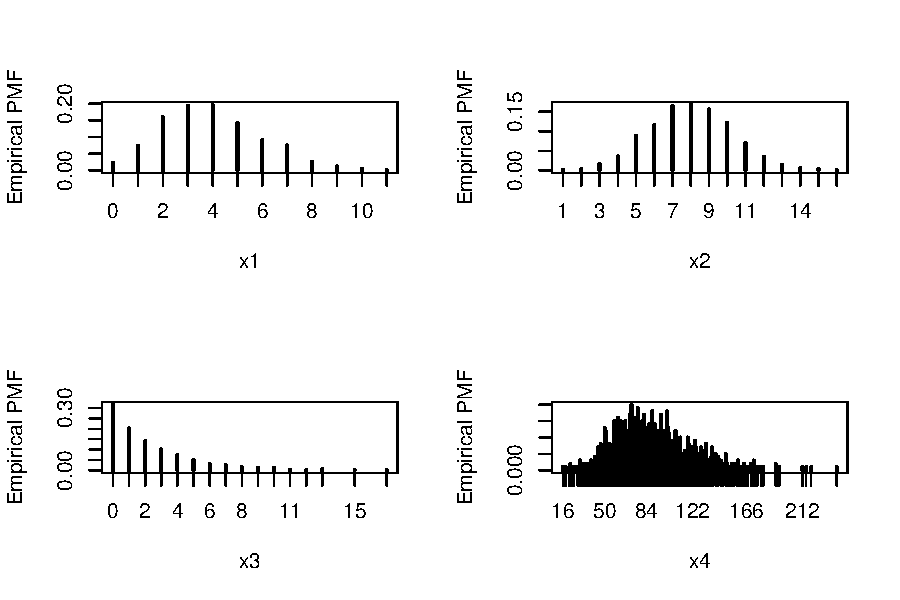
\includegraphics[keepaspectratio]{chapters/ch08_files/figure-pdf/unnamed-chunk-26-1.pdf}}

We can verify that the empirical PMFs that we calculated match the
actual PMFs:

\begin{Shaded}
\begin{Highlighting}[]
\CommentTok{\# compare to true PMF:}
\NormalTok{v1 }\OtherTok{\textless{}{-}} \DecValTok{0}\SpecialCharTok{:}\FunctionTok{max}\NormalTok{(x1)}
\NormalTok{v2 }\OtherTok{\textless{}{-}} \DecValTok{0}\SpecialCharTok{:}\FunctionTok{max}\NormalTok{(x2)}
\NormalTok{v3 }\OtherTok{\textless{}{-}} \DecValTok{0}\SpecialCharTok{:}\FunctionTok{max}\NormalTok{(x3)}
\NormalTok{v4 }\OtherTok{\textless{}{-}} \DecValTok{0}\SpecialCharTok{:}\FunctionTok{max}\NormalTok{(x4)}
\NormalTok{y1 }\OtherTok{\textless{}{-}} \FunctionTok{dpois}\NormalTok{(v1, }\DecValTok{4}\NormalTok{)}
\NormalTok{y2 }\OtherTok{\textless{}{-}} \FunctionTok{dbinom}\NormalTok{(v2, }\DecValTok{20}\NormalTok{, }\FloatTok{0.4}\NormalTok{)}
\NormalTok{y3 }\OtherTok{\textless{}{-}} \FunctionTok{dgeom}\NormalTok{(v3, }\FloatTok{0.3}\NormalTok{)}
\NormalTok{y4 }\OtherTok{\textless{}{-}} \FunctionTok{dnbinom}\NormalTok{(v4, }\DecValTok{10}\NormalTok{, }\FloatTok{0.1}\NormalTok{)}

\FunctionTok{par}\NormalTok{(}\AttributeTok{mfrow=}\FunctionTok{c}\NormalTok{(}\DecValTok{2}\NormalTok{,}\DecValTok{2}\NormalTok{))}
\FunctionTok{plot}\NormalTok{(}\FunctionTok{table}\NormalTok{(x1)}\SpecialCharTok{/}\NormalTok{n)}
\FunctionTok{points}\NormalTok{(v1, y1, }\AttributeTok{type=}\StringTok{"l"}\NormalTok{, }\AttributeTok{col=}\StringTok{"red"}\NormalTok{, }\AttributeTok{lwd=}\DecValTok{2}\NormalTok{)}
\FunctionTok{plot}\NormalTok{(}\FunctionTok{table}\NormalTok{(x2)}\SpecialCharTok{/}\NormalTok{n)}
\FunctionTok{points}\NormalTok{(v2, y2, }\AttributeTok{type=}\StringTok{"l"}\NormalTok{, }\AttributeTok{col=}\StringTok{"red"}\NormalTok{, }\AttributeTok{lwd=}\DecValTok{2}\NormalTok{)}
\FunctionTok{plot}\NormalTok{(}\FunctionTok{table}\NormalTok{(x3)}\SpecialCharTok{/}\NormalTok{n)}
\FunctionTok{points}\NormalTok{(v3, y3, }\AttributeTok{type=}\StringTok{"l"}\NormalTok{, }\AttributeTok{col=}\StringTok{"red"}\NormalTok{, }\AttributeTok{lwd=}\DecValTok{2}\NormalTok{)}
\FunctionTok{plot}\NormalTok{(}\FunctionTok{table}\NormalTok{(x4)}\SpecialCharTok{/}\NormalTok{n)}
\FunctionTok{points}\NormalTok{(v4, y4, }\AttributeTok{type=}\StringTok{"l"}\NormalTok{, }\AttributeTok{col=}\StringTok{"red"}\NormalTok{, }\AttributeTok{lwd=}\DecValTok{2}\NormalTok{)}
\end{Highlighting}
\end{Shaded}

\begin{center}
\pandocbounded{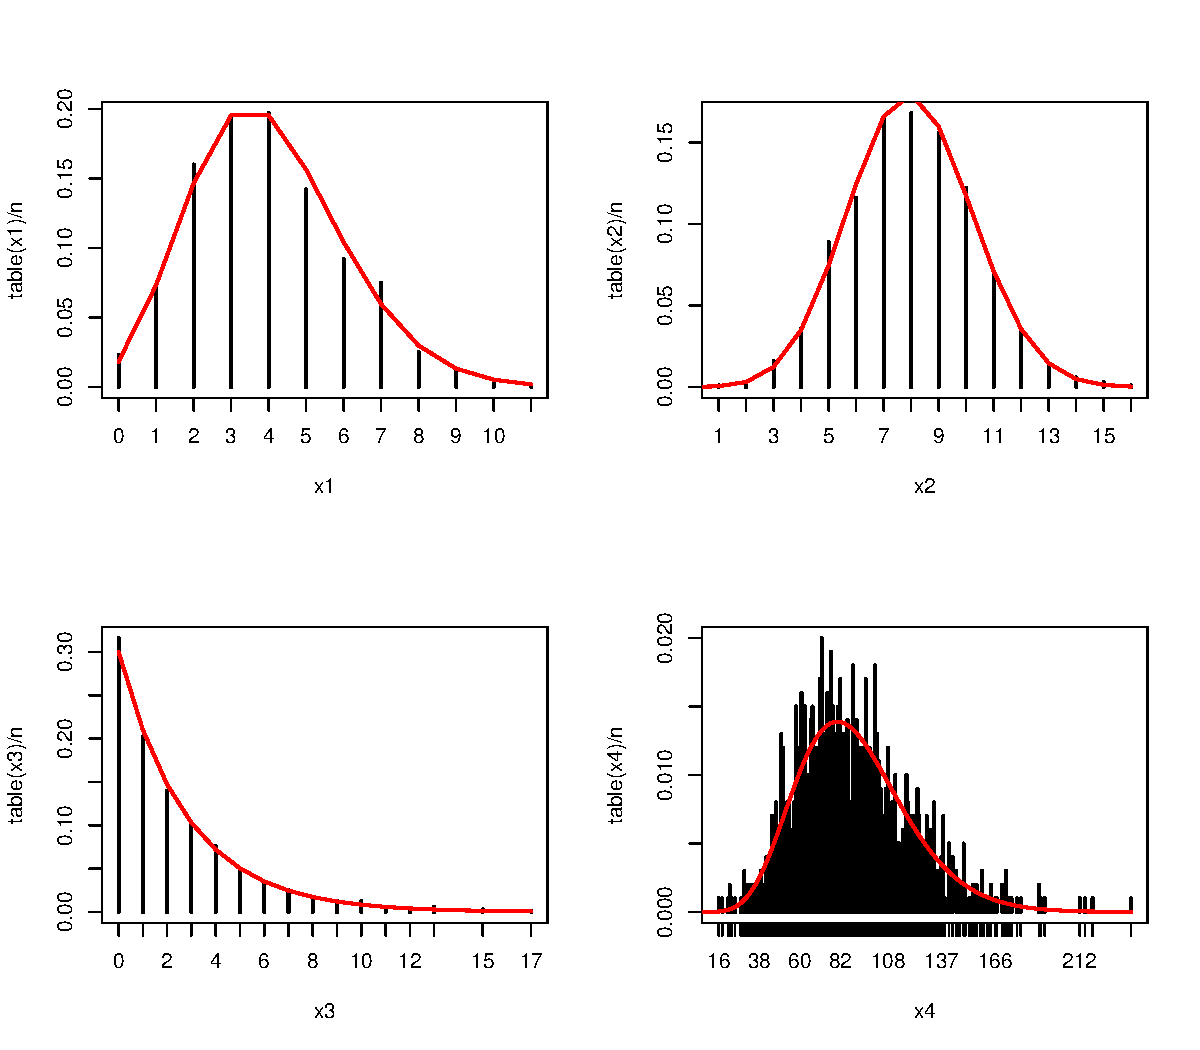
\includegraphics[keepaspectratio]{chapters/ch08_files/figure-pdf/unnamed-chunk-27-1.pdf}}
\end{center}

\section{Visualizing 2 variables}\label{sec-plot1-two}

So far in this course we have explored ways to
\hyperref[sec-dist-single]{explore distributions of single variables}:
histograms, ECDF plots, probability density plots, and so on. In this
section we will explore ways to explore relationships \emph{between}
variables. This is a vital preliminary step in studying how two or more
variables might be correlated with each other, or how one might cause
the other. The focus on this page is on exploratory, correlative
methods. Actual inference about relationships between two variables is
better handled by \href{@sec-14-lin}{linear models (LM)},
\href{@sec-16}{generalized linear models (GLM)}, or \href{@sec-20}{other
kinds of models}.

\subsection{Scatterplots for 2 continuous
variables}\label{sec-plot1-two-scatter}

The \textbf{scatterplot} is one of the most important tools in the
biologist's data toolbox. It is probably the simplest type of figure in
routine use: simply plot the values in one variable on one axis, and the
values of another variable on another (perpendicular) axis. The role of
the scatterplot in exploratory data analysis is to help visualize the
form of the relationship between two variables (Bolker 2008). The figure
below shows just 6 of the possible curve types that you might discover.

\begin{center}
\pandocbounded{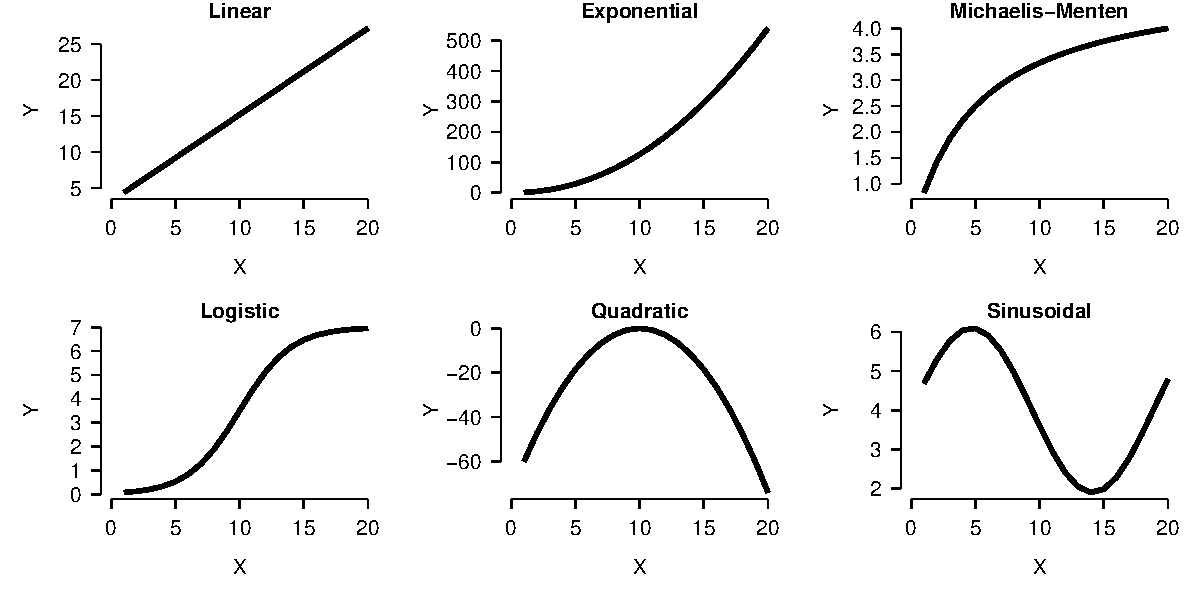
\includegraphics[keepaspectratio]{chapters/ch08_files/figure-pdf/unnamed-chunk-28-1.pdf}}
\end{center}

\subsubsection{R plotting basics}\label{r-plotting-basics}

We have already made some scatterplots, but it's worth taking a closer
look at the R methods for scatterplots. The basic function for
scatterplots is \texttt{plot()}. The first argument is taken to be the x
coordinates, and the second argument to be the y coordinates. You can
also use the formula interface \texttt{plot(y\ \textasciitilde{}\ x)},
but the coordinates method \texttt{plot(x,\ y)} usually makes for
cleaner code.

Calling \texttt{plot()} does two things: first, it \emph{creates a new
plot}; second, it \emph{plots the data} on the new plot area. Other
components can be added to the plot with subsequent commands:

\begin{itemize}
\tightlist
\item
  \texttt{points()} for points
\item
  \texttt{text()} for text
\item
  \texttt{lines()} for lines
\item
  \texttt{polygon()} for polygons
\item
  \texttt{segments()} for line segments
\end{itemize}

and so on. These functions will \textbf{\emph{add}} to an existing plot,
but will not create a new plot area. So, call \texttt{plot()} first,
then \texttt{points()} or one of the others if needed. Calling
\texttt{points()} or one of the ``adding'' functions if there is not
already an active plot area will return an error.

Here is a basic scatterplot:

\begin{Shaded}
\begin{Highlighting}[]
\FunctionTok{plot}\NormalTok{(iris}\SpecialCharTok{$}\NormalTok{Petal.Width,iris}\SpecialCharTok{$}\NormalTok{Petal.Length)}
\end{Highlighting}
\end{Shaded}

\pandocbounded{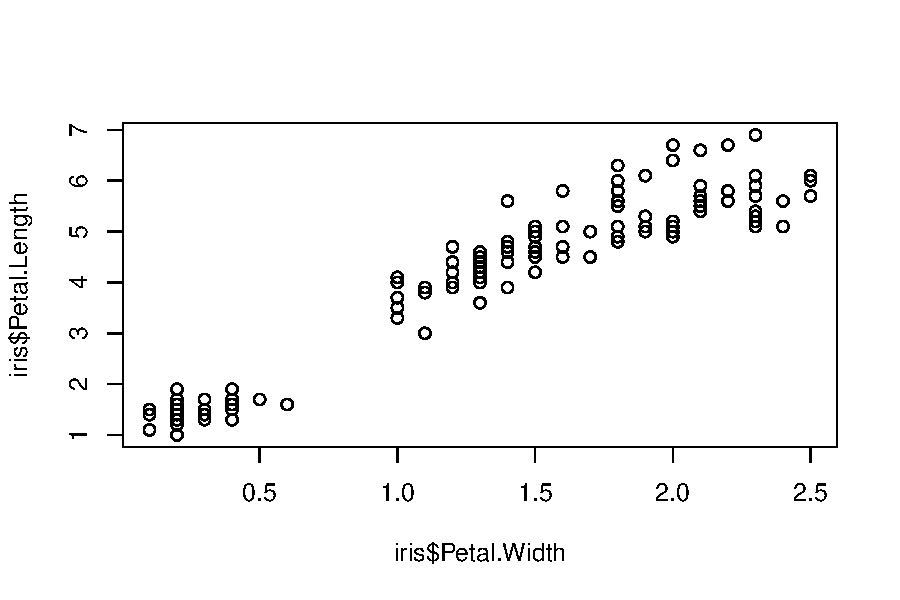
\includegraphics[keepaspectratio]{chapters/ch08_files/figure-pdf/unnamed-chunk-29-1.pdf}}

The default scatterplot is rather unattractive, but works just fine for
exploring data. Fortunately, almost every aspect of a plot can be
customized using different plot arguments and graphical parameters. Here
are some commonly used plot options:

\begin{Shaded}
\begin{Highlighting}[]
\FunctionTok{plot}\NormalTok{(iris}\SpecialCharTok{$}\NormalTok{Petal.Width,iris}\SpecialCharTok{$}\NormalTok{Petal.Length,}
    \AttributeTok{xlab=}\StringTok{"Petal width (cm)"}\NormalTok{,             }\CommentTok{\# x label}
    \AttributeTok{ylab=}\StringTok{"Petal Length (cm)"}\NormalTok{,            }\CommentTok{\# y label}
    \AttributeTok{xlim=}\FunctionTok{c}\NormalTok{(}\DecValTok{0}\NormalTok{,}\DecValTok{3}\NormalTok{),                         }\CommentTok{\# x axis limits}
    \AttributeTok{ylim=}\FunctionTok{c}\NormalTok{(}\DecValTok{0}\NormalTok{,}\DecValTok{8}\NormalTok{),                         }\CommentTok{\# y axis limits}
    \AttributeTok{main=}\StringTok{"Petal length vs. petal width"}  \CommentTok{\# plot title}
\NormalTok{)}\CommentTok{\#plot}
\end{Highlighting}
\end{Shaded}

\pandocbounded{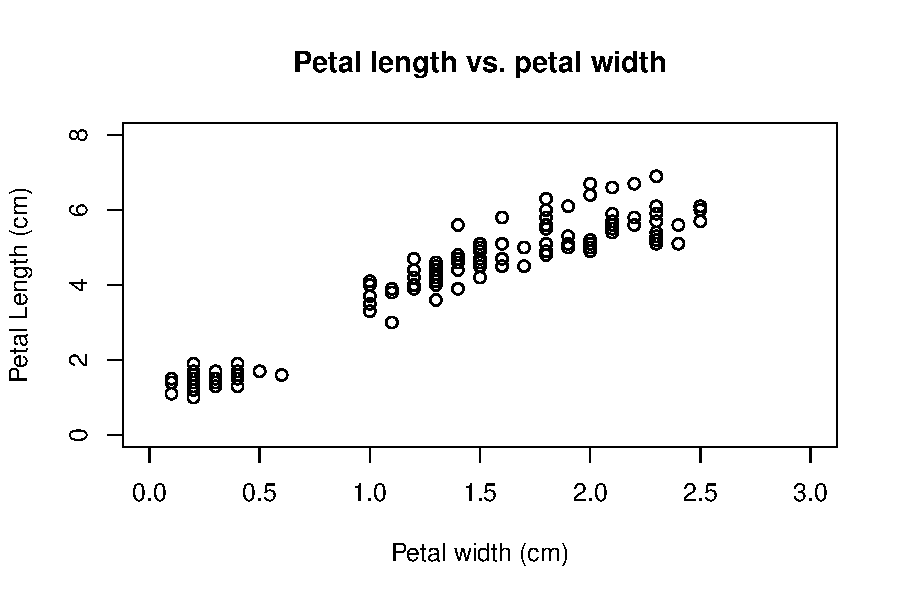
\includegraphics[keepaspectratio]{chapters/ch08_files/figure-pdf/unnamed-chunk-30-1.pdf}}

Sometimes it helps to change the color or style of points to show
categories in the data. This can be done using some arguments to
\texttt{plot()}:

\begin{itemize}
\tightlist
\item
  \texttt{pch} changes the symbol used for points. Think
  ``\textbf{p}oint \textbf{ch}aracter''. See \texttt{?points} for a list
  of available symbols.
\item
  \texttt{cex} changes the size of symbols. Think ``\textbf{c}haracter
  \textbf{ex}pansion''. The default \texttt{cex} is 1; other values
  scale the points relative to this. E.g., \texttt{cex=2} makes points
  twice as large.
\item
  \texttt{col} changes the color. Think ``\textbf{col}or''. R can
  produce many colors; run the command \texttt{colors()} to see a named
  list\footnote{You can also specify colors by their RGB or hex codes.
    Just google ``R color chart'' to get some examples. The
    \href{https://colorbrewer2.org/}{ColorBrewer} website (accessed
    2026-08-05) and R package can help picking appropriate color
    schemes.}.
\end{itemize}

Each these arguments can take vector of values, so you can assign colors
or shape to each point. The values will be used in the same order as the
observations used to draw the points (e.g., rows of a data frame). I
find it convenient to put colors, shapes, and other point-specific
graphical parameters into the dataframe that contains the coordinates.
That way, if I ever subset the data frame, or sort the data frame, the
symbology information stays with each point.

The examples below illustrate several ways of assigning symbology to
observations within a data frame. In the first, \texttt{ifelse()} is
used to make vectors of colors (\texttt{use.col}) defined by the
variable \texttt{species}. Notice that a legend is provided to tell the
reader which symbols mean what. This method works fine if you only have
a few groups to define symbols for.

\begin{Shaded}
\begin{Highlighting}[]
\CommentTok{\# method 1: ifelse()}
\NormalTok{iris}\SpecialCharTok{$}\NormalTok{color }\OtherTok{\textless{}{-}} \FunctionTok{ifelse}\NormalTok{(iris}\SpecialCharTok{$}\NormalTok{Species }\SpecialCharTok{==} \StringTok{"setosa"}\NormalTok{, }\StringTok{"black"}\NormalTok{, }
    \FunctionTok{ifelse}\NormalTok{(iris}\SpecialCharTok{$}\NormalTok{Species }\SpecialCharTok{==} \StringTok{"versicolor"}\NormalTok{, }\StringTok{"red"}\NormalTok{, }\StringTok{"blue"}\NormalTok{))}

\FunctionTok{plot}\NormalTok{(iris}\SpecialCharTok{$}\NormalTok{Petal.Width,iris}\SpecialCharTok{$}\NormalTok{Petal.Length,}
    \AttributeTok{col=}\NormalTok{iris}\SpecialCharTok{$}\NormalTok{color, }\CommentTok{\# color by species}
    \AttributeTok{pch=}\DecValTok{16}       \CommentTok{\# solid dots   }
\NormalTok{)}
\FunctionTok{legend}\NormalTok{(}\StringTok{"bottomright"}\NormalTok{, }
    \AttributeTok{legend=}\FunctionTok{c}\NormalTok{(}\StringTok{"Setosa"}\NormalTok{, }\StringTok{"Versicolor"}\NormalTok{, }\StringTok{"Virginica"}\NormalTok{),}
    \AttributeTok{pch=}\DecValTok{16}\NormalTok{, }\AttributeTok{col=}\FunctionTok{c}\NormalTok{(}\StringTok{"black"}\NormalTok{, }\StringTok{"red"}\NormalTok{, }\StringTok{"blue"}\NormalTok{))}
\end{Highlighting}
\end{Shaded}

\pandocbounded{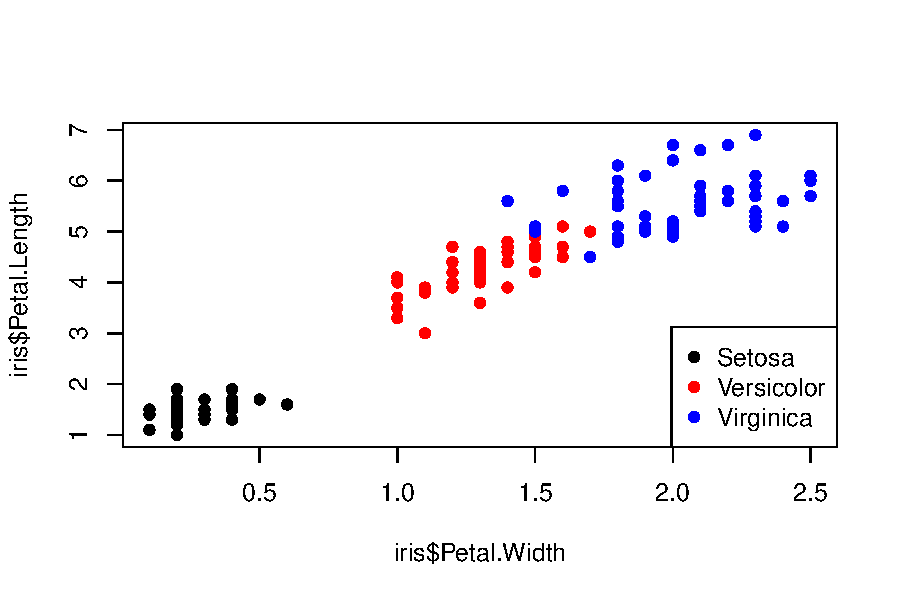
\includegraphics[keepaspectratio]{chapters/ch08_files/figure-pdf/unnamed-chunk-31-1.pdf}}

A better way is to first set up a vector of colors, then name the
elements of the vector, and finally use those names to assign colors to
rows of the data frame. \textbf{\emph{This is the method I use in my
code, and recommend you do too.}} When getting a vector of colors, I
often use \href{https://colorbrewer2.org/}{colorbrewer2} (date accessed
2026-08-05). Notice in the \texttt{legend()} code below that we don't
have to retype the species names or colors because they are already in
the object \texttt{spps} and \texttt{cols}.

\begin{Shaded}
\begin{Highlighting}[]
\CommentTok{\# method 2: match()}
\DocumentationTok{\#\#\#\#  recommended method \#\#\#\#}

\DocumentationTok{\#\# get the species names}
\NormalTok{spps }\OtherTok{\textless{}{-}} \FunctionTok{sort}\NormalTok{(}\FunctionTok{unique}\NormalTok{(iris}\SpecialCharTok{$}\NormalTok{Species))}

\DocumentationTok{\#\# vector of colors}
\DocumentationTok{\#\# can also use rainbow() or colorbrewer2.}
\NormalTok{cols }\OtherTok{\textless{}{-}} \FunctionTok{c}\NormalTok{(}\StringTok{"blue"}\NormalTok{, }\StringTok{"yellow"}\NormalTok{, }\StringTok{"purple"}\NormalTok{)}

\DocumentationTok{\#\# assign names to colors}
\FunctionTok{names}\NormalTok{(cols) }\OtherTok{\textless{}{-}}\NormalTok{ spps}

\DocumentationTok{\#\# assign to data frame}
\NormalTok{iris}\SpecialCharTok{$}\NormalTok{color }\OtherTok{\textless{}{-}}\NormalTok{ cols[iris}\SpecialCharTok{$}\NormalTok{Species]}

\DocumentationTok{\#\# use the new colors in a plot:}
\FunctionTok{plot}\NormalTok{(iris}\SpecialCharTok{$}\NormalTok{Petal.Width,iris}\SpecialCharTok{$}\NormalTok{Petal.Length,}
    \AttributeTok{col=}\NormalTok{iris}\SpecialCharTok{$}\NormalTok{color, }\CommentTok{\# color by species}
    \AttributeTok{pch=}\DecValTok{16}      \CommentTok{\# solid dots    }
\NormalTok{)}
\FunctionTok{legend}\NormalTok{(}\StringTok{"bottomright"}\NormalTok{, }\AttributeTok{legend=}\NormalTok{spps, }\AttributeTok{pch=}\DecValTok{16}\NormalTok{, }\AttributeTok{col=}\NormalTok{cols)}
\end{Highlighting}
\end{Shaded}

\pandocbounded{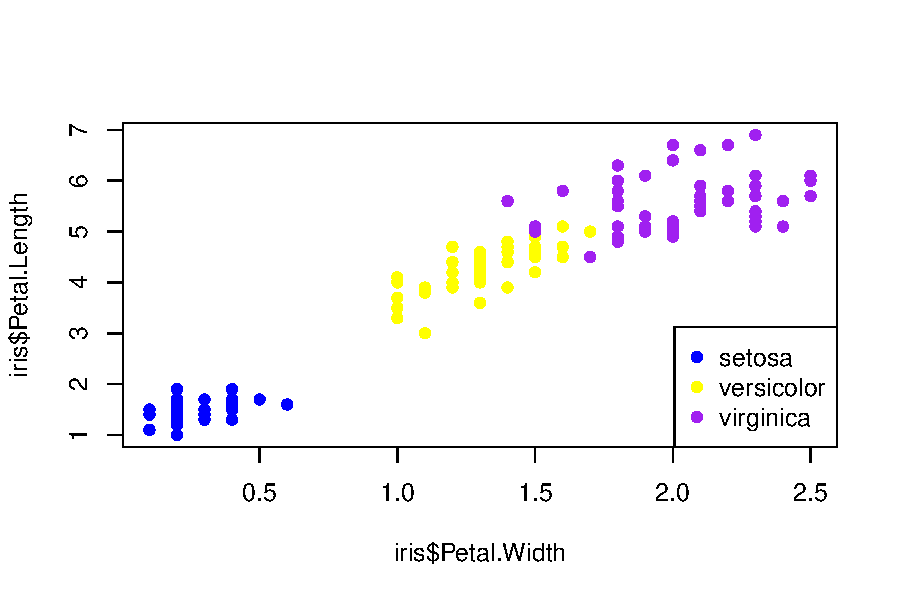
\includegraphics[keepaspectratio]{chapters/ch08_files/figure-pdf/unnamed-chunk-32-1.pdf}}

Below is an example of using shapes (\texttt{use.pch}) to define groups.
See the help page for \texttt{points()} (\texttt{?points}) to see the
available plot symbols. In my plots I usually use both shape and color
to define groups.

\begin{Shaded}
\begin{Highlighting}[]
\CommentTok{\# method 3: names()}
\NormalTok{spps }\OtherTok{\textless{}{-}} \FunctionTok{sort}\NormalTok{(}\FunctionTok{unique}\NormalTok{(iris}\SpecialCharTok{$}\NormalTok{Species))}
\NormalTok{shps }\OtherTok{\textless{}{-}} \FunctionTok{c}\NormalTok{(}\DecValTok{15}\NormalTok{, }\DecValTok{16}\NormalTok{, }\DecValTok{17}\NormalTok{)}
\FunctionTok{names}\NormalTok{(shps) }\OtherTok{\textless{}{-}}\NormalTok{ spps}
\NormalTok{iris}\SpecialCharTok{$}\NormalTok{pch }\OtherTok{\textless{}{-}}\NormalTok{ shps[iris}\SpecialCharTok{$}\NormalTok{Species]}

\FunctionTok{plot}\NormalTok{(iris}\SpecialCharTok{$}\NormalTok{Petal.Width,iris}\SpecialCharTok{$}\NormalTok{Petal.Length,}
     \AttributeTok{pch=}\NormalTok{iris}\SpecialCharTok{$}\NormalTok{pch, }\AttributeTok{col=}\NormalTok{iris}\SpecialCharTok{$}\NormalTok{color)}
\FunctionTok{legend}\NormalTok{(}\StringTok{"bottomright"}\NormalTok{, }\AttributeTok{legend=}\NormalTok{spps, }\AttributeTok{pch=}\NormalTok{shps, }\AttributeTok{col=}\NormalTok{cols)}
\end{Highlighting}
\end{Shaded}

\pandocbounded{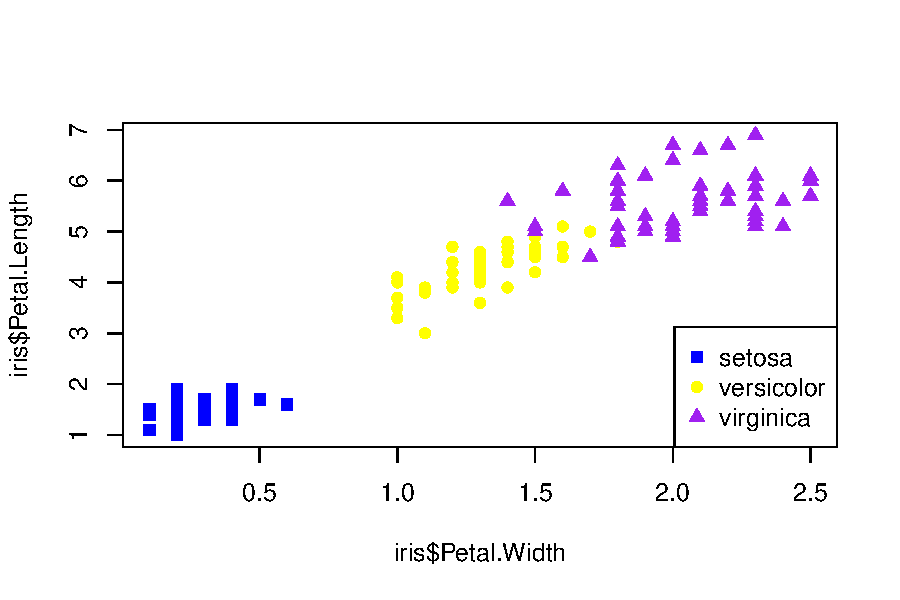
\includegraphics[keepaspectratio]{chapters/ch08_files/figure-pdf/unnamed-chunk-33-1.pdf}}

You can think of the plot generated by \texttt{plot()} like a canvas.
Once the canvas is in place, things can be ``painted'' on, but like
paint cannot be removed. If you want to remove something, you'll need to
remake the plot without it. You can also just comment out the command
you don't want.

\begin{Shaded}
\begin{Highlighting}[]
\FunctionTok{plot}\NormalTok{(iris}\SpecialCharTok{$}\NormalTok{Petal.Width,iris}\SpecialCharTok{$}\NormalTok{Petal.Length,}
     \AttributeTok{pch=}\NormalTok{iris}\SpecialCharTok{$}\NormalTok{pch, }\AttributeTok{col=}\NormalTok{iris}\SpecialCharTok{$}\NormalTok{color)}
\FunctionTok{legend}\NormalTok{(}\StringTok{"bottomright"}\NormalTok{, }\AttributeTok{legend=}\NormalTok{spps, }\AttributeTok{pch=}\NormalTok{shps, }\AttributeTok{col=}\NormalTok{cols)}
\FunctionTok{text}\NormalTok{(}\FloatTok{1.5}\NormalTok{, }\DecValTok{5}\NormalTok{, }\StringTok{"Flowers!"}\NormalTok{, }\AttributeTok{cex=}\DecValTok{4}\NormalTok{, }\AttributeTok{col=}\StringTok{"red"}\NormalTok{)}
\end{Highlighting}
\end{Shaded}

\pandocbounded{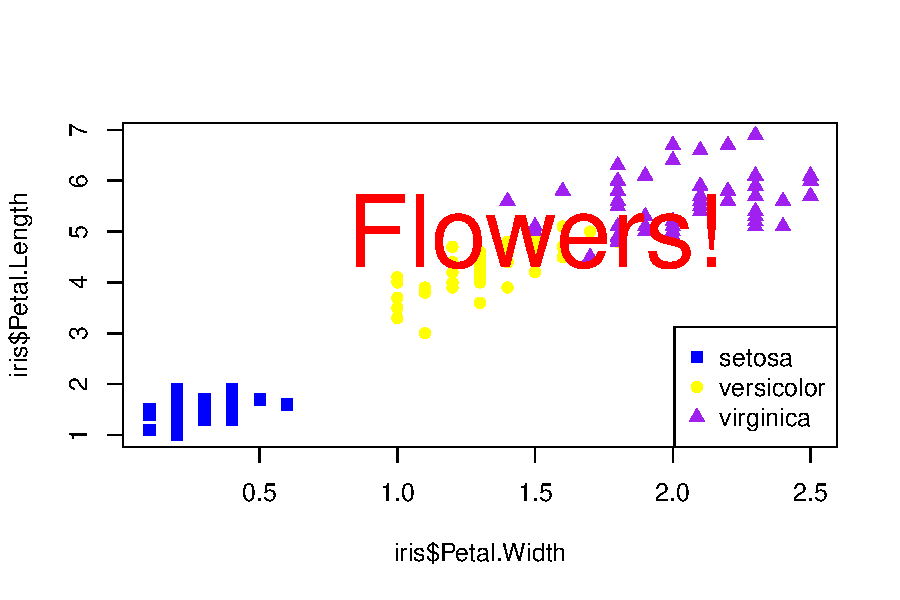
\includegraphics[keepaspectratio]{chapters/ch08_files/figure-pdf/unnamed-chunk-34-1.pdf}}

There's no way to remove the offending text: R doesn't have an ``Undo''
button! Our only option is just to remake the plot without the text.

\begin{Shaded}
\begin{Highlighting}[]
\CommentTok{\# remake without the offending text:}
\FunctionTok{plot}\NormalTok{(iris}\SpecialCharTok{$}\NormalTok{Petal.Width,iris}\SpecialCharTok{$}\NormalTok{Petal.Length,}
     \AttributeTok{pch=}\NormalTok{iris}\SpecialCharTok{$}\NormalTok{pch, }\AttributeTok{col=}\NormalTok{iris}\SpecialCharTok{$}\NormalTok{color)}
\FunctionTok{legend}\NormalTok{(}\StringTok{"bottomright"}\NormalTok{, }\AttributeTok{legend=}\NormalTok{spps, }\AttributeTok{pch=}\NormalTok{shps, }\AttributeTok{col=}\NormalTok{cols)}
\end{Highlighting}
\end{Shaded}

\pandocbounded{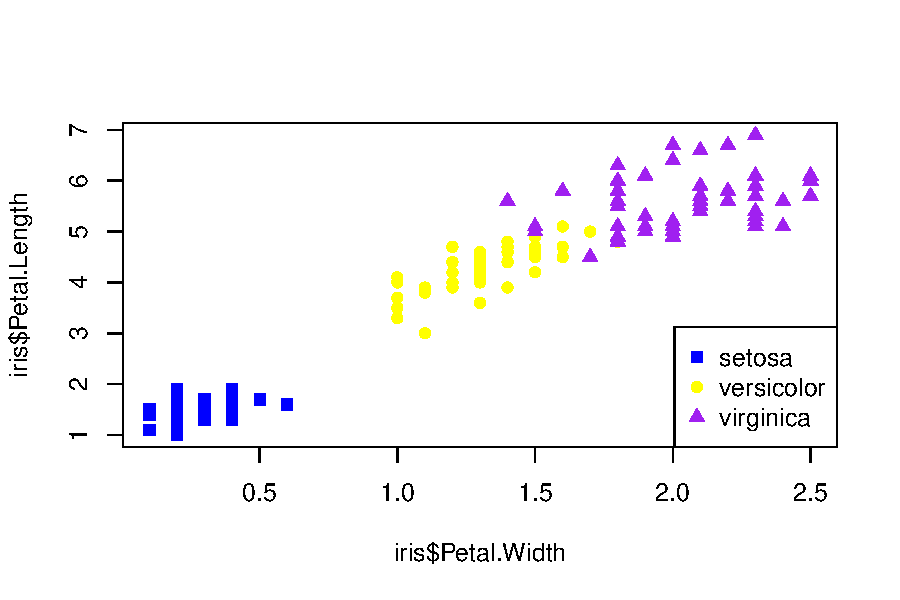
\includegraphics[keepaspectratio]{chapters/ch08_files/figure-pdf/unnamed-chunk-35-1.pdf}}

Sometimes I'll just comment out the plot component that needs deleting;
this way it is easier to add back in later. I do this a lot when I'm
trying to iteratively build a figure with lots of components.

\begin{Shaded}
\begin{Highlighting}[]
\CommentTok{\# not run:}

\CommentTok{\# remake without the offending text (commented out):}
\FunctionTok{plot}\NormalTok{(iris}\SpecialCharTok{$}\NormalTok{Petal.Width,iris}\SpecialCharTok{$}\NormalTok{Petal.Length,}
    \AttributeTok{col=}\NormalTok{use.col, }\AttributeTok{pch=}\DecValTok{16}
\NormalTok{)}
\CommentTok{\#text(1.5, 5, "Flowers!", cex=4, col="red")}
\FunctionTok{legend}\NormalTok{(}\StringTok{"bottomright"}\NormalTok{, }\AttributeTok{legend=}\NormalTok{spps, }\AttributeTok{col=}\NormalTok{cols, }\AttributeTok{pch=}\DecValTok{16}\NormalTok{)}
\end{Highlighting}
\end{Shaded}

\subsubsection{\texorpdfstring{Advanced R plotting with
\texttt{par()}}{Advanced R plotting with par()}}\label{advanced-r-plotting-with-par}

\paragraph{Plot formatting}\label{plot-formatting}

Many options that affect plots can only be set using the \texttt{par()}
function. Or, are best set using \texttt{par()}. Take a look at the
\texttt{par()} help page to get a sense of the variety of options
available (\texttt{?par}). It is important to keep in mind is that once
\texttt{par()} options are set in an R session, they will stay that way
until you change them using \texttt{par()} again. So, if you are making
multiple figures within the same R workspace or work session you will
need to pay attention to what you have done. You can always see all
current settings by running the command \texttt{par()}.

Below is an illustration of using \texttt{par()} to change graphics
options:

Without \texttt{par()}:

\begin{Shaded}
\begin{Highlighting}[]
\FunctionTok{plot}\NormalTok{(iris}\SpecialCharTok{$}\NormalTok{Petal.Length}\SpecialCharTok{\textasciitilde{}}\NormalTok{iris}\SpecialCharTok{$}\NormalTok{Sepal.Length,}
    \AttributeTok{xlab=}\StringTok{"Sepal length (cm)"}\NormalTok{,}
    \AttributeTok{ylab=}\StringTok{"Petal length (cm)"}\NormalTok{,}
     \AttributeTok{xlim=}\FunctionTok{c}\NormalTok{(}\DecValTok{0}\NormalTok{,}\DecValTok{8}\NormalTok{),}\AttributeTok{ylim=}\FunctionTok{c}\NormalTok{(}\DecValTok{0}\NormalTok{,}\DecValTok{8}\NormalTok{))}
\end{Highlighting}
\end{Shaded}

\begin{center}
\pandocbounded{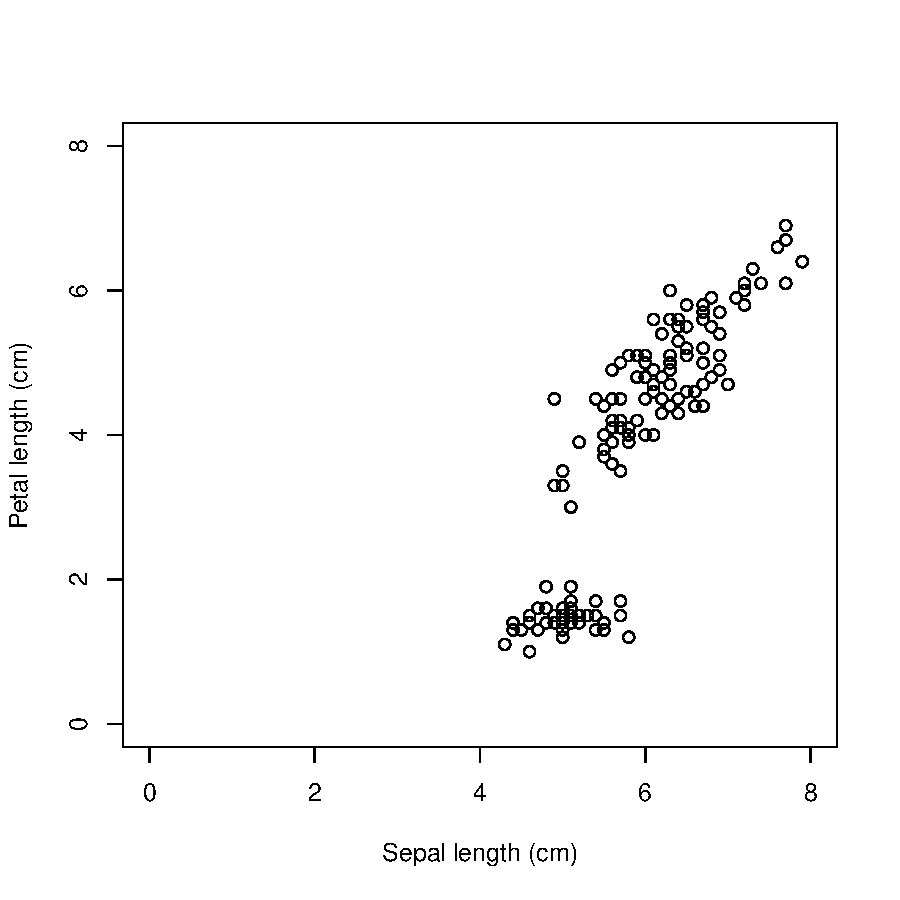
\includegraphics[keepaspectratio]{chapters/ch08_files/figure-pdf/unnamed-chunk-37-1.pdf}}
\end{center}

With \texttt{par()}, we can do the following:

\begin{itemize}
\tightlist
\item
  Narrow the margins (\texttt{mar}) so the plot takes up more of the
  figure space
\item
  Remove the box (\texttt{bty}) because it is unnecessary
\item
  Turn \emph{y}-axis numbers to horizontal (\texttt{las}) so they are
  easy to read
\item
  Bring axis labels in closer (\texttt{mgp}) to save space
\item
  Set size of axis text (\texttt{cex.axis}) and labels
  (\texttt{cex.lab}) for legibility
\end{itemize}

\begin{Shaded}
\begin{Highlighting}[]
\FunctionTok{par}\NormalTok{(}\AttributeTok{mar=}\FunctionTok{c}\NormalTok{(}\FloatTok{4.1}\NormalTok{, }\FloatTok{4.1}\NormalTok{, }\FloatTok{1.1}\NormalTok{, }\FloatTok{1.1}\NormalTok{),  }\CommentTok{\# margin sizes}
    \AttributeTok{bty=}\StringTok{"n"}\NormalTok{,                    }\CommentTok{\# no box around plot}
    \AttributeTok{las=}\DecValTok{1}\NormalTok{,                      }\CommentTok{\# axis labels in reading}
                                \CommentTok{\# direction}
    \AttributeTok{mgp=}\FunctionTok{c}\NormalTok{(}\FloatTok{2.25}\NormalTok{, }\DecValTok{1}\NormalTok{,}\DecValTok{0}\NormalTok{),           }\CommentTok{\# position of axis components}
    \AttributeTok{cex.axis=}\FloatTok{1.2}\NormalTok{,               }\CommentTok{\# size of axis numbers}
    \AttributeTok{cex.lab=}\FloatTok{1.2}\NormalTok{)                }\CommentTok{\# size of axis titles}
\FunctionTok{plot}\NormalTok{(iris}\SpecialCharTok{$}\NormalTok{Petal.Length}\SpecialCharTok{\textasciitilde{}}\NormalTok{iris}\SpecialCharTok{$}\NormalTok{Sepal.Length,}
    \AttributeTok{xlab=}\StringTok{"Sepal length (cm)"}\NormalTok{,}
    \AttributeTok{ylab=}\StringTok{"Petal length (cm)"}\NormalTok{,}
     \AttributeTok{xlim=}\FunctionTok{c}\NormalTok{(}\DecValTok{0}\NormalTok{,}\DecValTok{8}\NormalTok{),}\AttributeTok{ylim=}\FunctionTok{c}\NormalTok{(}\DecValTok{0}\NormalTok{,}\DecValTok{8}\NormalTok{))}
\end{Highlighting}
\end{Shaded}

\begin{center}
\pandocbounded{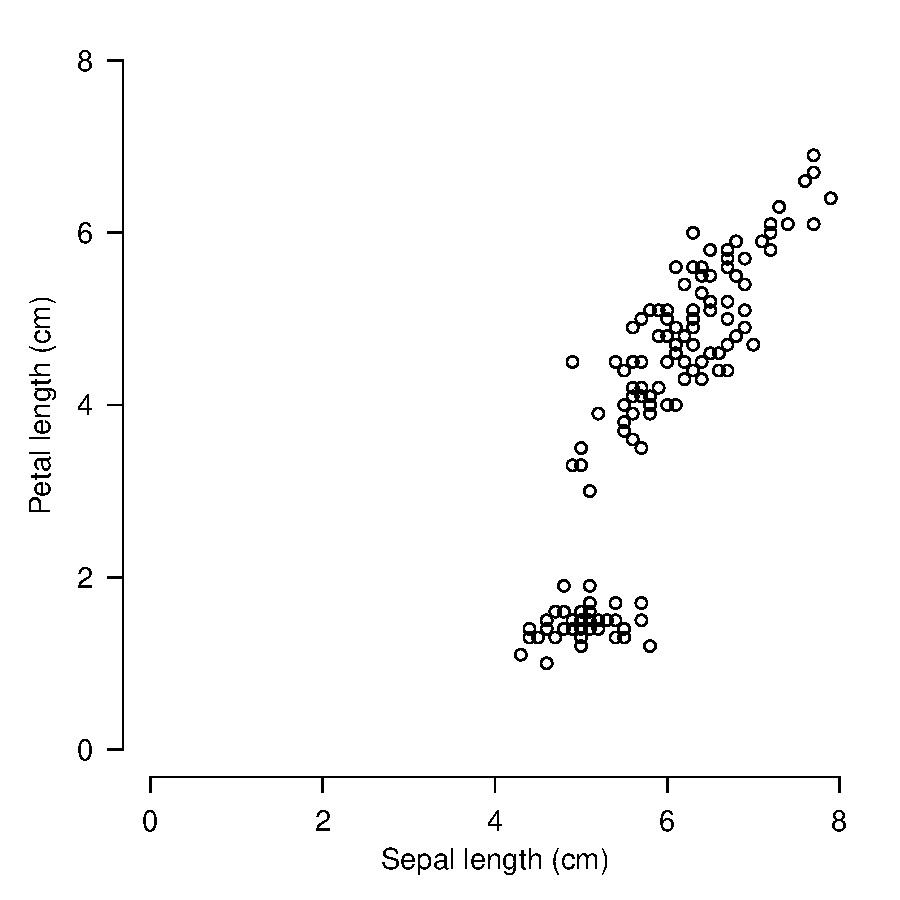
\includegraphics[keepaspectratio]{chapters/ch08_files/figure-pdf/unnamed-chunk-38-1.pdf}}
\end{center}

We will use \texttt{par()} often in this course to clean up figures and
make them more attractive. Most of the time when you are exploring data
you won't need to mess with \texttt{par()} (except for making
multi-panel figures). But, you should definitely use \texttt{par()} when
preparing figures for presentations or publications. Proper use of
\texttt{par()} is the key to making clean, informative, and
professional-looking figures.

\paragraph{\texorpdfstring{Multi-panel figures with
\texttt{par()}}{Multi-panel figures with par()}}\label{multi-panel-figures-with-par}

One of the most common ways to use \texttt{par()} is to make multi-panel
figures. The panels are specified in terms of the number of rows and
columns in the figure. The arguments \texttt{mfrow} and \texttt{mfcol}
define the panel layout.

\begin{itemize}
\tightlist
\item
  \texttt{mfrow}: you supply the number of rows and number of columns,
  in that order.
\item
  \texttt{mfcol}: works the same way, but in reverse: supply the number
  of columns and number of rows, in that order.
\end{itemize}

Once you set \texttt{mfrow} or \texttt{mfcol} (but never both), a new
plot area within the graphics window will be produced each time you call
\texttt{plot()}. The graphics window will be divided evenly according to
the number of panels you requested (e.g., \texttt{mfrow=c(2,3)} will
yield 6 panels). Panels are drawn by row and then by column (with
\texttt{mfrow}) or by column and then by row (with \texttt{mfcol}).

If you produce more plots than you have ``slots'' specified by
\texttt{mfrow} or \texttt{mfcol}, the graphics device will be cleared
and the plot panels will be filled again, in the same order as before.
So, if you set \texttt{mfrow=c(2,2)}, and then make 5 plots, you will
end up with a graphics window that has 1 plot (the fifth) in the upper
left corner.

The example below shows the use of \texttt{par()\$mfrow} to make a 2
\(\times\) 2 figure.

\begin{Shaded}
\begin{Highlighting}[]
\FunctionTok{par}\NormalTok{(}\AttributeTok{mfrow=}\FunctionTok{c}\NormalTok{(}\DecValTok{2}\NormalTok{,}\DecValTok{2}\NormalTok{),           }\CommentTok{\# layout}
    \AttributeTok{mar=}\FunctionTok{c}\NormalTok{(}\FloatTok{4.1}\NormalTok{,}\FloatTok{4.1}\NormalTok{,}\FloatTok{1.1}\NormalTok{,}\FloatTok{1.1}\NormalTok{), }\CommentTok{\# margin sizes}
    \AttributeTok{bty=}\StringTok{"n"}\NormalTok{,                }\CommentTok{\# no box around plot}
    \AttributeTok{las=}\DecValTok{1}\NormalTok{,                  }\CommentTok{\# rotate axis text}
    \AttributeTok{cex.axis=}\FloatTok{1.2}\NormalTok{,           }\CommentTok{\# axis text size}
    \AttributeTok{cex.lab=}\FloatTok{1.2}\NormalTok{)            }\CommentTok{\# label text size}
\FunctionTok{hist}\NormalTok{(iris}\SpecialCharTok{$}\NormalTok{Petal.Length, }\AttributeTok{main=}\StringTok{"Plot 1"}\NormalTok{)}
\FunctionTok{hist}\NormalTok{(iris}\SpecialCharTok{$}\NormalTok{Petal.Width, }\AttributeTok{main=}\StringTok{"Plot 2"}\NormalTok{)}
\FunctionTok{hist}\NormalTok{(iris}\SpecialCharTok{$}\NormalTok{Sepal.Length, }\AttributeTok{main=}\StringTok{"Plot 3"}\NormalTok{)}
\FunctionTok{hist}\NormalTok{(iris}\SpecialCharTok{$}\NormalTok{Sepal.Width, }\AttributeTok{main=}\StringTok{"Plot 4"}\NormalTok{)}
\end{Highlighting}
\end{Shaded}

\begin{center}
\pandocbounded{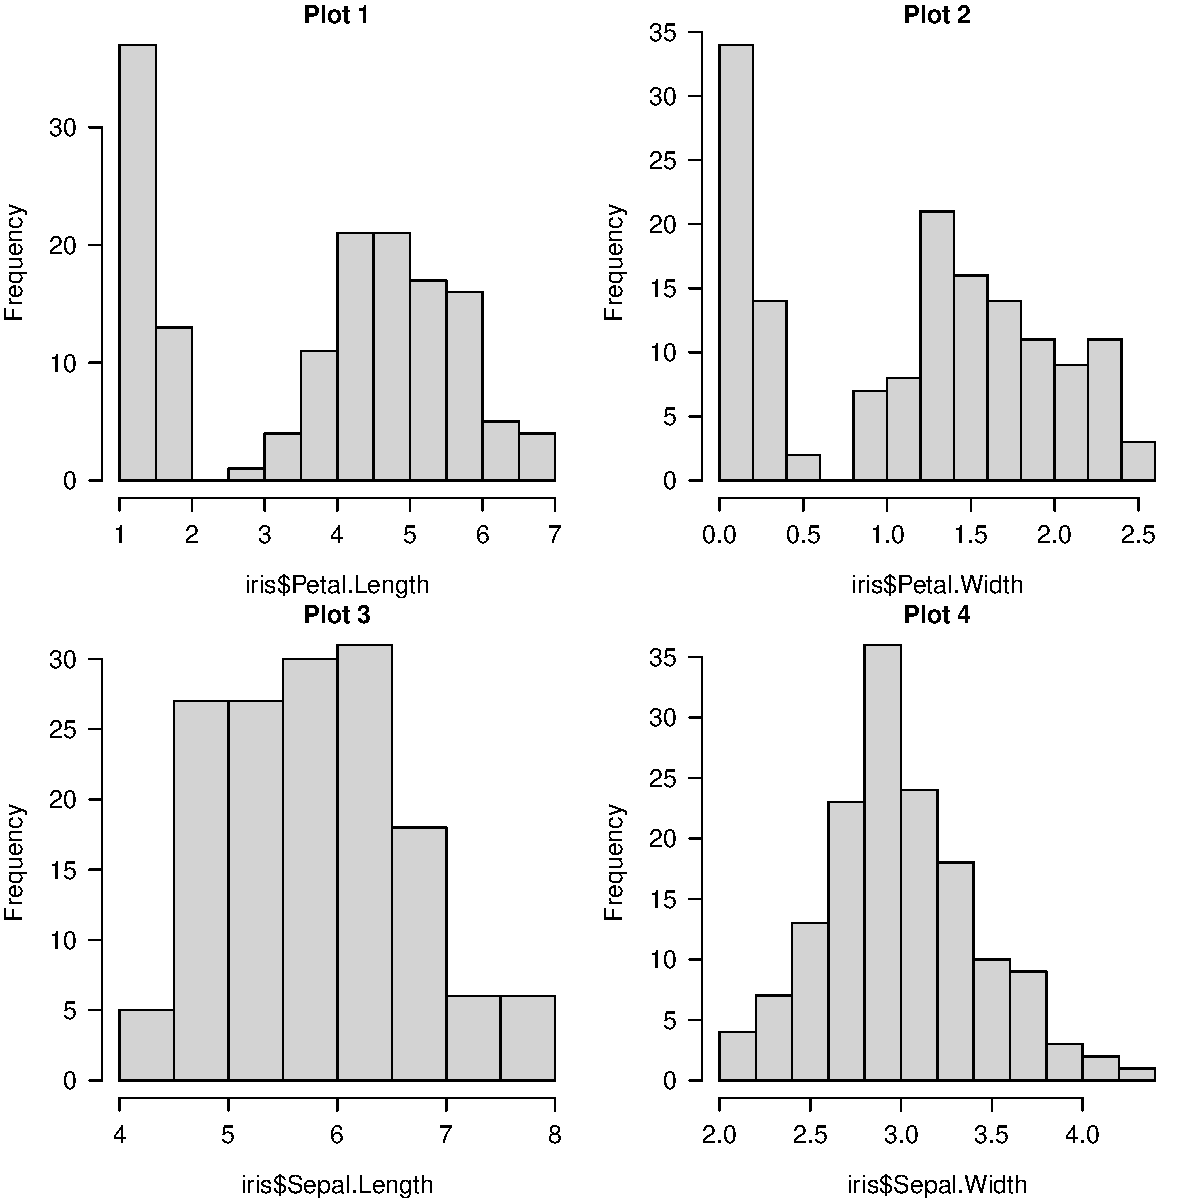
\includegraphics[keepaspectratio]{chapters/ch08_files/figure-pdf/unnamed-chunk-39-1.pdf}}
\end{center}

When making multi-panel plots, it helps to line up axes that correspond
to each other. The commands below show two separate figures with aligned
axes. This can be helpful when showing different responses to the same
explanatory variable (the 2 row by 1 column figure):

\begin{Shaded}
\begin{Highlighting}[]
\FunctionTok{par}\NormalTok{(}\AttributeTok{mfrow=}\FunctionTok{c}\NormalTok{(}\DecValTok{2}\NormalTok{,}\DecValTok{1}\NormalTok{),           }\CommentTok{\# layout}
    \AttributeTok{mar=}\FunctionTok{c}\NormalTok{(}\FloatTok{4.1}\NormalTok{,}\FloatTok{4.1}\NormalTok{,}\FloatTok{1.1}\NormalTok{,}\FloatTok{1.1}\NormalTok{), }\CommentTok{\# margin sizes}
    \AttributeTok{bty=}\StringTok{"n"}\NormalTok{,                }\CommentTok{\# no box around plot}
    \AttributeTok{las=}\DecValTok{1}\NormalTok{,                  }\CommentTok{\# rotate axis text}
    \AttributeTok{cex.axis=}\FloatTok{1.2}\NormalTok{,           }\CommentTok{\# axis text size}
    \AttributeTok{cex.lab=}\FloatTok{1.2}\NormalTok{)            }\CommentTok{\# label text size}
\FunctionTok{plot}\NormalTok{(iris}\SpecialCharTok{$}\NormalTok{Petal.Length, iris}\SpecialCharTok{$}\NormalTok{Sepal.Length)}
\FunctionTok{plot}\NormalTok{(iris}\SpecialCharTok{$}\NormalTok{Petal.Length, iris}\SpecialCharTok{$}\NormalTok{Sepal.Width)}
\end{Highlighting}
\end{Shaded}

\begin{center}
\pandocbounded{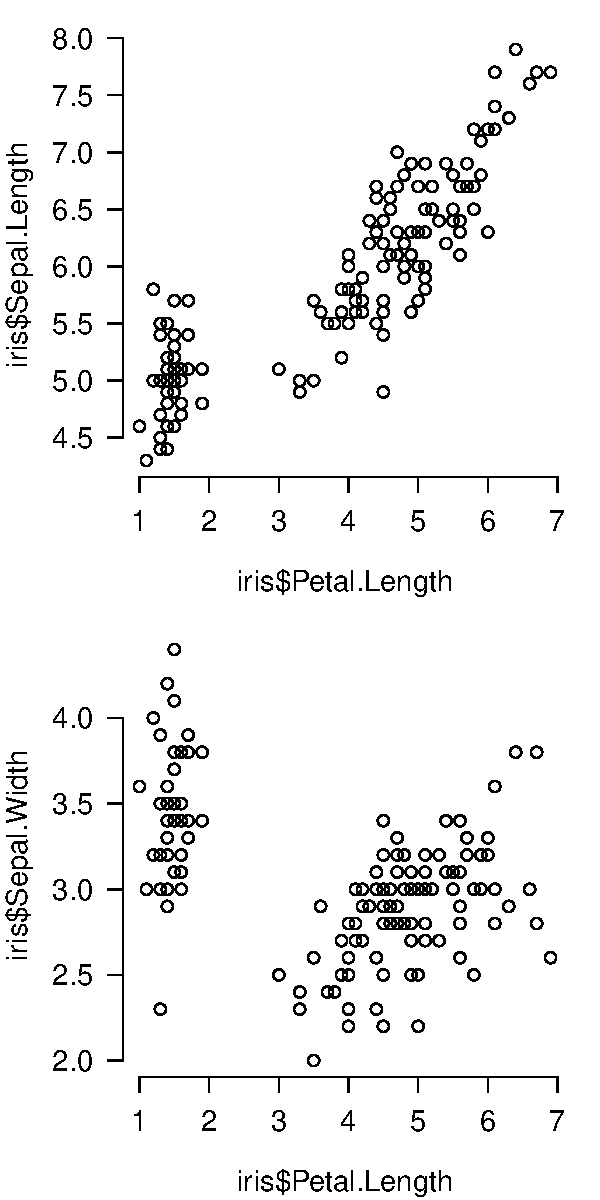
\includegraphics[keepaspectratio]{chapters/ch08_files/figure-pdf/unnamed-chunk-40-1.pdf}}
\end{center}

The figure below is a 1 row by 2 column figure that shows how a single
response variable relates to two different predictors.

\begin{Shaded}
\begin{Highlighting}[]
\FunctionTok{par}\NormalTok{(}\AttributeTok{mfrow=}\FunctionTok{c}\NormalTok{(}\DecValTok{1}\NormalTok{,}\DecValTok{2}\NormalTok{),           }\CommentTok{\# layout}
    \AttributeTok{mar=}\FunctionTok{c}\NormalTok{(}\FloatTok{4.1}\NormalTok{,}\FloatTok{4.1}\NormalTok{,}\FloatTok{1.1}\NormalTok{,}\FloatTok{1.1}\NormalTok{), }\CommentTok{\# margin sizes}
    \AttributeTok{bty=}\StringTok{"n"}\NormalTok{,                }\CommentTok{\# no box around plot}
    \AttributeTok{las=}\DecValTok{1}\NormalTok{,                  }\CommentTok{\# rotate axis text}
    \AttributeTok{cex.axis=}\DecValTok{1}\NormalTok{,           }\CommentTok{\# axis text size}
    \AttributeTok{cex.lab=}\DecValTok{1}\NormalTok{)            }\CommentTok{\# label text size}
\FunctionTok{plot}\NormalTok{(iris}\SpecialCharTok{$}\NormalTok{Petal.Width, iris}\SpecialCharTok{$}\NormalTok{Petal.Length)}
\FunctionTok{boxplot}\NormalTok{(iris}\SpecialCharTok{$}\NormalTok{Petal.Length}\SpecialCharTok{\textasciitilde{}}\NormalTok{iris}\SpecialCharTok{$}\NormalTok{Species)}
\end{Highlighting}
\end{Shaded}

\begin{center}
\pandocbounded{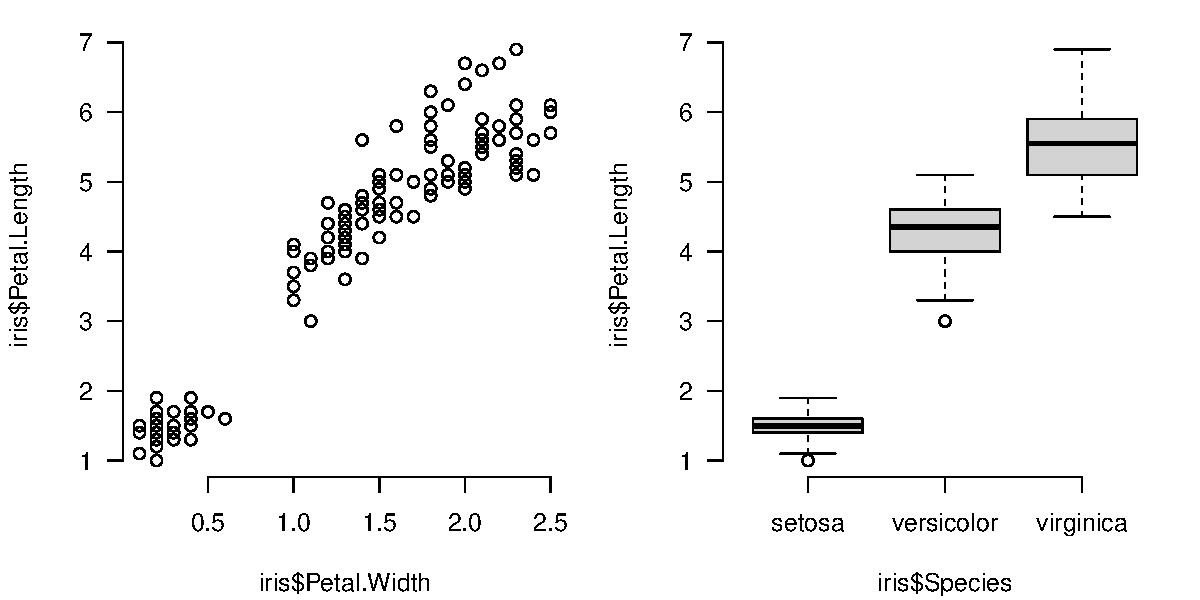
\includegraphics[keepaspectratio]{chapters/ch08_files/figure-pdf/unnamed-chunk-41-1.pdf}}
\end{center}

Sometimes you may need to manually set axis limits to make sure that the
panels line up exactly.

\begin{Shaded}
\begin{Highlighting}[]
\CommentTok{\# example with X and Y axes not aligned:}
\NormalTok{d1 }\OtherTok{\textless{}{-}}\NormalTok{ iris[}\FunctionTok{which}\NormalTok{(iris}\SpecialCharTok{$}\NormalTok{Species }\SpecialCharTok{==} \StringTok{"setosa"}\NormalTok{),]}
\NormalTok{d2 }\OtherTok{\textless{}{-}}\NormalTok{ iris[}\FunctionTok{which}\NormalTok{(iris}\SpecialCharTok{$}\NormalTok{Species }\SpecialCharTok{==} \StringTok{"versicolor"}\NormalTok{),]}

\FunctionTok{par}\NormalTok{(}\AttributeTok{mfrow=}\FunctionTok{c}\NormalTok{(}\DecValTok{2}\NormalTok{,}\DecValTok{1}\NormalTok{))}
\FunctionTok{plot}\NormalTok{(d1}\SpecialCharTok{$}\NormalTok{Petal.Length, d1}\SpecialCharTok{$}\NormalTok{Sepal.Length)}
\FunctionTok{plot}\NormalTok{(d2}\SpecialCharTok{$}\NormalTok{Petal.Length, d2}\SpecialCharTok{$}\NormalTok{Sepal.Length)}
\end{Highlighting}
\end{Shaded}

\begin{center}
\pandocbounded{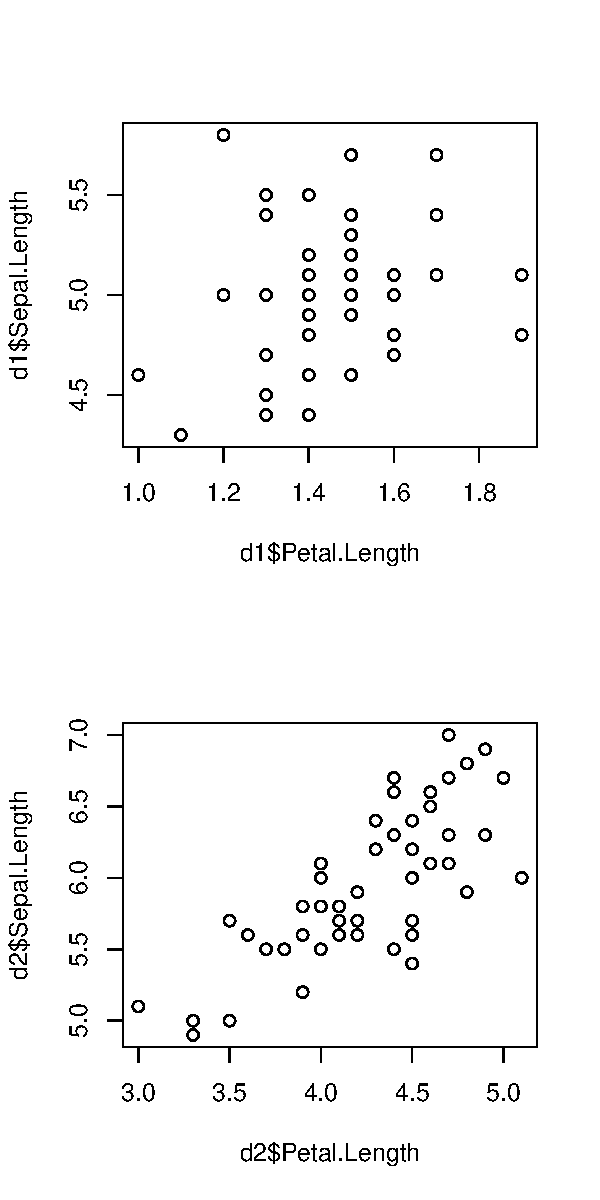
\includegraphics[keepaspectratio]{chapters/ch08_files/figure-pdf/unnamed-chunk-42-1.pdf}}
\end{center}

Here's the same plot, but with the axes lined up by setting the axis
limits with \texttt{xlim} and \texttt{ylim}.

\begin{Shaded}
\begin{Highlighting}[]
\CommentTok{\# same plot but with axes lined up:}
\FunctionTok{par}\NormalTok{(}\AttributeTok{mfrow=}\FunctionTok{c}\NormalTok{(}\DecValTok{2}\NormalTok{,}\DecValTok{1}\NormalTok{))}
\FunctionTok{plot}\NormalTok{(d1}\SpecialCharTok{$}\NormalTok{Petal.Length, d1}\SpecialCharTok{$}\NormalTok{Sepal.Length, }\AttributeTok{xlim=}\FunctionTok{c}\NormalTok{(}\DecValTok{0}\NormalTok{,}\DecValTok{6}\NormalTok{), }\AttributeTok{ylim=}\FunctionTok{c}\NormalTok{(}\DecValTok{0}\NormalTok{,}\DecValTok{8}\NormalTok{))}
\FunctionTok{plot}\NormalTok{(d2}\SpecialCharTok{$}\NormalTok{Petal.Length, d2}\SpecialCharTok{$}\NormalTok{Sepal.Length, }\AttributeTok{xlim=}\FunctionTok{c}\NormalTok{(}\DecValTok{0}\NormalTok{,}\DecValTok{6}\NormalTok{), }\AttributeTok{ylim=}\FunctionTok{c}\NormalTok{(}\DecValTok{0}\NormalTok{,}\DecValTok{8}\NormalTok{))}
\end{Highlighting}
\end{Shaded}

\begin{center}
\pandocbounded{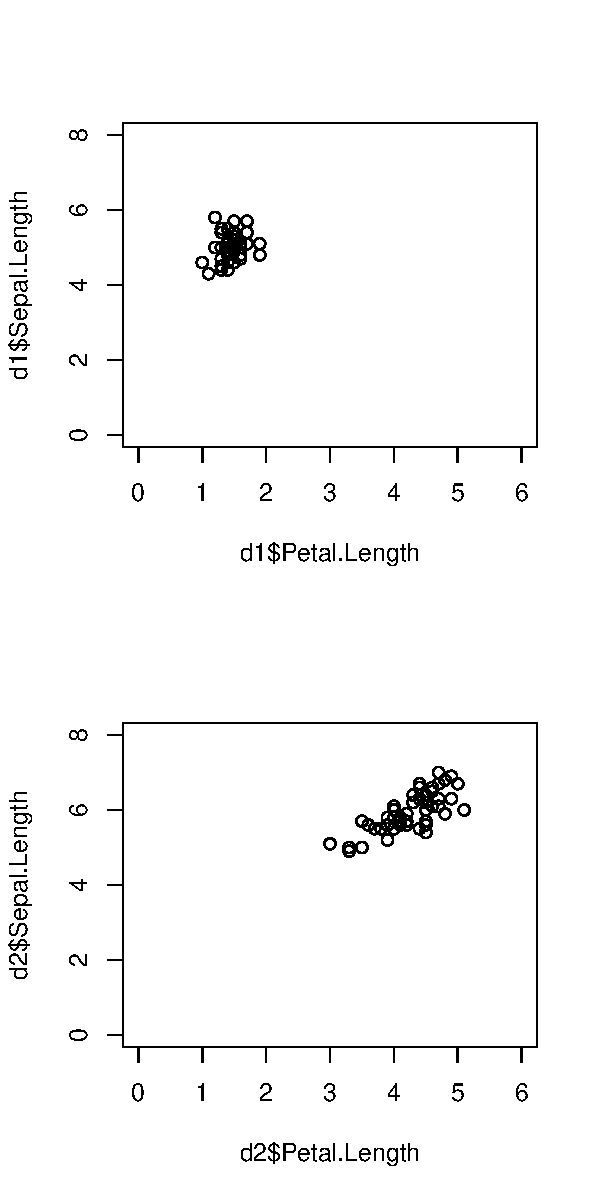
\includegraphics[keepaspectratio]{chapters/ch08_files/figure-pdf/unnamed-chunk-43-1.pdf}}
\end{center}

The argument \texttt{mfcol} to \texttt{par()} works similarly to
\texttt{mfrow}, but on columns instead of rows. For \texttt{mfcol} you
supply the number of columns, then the number of rows. Likewise, panels
are filled by column first instead of row first. The panel layout
\texttt{mfrow=c(2,3)} is the same as \texttt{mfcol=c(3,2)}, but the
panels will be filled in a different order:

\pandocbounded{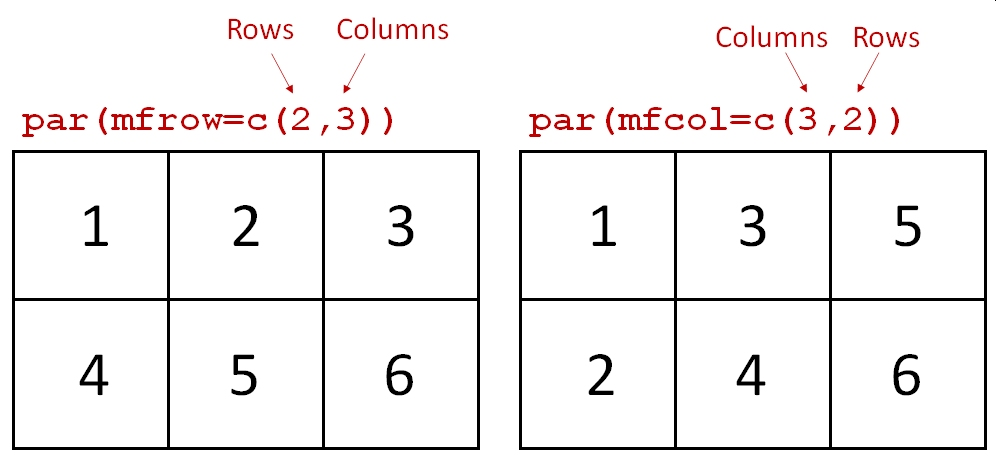
\includegraphics[keepaspectratio,alt={Illustration of how par()\$mfrow and par()\$mfcol draw and fill figure panels. mfrow fills by rows, while mfcol fills by columns.}]{chapters/../images/08-05.jpg}}\{fig-alt:
``Illustration of how par options mfrow and mfcol draw and fill figure
panels. mfrow fills by rows, while mfcol fills by columns.''\}

Whether to use \texttt{mfrow} or \texttt{mfcol} is usually a matter of
preference. Clever use of one or the other can allow you to
automatically make multi-panel plots in a preferred layout in a
\texttt{for()} loop from data stored in a list or indexed by a vector.

One last point about multi-panel plots: the \texttt{plot()} function
both creates new panels and creates plots within each panel. Part of
this process is defining the coordinate system for a panel. When you
make a plot, subsequent commands that add elements to plots such as
\texttt{points()}, \texttt{abline()}, \texttt{legend()}, etc., will use
the coordinate system of the most recent panel. Think about this when
designing complicated figures. The example below demonstrates how a
legend is placed according to the coordinate system of the most
recently-created plot.

\begin{Shaded}
\begin{Highlighting}[]
\NormalTok{n }\OtherTok{\textless{}{-}} \FloatTok{1e3}

\CommentTok{\# legend in first panel:}
\FunctionTok{par}\NormalTok{(}\AttributeTok{mfrow=}\FunctionTok{c}\NormalTok{(}\DecValTok{1}\NormalTok{,}\DecValTok{3}\NormalTok{))}
\FunctionTok{hist}\NormalTok{(}\FunctionTok{rnorm}\NormalTok{(n))}
\FunctionTok{legend}\NormalTok{(}\StringTok{"topleft"}\NormalTok{, }\AttributeTok{legend=}\StringTok{"Data"}\NormalTok{, }\AttributeTok{fill=}\StringTok{"lightgrey"}\NormalTok{)}
\FunctionTok{hist}\NormalTok{(}\FunctionTok{rnorm}\NormalTok{(n))}
\FunctionTok{hist}\NormalTok{(}\FunctionTok{rnorm}\NormalTok{(n))}
\end{Highlighting}
\end{Shaded}

\begin{center}
\pandocbounded{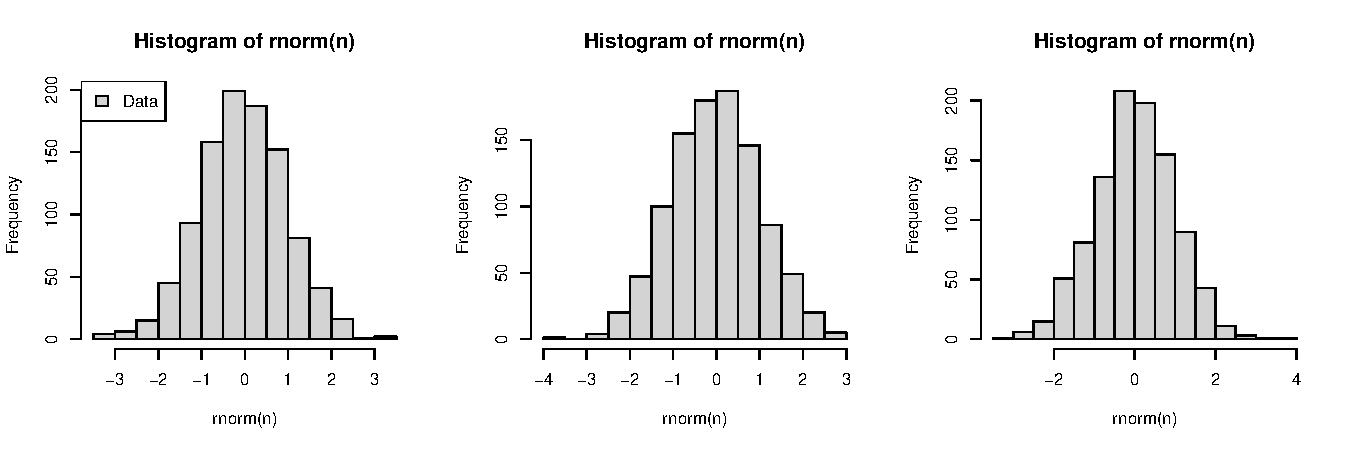
\includegraphics[keepaspectratio]{chapters/ch08_files/figure-pdf/unnamed-chunk-44-1.pdf}}
\end{center}

Here is a different figure, with the legend in a different panel:

\begin{Shaded}
\begin{Highlighting}[]
\CommentTok{\# legend in second panel (note where legend() is):}
\FunctionTok{par}\NormalTok{(}\AttributeTok{mfrow=}\FunctionTok{c}\NormalTok{(}\DecValTok{1}\NormalTok{,}\DecValTok{3}\NormalTok{))}
\FunctionTok{hist}\NormalTok{(}\FunctionTok{rnorm}\NormalTok{(n))}
\FunctionTok{hist}\NormalTok{(}\FunctionTok{rnorm}\NormalTok{(n))}
\FunctionTok{legend}\NormalTok{(}\StringTok{"topright"}\NormalTok{, }\AttributeTok{legend=}\StringTok{"Data"}\NormalTok{, }\AttributeTok{fill=}\StringTok{"lightgrey"}\NormalTok{)}
\FunctionTok{hist}\NormalTok{(}\FunctionTok{rnorm}\NormalTok{(n))}
\end{Highlighting}
\end{Shaded}

\begin{center}
\pandocbounded{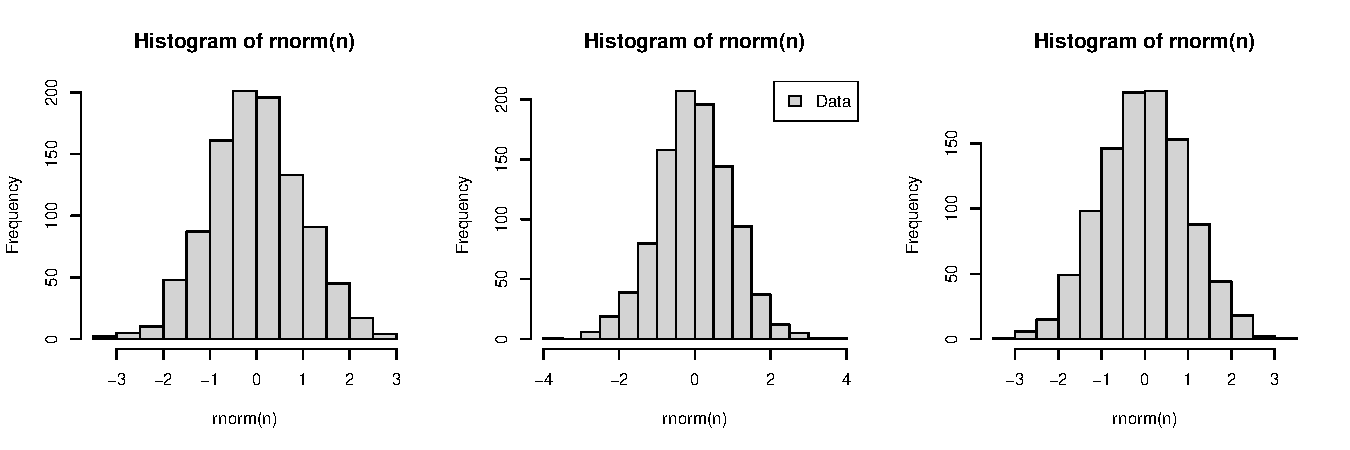
\includegraphics[keepaspectratio]{chapters/ch08_files/figure-pdf/unnamed-chunk-45-1.pdf}}
\end{center}

For more advanced plotting, refer to Chapter~\ref{sec-plot2}. There
we'll explore special symbols and equations with \texttt{plotmath()},
fun with axes, adding images to figures, and \texttt{lattice} graphics.

\section{Visualizing many variables}\label{sec-plot1-many}

\subsection{Scatterplot matrices for many
variables}\label{sec-plot1-many-pair}

\subsubsection{\texorpdfstring{Basic \texttt{pairs()}
plots}{Basic pairs() plots}}\label{basic-pairs-plots}

A scatterplot plots one variable against another, and is probably the
best way to see the relationship (if any) between two variables. But
what if you have many variables? Making dozens of scatterplots can be
tedious and time consuming. A scatterplot matrix makes many scatterplots
at once, allowing relationships between many variables to be visualized
at once. The base function to do this is \texttt{pairs()}.

\begin{Shaded}
\begin{Highlighting}[]
\CommentTok{\# load some data}
\FunctionTok{data}\NormalTok{(crabs, }\AttributeTok{package=}\StringTok{"MASS"}\NormalTok{)}

\CommentTok{\# make a spare copy}
\NormalTok{x }\OtherTok{\textless{}{-}}\NormalTok{ crabs}

\CommentTok{\# define columns for scatterplot matrix}
\NormalTok{dat.cols }\OtherTok{\textless{}{-}} \DecValTok{4}\SpecialCharTok{:}\DecValTok{8}

\CommentTok{\# make scatterplot matrix}
\FunctionTok{pairs}\NormalTok{(x[,dat.cols])}
\end{Highlighting}
\end{Shaded}

\begin{center}
\pandocbounded{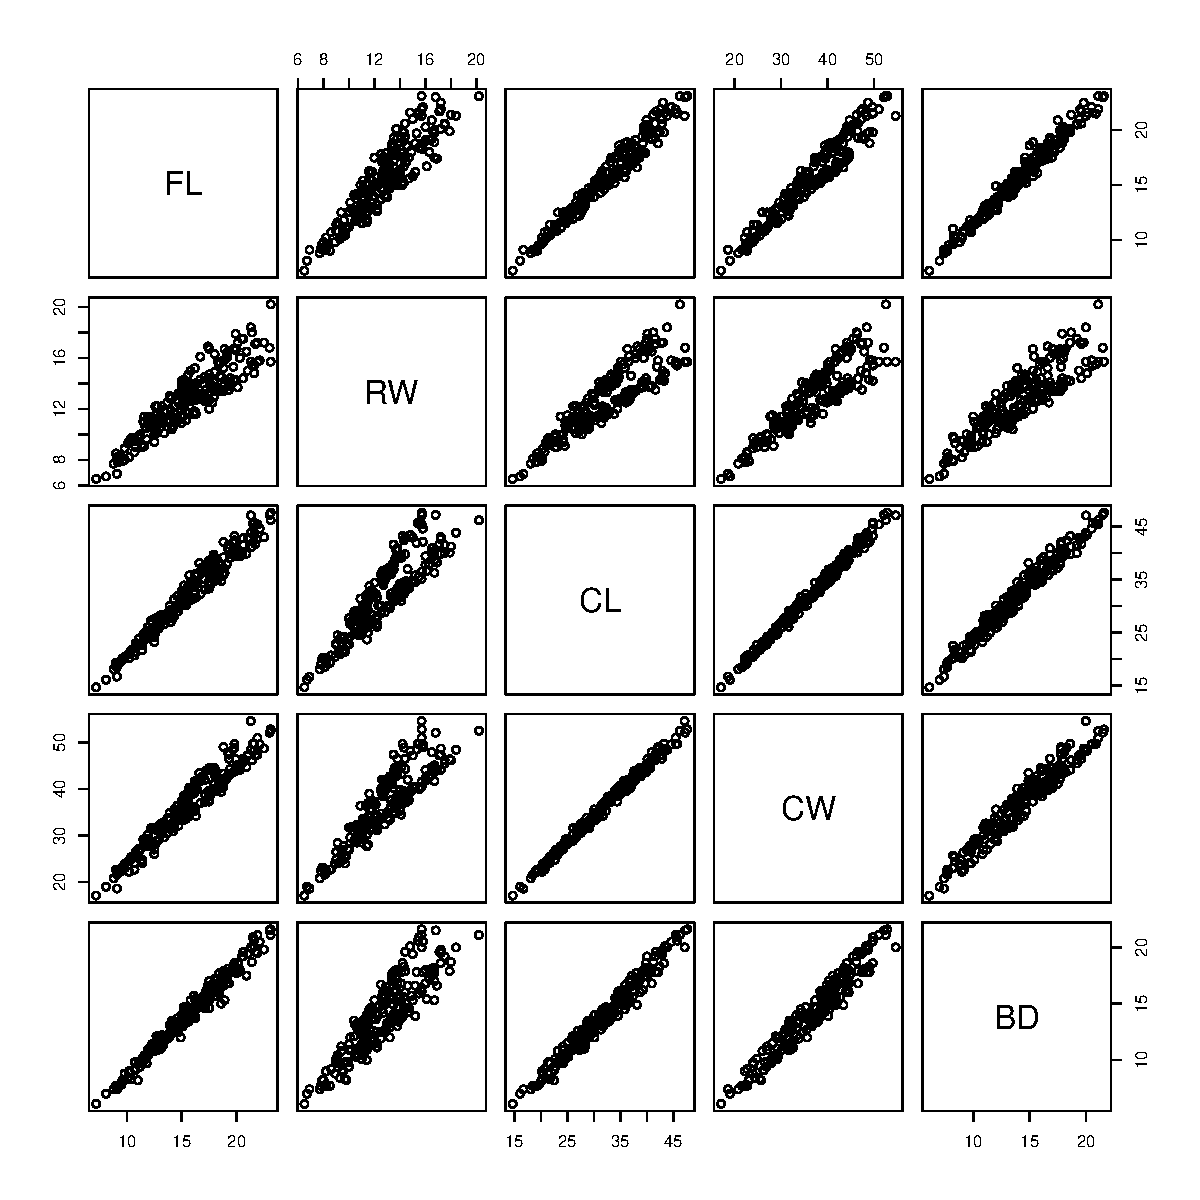
\includegraphics[keepaspectratio]{chapters/ch08_files/figure-pdf/unnamed-chunk-46-1.pdf}}
\end{center}

In the scatterplot matrix, every variable is plotted against every other
variable. Variables are labeled on the diagonal. E.g., the plots in the
first row have ``FL'' as their \emph{y}-axis, and ``RW'', ``CL'',
``CW'', and ``BD'' as their \emph{x}-axes. Likewise, plots in the first
column have ``FL'' as their \emph{x}-axis, and ``RW'', ``CL'', ``CW'',
and ``BD'' as their \emph{y}-axes.

\pandocbounded{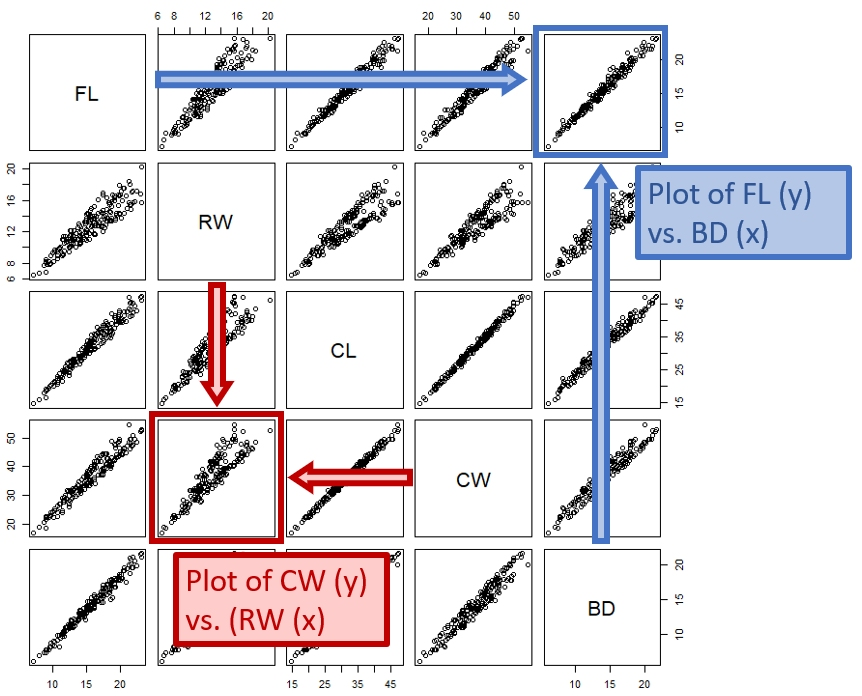
\includegraphics[keepaspectratio,alt={How to read a scatterplot matrix produced by pairs(). Each panel plots the variable in its row against the variable in its column.}]{chapters/../images/08-06.jpg}}\{Illustration
of how to read a scatterplot matrix produced by \texttt{pairs()}. Each
panel plots the variable in its row against the variable in its
column.\}

\subsubsection{\texorpdfstring{Improved \texttt{pairs()}
plots}{Improved pairs() plots}}\label{improved-pairs-plots}

One common modification to the default \texttt{pairs()} plot is to
replace scatterplots above the diagonal with correlation coefficients.
Another modification is to add linear regression or LOESS\footnote{Locally
  estimated sums of squares, a common smoothing curve algorithm.} lines
to the lower plots to help highlight the relationships. The function
below is adapted from the help page for \texttt{pairs()}. Notice that
the size of the text for each coefficient is scaled to the magnitude of
the coefficient. Can you figure out what piece of the code is doing
that?

\begin{Shaded}
\begin{Highlighting}[]
\CommentTok{\# define a function to add correlation coefficients}
\CommentTok{\# borrowed from ?pairs}
\NormalTok{panel.cor }\OtherTok{\textless{}{-}} \ControlFlowTok{function}\NormalTok{(x, y, }\AttributeTok{digits =} \DecValTok{2}\NormalTok{, }\AttributeTok{prefix =} \StringTok{""}\NormalTok{, cex.cor, ...)}
\NormalTok{\{}
    \CommentTok{\#usr \textless{}{-} par("usr"); on.exit(par(usr))}
    \FunctionTok{par}\NormalTok{(}\AttributeTok{usr =} \FunctionTok{c}\NormalTok{(}\DecValTok{0}\NormalTok{, }\DecValTok{1}\NormalTok{, }\DecValTok{0}\NormalTok{, }\DecValTok{1}\NormalTok{))}
\NormalTok{    r }\OtherTok{\textless{}{-}} \FunctionTok{cor}\NormalTok{(x, y)}
\NormalTok{    txt }\OtherTok{\textless{}{-}} \FunctionTok{format}\NormalTok{(}\FunctionTok{c}\NormalTok{(r, }\FloatTok{0.123456789}\NormalTok{), }\AttributeTok{digits =}\NormalTok{ digits)[}\DecValTok{1}\NormalTok{]}
\NormalTok{    txt }\OtherTok{\textless{}{-}} \FunctionTok{paste0}\NormalTok{(prefix, txt)}
    \ControlFlowTok{if}\NormalTok{(}\FunctionTok{missing}\NormalTok{(cex.cor)) cex.cor }\OtherTok{\textless{}{-}} \FloatTok{0.8}\SpecialCharTok{/}\FunctionTok{strwidth}\NormalTok{(txt)}
    \FunctionTok{text}\NormalTok{(}\FloatTok{0.5}\NormalTok{, }\FloatTok{0.5}\NormalTok{, txt, }\AttributeTok{cex =} \DecValTok{2}\SpecialCharTok{*}\FunctionTok{abs}\NormalTok{(r))}
\NormalTok{\}}

\CommentTok{\# example of use:}
\FunctionTok{pairs}\NormalTok{(x[,dat.cols], }
      \AttributeTok{lower.panel=}\NormalTok{panel.smooth,}
      \AttributeTok{upper.panel=}\NormalTok{panel.cor, }\AttributeTok{gap=}\DecValTok{0}\NormalTok{)}
\end{Highlighting}
\end{Shaded}

\begin{center}
\pandocbounded{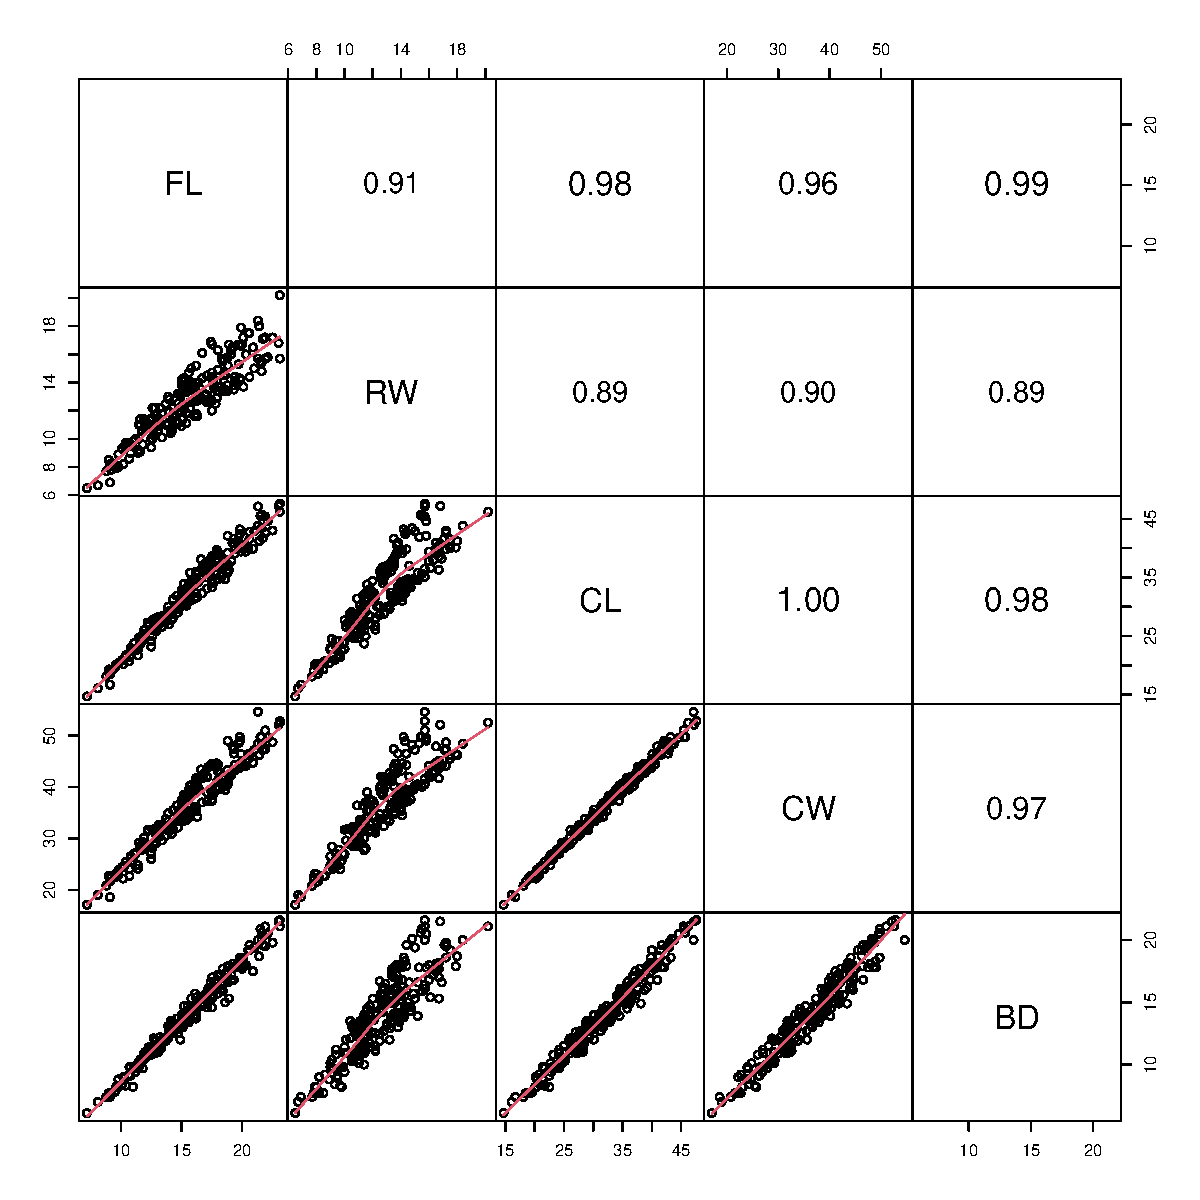
\includegraphics[keepaspectratio]{chapters/ch08_files/figure-pdf/unnamed-chunk-47-1.pdf}}
\end{center}

Sometimes the Spearman rank correlation coefficient \(\rho\) is more
informative than the Pearson linear correlation coefficient \emph{r}
(Section~\ref{sec-desc-co}). The function \texttt{panel.cor()} can be
modified to use \(\rho\) instead of \emph{r}:

\begin{Shaded}
\begin{Highlighting}[]
\NormalTok{panel.cor2 }\OtherTok{\textless{}{-}} \ControlFlowTok{function}\NormalTok{(x, y, }\AttributeTok{digits =} \DecValTok{2}\NormalTok{, }\AttributeTok{prefix =} \StringTok{""}\NormalTok{, cex.cor, ...)}
\NormalTok{\{}
    \FunctionTok{par}\NormalTok{(}\AttributeTok{usr =} \FunctionTok{c}\NormalTok{(}\DecValTok{0}\NormalTok{, }\DecValTok{1}\NormalTok{, }\DecValTok{0}\NormalTok{, }\DecValTok{1}\NormalTok{))}
\NormalTok{    r }\OtherTok{\textless{}{-}} \FunctionTok{cor}\NormalTok{(x, y, }\AttributeTok{method=}\StringTok{"spearman"}\NormalTok{)}\DocumentationTok{\#\# changed here!}
\NormalTok{    txt }\OtherTok{\textless{}{-}} \FunctionTok{format}\NormalTok{(}\FunctionTok{c}\NormalTok{(r, }\FloatTok{0.123456789}\NormalTok{), }\AttributeTok{digits =}\NormalTok{ digits)[}\DecValTok{1}\NormalTok{]}
\NormalTok{    txt }\OtherTok{\textless{}{-}} \FunctionTok{paste0}\NormalTok{(prefix, txt)}
    \ControlFlowTok{if}\NormalTok{(}\FunctionTok{missing}\NormalTok{(cex.cor)) cex.cor }\OtherTok{\textless{}{-}} \FloatTok{0.8}\SpecialCharTok{/}\FunctionTok{strwidth}\NormalTok{(txt)}
    \FunctionTok{text}\NormalTok{(}\FloatTok{0.5}\NormalTok{, }\FloatTok{0.5}\NormalTok{, txt, }\AttributeTok{cex =} \DecValTok{2}\SpecialCharTok{*}\FunctionTok{abs}\NormalTok{(r))}
\NormalTok{\}}

\CommentTok{\# example of use:}
\CommentTok{\# (might return warnings but these are ok)}
\FunctionTok{pairs}\NormalTok{(x[,dat.cols], }
      \AttributeTok{lower.panel=}\NormalTok{panel.smooth,}
      \AttributeTok{upper.panel=}\NormalTok{panel.cor2, }\AttributeTok{gap=}\DecValTok{0}\NormalTok{)}
\end{Highlighting}
\end{Shaded}

\begin{center}
\pandocbounded{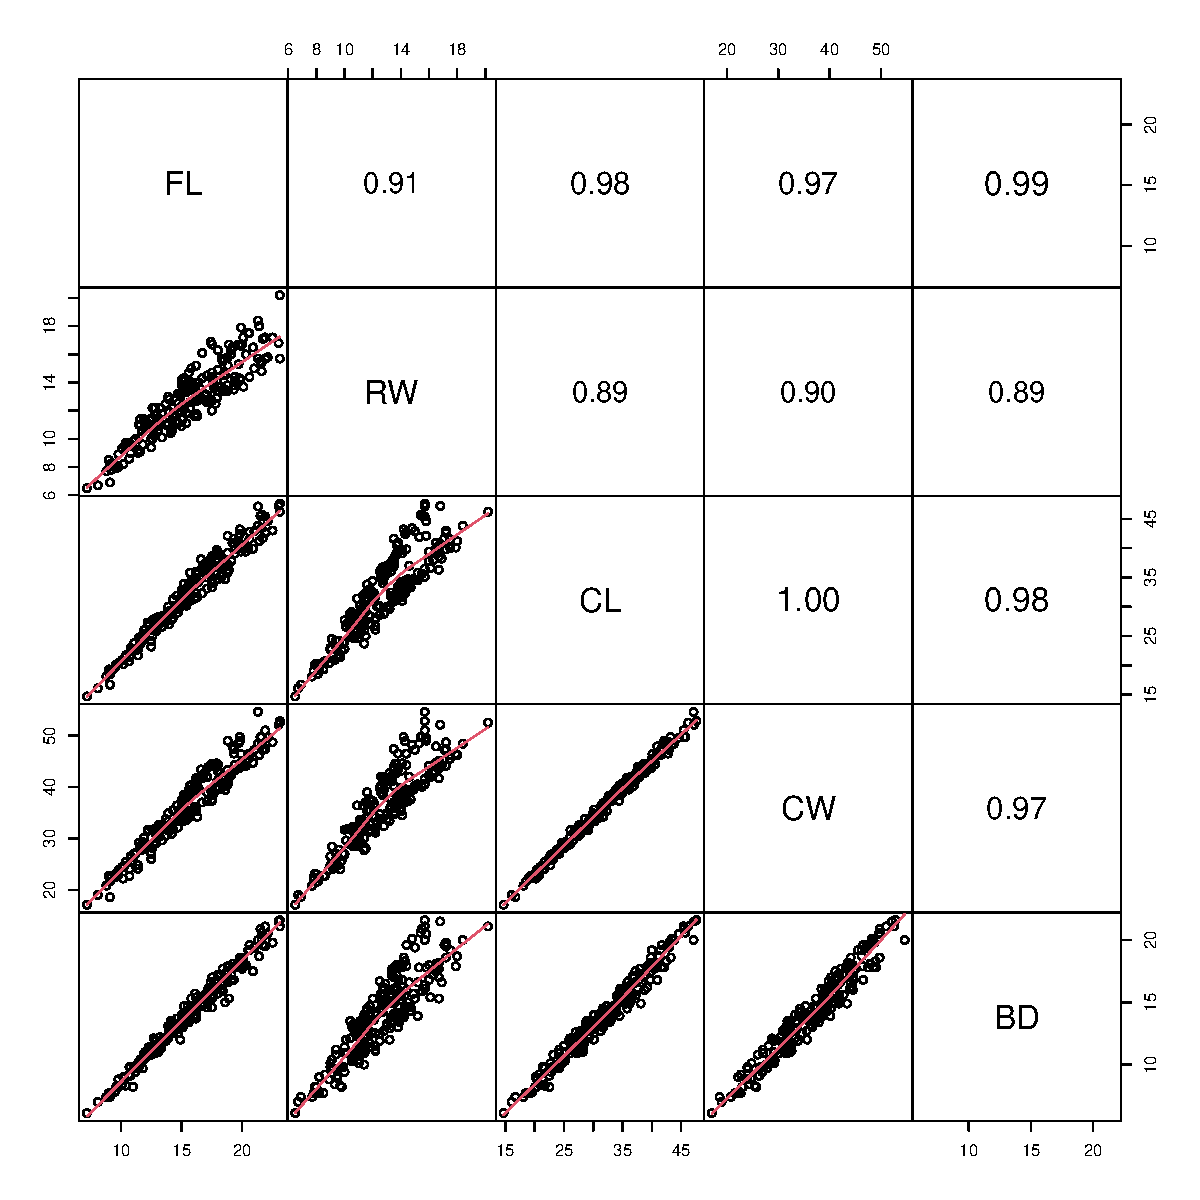
\includegraphics[keepaspectratio]{chapters/ch08_files/figure-pdf/unnamed-chunk-48-1.pdf}}
\end{center}

\subsection{Ordination (brief introduction)}\label{sec-plot1-many-ord}

The methods above are a way to examine single variables, or single pairs
of variables. But what about many variables at once? In other words, how
can we examine variation between samples by taking into account multiple
variables at once? This is the realm of \textbf{multivariate
statistics}.

\textbf{Ordination} is literally plotting or ordering observations along
two or more axes. How that ordering is done varies wildly among
techniques. We will get deeper into ordination later in the course
(Chapter~\ref{sec-ord}), but for now let's look at one of the most
common techniques, \textbf{principal components analysis (PCA)}, with a
focus on interpretation rather than calculation. Some of the goals of
all ordination techniques are:

\begin{itemize}
\tightlist
\item
  \textbf{Cluster identification:} observations that are closer to each
  other in the ordination space are more similar to each other
\item
  \textbf{Dimension reduction:} the axes of an ordination are estimates
  of synthetic variables that combine information about many variables
  at once
\end{itemize}

Biologists use many different ordination techniques to analyze patterns
in many variables at once. Regardless of the specific technique, the
basic interpretation is usually the same:

\begin{enumerate}
\def\labelenumi{\arabic{enumi}.}
\tightlist
\item
  Points that are closer together are more similar to each other.
\item
  Variables get bigger in the direction of their arrow.
\end{enumerate}

These two rules will work for almost any ordination you are likely to
encounter in biology: PCA, redundancy analysis, canonical correspondence
analysis, nonmetric multidimensional scaling (my favorite), linear
discriminant analysis, and the list goes on.

\subsubsection{Principal components analysis
(PCA)}\label{principal-components-analysis-pca}

\textbf{Principal components analysis (PCA)} is a method for extracting
synthetic gradients from a multivariate dataset that capture most of the
variation in that dataset. These gradients are calculated by finding
linear combinations of the variables that minimize sums of squared
deviations from the gradient. In other words, PCA translates the
variation between observations in terms of the original, many variables,
into variation along a few artificial variables called \textbf{principal
components}.

The basic problem is this: you can see a pattern in one variable with a
histogram (Section~\ref{sec-plot1-sing-hist}). You can see a pattern in
2 or 3 variables (i.e., dimensions) with a scatterplot
(Section~\ref{sec-plot1-two-scatter}). But what if you have 4 variables?
10 variables? If you've never heard of PCA or ordination, it might be
worth watching a video that explains and shows the basic ideas. Here is
\href{https://www.youtube.com/watch?v=HMOI_lkzW08}{\textbf{one that only
takes 5 minutes and has a nice theme song}} (accessed 2021-08-10). For a
more in-depth introduction to PCA, see \href{@sec-24-pca}{Module 24}.
For now, let's just go with ``PCA helps us visualize patterns involving
many variables at once''.

PCA is available in base R using the functions \texttt{prcomp()} and
\texttt{princomp()}. Both of these functions produce similar outputs,
but there are some subtle differences between them. For this course we
are going to use the PCA function in package \texttt{vegan}. Although
designed for community ecology, \texttt{vegan} is widely used for
ordination and multivariate analysis in many fields. Importantly,
\texttt{vegan} is actively maintained and updated with new techniques as
they are developed. Also importantly, \texttt{vegan} offers a common
interface for many kinds of ordination.

The example below uses the \texttt{varespec} dataset from
\texttt{vegan}. Each column contains \% cover by different species of
plants in lichen pastures in northern Finland and Scandinavia. For the
sake of making a simple example, we will ordinate only the 15 species
with the most variance (many species in the dataset are rare or sparse,
so including them makes the plot harder to interpret\ldots in ``real
life'', don't remove variables from your analysis without good reason!).

\begin{Shaded}
\begin{Highlighting}[]
\FunctionTok{library}\NormalTok{(vegan)}
\end{Highlighting}
\end{Shaded}

\begin{Shaded}
\begin{Highlighting}[]
\CommentTok{\# get data and make a spare copy}
\FunctionTok{data}\NormalTok{(varespec)}
\NormalTok{x }\OtherTok{\textless{}{-}}\NormalTok{ varespec}

\CommentTok{\# identify the variables with most variance}
\NormalTok{vx }\OtherTok{\textless{}{-}} \FunctionTok{rev}\NormalTok{(}\FunctionTok{sort}\NormalTok{(}\FunctionTok{apply}\NormalTok{(x, }\DecValTok{2}\NormalTok{, var)))}
\NormalTok{x }\OtherTok{\textless{}{-}}\NormalTok{ x[,}\FunctionTok{names}\NormalTok{(vx)[}\DecValTok{1}\SpecialCharTok{:}\DecValTok{10}\NormalTok{]]}

\CommentTok{\# calculate PCA and plot it}
\NormalTok{p1 }\OtherTok{\textless{}{-}} \FunctionTok{pca}\NormalTok{(x, }\AttributeTok{scale=}\ConstantTok{TRUE}\NormalTok{)}
\FunctionTok{biplot}\NormalTok{(p1)}
\end{Highlighting}
\end{Shaded}

\begin{center}
\pandocbounded{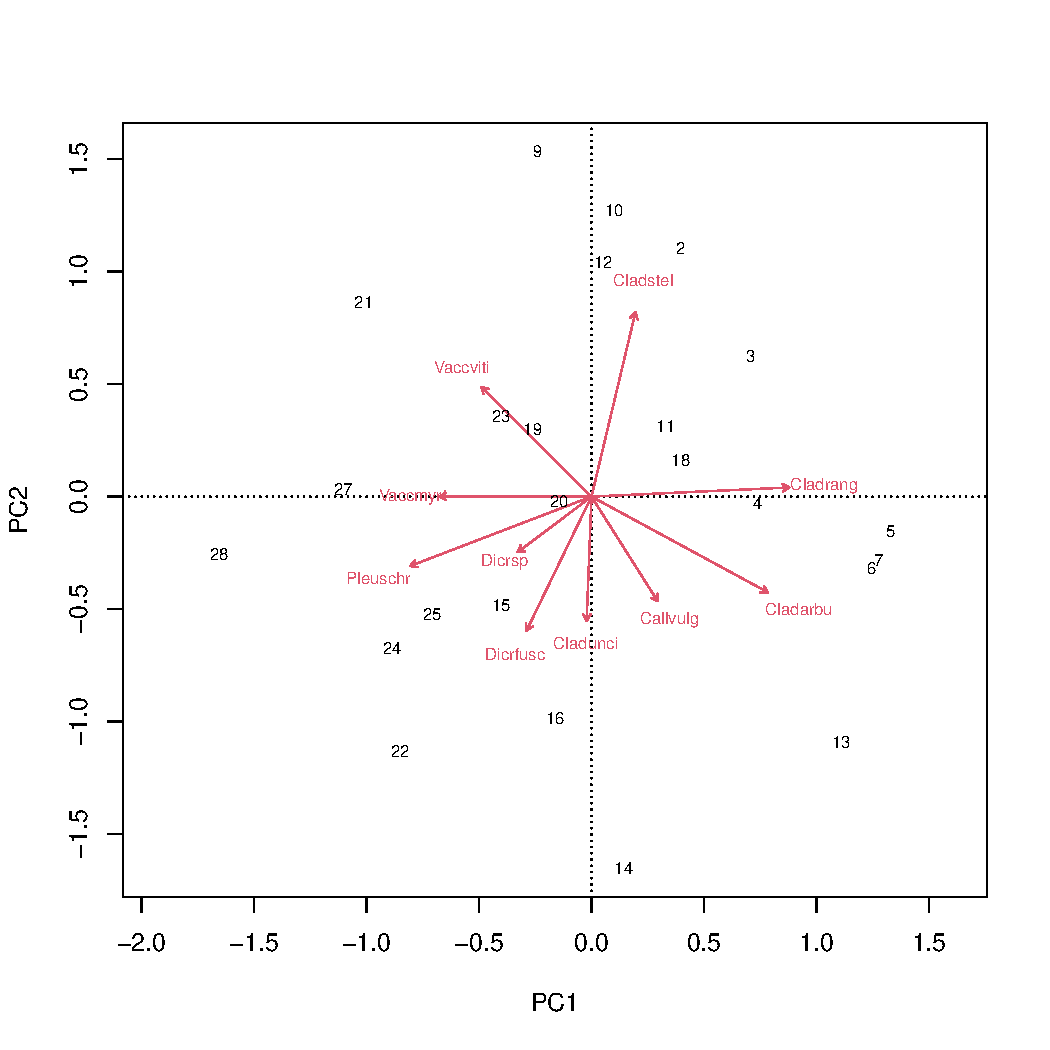
\includegraphics[keepaspectratio]{chapters/ch08_files/figure-pdf/unnamed-chunk-50-1.pdf}}
\end{center}

The figure above is called a \textbf{PCA biplot}. Each point is a sample
(site) where vegetation was sampled. By default, the samples are
identified by their row number. The red arrows show sites where
different species were more abundant (or, more generally, where the
variables are increasing). For example, sites towards the top right had
greater cover by species ``Cladstel''. Sites towards the lower left had
less cover by Cladstel. Sites towards the top left had more cover by
``Pleuschr''.

The \texttt{summary()} command will print a lot of information about the
ordination. It prints the eigenvalues of each PC, then scales them as
``Proportion explained''. I.e., the proportion of variation explained by
each PC is the same as its eigenvalue divided by the sum of all
eigenvalues.

\begin{Shaded}
\begin{Highlighting}[]
\FunctionTok{summary}\NormalTok{(p1)}
\end{Highlighting}
\end{Shaded}

\begin{verbatim}

Call:
pca(X = x, scale = TRUE) 

Partitioning of correlations:
              Inertia Proportion
Total              10          1
Unconstrained      10          1

Eigenvalues, and their contribution to the correlations 

Importance of components:
                         PC1    PC2    PC3    PC4     PC5    PC6     PC7
Eigenvalue            2.7808 1.9382 1.3148 1.0987 0.83622 0.7150 0.69134
Proportion Explained  0.2781 0.1938 0.1315 0.1099 0.08362 0.0715 0.06913
Cumulative Proportion 0.2781 0.4719 0.6034 0.7132 0.79687 0.8684 0.93750
                          PC8     PC9    PC10
Eigenvalue            0.33428 0.17151 0.11919
Proportion Explained  0.03343 0.01715 0.01192
Cumulative Proportion 0.97093 0.98808 1.00000
\end{verbatim}

The ``Importance of components'' part tells us that the first principal
component (PC1) explains about 27.8\% of the variation in the dataset.
PC2 explains an additional 19.4\%. One rule of thumb people use is to
present enough PCs to account for \(\ge{80\%}\) of the variation. If it
takes many PCs to reach 80\% of variation, that may be a sign that the
PCs are not capturing much meaningful structure in your dataset (or,
there simply isn't much structure to capture).

Finally, we can see the variable \textbf{loadings}, which describe the
contribution of each original variable to each principal
component\footnote{Different software packages define loadings slightly
  differently. Some report the coefficients (eigenvectors) used to
  calculate the principal components, while others report the
  correlations between the original variables and the principal
  components. The two are closely related and usually lead to the same
  qualitative interpretation. We'll discuss this more in
  Chapter~\ref{sec-ord}.}. Loadings with larger absolute values indicate
variables that contribute more strongly to an axis, while the sign
indicates the direction of that relationship. In the example below,
unscaled loadings for PCs 1-4 are requested using \texttt{choices=1:4}
and \texttt{scaling=0}.

\begin{Shaded}
\begin{Highlighting}[]
\FunctionTok{scores}\NormalTok{(p1, }\AttributeTok{choices =} \DecValTok{1}\SpecialCharTok{:}\DecValTok{4}\NormalTok{, }\AttributeTok{display =} \StringTok{"species"}\NormalTok{, }\AttributeTok{scaling =} \DecValTok{0}\NormalTok{)}
\end{Highlighting}
\end{Shaded}

\begin{verbatim}
                PC1           PC2         PC3        PC4
Cladstel  0.1118986  0.5621722123 -0.14606363  0.4467186
Pleuschr -0.4612677 -0.2115389675  0.17670529 -0.2214946
Cladrang  0.5037497  0.0279351716  0.18537465 -0.3339431
Cladarbu  0.4490762 -0.2918262462  0.08645467 -0.3032787
Dicrfusc -0.1655069 -0.4091013432  0.12191016  0.4270946
Vaccviti -0.2801468  0.3347151730 -0.09280300 -0.1347303
Dicrsp   -0.1879928 -0.1693471498 -0.57673161 -0.2878989
Callvulg  0.1685866 -0.3191415425  0.21724150  0.4741263
Cladunci -0.0123003 -0.3786062372 -0.50705444  0.1445745
Vaccmyrt -0.3866379  0.0003420561  0.49518742 -0.1368990
attr(,"const")
[1] 3.894323
\end{verbatim}

The loadings indicate that PC1 is strongly associated with species
\texttt{Cladrang} and, to a lesser extent, \texttt{Pleuschr}. The signs
of the loadings indicate whether the species vary in the positive or
negative direction along PC1. Compare this to the orientation and length
of the corresponding arrow in the biplot. Variables with larger absolute
loadings generally have longer arrows and exert a stronger influence on
the principal component.

\subsubsection{Plotting ordinations}\label{plotting-ordinations}

Extracting the scores from an ordination object can let you plot points
with all of the \texttt{base} graphics formatting methods we learned
above (Section~\ref{sec-plot1-two}), such as using color or shape to
indicate group membership. In my experience this is more flexible than
using the built-in graphics capabilities in \texttt{vegan}\footnote{An
  introduction by the package's lead author can be found by running this
  command:\texttt{vignette(topic="intro-vegan",\ package="vegan")}.},
but your mileage may vary.

\begin{Shaded}
\begin{Highlighting}[]
\CommentTok{\# load some data}
\FunctionTok{data}\NormalTok{(crabs, }\AttributeTok{package=}\StringTok{"MASS"}\NormalTok{)}

\CommentTok{\# make a spare copy}
\NormalTok{x }\OtherTok{\textless{}{-}}\NormalTok{ crabs}

\CommentTok{\# fit the PCA on the numerical variables}
\NormalTok{p1 }\OtherTok{\textless{}{-}} \FunctionTok{pca}\NormalTok{(x[,}\DecValTok{4}\SpecialCharTok{:}\DecValTok{8}\NormalTok{], }\AttributeTok{scale=}\ConstantTok{TRUE}\NormalTok{)}

\CommentTok{\# extract the "scores": coordinates on PC axes}
\NormalTok{site.scores }\OtherTok{\textless{}{-}} \FunctionTok{scores}\NormalTok{(p1, }\AttributeTok{choices=}\DecValTok{1}\SpecialCharTok{:}\DecValTok{2}\NormalTok{,}
                      \AttributeTok{display=}\StringTok{"sites"}\NormalTok{, }\AttributeTok{scaling=}\StringTok{"sites"}\NormalTok{)}

\CommentTok{\# define some colors for sex}
\NormalTok{use.colors }\OtherTok{\textless{}{-}} \FunctionTok{c}\NormalTok{(}\StringTok{"red"}\NormalTok{, }\StringTok{"blue"}\NormalTok{)}
\FunctionTok{names}\NormalTok{(use.colors) }\OtherTok{\textless{}{-}} \FunctionTok{sort}\NormalTok{(}\FunctionTok{unique}\NormalTok{(x}\SpecialCharTok{$}\NormalTok{sex))}
\NormalTok{x}\SpecialCharTok{$}\NormalTok{color }\OtherTok{\textless{}{-}}\NormalTok{ use.colors[x}\SpecialCharTok{$}\NormalTok{sex]}

\CommentTok{\# define some shapes for species}
\NormalTok{use.pch }\OtherTok{\textless{}{-}} \FunctionTok{c}\NormalTok{(}\DecValTok{2}\NormalTok{,}\DecValTok{1}\NormalTok{)}
\FunctionTok{names}\NormalTok{(use.pch) }\OtherTok{\textless{}{-}} \FunctionTok{sort}\NormalTok{(}\FunctionTok{unique}\NormalTok{(x}\SpecialCharTok{$}\NormalTok{sp))}
\NormalTok{x}\SpecialCharTok{$}\NormalTok{pch }\OtherTok{\textless{}{-}}\NormalTok{ use.pch[x}\SpecialCharTok{$}\NormalTok{sp]}

\CommentTok{\# build the plot}
\FunctionTok{par}\NormalTok{(}\AttributeTok{mfrow=}\FunctionTok{c}\NormalTok{(}\DecValTok{1}\NormalTok{,}\DecValTok{1}\NormalTok{))}
\FunctionTok{plot}\NormalTok{(site.scores, }\AttributeTok{col=}\NormalTok{x}\SpecialCharTok{$}\NormalTok{color, }\AttributeTok{pch=}\NormalTok{x}\SpecialCharTok{$}\NormalTok{pch,}
     \AttributeTok{xlab=}\StringTok{"PC1 (95.8\%)"}\NormalTok{, }\AttributeTok{ylab=}\StringTok{"PC2 (3.0\%)"}\NormalTok{)}
\FunctionTok{legend}\NormalTok{(}\StringTok{"topleft"}\NormalTok{,}
       \AttributeTok{legend=}\FunctionTok{c}\NormalTok{(}\StringTok{"B female"}\NormalTok{, }\StringTok{"B male"}\NormalTok{, }\StringTok{"O female"}\NormalTok{, }\StringTok{"O male"}\NormalTok{),}
       \AttributeTok{pch=}\FunctionTok{c}\NormalTok{(}\DecValTok{2}\NormalTok{, }\DecValTok{2}\NormalTok{, }\DecValTok{1}\NormalTok{, }\DecValTok{1}\NormalTok{),}
       \AttributeTok{col=}\FunctionTok{c}\NormalTok{(}\StringTok{"red"}\NormalTok{, }\StringTok{"blue"}\NormalTok{, }\StringTok{"red"}\NormalTok{, }\StringTok{"blue"}\NormalTok{))}
\end{Highlighting}
\end{Shaded}

\begin{center}
\pandocbounded{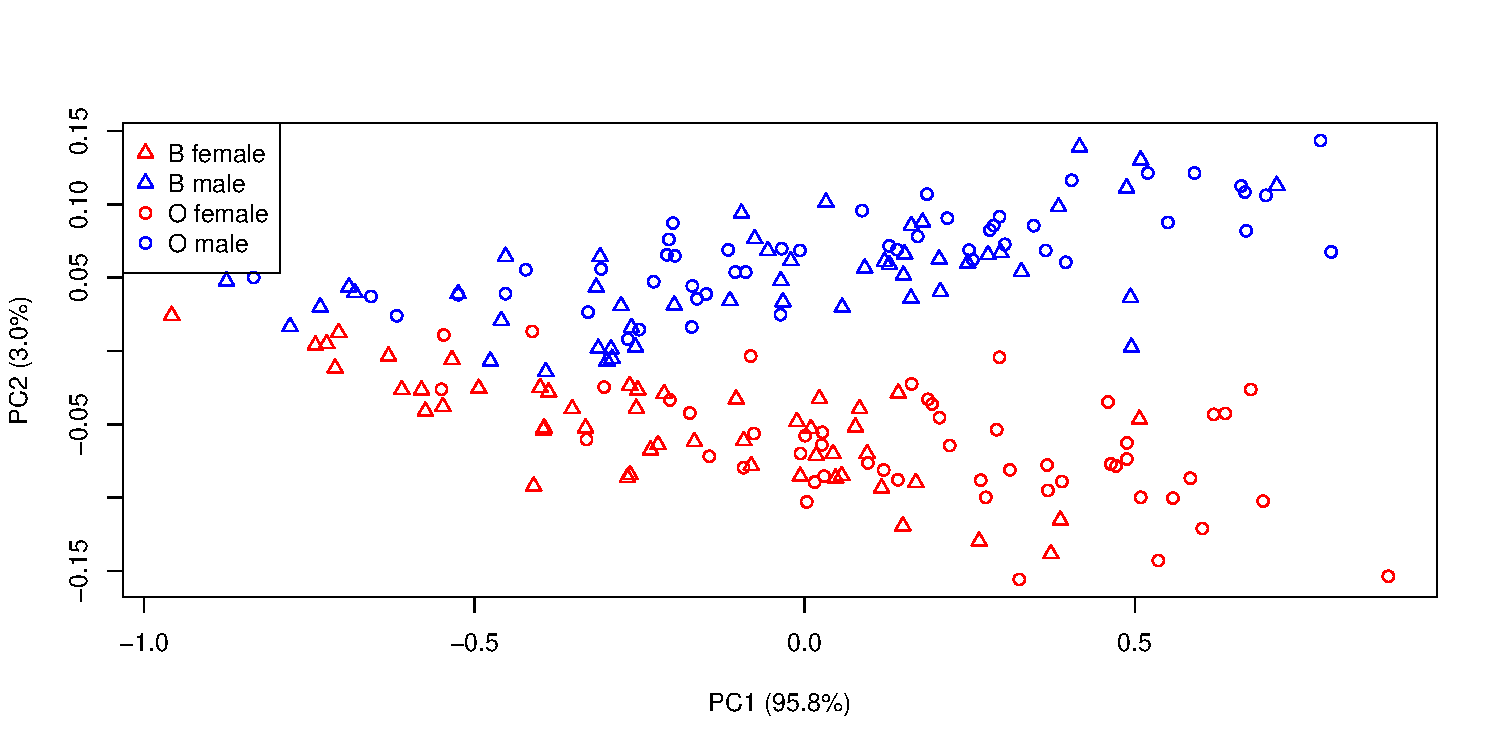
\includegraphics[keepaspectratio]{chapters/ch08_files/figure-pdf/unnamed-chunk-53-1.pdf}}
\end{center}

Some interpretations of this plot:

\begin{enumerate}
\def\labelenumi{\arabic{enumi}.}
\tightlist
\item
  Almost all of the variance is on PC1. Because the underlying data are
  measurements, and measurements are often correlated with overall size,
  PC1 is probably a gradient of overall body size. If we wanted to use
  PCA to capture shape variation, we would need to factor out overall
  size first somehow. Or, not interpret PC1.
\item
  The species B and O (triangles and circles) do not appear to be well
  distinguished by either PC1 or PC2.
\item
  The sexes (red and blue) are well separated by PC2, with females
  having smaller values and males having greater values.
\end{enumerate}

\subsubsection{Ordination wrap-up (for
now)}\label{ordination-wrap-up-for-now}

Ordination is a collection of methods for reducing the dimensionality of
data. Biological datasets often have many variables, but most variation
in those datasets can often be captured using only a few of them (or few
combinations of the variables). The positions of the samples in the
ordination space can thus reveal patterns that are too complicated to
see in the full data space. Interpreting ordination axes in biological
terms can be very fruitful. When an axis captures important information
about the samples, it can be used as a variable in another method (e.g.,
as a predictor variable in a linear model). Analysis of clustering or
positional differences between groups in ordination space (especially
NMDS space) can allow for researchers to test for differences in many
variables at once.

\chapter{Probability distributions for biologists}\label{sec-dist}

\section{Introduction}\label{sec-dist-intro}

All data contain some element of randomness. Understanding the nature
and consequences of that randomness is what motivates much of modern
statistics. \textbf{Probability distributions} are the mathematical
constructs that describe randomness in data. This module describes some
probability distributions commonly encountered in biology (and a few
that aren't common). The emphasis here is on practical understanding of
what the distributions imply about data--not on the theoretical
underpinnings or mathematical details. If you want or need a rigorous
introduction to probability theory, this is probably not the right
place.

\subsection{Residuals: the random variation left
over}\label{residuals-the-random-variation-left-over}

Consider the figures below:

\begin{center}
\pandocbounded{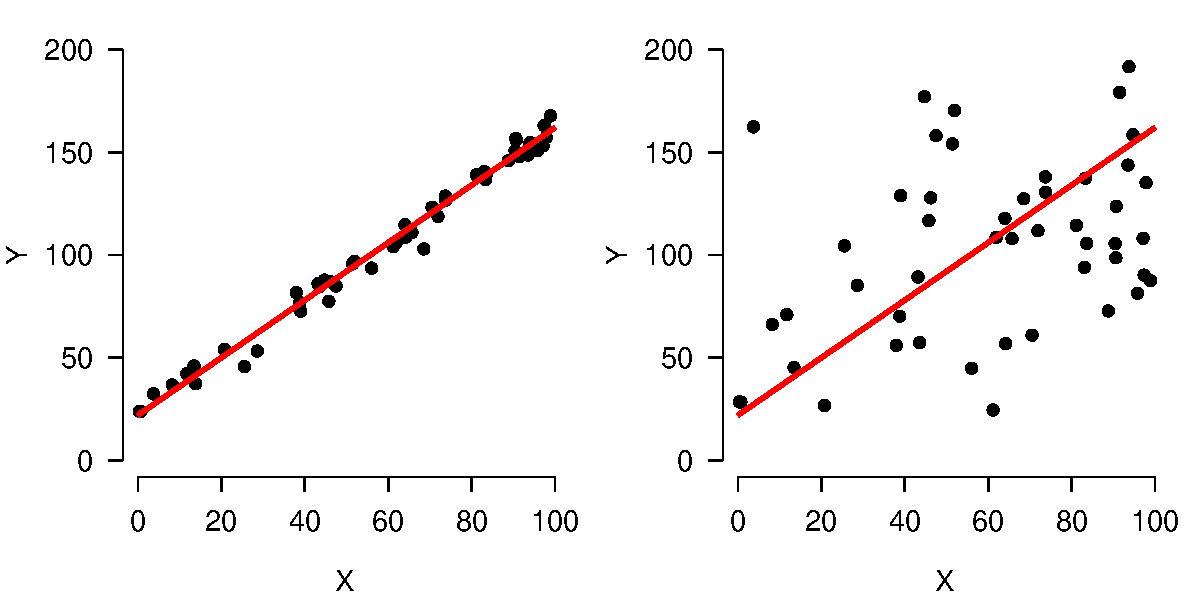
\includegraphics[keepaspectratio]{chapters/ch09_files/figure-pdf/unnamed-chunk-1-1.pdf}}
\end{center}

Both scatterplots show a linear relationship between \emph{X} and
\emph{Y}. But what is different about the plot on the right? Variation.
Both plots show the same relationship (\(Y=22+1.4X\)), but they differ
in that the variation about the expected value (the red line) is much
greater in the right plot than the left plot. Consequently, \emph{X}
appears to explain much more variation in \emph{Y} in the left plot than
in the right plot. The next figure shows that the \textbf{residual
variation}, or difference between the expected and observed values, is
much greater in the right panel. Each of these differences between the
observed value of \emph{Y} (\(Y_i\)) and the expected value of \emph{Y}
(\(E(Y_i)\)), or \(Y_i-E(Y_i)\), is called a \textbf{residual}.

\begin{center}
\pandocbounded{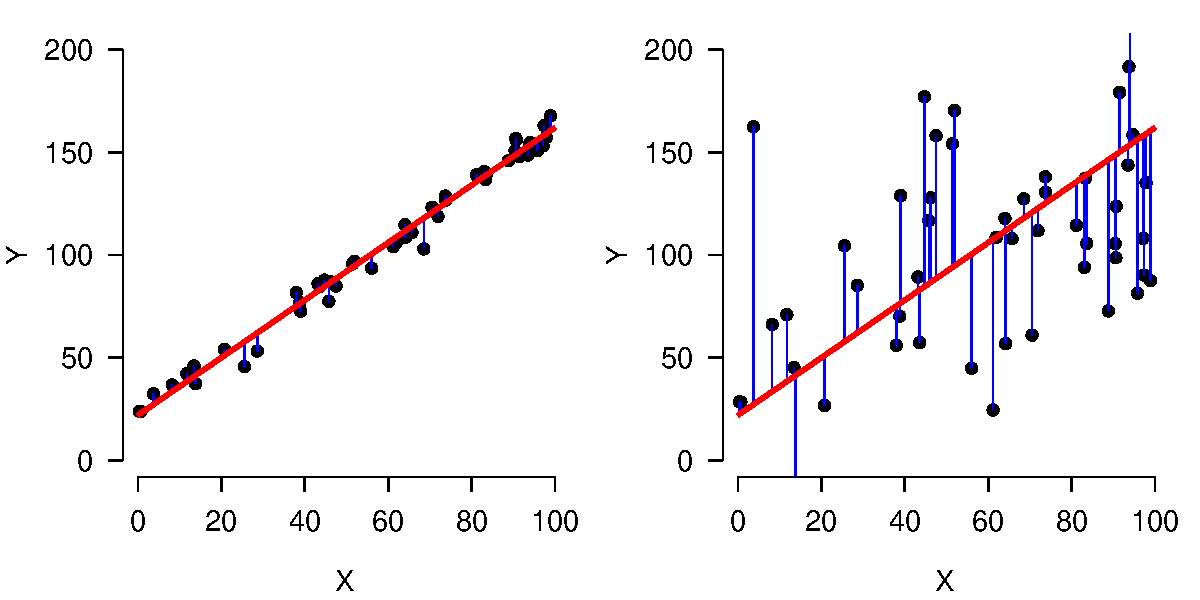
\includegraphics[keepaspectratio]{chapters/ch09_files/figure-pdf/unnamed-chunk-2-1.pdf}}
\end{center}

Residuals are an important part of statistical analysis for two reasons.
First, most statistical models make assumptions about the distribution
of residuals. Second, the total magnitude of the residuals (usually
expressed as sum of squared residuals) is useful for calculating many
measures of how well a model fits the data. The residuals of a
statistical model are the differences between the observed values and
the values predicted by the model. The residual for observation \emph{i}
in variable \emph{Y}, \(R_i\), is calculated as:

\[R_i=Y_i-E\left[Y_i\right]\]

where \(E(Y_i)\) is the \textbf{expected value} of \(Y_i\). This means
that when an observation has a greater value than predicted, the
residual is positive; similarly, when an observation is smaller than
expected, the residual is negative. In many statistical methods,
residuals are squared so that (1) positive and negative residuals do not
cancel out; and (2) larger residuals carry more weight.

The figures below show the distributions of residuals for the example
linear regressions above. Notice that the left dataset has a much
smaller distribution of residuals than the right dataset. This is
because of the much tighter fit of the left dataset's \emph{Y} values to
the predicted curve.

\begin{center}
\pandocbounded{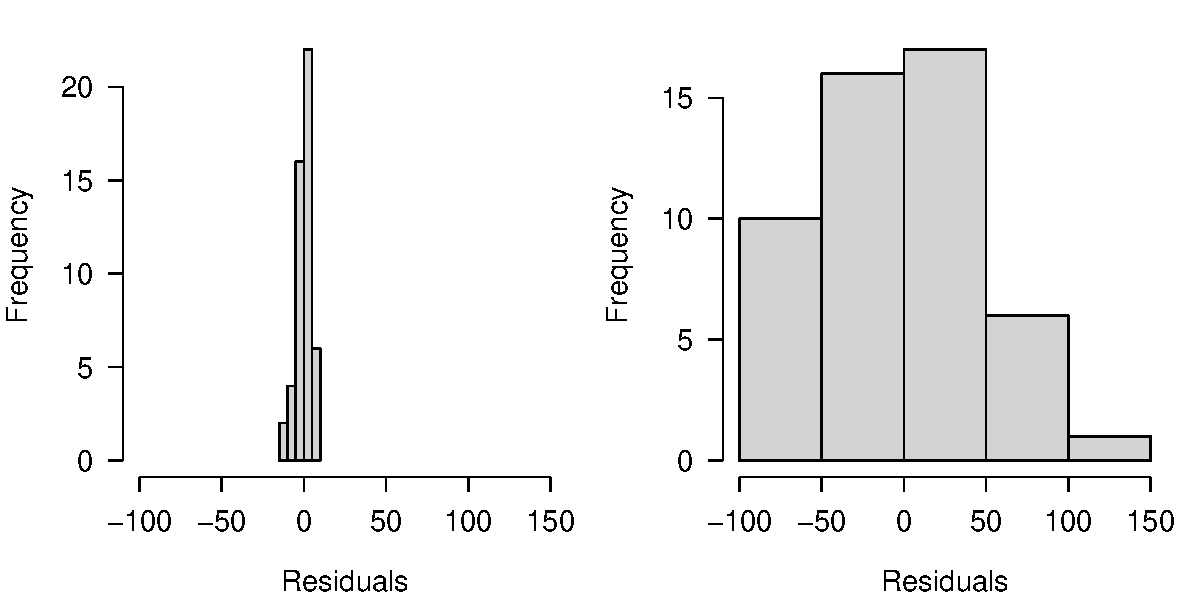
\includegraphics[keepaspectratio]{chapters/ch09_files/figure-pdf/unnamed-chunk-3-1.pdf}}
\end{center}

Notice also that both distributions of residuals have a similar shape,
despite the difference in width. This shape is actually very important:
the \textbf{normal distribution}. If the residuals were not distributed
this way (i.e., did not follow a normal distribution), then we would be
in trouble for two reasons. First, the data were generated using a
normal distribution for residuals, so something would have had to have
gone wrong with our statistical test; and second, the linear regression
model used to analyze the data assumes that residuals are normally
distributed. If they are not, then the test is not going to produce
valid estimates of statistical significance or model parameters.

The example above is an example of the importance of thinking about
statistical distributions when analyzing data. So just what is a
statistical distribution? Distributions are mathematical functions that
define the probabilities of random outcomes. Here \textbf{random} means
that there is some element of chance in what we observe. This randomness
is not completely unpredictable. While the outcome of specific
observations might be unknowable, we can make predictions about long run
frequencies or averages of lots of observations. In other words, single
observations are not predictable, but the properties of sets of
observations are. Such properties might include the number of times a
specific outcome occurs (e.g., number of times a flipped coin comes up
heads) or some summary of observations (e.g., the mean tail length of
chipmunks). Another term for this kind of randomness that follows a
pattern is \textbf{stochastic}.

\textbf{Another example: coin flips}

Consider flipping a coin. A fair coin will come up heads 50\% of the
time, and tails the other 50\%. If you flip a coin once, the probability
of getting heads is 50\%. But what about if you flip the coin 10 times?
How many heads should you get? 5 is a reasonable guess. The table below
shows the possible outcomes to 10 coin flips:

{\def\LTcaptype{none} % do not increment counter
\begin{longtable}[]{@{}cc@{}}
\toprule\noalign{}
Heads & Tails \\
\midrule\noalign{}
\endhead
\bottomrule\noalign{}
\endlastfoot
0 & 10 \\
1 & 9 \\
2 & 8 \\
3 & 7 \\
4 & 6 \\
5 & 5 \\
6 & 4 \\
7 & 3 \\
8 & 2 \\
9 & 1 \\
10 & 0 \\
\end{longtable}
}

This table shows that 5 heads is only one of 11 possibilities! So, is
the probability of 5 heads 1 in 11 (\(1/11\approx0.091\))? Of course
not, because not all outcomes are equally likely.

One of the reasons statistics is so fun is that we can often use
simulation to discover patterns. The R code below will simulate the
effects of flipping 1 coin 10 times. Run this code a few times and see
what happens.

\begin{Shaded}
\begin{Highlighting}[]
\FunctionTok{rbinom}\NormalTok{(}\DecValTok{1}\NormalTok{,}\DecValTok{10}\NormalTok{,}\FloatTok{0.5}\NormalTok{)}
\end{Highlighting}
\end{Shaded}

\begin{verbatim}
[1] 4
\end{verbatim}

A typical run of results might be something like
\texttt{4\ 5\ 5\ 4\ 3\ 5\ 6\ 6\ 5\ 5\ 4\ 6}. We can repeat this line
many times and graph the results:

\begin{Shaded}
\begin{Highlighting}[]
\NormalTok{x }\OtherTok{\textless{}{-}} \FunctionTok{numeric}\NormalTok{(}\DecValTok{20}\NormalTok{)}
\ControlFlowTok{for}\NormalTok{(i }\ControlFlowTok{in} \DecValTok{1}\SpecialCharTok{:}\DecValTok{20}\NormalTok{)\{x[i] }\OtherTok{\textless{}{-}} \FunctionTok{rbinom}\NormalTok{(}\DecValTok{1}\NormalTok{,}\DecValTok{10}\NormalTok{,}\FloatTok{0.5}\NormalTok{)\}}
\FunctionTok{plot}\NormalTok{(}\FunctionTok{table}\NormalTok{(x))}
\end{Highlighting}
\end{Shaded}

\begin{center}
\pandocbounded{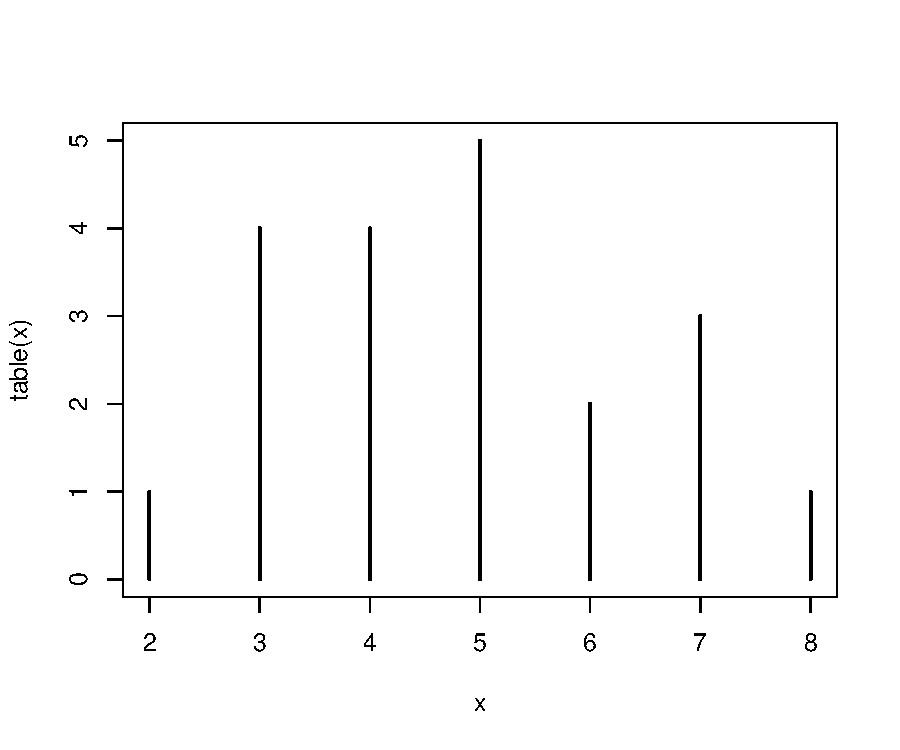
\includegraphics[keepaspectratio]{chapters/ch09_files/figure-pdf/unnamed-chunk-5-1.pdf}}
\end{center}

There is actually a faster way, by requesting 20 draws of 10 flips each
all at once:

\begin{Shaded}
\begin{Highlighting}[]
\NormalTok{x }\OtherTok{\textless{}{-}} \FunctionTok{rbinom}\NormalTok{(}\DecValTok{20}\NormalTok{,}\DecValTok{10}\NormalTok{,}\FloatTok{0.5}\NormalTok{)}
\FunctionTok{plot}\NormalTok{(}\FunctionTok{table}\NormalTok{(x))}
\end{Highlighting}
\end{Shaded}

\begin{center}
\pandocbounded{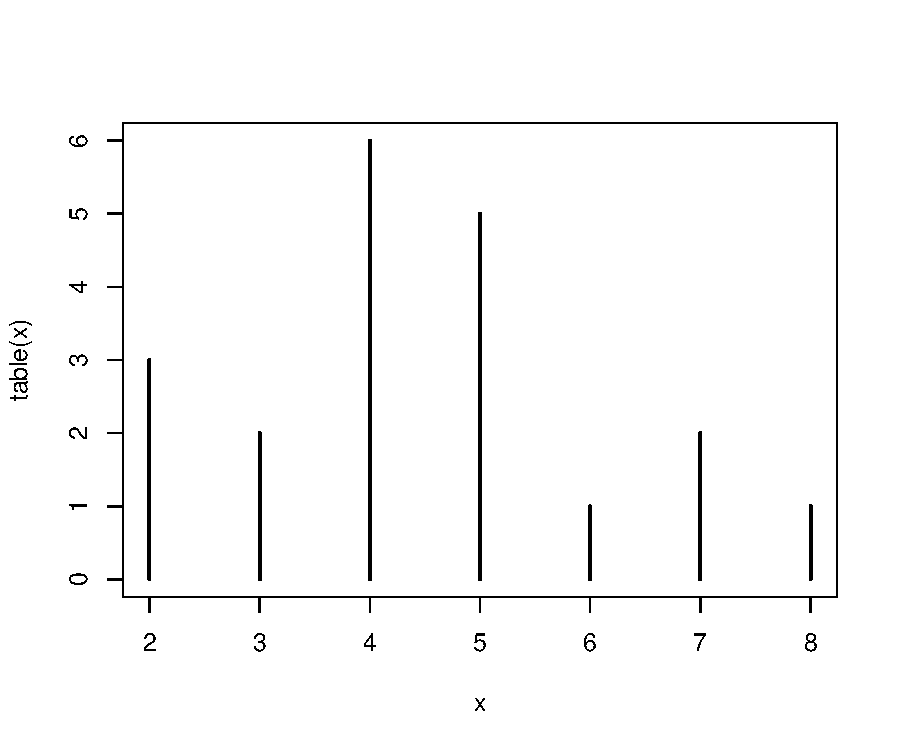
\includegraphics[keepaspectratio]{chapters/ch09_files/figure-pdf/unnamed-chunk-6-1.pdf}}
\end{center}

Is 5 the most likely value? What about if we get a larger sample?

\begin{Shaded}
\begin{Highlighting}[]
\NormalTok{x1 }\OtherTok{\textless{}{-}} \FunctionTok{table}\NormalTok{(}\FunctionTok{rbinom}\NormalTok{(}\DecValTok{10}\NormalTok{,}\DecValTok{10}\NormalTok{,}\FloatTok{0.5}\NormalTok{))}
\NormalTok{x2 }\OtherTok{\textless{}{-}} \FunctionTok{table}\NormalTok{(}\FunctionTok{rbinom}\NormalTok{(}\DecValTok{100}\NormalTok{,}\DecValTok{10}\NormalTok{,}\FloatTok{0.5}\NormalTok{))}
\NormalTok{x3 }\OtherTok{\textless{}{-}} \FunctionTok{table}\NormalTok{(}\FunctionTok{rbinom}\NormalTok{(}\DecValTok{1000}\NormalTok{,}\DecValTok{10}\NormalTok{,}\FloatTok{0.5}\NormalTok{))}
\NormalTok{x4 }\OtherTok{\textless{}{-}} \FunctionTok{table}\NormalTok{(}\FunctionTok{rbinom}\NormalTok{(}\DecValTok{10000}\NormalTok{,}\DecValTok{10}\NormalTok{,}\FloatTok{0.5}\NormalTok{))}
\NormalTok{x5 }\OtherTok{\textless{}{-}} \FunctionTok{table}\NormalTok{(}\FunctionTok{rbinom}\NormalTok{(}\DecValTok{100000}\NormalTok{,}\DecValTok{10}\NormalTok{,}\FloatTok{0.5}\NormalTok{))}
\NormalTok{x6 }\OtherTok{\textless{}{-}} \FunctionTok{table}\NormalTok{(}\FunctionTok{rbinom}\NormalTok{(}\DecValTok{1000000}\NormalTok{,}\DecValTok{10}\NormalTok{,}\FloatTok{0.5}\NormalTok{))}

\FunctionTok{par}\NormalTok{(}\AttributeTok{mfrow=}\FunctionTok{c}\NormalTok{(}\DecValTok{2}\NormalTok{,}\DecValTok{3}\NormalTok{))}
\FunctionTok{plot}\NormalTok{(x1, }\AttributeTok{xlim=}\FunctionTok{c}\NormalTok{(}\DecValTok{0}\NormalTok{, }\DecValTok{10}\NormalTok{), }\AttributeTok{main=}\StringTok{"n = 10"}\NormalTok{)}
\FunctionTok{plot}\NormalTok{(x2, }\AttributeTok{xlim=}\FunctionTok{c}\NormalTok{(}\DecValTok{0}\NormalTok{, }\DecValTok{10}\NormalTok{), }\AttributeTok{main=}\StringTok{"n = 100"}\NormalTok{)}
\FunctionTok{plot}\NormalTok{(x3, }\AttributeTok{xlim=}\FunctionTok{c}\NormalTok{(}\DecValTok{0}\NormalTok{, }\DecValTok{10}\NormalTok{), }\AttributeTok{main=}\StringTok{"n = 1000"}\NormalTok{)}
\FunctionTok{plot}\NormalTok{(x4, }\AttributeTok{xlim=}\FunctionTok{c}\NormalTok{(}\DecValTok{0}\NormalTok{, }\DecValTok{10}\NormalTok{), }\AttributeTok{main=}\StringTok{"n = 10000"}\NormalTok{)}
\FunctionTok{plot}\NormalTok{(x5, }\AttributeTok{xlim=}\FunctionTok{c}\NormalTok{(}\DecValTok{0}\NormalTok{, }\DecValTok{10}\NormalTok{), }\AttributeTok{main=}\StringTok{"n = 100000"}\NormalTok{)}
\FunctionTok{plot}\NormalTok{(x6, }\AttributeTok{xlim=}\FunctionTok{c}\NormalTok{(}\DecValTok{0}\NormalTok{, }\DecValTok{10}\NormalTok{), }\AttributeTok{main=}\StringTok{"n = 1000000"}\NormalTok{)}
\end{Highlighting}
\end{Shaded}

\begin{center}
\pandocbounded{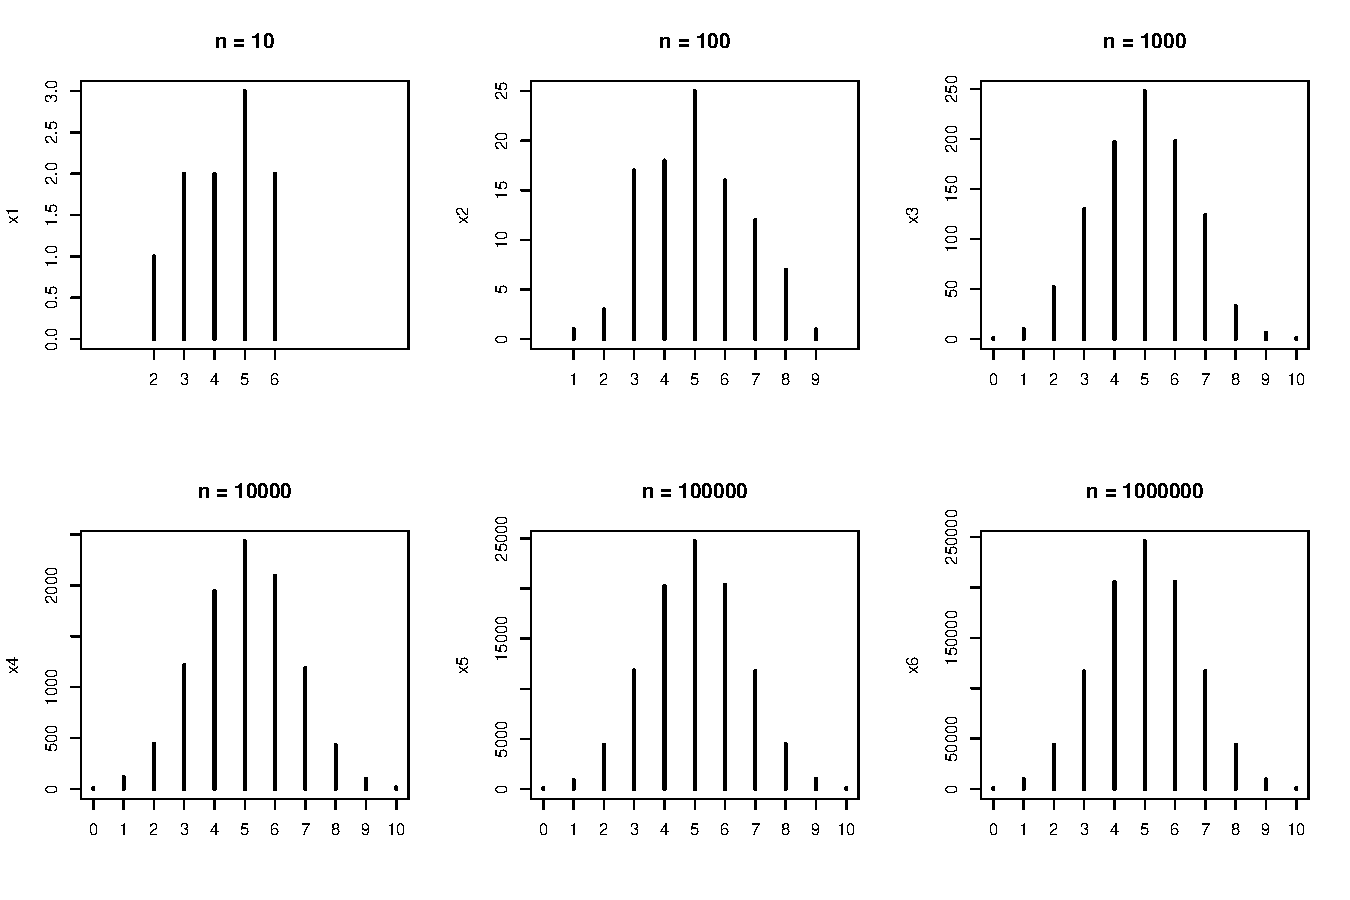
\includegraphics[keepaspectratio]{chapters/ch09_files/figure-pdf/unnamed-chunk-7-1.pdf}}
\end{center}

\begin{Shaded}
\begin{Highlighting}[]
\CommentTok{\# reset graphical parameters}
\FunctionTok{par}\NormalTok{(}\AttributeTok{mfrow=}\FunctionTok{c}\NormalTok{(}\DecValTok{1}\NormalTok{,}\DecValTok{1}\NormalTok{))}
\end{Highlighting}
\end{Shaded}

You may have guessed by now that the properties of a set of coin
flips---such as what number of heads to expect---are described by some
kind of mathematical function. This function is called a
\textbf{probability distribution}. This particular distribution is the
\textbf{binomial distribution}, which describes the outcome of any
random process with a binary outcome. The name ``binomial'' is
descriptive: ``bi'' for two, and ``nomial'' for names or states. Can you
think of a biological situation where the binomial distribution might
apply?

The sections below describe some distributions commonly encountered in
biology, and what kinds of processes give rise to them. It is important
to be able to relate biological phenomena to statistical distributions,
because the underlying nature of the randomness in some process can
affect how we analyze that process statistically. Note that in this
class we will focus on the practical applications of these
distributions, rather than their mathematical derivations.

\subsection{Probability distributions in R}\label{sec-dist-r}

Every distribution supported in R has four functions associated with it:
\texttt{r\_\_()}, \texttt{q\_\_()}, \texttt{d\_\_()}, and
\texttt{p\_\_()} , where \texttt{\_\_} is the name of the distribution
(or an abbreviation). These 4 functions calculate different values
defined by the distribution:

\begin{itemize}
\tightlist
\item
  \texttt{r\_\_()} draws \textbf{random numbers} from the distribution.
\item
  \texttt{p\_\_()} calculates the \textbf{cumulative distribution
  function (CDF)} at a given value. The reverse of \texttt{q\_\_()}.
\item
  \texttt{d\_\_()} calculates the \textbf{probability density function
  (PDF)}; i.e., the height of the density curve, or first derivative of
  the CDF.
\item
  \texttt{q\_\_()} calculates the \textbf{value at a given quantile}.
  The reverse of \texttt{p\_\_()}.
\end{itemize}

The figure below shows these functions in relation to the PDF and CDF
for a normal distribution.

\begin{center}
\pandocbounded{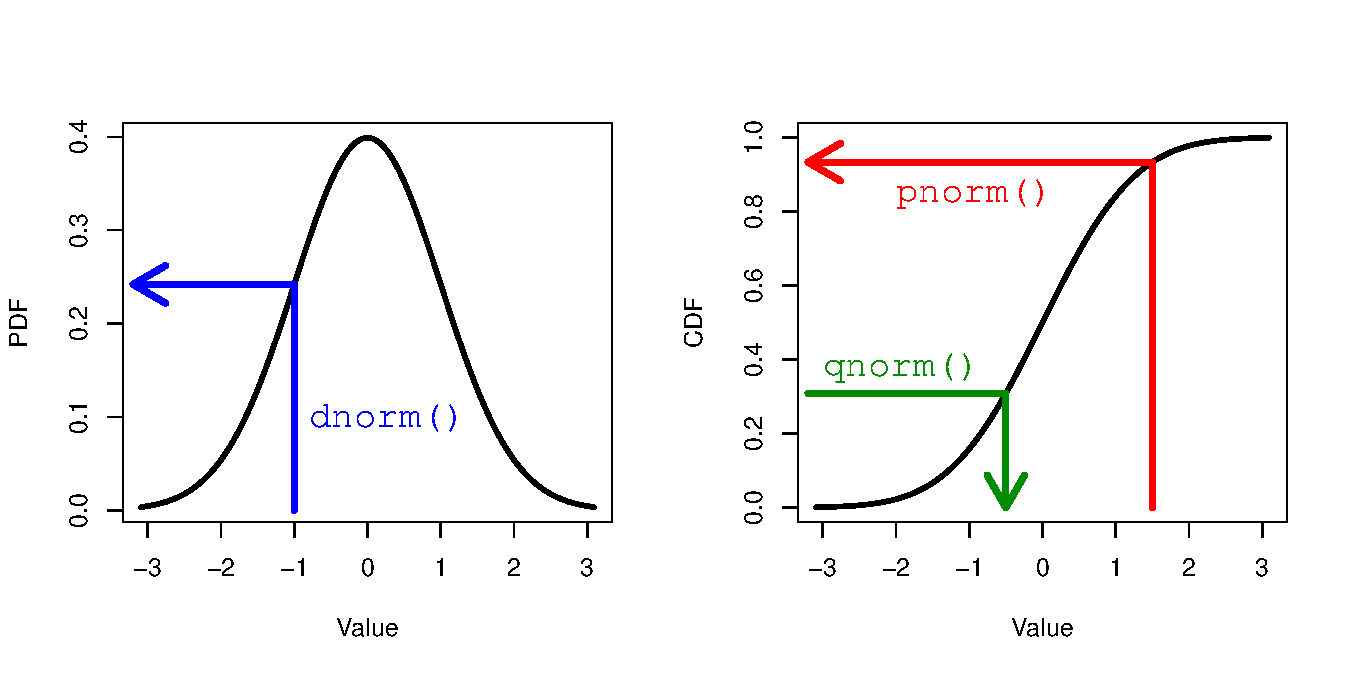
\includegraphics[keepaspectratio]{chapters/ch09_files/figure-pdf/unnamed-chunk-8-1.pdf}}
\end{center}

\begin{itemize}
\tightlist
\item
  If you want to know the value at the Xth percentile of a distribution,
  use the \texttt{q\_\_} function.
\item
  If you want to know the percentile of a value of a distribution, use
  the \texttt{p\_\_} function.
\item
  If you need to know the PDF of a distribution at some value, use the
  \texttt{d\_\_} function.
\end{itemize}

Here we see the functions used on a normal distribution with mean 20 and
SD 4 (i.e., \(Normal\left(\mu=20,\sigma=4\right)\) or
\(N\left(20,4\right)\)).

\begin{Shaded}
\begin{Highlighting}[]
\CommentTok{\# 0.3 quantile (30th percentile)}
\FunctionTok{qnorm}\NormalTok{(}\FloatTok{0.3}\NormalTok{, }\DecValTok{20}\NormalTok{, }\DecValTok{4}\NormalTok{)}
\end{Highlighting}
\end{Shaded}

\begin{verbatim}
[1] 17.9024
\end{verbatim}

\begin{Shaded}
\begin{Highlighting}[]
\CommentTok{\# What value is at the 64th percentile? (0.64 quantile)?}
\FunctionTok{pnorm}\NormalTok{(}\FloatTok{0.65}\NormalTok{, }\DecValTok{20}\NormalTok{,}\DecValTok{4}\NormalTok{)}
\end{Highlighting}
\end{Shaded}

\begin{verbatim}
[1] 6.574119e-07
\end{verbatim}

\begin{Shaded}
\begin{Highlighting}[]
\CommentTok{\# What is the PDF at x == 23?}
\FunctionTok{dnorm}\NormalTok{(}\DecValTok{23}\NormalTok{, }\DecValTok{20}\NormalTok{, }\DecValTok{4}\NormalTok{)}
\end{Highlighting}
\end{Shaded}

\begin{verbatim}
[1] 0.07528436
\end{verbatim}

One use case might be drawing a CDF or PDF of a distribution manually to
compare to your data or some other distribution. For example, here is
how to draw the CDF of a normal with mean 10 and SD 2:

\begin{Shaded}
\begin{Highlighting}[]
\CommentTok{\# values at which to draw CDF}
\NormalTok{xvals }\OtherTok{\textless{}{-}} \FunctionTok{seq}\NormalTok{(}\DecValTok{0}\NormalTok{, }\DecValTok{20}\NormalTok{, }\AttributeTok{length=}\DecValTok{1000}\NormalTok{)}

\CommentTok{\# distribution parameters}
\NormalTok{mu }\OtherTok{\textless{}{-}} \DecValTok{10}
\NormalTok{sigma }\OtherTok{\textless{}{-}} \DecValTok{2}

\CommentTok{\# calculate CDF}
\NormalTok{xcdf }\OtherTok{\textless{}{-}} \FunctionTok{pnorm}\NormalTok{(xvals, mu, sigma)}

\CommentTok{\# make the plot}
\FunctionTok{plot}\NormalTok{(xvals, xcdf, }\AttributeTok{type=}\StringTok{"l"}\NormalTok{, }\AttributeTok{xlab=}\StringTok{"Value of x"}\NormalTok{, }\AttributeTok{ylab=}\StringTok{"CDF(x)"}\NormalTok{)}
\end{Highlighting}
\end{Shaded}

\pandocbounded{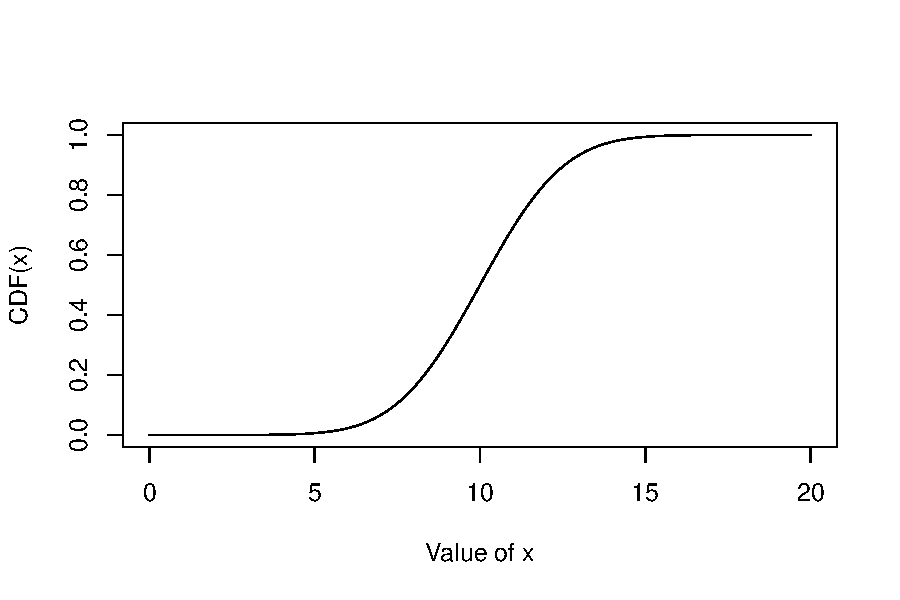
\includegraphics[keepaspectratio]{chapters/ch09_files/figure-pdf/unnamed-chunk-12-1.pdf}}

Here is how to draw the PDF of the same distribution:

\begin{Shaded}
\begin{Highlighting}[]
\CommentTok{\# calculate CDF}
\NormalTok{xpdf }\OtherTok{\textless{}{-}} \FunctionTok{dnorm}\NormalTok{(xvals, mu, sigma)}

\CommentTok{\# make the plot}
\FunctionTok{plot}\NormalTok{(xvals, xpdf, }\AttributeTok{type=}\StringTok{"l"}\NormalTok{, }\AttributeTok{xlab=}\StringTok{"Value of x"}\NormalTok{,}
     \AttributeTok{ylab=}\StringTok{"Probability density of x"}\NormalTok{)}
\end{Highlighting}
\end{Shaded}

\pandocbounded{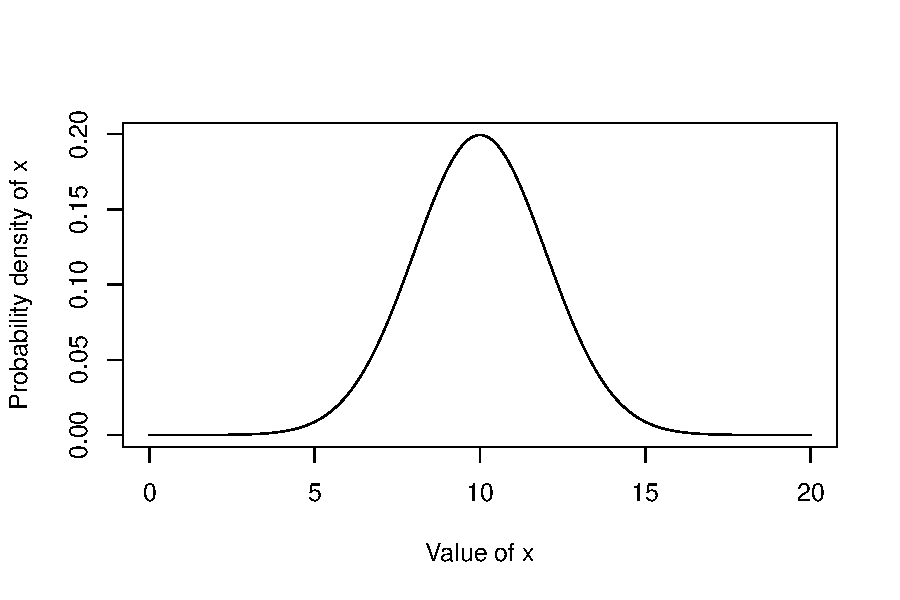
\includegraphics[keepaspectratio]{chapters/ch09_files/figure-pdf/unnamed-chunk-13-1.pdf}}

\section{Discrete distributions}\label{sec-dist-disc}

\textbf{Discrete distributions} can take on integer values only. Because
of this, many discrete distributions are related in some way to
\textbf{count data}. Count data result from, well, counting things.
Count data can also describe the number of times something happened.

\subsection{Bernoulli distribution}\label{sec-dist-bern}

The simplest discrete distribution is the \textbf{Bernoulli
distribution}. It describes the outcome of a single random event with
probability \emph{p}. Thus, the Bernoulli distribution takes the value 1
with probability \emph{p} or the value 0 with probability
\(q=\left(1-p\right)\). Any opportunity for the event to happen is also
called a \textbf{Bernoulli trial}, and the process that it describes a
\textbf{Bernoulli process}. The probability \emph{p} can take on any
value in the closed interval \(\left[0,1\right]\).

For convenience we usually consider a Bernoulli distribution to take the
value of 0 or 1, but really it could represent any binary outcome. For
example, \emph{yes vs.~no}, \emph{dead vs.~alive}, \(<3\) vs.~\(\ge3\),
etc., are all outcomes that could be modeled as Bernoulli variables. By
convention, the event that occurs with probability \emph{p} is
considered a \textbf{success} and has the numerical value 1; the event
that occurs with probability \(1-p\) is considered a \textbf{failure}
and takes the numerical value 0. This is how Bernoulli variables are
represented in most statistical packages, including R.

The Bernoulli distribution is rarely used on its own in an analysis.
Instead, it's useful to think of the Bernoulli distribution as a special
case of, or a building block of, more complicated distributions such as
the \textbf{binomial distribution} (Section~\ref{sec-dist-binom}). For
example, a single observation of a binomially-distributed variable could
be thought of as a Bernoulli distribution.

The Bernoulli distribution is a special case of the binomial
distribution, and so it is accessed in R using the functions associated
with the binomial. With the \texttt{size} argument set to 1, the
binomial distribution \emph{is} the Bernoulli distribution.

\begin{Shaded}
\begin{Highlighting}[]
\CommentTok{\# flip one fair coin}
\FunctionTok{rbinom}\NormalTok{(}\DecValTok{1}\NormalTok{, }\DecValTok{1}\NormalTok{, }\FloatTok{0.5}\NormalTok{)}
\end{Highlighting}
\end{Shaded}

\begin{verbatim}
[1] 0
\end{verbatim}

\begin{Shaded}
\begin{Highlighting}[]
\CommentTok{\# flip 10 fair coins}
\FunctionTok{rbinom}\NormalTok{(}\DecValTok{10}\NormalTok{, }\DecValTok{1}\NormalTok{, }\FloatTok{0.5}\NormalTok{)}
\end{Highlighting}
\end{Shaded}

\begin{verbatim}
 [1] 1 1 0 1 1 0 1 0 1 1
\end{verbatim}

\begin{Shaded}
\begin{Highlighting}[]
\CommentTok{\# flip 10 coins with a 70\% chance of heads}
\FunctionTok{rbinom}\NormalTok{(}\DecValTok{10}\NormalTok{, }\DecValTok{1}\NormalTok{, }\FloatTok{0.7}\NormalTok{)}
\end{Highlighting}
\end{Shaded}

\begin{verbatim}
 [1] 0 1 1 0 1 1 0 0 0 1
\end{verbatim}

\subsection{Binomial distribution}\label{sec-dist-binom}

The binomial distribution describes the \textbf{number of successes} in
a set of independent Bernoulli trials. Each trial has probability of
success \emph{p}, and there are \emph{n} trials. The values \emph{n} and
\emph{p} are the \textbf{parameters} of the binomial distribution--the
values that describe its behavior. The coin flipping example above is an
example of a binomial distribution. Biological examples of binomial
processes might be the number of fish that die in an experiment, or the
number of plants that flower in a season. In such a case, the number of
fish that start the experiment is the sample size \emph{n} and the
individual mortality rate is \emph{p}.

Because it is so simple, thinking about the binomial distribution is a
good warm up for learning about the characteristics of probability
distributions. One of the most important characteristics is the
\textbf{expected value} of the distribution. This is the value that most
likely to occur, or the \textbf{central tendency} of values. There are
several kinds of expected value, but they are all related to the most
common or central value. The expected value, or mean, of a binomial
distribution \emph{X} is

\[E\left(x\right)=\mu=np\]

This is the answer to the question earlier about how many heads to
expect if a fair coin is flipped 10 times:

\[E(heads)=n(flips)p(heads)\]

If a variable comes from a binomial process, we can make other
inferences about it. For example, we can estimate its variance as:

\[Var\left(x\right)=\sigma^2=np(1-p)=npq\]

We can also estimate the probability of any number of successes \emph{k}
as:

\[P\left(k\right)=\left(\begin{matrix}n\\k\\\end{matrix}\right)p^k\left(1-p\right)^{n-k}\]

The first term (\emph{n} over \emph{k}) is known as the \textbf{binomial
coefficient} and is calculated as:

\[\left(\begin{matrix}n\\k\\\end{matrix}\right)=\frac{n!}{k!\left(n-k\right)!}\]

This term represents the number of ways of seeing \emph{k} successes in
\emph{n} trials. For example, a set of 4 trials could have 2 successes
in 6 ways: HHTT, HTHT, THHT, HTTH, THTH, and TTHH.

When \emph{n} is small, the binomial distribution can be quite skewed
(i.e., asymmetric) because the distribution has a hard lower bound of 0.
Note that the expression for \(P(k)\) is what is calculated by function
\texttt{dbinom()} below, and related to what is calculated by function
\texttt{pbinom()}. For large \emph{n}, the binomial distribution can be
approximated by a normal distribution\footnote{Although the values must
  be rounded to non-negative integers!} with mean = \emph{np} and
variance = \emph{npq}.

\subsubsection{Binomial distribution in R}\label{sec-dist-binom-r}

R uses a family of 4 functions to work with each probability
distribution. The binomial and Bernoulli distributions are accessed
using the \texttt{\_binom} group of functions: \texttt{dbinom()},
\texttt{pbinom()}, \texttt{qbinom()}, and \texttt{rbinom()}. Each
function calculates or returns something different about the binomial
distribution:

\begin{itemize}
\tightlist
\item
  \texttt{dbinom()}: Calculates probability mass function at \emph{x}
  for binomial distribution given \emph{n} and \emph{p}. Answers the
  question ``What is the probability of \emph{x} successes in \emph{n}
  trials with probability \emph{p}?''
\item
  \texttt{pbinom()}: Calculates integral of the probability mass
  function for a binomial distribution given \emph{n} and \emph{p}, from
  0 up to \emph{x}. In other words, given some binomial distribution, at
  what quantile of that distribution should some value fall? The reverse
  of \texttt{qbinom()}. Answers the question ``What is the probably of
  at least \emph{x} successes in \emph{n} trials with probability
  \emph{p}?''
\item
  \texttt{qbinom()}: Calculates the value at specified quantile of a
  binomial distribution. Essentially the reverse of \texttt{pbinom()}.
\item
  \texttt{rbinom()}: Draws random numbers from the binomial distribution
  defined by \emph{n} and \emph{p} (or from the Bernoulli distribution
  if \emph{n} = 1).
\end{itemize}

Let's explore the binomial distribution using these functions. In the
plots produced in the two examples, notice how the variance of each
distribution (\texttt{x1}, \texttt{x2}, etc.) depends on both n and
p.~The variance in these plots is shown by the width of the
distribution.

\begin{Shaded}
\begin{Highlighting}[]
\CommentTok{\# N = 100, P various}
\NormalTok{N }\OtherTok{\textless{}{-}} \DecValTok{100}
\NormalTok{X }\OtherTok{\textless{}{-}} \DecValTok{0}\SpecialCharTok{:}\DecValTok{100}
\NormalTok{x1 }\OtherTok{\textless{}{-}} \FunctionTok{dbinom}\NormalTok{(X, N, }\FloatTok{0.2}\NormalTok{)}
\NormalTok{x2 }\OtherTok{\textless{}{-}} \FunctionTok{dbinom}\NormalTok{(X, N, }\FloatTok{0.4}\NormalTok{)}
\NormalTok{x3 }\OtherTok{\textless{}{-}} \FunctionTok{dbinom}\NormalTok{(X, N, }\FloatTok{0.6}\NormalTok{)}
\NormalTok{x4 }\OtherTok{\textless{}{-}} \FunctionTok{dbinom}\NormalTok{(X, N, }\FloatTok{0.8}\NormalTok{)}

\FunctionTok{par}\NormalTok{(}\AttributeTok{mfrow=}\FunctionTok{c}\NormalTok{(}\DecValTok{1}\NormalTok{,}\DecValTok{1}\NormalTok{))}
\FunctionTok{plot}\NormalTok{(X, x1, }\AttributeTok{pch=}\DecValTok{16}\NormalTok{, }\AttributeTok{xlab=}\StringTok{"X"}\NormalTok{, }\AttributeTok{ylab=}\StringTok{"PMF"}\NormalTok{)}
\FunctionTok{points}\NormalTok{(X, x2, }\AttributeTok{pch=}\DecValTok{16}\NormalTok{, }\AttributeTok{col=}\StringTok{"red"}\NormalTok{)}
\FunctionTok{points}\NormalTok{(X, x3, }\AttributeTok{pch=}\DecValTok{16}\NormalTok{, }\AttributeTok{col=}\StringTok{"blue"}\NormalTok{)}
\FunctionTok{points}\NormalTok{(X, x4, }\AttributeTok{pch=}\DecValTok{16}\NormalTok{, }\AttributeTok{col=}\StringTok{"green"}\NormalTok{)}
\end{Highlighting}
\end{Shaded}

\begin{center}
\pandocbounded{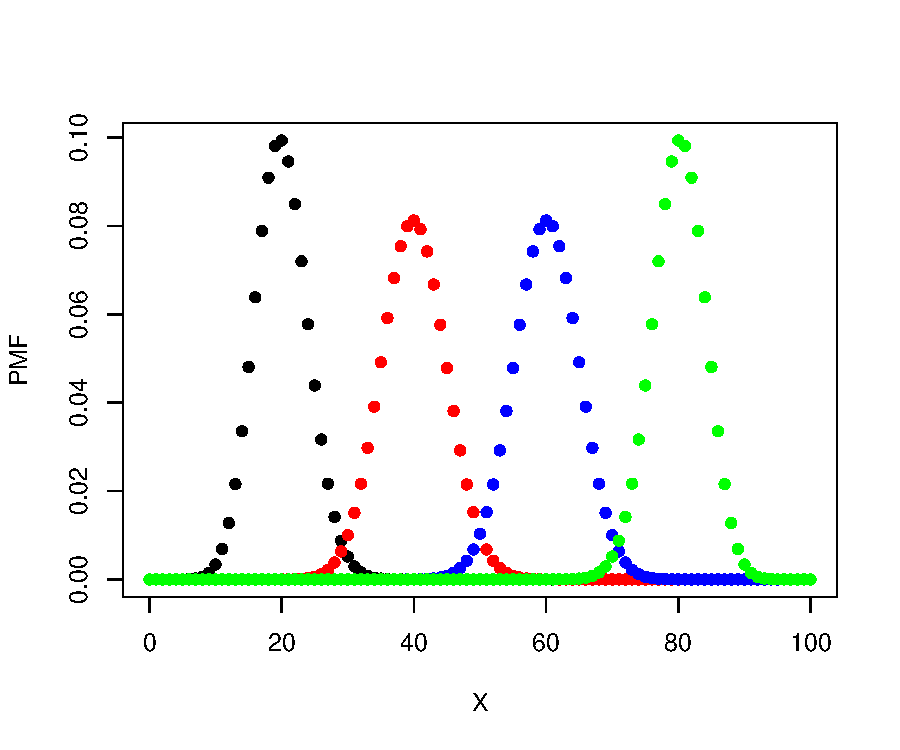
\includegraphics[keepaspectratio]{chapters/ch09_files/figure-pdf/unnamed-chunk-15-1.pdf}}
\end{center}

Here is a plot showing the effect of varying \emph{n}.

\begin{Shaded}
\begin{Highlighting}[]
\CommentTok{\# P = 0.5, N various}
\NormalTok{P }\OtherTok{\textless{}{-}} \FloatTok{0.5}
\NormalTok{x1 }\OtherTok{\textless{}{-}} \FunctionTok{dbinom}\NormalTok{(}\DecValTok{0}\SpecialCharTok{:}\DecValTok{100}\NormalTok{, }\DecValTok{20}\NormalTok{, P)}
\NormalTok{x2 }\OtherTok{\textless{}{-}} \FunctionTok{dbinom}\NormalTok{(}\DecValTok{0}\SpecialCharTok{:}\DecValTok{100}\NormalTok{, }\DecValTok{40}\NormalTok{, P)}
\NormalTok{x3 }\OtherTok{\textless{}{-}} \FunctionTok{dbinom}\NormalTok{(}\DecValTok{0}\SpecialCharTok{:}\DecValTok{100}\NormalTok{, }\DecValTok{60}\NormalTok{, P)}
\NormalTok{x4 }\OtherTok{\textless{}{-}} \FunctionTok{dbinom}\NormalTok{(}\DecValTok{0}\SpecialCharTok{:}\DecValTok{100}\NormalTok{, }\DecValTok{80}\NormalTok{, P)}
\NormalTok{x5 }\OtherTok{\textless{}{-}} \FunctionTok{dbinom}\NormalTok{(}\DecValTok{0}\SpecialCharTok{:}\DecValTok{100}\NormalTok{, }\DecValTok{100}\NormalTok{, P)}

\FunctionTok{plot}\NormalTok{(}\DecValTok{0}\SpecialCharTok{:}\DecValTok{100}\NormalTok{, x1, }\AttributeTok{pch=}\DecValTok{16}\NormalTok{, }\AttributeTok{xlab=}\StringTok{"X"}\NormalTok{, }\AttributeTok{ylab=}\StringTok{"PMF"}\NormalTok{)}
\FunctionTok{points}\NormalTok{(}\DecValTok{0}\SpecialCharTok{:}\DecValTok{100}\NormalTok{, x2, }\AttributeTok{pch=}\DecValTok{16}\NormalTok{, }\AttributeTok{col=}\StringTok{"red"}\NormalTok{)}
\FunctionTok{points}\NormalTok{(}\DecValTok{0}\SpecialCharTok{:}\DecValTok{100}\NormalTok{, x3, }\AttributeTok{pch=}\DecValTok{16}\NormalTok{, }\AttributeTok{col=}\StringTok{"blue"}\NormalTok{)}
\FunctionTok{points}\NormalTok{(}\DecValTok{0}\SpecialCharTok{:}\DecValTok{100}\NormalTok{, x4, }\AttributeTok{pch=}\DecValTok{16}\NormalTok{, }\AttributeTok{col=}\StringTok{"green"}\NormalTok{)}
\FunctionTok{points}\NormalTok{(}\DecValTok{0}\SpecialCharTok{:}\DecValTok{100}\NormalTok{, x5, }\AttributeTok{pch=}\DecValTok{16}\NormalTok{, }\AttributeTok{col=}\StringTok{"purple"}\NormalTok{)}
\end{Highlighting}
\end{Shaded}

\begin{center}
\pandocbounded{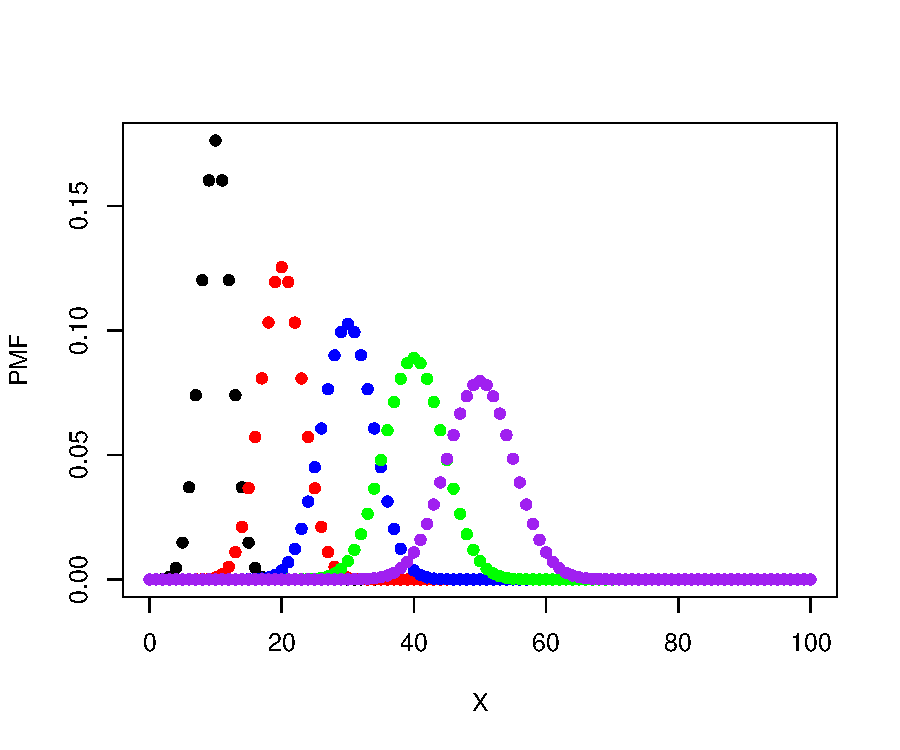
\includegraphics[keepaspectratio]{chapters/ch09_files/figure-pdf/chunkx400-1.pdf}}
\end{center}

In these plots, the height of the points is called the
\textbf{probability mass function (PMF)}. For discrete distributions
like the binomial, the PMF of any value is the probability that the
distribution takes on that value. The sum of the PMF for all integers
from 0 to \emph{n} (inclusive) must be equal to 1. You can verify this
by calculating the sum of any of the vectors of densities above.

The function \texttt{pbinom()} sums the PMF from 0 up to and including
some value. In other words, it calculates the \textbf{cumulative
distribution function (CDF)}. This answers the question ``where in the
distribution is value \emph{x}?''; put another way, ``at what quantile
of the distribution does value \emph{x} lie?''. Yet another way to ask
this is, ``What is the probability of at least \emph{X} successes?''.

Consider a binomial distribution with \(n=10\) and \(p=0.5\). What is
the probability that the distribution takes a value \(\le7\)? We can
calculate this as the sum of the PMF for 0 through 7.

\begin{Shaded}
\begin{Highlighting}[]
\CommentTok{\# plot the distribution to see it}
\NormalTok{N }\OtherTok{\textless{}{-}} \DecValTok{10}
\NormalTok{P }\OtherTok{\textless{}{-}} \FloatTok{0.5}
\NormalTok{xd }\OtherTok{\textless{}{-}} \FunctionTok{dbinom}\NormalTok{(}\DecValTok{0}\SpecialCharTok{:}\DecValTok{10}\NormalTok{, N, P)}
\FunctionTok{plot}\NormalTok{(}\DecValTok{0}\SpecialCharTok{:}\DecValTok{10}\NormalTok{, xd, }\AttributeTok{type=}\StringTok{"h"}\NormalTok{, }\AttributeTok{xlab=}\StringTok{"X"}\NormalTok{, }\AttributeTok{ylab=}\StringTok{"PMF"}\NormalTok{)}
\end{Highlighting}
\end{Shaded}

\begin{center}
\pandocbounded{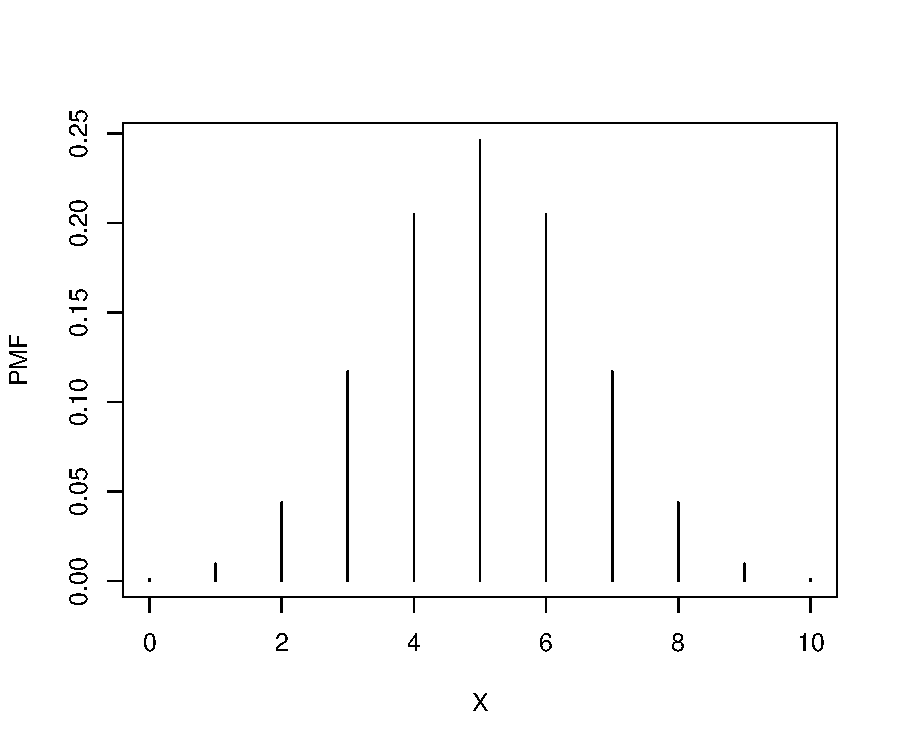
\includegraphics[keepaspectratio]{chapters/ch09_files/figure-pdf/unnamed-chunk-16-1.pdf}}
\end{center}

\begin{Shaded}
\begin{Highlighting}[]
\CommentTok{\# calculate p(x\textless{}=7)}
\FunctionTok{sum}\NormalTok{(xd[}\DecValTok{1}\SpecialCharTok{:}\DecValTok{8}\NormalTok{]) }\CommentTok{\# indices 1:8 correspond to values 0:7}
\end{Highlighting}
\end{Shaded}

\begin{verbatim}
[1] 0.9453125
\end{verbatim}

\begin{Shaded}
\begin{Highlighting}[]
\CommentTok{\# same value:}
\FunctionTok{pbinom}\NormalTok{(}\DecValTok{7}\NormalTok{, N, P)}
\end{Highlighting}
\end{Shaded}

\begin{verbatim}
[1] 0.9453125
\end{verbatim}

Or, we could want to know the probability that the distribution takes on
a value \(>6\). This would be the complement of the sum up to and
including 6.

\begin{Shaded}
\begin{Highlighting}[]
\DecValTok{1}\SpecialCharTok{{-}}\FunctionTok{sum}\NormalTok{(xd[}\DecValTok{1}\SpecialCharTok{:}\DecValTok{7}\NormalTok{])}
\end{Highlighting}
\end{Shaded}

\begin{verbatim}
[1] 0.171875
\end{verbatim}

\begin{Shaded}
\begin{Highlighting}[]
\CommentTok{\# same value:}
\DecValTok{1}\SpecialCharTok{{-}}\FunctionTok{pbinom}\NormalTok{(}\DecValTok{6}\NormalTok{,N,P)}
\end{Highlighting}
\end{Shaded}

\begin{verbatim}
[1] 0.171875
\end{verbatim}

If the last two calculations seem familiar, that's because this is
exactly how \emph{p}-values for statistical tests are calculated (e.g.,
using \texttt{pf()} to get the probability from an \emph{F} distribution
for an ANOVA).

The function \texttt{qbinom()} is basically the reverse of function
\texttt{pbinom()}. Rather than calculate the quantile at which a value
falls in the distribution, \texttt{qbinom()} calculates the value at
which a quantile falls. For example, what value do we expect to find at
the 60th percentile of a distribution? Put another way, how many
successes should 60\% of experiments have, on average? The example below
shows how \texttt{qbinom()} and \texttt{pbinom()} are reversible.

\begin{Shaded}
\begin{Highlighting}[]
\NormalTok{N }\OtherTok{\textless{}{-}} \DecValTok{10}
\NormalTok{P }\OtherTok{\textless{}{-}} \FloatTok{0.5}
\FunctionTok{pbinom}\NormalTok{(}\DecValTok{6}\NormalTok{, N, P)}
\end{Highlighting}
\end{Shaded}

\begin{verbatim}
[1] 0.828125
\end{verbatim}

\begin{Shaded}
\begin{Highlighting}[]
\CommentTok{\# same value}
\FunctionTok{qbinom}\NormalTok{(}\FloatTok{0.828125}\NormalTok{, N, P)}
\end{Highlighting}
\end{Shaded}

\begin{verbatim}
[1] 6
\end{verbatim}

Finally, \texttt{rbinom()} draws random values from the binomial or
Bernoulli distributions. The syntax of this function can be a little
confusing. The first argument, \texttt{n}, is the \emph{number of random
draws} that you want. The second argument, \texttt{size}, is the
\emph{number of values in each draw}; that is, the parameter \emph{n} of
the binomial distribution. Compare these results, all with \emph{p} =
0.5:

\begin{Shaded}
\begin{Highlighting}[]
\CommentTok{\# 1 draw of 1 trial}
\FunctionTok{rbinom}\NormalTok{(}\DecValTok{1}\NormalTok{, }\DecValTok{1}\NormalTok{, }\FloatTok{0.5}\NormalTok{)}
\end{Highlighting}
\end{Shaded}

\begin{verbatim}
[1] 0
\end{verbatim}

\begin{Shaded}
\begin{Highlighting}[]
\CommentTok{\# 1 draw of 10 trials}
\FunctionTok{rbinom}\NormalTok{(}\DecValTok{1}\NormalTok{, }\DecValTok{10}\NormalTok{, }\FloatTok{0.5}\NormalTok{)}
\end{Highlighting}
\end{Shaded}

\begin{verbatim}
[1] 8
\end{verbatim}

\begin{Shaded}
\begin{Highlighting}[]
\CommentTok{\# 10 draws of 1 trial per draw }
\FunctionTok{rbinom}\NormalTok{(}\DecValTok{10}\NormalTok{, }\DecValTok{1}\NormalTok{, }\FloatTok{0.5}\NormalTok{)}
\end{Highlighting}
\end{Shaded}

\begin{verbatim}
 [1] 0 0 1 0 1 1 1 0 1 0
\end{verbatim}

\begin{Shaded}
\begin{Highlighting}[]
\CommentTok{\# 10 draws of 10 trials per draw}
\FunctionTok{rbinom}\NormalTok{(}\DecValTok{10}\NormalTok{, }\DecValTok{10}\NormalTok{, }\FloatTok{0.5}\NormalTok{)}
\end{Highlighting}
\end{Shaded}

\begin{verbatim}
 [1] 3 5 5 7 3 5 5 5 4 3
\end{verbatim}

\begin{itemize}
\tightlist
\item
  Result 1 shows a Bernoulli distribution with \emph{n} = 1.
\item
  Result 2 shows a single value from a binomial distribution with
  \emph{n} = 10.
\item
  Result 3 shows 10 results from Bernoulli distributions. Notice that if
  you add up the values in Result 3, you get a result like Result 2.
\item
  Finally, Result 4 shows 10 draws from a binomial distribution, which
  itself has \emph{n} = 10.
\end{itemize}

The take home message is that the first argument to \texttt{rbinom()} is
not a parameter of the binomial distribution. It is instead the number
of draws from the distribution that you want. The \texttt{size}
parameter is the argument that helps define the distribution.

\subsection{Poisson distribution}\label{sec-dist-pois}

The \textbf{Poisson distribution} is widely used in biology to model
\textbf{count data}. If your data result from some sort of count or
abundance per time interval, spatial extent, or unit of effort, then the
Poisson distribution should be one of the first things to try in the
analysis. The Poisson distribution has one parameter, \(\lambda\)
(``lambda''), which represents the \textbf{expected number} of objects
counted in a sample (objects being trees, fish, cells, mutations,
kangaroos, etc.). This parameter is also the \textbf{variance} of the
distribution. This is a very important property, as we will see
\href{@sec-dist-negbin}{later}: the expected value and the variance of
the Poisson distribution are both \(\lambda\):

\[E\left(X\right)=Var\left(X\right)=\lambda\]

Like the binomial distribution, the Poisson distribution is discrete,
meaning that it can only take on integer values. Unlike the binomial
distribution, which is bounded by 0 and n, the Poisson distribution is
bounded by 0 and \(+\infty\). However, values \(\gg \lambda\) are highly
improbable. If there is a well-defined upper bound for your count, then
you might consider them to come from a \href{@sec-glm4-binom}{binomial
model} instead of a \href{@sec-18-poisson}{Poisson model}. For example,
if you are counting the number of fish in a toxicity trial that survive,
the greatest possible count is the number of fish in the trial. This
means that your ``count'' is really another way of representing a
\textbf{\emph{proportion}}. On the other hand, if your counts have no
\emph{a priori} upper bound, then use the Poisson.

\subsubsection{Poisson distribution in R}\label{sec-dist-pois-r}

The Poisson distribution is accessed using the \texttt{\_pois} group of
functions, where the space could be \texttt{d}, \texttt{p}, \texttt{q},
or \texttt{r}. These functions calculate or returns something different:

\begin{itemize}
\tightlist
\item
  \texttt{dpois()}: Calculates \textbf{probability mass function (PMF)}
  at \emph{x} for Poisson distribution given \(\lambda\). Answers the
  question, ``what is the probability of observing a count of \emph{x}
  given \(\lambda\)?''
\item
  \texttt{ppois()}: Calculates CDF, or integral of PMF, from 0 up to
  \emph{x} given \(\lambda\). In other words, given some Poisson
  distribution, at what quantile of that distribution should some value
  fall? The reverse of \texttt{qpois()}.
\item
  \texttt{qpois()}: Calculates the value at specified quantile of a
  Poisson distribution. The reverse of \texttt{ppois()}.
\item
  \texttt{rpois()}: Draws random numbers from the Poisson distribution
  defined by \(\lambda\).
\end{itemize}

Something important to keep in mind about the Poisson distribution is
that it only makes sense for discrete counts, not for continuous
measurements that are rounded. For example, if you are measuring leaf
lengths and round every length to the nearest mm, it might be tempting
to use a Poisson distribution to analyze the data because all of the
values are integers. But that would be incorrect, because leaf lengths
could theoretically take on any positive value. Furthermore, treating
rounded continuous values as discrete leads to the awkward issue that
changing measurement units can change dimensionless statistics.

For example, the \textbf{coefficient of variation (CV)} is the ratio of
a distribution's SD to its mean. Thus, it is unitless and should be
independent of units. The CV of a Poisson distribution \emph{X} is:

\[CV\left(X\right)=\frac{\sqrt\lambda}{\lambda}\]

So, if you measured 20 leaves and found a mean length of 17 cm, the CV
would thus be \(\approx\) 0.242 or 24\%. But if you convert the
measurements to mm, the CV would be about 0.077, or 7.7\%!

The figure below shows the effect of varying \(\lambda\) on a Poisson
distribution.

\begin{Shaded}
\begin{Highlighting}[]
\NormalTok{x }\OtherTok{\textless{}{-}} \DecValTok{0}\SpecialCharTok{:}\DecValTok{40}
\NormalTok{lams }\OtherTok{\textless{}{-}} \FunctionTok{c}\NormalTok{(}\DecValTok{1}\NormalTok{,}\DecValTok{5}\NormalTok{, }\DecValTok{10}\NormalTok{, }\DecValTok{20}\NormalTok{)}
\NormalTok{nlams }\OtherTok{\textless{}{-}} \FunctionTok{length}\NormalTok{(lams)}
\NormalTok{dlist }\OtherTok{\textless{}{-}} \FunctionTok{vector}\NormalTok{(}\StringTok{"list"}\NormalTok{, nlams)}
\ControlFlowTok{for}\NormalTok{(i }\ControlFlowTok{in} \DecValTok{1}\SpecialCharTok{:}\NormalTok{nlams)\{dlist[[i]] }\OtherTok{\textless{}{-}} \FunctionTok{dpois}\NormalTok{(x, lams[i])\}}
\NormalTok{cols }\OtherTok{\textless{}{-}} \FunctionTok{rainbow}\NormalTok{(nlams)}

\FunctionTok{par}\NormalTok{(}\AttributeTok{mfrow=}\FunctionTok{c}\NormalTok{(}\DecValTok{1}\NormalTok{,}\DecValTok{1}\NormalTok{), }\AttributeTok{mar=}\FunctionTok{c}\NormalTok{(}\FloatTok{5.1}\NormalTok{, }\FloatTok{5.1}\NormalTok{, }\FloatTok{1.1}\NormalTok{, }\FloatTok{1.1}\NormalTok{),}
    \AttributeTok{las=}\DecValTok{1}\NormalTok{, }\AttributeTok{bty=}\StringTok{"n"}\NormalTok{, }\AttributeTok{lend=}\DecValTok{1}\NormalTok{,}
    \AttributeTok{cex.lab=}\FloatTok{1.3}\NormalTok{, }\AttributeTok{cex.axis=}\FloatTok{1.3}\NormalTok{)}
\FunctionTok{plot}\NormalTok{(x, dlist[[}\DecValTok{1}\NormalTok{]], }\AttributeTok{ylim=}\FunctionTok{c}\NormalTok{(}\DecValTok{0}\NormalTok{, }\FunctionTok{max}\NormalTok{(}\FunctionTok{sapply}\NormalTok{(dlist, max))),}
    \AttributeTok{type=}\StringTok{"n"}\NormalTok{, }\AttributeTok{ylab=}\StringTok{"PMF"}\NormalTok{, }\AttributeTok{xlab=}\StringTok{"Value (x)"}\NormalTok{)}
\ControlFlowTok{for}\NormalTok{(i }\ControlFlowTok{in} \DecValTok{1}\SpecialCharTok{:}\NormalTok{nlams)\{}
    \FunctionTok{points}\NormalTok{(x, dlist[[i]], }\AttributeTok{pch=}\NormalTok{i, }\AttributeTok{cex=}\FloatTok{1.3}\NormalTok{,}
        \AttributeTok{col=}\NormalTok{cols[i])}
\NormalTok{\}}
\FunctionTok{legend}\NormalTok{(}\StringTok{"topright"}\NormalTok{, }\AttributeTok{legend=}\NormalTok{lams,}
    \AttributeTok{pch=}\DecValTok{1}\SpecialCharTok{:}\NormalTok{nlams, }\AttributeTok{pt.cex=}\FloatTok{1.3}\NormalTok{, }\AttributeTok{col=}\NormalTok{cols, }\AttributeTok{bty=}\StringTok{"n"}\NormalTok{, }\AttributeTok{cex=}\FloatTok{1.3}\NormalTok{,}
    \AttributeTok{title=}\FunctionTok{expression}\NormalTok{(lambda))}
\end{Highlighting}
\end{Shaded}

\begin{center}
\pandocbounded{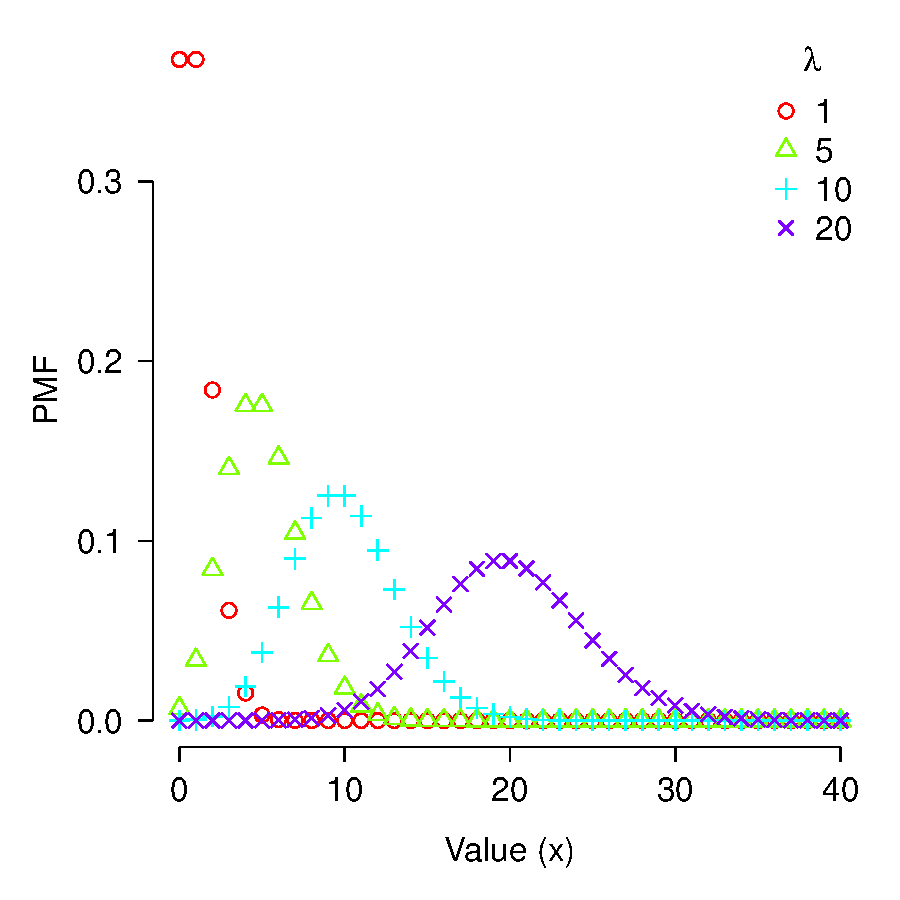
\includegraphics[keepaspectratio]{chapters/ch09_files/figure-pdf/unnamed-chunk-26-1.pdf}}
\end{center}

\subsection{Negative binomial distribution}\label{sec-dist-negbin}

The \textbf{negative binomial distribution} as usually used in biology
is used for counts that are \textbf{overdispersed}--that is, they have a
variance greater than expected given other parameters. In this case,
that means \(\sigma^2>>\lambda\). This is \emph{very common} in
biological count data. For example, a bird species might have low
abundance (0 to 4) at most sites in a study, but very high abundance (30
to 40) at a handful of sites. In that case using the Poisson
distribution would not be appropriate because doing so would mean
assuming that the variance was approximately equal to the mean when it
really wasn't.

The definition that is not used as commonly in biology is actually the
original definition: the negative binomial distribution also describes
the number of failures that occur in a series of Bernoulli trials until
some predetermined number of successes is observed. For example, when
flipping a fair coin, how many times should you expect to see tails
before you observe 8 heads? This definition is, therefore, a discrete
version of the \href{@sec-dist-gamma}{gamma distribution}. This also
makes the original definition of the negative binomial similar to the
geometric distribution (Section~\ref{sec-dist-geom}).

The version of the negative binomial that biologists use is
parameterized by its mean \(\mu\) and its overdispersion \(k\). This
definition views the negative binomial as a Poisson distribution with
parameter \(\lambda\), where \(\lambda\) itself is a random variable
that follows a Gamma distribution (Section~\ref{sec-dist-gamma}). For
this reason, some authors refer to the negative binomial as a
\textbf{Gamma-Poisson mixture distribution}. A mixture distribution is
exactly what it sounds like: a distribution that is formed by ``mixing''
or combining two distributions. Often a mixture is formed by having
parameters of one distribution vary according to another distribution.

The overdispersion parameter \(k\) is called \texttt{size} in the R
functions that work with the negative binomial. Counterintuitively, the
overdispersion in a negative binomial distribution gets larger as \(k\)
becomes smaller. This is seen in the expression for the variance of a
negative binomial distribution:

\[Var\left(X\right)=\mu+\frac{\mu^2}{k}\]

As \(k\) becomes large, the ratio \(\mu^2/k\) becomes small and
approaches 0, and thus \(Var(x)\) approaches \(\mu\). This means that a
negative binomial distribution with large \(k\) approximates a Poisson
distribution. As \(k\) approaches 0, the ratio \(\mu^2/k\) becomes
larger, and thus \(Var(x)\) increases to be much larger than \(\mu\).

\subsubsection{Negative binomial distribution in
R}\label{sec-dist-negbin-r}

The negative binomial distribution is accessed using the
\texttt{\_nbinom} group of functions, where the space could be
\texttt{d}, \texttt{p}, \texttt{q}, or \texttt{r}. These functions
calculate or returns something different:

\begin{itemize}
\tightlist
\item
  \texttt{dnbinom()}: Calculates PMF at \emph{x}. Answers the question,
  ``what is the probability of observing a count of \emph{x}?''
\item
  \texttt{pnbinom()}: Calculates CDF, or integral of PMF, from 0 up to
  \emph{x}. In other words, given some negative binomial distribution,
  at what quantile of that distribution should some value fall? The
  reverse of \texttt{qnbinom()}.
\item
  \texttt{qnbinom()}: Calculates the value at specified quantile of a
  Poisson distribution. The reverse of \texttt{pnbinom()}.
\item
  \texttt{rnbinom()}: Draws random numbers from the negative binomial
  distribution.
\end{itemize}

The R functions for the negative binomial distribution can work with
either parameterization (waiting time or mean with overdispersion). Some
of the argument names are used for both methods. If you are working with
the negative binomial distribution in R you \emph{need to name your
arguments to make sure you get the version of the negative binomial that
you want}.

The figure below shows the effect of different overdispersion
parameters. Notice that as \(k\) increases, the distribution looks more
and more like a Poisson distribution with \(\lambda = 10\). As \(k\)
gets smaller, the distribution gets more and more concentrated near 0,
and more and more right-skewed.

\begin{Shaded}
\begin{Highlighting}[]
\NormalTok{xp }\OtherTok{\textless{}{-}} \DecValTok{0}\SpecialCharTok{:}\DecValTok{30}
\NormalTok{y1 }\OtherTok{\textless{}{-}} \FunctionTok{dpois}\NormalTok{(xp, }\DecValTok{10}\NormalTok{)}
\NormalTok{y2 }\OtherTok{\textless{}{-}} \FunctionTok{dnbinom}\NormalTok{(xp, }\AttributeTok{size=}\FloatTok{0.2}\NormalTok{, }\AttributeTok{mu=}\DecValTok{10}\NormalTok{)}
\NormalTok{y3 }\OtherTok{\textless{}{-}} \FunctionTok{dnbinom}\NormalTok{(xp, }\AttributeTok{size=}\FloatTok{0.5}\NormalTok{, }\AttributeTok{mu=}\DecValTok{10}\NormalTok{)}
\NormalTok{y4 }\OtherTok{\textless{}{-}} \FunctionTok{dnbinom}\NormalTok{(xp, }\AttributeTok{size=}\DecValTok{1}\NormalTok{, }\AttributeTok{mu=}\DecValTok{10}\NormalTok{)}
\NormalTok{y5 }\OtherTok{\textless{}{-}} \FunctionTok{dnbinom}\NormalTok{(xp, }\AttributeTok{size=}\DecValTok{10}\NormalTok{, }\AttributeTok{mu=}\DecValTok{10}\NormalTok{)}
\NormalTok{y6 }\OtherTok{\textless{}{-}} \FunctionTok{dnbinom}\NormalTok{(xp, }\AttributeTok{size=}\DecValTok{50}\NormalTok{, }\AttributeTok{mu=}\DecValTok{10}\NormalTok{)}
\NormalTok{y7 }\OtherTok{\textless{}{-}} \FunctionTok{dnbinom}\NormalTok{(xp, }\AttributeTok{size=}\DecValTok{100}\NormalTok{, }\AttributeTok{mu=}\DecValTok{10}\NormalTok{)}

\NormalTok{cols }\OtherTok{\textless{}{-}} \FunctionTok{rainbow}\NormalTok{(}\DecValTok{6}\NormalTok{)}
\FunctionTok{par}\NormalTok{(}\AttributeTok{mfrow=}\FunctionTok{c}\NormalTok{(}\DecValTok{1}\NormalTok{,}\DecValTok{1}\NormalTok{), }\AttributeTok{mar=}\FunctionTok{c}\NormalTok{(}\FloatTok{5.1}\NormalTok{, }\FloatTok{5.1}\NormalTok{, }\FloatTok{1.1}\NormalTok{, }\FloatTok{1.1}\NormalTok{),}
    \AttributeTok{las=}\DecValTok{1}\NormalTok{, }\AttributeTok{bty=}\StringTok{"n"}\NormalTok{, }\AttributeTok{lend=}\DecValTok{1}\NormalTok{,}
    \AttributeTok{cex.lab=}\FloatTok{1.3}\NormalTok{, }\AttributeTok{cex.axis=}\FloatTok{1.3}\NormalTok{)}
\FunctionTok{plot}\NormalTok{(xp, y1, }\AttributeTok{pch=}\DecValTok{17}\NormalTok{, }\AttributeTok{ylim=}\FunctionTok{c}\NormalTok{(}\DecValTok{0}\NormalTok{, }\FloatTok{0.5}\NormalTok{), }\AttributeTok{xlab=}\StringTok{"X"}\NormalTok{, }\AttributeTok{ylab=}\StringTok{"PMF"}\NormalTok{)}
\FunctionTok{points}\NormalTok{(xp, y2, }\AttributeTok{pch=}\DecValTok{16}\NormalTok{, }\AttributeTok{col=}\NormalTok{cols[}\DecValTok{1}\NormalTok{])}
\FunctionTok{points}\NormalTok{(xp, y3, }\AttributeTok{pch=}\DecValTok{16}\NormalTok{, }\AttributeTok{col=}\NormalTok{cols[}\DecValTok{2}\NormalTok{])}
\FunctionTok{points}\NormalTok{(xp, y4, }\AttributeTok{pch=}\DecValTok{16}\NormalTok{, }\AttributeTok{col=}\NormalTok{cols[}\DecValTok{3}\NormalTok{])}
\FunctionTok{points}\NormalTok{(xp, y5, }\AttributeTok{pch=}\DecValTok{16}\NormalTok{, }\AttributeTok{col=}\NormalTok{cols[}\DecValTok{4}\NormalTok{])}
\FunctionTok{points}\NormalTok{(xp, y6, }\AttributeTok{pch=}\DecValTok{16}\NormalTok{, }\AttributeTok{col=}\NormalTok{cols[}\DecValTok{5}\NormalTok{])}
\FunctionTok{points}\NormalTok{(xp, y7, }\AttributeTok{pch=}\DecValTok{16}\NormalTok{, }\AttributeTok{col=}\NormalTok{cols[}\DecValTok{6}\NormalTok{])}
\FunctionTok{legend}\NormalTok{(}\StringTok{"topright"}\NormalTok{, }
\AttributeTok{legend=}\FunctionTok{c}\NormalTok{(}\StringTok{"Poisson"}\NormalTok{, }\StringTok{"k=0.2"}\NormalTok{, }\StringTok{"k=0.5"}\NormalTok{, }\StringTok{"k=1"}\NormalTok{, }\StringTok{"k=10"}\NormalTok{, }
\StringTok{"k=50"}\NormalTok{, }\StringTok{"k=100"}\NormalTok{),}
     \AttributeTok{pch=}\FunctionTok{c}\NormalTok{(}\DecValTok{17}\NormalTok{, }\FunctionTok{rep}\NormalTok{(}\DecValTok{16}\NormalTok{,}\DecValTok{6}\NormalTok{)), }\AttributeTok{col=}\FunctionTok{c}\NormalTok{(}\StringTok{"black"}\NormalTok{, cols))}
\end{Highlighting}
\end{Shaded}

\begin{center}
\pandocbounded{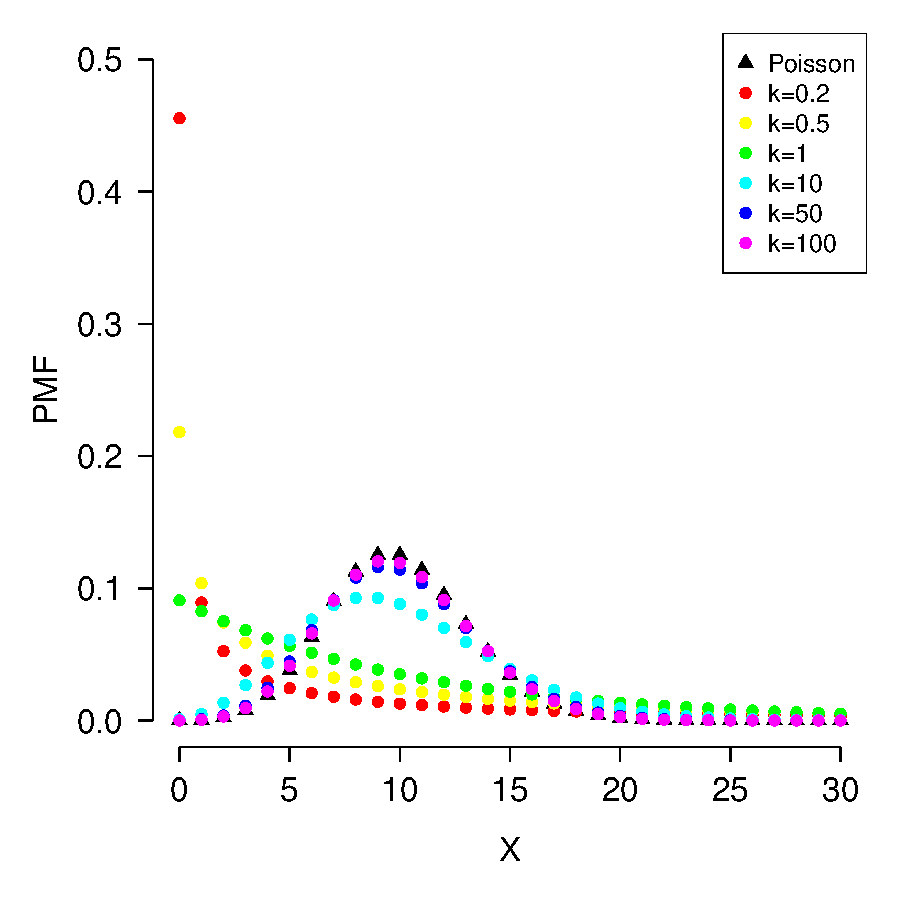
\includegraphics[keepaspectratio]{chapters/ch09_files/figure-pdf/unnamed-chunk-27-1.pdf}}
\end{center}

\subsection{Geometric distribution}\label{sec-dist-geom}

The \textbf{geometric distribution} describes the number of failures
that are seen before observing the first success, given that the
probability remains constant. It is thus related to the
\href{@sec-dist-binom}{binomial} and \href{@sec-dist-negbin}{negative
binomial}. In fact, the geometric distribution is a special case of the
negative binomial, with the number of successes = 1. The geometric
distribution is the discrete version of the
\href{@sec-dist-expo}{exponential distribution}.

The geometric distribution arises in biology when modeling waiting times
or life spans in discrete time steps. For example, if an animal has a
constant annual mortality rate, the geometric distribution models the
number of years that an individual organism completes before dying. Age-
or stage-based population matrix models such as Leslie matrices are
common in wildlife and fisheries management, and are based on annual
monitoring data. So, it makes sense to use a discrete distribution to
model survival in yearly time steps rather than continuous time. Another
biological example of when to use a geometric distribution would be
counting the number of generations until a mutation in a cell line
occurs, if mutations occur at a constant rate per generation.

Imagine a fish that has a 5\% probability of dying each year (i.e., a
95\% annual survival rate). If \(X\) is the number of complete years the
fish survives before dying, then \(X\) follows a geometric distribution
with \(p=0.05\). Let's simulate a cohort of 100,000 fish to see what
this looks like.

\begin{Shaded}
\begin{Highlighting}[]
\CommentTok{\# set annual mortality rate}
\NormalTok{P }\OtherTok{\textless{}{-}} \FloatTok{0.05}

\CommentTok{\# simulate 100000 fish}
\NormalTok{fish }\OtherTok{\textless{}{-}} \FunctionTok{rgeom}\NormalTok{(}\FloatTok{1e5}\NormalTok{, P)}

\CommentTok{\# plot the resulting lifespans}
\NormalTok{use.breaks }\OtherTok{\textless{}{-}} \FunctionTok{seq}\NormalTok{(}\SpecialCharTok{{-}}\FloatTok{0.5}\NormalTok{, }\FunctionTok{max}\NormalTok{(fish)}\SpecialCharTok{+}\FloatTok{0.5}\NormalTok{, }\AttributeTok{by=}\DecValTok{1}\NormalTok{)}
\FunctionTok{hist}\NormalTok{(fish, }\AttributeTok{breaks=}\NormalTok{use.breaks, }\AttributeTok{freq=}\ConstantTok{FALSE}\NormalTok{, }\AttributeTok{xlim=}\FunctionTok{c}\NormalTok{(}\DecValTok{0}\NormalTok{, }\DecValTok{80}\NormalTok{),}
     \AttributeTok{xlab=}\StringTok{"Years survived before death"}\NormalTok{)}
\end{Highlighting}
\end{Shaded}

\pandocbounded{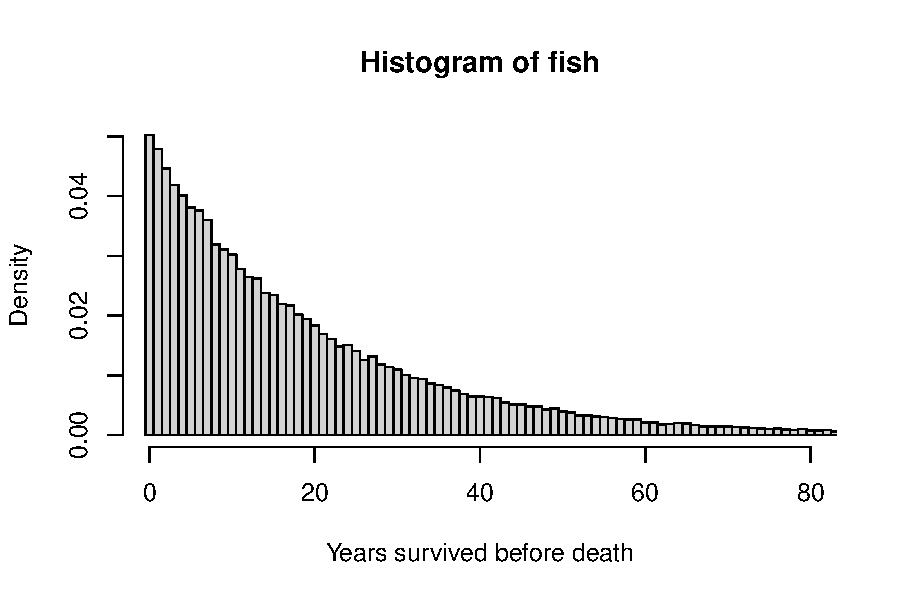
\includegraphics[keepaspectratio]{chapters/ch09_files/figure-pdf/unnamed-chunk-28-1.pdf}}

Notice that the distribution of simulated fish lifespans has a long
right tail: there are many small values, and a few very large values. We
also call this \textbf{right skewed}. Practically, this means that while
the median lifespan is 13 years, the average fish lives to 19. The long
tail pulls the arithmetic mean upwards.

\begin{Shaded}
\begin{Highlighting}[]
\CommentTok{\# by what age do 50\% of fish die?}
\FunctionTok{median}\NormalTok{(fish)}
\end{Highlighting}
\end{Shaded}

\begin{verbatim}
[1] 13
\end{verbatim}

\begin{Shaded}
\begin{Highlighting}[]
\CommentTok{\# how long does the "average" fish live?}
\FunctionTok{mean}\NormalTok{(fish)}
\end{Highlighting}
\end{Shaded}

\begin{verbatim}
[1] 19.07688
\end{verbatim}

Compare our simulation to the theoretical distribution:

\begin{Shaded}
\begin{Highlighting}[]
\NormalTok{X }\OtherTok{\textless{}{-}} \DecValTok{0}\SpecialCharTok{:}\FunctionTok{max}\NormalTok{(fish)}

\NormalTok{pmf }\OtherTok{\textless{}{-}} \FunctionTok{dgeom}\NormalTok{(X, P)}
\FunctionTok{hist}\NormalTok{(fish, }\AttributeTok{breaks=}\NormalTok{use.breaks, }\AttributeTok{freq=}\ConstantTok{FALSE}\NormalTok{, }\AttributeTok{xlim=}\FunctionTok{c}\NormalTok{(}\DecValTok{0}\NormalTok{, }\DecValTok{80}\NormalTok{),}
     \AttributeTok{xlab=}\StringTok{"Years survived before death"}\NormalTok{,}
     \AttributeTok{ylim=}\FunctionTok{c}\NormalTok{(}\DecValTok{0}\NormalTok{, }\FloatTok{0.05}\NormalTok{), }
     \AttributeTok{main=}\StringTok{"Simulated vs. theoretical distribution"}\NormalTok{)}
\FunctionTok{points}\NormalTok{(X,pmf, }\AttributeTok{type=}\StringTok{"s"}\NormalTok{, }\AttributeTok{lwd=}\DecValTok{2}\NormalTok{, }\AttributeTok{col=}\StringTok{"red"}\NormalTok{)}
\NormalTok{meanfish }\OtherTok{\textless{}{-}} \FunctionTok{round}\NormalTok{(}\FunctionTok{mean}\NormalTok{(fish),}\DecValTok{0}\NormalTok{)}
\FunctionTok{segments}\NormalTok{(meanfish, }\DecValTok{0}\NormalTok{, meanfish, }\FunctionTok{dgeom}\NormalTok{(meanfish,P),}
         \AttributeTok{lwd=}\DecValTok{2}\NormalTok{, }\AttributeTok{col=}\StringTok{"blue"}\NormalTok{)}
\CommentTok{\# calculate theoretical mean {-} matches simulation}
\NormalTok{theomean }\OtherTok{\textless{}{-}}\NormalTok{ (}\DecValTok{1}\SpecialCharTok{{-}}\NormalTok{P)}\SpecialCharTok{/}\NormalTok{P}
\FunctionTok{segments}\NormalTok{(theomean, }\DecValTok{0}\NormalTok{, theomean, }\FunctionTok{dgeom}\NormalTok{(theomean,P),}
         \AttributeTok{lwd=}\DecValTok{2}\NormalTok{, }\AttributeTok{lty=}\DecValTok{2}\NormalTok{, }\AttributeTok{col=}\StringTok{"black"}\NormalTok{)}
\end{Highlighting}
\end{Shaded}

\begin{center}
\pandocbounded{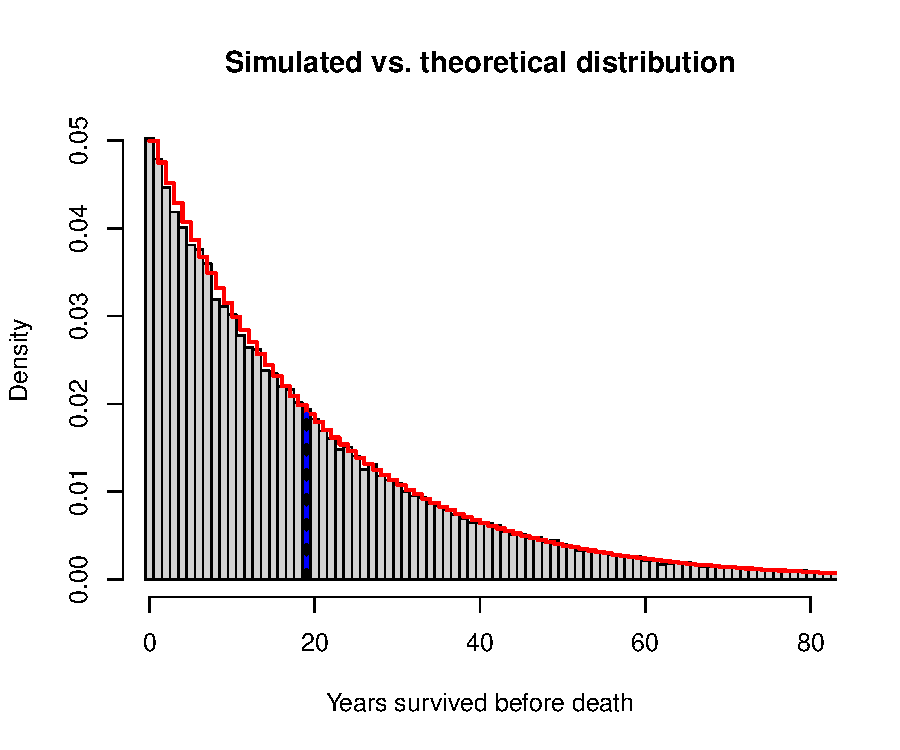
\includegraphics[keepaspectratio]{chapters/ch09_files/figure-pdf/unnamed-chunk-31-1.pdf}}
\end{center}

The figure shows that the probability of living to any given age falls
off quickly at first, then more gradually as time goes on. We can also
answer questions like ``What is the probability that a fish lives to at
least 30 years old?

\begin{Shaded}
\begin{Highlighting}[]
\CommentTok{\# answer based on simulation}
\CommentTok{\# off a bit because of sampling variation}
\FunctionTok{length}\NormalTok{(}\FunctionTok{which}\NormalTok{(fish }\SpecialCharTok{\textgreater{}=} \DecValTok{30}\NormalTok{)) }\SpecialCharTok{/} \FunctionTok{length}\NormalTok{(fish)}
\end{Highlighting}
\end{Shaded}

\begin{verbatim}
[1] 0.21554
\end{verbatim}

\begin{Shaded}
\begin{Highlighting}[]
\CommentTok{\# answer based on distribution:}
\FunctionTok{pgeom}\NormalTok{(}\DecValTok{29}\NormalTok{, P, }\AttributeTok{lower.tail=}\ConstantTok{FALSE}\NormalTok{)}
\end{Highlighting}
\end{Shaded}

\begin{verbatim}
[1] 0.2146388
\end{verbatim}

Or equivalently:

\begin{Shaded}
\begin{Highlighting}[]
\NormalTok{(}\DecValTok{1}\SpecialCharTok{{-}}\NormalTok{P)}\SpecialCharTok{\^{}}\DecValTok{30}
\end{Highlighting}
\end{Shaded}

\begin{verbatim}
[1] 0.2146388
\end{verbatim}

What age will 95\% of fish reach?

\begin{Shaded}
\begin{Highlighting}[]
\FunctionTok{qgeom}\NormalTok{(}\FloatTok{0.95}\NormalTok{, P)}
\end{Highlighting}
\end{Shaded}

\begin{verbatim}
[1] 58
\end{verbatim}

\subsection{Multinomial distribution}\label{sec-dist-multinom}

The \textbf{multinomial distribution} is a generalization of the
binomial distribution to cases with more than 2 possible outcomes. For
example, rolling a 6-sided die many times would yield a distribution of
outcomes (1, 2, 3, 4, 5, or 6) described by the multinomial
distribution. The multinomial distribution is parameterized by the
number of possible outcomes \emph{k}, the number of trials \emph{n}, and
the probabilities of each outcome \(p_1, \ldots, p_k\). The
probabilities must sum to 1.

There are some special cases of the multinomial distribution:

\begin{itemize}
\tightlist
\item
  When \(k=2\) and \(n=1\), the multinomial distribution reduces to the
  Bernoulli distribution
\item
  When \(k=2\) and \(n>1\), the multinomial distribution reduces to the
  binomial distribution
\item
  When \(k>2\) and \(n=1\), the multinomial distribution is the
  categorical distribution.
\end{itemize}

The example below shows how to work with the multinomial distribution in
R.

\begin{Shaded}
\begin{Highlighting}[]
\CommentTok{\# define 2 different sets of probabilities for}
\CommentTok{\# 5 different outcomes}
\NormalTok{p1 }\OtherTok{\textless{}{-}} \FunctionTok{c}\NormalTok{(}\FloatTok{0.2}\NormalTok{, }\FloatTok{0.2}\NormalTok{, }\FloatTok{0.1}\NormalTok{, }\FloatTok{0.1}\NormalTok{, }\FloatTok{0.4}\NormalTok{)}
\NormalTok{p2 }\OtherTok{\textless{}{-}} \FunctionTok{c}\NormalTok{(}\FloatTok{0.1}\NormalTok{, }\FloatTok{0.2}\NormalTok{, }\FloatTok{0.4}\NormalTok{, }\FloatTok{0.2}\NormalTok{, }\FloatTok{0.1}\NormalTok{)}

\CommentTok{\# sample from the multinomial distribution}
\NormalTok{N }\OtherTok{\textless{}{-}} \FloatTok{1e3}
\NormalTok{r1 }\OtherTok{\textless{}{-}} \FunctionTok{rmultinom}\NormalTok{(N, N, }\AttributeTok{prob=}\NormalTok{p1)}
\NormalTok{r2 }\OtherTok{\textless{}{-}} \FunctionTok{rmultinom}\NormalTok{(N, N, }\AttributeTok{prob=}\NormalTok{p2)}

\CommentTok{\# summarize by outcome}
\NormalTok{y1 }\OtherTok{\textless{}{-}} \FunctionTok{apply}\NormalTok{(r1, }\DecValTok{1}\NormalTok{, mean)}
\NormalTok{y2 }\OtherTok{\textless{}{-}} \FunctionTok{apply}\NormalTok{(r2, }\DecValTok{1}\NormalTok{, mean)}

\CommentTok{\# plot the results}
\FunctionTok{plot}\NormalTok{(}\DecValTok{1}\SpecialCharTok{:}\DecValTok{5}\NormalTok{, y1, }\AttributeTok{pch=}\DecValTok{16}\NormalTok{, }\AttributeTok{xlab=}\StringTok{"X"}\NormalTok{, }
     \AttributeTok{ylab=}\StringTok{"Frequency"}\NormalTok{, }\AttributeTok{ylim=}\FunctionTok{c}\NormalTok{(}\DecValTok{0}\NormalTok{, }\DecValTok{1000}\NormalTok{))}
\FunctionTok{points}\NormalTok{(}\DecValTok{1}\SpecialCharTok{:}\DecValTok{5}\NormalTok{, y2, }\AttributeTok{pch=}\DecValTok{16}\NormalTok{, }\AttributeTok{col=}\StringTok{"red"}\NormalTok{)}
\end{Highlighting}
\end{Shaded}

\begin{center}
\pandocbounded{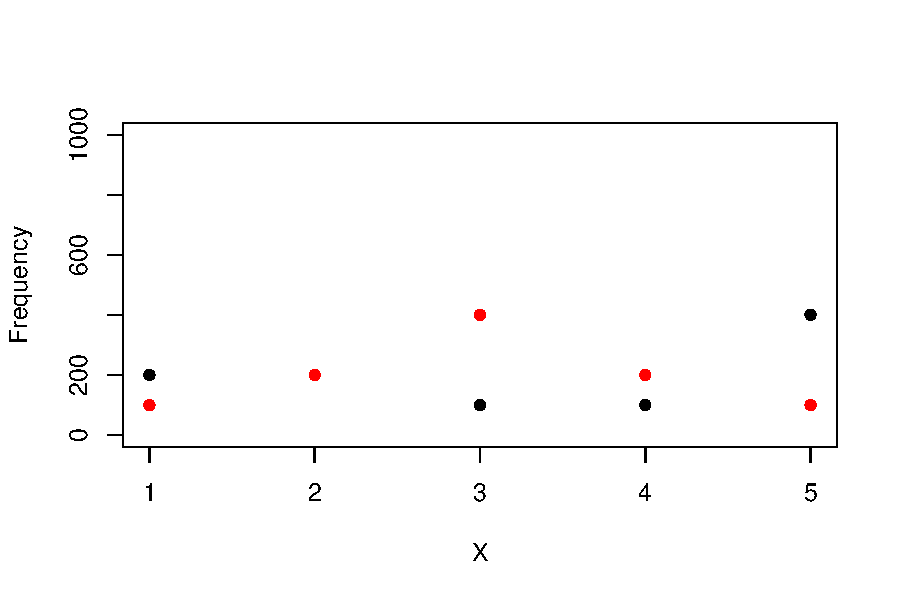
\includegraphics[keepaspectratio]{chapters/ch09_files/figure-pdf/unnamed-chunk-36-1.pdf}}
\end{center}

\section{Continuous distributions}\label{sec-dist-cont}

A \textbf{continuous distribution} can take on any real value within its
supported interval. This means that unlike discrete distributions,
continuous distributions are not restricted to integers. Measurements
like length, mass, temperature, etc., are best modeled using continuous
distributions because, although we often record them to the nearest mm,
gram, or degree, the underlying quantity varies continuously. The
apparent discreteness comes from the limited precision of our measuring
instruments.

Computing the probability of any possible outcome of a discrete
distribution is relative straightforward because there are a limited
number of outcomes. For example, a binomial distribution with \(n=10\)
and \(p=0.5\) has only 11 possible outcomes
\(\left(0,1,2,\ldots,9,10\right)\). The probabilities
\(p\left(x=0\right)\), \(p\left(x=1\right)\), and so on up to
\(p\left(x=10\right)\) must all sum to 1. The probability mass function
(PMF) of the binomial distribution at any value is the probability of
that value occurring.

This leads to an interesting question. How could we calculate the
probability of any given outcome of a distribution with an infinite
number of outcomes? If the probabilities of each individual value must
all sum to 1, and there are infinitely many possible values, then each
individual value must have probability 0. If the probability of every
possible outcome is 0, how can the distribution take on any value at
all?

To resolve this apparent contradiction, we have to take a step back and
think about what distributions really mean. The first step is to realize
that even if any single value has probability 0, an \emph{interval} of
values can have a non-zero probability. After all, the entire supported
interval of a distribution has probability 1 by definition. We can
define some interval extending from the lower limit of the distribution
up to some value \(x\). This means that for any value \(x\) in a
distribution \(X\) (note lower case vs.~upper case) we can calculate the
probability of observing a value \(\le{x}\), or
\(p\left(X\le{x}\right)\). The figure below shows this:

\begin{center}
\pandocbounded{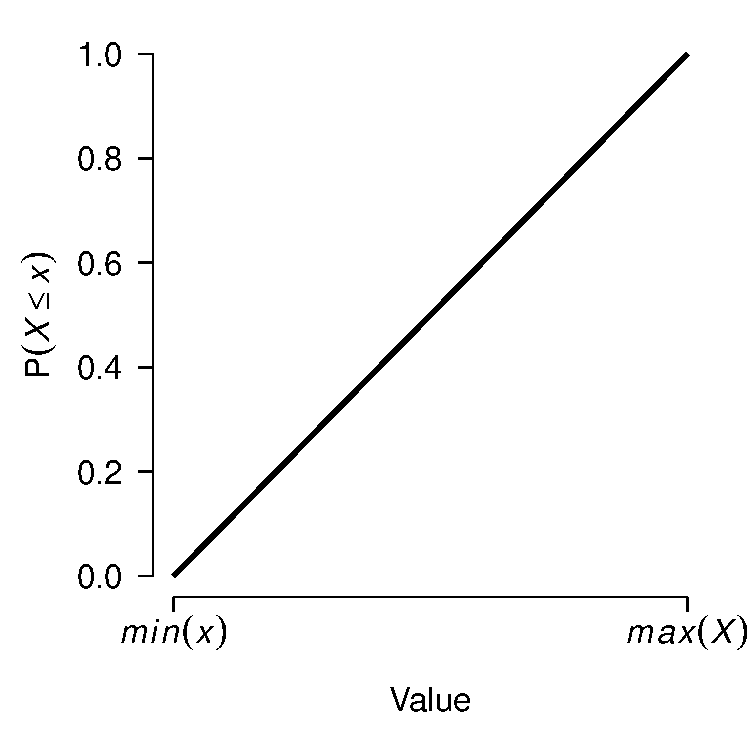
\includegraphics[keepaspectratio]{chapters/ch09_files/figure-pdf/unnamed-chunk-37-1.pdf}}
\end{center}

The \emph{y}-axis in the figure, \(P\left(X\le{x}\right)\), is called
the \textbf{cumulative distribution function (CDF)}. This name derives
from the fact that the CDF of some value \(x\) gives the cumulative or
total probability of all values up to and including \(x\). The CDF is
sometimes labeled \(F\left(x\right)\) (note the capitalized F). Another
way to interpret this is that a value \(x\) lies at the
\(CDF\left(x\right)\) quantile of a distribution. For example, if
\(CDF\left(x\right)=0.4\), then \(x\) lies at the 0.4 quantile or 40th
percentile of the distribution. Critically, this means that 40\% of the
total probability of the distribution lies at or to the left of \(x\),
and the remaining 60\% of the probability lies to the right of \(x\).

Just as the PMF describes how probability is distributed among the
possible values of a discrete random variable, the \textbf{probability
density function PDF} describes how probability is distributed over the
continuum of possible values. Although the PDF is not itself a
probability, the area under the PDF between any two values equals the
probability that the random variable falls within that interval.
Mathematically, the PDF is the rate at which the CDF changes with
respect to \(x\). That is, the PDF, \(f\left(x\right)\), is the
derivative of the CDF \(F\left(x\right)\) evaluated at \(x\):

\[f\left(x\right)=\frac{dF(x)}{dx}\]

This also means that the CDF is the integral of the PDF up to \(x\),
according to the fundamental theorem of calculus:

\[F\left(x\right)=\int_{-\infty}^{x}{f\left(x\right)\ dx}\]

In other words, probabilities correspond to areas under the PDF, while
the PDF itself represents the local density of probability. These areas
under the PDF correspond to values of the CDF.

This might be easier to see with an example. The plots below show the
PDF and CDF of a standard normal distribution with mean 0 and SD 1
(Section~\ref{sec-dist-norm}). Because the normal is unbounded, its PDF
and CDF have the domain \([-\infty,+\infty]\), but we usually truncate
the plot to a range that covers most of the CDF. For the normal, the
mean plus or minus 3 standard deviations, or \(\mu\pm{3\sigma}\), covers
over 99.7\% of values.

\begin{center}
\pandocbounded{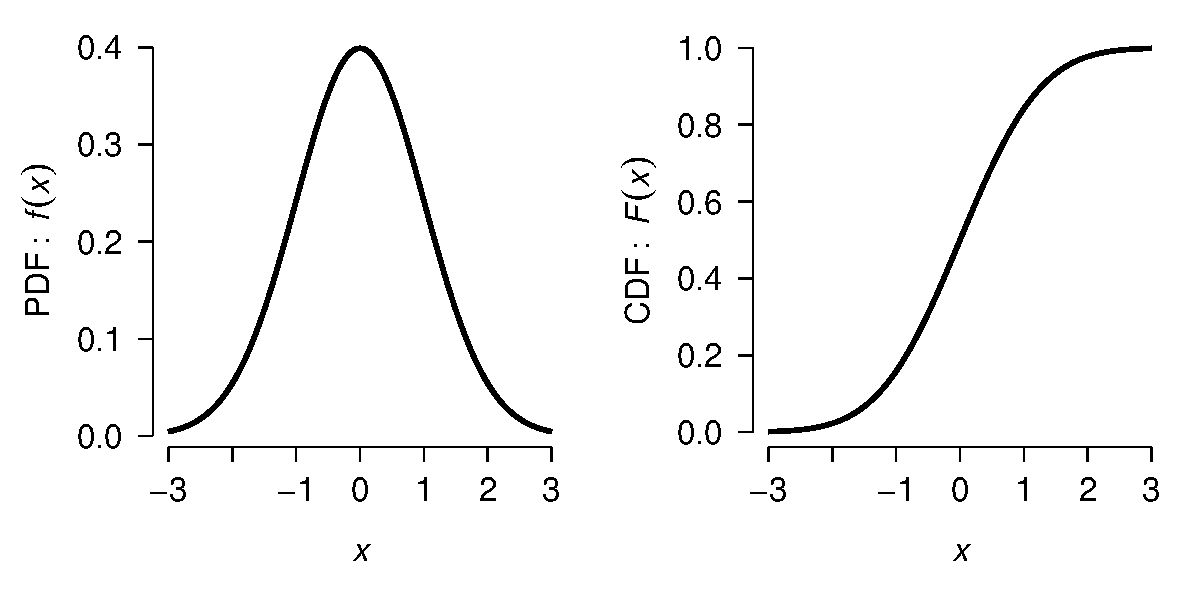
\includegraphics[keepaspectratio]{chapters/ch09_files/figure-pdf/unnamed-chunk-38-1.pdf}}
\end{center}

On the left, notice that the PDF peaks near \(x=0\) and tapers off
quickly to either side. On the right, the slope of the CDF is greatest
at \(x=0\). The value of the PDF at \(x=0\), about 0.4, is neither the
probability of observing \(x=0\) (which is 0) nor the probability of
observing \(x\le0\) (which is 0.5). The value \(f(0)=0.4\) is the rate
of change or slope in \(F(X)\) at \(x=0\).

If we wanted to calculate something like the probability of \(x=0\), we
would actually have to calculate the probability of \(x\) being in some
interval that included 0. For example, the probability that
\(-0.1\le{X}\le+0.1\), or that \(X\in\left[-1,+1\right]\), is

\[P\left(-0.1\le{X}\le+0.1\right)=F\left(0.1\right)-F\left(-0.1\right)\]

In R we can calculate:

\begin{Shaded}
\begin{Highlighting}[]
\FunctionTok{pnorm}\NormalTok{(}\FloatTok{0.1}\NormalTok{)}\SpecialCharTok{{-}}\FunctionTok{pnorm}\NormalTok{(}\SpecialCharTok{{-}}\FloatTok{0.1}\NormalTok{)}
\end{Highlighting}
\end{Shaded}

\begin{verbatim}
[1] 0.07965567
\end{verbatim}

So the probability that \(x\) is within 0.1 of 0 is about 0.08 or 8\%.
If we use a narrow interval, say \(-0.01\le{X}\le+0.01\), the
calculation becomes:

\begin{Shaded}
\begin{Highlighting}[]
\FunctionTok{pnorm}\NormalTok{(}\FloatTok{0.01}\NormalTok{)}\SpecialCharTok{{-}}\FunctionTok{pnorm}\NormalTok{(}\SpecialCharTok{{-}}\FloatTok{0.01}\NormalTok{)}
\end{Highlighting}
\end{Shaded}

\begin{verbatim}
[1] 0.007978713
\end{verbatim}

Notice that as the interval becomes narrower, its probability becomes
smaller. In the limit as the interval shrinks to a single point, the
probability becomes 0. This is why the probability of observing any
exact value in a continuous distribution is zero, even though the
probability of observing values within any finite interval is positive.

Visually, we can see this in the figure below. Notice how the red area
is much larger than the light blue area--these are the intervals defined
by \(\pm{0.1}\) and \(\pm{0.01}\).

\pandocbounded{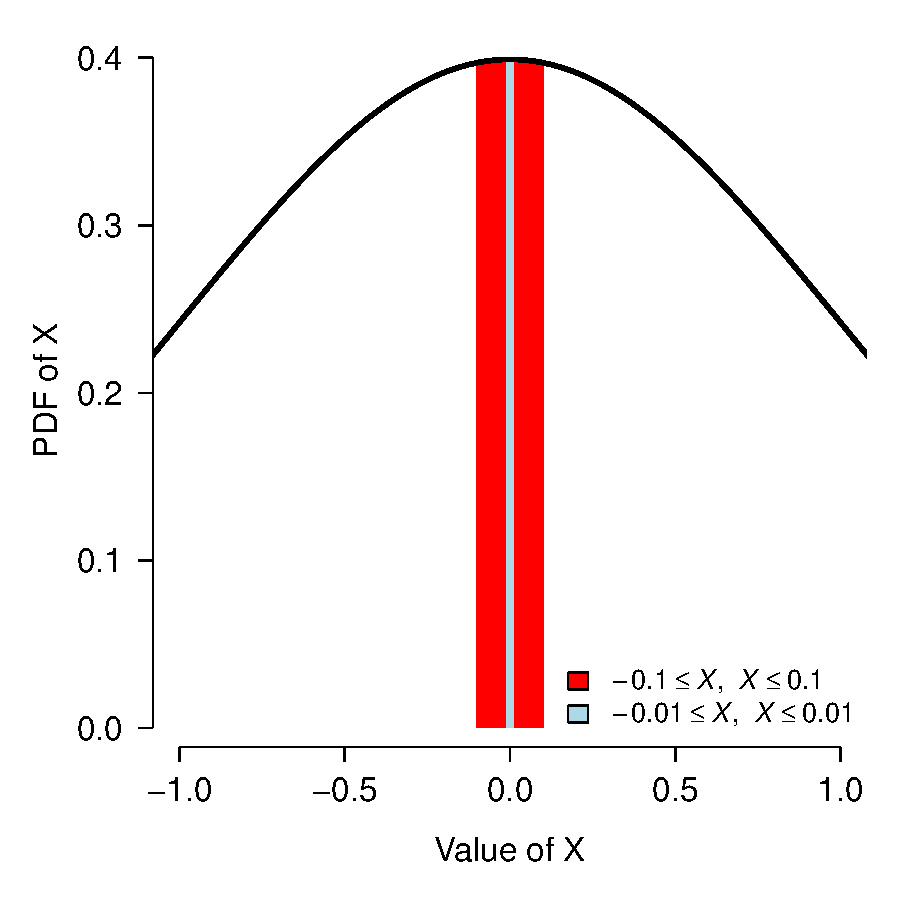
\includegraphics[keepaspectratio]{chapters/ch09_files/figure-pdf/unnamed-chunk-41-1.pdf}}

\subsection{Uniform distribution}\label{sec-dist-unif}

The simplest continuous distribution is the \textbf{uniform
distribution}. The uniform distribution is parameterized by its upper
and lower bounds, usually called \(a\) and \(b\), respectively. All
values of a uniform distribution in the interval \(\left[a,b\right]\)
are equally likely, and all values outside \(\left[a,b\right]\) have
probability 0. The figure below shows the PDFs of 3 different uniform
distributions.

\begin{center}
\pandocbounded{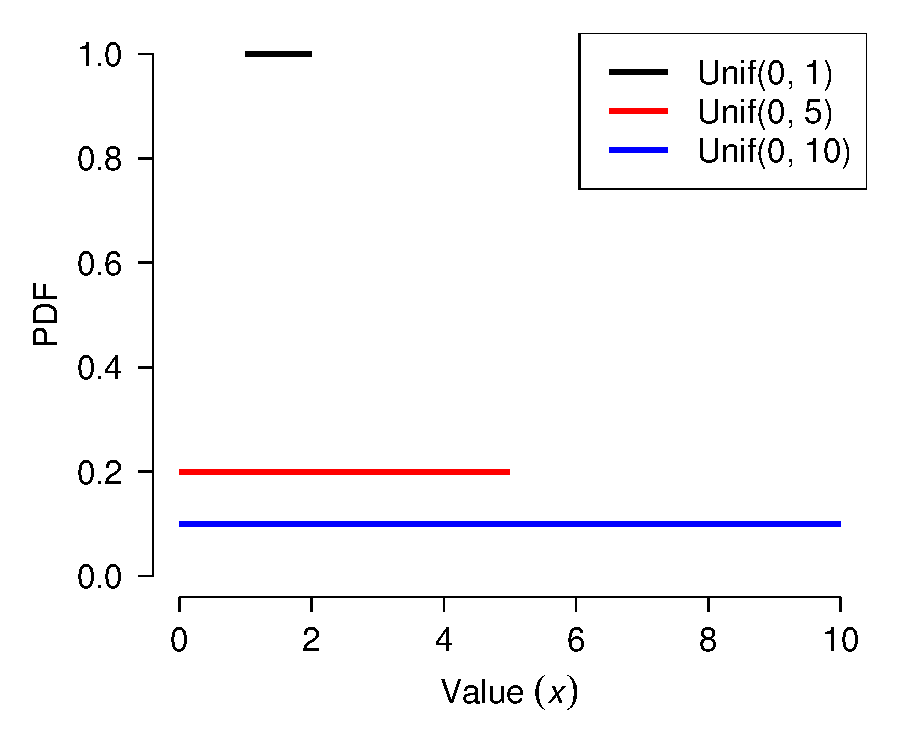
\includegraphics[keepaspectratio]{chapters/ch09_files/figure-pdf/unnamed-chunk-42-1.pdf}}
\end{center}

Notice how each distribution has a flat PDF, but that the value of the
PDF decreases as the width of the uniform distribution increases. Given
what you learned above about the relationship between the CDF and the
PDF, can you work out why this is?\footnote{The area under the PDF must
  be 1, so the height of the PDF of a uniform distribution must be 1
  divided by its width.}

Like the normal distribution, there is a standard uniform distribution
that is frequently used. The \textbf{standard uniform} is defined as
\(Uniform\left(0,1\right)\): a uniform distribution in the interval
\(\left[0,1\right]\). The uniform distribution can sometimes be
abbreviated as \(U\left(a,b\right)\) or \(Unif\left(a,b\right)\).

The mean of a uniform distribution is just the mean of its limits:

\[\mu\left(Uniform\left(a,b\right)\right)=\frac{a+b}{2}\]

The variance of a uniform distribution is:

\[\sigma^2\left(Uniform\left(a,b\right)\right)=\frac{{(b-a)}^2}{12}\]

\subsubsection{Uniform distribution in R}\label{sec-dist-unif-r}

The uniform distribution is accessed using the \texttt{\_unif} group of
functions, where the space could be \texttt{d}, \texttt{p}, \texttt{q},
or \texttt{r}. These functions calculate or returns something different:

\begin{itemize}
\tightlist
\item
  \texttt{dunif()}: Calculates probability density function (PDF) at
  \emph{x}.
\item
  \texttt{punif()}: Calculates CDF, from \emph{a} up to \emph{x}.
  Answers the question, ``at what quantile of the distribution should
  some value fall?''. The reverse of \texttt{qunif()}.
\item
  \texttt{qunif()}: Calculates the value at a specified quantile or
  quantiles. The reverse of \texttt{punif()}.
\item
  \texttt{runif()}: Draws random numbers from the uniform distribution.
\end{itemize}

The help files for many R functions include a call to \texttt{runif()}
to generate example values from the uniform distribution. This can be
confusing to new users, who might interpret ``runif'' as ``run if''
(i.e., some sort of conditional statement).

One extremely useful application is the generation of values from the
standard uniform distribution:

\begin{Shaded}
\begin{Highlighting}[]
\NormalTok{x }\OtherTok{\textless{}{-}} \FunctionTok{runif}\NormalTok{(}\DecValTok{20}\NormalTok{)}
\end{Highlighting}
\end{Shaded}

The line above generates 20 numbers from the interval {[}0, 1{]}. These
values can be used as probabilities or values of a CDF.

If you want to implement a new probability distribution in R, you can
use \texttt{runif()} followed by the \texttt{q\_\_()} function that you
define for your new distribution to implement a random number generator
for it. The example below shows how to implement a ``truncated normal''
distribution:

\begin{Shaded}
\begin{Highlighting}[]
\NormalTok{rtnorm }\OtherTok{\textless{}{-}} \ControlFlowTok{function}\NormalTok{(N, lower, upper, mu, sigma)\{}
\NormalTok{    a }\OtherTok{\textless{}{-}} \FunctionTok{pnorm}\NormalTok{(lower, mu, sigma)}
\NormalTok{    b }\OtherTok{\textless{}{-}} \FunctionTok{pnorm}\NormalTok{(upper, mu, sigma)}
\NormalTok{    x }\OtherTok{\textless{}{-}} \FunctionTok{runif}\NormalTok{(N, a, b)}
\NormalTok{    y }\OtherTok{\textless{}{-}} \FunctionTok{qnorm}\NormalTok{(x, mu, sigma)}
    \FunctionTok{return}\NormalTok{(y)}
\NormalTok{\}}

\NormalTok{use.n }\OtherTok{\textless{}{-}} \FloatTok{1e3}
\NormalTok{use.mu }\OtherTok{\textless{}{-}} \DecValTok{10}
\NormalTok{use.sd }\OtherTok{\textless{}{-}} \DecValTok{3}
\NormalTok{x1 }\OtherTok{\textless{}{-}} \FunctionTok{rnorm}\NormalTok{(use.n, use.mu, use.sd)}
\NormalTok{x2 }\OtherTok{\textless{}{-}} \FunctionTok{rtnorm}\NormalTok{(use.n, }\DecValTok{8}\NormalTok{, }\DecValTok{12}\NormalTok{, use.mu, use.sd)}

\FunctionTok{par}\NormalTok{(}\AttributeTok{mfrow=}\FunctionTok{c}\NormalTok{(}\DecValTok{1}\NormalTok{,}\DecValTok{2}\NormalTok{))}
\FunctionTok{hist}\NormalTok{(x1, }\AttributeTok{main=}\StringTok{"Normal"}\NormalTok{, }\AttributeTok{xlim=}\FunctionTok{c}\NormalTok{(}\DecValTok{0}\NormalTok{, }\DecValTok{20}\NormalTok{))}
\FunctionTok{hist}\NormalTok{(x2, }\AttributeTok{main=}\StringTok{"Truncated normal"}\NormalTok{, }\AttributeTok{xlim=}\FunctionTok{c}\NormalTok{(}\DecValTok{0}\NormalTok{, }\DecValTok{20}\NormalTok{))}
\end{Highlighting}
\end{Shaded}

\begin{center}
\pandocbounded{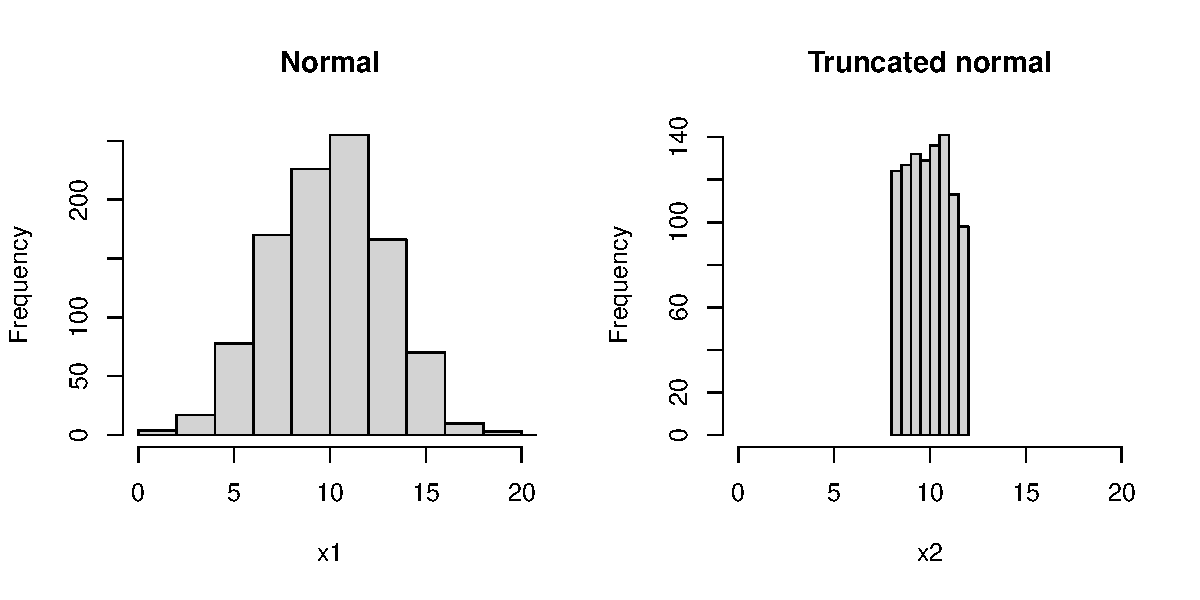
\includegraphics[keepaspectratio]{chapters/ch09_files/figure-pdf/unnamed-chunk-44-1.pdf}}
\end{center}

\subsection{Normal distribution}\label{sec-dist-norm}

The \textbf{normal distribution} is probably the most important
distribution in statistics. Many natural processes result in normal
distributions. Consequently, most classical statistical methods (e.g.,
\emph{t}-tests, ANOVA, and linear models) assume that data come from a
normal distribution. The normal distribution is also sometimes called
the \textbf{Gaussian} distribution because of the work of mathematician
Carl Friedrich Gauss, although he did not discover it.

The normal distribution is also sometimes called the \textbf{bell curve}
because of the shape of its PDF. This term should be avoided because
other probability distributions also have a bell shape, and because
normal distributions are not always bell-shaped.

The normal distribution is parameterized by its mean, \(\mu\), and
standard deviation, \(\sigma\). Some sources prefer the variance
\(\sigma^2\) instead of the standard deviation, and some even use the
precision \(1/\sigma^2\) or \(\sigma^{-2}\). This is fine because, as
the symbols imply, the SD, variance, and precision are all related. Just
pay attention to the notation being used. Using \(\sigma\) instead of
\(\sigma^2\) or \(1/\sigma^2\) can be convenient because \(\sigma\) is
in the same units as \(\mu\).

The figure below shows several normal distributions with different means
and standard deviations.

\begin{center}
\pandocbounded{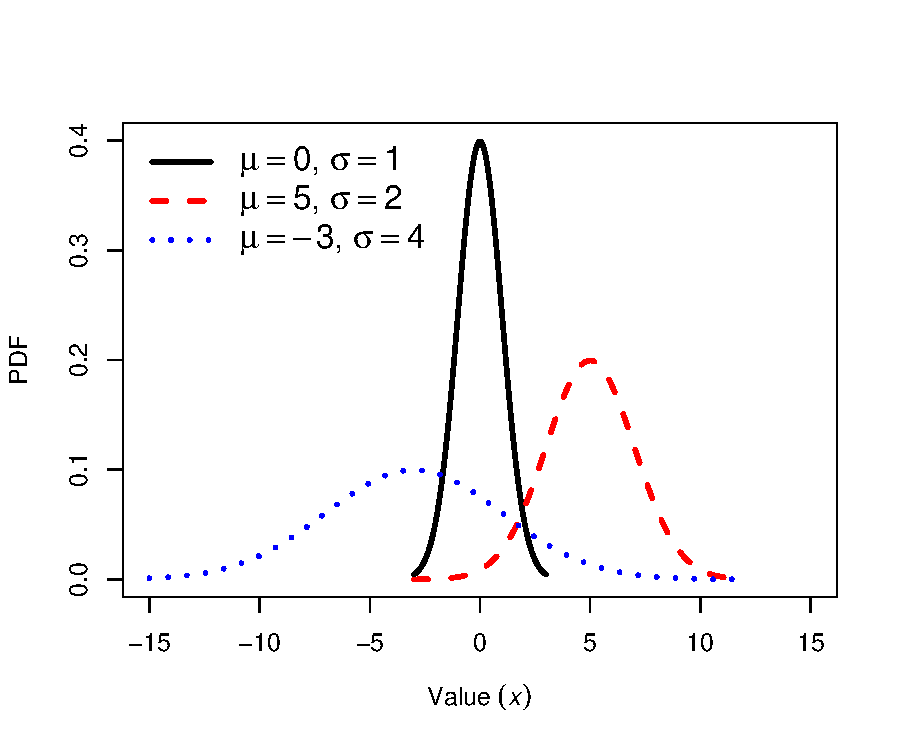
\includegraphics[keepaspectratio]{chapters/ch09_files/figure-pdf/unnamed-chunk-45-1.pdf}}
\end{center}

Many phenomena result in normal distributions because of the
\textbf{Central Limit Theorem (CLT)}. The CLT states that under certain
conditions the sum of many random variables will approximate a normal
distribution. The main condition is that the random variables will be
independent and identically distributed (often abbreviated
``\emph{i.i.d.}''). In other words, the values do not depend on each
other, but they all come from the same distribution. The exact
distribution does not matter. The example below uses the uniform
distribution. The CLT also works with the mean of the random variables
instead of the sum, because mean is just the sum scaled by sample size.

\begin{Shaded}
\begin{Highlighting}[]
\CommentTok{\# large sample size}
\NormalTok{N }\OtherTok{\textless{}{-}} \FloatTok{1e4}

\CommentTok{\# set up a vector to hold the sums of}
\CommentTok{\# the random values}
\NormalTok{xvec }\OtherTok{\textless{}{-}} \FunctionTok{numeric}\NormalTok{(N)}

\CommentTok{\# in a loop, draw 10 random values and }
\CommentTok{\# calculate their sum...10000 times}
\ControlFlowTok{for}\NormalTok{(i }\ControlFlowTok{in} \DecValTok{1}\SpecialCharTok{:}\NormalTok{N)\{xvec[i] }\OtherTok{\textless{}{-}} \FunctionTok{sum}\NormalTok{(}\FunctionTok{runif}\NormalTok{(}\DecValTok{10}\NormalTok{))\}}

\CommentTok{\# histogram of the 10000 sums}
\FunctionTok{hist}\NormalTok{(xvec)}
\end{Highlighting}
\end{Shaded}

\begin{center}
\pandocbounded{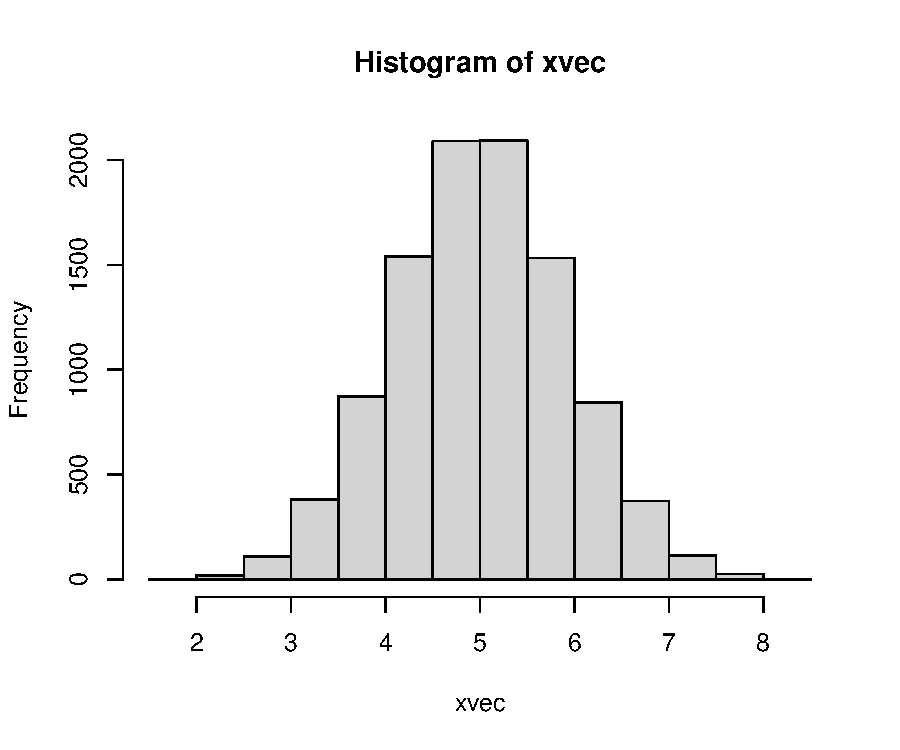
\includegraphics[keepaspectratio]{chapters/ch09_files/figure-pdf/unnamed-chunk-46-1.pdf}}
\end{center}

The \textbf{standard normal distribution} has \(\mu=0\) and
\(\sigma=1\). This is often written as \(N\left(0,1\right)\). These
parameters are the defaults in the R functions that work with the normal
distribution.

\subsubsection{Normal distribution in R}\label{sec-dist-norm-r}

The normal distribution is accessed using the \texttt{\_norm} group of
functions, where the space could be \texttt{d}, \texttt{p}, \texttt{q},
or \texttt{r}. These functions calculate or returns something different:

\begin{itemize}
\tightlist
\item
  \texttt{dnorm()}: Calculates probability density function (PDF) at
  \emph{x}.
\item
  \texttt{pnorm()}: Calculates CDF, from \(-\infty\) up to \emph{x}.
  Answers the question, ``at what quantile of the distribution should
  some value fall?''. The reverse of \texttt{qnorm()}.
\item
  \texttt{qnorm()}: Calculates the value at a specified quantile or
  quantiles. The reverse of \texttt{pnorm()}.
\item
  \texttt{rnorm()}: Draws random numbers from the normal distribution.
\end{itemize}

The normal distribution in R is parameterized by the mean (argument
\texttt{mean}) and the SD, not the variance (argument \texttt{sd}). The
figure generated below shows the effect of increasing the SD on the
shape of a distribution. Greater variance (i.e., greater SD) means that
the distribution is more spread out.

\begin{Shaded}
\begin{Highlighting}[]
\NormalTok{mu }\OtherTok{\textless{}{-}} \DecValTok{10}
\NormalTok{x }\OtherTok{\textless{}{-}} \FunctionTok{seq}\NormalTok{(}\DecValTok{0}\NormalTok{, }\DecValTok{20}\NormalTok{, }\AttributeTok{by=}\FloatTok{0.1}\NormalTok{)}
\NormalTok{y1 }\OtherTok{\textless{}{-}} \FunctionTok{dnorm}\NormalTok{(x, mu, }\DecValTok{2}\NormalTok{)}
\NormalTok{y2 }\OtherTok{\textless{}{-}} \FunctionTok{dnorm}\NormalTok{(x, mu, }\DecValTok{5}\NormalTok{)}
\NormalTok{y3 }\OtherTok{\textless{}{-}} \FunctionTok{dnorm}\NormalTok{(x, mu, }\DecValTok{10}\NormalTok{)}

\FunctionTok{par}\NormalTok{(}\AttributeTok{mfrow=}\FunctionTok{c}\NormalTok{(}\DecValTok{1}\NormalTok{,}\DecValTok{1}\NormalTok{))}
\FunctionTok{plot}\NormalTok{(x, y1, }\AttributeTok{type=}\StringTok{"l"}\NormalTok{, }\AttributeTok{lwd=}\DecValTok{3}\NormalTok{, }\AttributeTok{xlab=}\StringTok{"X"}\NormalTok{, }\AttributeTok{ylab=}\StringTok{"PDF"}\NormalTok{)}
\FunctionTok{points}\NormalTok{(x, y2, }\AttributeTok{type=}\StringTok{"l"}\NormalTok{, }\AttributeTok{lwd=}\DecValTok{3}\NormalTok{, }\AttributeTok{col=}\StringTok{"red"}\NormalTok{)}
\FunctionTok{points}\NormalTok{(x, y3, }\AttributeTok{type=}\StringTok{"l"}\NormalTok{, }\AttributeTok{lwd=}\DecValTok{3}\NormalTok{, }\AttributeTok{col=}\StringTok{"blue"}\NormalTok{)}
\FunctionTok{legend}\NormalTok{(}\StringTok{"topright"}\NormalTok{, }\AttributeTok{legend=}\FunctionTok{c}\NormalTok{(}\FunctionTok{expression}\NormalTok{(sigma}\SpecialCharTok{==}\DecValTok{2}\NormalTok{),}
        \FunctionTok{expression}\NormalTok{(sigma}\SpecialCharTok{==}\DecValTok{5}\NormalTok{), }\FunctionTok{expression}\NormalTok{(sigma}\SpecialCharTok{==}\DecValTok{10}\NormalTok{)),}
        \AttributeTok{lwd=}\DecValTok{3}\NormalTok{, }\AttributeTok{col=}\FunctionTok{c}\NormalTok{(}\StringTok{"black"}\NormalTok{, }\StringTok{"red"}\NormalTok{, }\StringTok{"blue"}\NormalTok{))}
\end{Highlighting}
\end{Shaded}

\begin{center}
\pandocbounded{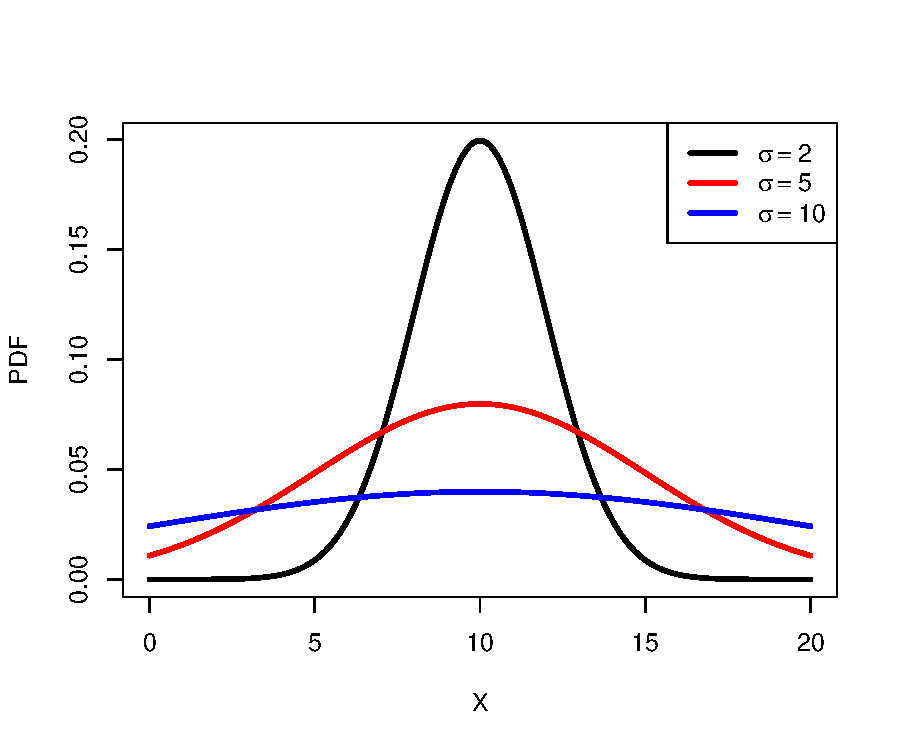
\includegraphics[keepaspectratio]{chapters/ch09_files/figure-pdf/unnamed-chunk-47-1.pdf}}
\end{center}

The normal distribution has several useful properties. Generally, the
mean and median are the same (if the distribution is not skewed).
Approximately 68\% of values fall within 1 SD of the mean, 95\% of
values fall within about 2 SD of the mean (technically 1.9599 SD, or
\texttt{qnorm(0.975)}), and 99.7\% of values fall within about 3 SD of
the mean. So, deviations of \(>3\) SD are very rare and may signify
outliers. The number of SD a value falls away from the mean is sometimes
referred to as a \textbf{\emph{z}-score} or a \textbf{sigma}.
\emph{Z}-scores are calculated as:

\[z\left(x\right)=\frac{x-\mu}{\sigma}\]

Where \emph{x} is the value, \(\mu\) is the mean, and \(\sigma\) is the
SD.

\emph{Z}-scores are sometimes used when comparing variables that are
normally distributed, but on very different scales. Converting the raw
values to their \emph{z}-scores is referred to as \textbf{standardizing}
them. Any variable, once standardized, has a mean of 0 and SD of 1. The
units of a \emph{z}-scaled variable are ``standard deviations away from
the mean''.

Standardized values are sometimes used in regression analyses in place
of raw values. Many ordination methods such as principal components
analysis (PCA) standardize variables automatically. \emph{Z}-scores (or
standardized values) are calculated in R using the \texttt{scale()}
function:

\begin{Shaded}
\begin{Highlighting}[]
\NormalTok{x1 }\OtherTok{\textless{}{-}} \FunctionTok{rnorm}\NormalTok{(}\DecValTok{100}\NormalTok{, }\DecValTok{100}\NormalTok{, }\DecValTok{40}\NormalTok{)}
\FunctionTok{par}\NormalTok{(}\AttributeTok{mfrow=}\FunctionTok{c}\NormalTok{(}\DecValTok{1}\NormalTok{,}\DecValTok{2}\NormalTok{))}
\FunctionTok{hist}\NormalTok{(x1)}
\FunctionTok{hist}\NormalTok{(}\FunctionTok{scale}\NormalTok{(x1))}
\end{Highlighting}
\end{Shaded}

\begin{center}
\pandocbounded{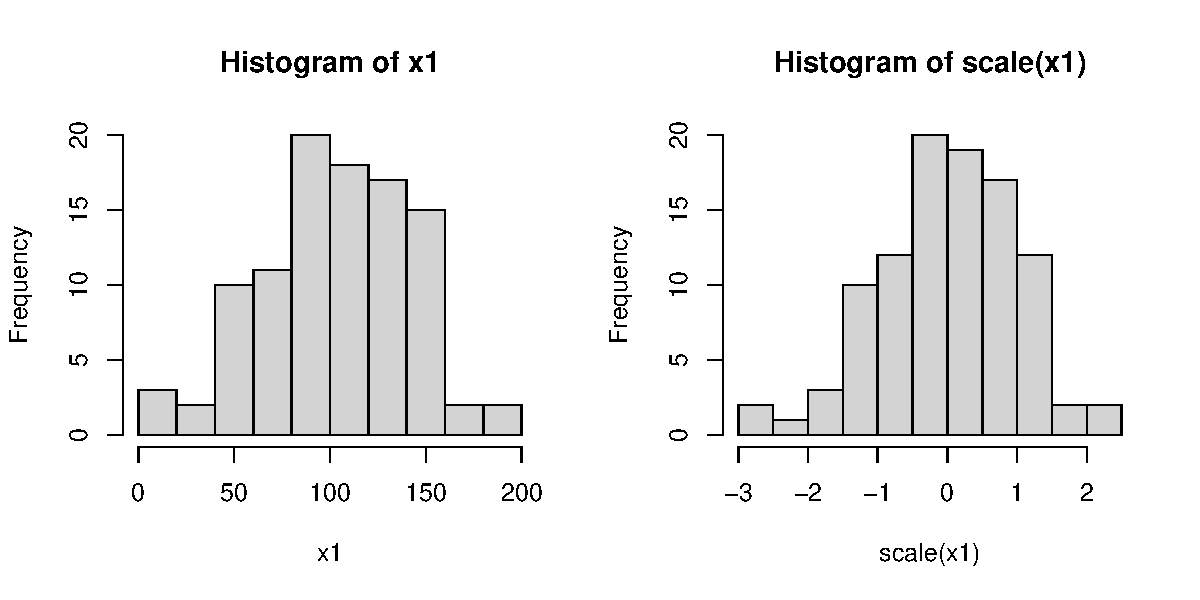
\includegraphics[keepaspectratio]{chapters/ch09_files/figure-pdf/chunkx420-1.pdf}}
\end{center}

\begin{Shaded}
\begin{Highlighting}[]
\FunctionTok{mean}\NormalTok{(x1)}
\end{Highlighting}
\end{Shaded}

\begin{verbatim}
[1] 102.6749
\end{verbatim}

\begin{Shaded}
\begin{Highlighting}[]
\FunctionTok{sd}\NormalTok{(x1)}
\end{Highlighting}
\end{Shaded}

\begin{verbatim}
[1] 39.16439
\end{verbatim}

\begin{Shaded}
\begin{Highlighting}[]
\FunctionTok{mean}\NormalTok{(}\FunctionTok{scale}\NormalTok{(x1))}
\end{Highlighting}
\end{Shaded}

\begin{verbatim}
[1] 1.765851e-16
\end{verbatim}

\begin{Shaded}
\begin{Highlighting}[]
\FunctionTok{sd}\NormalTok{(}\FunctionTok{scale}\NormalTok{(x1))}
\end{Highlighting}
\end{Shaded}

\begin{verbatim}
[1] 1
\end{verbatim}

Because standardized variables all have the same mean and SD,
standardizing a set of variables has the effect of putting all of the
variables on equal footing. Without standardizing, variables with larger
values or more variance may exert more influence on the analysis than
they should simply because of their magnitude.

\subsection{Lognormal distribution}\label{sec-dist-lnorm}

The \textbf{lognormal distribution (a.k.a.: log-normal)} is, as the name
implies, a distribution that is \emph{normal on a logarithmic scale}. If
a variable \(X\) is normally distributed and we exponentiate it, the
result \(Z=e^X\) will be lognormally distributed. Conversely, if
variable \(Z\) is lognormally distributed, then \(\log\left(Z\right)\)
will be normally distributed. By convention the \textbf{natural log}
\(\ln\), or \(\log_e\), is used to define the lognormal distribution.
R's lognormal distribution functions use the natural log scale.

The lognormal distribution arises naturally from \textbf{multiplicative}
processes. Remember that logarithms relate the operations of
multiplication and addition:

\[\log\left(ab\right)=\log\left(a\right)+\log\left(a\right)\]

Suppose some quantity \(z\) is determined by multiplying together many
positive numbers:

\[z=X_1X_2X_3\cdots X_n\]

Taking its logarithm gives:

\[\log(Z)=\log(X_1)+\log(X_2)+\log(X_3)+\cdots+\log(X_n)\]

This connects the lognormal distribution to the Central Limit Theorem
(Section~\ref{sec-dist-norm}). The ordinary CLT tells us that the sum of
many independent random contributions tends toward a normal distribution
under fairly general conditions. If a biological quantity instead
results from the product of many independent positive contributions,
then taking its logarithm converts that product into a sum.
Consequently, the logarithm of the resulting quantity can approach a
normal distribution, meaning that the original quantity approaches a
lognormal distribution.

This is relevant to many biological processes in which changes are
proportional rather than additive. For example, imagine an organism
whose size changes during each time interval by a somewhat random growth
multiplier. Its final size can be written as

\[S=S_0G_1G_2\cdots G_n\]

where each \(G_i\) is a growth multiplier applied to the starting size
\(S_0\). Small random differences in growth therefore accumulate
multiplicatively, potentially producing a lognormal distribution of
final sizes\footnote{If the growth factors \(G_n\) are constant, then
  \(S_t=S_0G^t\), or more generally an exponential function
  \(f\left(t\right)=ae^{bt}\). Attempting to calculate the derivative of
  this function leads to preferring Euler's constant \(e\) as the base
  because the function \(e^t\) is it's own derivative. Here is a
  \href{https://www.youtube.com/watch?v=m2MIpDrF7Es}{youtube video} that
  explains this visually.}.

We can demonstrate the same idea with a simulation. Suppose we
repeatedly draw 10 random positive values and multiply them together:

\begin{Shaded}
\begin{Highlighting}[]
\CommentTok{\# big sample size (10000)}
\NormalTok{N }\OtherTok{\textless{}{-}} \FloatTok{1e4}
\CommentTok{\# set up vector for 10000 values}
\NormalTok{xvec }\OtherTok{\textless{}{-}} \FunctionTok{numeric}\NormalTok{(N)}
\CommentTok{\# in a loop, draw 10 random values in [1,2]}
\CommentTok{\# and multiply them all together...10000 times}
\ControlFlowTok{for}\NormalTok{(i }\ControlFlowTok{in} \DecValTok{1}\SpecialCharTok{:}\NormalTok{N)\{xvec[i] }\OtherTok{\textless{}{-}} \FunctionTok{prod}\NormalTok{(}\FunctionTok{runif}\NormalTok{(}\DecValTok{10}\NormalTok{, }\DecValTok{1}\NormalTok{, }\DecValTok{2}\NormalTok{))\}}

\CommentTok{\# plot a histogram of the products,}
\CommentTok{\# and histogram of the log of the products}
\FunctionTok{par}\NormalTok{(}\AttributeTok{mfrow=}\FunctionTok{c}\NormalTok{(}\DecValTok{1}\NormalTok{,}\DecValTok{2}\NormalTok{))}
\FunctionTok{hist}\NormalTok{(xvec, }\AttributeTok{xlab=}\StringTok{"Product"}\NormalTok{, }\AttributeTok{main=}\StringTok{"Original scale"}\NormalTok{)}
\FunctionTok{hist}\NormalTok{(}\FunctionTok{log}\NormalTok{(xvec), }\AttributeTok{xlab=}\StringTok{"Log(Product)"}\NormalTok{, }\AttributeTok{main=}\StringTok{"Log scale"}\NormalTok{)}
\end{Highlighting}
\end{Shaded}

\begin{center}
\pandocbounded{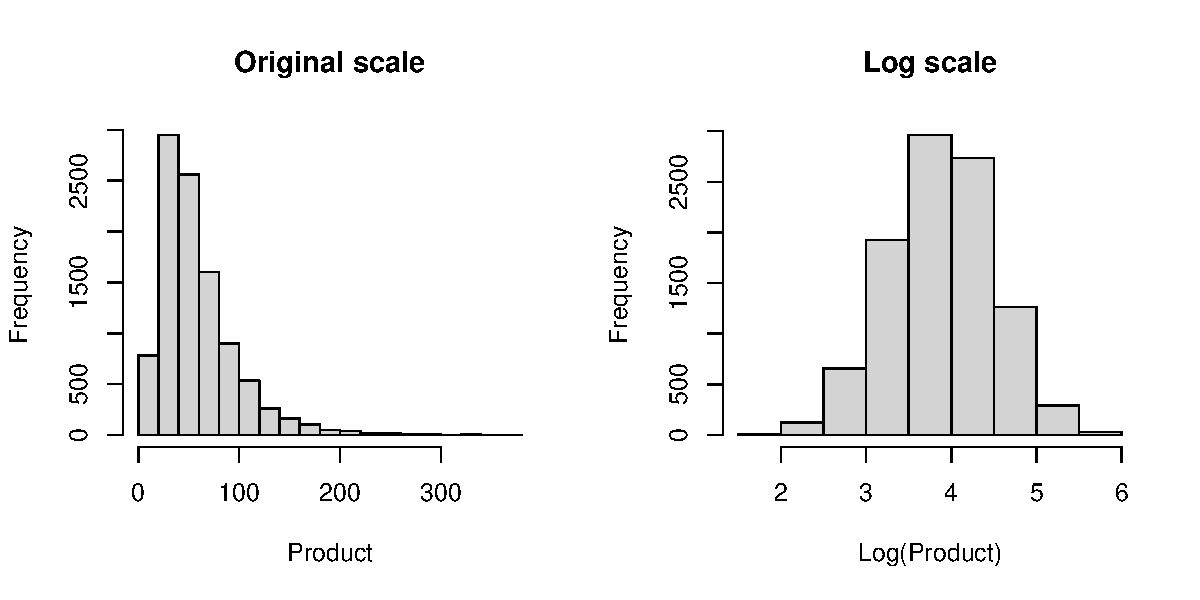
\includegraphics[keepaspectratio]{chapters/ch09_files/figure-pdf/unnamed-chunk-52-1.pdf}}
\end{center}

The products in \texttt{xvec} are strongly right skewed on their
original scale, but their logarithms are approximately normally
distributed. This happens because

\[
\log\left(\prod_{i=1}^{10} X_i\right)
=
\sum_{i=1}^{10}\log(X_i)
\] turning the multiplicative process into an additive one.

More generally, lognormal distributions are useful for describing
positive, right-skewed variables in which most observations are
relatively small but a few observations are much larger. Such patterns
are common in biological measurements including organism sizes,
abundances, concentrations, and other quantities influenced by
proportional or multiplicative processes. Other positive, right-skewed
distributions, particularly the gamma distribution
(Section~\ref{sec-dist-gamma}), can produce superficially similar
shapes, so the shape of a histogram alone does not establish that a
process is lognormal.

The lognormal distribution is parameterized by the mean and standard
deviation of the variable after taking its logarithm. In R these
parameters are named \texttt{meanlog} and \texttt{sdlog}. Thus, they are
not the mean and standard deviation of the lognormally distributed
variable on its original scale. Forgetting which quantities are on the
log scale is an easy way to produce confusing results, especially when
calculating expected values or graphing distributions.

The figure below shows various lognormal distributions with \(\mu=3\)
and different SD on a logarithmic scale (left) and a linear scale.

\begin{center}
\pandocbounded{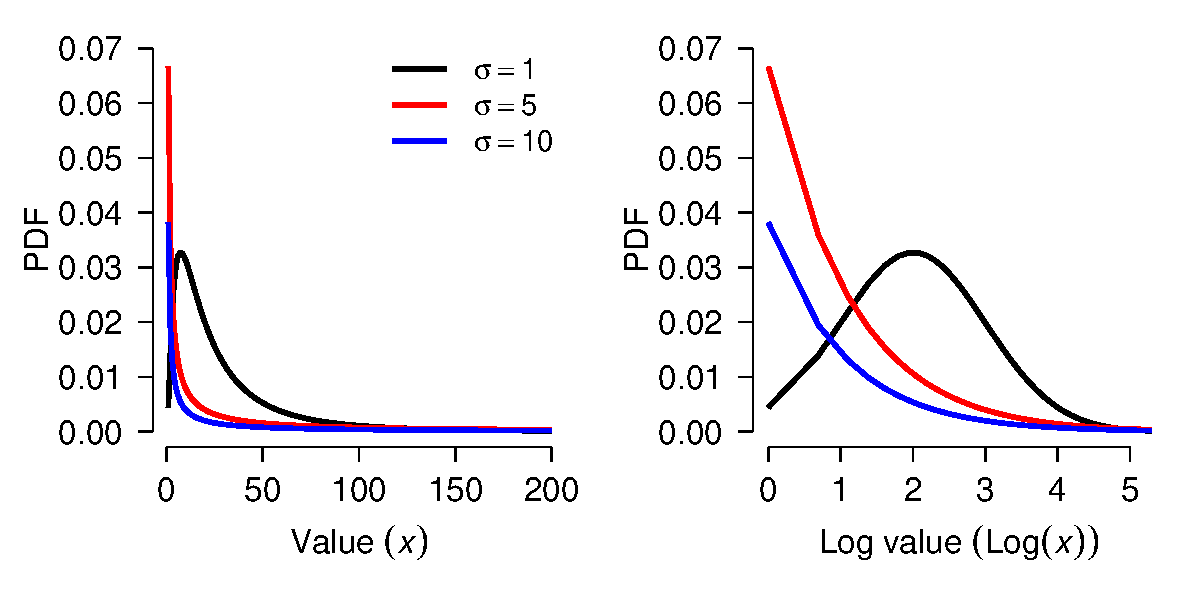
\includegraphics[keepaspectratio]{chapters/ch09_files/figure-pdf/unnamed-chunk-53-1.pdf}}
\end{center}

The figures show the effect that variance can have on the lognormal
distribution. When the variance on the log scale is \(<\mu\), the
distribution is approximately normal on the log scale. As the variance
gets larger, the distribution gets more and more right-skewed.
Right-skewed means that the values are more and more concentrated near
0, and there are fewer very large values.

Interestingly, the mean of a log-normal distribution is not simply
\(e^\mu\) as one might expect. The mean of a lognormal distribution
\emph{X} on the linear scale is

\[mean\left(X\right)=e^{\left(\frac{\mu+\sigma^2}{2}\right)}\]

In this equation, \(\mu\) and \(\sigma\) are the mean and SD on the
logarithmic scale, or \texttt{logmean} and \texttt{logsigma} in R terms.
The variance on the linear scale is:

\[Var\left(X\right)=e^{2\mu+\sigma^2}\left(e^{\sigma^2}-1\right)\]

What this means is that you cannot transform the parameters of a
lognormal distribution from the logarithmic to the linear scale by
simply exponentiating or taking logarithms of parameters.

\subsubsection{Lognormal distribution in R}\label{sec-dist-lnorm-r}

The lognormal distribution is accessed using the \texttt{\_lnorm} group
of functions, where the space could be \texttt{d}, \texttt{p},
\texttt{q}, or \texttt{r}. These functions calculate or returns
something different:

\begin{itemize}
\tightlist
\item
  \texttt{dlnorm()}: Calculates probability density function (PDF) at
  \emph{x}.
\item
  \texttt{plnorm()}: Calculates CDF, from 0 up to \emph{x}. Answers the
  question, ``at what quantile of the distribution should some value
  fall?''. The reverse of \texttt{qlnorm()}.
\item
  \texttt{qlnorm()}: Calculates the value at a specified quantile or
  quantiles. The reverse of \texttt{plnorm()}.
\item
  \texttt{rlnorm()}: Draws random numbers from the lognormal
  distribution.
\end{itemize}

When working with the lognormal distribution in R it is important to
keep in mind that the parameters (\texttt{meanlog} and \texttt{sdlog})
of the \texttt{\_lnorm} functions are on the \emph{natural log scale}.
The \texttt{meanlog} parameter is the \emph{mean of the logarithm} of
the values, not the mean of the values or the logarithm of the mean of
the values. Similarly, \texttt{sdlog} is the
\texttt{SD\ of\ the\ logarithm} of the values, not the SD of the values
or the logarithm of the SD of the values. The example below shows this:

\begin{Shaded}
\begin{Highlighting}[]
\CommentTok{\# draw some values}
\NormalTok{x1 }\OtherTok{\textless{}{-}} \FunctionTok{rlnorm}\NormalTok{(}\FloatTok{1e4}\NormalTok{, }\DecValTok{2}\NormalTok{, }\DecValTok{1}\NormalTok{)}

\CommentTok{\# mean of the values}
\FunctionTok{mean}\NormalTok{(x1)}
\end{Highlighting}
\end{Shaded}

\begin{verbatim}
[1] 12.16433
\end{verbatim}

\begin{Shaded}
\begin{Highlighting}[]
\CommentTok{\# mean of the log(values)}
\FunctionTok{mean}\NormalTok{(}\FunctionTok{log}\NormalTok{(x1))}
\end{Highlighting}
\end{Shaded}

\begin{verbatim}
[1] 1.997859
\end{verbatim}

\begin{Shaded}
\begin{Highlighting}[]
\CommentTok{\# not the log of the mean of the values}
\FunctionTok{log}\NormalTok{(}\FunctionTok{mean}\NormalTok{(x1))}
\end{Highlighting}
\end{Shaded}

\begin{verbatim}
[1] 2.498508
\end{verbatim}

\begin{Shaded}
\begin{Highlighting}[]
\CommentTok{\# sd of the values}
\FunctionTok{sd}\NormalTok{(x1)}
\end{Highlighting}
\end{Shaded}

\begin{verbatim}
[1] 16.08477
\end{verbatim}

\begin{Shaded}
\begin{Highlighting}[]
\CommentTok{\# sd of the log(values)}
\FunctionTok{sd}\NormalTok{(}\FunctionTok{log}\NormalTok{(x1))}
\end{Highlighting}
\end{Shaded}

\begin{verbatim}
[1] 0.9971798
\end{verbatim}

\begin{Shaded}
\begin{Highlighting}[]
\CommentTok{\# exp(meanlog) != mean(x1)}
\FunctionTok{c}\NormalTok{(}\FunctionTok{exp}\NormalTok{(}\DecValTok{2}\NormalTok{), }
  \FunctionTok{mean}\NormalTok{(x1))}
\end{Highlighting}
\end{Shaded}

\begin{verbatim}
[1]  7.389056 12.164334
\end{verbatim}

\subsection{Gamma distribution}\label{sec-dist-gamma}

The \textbf{gamma distribution} describes waiting times until a certain
number of events takes place. This means it is the continuous analogue
of the \href{@sec-dist-negbin}{negative binomial distribution}, which
describes the number of trials until some certain number of successes.
The gamma distribution can also be used empirically to describe positive
data whose SD is much larger than the mean. This makes it an alternative
to the lognormal distribution for right-skewed data, much like the
negative binomial is an alternative to the Poisson. Example gamma
distributions are shown below.

\begin{center}
\pandocbounded{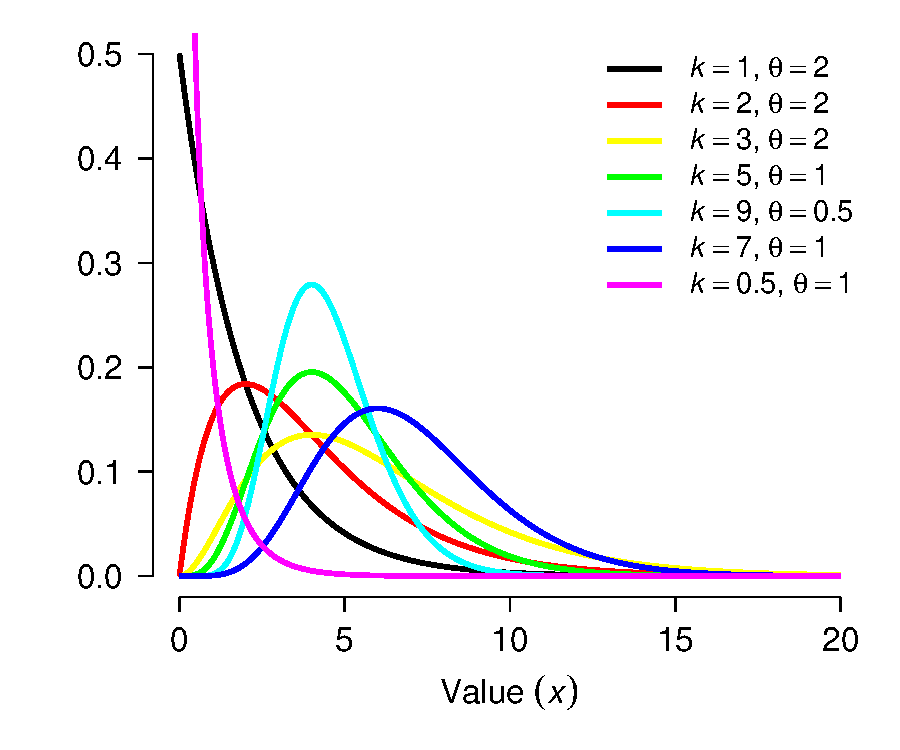
\includegraphics[keepaspectratio]{chapters/ch09_files/figure-pdf/unnamed-chunk-60-1.pdf}}
\end{center}

The Gamma distribution is parameterized by its \textbf{shape} and
\textbf{scale}.

\begin{itemize}
\tightlist
\item
  The shape parameter \(k\) describes the number of events
\item
  The scale parameter \(\theta\) (``theta'') describes the mean time
  until each event.
\item
  The scale is sometimes expressed as its reciprocal, the \textbf{rate}.
\end{itemize}

In R, the gamma can be parameterized by either the \texttt{shape} and
\texttt{scale}, or \texttt{shape} and \texttt{rate}. This means you need
to name your arguments when working with the gamma distribution.

For example, \(\Gamma(k=4,\theta=2)\) is the distribution of length of
time in days it would take to observe 4 events if events occur on
average once every two days. Equivalently, it is the time to observe 4
events if events occur at a rate of 1/2 event per day. Consequently, the
mean of a gamma distribution given shape \(k\) and scale \(\theta\) (or
rate \(r\)) is:

\[\mu=k\theta=\frac{k}{r}\]

The variance is calculated as:

\[\sigma^2=k\theta^2=\frac{k}{r^2}\]

Like the negative binomial, the gamma distribution is often used
phenomenologically; that is, used to describe a variable even if its
mechanistic description (waiting times) doesn't make sense biologically.
Just as the negative binomial can be used to model count data with
variance greater than the mean (i.e., an overdispersed Poisson), a gamma
distribution can be used for positive data with \(\sigma\gg\mu\). I.e.,
the gamma can be used in many of the same cases as the lognormal,
although the lognormal may have a clearer biological interpretation.

\subsubsection{Gamma distribution in R}\label{sec-dist-gamma-r}

The gamma distribution is accessed using the \texttt{\_gamma} group of
functions, where the space could be \texttt{d}, \texttt{p}, \texttt{q},
or \texttt{r}. These functions calculate or returns something different:

\begin{itemize}
\tightlist
\item
  \texttt{dgamma()}: Calculates probability density function (PDF) at
  \emph{x}.
\item
  \texttt{pgamma()}: Calculates CDF, from 0 up to \emph{x}. Answers the
  question, ``at what quantile of the distribution should some value
  fall?''. The reverse of \texttt{qgamma()}.
\item
  \texttt{qgamma()}: Calculates the value at a specified quantile or
  quantiles. The reverse of \texttt{pgamma()}.
\item
  \texttt{rgamma()}: Draws random numbers from the gamma distribution.
\end{itemize}

Note that when working with the gamma distribution in R, you must supply
either the \texttt{shape} and the \texttt{rate}, or the \texttt{shape}
and the \texttt{scale}. Supplying \texttt{scale} and \texttt{rate} will
return an error.

\begin{Shaded}
\begin{Highlighting}[]
\CommentTok{\# will work:}
\FunctionTok{rgamma}\NormalTok{(}\DecValTok{10}\NormalTok{, }\AttributeTok{shape=}\DecValTok{3}\NormalTok{, }\AttributeTok{scale=}\DecValTok{2}\NormalTok{)}
\FunctionTok{rgamma}\NormalTok{(}\DecValTok{10}\NormalTok{, }\AttributeTok{shape=}\DecValTok{3}\NormalTok{, }\AttributeTok{rate=}\FloatTok{0.5}\NormalTok{)}

\CommentTok{\# will return error:}
\FunctionTok{rgamma}\NormalTok{(}\DecValTok{10}\NormalTok{, }\AttributeTok{scale=}\DecValTok{2}\NormalTok{, }\AttributeTok{rate=}\FloatTok{0.5}\NormalTok{)}
\end{Highlighting}
\end{Shaded}

\subsection{Beta distribution}\label{sec-dist-beta}

The \textbf{beta distribution} is defined on the interval \([0,1]\) and
is parameterized by two positive shape parameters, \(\alpha\) and
\(\beta\). For this reason, the beta distribution is often used to model
the distribution of probabilities. The beta distribution is probably the
most commonly used distribution for variables constrained to lie between
0 and 1, such as probabilities, proportions, and fractions.

The beta distribution is closely related to the binomial distribution.
One way to think about the two shape parameters is as summaries of a
binomial trial. Parameter \(\alpha\) behaves like the number of
successes plus one, while \(\beta\) behaves like the number of failures
plus one. This interpretation provides useful intuition for the shape of
the distribution: increasing \(\alpha\) shifts probability toward 1,
while increasing \(\beta\) shifts probability toward 0. However,
\(\alpha\) and \(\beta\) are simply shape parameters and do not have to
be integers; but, they do have to be positive.

An even simpler explanation is that the balance of \(\alpha\) and
\(\beta\) determine where most of the probability lies. Increasing
\(\alpha\) places more probability near 1, whereas increasing \(\beta\)
places more probability near 0. Increasing both will crowd the
distribution near 0.5. Decreasing both will push the probability out
towards 0 and 1 and away from 0.5.

The figure below shows various beta distributions. Notice how
probability is shifted toward the center when \(\alpha\) and \(\beta\)
both increase, and how the distribution becomes U-shaped when they both
decrease.

\begin{center}
\pandocbounded{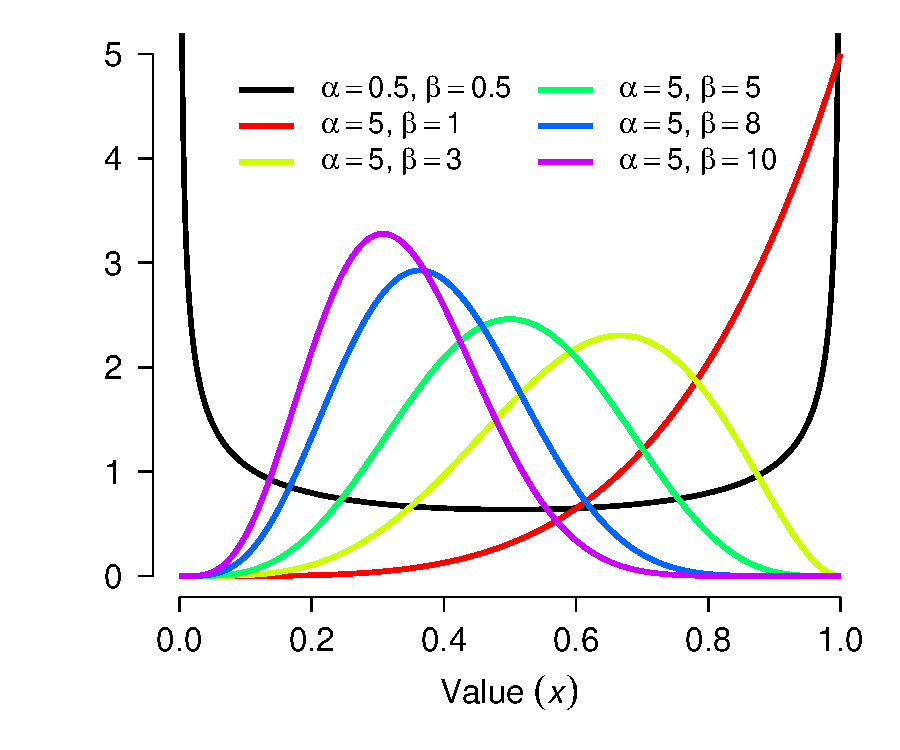
\includegraphics[keepaspectratio]{chapters/ch09_files/figure-pdf/unnamed-chunk-62-1.pdf}}
\end{center}

The beta distribution has mean

\[\mu=\frac{\alpha}{\alpha+\beta}\]

and variance

\[\sigma^2=\frac{\alpha\beta}{\left(\alpha+\beta\right)^2\left(\alpha+\beta+1\right)}\]

These expressions can be re-arranged to solve for \(\alpha\) and
\(\beta\) given a mean and variance:

\[\alpha=\left(\frac{1-\mu}{\sigma^2}-\frac{1}{\mu}\right)\mu^2\]

\[\beta=\alpha\left(\frac{1}{\mu}-1\right)\]

This is useful if you want to use proportions or percentages that were
reported as a mean and variance (or SD, or SE). For example, if a paper
reports a survival rate estimate as \(0.25\pm0.18\) SE, it's tempting to
misinterpret that as meaning that the survival rate is a
normally-distributed variable. However, treating the survival rate as
normally distributed would imply that about 8\% of the time, the
survival rate was negative!

\begin{Shaded}
\begin{Highlighting}[]
\FunctionTok{pnorm}\NormalTok{(}\DecValTok{0}\NormalTok{, }\FloatTok{0.25}\NormalTok{, }\FloatTok{0.18}\NormalTok{)}
\end{Highlighting}
\end{Shaded}

\begin{verbatim}
[1] 0.08243327
\end{verbatim}

So, you should convert these estimates to a beta distribution if you
want to understand how they might vary:

\[\alpha=\left(\frac{1-0.25}{\left(0.18\right)^2}-\frac{1}{0.25}\right){0.25}^2\approx1.1968\]

\[\beta=1.1968\left(\frac{1}{0.25}-1\right)\approx3.5903\]

The figure below shows the two distributions, the normal in black and
the beta in blue. The dashed vertical line at 0 shows that part of the
normal distribution implied by the mean and SE of a survival
``probability'' is not possible. Converting to a beta distribution
preserves the mean and variance while ensuring that all values fall
between 0 and 1. This more accurately reflects the true nature of the
uncertainty about the probability.

Note that this conversion cannot be done for some combinations of
\(\mu\) and \(\sigma\): both \(\alpha\) and \(\beta\) must both be
positive, so if you calculate a non-positive value for either parameter
then the conversion won't work. These formulas also require that

\[\sigma^2<\mu\left(1-\mu\right)\]

This can sometimes happen for probabilities very close to 0 or 1 with
large variances.

\begin{center}
\pandocbounded{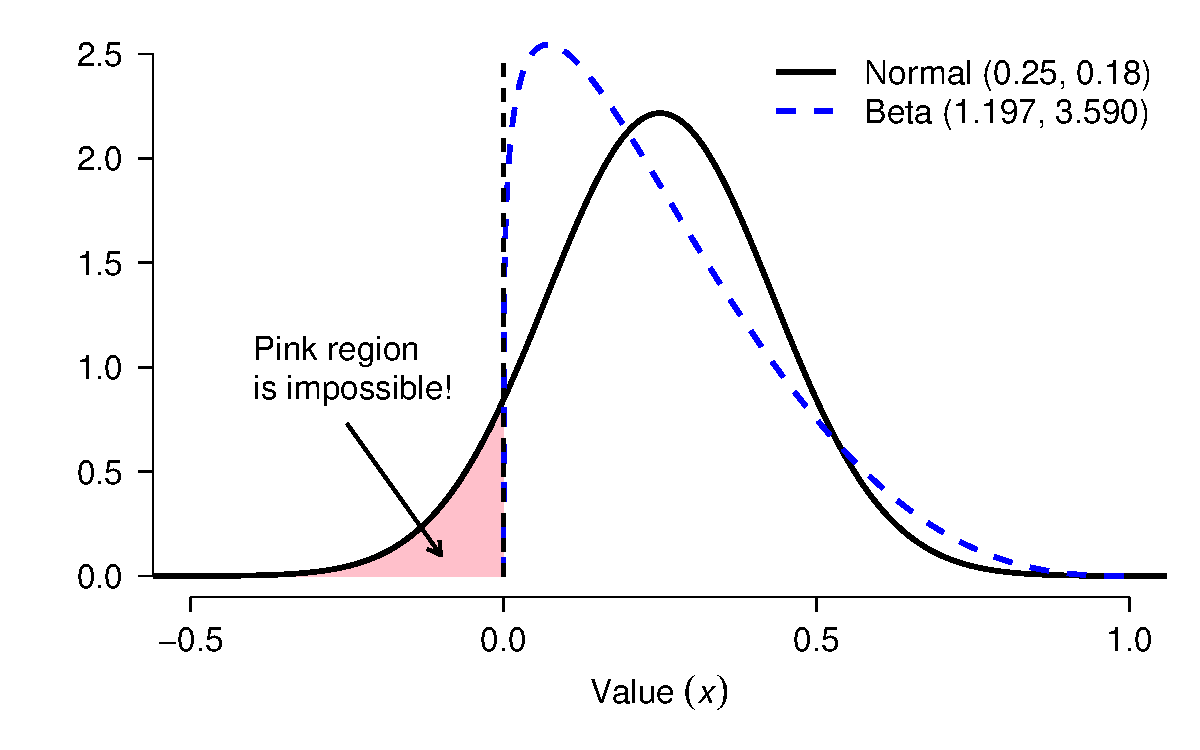
\includegraphics[keepaspectratio]{chapters/ch09_files/figure-pdf/unnamed-chunk-64-1.pdf}}
\end{center}

\subsubsection{Beta distribution in R}\label{sec-dist-beta-r}

The beta distribution is accessed using the \texttt{\_beta} group of
functions, where the space could be \texttt{d}, \texttt{p}, \texttt{q},
or \texttt{r}. These functions calculate or returns something different:

\begin{itemize}
\tightlist
\item
  \texttt{dbeta()}: Calculates probability density function (PDF) at
  \emph{x}.
\item
  \texttt{pbeta()}: Calculates CDF, from 0 up to \emph{x}. Answers the
  question, ``at what quantile of the distribution should some value
  fall?''. The reverse of \texttt{qbeta()}.
\item
  \texttt{qbeta()}: Calculates the value at a specified quantile or
  quantiles. The reverse of \texttt{pbeta()}.
\item
  \texttt{rbeta()}: Draws random numbers from the beta distribution.
\end{itemize}

\subsubsection{The beta and the binomial}\label{sec-dist-beta-binom}

The relationship between the beta and binomial distributions is
especially useful for making inferences about probabilities. The
binomial distribution describes the number of successes we observe when
the probability of success \(p\) is fixed. The beta distribution can
instead be used to describe our uncertainty about the value of \(p\)
itself.

We can take advantage of the relationship between the binomial and beta
distributions to make inferences from count data. Imagine a study where
biologists track the probability that fruit flies die before they are 3
weeks old. They report that 30 out of 130 flies die on or before day 21
of life. What can we estimate about the underlying distribution of
3-week survival rates?

One common starting point is to treat all survival probabilities between
0 and 1 as equally plausible before seeing the data. This corresponds to
\(\alpha=\beta=1\). We then add the observed successes to \(\alpha\) and
failures to \(\beta\).

Then we can model uncertainty either in the survival probability or
mortality probability, depending on how we frame successes or failures.
If survival is a success, then

\[p_{survival}\sim{Beta\left(\alpha=101,\beta=31\right)}\]

Alternatively, we can model mortality rate using mortality as a success:

\[p_{mortality}\sim{Beta\left(\alpha=31,\beta=101\right)}\]

The mean survival rate is:

\begin{Shaded}
\begin{Highlighting}[]
\NormalTok{Alpha }\OtherTok{\textless{}{-}} \DecValTok{101}
\NormalTok{Beta }\OtherTok{\textless{}{-}} \DecValTok{31}

\CommentTok{\# mean estimated survival probability}
\NormalTok{Alpha }\SpecialCharTok{/}\NormalTok{ (Alpha }\SpecialCharTok{+}\NormalTok{ Beta)}
\end{Highlighting}
\end{Shaded}

\begin{verbatim}
[1] 0.7651515
\end{verbatim}

\begin{Shaded}
\begin{Highlighting}[]
\CommentTok{\# middle 95\% of distribution}
\FunctionTok{qbeta}\NormalTok{(}\FunctionTok{c}\NormalTok{(}\FloatTok{0.025}\NormalTok{, }\FloatTok{0.975}\NormalTok{), Alpha, Beta)}
\end{Highlighting}
\end{Shaded}

\begin{verbatim}
[1] 0.6894960 0.8332005
\end{verbatim}

This tells us that, given our experimental observation of 100 survivors
out of 130 flies, that the true underlying survival rate is about 0.765
and is probably in the interval \(\left[0.689,0.833\right]\). We can see
that visually below:

\begin{Shaded}
\begin{Highlighting}[]
\CommentTok{\# domain of probability}
\NormalTok{x }\OtherTok{\textless{}{-}} \FunctionTok{seq}\NormalTok{(}\DecValTok{0}\NormalTok{, }\DecValTok{1}\NormalTok{, }\AttributeTok{length=}\FloatTok{1e3}\NormalTok{)}

\CommentTok{\# survival rate distribution}
\NormalTok{y.surv }\OtherTok{\textless{}{-}} \FunctionTok{dbeta}\NormalTok{(x, }\AttributeTok{shape1=}\DecValTok{101}\NormalTok{, }\AttributeTok{shape2=}\DecValTok{31}\NormalTok{)}

\FunctionTok{par}\NormalTok{(}\AttributeTok{mfrow=}\FunctionTok{c}\NormalTok{(}\DecValTok{1}\NormalTok{,}\DecValTok{1}\NormalTok{), }\AttributeTok{mar=}\FunctionTok{c}\NormalTok{(}\FloatTok{5.1}\NormalTok{, }\FloatTok{5.1}\NormalTok{, }\FloatTok{1.1}\NormalTok{, }\FloatTok{1.1}\NormalTok{),}
    \AttributeTok{bty=}\StringTok{"n"}\NormalTok{, }\AttributeTok{lend=}\DecValTok{1}\NormalTok{, }\AttributeTok{las=}\DecValTok{1}\NormalTok{, }
    \AttributeTok{cex.axis=}\FloatTok{1.3}\NormalTok{, }\AttributeTok{cex.lab=}\FloatTok{1.3}\NormalTok{)}
\FunctionTok{plot}\NormalTok{(x, y.surv, }\AttributeTok{type=}\StringTok{"l"}\NormalTok{, }\AttributeTok{lwd=}\DecValTok{3}\NormalTok{, }
    \AttributeTok{xlab=}\StringTok{"P(survival)"}\NormalTok{, }\AttributeTok{ylab=}\StringTok{"PDF"}\NormalTok{)}
\end{Highlighting}
\end{Shaded}

\begin{center}
\pandocbounded{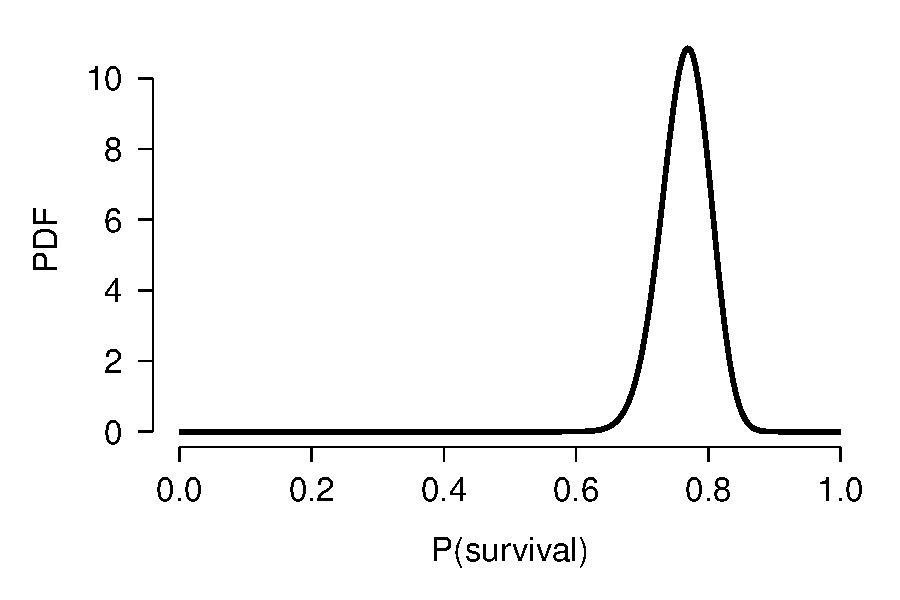
\includegraphics[keepaspectratio]{chapters/ch09_files/figure-pdf/unnamed-chunk-67-1.pdf}}
\end{center}

\subsection{Exponential distribution}\label{sec-dist-exp}

The \textbf{exponential distribution} describes the distribution of
waiting times until a single event occurs, given a constant rate per
unit time of that event occurring. This makes it the continuous analog
of the \href{@sec-dist-geom}{geometric distribution}. The exponential
distribution is also a special case of the \href{@sec-dist-gamma}{gamma
distribution} where shape parameter \(k=1\).

The exponential distribution should not be confused with the
\textbf{exponential family of distributions}, although the exponential
distribution is a member of that family. The exponential family of
distributions is a broad class that includes the normal, exponential,
gamma, beta, Poisson, and many others.

The exponential distribution is parameterized by a single rate
parameter, \(\lambda\), which describes the expected event rate per unit
time. For example, \(\lambda=2\) per day means an average waiting time
of \(1/0.2=5\) days. It does not mean exactly 0.2 events occur every
day--this is a long run average. This property means that \(\lambda\)
must be strictly positive. This is exactly the same as the rate
parameter \emph{r} sometimes used to describe the gamma distribution.
The mean of an exponential distribution \emph{X} is:

\[\mu\left(X\right)=\frac{1}{\lambda}\]

and the variance is:

\[\sigma^2\left(X\right)=\frac{1}{\lambda^2}\]

Interestingly, this implies that the standard deviation \(\sigma\) is
the same as the mean \(\mu\). Contrast this with the Poisson
distribution, where the \emph{variance} \(\sigma^2\) is the same as the
mean. Thus, the CV of the exponential distribution is always 1.

The exponential distribution is supported for all non-negative real
numbers; i.e., the half-open interval {[}0, \(+\infty\)). Like the gamma
distribution, the exponential distribution can be used when its
mechanistic assumptions make sense, such as waiting times or lifespans
with a constant event rate. It also produces strongly right-skewed
values, with many small and few large values, but right skew alone is
not sufficient reason to assume an exponential distribution.

One other important property of the exponential distribution is that it
is \emph{memoryless}. If the event rate is constant, then the
probability of waiting an additional amount of time does not depend on
how long you have already waited. For example, if mortality follows an
exponential distribution with a constant hazard, an individual that has
already survived 5 years has the same expected remaining lifespan as a
newly observed individual. The memoryless property is related to why the
\textbf{gambler's fallacy} is a fallacy. If independent events occur
with constant probability or rate, a long period without an event does
not make that event ``due.'' The geometric distribution has this
property in discrete time, and the exponential distribution has the
analogous property in continuous time.

\subsubsection{Exponential distribution in R}\label{sec-dist-exp-r}

The exponential distribution is accessed using the \texttt{\_exp} group
of functions, where the space could be \texttt{d}, \texttt{p},
\texttt{q}, or \texttt{r}. These functions calculate or returns
something different:

\begin{itemize}
\tightlist
\item
  \texttt{dexp()}: Calculates probability density function (PDF) at
  \(x\).
\item
  \texttt{pexp()}: Calculates the cumulative probability
  \(P\left(X\leq{x}\right)\). I.e., it tell you what proportion of the
  distribution lies at or below a specified value. The reverse of
  \texttt{qexp()}.
\item
  \texttt{qexp()}: Calculates the value at a specified quantile or
  quantiles. The reverse of \texttt{pexp()}.
\item
  \texttt{rexp()}: Draws random numbers from the exponential
  distribution.
\end{itemize}

\subsection{Triangular distribution}\label{sec-dist-tri}

The \textbf{triangular distribution} is sometimes used as a simple
``lack of knowledge'' distribution when little information is available
beyond a plausible minimum, maximum, and most likely value. It is used
more often to represent uncertainty in simulations and risk models than
to model observed biological data directly.

Sometimes we need to model a process about which we have very little
information. For example, we may want to simulate population dynamics
without knowing a key survival rate, or organismal growth without
knowing a key growth constant. In these situations we might have only a
vague idea of how a parameter or an outcome are distributed. At a
minimum, we can usually infer or estimate the range and central tendency
of a variable. Those are enough to estimate a triangular distribution.

The triangular distribution has three parameters: the lower limit \(a\),
the upper limit \(b\), and the mode (most common value) \(c\). Any
triangular distribution must satisfy \(a<b\) and \(a\le{c}\le{b}\).

The mean of a triangular distribution \emph{X} is the mean of its
parameters:

\[\mu\left(X\right)=\frac{a+b+c}{3}\]

and the variance is

\[\sigma^2\left(X\right)=\frac{a^2+b^2+c^2-ab-ac-bc}{18}\]

In addition to serving as a stand-in distribution when data are scarce,
the triangular distribution can arise in several natural situations. For
example, the mean of two standard uniform variables follows a triangular
distribution (see below).

\subsubsection{Triangular distribution in R}\label{sec-dist-tri-r}

The triangular distribution is available in the add-on package
\texttt{extraDistr} (Wolodzko 2026). The triangular distribution is
accessed using the \texttt{\_triang} group of functions, where the space
could be \texttt{d}, \texttt{p}, \texttt{q}, or \texttt{r}. These
functions calculate or returns something different:

\begin{itemize}
\tightlist
\item
  \texttt{dtriang()}: Calculates probability density function (PDF) at
  \(x\).
\item
  \texttt{ptriang()}: Calculates \(P\left(X\le{x}\right)\), the CDF from
  \(a\) to \(x\). The reverse of \texttt{qtriang()}.
\item
  \texttt{qtriang()}: Calculates the value at a specified quantile or
  quantiles. The reverse of \texttt{ptriang()}.
\item
  \texttt{rtriang()}: Draws random numbers from the triangular
  distribution.
\end{itemize}

The code below shows the PDFs of various triangular distributions.
Notice that \texttt{c} is not used as a variable name, to avoid
potentially masking the very critical R function \texttt{c}.

\begin{Shaded}
\begin{Highlighting}[]
\FunctionTok{library}\NormalTok{(extraDistr)}
\NormalTok{ax }\OtherTok{\textless{}{-}} \FunctionTok{c}\NormalTok{(}\DecValTok{1}\NormalTok{,}\DecValTok{1}\NormalTok{,}\DecValTok{3}\NormalTok{)}
\NormalTok{bx }\OtherTok{\textless{}{-}} \FunctionTok{c}\NormalTok{(}\DecValTok{5}\NormalTok{, }\DecValTok{10}\NormalTok{, }\DecValTok{7}\NormalTok{)}
\NormalTok{cx }\OtherTok{\textless{}{-}} \FunctionTok{c}\NormalTok{(}\DecValTok{3}\NormalTok{, }\DecValTok{3}\NormalTok{, }\DecValTok{6}\NormalTok{)}

\NormalTok{x1 }\OtherTok{\textless{}{-}} \FunctionTok{seq}\NormalTok{(ax[}\DecValTok{1}\NormalTok{], bx[}\DecValTok{1}\NormalTok{], }\AttributeTok{length=}\DecValTok{50}\NormalTok{)}
\NormalTok{x2 }\OtherTok{\textless{}{-}} \FunctionTok{seq}\NormalTok{(ax[}\DecValTok{2}\NormalTok{], bx[}\DecValTok{2}\NormalTok{], }\AttributeTok{length=}\DecValTok{50}\NormalTok{)}
\NormalTok{x3 }\OtherTok{\textless{}{-}} \FunctionTok{seq}\NormalTok{(ax[}\DecValTok{3}\NormalTok{], bx[}\DecValTok{3}\NormalTok{], }\AttributeTok{length=}\DecValTok{50}\NormalTok{)}
\NormalTok{y1 }\OtherTok{\textless{}{-}} \FunctionTok{dtriang}\NormalTok{(x1, ax[}\DecValTok{1}\NormalTok{], bx[}\DecValTok{1}\NormalTok{], cx[}\DecValTok{1}\NormalTok{])}
\NormalTok{y2 }\OtherTok{\textless{}{-}} \FunctionTok{dtriang}\NormalTok{(x2, ax[}\DecValTok{2}\NormalTok{], bx[}\DecValTok{2}\NormalTok{], cx[}\DecValTok{2}\NormalTok{])}
\NormalTok{y3 }\OtherTok{\textless{}{-}} \FunctionTok{dtriang}\NormalTok{(x3, ax[}\DecValTok{3}\NormalTok{], bx[}\DecValTok{3}\NormalTok{], cx[}\DecValTok{3}\NormalTok{])}

\FunctionTok{plot}\NormalTok{(x1, y1, }\AttributeTok{type=}\StringTok{"l"}\NormalTok{, }\AttributeTok{lwd=}\DecValTok{3}\NormalTok{, }\AttributeTok{xlab=}\StringTok{"X"}\NormalTok{, }\AttributeTok{ylab=}\StringTok{"PDF"}\NormalTok{,}
     \AttributeTok{xlim=}\FunctionTok{c}\NormalTok{(}\DecValTok{0}\NormalTok{, }\DecValTok{10}\NormalTok{))}
\FunctionTok{points}\NormalTok{(x2, y2, }\AttributeTok{type=}\StringTok{"l"}\NormalTok{, }\AttributeTok{lwd=}\DecValTok{3}\NormalTok{, }\AttributeTok{col=}\StringTok{"red"}\NormalTok{)}
\FunctionTok{points}\NormalTok{(x3, y3, }\AttributeTok{type=}\StringTok{"l"}\NormalTok{, }\AttributeTok{lwd=}\DecValTok{3}\NormalTok{, }\AttributeTok{col=}\StringTok{"blue"}\NormalTok{)}
\FunctionTok{legend}\NormalTok{(}\StringTok{"topright"}\NormalTok{, }\AttributeTok{legend=}\FunctionTok{c}\NormalTok{(}\StringTok{"Tri(1, 5, 3)"}\NormalTok{, }\StringTok{"Tri(1, 10, 3)"}\NormalTok{, }\StringTok{"Tri(3, 7, 6)"}\NormalTok{), }
       \AttributeTok{lwd=}\DecValTok{3}\NormalTok{, }\AttributeTok{col=}\FunctionTok{c}\NormalTok{(}\StringTok{"black"}\NormalTok{, }\StringTok{"red"}\NormalTok{, }\StringTok{"blue"}\NormalTok{))}
\end{Highlighting}
\end{Shaded}

\begin{center}
\pandocbounded{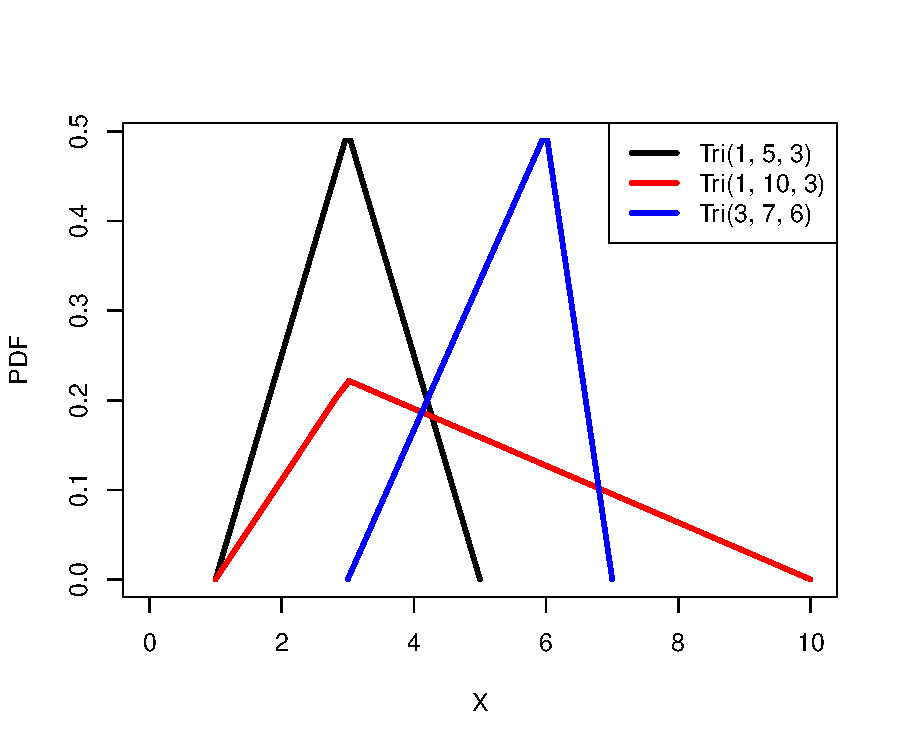
\includegraphics[keepaspectratio]{chapters/ch09_files/figure-pdf/unnamed-chunk-68-1.pdf}}
\end{center}

The code below demonstrates how a triangular distribution can arise as
the distribution of means of two standard uniform variables \texttt{x1}
and \texttt{x2}. The command \texttt{density()} calculates the kernel
density estimate of a vector. This kernel density estimate is an
empirical estimate of the PDF of a variable.

\begin{Shaded}
\begin{Highlighting}[]
\CommentTok{\# random number seed for reproducibility}
\FunctionTok{set.seed}\NormalTok{(}\DecValTok{42}\NormalTok{)}

\CommentTok{\# sample size}
\NormalTok{n }\OtherTok{\textless{}{-}} \DecValTok{10}\SpecialCharTok{\^{}}\NormalTok{(}\DecValTok{2}\SpecialCharTok{:}\DecValTok{4}\NormalTok{)}

\CommentTok{\# set up lists to hold simulation results}
\NormalTok{x1 }\OtherTok{\textless{}{-}} \FunctionTok{vector}\NormalTok{(}\StringTok{"list"}\NormalTok{, }\FunctionTok{length}\NormalTok{(n))}
\NormalTok{y }\OtherTok{\textless{}{-}} \FunctionTok{vector}\NormalTok{(}\StringTok{"list"}\NormalTok{, }\FunctionTok{length}\NormalTok{(n))}
\NormalTok{x }\OtherTok{\textless{}{-}} \FunctionTok{vector}\NormalTok{(}\StringTok{"list"}\NormalTok{, }\FunctionTok{length}\NormalTok{(n))}

\CommentTok{\# simulate uniforms in a for loop}
\ControlFlowTok{for}\NormalTok{(i }\ControlFlowTok{in} \DecValTok{1}\SpecialCharTok{:}\FunctionTok{length}\NormalTok{(n))\{}
\NormalTok{    x[[i]] }\OtherTok{\textless{}{-}}\NormalTok{ (}\FunctionTok{runif}\NormalTok{(n[i]) }\SpecialCharTok{+} \FunctionTok{runif}\NormalTok{(n[i]))}\SpecialCharTok{/}\DecValTok{2}
\NormalTok{\}}

\CommentTok{\# calculate the empirical density function}
\ControlFlowTok{for}\NormalTok{(i }\ControlFlowTok{in} \DecValTok{1}\SpecialCharTok{:}\FunctionTok{length}\NormalTok{(n))\{}
\NormalTok{    z }\OtherTok{\textless{}{-}} \FunctionTok{density}\NormalTok{(x[[i]])}
\NormalTok{    x1[[i]] }\OtherTok{\textless{}{-}}\NormalTok{ z}\SpecialCharTok{$}\NormalTok{x}
\NormalTok{    y[[i]] }\OtherTok{\textless{}{-}}\NormalTok{ z}\SpecialCharTok{$}\NormalTok{y}
\NormalTok{\}}

\CommentTok{\# make the graph}
\NormalTok{cols }\OtherTok{\textless{}{-}} \FunctionTok{rainbow}\NormalTok{(}\DecValTok{3}\NormalTok{)}
\FunctionTok{plot}\NormalTok{(x1[[}\DecValTok{1}\NormalTok{]], y[[}\DecValTok{1}\NormalTok{]], }\AttributeTok{type=}\StringTok{"l"}\NormalTok{, }\AttributeTok{lwd=}\DecValTok{3}\NormalTok{, }\AttributeTok{col=}\NormalTok{cols[}\DecValTok{1}\NormalTok{],}
     \AttributeTok{xlab=}\StringTok{"X"}\NormalTok{, }\AttributeTok{ylab=}\StringTok{"Kernel density estimate"}\NormalTok{, }\AttributeTok{ylim=}\FunctionTok{c}\NormalTok{(}\DecValTok{0}\NormalTok{, }\DecValTok{2}\NormalTok{))}
\ControlFlowTok{for}\NormalTok{(i }\ControlFlowTok{in} \DecValTok{2}\SpecialCharTok{:}\DecValTok{3}\NormalTok{)\{}
    \FunctionTok{points}\NormalTok{(x1[[i]], y[[i]], }\AttributeTok{type=}\StringTok{"l"}\NormalTok{, }\AttributeTok{lwd=}\DecValTok{3}\NormalTok{, }\AttributeTok{col=}\NormalTok{cols[i])}
\NormalTok{\}}
\FunctionTok{legend}\NormalTok{(}\StringTok{"topleft"}\NormalTok{, }\AttributeTok{legend=}\FunctionTok{c}\NormalTok{(}\StringTok{"n=100"}\NormalTok{, }\StringTok{"n=1000"}\NormalTok{, }\StringTok{"n=10000"}\NormalTok{, }\StringTok{"triangular"}\NormalTok{),}
    \AttributeTok{bty=}\StringTok{"n"}\NormalTok{, }\AttributeTok{lwd=}\DecValTok{3}\NormalTok{, }\AttributeTok{col=}\FunctionTok{c}\NormalTok{(cols[}\DecValTok{1}\SpecialCharTok{:}\DecValTok{3}\NormalTok{],}\StringTok{"black"}\NormalTok{), }\AttributeTok{lty=}\FunctionTok{c}\NormalTok{(}\DecValTok{1}\NormalTok{,}\DecValTok{1}\NormalTok{,}\DecValTok{1}\NormalTok{,}\DecValTok{2}\NormalTok{))}
\CommentTok{\# add the triangular distribution}
\FunctionTok{curve}\NormalTok{(}\FunctionTok{dtriang}\NormalTok{(x, }\DecValTok{0}\NormalTok{, }\DecValTok{1}\NormalTok{, }\FloatTok{0.5}\NormalTok{), }\AttributeTok{from=}\DecValTok{0}\NormalTok{, }\AttributeTok{to=}\DecValTok{1}\NormalTok{, }\AttributeTok{add=}\ConstantTok{TRUE}\NormalTok{, }\AttributeTok{lwd=}\DecValTok{3}\NormalTok{, }\AttributeTok{lty=}\DecValTok{2}\NormalTok{)}
\end{Highlighting}
\end{Shaded}

\begin{center}
\pandocbounded{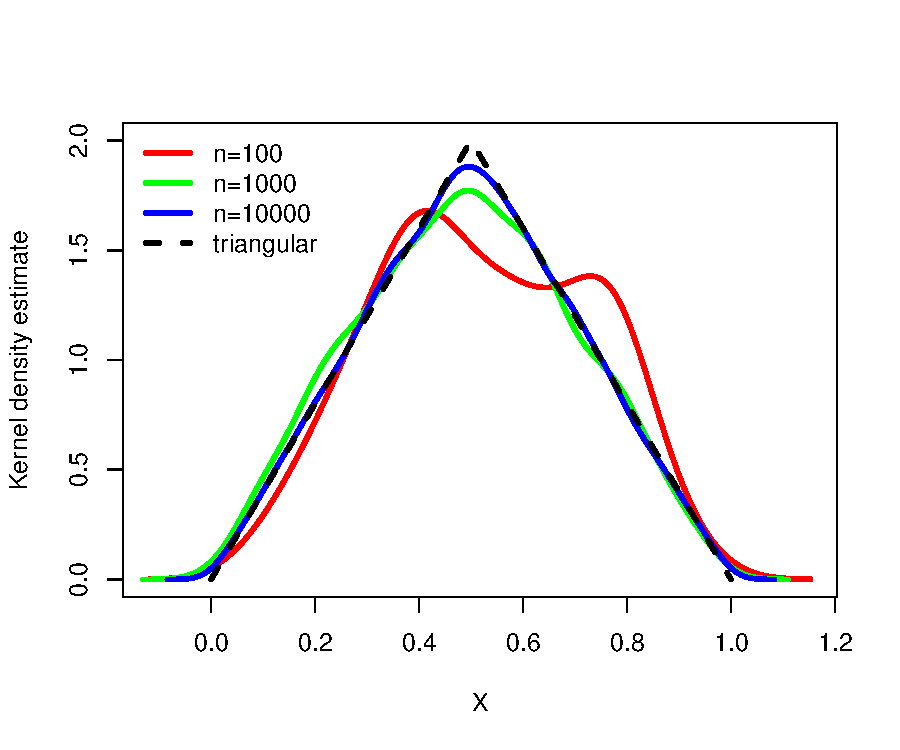
\includegraphics[keepaspectratio]{chapters/ch09_files/figure-pdf/unnamed-chunk-69-1.pdf}}
\end{center}

\subsection{Distribution summary}\label{sec-dist-summary}

The table below summarizes some the key features of the \textbf{discrete
distributions} we explored in this module.

{\def\LTcaptype{none} % do not increment counter
\begin{longtable}[]{@{}
  >{\raggedright\arraybackslash}p{(\linewidth - 4\tabcolsep) * \real{0.1105}}
  >{\raggedright\arraybackslash}p{(\linewidth - 4\tabcolsep) * \real{0.3488}}
  >{\raggedright\arraybackslash}p{(\linewidth - 4\tabcolsep) * \real{0.5407}}@{}}
\toprule\noalign{}
\begin{minipage}[b]{\linewidth}\raggedright
Distribution
\end{minipage} & \begin{minipage}[b]{\linewidth}\raggedright
Support
\end{minipage} & \begin{minipage}[b]{\linewidth}\raggedright
What it models
\end{minipage} \\
\midrule\noalign{}
\endhead
\bottomrule\noalign{}
\endlastfoot
Bernoulli & \(x\in\{0,1\}\) & Outcome of a single binary trial \\
Binomial & \(x\in\{0,1,\ldots,n\}\) & Number of successes in \(n\)
independent trials with constant probability \(p\) \\
Poisson & \(x\in\{0,1,2,\ldots\}\) & Number of events occurring
independently at a constant rate \\
Negative binomial & \(x\in\{0,1,2,\ldots\}\) & Number of failures before
a specified number of successes; commonly used for overdispersed count
data \\
Geometric & \(x\in\{0,1,2,\ldots\}\) & Number of failures before the
first success, with constant probability \(p\) \\
Beta-binomial & \(x\in\{0,1,\ldots,n\}\) & Number of successes in \(n\)
trials when the probability \(p\) varies \\
Multinomial & \(x_i\in\{0,1,\ldots,n\}\), with \(\sum_i x_i=n\) & Counts
among \(k\) categories from \(n\) trials \\
\end{longtable}
}

The table below summarizes some the key features of the
\textbf{continuous distributions} we explored in this module.

{\def\LTcaptype{none} % do not increment counter
\begin{longtable}[]{@{}
  >{\raggedright\arraybackslash}p{(\linewidth - 4\tabcolsep) * \real{0.3590}}
  >{\raggedright\arraybackslash}p{(\linewidth - 4\tabcolsep) * \real{0.2308}}
  >{\raggedright\arraybackslash}p{(\linewidth - 4\tabcolsep) * \real{0.4103}}@{}}
\toprule\noalign{}
\begin{minipage}[b]{\linewidth}\raggedright
Distribution
\end{minipage} & \begin{minipage}[b]{\linewidth}\raggedright
Support
\end{minipage} & \begin{minipage}[b]{\linewidth}\raggedright
What it models
\end{minipage} \\
\midrule\noalign{}
\endhead
\bottomrule\noalign{}
\endlastfoot
Uniform & \(x\in[a,b]\) & Continuous variables where all values within a
bounded interval are equally likely \\
Normal & \(x\in(-\infty,+\infty)\) & Continuous variables arising from
many additive processes; symmetric data concentrated around a mean \\
Lognormal & \(x\in(0,+\infty)\) & Positive variables that are normally
distributed on a log scale; often arise from multiplicative processes \\
Gamma & \(x\in(0,+\infty)\) & Positive, right-skewed variables; waiting
times until a specified number of events occurring at a constant rate \\
Beta & \(x\in[0,1]\) & Continuous proportions and probabilities,
including uncertainty about the probability of a binary event \\
Exponential & \(x\in[0,+\infty)\) & Waiting times until the first event
when events occur at a constant rate \\
Triangular & \(x\in[a,b]\) & Bounded continuous variables when only the
minimum, maximum, and most likely value are known \\
\end{longtable}
}

\begin{center}\rule{0.5\linewidth}{0.5pt}\end{center}

\chapter{Comparing data to distributions}\label{sec-dtest}

\section{Fitting and testing distributions}\label{sec-dtest-fit}

Deciding what probability distribution to use to analyze your data is an
important step in biological data analysis. The next step is to see how
well your data actually match a distribution. This section demonstrates
ways to compare data to probability distributions. We will also explore
some methods to explicitly test whether or not a set of values came from
a particular distribution.

\section{Estimating distributional
parameters}\label{sec-dtest-fit-param}

The function \texttt{fitdistr()} in package \texttt{MASS} estimates the
\textbf{parameters} of a distribution most likely to produce random
variables supplied as input. Simply put, if you have a variable
\texttt{x} and want to know what parameters of some distribution are
most likely to produce \texttt{x}, then \texttt{fitdistr()} will
estimate this for you.

\begin{Shaded}
\begin{Highlighting}[]
\FunctionTok{library}\NormalTok{(MASS)}

\FunctionTok{set.seed}\NormalTok{(}\DecValTok{123}\NormalTok{)}
\NormalTok{n }\OtherTok{\textless{}{-}} \DecValTok{50}

\CommentTok{\# estimate parameters of a normal}
\NormalTok{x1 }\OtherTok{\textless{}{-}} \FunctionTok{rnorm}\NormalTok{(n, }\DecValTok{12}\NormalTok{, }\DecValTok{2}\NormalTok{)}
\FunctionTok{fitdistr}\NormalTok{(x1, }\StringTok{"normal"}\NormalTok{)}
\end{Highlighting}
\end{Shaded}

\begin{verbatim}
      mean          sd    
  12.0688071    1.8331290 
 ( 0.2592436) ( 0.1833129)
\end{verbatim}

\begin{Shaded}
\begin{Highlighting}[]
\CommentTok{\# estimate parameters of a poisson}
\NormalTok{x2 }\OtherTok{\textless{}{-}} \FunctionTok{rpois}\NormalTok{(n, }\DecValTok{8}\NormalTok{)}
\FunctionTok{fitdistr}\NormalTok{(x2, }\StringTok{"Poisson"}\NormalTok{)}
\end{Highlighting}
\end{Shaded}

\begin{verbatim}
    lambda  
  8.2200000 
 (0.4054627)
\end{verbatim}

\begin{Shaded}
\begin{Highlighting}[]
\CommentTok{\# estimate parameters of a geometric}
\NormalTok{x3 }\OtherTok{\textless{}{-}} \FunctionTok{rgeom}\NormalTok{(n, }\FloatTok{0.7}\NormalTok{)}
\FunctionTok{fitdistr}\NormalTok{(x3, }\StringTok{"geometric"}\NormalTok{)}
\end{Highlighting}
\end{Shaded}

\begin{verbatim}
      prob   
  0.90909091 
 (0.03876377)
\end{verbatim}

\begin{Shaded}
\begin{Highlighting}[]
\CommentTok{\# estimate parameters of a beta}
\CommentTok{\# unlike most distributions, need to }
\CommentTok{\# supply starting values}
\NormalTok{x4 }\OtherTok{\textless{}{-}} \FunctionTok{rbeta}\NormalTok{(n, }\DecValTok{2}\NormalTok{, }\FloatTok{0.5}\NormalTok{)}
\FunctionTok{fitdistr}\NormalTok{(x4, }\StringTok{"beta"}\NormalTok{, }\AttributeTok{start=}\FunctionTok{list}\NormalTok{(}\AttributeTok{shape1=}\DecValTok{1}\NormalTok{, }\AttributeTok{shape2=}\DecValTok{1}\NormalTok{))}
\end{Highlighting}
\end{Shaded}

\begin{verbatim}
    shape1      shape2  
  2.1520168   0.5070293 
 (0.4828815) (0.0844015)
\end{verbatim}

\begin{Shaded}
\begin{Highlighting}[]
\CommentTok{\# estimate parameters of a negative binomial}
\NormalTok{x5 }\OtherTok{\textless{}{-}} \FunctionTok{rnbinom}\NormalTok{(n, }\DecValTok{4}\NormalTok{, }\FloatTok{0.2}\NormalTok{)}
\FunctionTok{fitdistr}\NormalTok{(x5, }\StringTok{"negative binomial"}\NormalTok{)}
\end{Highlighting}
\end{Shaded}

\begin{verbatim}
     size         mu    
   3.674590   15.660000 
 ( 0.907684) ( 1.283731)
\end{verbatim}

How did \texttt{fitdistr()} do? Most of the parameter estimates were
pretty close to the true values. The estimates generally get closer as
the sample size increases. Try increasing \texttt{n} to 500 and
rerunning the code above.

\section{Graphical methods for examining
distributions}\label{sec-dtest-fit-graph}

\subsection{Comparing distributions with PDF or PMF
plots}\label{sec-dtest-fit-pdf}

We can compare the distributions implied by the estimated parameters to
the actual data using the quantile or distribution functions. The basic
idea is to plot the data distribution, and superimpose the equivalent
plots of the hypothetical distributions.

In the example below, we compare the probability mass function (PMF) of
a discrete distribution (e.g., counts) to the PMFs of two possible
distributions that might match the data. Note that the PMF of a discrete
distribution can be estimated as the proportion of observations that
take on each value.

\begin{Shaded}
\begin{Highlighting}[]
\FunctionTok{set.seed}\NormalTok{(}\DecValTok{123}\NormalTok{)}

\CommentTok{\# the counts:}
\NormalTok{x }\OtherTok{\textless{}{-}} \FunctionTok{rnbinom}\NormalTok{(}\DecValTok{100}\NormalTok{, }\AttributeTok{mu=}\DecValTok{4}\NormalTok{, }\AttributeTok{size=}\DecValTok{2}\NormalTok{)}

\CommentTok{\# fit parameters for poisson and negative binomial}
\NormalTok{f1 }\OtherTok{\textless{}{-}} \FunctionTok{fitdistr}\NormalTok{(x, }\StringTok{"Poisson"}\NormalTok{)}
\NormalTok{f2 }\OtherTok{\textless{}{-}} \FunctionTok{fitdistr}\NormalTok{(x, }\StringTok{"negative binomial"}\NormalTok{)}

\CommentTok{\# calculate PMFs of candidate distributions across}
\CommentTok{\# range of data}
\NormalTok{xx }\OtherTok{\textless{}{-}} \DecValTok{0}\SpecialCharTok{:}\FunctionTok{max}\NormalTok{(x)}
\NormalTok{y1 }\OtherTok{\textless{}{-}} \FunctionTok{dpois}\NormalTok{(xx, f1}\SpecialCharTok{$}\NormalTok{estimate)}
\NormalTok{y2 }\OtherTok{\textless{}{-}} \FunctionTok{dnbinom}\NormalTok{(xx, }\AttributeTok{size=}\NormalTok{f2}\SpecialCharTok{$}\NormalTok{estimate[}\StringTok{"size"}\NormalTok{],}
              \AttributeTok{mu=}\NormalTok{f2}\SpecialCharTok{$}\NormalTok{estimate[}\StringTok{"mu"}\NormalTok{])}

\CommentTok{\# empirical PMF of counts}
\NormalTok{y3 }\OtherTok{\textless{}{-}} \FunctionTok{table}\NormalTok{(x)}\SpecialCharTok{/}\FunctionTok{length}\NormalTok{(x)}
\NormalTok{plot.x }\OtherTok{\textless{}{-}} \FunctionTok{as.numeric}\NormalTok{(}\FunctionTok{names}\NormalTok{(y3))}
\NormalTok{plot.y }\OtherTok{\textless{}{-}} \FunctionTok{as.numeric}\NormalTok{(y3)}

\CommentTok{\# make plot}
\FunctionTok{par}\NormalTok{(}\AttributeTok{mfrow=}\FunctionTok{c}\NormalTok{(}\DecValTok{1}\NormalTok{,}\DecValTok{1}\NormalTok{), }\AttributeTok{mar=}\FunctionTok{c}\NormalTok{(}\FloatTok{5.1}\NormalTok{, }\FloatTok{5.1}\NormalTok{, }\FloatTok{1.1}\NormalTok{, }\FloatTok{1.1}\NormalTok{),}
    \AttributeTok{las=}\DecValTok{1}\NormalTok{, }\AttributeTok{lend=}\DecValTok{1}\NormalTok{, }
    \AttributeTok{cex.axis=}\FloatTok{1.2}\NormalTok{, }\AttributeTok{cex.lab=}\FloatTok{1.2}\NormalTok{, }\AttributeTok{bty=}\StringTok{"n"}\NormalTok{)}
\FunctionTok{plot}\NormalTok{(plot.x, plot.y, }\AttributeTok{type=}\StringTok{"o"}\NormalTok{, }
    \AttributeTok{pch=}\DecValTok{15}\NormalTok{, }\AttributeTok{cex=}\FloatTok{1.3}\NormalTok{, }\AttributeTok{ylim=}\FunctionTok{c}\NormalTok{(}\DecValTok{0}\NormalTok{, }\FloatTok{0.2}\NormalTok{),}
    \AttributeTok{ylab=}\StringTok{"PMF"}\NormalTok{, }\AttributeTok{xlab=}\StringTok{"X"}\NormalTok{)}
\FunctionTok{points}\NormalTok{(xx, y1, }\AttributeTok{type=}\StringTok{"o"}\NormalTok{, }\AttributeTok{pch=}\DecValTok{16}\NormalTok{, }\AttributeTok{cex=}\FloatTok{1.3}\NormalTok{, }\AttributeTok{col=}\StringTok{"red"}\NormalTok{)}
\FunctionTok{points}\NormalTok{(xx, y2, }\AttributeTok{type=}\StringTok{"o"}\NormalTok{, }\AttributeTok{pch=}\DecValTok{17}\NormalTok{, }\AttributeTok{cex=}\FloatTok{1.3}\NormalTok{, }\AttributeTok{col=}\StringTok{"blue"}\NormalTok{)}
\FunctionTok{legend}\NormalTok{(}\StringTok{"topright"}\NormalTok{, }\AttributeTok{legend=}\FunctionTok{c}\NormalTok{(}\StringTok{"data"}\NormalTok{, }\StringTok{"Poisson"}\NormalTok{, }\StringTok{"negative binomial"}\NormalTok{),}
       \AttributeTok{pch=}\DecValTok{15}\SpecialCharTok{:}\DecValTok{17}\NormalTok{, }\AttributeTok{pt.cex=}\FloatTok{1.3}\NormalTok{,}
       \AttributeTok{col=}\FunctionTok{c}\NormalTok{(}\StringTok{"black"}\NormalTok{, }\StringTok{"red"}\NormalTok{, }\StringTok{"blue"}\NormalTok{), }\AttributeTok{bty=}\StringTok{"n"}\NormalTok{)}
\end{Highlighting}
\end{Shaded}

\begin{center}
\pandocbounded{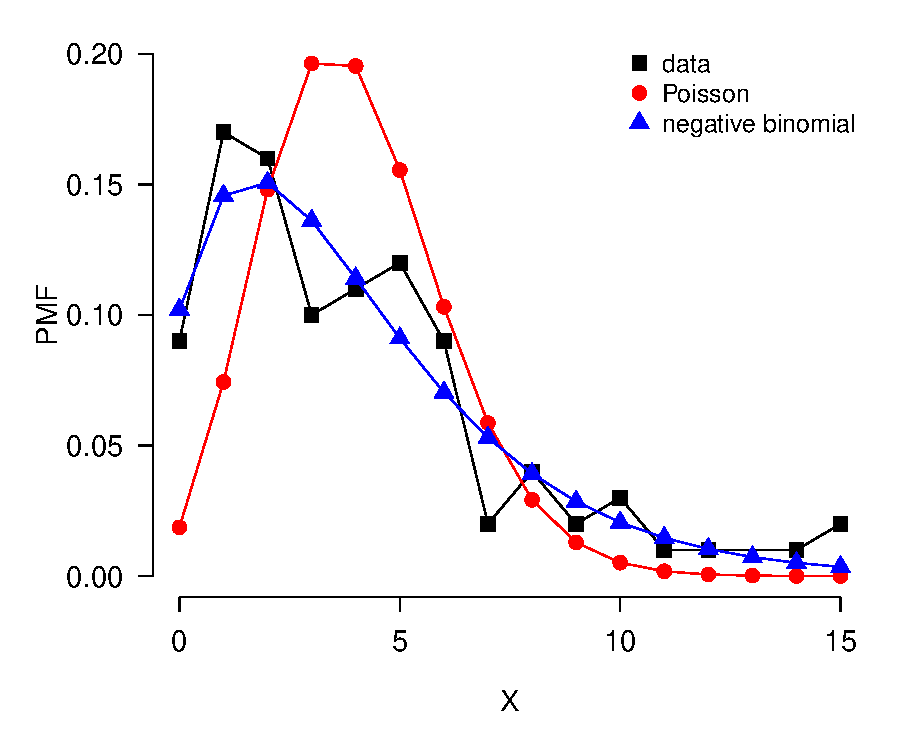
\includegraphics[keepaspectratio]{chapters/ch10_files/figure-pdf/unnamed-chunk-6-1.pdf}}
\end{center}

In this example, the data (black) seem to be better described by the
negative binomial (blue) than by the Poisson (red).

The same idea can be applied to continuous distributions. The only
difference is in how the probability density function (PDF) of the data
is estimated (note PDF, not PMF). The PDF of a continuous distribution
is estimated with function \texttt{density()}. It is a good idea to
limit the estimation of density functions to the domain of the data.
Keep in mind, however, that different distributions have different
limits. If the data contain values outside the supported interval of the
suspected distribution, that distribution cannot be correct.

The example below illustrates this: the data (\texttt{x}) are all
positive, but one of the distributions tested (normal) will produce
negative values using the estimated parameters (\texttt{f1}). That alone
should lead the researcher in this situation to eliminate the normal as
a possibility; the plot only confirms the unsuitability of the normal
for modeling \texttt{x}.

\begin{Shaded}
\begin{Highlighting}[]
\FunctionTok{set.seed}\NormalTok{(}\DecValTok{123}\NormalTok{)}

\CommentTok{\# the data:}
\NormalTok{x }\OtherTok{\textless{}{-}} \FunctionTok{rgamma}\NormalTok{(}\DecValTok{200}\NormalTok{, }\AttributeTok{shape=}\DecValTok{2}\NormalTok{, }\AttributeTok{scale=}\DecValTok{20}\NormalTok{)}
\FunctionTok{hist}\NormalTok{(x)}
\end{Highlighting}
\end{Shaded}

\begin{center}
\pandocbounded{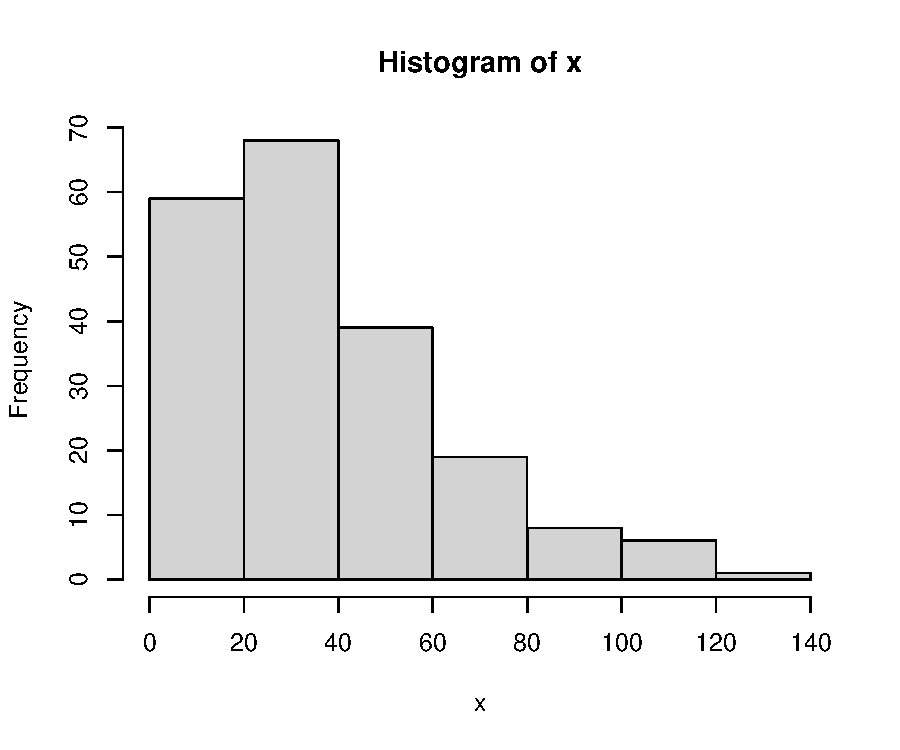
\includegraphics[keepaspectratio]{chapters/ch10_files/figure-pdf/unnamed-chunk-7-1.pdf}}
\end{center}

\begin{Shaded}
\begin{Highlighting}[]
\CommentTok{\# fit parameters for poisson and negative binomial}
\NormalTok{f1 }\OtherTok{\textless{}{-}} \FunctionTok{fitdistr}\NormalTok{(x, }\StringTok{"normal"}\NormalTok{)}
\NormalTok{f2 }\OtherTok{\textless{}{-}} \FunctionTok{fitdistr}\NormalTok{(x, }\StringTok{"lognormal"}\NormalTok{)}
\NormalTok{f3 }\OtherTok{\textless{}{-}} \FunctionTok{fitdistr}\NormalTok{(x, }\StringTok{"gamma"}\NormalTok{)}

\CommentTok{\# calculate PMFs of candidate distributions across}
\CommentTok{\# range of data}
\NormalTok{xx }\OtherTok{\textless{}{-}} \FunctionTok{seq}\NormalTok{(}\FunctionTok{min}\NormalTok{(x), }\FunctionTok{max}\NormalTok{(x), }\AttributeTok{length=}\DecValTok{1000}\NormalTok{)}
\NormalTok{y1 }\OtherTok{\textless{}{-}} \FunctionTok{dnorm}\NormalTok{(xx, f1}\SpecialCharTok{$}\NormalTok{estimate[}\DecValTok{1}\NormalTok{], f1}\SpecialCharTok{$}\NormalTok{estimate[}\DecValTok{2}\NormalTok{])}
\NormalTok{y2 }\OtherTok{\textless{}{-}} \FunctionTok{dlnorm}\NormalTok{(xx, f2}\SpecialCharTok{$}\NormalTok{estimate[}\DecValTok{1}\NormalTok{], f2}\SpecialCharTok{$}\NormalTok{estimate[}\DecValTok{2}\NormalTok{])}
\NormalTok{y3 }\OtherTok{\textless{}{-}} \FunctionTok{dgamma}\NormalTok{(xx, }\AttributeTok{shape=}\NormalTok{f3}\SpecialCharTok{$}\NormalTok{estimate[}\DecValTok{1}\NormalTok{], }\AttributeTok{rate=}\NormalTok{f3}\SpecialCharTok{$}\NormalTok{estimate[}\DecValTok{2}\NormalTok{])}

\CommentTok{\# empirical PDF of data}
\NormalTok{dx }\OtherTok{\textless{}{-}} \FunctionTok{density}\NormalTok{(x, }\AttributeTok{from=}\FunctionTok{min}\NormalTok{(x), }\AttributeTok{to=}\FunctionTok{max}\NormalTok{(x))}

\CommentTok{\# make plot}
\FunctionTok{par}\NormalTok{(}\AttributeTok{mfrow=}\FunctionTok{c}\NormalTok{(}\DecValTok{1}\NormalTok{,}\DecValTok{1}\NormalTok{), }\AttributeTok{mar=}\FunctionTok{c}\NormalTok{(}\FloatTok{5.1}\NormalTok{, }\FloatTok{5.1}\NormalTok{, }\FloatTok{1.1}\NormalTok{, }\FloatTok{1.1}\NormalTok{),}
    \AttributeTok{las=}\DecValTok{1}\NormalTok{, }\AttributeTok{lend=}\DecValTok{1}\NormalTok{, }
    \AttributeTok{cex.axis=}\FloatTok{1.2}\NormalTok{, }\AttributeTok{cex.lab=}\FloatTok{1.2}\NormalTok{, }\AttributeTok{bty=}\StringTok{"n"}\NormalTok{)}
\FunctionTok{plot}\NormalTok{(dx}\SpecialCharTok{$}\NormalTok{x, dx}\SpecialCharTok{$}\NormalTok{y,}
    \AttributeTok{type=}\StringTok{"l"}\NormalTok{, }\AttributeTok{lwd=}\DecValTok{3}\NormalTok{, }\AttributeTok{ylim=}\FunctionTok{c}\NormalTok{(}\DecValTok{0}\NormalTok{, }\FloatTok{0.025}\NormalTok{),}
    \AttributeTok{ylab=}\StringTok{""}\NormalTok{, }\AttributeTok{xlab=}\StringTok{"X"}\NormalTok{)}
\FunctionTok{title}\NormalTok{(}\AttributeTok{ylab=}\StringTok{"PDF"}\NormalTok{, }\AttributeTok{line=}\DecValTok{4}\NormalTok{)}
\FunctionTok{points}\NormalTok{(xx, y1, }\AttributeTok{type=}\StringTok{"l"}\NormalTok{, }\AttributeTok{lwd=}\DecValTok{3}\NormalTok{, }\AttributeTok{col=}\StringTok{"red"}\NormalTok{)}
\FunctionTok{points}\NormalTok{(xx, y2, }\AttributeTok{type=}\StringTok{"l"}\NormalTok{, }\AttributeTok{lwd=}\DecValTok{3}\NormalTok{, }\AttributeTok{col=}\StringTok{"blue"}\NormalTok{)}
\FunctionTok{points}\NormalTok{(xx, y3, }\AttributeTok{type=}\StringTok{"l"}\NormalTok{, }\AttributeTok{lwd=}\DecValTok{3}\NormalTok{, }\AttributeTok{col=}\StringTok{"green"}\NormalTok{)}
\FunctionTok{legend}\NormalTok{(}\StringTok{"topright"}\NormalTok{, }
    \AttributeTok{legend=}\FunctionTok{c}\NormalTok{(}\StringTok{"data"}\NormalTok{, }\StringTok{"normal"}\NormalTok{, }\StringTok{"lognormal"}\NormalTok{, }\StringTok{"gamma"}\NormalTok{),}
    \AttributeTok{lwd=}\DecValTok{3}\NormalTok{, }\AttributeTok{col=}\FunctionTok{c}\NormalTok{(}\StringTok{"black"}\NormalTok{, }\StringTok{"red"}\NormalTok{, }\StringTok{"blue"}\NormalTok{, }\StringTok{"green"}\NormalTok{),}
    \AttributeTok{cex=}\FloatTok{1.3}\NormalTok{, }\AttributeTok{bty=}\StringTok{"n"}\NormalTok{)}
\end{Highlighting}
\end{Shaded}

\begin{center}
\pandocbounded{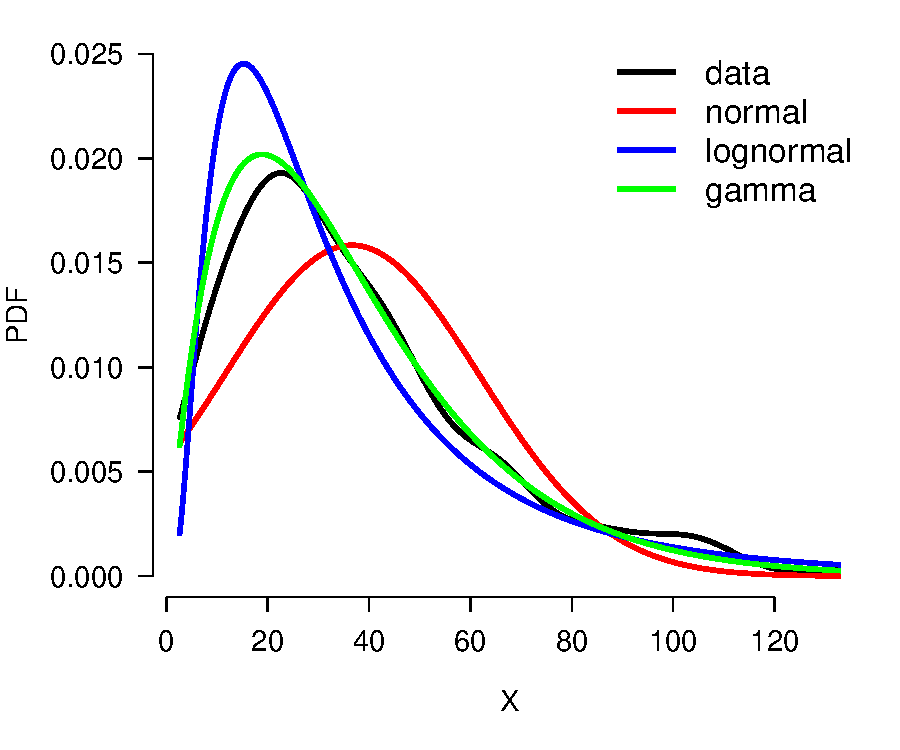
\includegraphics[keepaspectratio]{chapters/ch10_files/figure-pdf/unnamed-chunk-8-1.pdf}}
\end{center}

The plot suggests that the data are better described by a gamma
distribution than by a normal or lognormal. This is because the curve
for the data is most closely matched by the curve for the gamma. Try
adjusting the sample size in the example above (e.g.,
\texttt{n\ \textless{}-\ 50}) and see if the correct distribution always
matches the data.

\subsection{Comparing distributions using CDF and
ECDF}\label{sec-dtest-fit-cdf}

Another way to compare data to distributions is with the cumulative
distribution function (CDF). The basic idea is the same as using density
functions: compare the empirical CDF (ECDF) of the data to the CDFs
potential distributions and judge which one best matches the data.

The example below shows how to use ECDF and CDF to compare a continuous
distribution to various target distributions.

\begin{Shaded}
\begin{Highlighting}[]
\FunctionTok{set.seed}\NormalTok{(}\DecValTok{123}\NormalTok{)}

\CommentTok{\# make the data:}
\NormalTok{x }\OtherTok{\textless{}{-}} \FunctionTok{rlnorm}\NormalTok{(}\DecValTok{100}\NormalTok{, }\AttributeTok{meanlog=}\FunctionTok{log}\NormalTok{(}\DecValTok{4}\NormalTok{), }\AttributeTok{sdlog=}\FunctionTok{log}\NormalTok{(}\DecValTok{3}\NormalTok{))}

\CommentTok{\# fit some distributions}
\NormalTok{f1 }\OtherTok{\textless{}{-}} \FunctionTok{fitdistr}\NormalTok{(x, }\StringTok{"normal"}\NormalTok{)}
\NormalTok{f2 }\OtherTok{\textless{}{-}} \FunctionTok{fitdistr}\NormalTok{(x, }\StringTok{"lognormal"}\NormalTok{)}
\NormalTok{f3 }\OtherTok{\textless{}{-}} \FunctionTok{fitdistr}\NormalTok{(x, }\StringTok{"gamma"}\NormalTok{)}
\NormalTok{f4 }\OtherTok{\textless{}{-}} \FunctionTok{fitdistr}\NormalTok{(x, }\StringTok{"exponential"}\NormalTok{)}

\CommentTok{\# calculate density functions over domain of x}
\NormalTok{xx }\OtherTok{\textless{}{-}} \FunctionTok{seq}\NormalTok{(}\FunctionTok{min}\NormalTok{(x), }\FunctionTok{max}\NormalTok{(x), }\AttributeTok{length=}\DecValTok{100}\NormalTok{)}
\NormalTok{y1 }\OtherTok{\textless{}{-}} \FunctionTok{pnorm}\NormalTok{(xx, f1}\SpecialCharTok{$}\NormalTok{estimate[}\StringTok{"mean"}\NormalTok{], f1}\SpecialCharTok{$}\NormalTok{estimate[}\StringTok{"sd"}\NormalTok{])}
\NormalTok{y2 }\OtherTok{\textless{}{-}} \FunctionTok{plnorm}\NormalTok{(xx, f2}\SpecialCharTok{$}\NormalTok{estimate[}\StringTok{"meanlog"}\NormalTok{], f2}\SpecialCharTok{$}\NormalTok{estimate[}\StringTok{"sdlog"}\NormalTok{])}
\NormalTok{y3 }\OtherTok{\textless{}{-}} \FunctionTok{pgamma}\NormalTok{(xx,}
             \AttributeTok{shape=}\NormalTok{f3}\SpecialCharTok{$}\NormalTok{estimate[}\StringTok{"shape"}\NormalTok{], }
             \AttributeTok{rate=}\NormalTok{f3}\SpecialCharTok{$}\NormalTok{estimate[}\StringTok{"rate"}\NormalTok{])}
\NormalTok{y4 }\OtherTok{\textless{}{-}} \FunctionTok{pexp}\NormalTok{(xx, }\AttributeTok{rate=}\NormalTok{f4}\SpecialCharTok{$}\NormalTok{estimate[}\StringTok{"rate"}\NormalTok{])}

\CommentTok{\# ecdf of data}
\NormalTok{y5 }\OtherTok{\textless{}{-}} \FunctionTok{ecdf}\NormalTok{(x)(xx)}

\CommentTok{\# fancy plot}
\NormalTok{cols }\OtherTok{\textless{}{-}} \FunctionTok{c}\NormalTok{(}\StringTok{"black"}\NormalTok{, }\FunctionTok{rainbow}\NormalTok{(}\DecValTok{4}\NormalTok{))}
\FunctionTok{par}\NormalTok{(}\AttributeTok{mfrow=}\FunctionTok{c}\NormalTok{(}\DecValTok{1}\NormalTok{,}\DecValTok{1}\NormalTok{), }\AttributeTok{mar=}\FunctionTok{c}\NormalTok{(}\FloatTok{5.1}\NormalTok{, }\FloatTok{5.1}\NormalTok{, }\FloatTok{1.1}\NormalTok{, }\FloatTok{1.1}\NormalTok{),}
    \AttributeTok{las=}\DecValTok{1}\NormalTok{, }\AttributeTok{lend=}\DecValTok{1}\NormalTok{, }
    \AttributeTok{cex.axis=}\FloatTok{1.2}\NormalTok{, }\AttributeTok{cex.lab=}\FloatTok{1.2}\NormalTok{, }\AttributeTok{bty=}\StringTok{"n"}\NormalTok{)}
\FunctionTok{plot}\NormalTok{(xx, y5, }\AttributeTok{type=}\StringTok{"l"}\NormalTok{, }\AttributeTok{lwd=}\DecValTok{3}\NormalTok{, }\AttributeTok{xlab=}\StringTok{"X"}\NormalTok{,}
    \AttributeTok{ylab=}\StringTok{"(E)CDF"}\NormalTok{, }\AttributeTok{ylim=}\FunctionTok{c}\NormalTok{(}\DecValTok{0}\NormalTok{,}\DecValTok{1}\NormalTok{), }\AttributeTok{col=}\NormalTok{cols[}\DecValTok{1}\NormalTok{])}
\FunctionTok{points}\NormalTok{(xx, y1, }\AttributeTok{type=}\StringTok{"l"}\NormalTok{, }\AttributeTok{lwd=}\DecValTok{3}\NormalTok{, }\AttributeTok{col=}\NormalTok{cols[}\DecValTok{2}\NormalTok{])}
\FunctionTok{points}\NormalTok{(xx, y2, }\AttributeTok{type=}\StringTok{"l"}\NormalTok{, }\AttributeTok{lwd=}\DecValTok{3}\NormalTok{, }\AttributeTok{col=}\NormalTok{cols[}\DecValTok{3}\NormalTok{])}
\FunctionTok{points}\NormalTok{(xx, y3, }\AttributeTok{type=}\StringTok{"l"}\NormalTok{, }\AttributeTok{lwd=}\DecValTok{3}\NormalTok{, }\AttributeTok{col=}\NormalTok{cols[}\DecValTok{4}\NormalTok{])}
\FunctionTok{points}\NormalTok{(xx, y4, }\AttributeTok{type=}\StringTok{"l"}\NormalTok{, }\AttributeTok{lwd=}\DecValTok{3}\NormalTok{, }\AttributeTok{col=}\NormalTok{cols[}\DecValTok{5}\NormalTok{])}
\FunctionTok{legend}\NormalTok{(}\StringTok{"bottomright"}\NormalTok{, }
    \AttributeTok{legend=}\FunctionTok{c}\NormalTok{(}\StringTok{"ECDF(data)"}\NormalTok{, }\StringTok{"Normal"}\NormalTok{, }\StringTok{"Lognormal"}\NormalTok{, }\StringTok{"Gamma"}\NormalTok{, }\StringTok{"Exponential"}\NormalTok{), }
    \AttributeTok{lwd=}\DecValTok{3}\NormalTok{, }\AttributeTok{col=}\NormalTok{cols, }\AttributeTok{bty=}\StringTok{"n"}\NormalTok{, }\AttributeTok{cex=}\FloatTok{1.3}\NormalTok{)}
\end{Highlighting}
\end{Shaded}

\begin{center}
\pandocbounded{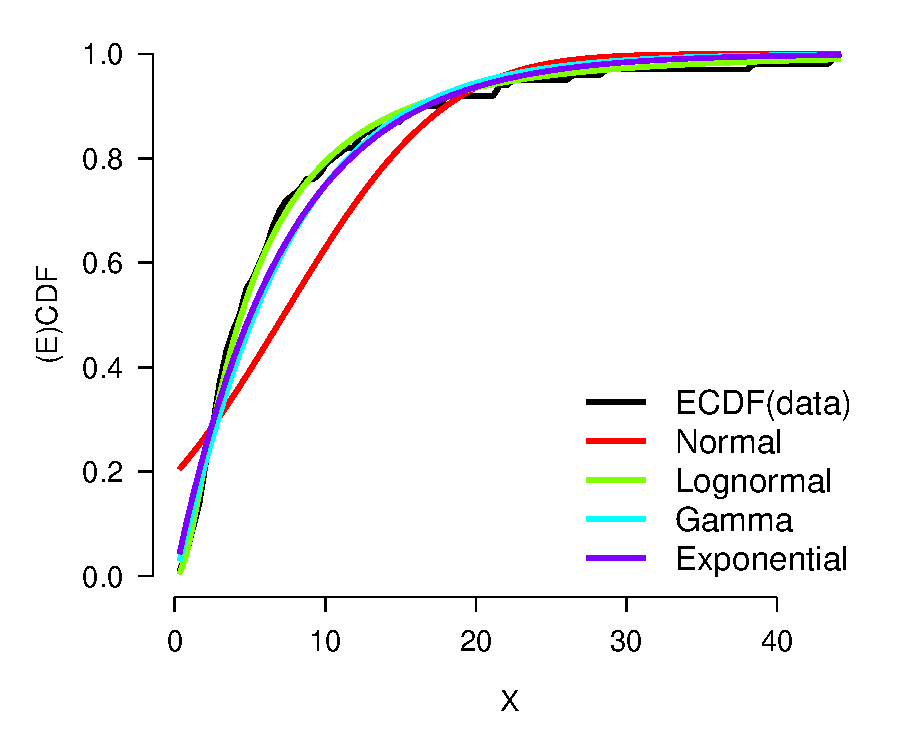
\includegraphics[keepaspectratio]{chapters/ch10_files/figure-pdf/unnamed-chunk-9-1.pdf}}
\end{center}

In this example, the ECDF of the original data (black) appears to best
match the lognormal (green)---as well it should, because the data came
from a lognormal distribution. The normal (red) is clearly inappropriate
because it diverges from the actual data over most of the range of the
data. The gamma and exponential are each better than the normal, but not
as close to the data as the lognormal.

\subsection{Comparing distributions using QQ
plots}\label{sec-dtest-fit-qq}

Finally, you can use \textbf{quantile-quantile (QQ) plots} to compare
data to different distributions that you suspect they may follow. The
example below uses a QQ plot instead of ECDF as seen above.

\begin{Shaded}
\begin{Highlighting}[]
\FunctionTok{set.seed}\NormalTok{(}\DecValTok{123}\NormalTok{)}

\CommentTok{\# true distribution: lognormal}
\NormalTok{n }\OtherTok{\textless{}{-}} \DecValTok{100}
\NormalTok{x }\OtherTok{\textless{}{-}} \FunctionTok{rlnorm}\NormalTok{(n, }\AttributeTok{meanlog=}\FunctionTok{log}\NormalTok{(}\DecValTok{4}\NormalTok{), }\AttributeTok{sdlog=}\FunctionTok{log}\NormalTok{(}\DecValTok{3}\NormalTok{))}

\CommentTok{\# estimate distributional parameters}
\NormalTok{f1 }\OtherTok{\textless{}{-}} \FunctionTok{fitdistr}\NormalTok{(x, }\StringTok{"normal"}\NormalTok{)}
\NormalTok{f2 }\OtherTok{\textless{}{-}} \FunctionTok{fitdistr}\NormalTok{(x, }\StringTok{"lognormal"}\NormalTok{)}
\NormalTok{f3 }\OtherTok{\textless{}{-}} \FunctionTok{fitdistr}\NormalTok{(x, }\StringTok{"gamma"}\NormalTok{)}
\NormalTok{f4 }\OtherTok{\textless{}{-}} \FunctionTok{fitdistr}\NormalTok{(x, }\StringTok{"exponential"}\NormalTok{)}

\CommentTok{\# quantiles of reference distribution}
\NormalTok{qx }\OtherTok{\textless{}{-}} \FunctionTok{ppoints}\NormalTok{(n)}

\CommentTok{\# define functions to draw from each reference distribution}
\NormalTok{dfun1 }\OtherTok{\textless{}{-}} \ControlFlowTok{function}\NormalTok{(p)\{}\FunctionTok{qnorm}\NormalTok{(p, f1}\SpecialCharTok{$}\NormalTok{estimate[}\DecValTok{1}\NormalTok{], f1}\SpecialCharTok{$}\NormalTok{estimate[}\DecValTok{2}\NormalTok{])\}}
\NormalTok{dfun2 }\OtherTok{\textless{}{-}} \ControlFlowTok{function}\NormalTok{(p)\{}\FunctionTok{qlnorm}\NormalTok{(p, f2}\SpecialCharTok{$}\NormalTok{estimate[}\DecValTok{1}\NormalTok{], f2}\SpecialCharTok{$}\NormalTok{estimate[}\DecValTok{2}\NormalTok{])\}}
\NormalTok{dfun3 }\OtherTok{\textless{}{-}} \ControlFlowTok{function}\NormalTok{(p)\{}\FunctionTok{qgamma}\NormalTok{(p, }\AttributeTok{shape=}\NormalTok{f3}\SpecialCharTok{$}\NormalTok{estimate[}\DecValTok{1}\NormalTok{],}
                            \AttributeTok{rate=}\NormalTok{f3}\SpecialCharTok{$}\NormalTok{estimate[}\DecValTok{2}\NormalTok{])\}}
\NormalTok{dfun4 }\OtherTok{\textless{}{-}} \ControlFlowTok{function}\NormalTok{(p)\{}\FunctionTok{qexp}\NormalTok{(p, f4}\SpecialCharTok{$}\NormalTok{estimate)\}}

\CommentTok{\# get values at each reference quantile}
\NormalTok{qy1 }\OtherTok{\textless{}{-}} \FunctionTok{dfun1}\NormalTok{(qx)}
\NormalTok{qy2 }\OtherTok{\textless{}{-}} \FunctionTok{dfun2}\NormalTok{(qx)}
\NormalTok{qy3 }\OtherTok{\textless{}{-}} \FunctionTok{dfun3}\NormalTok{(qx)}
\NormalTok{qy4 }\OtherTok{\textless{}{-}} \FunctionTok{dfun4}\NormalTok{(qx)}

\CommentTok{\# make plot}
\FunctionTok{par}\NormalTok{(}\AttributeTok{mfrow=}\FunctionTok{c}\NormalTok{(}\DecValTok{2}\NormalTok{,}\DecValTok{2}\NormalTok{), }\AttributeTok{mar=}\FunctionTok{c}\NormalTok{(}\FloatTok{5.1}\NormalTok{, }\FloatTok{5.1}\NormalTok{, }\FloatTok{1.1}\NormalTok{, }\FloatTok{1.1}\NormalTok{),}
    \AttributeTok{las=}\DecValTok{1}\NormalTok{, }\AttributeTok{lend=}\DecValTok{1}\NormalTok{, }
    \AttributeTok{cex.axis=}\FloatTok{1.2}\NormalTok{, }\AttributeTok{cex.lab=}\FloatTok{1.2}\NormalTok{, }\AttributeTok{bty=}\StringTok{"n"}\NormalTok{)}
\FunctionTok{qqplot}\NormalTok{(qy1, x, }\AttributeTok{main=}\StringTok{"Normal"}\NormalTok{)}
\FunctionTok{qqline}\NormalTok{(x, }\AttributeTok{distribution=}\NormalTok{dfun1, }\AttributeTok{col=}\StringTok{"red"}\NormalTok{)}
\FunctionTok{qqplot}\NormalTok{(qy2, x, }\AttributeTok{main=}\StringTok{"Lognormal"}\NormalTok{)}
\FunctionTok{qqline}\NormalTok{(x, }\AttributeTok{distribution=}\NormalTok{dfun2, }\AttributeTok{col=}\StringTok{"red"}\NormalTok{)}
\FunctionTok{qqplot}\NormalTok{(qy3, x, }\AttributeTok{main=}\StringTok{"Gamma"}\NormalTok{)}
\FunctionTok{qqline}\NormalTok{(x, }\AttributeTok{distribution=}\NormalTok{dfun3, }\AttributeTok{col=}\StringTok{"red"}\NormalTok{)}
\FunctionTok{qqplot}\NormalTok{(qy4, x, }\AttributeTok{main=}\StringTok{"Exponential"}\NormalTok{)}
\FunctionTok{qqline}\NormalTok{(x, }\AttributeTok{distribution=}\NormalTok{dfun4, }\AttributeTok{col=}\StringTok{"red"}\NormalTok{)}
\end{Highlighting}
\end{Shaded}

\begin{center}
\pandocbounded{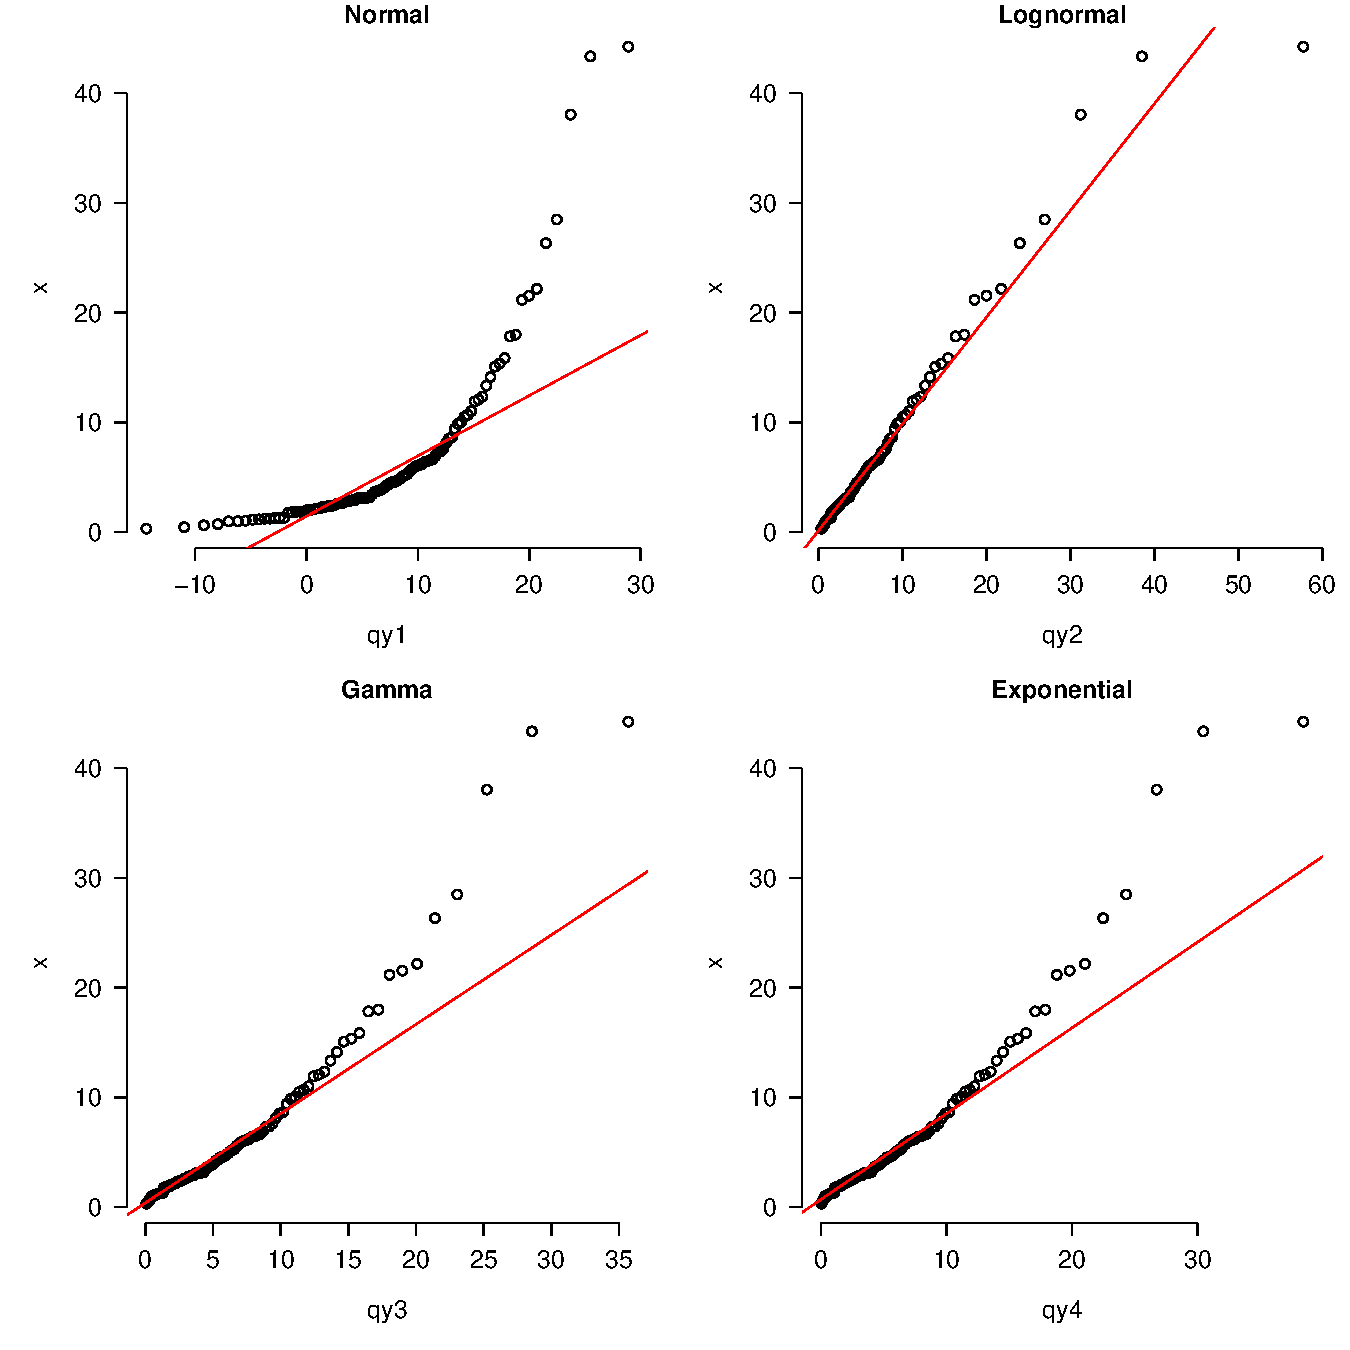
\includegraphics[keepaspectratio]{chapters/ch10_files/figure-pdf/unnamed-chunk-10-1.pdf}}
\end{center}

The figure shows that the normal is clearly inappropriate because the
points do not fall on the line. The gamma and exponential are okay over
most of the domain of x, but depart for large values. The lognormal plot
(top right) shows the best match between the data and the reference
distribution.

It is important to keep in mind that the comparisons we've made here are
of idealized cases. Real data are often much messier and noisier than
the distributions used in these examples. Sometimes real data are best
characterized by mixture distributions for which there are no
straightforward ways to estimate parameters. Still, the steps outlined
above for estimating distributional parameters and comparing to
idealized distributions are important first steps in data analysis.

\section{Formal tests for distributions}\label{sec-dtest-tests}

\subsection{Tests for normality}\label{sec-dtest-tests-norm}

The normal distribution is so important for so many statistical methods
that people have developed tests to formally determine whether data come
from a normal distribution. The most common test for normality is the
\textbf{Shapiro-Wilk test}. The Shapiro-Wilk test tests the null
hypothesis that a sample \emph{x}\textsubscript{1}, \ldots,
\emph{x\textsubscript{n}} comes from a normally distributed population.
The test statistic \emph{W} is calculated as:

\[W=\frac{\left(\sum_{i=1}^{n}{a_ix_{(i)}}\right)^2}{\sum_{i=1}^{n}\left(x_i-\bar{x}\right)^2}\]

where \(\bar{x}\) is the sample mean, \(x_i\)\textasciitilde{} is the
\(i^{th}\) order statistic, and \(a_i\) is a coefficient related to
expected values of \emph{i.i.d.} normal variables. When the null
hypothesis of a Shapiro-Wilk test is rejected, then there is evidence
that the data are not normally distributed. The code below shows some
examples of the Shapiro-Wilk test in R.

\begin{Shaded}
\begin{Highlighting}[]
\FunctionTok{set.seed}\NormalTok{(}\DecValTok{123}\NormalTok{)}
\NormalTok{x1 }\OtherTok{\textless{}{-}} \FunctionTok{rnorm}\NormalTok{(}\DecValTok{20}\NormalTok{)}
\FunctionTok{shapiro.test}\NormalTok{(x1)}
\DocumentationTok{\#\# }
\DocumentationTok{\#\#  Shapiro{-}Wilk normality test}
\DocumentationTok{\#\# }
\DocumentationTok{\#\# data:  x1}
\DocumentationTok{\#\# W = 0.96858, p{-}value = 0.7247}
\end{Highlighting}
\end{Shaded}

\begin{Shaded}
\begin{Highlighting}[]
\NormalTok{x2 }\OtherTok{\textless{}{-}} \FunctionTok{rpois}\NormalTok{(}\DecValTok{20}\NormalTok{, }\DecValTok{10}\NormalTok{)}
\FunctionTok{shapiro.test}\NormalTok{(x2)}
\end{Highlighting}
\end{Shaded}

\begin{verbatim}

    Shapiro-Wilk normality test

data:  x2
W = 0.90741, p-value = 0.0569
\end{verbatim}

\begin{Shaded}
\begin{Highlighting}[]
\NormalTok{x3 }\OtherTok{\textless{}{-}} \FunctionTok{runif}\NormalTok{(}\DecValTok{20}\NormalTok{)}
\FunctionTok{shapiro.test}\NormalTok{(x3)}
\end{Highlighting}
\end{Shaded}

\begin{verbatim}

    Shapiro-Wilk normality test

data:  x3
W = 0.9316, p-value = 0.1658
\end{verbatim}

\begin{Shaded}
\begin{Highlighting}[]
\NormalTok{x4 }\OtherTok{\textless{}{-}} \FunctionTok{runif}\NormalTok{(}\DecValTok{100}\NormalTok{)}
\FunctionTok{shapiro.test}\NormalTok{(x4)}
\end{Highlighting}
\end{Shaded}

\begin{verbatim}

    Shapiro-Wilk normality test

data:  x4
W = 0.96392, p-value = 0.007723
\end{verbatim}

Interestingly, the Shapiro-Wilk test turns out to be very powerful. That
is, it can detect very small differences from the null hypothesis (i.e.,
normality) if the sample size is large enough. So, if you have data that
you suspect are normal, but the Shapiro-Wilk test says otherwise, you
need to visually inspect the data to determine how serious the departure
from normality is.

\subsection{Kolmogorov-Smirnov tests}\label{sec-dtest-tests-ks}

The \textbf{Kolmogorov-Smirnov (KS) test} is a non-parametric test that
compares a dataset to a distribution. Unlike the Shapiro-Wilk test,
which only tests for normality, the KS test can compare data to any
distribution. The KS test is useful because it is sensitive to
differences in both location (i.e., mean) and shape. The example below
illustrates the use of the KS test and plots the distributions.

\begin{Shaded}
\begin{Highlighting}[]
\NormalTok{n }\OtherTok{\textless{}{-}} \FloatTok{1e2}
\NormalTok{x1 }\OtherTok{\textless{}{-}} \FunctionTok{rnorm}\NormalTok{(n, }\DecValTok{10}\NormalTok{, }\DecValTok{2}\NormalTok{)}
\NormalTok{x2 }\OtherTok{\textless{}{-}} \FunctionTok{rnorm}\NormalTok{(n, }\DecValTok{10}\NormalTok{, }\DecValTok{2}\NormalTok{)}
\NormalTok{x3 }\OtherTok{\textless{}{-}} \FunctionTok{rnorm}\NormalTok{(n, }\DecValTok{14}\NormalTok{, }\DecValTok{2}\NormalTok{)}
\NormalTok{x4 }\OtherTok{\textless{}{-}} \FunctionTok{rnorm}\NormalTok{(n, }\DecValTok{14}\NormalTok{, }\DecValTok{20}\NormalTok{)}
\NormalTok{x5 }\OtherTok{\textless{}{-}} \FunctionTok{rpois}\NormalTok{(n, }\DecValTok{14}\NormalTok{)}

\CommentTok{\# run KS tests:}
\FunctionTok{ks.test}\NormalTok{(x1, x2)}
\end{Highlighting}
\end{Shaded}

\begin{verbatim}

    Asymptotic two-sample Kolmogorov-Smirnov test

data:  x1 and x2
D = 0.1, p-value = 0.6994
alternative hypothesis: two-sided
\end{verbatim}

\begin{Shaded}
\begin{Highlighting}[]
\FunctionTok{ks.test}\NormalTok{(x1, x3)}
\end{Highlighting}
\end{Shaded}

\begin{verbatim}

    Asymptotic two-sample Kolmogorov-Smirnov test

data:  x1 and x3
D = 0.66, p-value < 2.2e-16
alternative hypothesis: two-sided
\end{verbatim}

\begin{Shaded}
\begin{Highlighting}[]
\FunctionTok{ks.test}\NormalTok{(x3, x4)}
\end{Highlighting}
\end{Shaded}

\begin{verbatim}

    Asymptotic two-sample Kolmogorov-Smirnov test

data:  x3 and x4
D = 0.41, p-value = 1.001e-07
alternative hypothesis: two-sided
\end{verbatim}

\begin{Shaded}
\begin{Highlighting}[]
\FunctionTok{ks.test}\NormalTok{(x3, x5)}
\end{Highlighting}
\end{Shaded}

\begin{verbatim}

    Asymptotic two-sample Kolmogorov-Smirnov test

data:  x3 and x5
D = 0.25, p-value = 0.003861
alternative hypothesis: two-sided
\end{verbatim}

\begin{Shaded}
\begin{Highlighting}[]
\CommentTok{\# make a plot}
\NormalTok{xx }\OtherTok{\textless{}{-}} \DecValTok{5}\SpecialCharTok{:}\DecValTok{25}
\NormalTok{y1 }\OtherTok{\textless{}{-}} \FunctionTok{ecdf}\NormalTok{(x1)(xx)}
\NormalTok{y2 }\OtherTok{\textless{}{-}} \FunctionTok{ecdf}\NormalTok{(x2)(xx)}
\NormalTok{y3 }\OtherTok{\textless{}{-}} \FunctionTok{ecdf}\NormalTok{(x3)(xx)}
\NormalTok{y4 }\OtherTok{\textless{}{-}} \FunctionTok{ecdf}\NormalTok{(x4)(xx)}
\NormalTok{y5 }\OtherTok{\textless{}{-}} \FunctionTok{ecdf}\NormalTok{(x5)(xx)}

\NormalTok{cols }\OtherTok{\textless{}{-}} \FunctionTok{rainbow}\NormalTok{(}\DecValTok{5}\NormalTok{)}
\FunctionTok{par}\NormalTok{(}\AttributeTok{mfrow=}\FunctionTok{c}\NormalTok{(}\DecValTok{1}\NormalTok{,}\DecValTok{1}\NormalTok{), }\AttributeTok{mar=}\FunctionTok{c}\NormalTok{(}\FloatTok{5.1}\NormalTok{, }\FloatTok{5.1}\NormalTok{, }\FloatTok{1.1}\NormalTok{, }\FloatTok{1.1}\NormalTok{),}
    \AttributeTok{bty=}\StringTok{"n"}\NormalTok{, }\AttributeTok{las=}\DecValTok{1}\NormalTok{, }\AttributeTok{lend=}\DecValTok{1}\NormalTok{,}
    \AttributeTok{cex.axis=}\FloatTok{1.2}\NormalTok{, }\AttributeTok{cex.lab=}\FloatTok{1.2}\NormalTok{)}
\FunctionTok{plot}\NormalTok{(xx, y1, }\AttributeTok{type=}\StringTok{"l"}\NormalTok{, }\AttributeTok{lwd=}\DecValTok{3}\NormalTok{,}
     \AttributeTok{xlab=}\StringTok{"X"}\NormalTok{, }\AttributeTok{ylab=}\StringTok{"ECDF"}\NormalTok{, }\AttributeTok{col=}\NormalTok{cols[}\DecValTok{1}\NormalTok{])}
\FunctionTok{points}\NormalTok{(xx, y2, }\AttributeTok{type=}\StringTok{"l"}\NormalTok{, }\AttributeTok{lwd=}\DecValTok{3}\NormalTok{, }\AttributeTok{col=}\NormalTok{cols[}\DecValTok{2}\NormalTok{])}
\FunctionTok{points}\NormalTok{(xx, y3, }\AttributeTok{type=}\StringTok{"l"}\NormalTok{, }\AttributeTok{lwd=}\DecValTok{3}\NormalTok{, }\AttributeTok{col=}\NormalTok{cols[}\DecValTok{3}\NormalTok{])}
\FunctionTok{points}\NormalTok{(xx, y4, }\AttributeTok{type=}\StringTok{"l"}\NormalTok{, }\AttributeTok{lwd=}\DecValTok{3}\NormalTok{, }\AttributeTok{col=}\NormalTok{cols[}\DecValTok{4}\NormalTok{])}
\FunctionTok{points}\NormalTok{(xx, y5, }\AttributeTok{type=}\StringTok{"l"}\NormalTok{, }\AttributeTok{lwd=}\DecValTok{3}\NormalTok{, }\AttributeTok{col=}\NormalTok{cols[}\DecValTok{5}\NormalTok{])}
\FunctionTok{legend}\NormalTok{(}\StringTok{"bottomright"}\NormalTok{, }
  \AttributeTok{legend=}\FunctionTok{c}\NormalTok{(}\StringTok{"N(10,2)"}\NormalTok{, }\StringTok{"N(10,2)"}\NormalTok{, }
              \StringTok{"N(14,2)"}\NormalTok{, }\StringTok{"N(14,20)"}\NormalTok{, }\StringTok{"Pois(14)"}\NormalTok{),}
  \AttributeTok{lwd=}\DecValTok{3}\NormalTok{, }\AttributeTok{col=}\NormalTok{cols, }\AttributeTok{bty=}\StringTok{"n"}\NormalTok{, }\AttributeTok{cex=}\FloatTok{1.3}\NormalTok{)}
\end{Highlighting}
\end{Shaded}

\pandocbounded{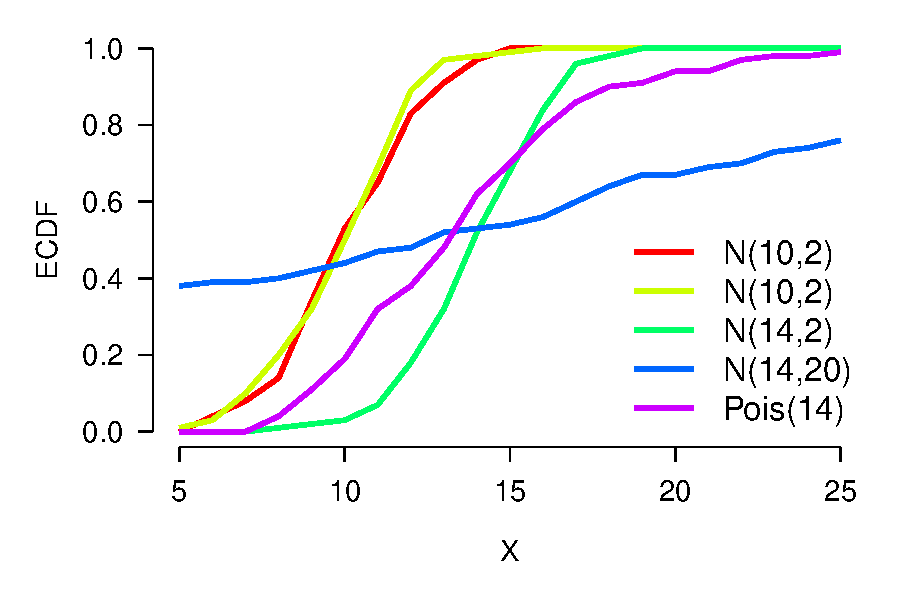
\includegraphics[keepaspectratio]{chapters/ch10_files/figure-pdf/unnamed-chunk-19-1.pdf}}

The KS test results show that distributions \texttt{x1} and \texttt{x2}
are not different (\(p>0.05\)). This makes sense because they are both
normal distributions with the same mean and SD. Distributions
\texttt{x1} and \texttt{x3} are different because they have different
means (10 vs.~14). Distributions \texttt{x3} and \texttt{x4} were
different because they had different SD (2 vs.~20). Finally,
distributions \texttt{x3} and \texttt{x5} were different because they
were different distributions with different shapes (normal vs.~Poisson).

The KS test can be useful when you want to see how well your data
matches up with their theoretical distribution. Consider the example of
a lognormally distributed response below. If we suspect that the data
come from a lognormal distribution or a gamma distribution, we can use
the function \texttt{fitdistr()} to estimate the parameters of a
lognormal and a gamma distribution that are most likely to produce those
data. Then, we use a KS test to compare the data to the idealized
candidates.

\begin{Shaded}
\begin{Highlighting}[]
\CommentTok{\# random number seed}
\FunctionTok{set.seed}\NormalTok{(}\DecValTok{123}\NormalTok{)}

\CommentTok{\# generate data}
\NormalTok{x1 }\OtherTok{\textless{}{-}} \FunctionTok{rlnorm}\NormalTok{(}\DecValTok{100}\NormalTok{, }\DecValTok{2}\NormalTok{, }\DecValTok{2}\NormalTok{)}

\CommentTok{\# estimate moments}
\NormalTok{fit1 }\OtherTok{\textless{}{-}} \FunctionTok{fitdistr}\NormalTok{(x1, }\StringTok{"lognormal"}\NormalTok{)}
\NormalTok{fit2 }\OtherTok{\textless{}{-}} \FunctionTok{fitdistr}\NormalTok{(x1, }\StringTok{"gamma"}\NormalTok{)}
\end{Highlighting}
\end{Shaded}

Notice that the parameters from \texttt{fitdistr()} are supplied as
arguments to \texttt{ks.test()}, following the name of the distribution
we want to compare to. If parameters are not supplied, then R will
perform the KS test using the default parameter values (e.g.,
\texttt{meanlog=0} and \texttt{sdlog=1} for \texttt{plnorm()}; none for
\texttt{pgamma()}), which is not what we want.

\begin{Shaded}
\begin{Highlighting}[]
\FunctionTok{ks.test}\NormalTok{(x1, }\StringTok{"plnorm"}\NormalTok{, fit1}\SpecialCharTok{$}\NormalTok{estimate[}\DecValTok{1}\NormalTok{], fit1}\SpecialCharTok{$}\NormalTok{estimate[}\DecValTok{2}\NormalTok{])}
\end{Highlighting}
\end{Shaded}

\begin{verbatim}

    Asymptotic one-sample Kolmogorov-Smirnov test

data:  x1
D = 0.058719, p-value = 0.8808
alternative hypothesis: two-sided
\end{verbatim}

The test shows that we cannot conclude that \texttt{x1} is different
from a lognormal distribution.

\begin{Shaded}
\begin{Highlighting}[]
\FunctionTok{ks.test}\NormalTok{(x1, }\StringTok{"pgamma"}\NormalTok{, }\AttributeTok{shape=}\NormalTok{fit2}\SpecialCharTok{$}\NormalTok{estimate[}\DecValTok{1}\NormalTok{],}
        \AttributeTok{rate=}\NormalTok{fit2}\SpecialCharTok{$}\NormalTok{estimate[}\DecValTok{2}\NormalTok{])}
\end{Highlighting}
\end{Shaded}

\begin{verbatim}

    Asymptotic one-sample Kolmogorov-Smirnov test

data:  x1
D = 0.16211, p-value = 0.01043
alternative hypothesis: two-sided
\end{verbatim}

The test shows that \texttt{x1} is likely different from a gamma
distribution.

\begin{Shaded}
\begin{Highlighting}[]
\CommentTok{\# plot x1 and its theoretical distribution}
\NormalTok{xx }\OtherTok{\textless{}{-}} \FunctionTok{seq}\NormalTok{(}\FunctionTok{min}\NormalTok{(x1), }\FunctionTok{max}\NormalTok{(x1), }\AttributeTok{length=}\DecValTok{500}\NormalTok{)}
\NormalTok{y1 }\OtherTok{\textless{}{-}} \FunctionTok{ecdf}\NormalTok{(x1)(xx)}
\NormalTok{y2 }\OtherTok{\textless{}{-}} \FunctionTok{plnorm}\NormalTok{(xx, fit1}\SpecialCharTok{$}\NormalTok{estimate[}\DecValTok{1}\NormalTok{], fit1}\SpecialCharTok{$}\NormalTok{estimate[}\DecValTok{2}\NormalTok{])}
\NormalTok{y3 }\OtherTok{\textless{}{-}} \FunctionTok{pgamma}\NormalTok{(xx, }\AttributeTok{shape=}\NormalTok{fit2}\SpecialCharTok{$}\NormalTok{estimate[}\DecValTok{1}\NormalTok{], }\AttributeTok{rate=}\NormalTok{fit2}\SpecialCharTok{$}\NormalTok{estimate[}\DecValTok{2}\NormalTok{])}

\FunctionTok{par}\NormalTok{(}\AttributeTok{mfrow=}\FunctionTok{c}\NormalTok{(}\DecValTok{1}\NormalTok{,}\DecValTok{1}\NormalTok{), }\AttributeTok{mar=}\FunctionTok{c}\NormalTok{(}\FloatTok{5.1}\NormalTok{, }\FloatTok{5.1}\NormalTok{, }\FloatTok{1.1}\NormalTok{, }\FloatTok{1.1}\NormalTok{), }\AttributeTok{bty=}\StringTok{"n"}\NormalTok{, }
    \AttributeTok{las=}\DecValTok{1}\NormalTok{, }\AttributeTok{lend=}\DecValTok{1}\NormalTok{, }\AttributeTok{cex.axis=}\FloatTok{1.2}\NormalTok{, }\AttributeTok{cex.lab=}\FloatTok{1.2}\NormalTok{)}
\FunctionTok{plot}\NormalTok{(}\FunctionTok{log}\NormalTok{(xx), y1, }\AttributeTok{type=}\StringTok{"l"}\NormalTok{, }\AttributeTok{lwd=}\DecValTok{3}\NormalTok{, }\AttributeTok{xlab=}\StringTok{"log(X)"}\NormalTok{, }\AttributeTok{ylab=}\StringTok{"ECDF"}\NormalTok{)}
\FunctionTok{points}\NormalTok{(}\FunctionTok{log}\NormalTok{(xx), y2, }\AttributeTok{type=}\StringTok{"l"}\NormalTok{, }\AttributeTok{lwd=}\DecValTok{3}\NormalTok{, }\AttributeTok{col=}\StringTok{"red"}\NormalTok{)}
\FunctionTok{points}\NormalTok{(}\FunctionTok{log}\NormalTok{(xx), y3, }\AttributeTok{type=}\StringTok{"l"}\NormalTok{, }\AttributeTok{lwd=}\DecValTok{3}\NormalTok{, }\AttributeTok{col=}\StringTok{"blue"}\NormalTok{)}
\FunctionTok{legend}\NormalTok{(}\StringTok{"topleft"}\NormalTok{,}
       \AttributeTok{legend=}\FunctionTok{c}\NormalTok{(}\StringTok{"Data"}\NormalTok{, }\StringTok{"Lognormal"}\NormalTok{, }\StringTok{"Gamma"}\NormalTok{),}
       \AttributeTok{lwd=}\DecValTok{3}\NormalTok{,}
       \AttributeTok{col=}\FunctionTok{c}\NormalTok{(}\StringTok{"black"}\NormalTok{, }\StringTok{"red"}\NormalTok{, }\StringTok{"blue"}\NormalTok{),}
       \AttributeTok{bty=}\StringTok{"n"}\NormalTok{,}
       \AttributeTok{cex=}\FloatTok{1.3}\NormalTok{)}
\end{Highlighting}
\end{Shaded}

\begin{center}
\pandocbounded{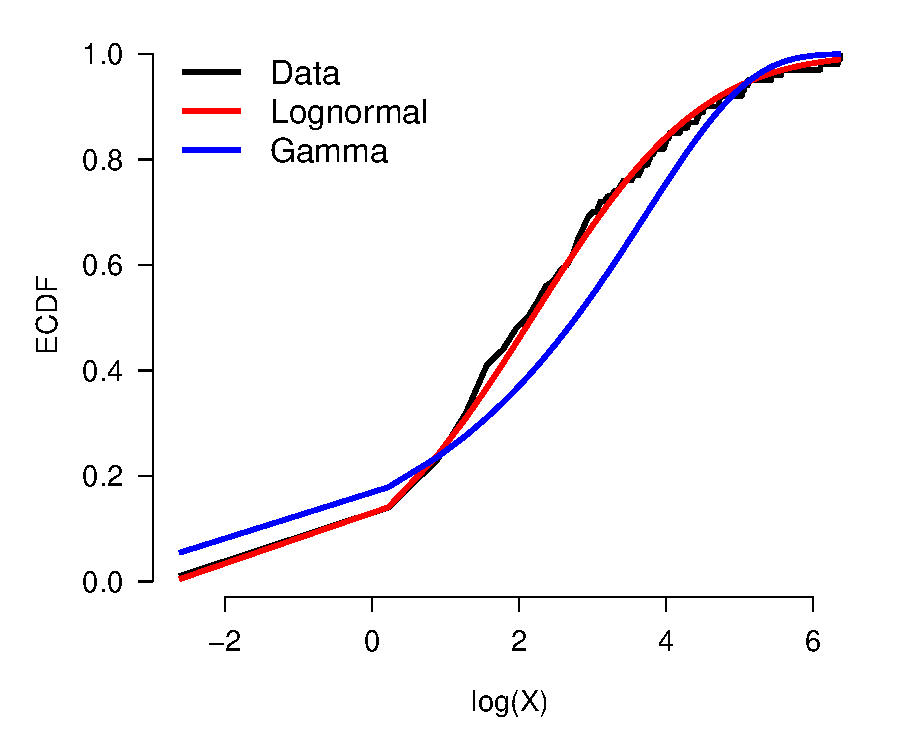
\includegraphics[keepaspectratio]{chapters/ch10_files/figure-pdf/unnamed-chunk-23-1.pdf}}
\end{center}

While neither the lognormal distribution nor the gamma distribution are
awful at representing the data, the KS tests suggest that the simulated
data \texttt{x1} come from a lognormal distribution, not a gamma
distribution. This is because the KS test was non-significant when
comparing the data to the lognormal, and significant when comparing the
data to the gamma distribution. The test comparing the data to the gamma
distribution was, however, close to non-significant (\(p\approx0.01\)).
See what happens if you change the random number seed and re-run the
random generation and the test.

\chapter{Data transformation and rescaling}\label{sec-trans}

\section{Data transformations}\label{sec-trans-trans}

Data transformation is the process of changing the values in your data
according to a function. This is usually done to make the data better
conform to the assumptions of a statistical test, or to make graphs
easier to interpret. Transformation is done to make patterns easier to
detect. In many fields transformations may be standard practice, and
with good reason. Just make sure that you understand what the transform
function is doing, and most importantly, why you are transforming your
data.

\section{Why transform?}\label{sec-trans-why}

\textbf{Data transformation} is the process of applying a function to
your data to change their values. This is usually done so that the data
better conform to the assumptions of a statistical test, or to make
graphs of your data more interpretable. The functions that transform
data are usually called ``transforms''. There are many transforms out
there, but only a few are very common in biology. All convert values on
the \textbf{original scale} to values on the \textbf{transformed scale}.
Variables often have different properties after a transformation, such
as normality, or a different domain, or a different distribution shape.
A function for transforming data must be both \textbf{deterministic} and
\textbf{invertible}:

\begin{itemize}
\tightlist
\item
  \textbf{Deterministic:} the function always returns the same
  transformed value for a given input.
\item
  \textbf{Invertible:} values on the transformed scale can be converted
  unambiguously to values on the original scale.
\end{itemize}

Data transformations are commonly used to make data fit certain
distributions. For example, consider the figure below:

\begin{Shaded}
\begin{Highlighting}[]
\NormalTok{a }\OtherTok{\textless{}{-}} \FunctionTok{rlnorm}\NormalTok{(}\DecValTok{1000}\NormalTok{, }\FloatTok{1.5}\NormalTok{, }\DecValTok{2}\NormalTok{)}
\FunctionTok{par}\NormalTok{(}\AttributeTok{mfrow=}\FunctionTok{c}\NormalTok{(}\DecValTok{1}\NormalTok{,}\DecValTok{2}\NormalTok{))}
\FunctionTok{hist}\NormalTok{(a, }\AttributeTok{main=}\StringTok{"Values on original scale"}\NormalTok{)}
\FunctionTok{hist}\NormalTok{(}\FunctionTok{log}\NormalTok{(a), }\AttributeTok{main=}\StringTok{"Values on transformed scale"}\NormalTok{)}
\end{Highlighting}
\end{Shaded}

\begin{center}
\pandocbounded{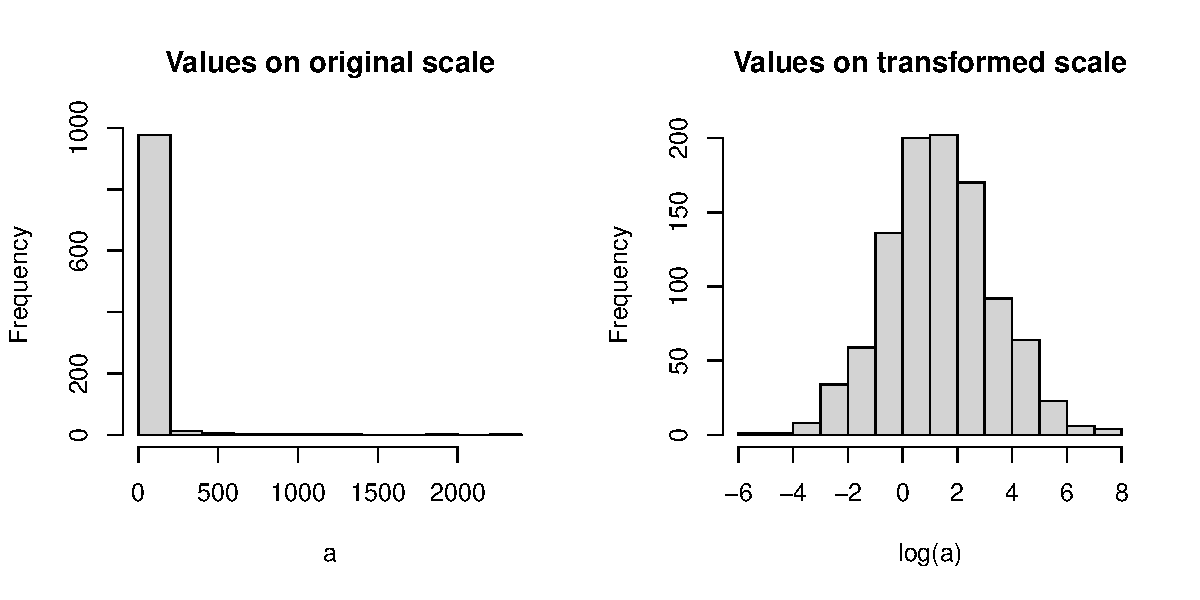
\includegraphics[keepaspectratio]{chapters/ch11_files/figure-pdf/unnamed-chunk-1-1.pdf}}
\end{center}

The left panel shows data with mostly small values and a strong positive
skew. The right panel shows the same data on the log scale. Notice how
the log-transformed values look much more like a normal distribution.
This is very important for many statistical methods, which require
normality in the residuals. The log-transformed plot also lets us see
more details about the distribution that are obscured on the original
scale.

\section{Transforms vs.~link functions}\label{sec-trans-link}

In \href{@sec-glm1}{generalized linear models (GLM)} the response
variable is modeled on a scale defined by a \textbf{link function}. That
link function can look like a transform, and is often confused with a
transform, but there is an important difference.

\begin{itemize}
\tightlist
\item
  A \textbf{transform} changes the observed response variables
  themselves: \(Y\rightarrow g\left(Y\right)\), and the model is fit to
  the transformed observations.
\item
  A \textbf{link function} changes the scale on which the expected value
  of the response is modeled:
  \(g\left(E\left[Y\right]\right)=g\left(\mu\right)\).
\end{itemize}

For example, in a binomial GLM with a logit link,

\[logit\left(p\right)=X\beta\]

you are not literally taking the logit of observed proportions and
fitting a linear regression to those transformed values. The
observations remain binomial, and their variance follows a binomial
distribution.

Thus, fitting \texttt{lm(log(y)\ \textasciitilde{}\ x)} actually
transforms the observed values of \texttt{y}, whereas fitting
\texttt{glm(y\ \textasciitilde{}\ x,\ family=poisson(link="log"))} does
not take the logarithm of the observed values of \texttt{y}.

The figure below shows an example of this: the response variable on its
original scale (left panel), a proportion, is analyzed on the logit
scale (right panel). The deterministic part of the model (the
relationship between the predictors and the response) is linear on the
logit scale, while the stochastic part (the variance) still follows a
binomial distribution on the original scale.

\pandocbounded{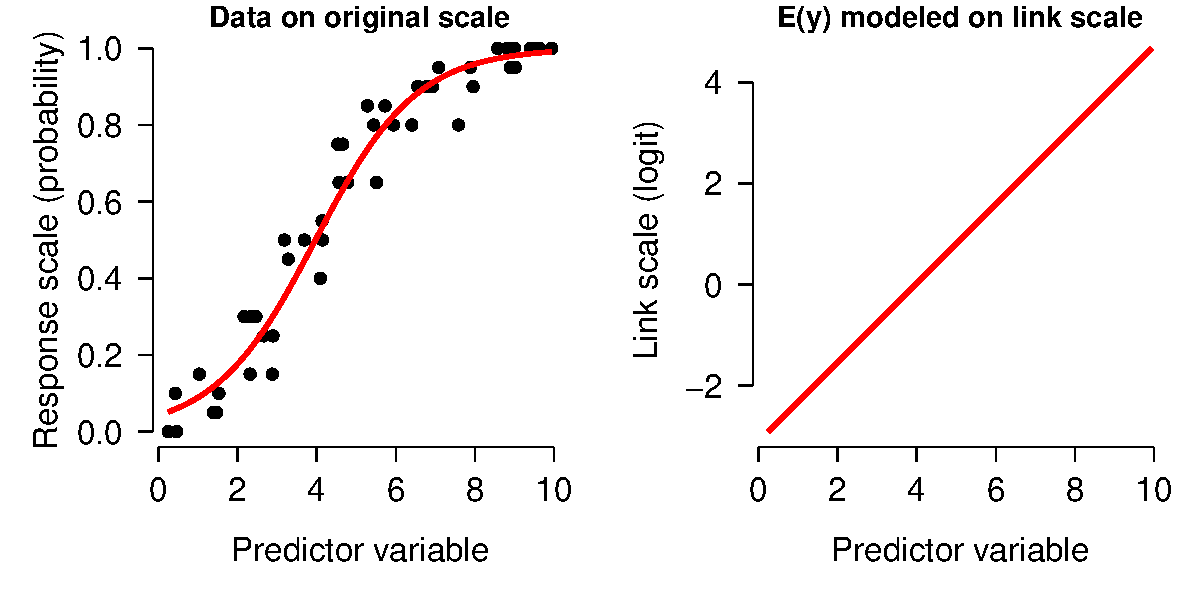
\includegraphics[keepaspectratio]{chapters/ch11_files/figure-pdf/unnamed-chunk-2-1.pdf}}

Let's look at this in another context, because this distinction is
important. \textbf{A GLM link function is not a transformation of the
response variable.} When a response is transformed before fitting a
linear model, the transformed values themselves are modeled, including
their residual variation. In a GLM, the response retains its specified
probability distribution on its original scale; the link function
instead relates the expected value of that distribution to the linear
predictor. The equations below illustrate the difference using two
models that both involve a logarithm.

\textbf{Linear model (LM) with transformation}

In a linear model on transformed data, both the deterministic part of
the model (\(\eta_i = X\beta\)) and the variance
(\(\sigma^2_{residual}\)) are on the transformed scale.

\[y_i = e^{\eta_i}\]

\[\eta_i = X\beta+\varepsilon_i\]

\[\varepsilon_i\sim{Normal}\left(0,\sigma^2_{residual}\right)\]

\textbf{Generalized linear model (GLM) with link function}

In a GLM with a link function, the deterministic part of the model
(\(\eta_i = X\beta\)), while the variance is on the original scale.

\[y_i \sim Normal\left(z_i,\sigma^2_{residual}\right)\]

\[\log{\left(z_i\right)} = \eta_i\]

\[\eta_i = X\beta\]

Notice where the stochasticity appears. In the transformed LM, normally
distributed residual variation is added to \(\log{\left(y_i\right)}\).
In the GLM, observations \(y_i\) are drawn from a normal distribution
with mean \(\mu_i\), variance \(\sigma^2\), and the predictors are
expressed on the log scale. Thus, \texttt{lm(log(y)\textasciitilde{}x)}
and \texttt{glm(y\textasciitilde{}x,\ family=gaussian(link="log"))} are
not equivalent, even though they both involve logarithms.

\section{Common transformations}\label{sec-trans-common}

\subsection{Log transformation}\label{sec-trans-common-log}

The \textbf{log-transform} is one of the most common transforms in
biology. It is simply the \textbf{logarithm of the values}. Recall that
the logarithm is the inverse of exponentiation: if \(a=b^c\), then
\(log_b\left(a \right)=c\). For example, \(\log_2\left(8\right)=3\)
because \(2^3=8\). Most biologists use either the natural logarithm
(\(\log_e\), \(\ln\) or just \(\log\)) or the base-10 logarithm
(\(\log_{10}\)). The choice of base is not that important, because any
log-transform will accomplish the same effect. The default in math and
statistics (and in R) is the natural logarithm. The \textbf{common} or
base-10 logarithm \(\log_{10}\) is also very common in biology and
engineering. Whatever base you use, just be consistent and make it clear
to your audience what you did\footnote{And whatever you do, don't call
  the natural logarithm ``lawn''.}. It is depressingly common to be
unable to use values from old papers because they didn't specify which
base logarithm they used.

There are usually two reasons to use a log-transform:
\textbf{normalization} (i.e., variance stabilization) and
\textbf{positivity}. As \href{@sec-dist-lnorm}{seen in the last module},
many variables that appear non-normal turn out to be normally
distributed on a logarithmic scale. This often occurs when something
about the values is multiplicative in nature. For example, body sizes,
population sizes, and bank account balances are often log-normally
distributed. This is because these quantities tend to grow at a rate
that is proportional to their current size. Transforming to the
logarithmic scale changes multiplicative changes to additive changes.

The figure below shows how values separated by a factor of 2 on the
linear scale map to values separated by 1 (i.e., 20) on the
log\textsubscript{2} scale. Values separated by a common \emph{scaling}
factor on the original scale are mapped to values separated by a common
\emph{additive} constant on the log scale\footnote{\href{https://www.youtube.com/watch?v=VSi0Z04fWj0}{This
  video} illustrates the usefulness of logarithms in statistics
  \textbf{\emph{and}} has a nice theme song.}.

\pandocbounded{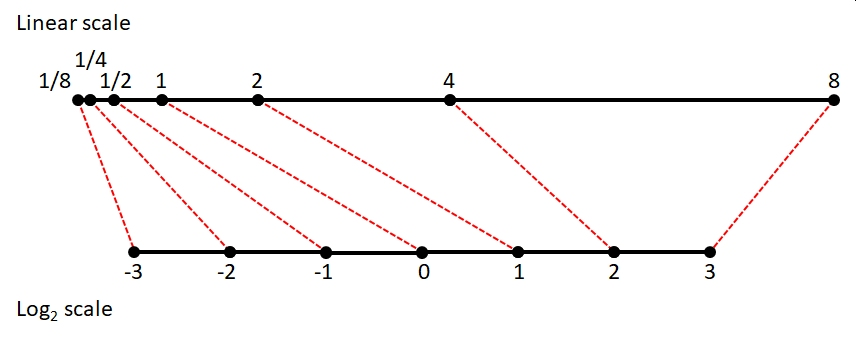
\includegraphics[keepaspectratio,alt={Relationship between a linear scale (top) and logarithmic scale(bottom).}]{chapters/../images/09-01.jpg}}\{alt-text:
``Number line showing how multiplicative changes on a linear scale (top)
become additive changes on a logarithmic scale (bottom). In this
example, one-eigth, one-quarter, one-half, one, two, four, and eight are
mapped to their base 2 logarithms: -3, -2, -1, 0, 1, 2, and 3. Each step
on the linear scale multiplies by 2, but each step on the logarithmic
scale adds 1.''\}

As a side effect of this normalization, log-transformation allows
researchers to work with variables that vary over several orders of
magnitude. This is because scalar multiplication on the untransformed
scale is the same as addition on the log-transformed scale\footnote{Remember
  that exponential functions relate addition and multiplication. This is
  how exponentiation is extended to non-integer powers:
  \(X^aX^b=X^{a+b}\). And, in some sense the \emph{definition} of
  exponentiation.}. The figure below shows how values ranging from 0.001
to 1000 (spanning 6 orders of magnitude) can be managed on the
log-transformed scale.

\pandocbounded{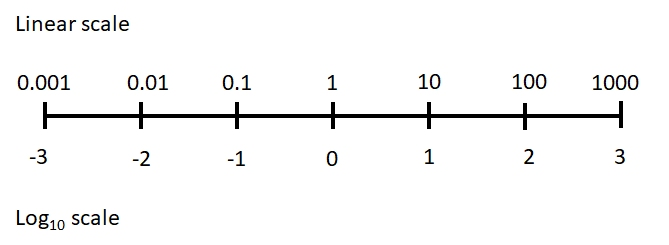
\includegraphics[keepaspectratio,alt={Relationship between a linear scale (top) and logarithmic scale(bottom).}]{chapters/../images/09-02.jpg}}\{alt-text:
``Number line showing how multiplicative changes on a linear scale (top)
become additive changes on a logarithmic scale (bottom). In this
example, 0.001, 0.01, 0.1, 1, 10, 100, and 1000 are mapped to their base
10 logarithms: -3, -2, -1, 0, 1, 2, and 3. Each step on the linear scale
multiplies by 10, but each step on the logarithmic scale adds 1.''\}

The second reason that the log-transform is commonly used is to ensure
that values are always positive. One of the properties of exponents
function is that for any positive base, raising that base to a real
power will always return a positive result. For this reason, it is
common practice to analyze variables with a positive domain either after
a log transform or with a log link function. Such variables include
lengths, masses, and counts, which must be positive or non-negative. Log
transformation can ensure that your analysis does not predict
impossibilities like negative masses.

Values in a data frame can be log-transformed with the \texttt{log()}
(natural log) or \texttt{log10()} (log\textsubscript{10}) function.
Other bases can be used via arguments to the \texttt{log()} function
(e.g., \texttt{log(8,base=2)}). It is usually a good idea to keep the
transformed values in their own variable, rather than overwriting the
original values. This way you can quickly access the original values
without having to back-transform. It is often useful to have the
original values around for making figures. Keeping the original values
also means you don't have to remember whether a variable or object
contains the original or transformed values.

\begin{Shaded}
\begin{Highlighting}[]
\CommentTok{\# spare copy:}
\NormalTok{x }\OtherTok{\textless{}{-}}\NormalTok{ iris}

\CommentTok{\# natural log transform:}
\NormalTok{x}\SpecialCharTok{$}\NormalTok{log.petal.len }\OtherTok{\textless{}{-}} \FunctionTok{log}\NormalTok{(x}\SpecialCharTok{$}\NormalTok{Petal.Length)}

\CommentTok{\# log base 10 transform:}
\NormalTok{x}\SpecialCharTok{$}\NormalTok{log.petal.wid }\OtherTok{\textless{}{-}} \FunctionTok{log10}\NormalTok{(x}\SpecialCharTok{$}\NormalTok{Petal.Width)}
\end{Highlighting}
\end{Shaded}

You can also log-transform many variables at once using the function
\texttt{apply()}. In a data frame this means \texttt{apply}-ing the
\texttt{log()} function to multiple columns (margin 2).

\begin{Shaded}
\begin{Highlighting}[]
\CommentTok{\# load the dataset from package MASS}
\FunctionTok{data}\NormalTok{(crabs, }\AttributeTok{package=}\StringTok{"MASS"}\NormalTok{)}

\CommentTok{\# make a spare copy}
\NormalTok{x }\OtherTok{\textless{}{-}}\NormalTok{ crabs}
\FunctionTok{head}\NormalTok{(x)}
\end{Highlighting}
\end{Shaded}

\begin{verbatim}
  sp sex index   FL  RW   CL   CW  BD
1  B   M     1  8.1 6.7 16.1 19.0 7.0
2  B   M     2  8.8 7.7 18.1 20.8 7.4
3  B   M     3  9.2 7.8 19.0 22.4 7.7
4  B   M     4  9.6 7.9 20.1 23.1 8.2
5  B   M     5  9.8 8.0 20.3 23.0 8.2
6  B   M     6 10.8 9.0 23.0 26.5 9.8
\end{verbatim}

\begin{Shaded}
\begin{Highlighting}[]
\CommentTok{\# overwrite (transform in place)}
\CommentTok{\# (ok but can cause headaches later)}
\NormalTok{x[,}\DecValTok{4}\SpecialCharTok{:}\DecValTok{8}\NormalTok{] }\OtherTok{\textless{}{-}} \FunctionTok{apply}\NormalTok{(x[,}\DecValTok{4}\SpecialCharTok{:}\DecValTok{8}\NormalTok{], }\DecValTok{2}\NormalTok{, log)}
\FunctionTok{head}\NormalTok{(x)}
\end{Highlighting}
\end{Shaded}

\begin{verbatim}
  sp sex index       FL       RW       CL       CW       BD
1  B   M     1 2.091864 1.902108 2.778819 2.944439 1.945910
2  B   M     2 2.174752 2.041220 2.895912 3.034953 2.001480
3  B   M     3 2.219203 2.054124 2.944439 3.109061 2.041220
4  B   M     4 2.261763 2.066863 3.000720 3.139833 2.104134
5  B   M     5 2.282382 2.079442 3.010621 3.135494 2.104134
6  B   M     6 2.379546 2.197225 3.135494 3.277145 2.282382
\end{verbatim}

\begin{Shaded}
\begin{Highlighting}[]
\CommentTok{\# better way:}
\CommentTok{\# make new variables and }
\CommentTok{\# add to original data frame (better)}
\NormalTok{x }\OtherTok{\textless{}{-}}\NormalTok{ crabs}
\NormalTok{z }\OtherTok{\textless{}{-}} \FunctionTok{apply}\NormalTok{(x[,}\DecValTok{4}\SpecialCharTok{:}\DecValTok{8}\NormalTok{], }\DecValTok{2}\NormalTok{, log)}
\NormalTok{z }\OtherTok{\textless{}{-}} \FunctionTok{as.data.frame}\NormalTok{(z)}
\FunctionTok{names}\NormalTok{(z) }\OtherTok{\textless{}{-}} \FunctionTok{paste}\NormalTok{(}\FunctionTok{names}\NormalTok{(z), }\StringTok{"log"}\NormalTok{, }\AttributeTok{sep=}\StringTok{"."}\NormalTok{)}
\NormalTok{x }\OtherTok{\textless{}{-}} \FunctionTok{cbind}\NormalTok{(x,z)}
\FunctionTok{head}\NormalTok{(x)}
\end{Highlighting}
\end{Shaded}

\begin{verbatim}
  sp sex index   FL  RW   CL   CW  BD   FL.log   RW.log   CL.log   CW.log
1  B   M     1  8.1 6.7 16.1 19.0 7.0 2.091864 1.902108 2.778819 2.944439
2  B   M     2  8.8 7.7 18.1 20.8 7.4 2.174752 2.041220 2.895912 3.034953
3  B   M     3  9.2 7.8 19.0 22.4 7.7 2.219203 2.054124 2.944439 3.109061
4  B   M     4  9.6 7.9 20.1 23.1 8.2 2.261763 2.066863 3.000720 3.139833
5  B   M     5  9.8 8.0 20.3 23.0 8.2 2.282382 2.079442 3.010621 3.135494
6  B   M     6 10.8 9.0 23.0 26.5 9.8 2.379546 2.197225 3.135494 3.277145
    BD.log
1 1.945910
2 2.001480
3 2.041220
4 2.104134
5 2.104134
6 2.282382
\end{verbatim}

\subsection{Log transforming with 0 values}\label{sec-trans-common-log0}

One problem that comes up with log-transformation is what to do with
values of 0. The logarithm of 0 is undefined, and returns \(-\infty\) or
\texttt{-Inf} in R. This is usually a problem with counts, rather than
with measurements. The simplest solution is to add a small constant to
the values before transforming. If the smallest nonzero value is 1, then
it is easiest to just add 1 to the values:

\[y_i=\log{\left(x_i+1\right)}\]

This works just fine if the smallest nonzero is approximately 1. Values
between 0 and 1 can cause problems. Adding 1 to these values before
log-transforming will tend to compress the lower end of the distribution
and expand the upper end of the distribution. The R commands below show
this:

\begin{Shaded}
\begin{Highlighting}[]
\NormalTok{x }\OtherTok{\textless{}{-}} \FunctionTok{c}\NormalTok{(}\DecValTok{0}\NormalTok{, }\FloatTok{0.003}\NormalTok{, }\FloatTok{0.03}\NormalTok{, }\FloatTok{0.3}\NormalTok{, }\DecValTok{1}\NormalTok{, }\FloatTok{1.3}\NormalTok{, }\DecValTok{5}\NormalTok{, }\DecValTok{10}\NormalTok{, }\DecValTok{99}\NormalTok{)}
\NormalTok{y }\OtherTok{\textless{}{-}} \FunctionTok{log}\NormalTok{(x}\SpecialCharTok{+}\DecValTok{1}\NormalTok{)}
\FunctionTok{plot}\NormalTok{(x,y, }\AttributeTok{cex=}\FloatTok{1.3}\NormalTok{, }\AttributeTok{pch=}\DecValTok{16}\NormalTok{)}
\end{Highlighting}
\end{Shaded}

\begin{center}
\pandocbounded{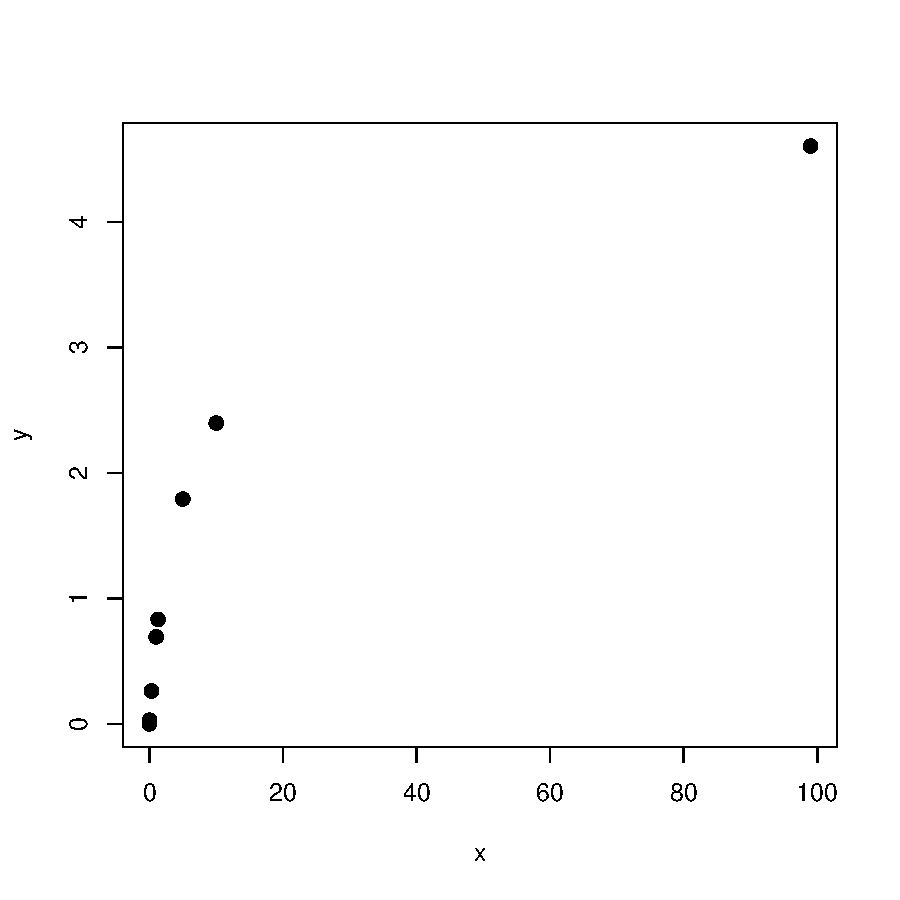
\includegraphics[keepaspectratio]{chapters/ch11_files/figure-pdf/unnamed-chunk-7-1.pdf}}
\end{center}

If the smallest nonzero value differs from 1 by more than an order of
magnitude (i.e., \(\ge10\) or \(\le0.01\)), then a slightly different
procedure is called for. The transformation below generalizes the
\(\log{\left(x+1\right)}\) method so as to result in 0 for 0 values and
somewhat preserve the original orders of magnitude (McCune \emph{et al.}
2002).

\[y_i=\log{\left(x_i+d\right)}-c\]

In this equation:

\[\begin{matrix}c=&Trunc\left(\log{\left(min\left(x\right)\right)}\right)\\d=&e^c\\min\left(x\right)=&smallest\ nonzero\ x\\Trunc\left(x\right)=&function\ that\ truncates\ x\ to\ an\ integer\\\end{matrix}\]

This can be implemented in R using the following custom function:

\begin{Shaded}
\begin{Highlighting}[]
\NormalTok{mgtrans }\OtherTok{\textless{}{-}} \ControlFlowTok{function}\NormalTok{(x)\{}
\NormalTok{    minx }\OtherTok{\textless{}{-}} \FunctionTok{min}\NormalTok{(x[x }\SpecialCharTok{\textgreater{}} \DecValTok{0}\NormalTok{])}
\NormalTok{    cons }\OtherTok{\textless{}{-}} \FunctionTok{trunc}\NormalTok{(}\FunctionTok{log}\NormalTok{(minx))}
\NormalTok{    y }\OtherTok{\textless{}{-}} \FunctionTok{log}\NormalTok{(x }\SpecialCharTok{+} \FunctionTok{exp}\NormalTok{(cons)) }\SpecialCharTok{{-}}\NormalTok{ cons}
    \FunctionTok{return}\NormalTok{(y)}
\NormalTok{\}}

\CommentTok{\# example usage:}
\NormalTok{a }\OtherTok{\textless{}{-}} \FunctionTok{c}\NormalTok{(}\DecValTok{0}\NormalTok{, }\FunctionTok{rlnorm}\NormalTok{(}\DecValTok{9}\NormalTok{))}
\FunctionTok{log}\NormalTok{(a)}
\end{Highlighting}
\end{Shaded}

\begin{verbatim}
 [1]        -Inf  0.25331851 -0.02854676 -0.04287046  1.36860228 -0.22577099
 [7]  1.51647060 -1.54875280  0.58461375  0.12385424
\end{verbatim}

\begin{Shaded}
\begin{Highlighting}[]
\FunctionTok{mgtrans}\NormalTok{(a)}
\end{Highlighting}
\end{Shaded}

\begin{verbatim}
 [1] 0.000000 1.504510 1.292473 1.282103 2.458088 1.153391 2.594120 0.455949
 [9] 1.771116 1.405285
\end{verbatim}

\begin{Shaded}
\begin{Highlighting}[]
\CommentTok{\# count the points:}
\FunctionTok{par}\NormalTok{(}\AttributeTok{mfrow=}\FunctionTok{c}\NormalTok{(}\DecValTok{1}\NormalTok{,}\DecValTok{2}\NormalTok{))}
\FunctionTok{plot}\NormalTok{(a, }\FunctionTok{log}\NormalTok{(a))     }\CommentTok{\# missing one!}
\FunctionTok{plot}\NormalTok{(a, }\FunctionTok{mgtrans}\NormalTok{(a))}
\end{Highlighting}
\end{Shaded}

\pandocbounded{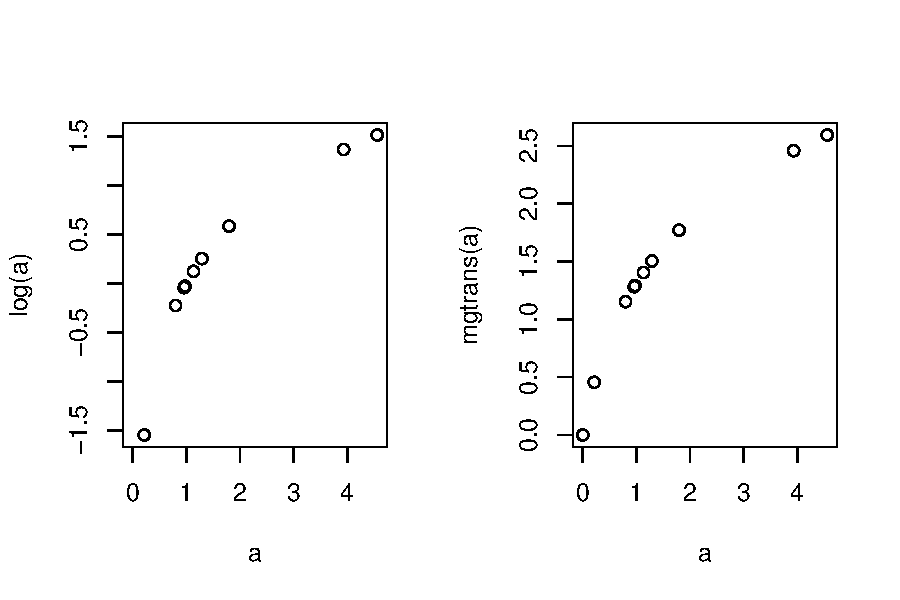
\includegraphics[keepaspectratio]{chapters/ch11_files/figure-pdf/unnamed-chunk-10-1.pdf}}

Note that if you use the McCune and Grace transform, you should keep the
original values around for plotting because back-transforming can be
tricky (if not impossible, if you don't know \emph{d} and \emph{c}). If
you are going to back-transform other values, such as model predictions,
you will need to know \emph{d} and \emph{c}.

The example below shows how the McCune and Grace transform can be
advantageous. First, we create 1000 random values from a lognormal
distribution. Then, randomly set 100 of the values to 0.
Log-transforming the data to achieve normality comes at the cost of
losing 10\% of the values because \texttt{log(0)} is undefined (left
panel). The \(\log\left(x+1\right)\) transform retains all of the
values, but distorts the shape of the distribution (middle panel)
because many values are between 0 and 1. The McCune and Grace method
(right panel) achieves normality (mostly) \emph{and} retains all values.

\begin{Shaded}
\begin{Highlighting}[]
\FunctionTok{set.seed}\NormalTok{(}\DecValTok{123}\NormalTok{)}
\NormalTok{n }\OtherTok{\textless{}{-}} \FloatTok{1e3}
\NormalTok{x }\OtherTok{\textless{}{-}} \FunctionTok{rlnorm}\NormalTok{(n, }\FloatTok{0.5}\NormalTok{, }\DecValTok{1}\NormalTok{)}
\NormalTok{x[}\FunctionTok{sample}\NormalTok{(}\DecValTok{1}\SpecialCharTok{:}\NormalTok{n, }\DecValTok{100}\NormalTok{, }\AttributeTok{replace=}\ConstantTok{FALSE}\NormalTok{)] }\OtherTok{\textless{}{-}} \DecValTok{0}


\NormalTok{t1 }\OtherTok{\textless{}{-}} \FunctionTok{log}\NormalTok{(x)}
\NormalTok{t2 }\OtherTok{\textless{}{-}} \FunctionTok{log}\NormalTok{(x}\SpecialCharTok{+}\DecValTok{1}\NormalTok{)}
\NormalTok{t3 }\OtherTok{\textless{}{-}} \FunctionTok{mgtrans}\NormalTok{(x)}

\FunctionTok{length}\NormalTok{(}\FunctionTok{which}\NormalTok{(}\FunctionTok{is.finite}\NormalTok{(t1)))}
\end{Highlighting}
\end{Shaded}

\begin{verbatim}
[1] 900
\end{verbatim}

\begin{Shaded}
\begin{Highlighting}[]
\FunctionTok{par}\NormalTok{(}\AttributeTok{mfrow=}\FunctionTok{c}\NormalTok{(}\DecValTok{1}\NormalTok{,}\DecValTok{3}\NormalTok{), }\AttributeTok{cex.main=}\FloatTok{1.2}\NormalTok{)}
\FunctionTok{hist}\NormalTok{(t1, }\AttributeTok{main=}\FunctionTok{expression}\NormalTok{(Log}\SpecialCharTok{\textasciitilde{}}\NormalTok{transform}\SpecialCharTok{\textasciitilde{}}\NormalTok{(}\FunctionTok{italic}\NormalTok{(n)}\SpecialCharTok{==}\DecValTok{900}\NormalTok{)))}
\FunctionTok{hist}\NormalTok{(t2, }\AttributeTok{main=}\FunctionTok{expression}\NormalTok{(Log}\SpecialCharTok{\textasciitilde{}}\NormalTok{(}\FunctionTok{italic}\NormalTok{(x)}\SpecialCharTok{+}\DecValTok{1}\NormalTok{)}\SpecialCharTok{\textasciitilde{}}\NormalTok{transform}\SpecialCharTok{\textasciitilde{}}\NormalTok{(}\FunctionTok{italic}\NormalTok{(n)}\SpecialCharTok{==}\DecValTok{1000}\NormalTok{)))}
\FunctionTok{hist}\NormalTok{(t3, }\AttributeTok{main=}\FunctionTok{expression}\NormalTok{(McCune}\SpecialCharTok{{-}}\NormalTok{Grace}\SpecialCharTok{\textasciitilde{}}\NormalTok{transform}\SpecialCharTok{\textasciitilde{}}\NormalTok{(}\FunctionTok{italic}\NormalTok{(n)}\SpecialCharTok{==}\DecValTok{1000}\NormalTok{)))}
\end{Highlighting}
\end{Shaded}

\pandocbounded{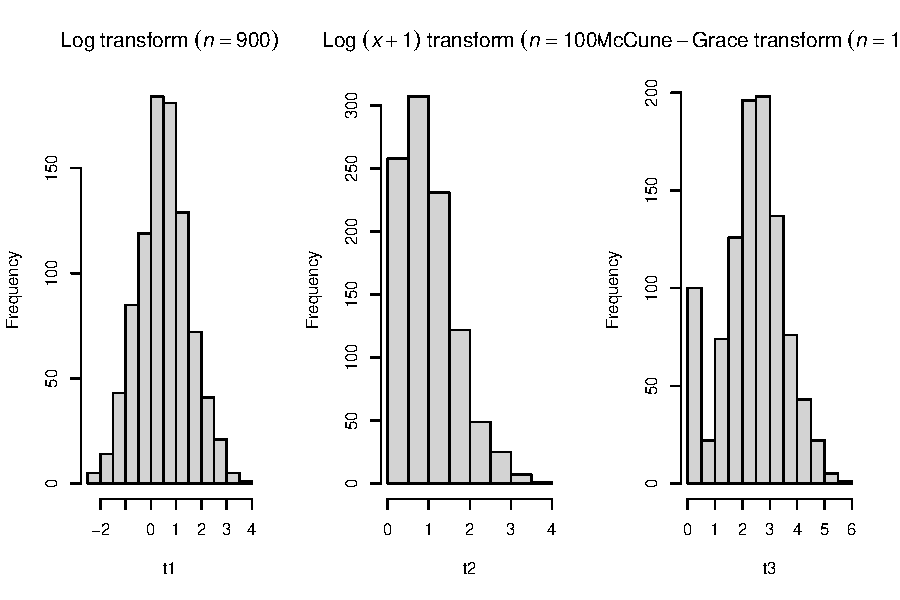
\includegraphics[keepaspectratio]{chapters/ch11_files/figure-pdf/unnamed-chunk-12-1.pdf}}

The spike in the right histogram comes from the fact that the McCune and
Grace method maps values of 0 to 0.

\subsection{Rank transformation}\label{sec-trans-common-rank}

The \textbf{rank transform} replaces values with their ranks. The R
function for this is \texttt{rank()}. Smaller values having smaller
ranks and greater values having greater ranks. The smallest value has
rank = 1, and the largest value has a rank equal to the number of
values. That is, for any vector x \texttt{rank(x){[}x==min(x){]}} = 1
and \texttt{rank(x){[}x==max(x){]}} = \texttt{length(x)}.

\begin{Shaded}
\begin{Highlighting}[]
\NormalTok{x }\OtherTok{\textless{}{-}} \FunctionTok{rnorm}\NormalTok{(}\DecValTok{20}\NormalTok{, }\DecValTok{5}\NormalTok{, }\DecValTok{1}\NormalTok{)}
\NormalTok{y }\OtherTok{\textless{}{-}} \FunctionTok{rank}\NormalTok{(x)}

\FunctionTok{par}\NormalTok{(}\AttributeTok{mfrow=}\FunctionTok{c}\NormalTok{(}\DecValTok{1}\NormalTok{,}\DecValTok{1}\NormalTok{))}
\FunctionTok{plot}\NormalTok{(x,y, }\AttributeTok{xlab=}\StringTok{"Values"}\NormalTok{, }\AttributeTok{ylab=}\StringTok{"Rank(Values)"}\NormalTok{)}
\end{Highlighting}
\end{Shaded}

\begin{center}
\pandocbounded{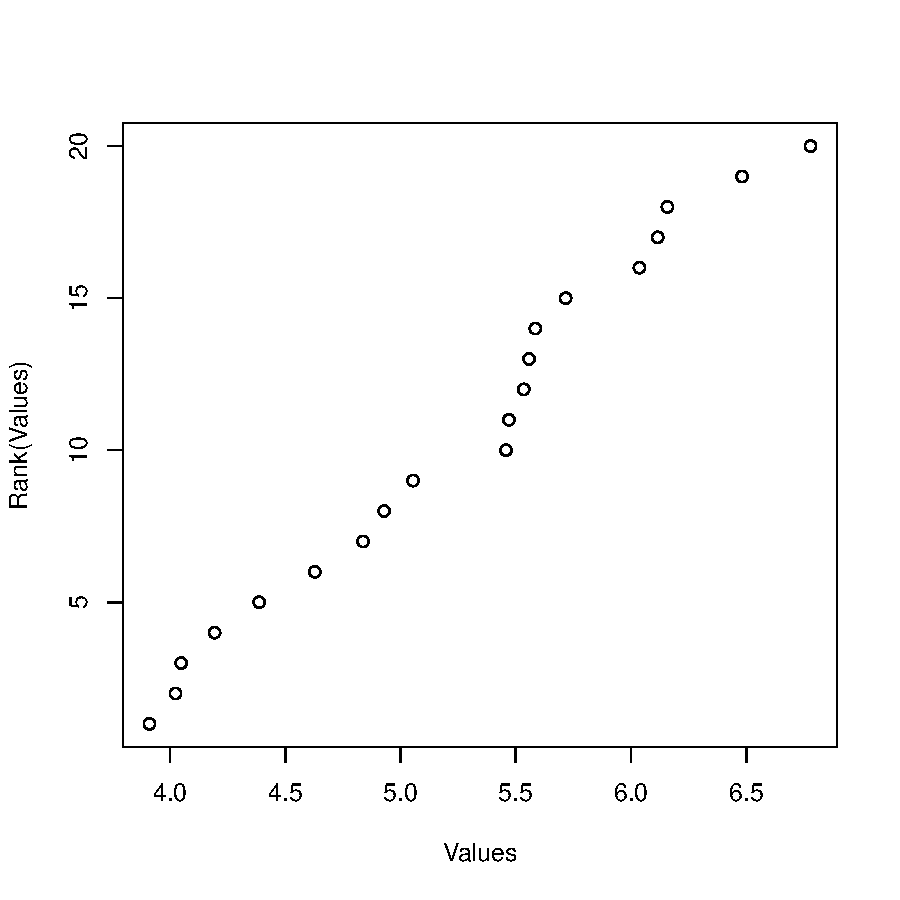
\includegraphics[keepaspectratio]{chapters/ch11_files/figure-pdf/unnamed-chunk-13-1.pdf}}
\end{center}

Notice how the transformed variables \texttt{y} are evenly spaced while
the original values are not. This can be useful if values are very
``clumped'' or ``spread out''. Rank transforms are commonly used in
nonparametric procedures. Note that the \texttt{rank()} function may
return fractional or repeated ranks if there are ties:

\begin{Shaded}
\begin{Highlighting}[]
\CommentTok{\# make some random values}
\NormalTok{x }\OtherTok{\textless{}{-}} \FunctionTok{runif}\NormalTok{(}\DecValTok{10}\NormalTok{)}

\CommentTok{\# force a tie}
\NormalTok{x[}\DecValTok{1}\NormalTok{] }\OtherTok{\textless{}{-}}\NormalTok{ x[}\DecValTok{2}\NormalTok{]}

\CommentTok{\# fractional ranks for ties:}
\FunctionTok{rank}\NormalTok{(x)}
\end{Highlighting}
\end{Shaded}

\begin{verbatim}
 [1]  1.5  1.5  4.0  6.0  7.0  9.0  5.0 10.0  8.0  3.0
\end{verbatim}

\begin{Shaded}
\begin{Highlighting}[]
\CommentTok{\# force a three{-}way tie:}
\NormalTok{x[}\DecValTok{3}\NormalTok{] }\OtherTok{\textless{}{-}}\NormalTok{ x[}\DecValTok{2}\NormalTok{]}

\CommentTok{\# repeated ranks:}
\FunctionTok{rank}\NormalTok{(x)}
\end{Highlighting}
\end{Shaded}

\begin{verbatim}
 [1]  2  2  2  6  7  9  5 10  8  4
\end{verbatim}

\subsection{Logit and probit transformations}\label{sec-trans-common-lp}

\subsubsection{Logit transformation}\label{sec-trans-common-lp-logit}

The \textbf{logit transformation} and \textbf{probit transformation} are
used to map \textbf{proportions} to the \textbf{real number line}. Often
this changes proportions into something resembling a normal
distribution. The \textbf{logit} is defined as the \emph{logarithm of
the odds ratio}. For any value \emph{x} in the open interval\footnote{An
  \textbf{open interval} is an interval \(\left(a,b\right)\) that
  contains values \(>a\) and \(<b\), but never \(a\) or \(b\). Open
  intervals are denoted by parentheses (). Intervals that contain their
  limits are called \textbf{closed intervals}, denoted with brackets
  {[}{]}: \(\left[a,b\right]\).} (0, 1), the logit is calculated as:

\[logit\left(x\right)=\log{\left(\frac{x}{1-x}\right)}\]

The inverse of the logit function is the \textbf{logistic function}.

\[logistic\left(x\right)=\frac{e^x}{e^x+1}=\frac{1}{1+e^{-x}}\]

If \emph{x} is a probability or proportion, then logit(\emph{x}) is the
logarithm of the odds ratio. For this reason, the logit is also called
the ``log-odds''. The logit function is also the inverse of the logistic
function.

The figure below shows the relationship between the logit and logistic
functions:

\pandocbounded{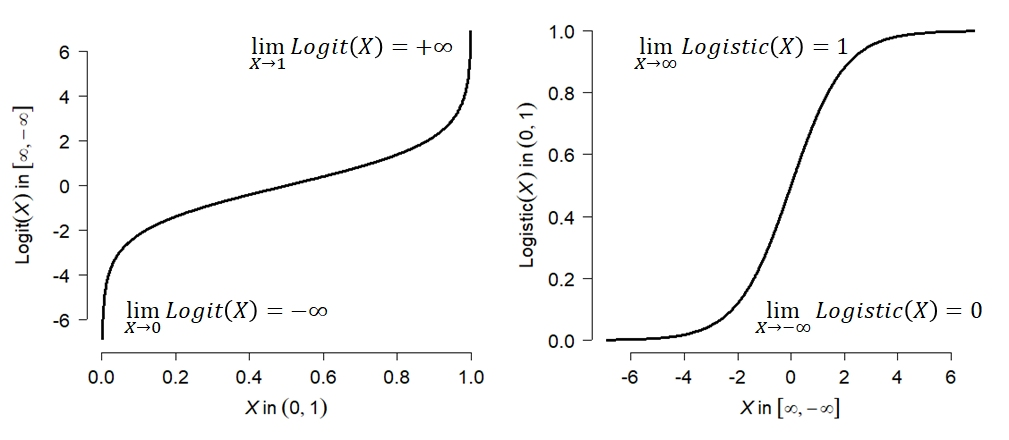
\includegraphics[keepaspectratio,alt={The logit and logistic functions. The logit function (left) maps probabilities in the interval \textbackslash left(0,1\textbackslash right) onto the unbounded interval \textbackslash left(−\textbackslash infty,+\textbackslash infty). The logistic function (right) is its inverse, mapping values from \textbackslash left(−\textbackslash infty,+\textbackslash infty) back onto \textbackslash left(0,1\textbackslash right).}]{chapters/../images/09-03.jpg}}\{fig-alt:
``Two plots illustrating inverse functions. The logit function increases
from negative infinity as X approaches 0 to positive infinity as X
approaches 1, crossing zero at X=0.5. The logistic function is an
S-shaped curve increasing from 0 to 1 as X ranges from negative to
positive infinity, crossing 0.5 at X=0.''\}

The logit transformation has the effect of stretching out the ends of a
distribution, while keeping the relationship between the original and
transformed values roughly linear near the middle of the distribution.
The logit transformation can be accomplished in R using the function
\texttt{qlogis()}; its inverse, the logistic function, is
\texttt{plogis()}.

\begin{Shaded}
\begin{Highlighting}[]
\NormalTok{x }\OtherTok{\textless{}{-}} \DecValTok{1}\SpecialCharTok{:}\DecValTok{999}\SpecialCharTok{/}\DecValTok{1000}
\NormalTok{y }\OtherTok{\textless{}{-}} \FunctionTok{qlogis}\NormalTok{(x)}

\CommentTok{\# compare:}
\FunctionTok{par}\NormalTok{(}\AttributeTok{mfrow=}\FunctionTok{c}\NormalTok{(}\DecValTok{1}\NormalTok{,}\DecValTok{2}\NormalTok{))}
\FunctionTok{hist}\NormalTok{(x)}
\FunctionTok{hist}\NormalTok{(y)}
\end{Highlighting}
\end{Shaded}

\begin{center}
\pandocbounded{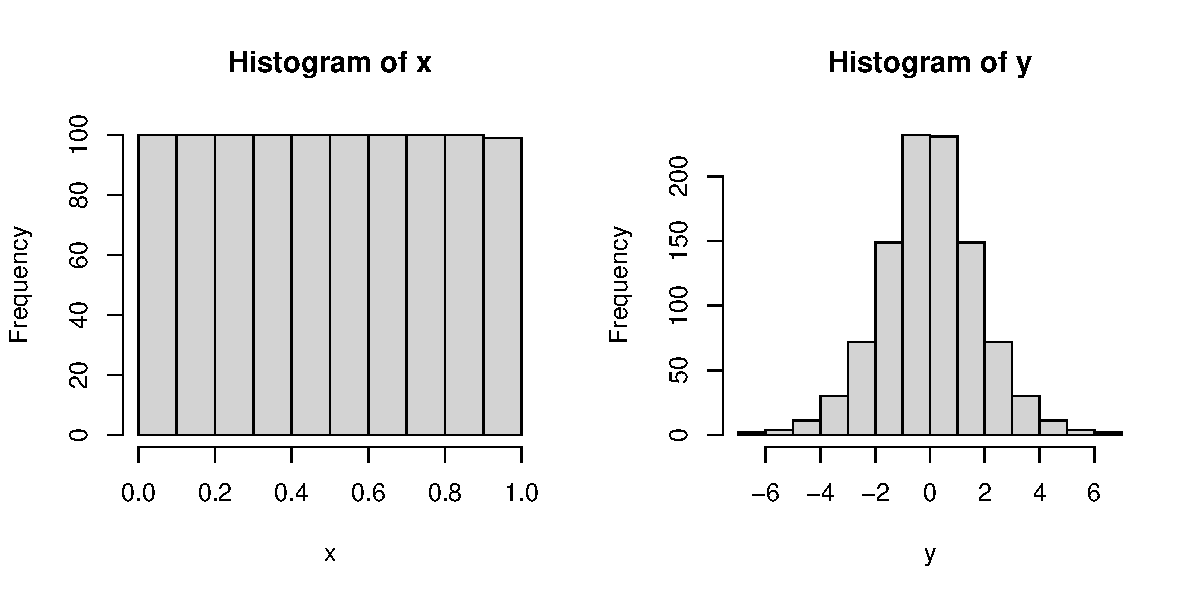
\includegraphics[keepaspectratio]{chapters/ch11_files/figure-pdf/unnamed-chunk-16-1.pdf}}
\end{center}

Why is this useful? The logistic function takes any real input and
outputs a value between 0 and 1. This means that the logit function
takes values between 0 and 1 and outputs a real number. The example
below shows how this can be applied to analyze proportions:

The first figure below shows how analyzing proportions with linear
models leads to clearly inappropriate results. The predicted values of
the model extend well outside the possible range of a probability.

\begin{Shaded}
\begin{Highlighting}[]
\FunctionTok{set.seed}\NormalTok{(}\DecValTok{123}\NormalTok{)}
\NormalTok{n }\OtherTok{\textless{}{-}} \DecValTok{50}
\NormalTok{x }\OtherTok{\textless{}{-}} \FunctionTok{runif}\NormalTok{(n, }\DecValTok{0}\NormalTok{, }\DecValTok{10}\NormalTok{)}
\NormalTok{z }\OtherTok{\textless{}{-}} \SpecialCharTok{{-}}\DecValTok{3} \SpecialCharTok{+} \FloatTok{0.75}\SpecialCharTok{*}\NormalTok{x }\SpecialCharTok{+} \FunctionTok{rnorm}\NormalTok{(n, }\DecValTok{0}\NormalTok{, }\DecValTok{1}\NormalTok{)}
\NormalTok{y }\OtherTok{\textless{}{-}} \FunctionTok{plogis}\NormalTok{(z)}

\NormalTok{mod1 }\OtherTok{\textless{}{-}} \FunctionTok{lm}\NormalTok{(y}\SpecialCharTok{\textasciitilde{}}\NormalTok{x)}
\NormalTok{px }\OtherTok{\textless{}{-}} \FunctionTok{seq}\NormalTok{(}\FunctionTok{min}\NormalTok{(x), }\FunctionTok{max}\NormalTok{(x), }\AttributeTok{length=}\DecValTok{100}\NormalTok{)}
\NormalTok{pred }\OtherTok{\textless{}{-}} \FunctionTok{predict}\NormalTok{(mod1, }\AttributeTok{newdata=}\FunctionTok{data.frame}\NormalTok{(}\AttributeTok{x=}\NormalTok{px), }\AttributeTok{se.fit=}\ConstantTok{TRUE}\NormalTok{)}
\NormalTok{mn }\OtherTok{\textless{}{-}}\NormalTok{ pred}\SpecialCharTok{$}\NormalTok{fit}
\NormalTok{lo }\OtherTok{\textless{}{-}} \FunctionTok{qnorm}\NormalTok{(}\FloatTok{0.025}\NormalTok{, mn, pred}\SpecialCharTok{$}\NormalTok{se.fit) }
\NormalTok{up }\OtherTok{\textless{}{-}} \FunctionTok{qnorm}\NormalTok{(}\FloatTok{0.975}\NormalTok{, mn, pred}\SpecialCharTok{$}\NormalTok{se.fit)}

\FunctionTok{par}\NormalTok{(}\AttributeTok{mfrow=}\FunctionTok{c}\NormalTok{(}\DecValTok{1}\NormalTok{,}\DecValTok{1}\NormalTok{))}
\FunctionTok{plot}\NormalTok{(x, y, }\AttributeTok{ylim=}\FunctionTok{c}\NormalTok{(}\DecValTok{0}\NormalTok{, }\FloatTok{1.3}\NormalTok{))}
\FunctionTok{segments}\NormalTok{(}\DecValTok{0}\NormalTok{, }\DecValTok{1}\NormalTok{, }\DecValTok{10}\NormalTok{, }\DecValTok{1}\NormalTok{, }\AttributeTok{lty=}\DecValTok{2}\NormalTok{)}
\FunctionTok{segments}\NormalTok{(}\DecValTok{0}\NormalTok{, }\DecValTok{0}\NormalTok{, }\DecValTok{10}\NormalTok{, }\DecValTok{0}\NormalTok{, }\AttributeTok{lty=}\DecValTok{2}\NormalTok{)}
\FunctionTok{points}\NormalTok{(px, mn, }\AttributeTok{type=}\StringTok{"l"}\NormalTok{, }\AttributeTok{lwd=}\DecValTok{2}\NormalTok{, }\AttributeTok{col=}\StringTok{"red"}\NormalTok{)}
\FunctionTok{points}\NormalTok{(px, lo, }\AttributeTok{type=}\StringTok{"l"}\NormalTok{, }\AttributeTok{lwd=}\DecValTok{2}\NormalTok{, }\AttributeTok{lty=}\DecValTok{2}\NormalTok{, }\AttributeTok{col=}\StringTok{"red"}\NormalTok{)}
\FunctionTok{points}\NormalTok{(px, up, }\AttributeTok{type=}\StringTok{"l"}\NormalTok{, }\AttributeTok{lwd=}\DecValTok{2}\NormalTok{, }\AttributeTok{lty=}\DecValTok{2}\NormalTok{, }\AttributeTok{col=}\StringTok{"red"}\NormalTok{)}
\end{Highlighting}
\end{Shaded}

\begin{center}
\pandocbounded{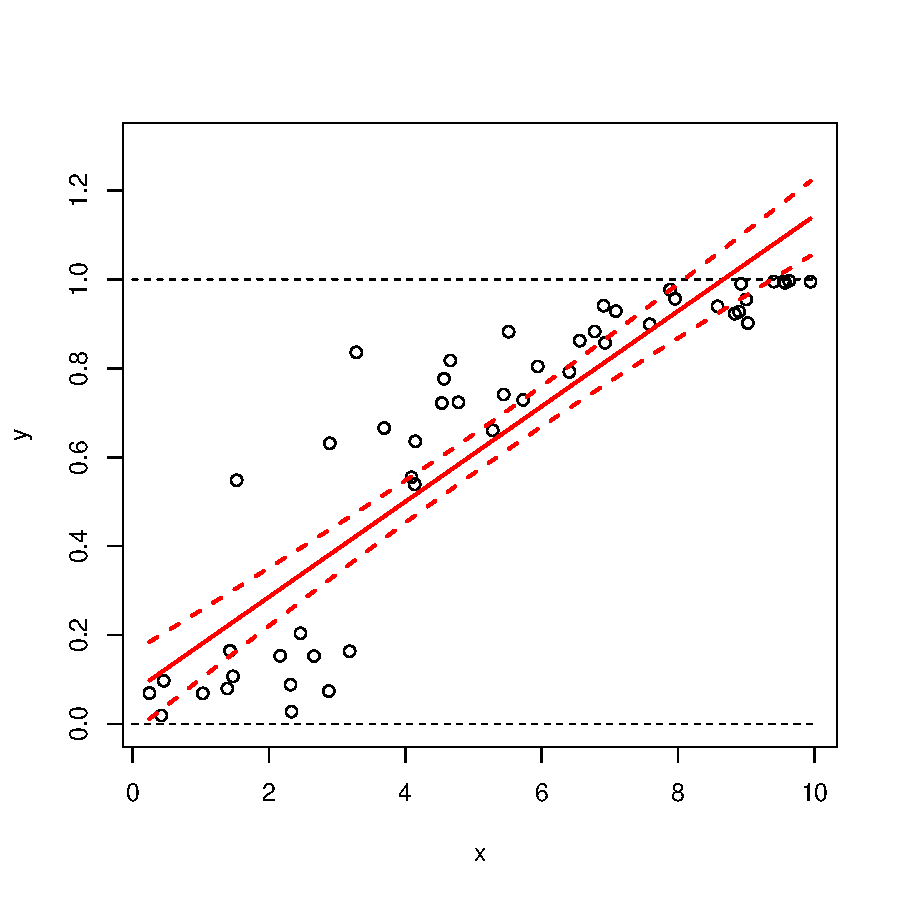
\includegraphics[keepaspectratio]{chapters/ch11_files/figure-pdf/unnamed-chunk-17-1.pdf}}
\end{center}

The linear model predicts probabilities (\texttt{y}) less than 0 and
greater than 1, so clearly it is inappropriate for analyzing
probabilities. However, applying a logit transform to the data for
analysis (and later back-transforming using the logistic function) can
allow you to analyze proportions. Another (and sometimes better way) to
accomplish this is to use a \href{@sec-glm4-binom}{GLM with binomial
family and logit link}.

\begin{Shaded}
\begin{Highlighting}[]
\NormalTok{y2 }\OtherTok{\textless{}{-}} \FunctionTok{qlogis}\NormalTok{(y)}
\NormalTok{mod2 }\OtherTok{\textless{}{-}} \FunctionTok{lm}\NormalTok{(y2}\SpecialCharTok{\textasciitilde{}}\NormalTok{x)}
\NormalTok{pred2 }\OtherTok{\textless{}{-}} \FunctionTok{predict}\NormalTok{(mod2, }\AttributeTok{newdata=}\FunctionTok{data.frame}\NormalTok{(}\AttributeTok{x=}\NormalTok{px), }\AttributeTok{se.fit=}\ConstantTok{TRUE}\NormalTok{)}
\NormalTok{mn2 }\OtherTok{\textless{}{-}}\NormalTok{ pred2}\SpecialCharTok{$}\NormalTok{fit}
\NormalTok{lo2 }\OtherTok{\textless{}{-}} \FunctionTok{qnorm}\NormalTok{(}\FloatTok{0.025}\NormalTok{, mn2, pred2}\SpecialCharTok{$}\NormalTok{se.fit) }
\NormalTok{up2 }\OtherTok{\textless{}{-}} \FunctionTok{qnorm}\NormalTok{(}\FloatTok{0.975}\NormalTok{, mn2, pred2}\SpecialCharTok{$}\NormalTok{se.fit)}
\CommentTok{\# backtransform}
\NormalTok{mn2 }\OtherTok{\textless{}{-}} \FunctionTok{plogis}\NormalTok{(mn2)}
\NormalTok{lo2 }\OtherTok{\textless{}{-}} \FunctionTok{plogis}\NormalTok{(lo2)}
\NormalTok{up2 }\OtherTok{\textless{}{-}} \FunctionTok{plogis}\NormalTok{(up2)}

\FunctionTok{par}\NormalTok{(}\AttributeTok{mfrow=}\FunctionTok{c}\NormalTok{(}\DecValTok{1}\NormalTok{,}\DecValTok{1}\NormalTok{))}
\FunctionTok{plot}\NormalTok{(x, y, }\AttributeTok{ylim=}\FunctionTok{c}\NormalTok{(}\DecValTok{0}\NormalTok{, }\FloatTok{1.3}\NormalTok{))}
\FunctionTok{segments}\NormalTok{(}\DecValTok{0}\NormalTok{, }\DecValTok{1}\NormalTok{, }\DecValTok{10}\NormalTok{, }\DecValTok{1}\NormalTok{, }\AttributeTok{lty=}\DecValTok{2}\NormalTok{)}
\FunctionTok{segments}\NormalTok{(}\DecValTok{0}\NormalTok{, }\DecValTok{0}\NormalTok{, }\DecValTok{10}\NormalTok{, }\DecValTok{0}\NormalTok{, }\AttributeTok{lty=}\DecValTok{2}\NormalTok{)}
\FunctionTok{points}\NormalTok{(px, mn, }\AttributeTok{type=}\StringTok{"l"}\NormalTok{, }\AttributeTok{lwd=}\DecValTok{2}\NormalTok{, }\AttributeTok{col=}\StringTok{"red"}\NormalTok{)}
\FunctionTok{points}\NormalTok{(px, lo, }\AttributeTok{type=}\StringTok{"l"}\NormalTok{, }\AttributeTok{lwd=}\DecValTok{2}\NormalTok{, }\AttributeTok{lty=}\DecValTok{2}\NormalTok{, }\AttributeTok{col=}\StringTok{"red"}\NormalTok{)}
\FunctionTok{points}\NormalTok{(px, up, }\AttributeTok{type=}\StringTok{"l"}\NormalTok{, }\AttributeTok{lwd=}\DecValTok{2}\NormalTok{, }\AttributeTok{lty=}\DecValTok{2}\NormalTok{, }\AttributeTok{col=}\StringTok{"red"}\NormalTok{)}
\FunctionTok{points}\NormalTok{(px, mn2, }\AttributeTok{type=}\StringTok{"l"}\NormalTok{, }\AttributeTok{lwd=}\DecValTok{2}\NormalTok{, }\AttributeTok{col=}\StringTok{"blue"}\NormalTok{)}
\FunctionTok{points}\NormalTok{(px, lo2, }\AttributeTok{type=}\StringTok{"l"}\NormalTok{, }\AttributeTok{lwd=}\DecValTok{2}\NormalTok{, }\AttributeTok{lty=}\DecValTok{2}\NormalTok{, }\AttributeTok{col=}\StringTok{"blue"}\NormalTok{)}
\FunctionTok{points}\NormalTok{(px, up2, }\AttributeTok{type=}\StringTok{"l"}\NormalTok{, }\AttributeTok{lwd=}\DecValTok{2}\NormalTok{, }\AttributeTok{lty=}\DecValTok{2}\NormalTok{, }\AttributeTok{col=}\StringTok{"blue"}\NormalTok{)}
\FunctionTok{legend}\NormalTok{(}\StringTok{"bottomright"}\NormalTok{, }
       \AttributeTok{legend=}\FunctionTok{c}\NormalTok{(}\StringTok{"Linear"}\NormalTok{, }\StringTok{"Logit{-}transformed"}\NormalTok{),}
       \AttributeTok{lwd=}\DecValTok{2}\NormalTok{, }\AttributeTok{col=}\FunctionTok{c}\NormalTok{(}\StringTok{"red"}\NormalTok{, }\StringTok{"blue"}\NormalTok{), }\AttributeTok{bg=}\StringTok{"white"}\NormalTok{)}
\end{Highlighting}
\end{Shaded}

\begin{center}
\pandocbounded{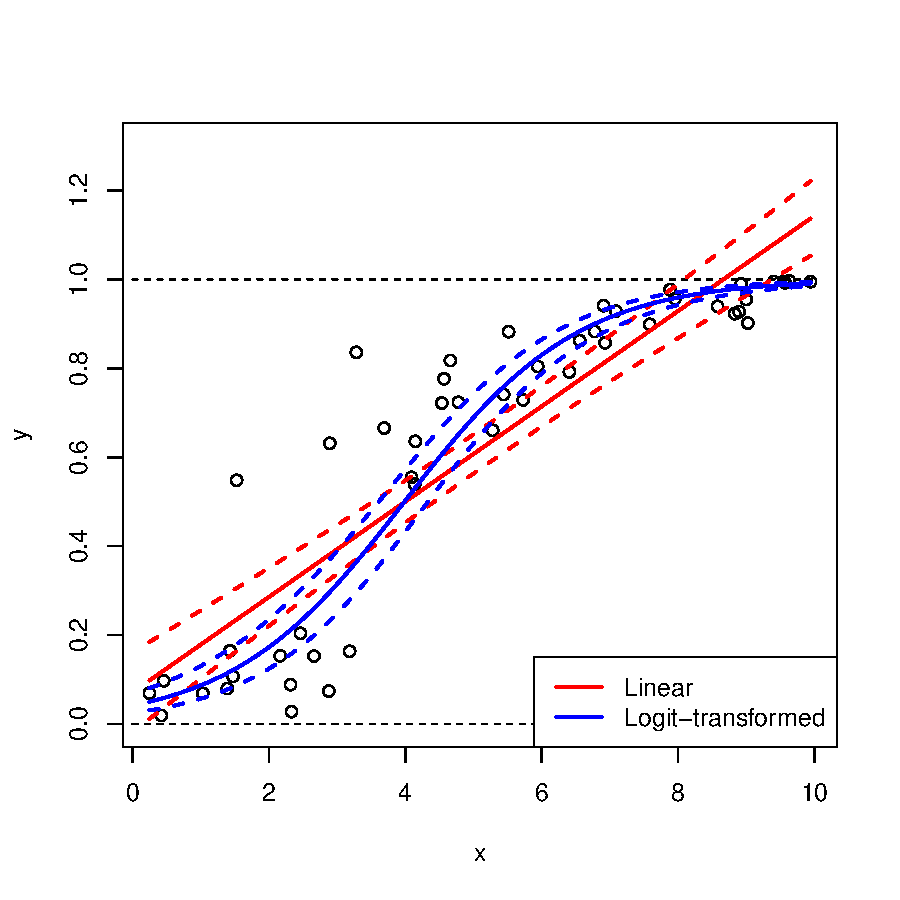
\includegraphics[keepaspectratio]{chapters/ch11_files/figure-pdf/unnamed-chunk-18-1.pdf}}
\end{center}

The downside of the logit transform is that it is undefined at at 0 and
1 (it approaches \(-\infty\) and \(+\infty\) as the inputs approach 0
and 1). One workaround is to add a small constant to avoid taking
\(\log{\left(0\right)}\) or dividing by 0 (McCune \emph{et al.} 2002;
Warton and Hui 2011). The latter reference suggests adding the minimum
non-zero value. You could also censor the values to be arbitrarily close
to 0 or 1: for example, set all values \(<0.001\) to 0.001 and all
values \(>0.999\) to 0.999. This practice is sometimes called
``stabilizing the logit'' (Kéry 2010).

\begin{Shaded}
\begin{Highlighting}[]
\CommentTok{\# change some values in y to 1 and 0}
\NormalTok{y[}\FunctionTok{which.max}\NormalTok{(y)] }\OtherTok{\textless{}{-}} \DecValTok{1}
\NormalTok{y[}\FunctionTok{which.min}\NormalTok{(y)] }\OtherTok{\textless{}{-}} \DecValTok{0}

\CommentTok{\# logit transformed values include infinities!}
\FunctionTok{qlogis}\NormalTok{(y)}
\end{Highlighting}
\end{Shaded}

\begin{verbatim}
 [1] -2.5298619  3.7500756  0.2207000  2.4844936  5.3073196 -2.2318620
 [7]  0.6657197  4.5882685  2.0138961  1.2461916  4.8648903  0.9539238
[13]  2.0198681  0.9887879 -2.6085359  3.0539803 -1.3622593       -Inf
[19]  1.6283614  5.3667394  2.5484363  1.7931407  1.3371457  5.2369884
[25]  1.8344244  2.5672970  1.0519484  1.4131947  0.5373003 -2.1224186
[31]        Inf  2.2184900  2.7649033  3.0898599 -2.5994558  0.9631093
[37]  2.1861231 -1.7101479 -1.6322178 -2.3345978 -1.6254712  0.5573073
[43]  0.1559367  0.6886083  0.1934203 -2.4499857 -3.5614131  1.5004569
[49] -1.7144060  2.7456992
\end{verbatim}

\begin{Shaded}
\begin{Highlighting}[]
\CommentTok{\# stabilize logit by setting max to 0.999 and min to 0.001}
\NormalTok{y }\OtherTok{\textless{}{-}} \FunctionTok{pmin}\NormalTok{(}\FloatTok{0.999}\NormalTok{, y)}
\NormalTok{y }\OtherTok{\textless{}{-}} \FunctionTok{pmax}\NormalTok{(}\FloatTok{0.001}\NormalTok{, y)}
\FunctionTok{qlogis}\NormalTok{(y)}
\end{Highlighting}
\end{Shaded}

\begin{verbatim}
 [1] -2.5298619  3.7500756  0.2207000  2.4844936  5.3073196 -2.2318620
 [7]  0.6657197  4.5882685  2.0138961  1.2461916  4.8648903  0.9539238
[13]  2.0198681  0.9887879 -2.6085359  3.0539803 -1.3622593 -6.9067548
[19]  1.6283614  5.3667394  2.5484363  1.7931407  1.3371457  5.2369884
[25]  1.8344244  2.5672970  1.0519484  1.4131947  0.5373003 -2.1224186
[31]  6.9067548  2.2184900  2.7649033  3.0898599 -2.5994558  0.9631093
[37]  2.1861231 -1.7101479 -1.6322178 -2.3345978 -1.6254712  0.5573073
[43]  0.1559367  0.6886083  0.1934203 -2.4499857 -3.5614131  1.5004569
[49] -1.7144060  2.7456992
\end{verbatim}

\subsubsection{Probit transformation}\label{sec-trans-common-lp-probit}

Like the logit function, the probit function maps probabilities to the
real number line. However, the probit function uses the CDF of the
standard normal distribution instead of the logit function. The logit
and the probit can be used in many of the same situations. Whereas the
logit maps a probability using the log-odds, the probit maps a
probability to the corresponding quantile of the standard normal
distribution:

\[probit\left(x\right)=\Phi^{-1}\left(x\right)\] where \(\Phi\) is the
CDF of the standard normal distribution (i.e.,
\(Normal\left(\mu=1,\sigma=1\right)\)). For example, a probability of
0.5 corresponds to a probit of 0, while probabilities of 0.025, and
0.975 correspond to probits of -1.96 and +1.96.

The R command for the probit function is \texttt{qnorm()}. As you might
suspect from \href{@sec-dist-norm-r}{the previous module}, the inverse
function is \texttt{pnorm()}.

\begin{Shaded}
\begin{Highlighting}[]
\NormalTok{x }\OtherTok{\textless{}{-}} \DecValTok{1}\SpecialCharTok{:}\DecValTok{99}\SpecialCharTok{/}\DecValTok{100}
\NormalTok{x.log }\OtherTok{\textless{}{-}} \FunctionTok{qlogis}\NormalTok{(x)}
\NormalTok{x.prb }\OtherTok{\textless{}{-}} \FunctionTok{qnorm}\NormalTok{(x)}

\FunctionTok{plot}\NormalTok{(x, x.log, }\AttributeTok{type=}\StringTok{"l"}\NormalTok{,}
    \AttributeTok{lwd=}\DecValTok{3}\NormalTok{, }\AttributeTok{xlab=}\StringTok{"x"}\NormalTok{, }\AttributeTok{ylab=}\StringTok{"f(x)"}\NormalTok{)}
\FunctionTok{points}\NormalTok{(x, x.prb, }\AttributeTok{type=}\StringTok{"l"}\NormalTok{, }\AttributeTok{lwd=}\DecValTok{3}\NormalTok{,}
    \AttributeTok{col=}\StringTok{"red"}\NormalTok{, }\AttributeTok{lty=}\DecValTok{2}\NormalTok{)}
\FunctionTok{abline}\NormalTok{(}\AttributeTok{h=}\DecValTok{0}\NormalTok{, }\AttributeTok{lty=}\DecValTok{3}\NormalTok{, }\AttributeTok{col=}\StringTok{"blue"}\NormalTok{)}
\FunctionTok{abline}\NormalTok{(}\AttributeTok{v=}\FloatTok{0.5}\NormalTok{, }\AttributeTok{lty=}\DecValTok{3}\NormalTok{, }\AttributeTok{col=}\StringTok{"blue"}\NormalTok{)}
\FunctionTok{legend}\NormalTok{(}\StringTok{"topleft"}\NormalTok{,}
    \AttributeTok{legend=}\FunctionTok{c}\NormalTok{(}\StringTok{"Logit(x)"}\NormalTok{, }\StringTok{"Probit(x)"}\NormalTok{),}
    \AttributeTok{lwd=}\DecValTok{3}\NormalTok{, }\AttributeTok{col=}\FunctionTok{c}\NormalTok{(}\StringTok{"black"}\NormalTok{, }\StringTok{"red"}\NormalTok{), }\AttributeTok{lty=}\DecValTok{1}\SpecialCharTok{:}\DecValTok{2}\NormalTok{)}
\end{Highlighting}
\end{Shaded}

\begin{center}
\pandocbounded{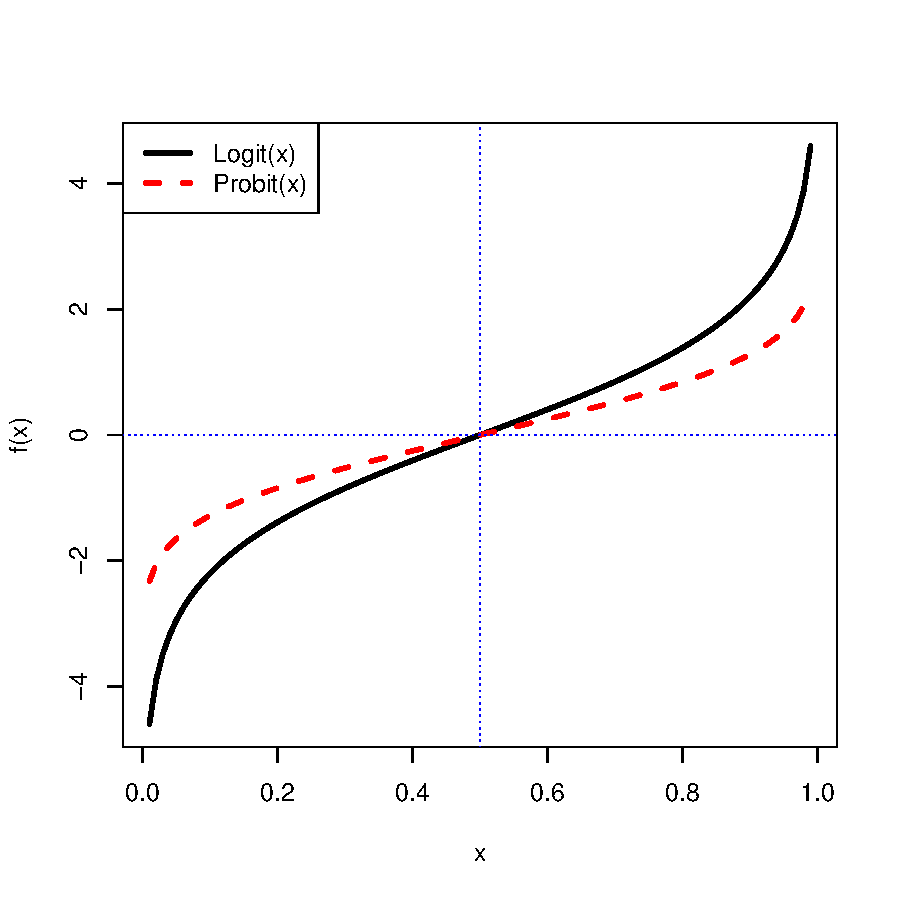
\includegraphics[keepaspectratio]{chapters/ch11_files/figure-pdf/chunkx460-1.pdf}}
\end{center}

The figure above shows a logit and probit transform of probabilities
from 0.01 to 0.99. The blue dashed lines show that both functions map
\(p=0.05\) to 0. The logit and probit functions are similar near the
center of the probability range but differ increasingly near 0 and 1.
The logit approaches \(\pm\infty\) more rapidly because the
corresponding logistic distribution has heavier tails than the normal
distribution. Despite this difference, logit and probit GLMs usually
produce very similar fitted probabilities except when probabilities are
extreme.

In practice, logit and probit links or transforms usually produce very
similar fitted probabilities, and the choice between them often has
little effect on the biological conclusions. The logit is particularly
convenient because its coefficients can be interpreted using odds ratios
(see Section~\ref{sec-glm4-logistics-or}). The probit can be useful when
there is a reason to imagine an underlying normally distributed
continuous variable that produces a binary outcome when it crosses a
threshold. For example, an organism might die when an unobserved
physiological stress exceeds some threshold, or an animal might choose
one habitat when an underlying preference exceeds a threshold. This
latent-variable interpretation is one reason probit models are used in
some fields.

Probit models have historically been especially common in toxicology and
dose-response studies. If individuals differ in their tolerance to a
toxin and those tolerances are approximately normally distributed, the
proportion responding at a given dose can be modeled using the normal
CDF. This approach was historically known as probit analysis and has
been widely used to estimate quantities such as LD50.

\section{Uncommon transformations}\label{sec-trans-uncommon}

\subsection{Square-root transformation}\label{sec-trans-uncommon-sqrt}

\textbf{Square-root transforms} map values to their square roots. This
is sometimes used as a variance-stabilizing transformation, similar to
the log transform. Square-root transforms are useful when a response
variable is proportional to the square of the explanatory variable, or
when the data show heteroscedasticity (non-constant variance). Counts
are sometimes analyzed using a square-root transform. The square-root
transform is a special case of the \textbf{power transform} (where
values are raised to a power) and a special case of the Box-Cox
transform (see Section~\ref{sec-trans-uncommon-boxcox}). The square-root
function in R is \texttt{sqrt()}. There are several ways to accomplish a
square-root transform in R:

\begin{Shaded}
\begin{Highlighting}[]
\NormalTok{x }\OtherTok{\textless{}{-}} \FunctionTok{rnorm}\NormalTok{(}\DecValTok{20}\NormalTok{, }\DecValTok{5}\NormalTok{, }\DecValTok{1}\NormalTok{)}
\NormalTok{y }\OtherTok{\textless{}{-}} \FunctionTok{sqrt}\NormalTok{(x)}
\NormalTok{z }\OtherTok{\textless{}{-}}\NormalTok{ x}\SpecialCharTok{\^{}}\FloatTok{0.5}
\end{Highlighting}
\end{Shaded}

Higher roots (cube root, fourth root, etc.) are sometimes used as
transforms, but this is not very common.

\begin{Shaded}
\begin{Highlighting}[]
\NormalTok{w }\OtherTok{\textless{}{-}}\NormalTok{ x}\SpecialCharTok{\^{}}\NormalTok{(}\DecValTok{1}\SpecialCharTok{/}\DecValTok{3}\NormalTok{) }\CommentTok{\# cube root}
\end{Highlighting}
\end{Shaded}

Here is an example of using the square root transform on right-skewed
data:

\begin{Shaded}
\begin{Highlighting}[]
\FunctionTok{set.seed}\NormalTok{(}\DecValTok{123}\NormalTok{)}
\NormalTok{x }\OtherTok{\textless{}{-}} \FunctionTok{rlnorm}\NormalTok{(}\DecValTok{100}\NormalTok{, }\DecValTok{2}\NormalTok{, }\DecValTok{1}\NormalTok{)}
\FunctionTok{par}\NormalTok{(}\AttributeTok{mfrow=}\FunctionTok{c}\NormalTok{(}\DecValTok{1}\NormalTok{,}\DecValTok{3}\NormalTok{), }\AttributeTok{cex.lab=}\FloatTok{1.4}\NormalTok{)}
\FunctionTok{hist}\NormalTok{(x, }\AttributeTok{main=}\StringTok{"Original values"}\NormalTok{)}
\FunctionTok{hist}\NormalTok{(}\FunctionTok{sqrt}\NormalTok{(x), }\AttributeTok{main=}\StringTok{"Square root transform"}\NormalTok{, }\AttributeTok{xlab=}\FunctionTok{expression}\NormalTok{(}\FunctionTok{sqrt}\NormalTok{(x)))}
\FunctionTok{hist}\NormalTok{(x}\SpecialCharTok{\^{}}\NormalTok{(}\DecValTok{1}\SpecialCharTok{/}\DecValTok{3}\NormalTok{), }\AttributeTok{main=}\StringTok{"Cube root transform"}\NormalTok{, }\AttributeTok{xlab=}\FunctionTok{expression}\NormalTok{(}\FunctionTok{root}\NormalTok{(x,}\DecValTok{3}\NormalTok{)))}
\end{Highlighting}
\end{Shaded}

\pandocbounded{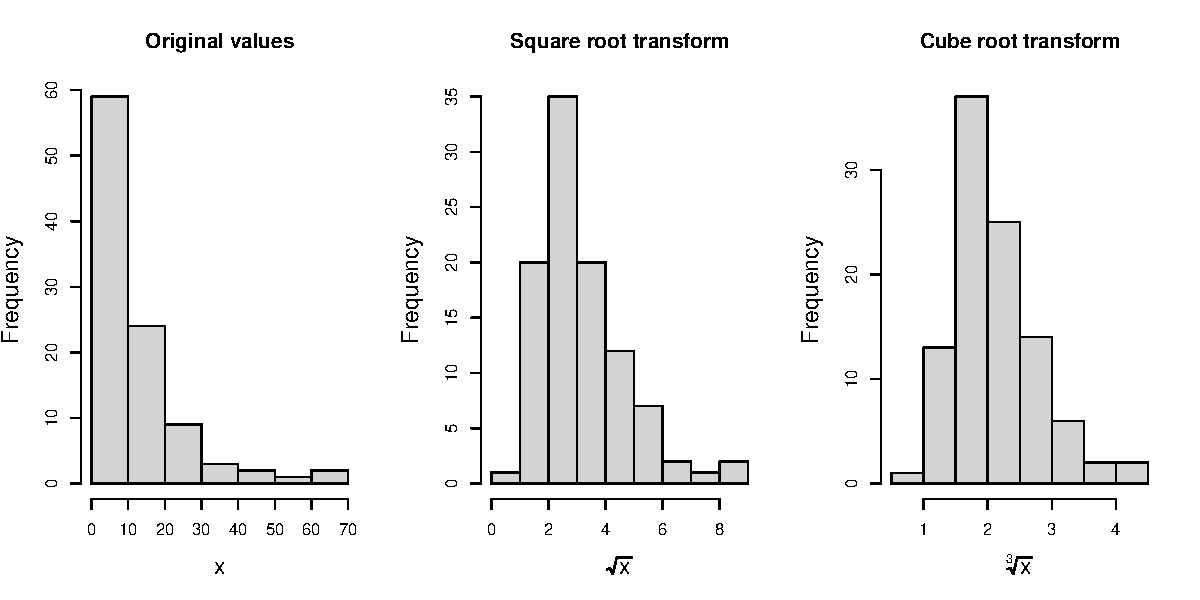
\includegraphics[keepaspectratio]{chapters/ch11_files/figure-pdf/unnamed-chunk-23-1.pdf}}

Notice how the square- and cube-root transformed data appear much more
normally-distributed than the original data.

\begin{Shaded}
\begin{Highlighting}[]
\CommentTok{\# reset plot layout}
\FunctionTok{par}\NormalTok{(}\AttributeTok{mfrow=}\FunctionTok{c}\NormalTok{(}\DecValTok{1}\NormalTok{,}\DecValTok{1}\NormalTok{))}
\end{Highlighting}
\end{Shaded}

\subsection{Arcsine square root
transformation}\label{sec-trans-uncommon-asin}

Another transformation historically used for proportional data is to use
the \textbf{arcsine square root transform}, or \textbf{arcsine
transform} for short:

\[y_i=\frac{2}{\pi}arcsin\left(\sqrt{x_i}\right)\]

Some sources omit the coefficient \(2/\pi\); others do not. Including
the \(2/\pi\) rescales the function so that the transformed values range
from 0 to 1 (McCune \emph{et al.} 2002). Without this factor, the
function maps probabilities to \(\left[0,\pi/2\right]\) instead of
\(\left[0,1\right]\).

For a binomial proportion, variance depends on the underlying
probability \(p\), with proportions near 0 or 1 having different
variance than those near 0.5. The arcsine transform was used as a
variance-stabilizing transformation to reduce the dependence of the
variance on the mean.

Although historically common in biology, the arcsine square-root
transform is generally not recommended when proportions arise from an
identifiable binomial process. A binomial GLM
(Section~\ref{sec-glm4-binom}) models the mean-variance relationship
directly while respecting the bounded nature of the response, and is
usually preferable to transforming the proportions. The transformation
has also been criticized for ecological proportional data more generally
(Warton and Hui 2011). Thus, its main importance today may be in
understanding older literature rather than as a default method for
analyzing new data.

If you insist on using the arcsine transform, you can do it in R using
\texttt{asin()} function. In the examples below, \texttt{asin()} is
embedded inside custom functions that perform the other parts of the
arcsine transform.

\begin{Shaded}
\begin{Highlighting}[]
\CommentTok{\# unscaled version:}
\NormalTok{asin.trans1 }\OtherTok{\textless{}{-}} \ControlFlowTok{function}\NormalTok{(p) \{}\FunctionTok{asin}\NormalTok{(}\FunctionTok{sqrt}\NormalTok{(p))\}}

\CommentTok{\# scaled version:}
\NormalTok{asin.trans2 }\OtherTok{\textless{}{-}} \ControlFlowTok{function}\NormalTok{(p) \{}\DecValTok{2}\SpecialCharTok{/}\NormalTok{pi}\SpecialCharTok{*}\FunctionTok{asin}\NormalTok{(}\FunctionTok{sqrt}\NormalTok{(p))\}}

\CommentTok{\# example of use}
\NormalTok{x }\OtherTok{\textless{}{-}} \FunctionTok{seq}\NormalTok{(}\FloatTok{0.001}\NormalTok{, }\FloatTok{0.999}\NormalTok{, }\AttributeTok{by=}\FloatTok{0.001}\NormalTok{)}
\NormalTok{y1 }\OtherTok{\textless{}{-}} \FunctionTok{asin.trans1}\NormalTok{(x)}
\NormalTok{y2 }\OtherTok{\textless{}{-}} \FunctionTok{asin.trans2}\NormalTok{(x)}

\CommentTok{\# compare with and without 2/pi coefficient:}
\FunctionTok{plot}\NormalTok{(x,y1, }\AttributeTok{ylim=}\FunctionTok{c}\NormalTok{(}\DecValTok{0}\NormalTok{, }\FloatTok{1.6}\NormalTok{), }\AttributeTok{type=}\StringTok{"l"}\NormalTok{, }\AttributeTok{lwd=}\DecValTok{3}\NormalTok{)}
\FunctionTok{points}\NormalTok{(x, y2, }\AttributeTok{col=}\StringTok{"red"}\NormalTok{, }\AttributeTok{type=}\StringTok{"l"}\NormalTok{, }\AttributeTok{lwd=}\DecValTok{3}\NormalTok{, }\AttributeTok{lty=}\DecValTok{2}\NormalTok{)}
\FunctionTok{legend}\NormalTok{(}\StringTok{"topleft"}\NormalTok{,}
       \AttributeTok{legend=}\FunctionTok{c}\NormalTok{(}\StringTok{"Unscaled version"}\NormalTok{, }\StringTok{"Scaled version"}\NormalTok{),}
       \AttributeTok{lwd=}\DecValTok{3}\NormalTok{, }\AttributeTok{lty=}\DecValTok{1}\SpecialCharTok{:}\DecValTok{2}\NormalTok{, }\AttributeTok{col=}\FunctionTok{c}\NormalTok{(}\StringTok{"black"}\NormalTok{, }\StringTok{"red"}\NormalTok{), }
       \AttributeTok{cex=}\FloatTok{1.4}\NormalTok{)}
\end{Highlighting}
\end{Shaded}

\begin{center}
\pandocbounded{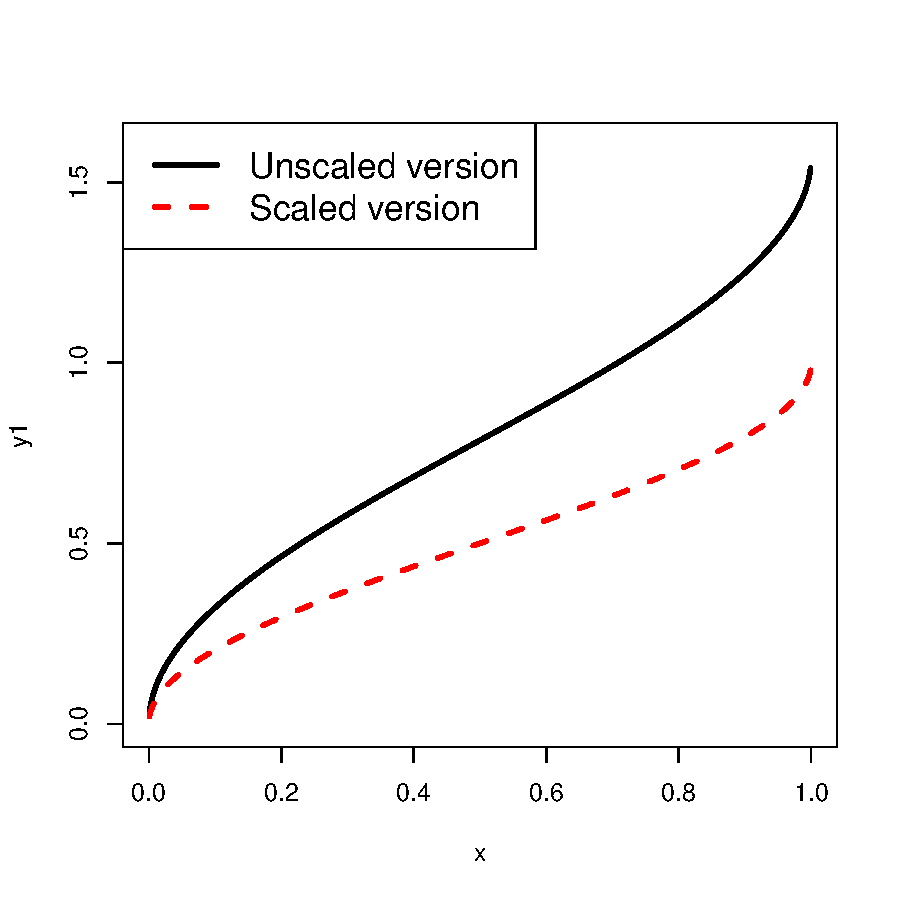
\includegraphics[keepaspectratio]{chapters/ch11_files/figure-pdf/unnamed-chunk-25-1.pdf}}
\end{center}

The plot below compares the arcsine to the logit transformation for
proportional data.

\begin{Shaded}
\begin{Highlighting}[]
\CommentTok{\# compare to logit transform:}
\NormalTok{y3 }\OtherTok{\textless{}{-}} \FunctionTok{qlogis}\NormalTok{(x)}
\FunctionTok{plot}\NormalTok{(x,y1, }\AttributeTok{ylim=}\FunctionTok{c}\NormalTok{(}\SpecialCharTok{{-}}\DecValTok{5}\NormalTok{, }\DecValTok{5}\NormalTok{), }\AttributeTok{xlim=}\FunctionTok{c}\NormalTok{(}\DecValTok{0}\NormalTok{,}\DecValTok{1}\NormalTok{), }\AttributeTok{type=}\StringTok{"l"}\NormalTok{)}
\FunctionTok{points}\NormalTok{(x, y2, }\AttributeTok{col=}\StringTok{"red"}\NormalTok{, }\AttributeTok{type=}\StringTok{"l"}\NormalTok{, }\AttributeTok{lwd=}\DecValTok{3}\NormalTok{, }\AttributeTok{lty=}\DecValTok{2}\NormalTok{)}
\FunctionTok{points}\NormalTok{(x, y3, }\AttributeTok{col=}\StringTok{"blue"}\NormalTok{, }\AttributeTok{type=}\StringTok{"l"}\NormalTok{, }\AttributeTok{lwd=}\DecValTok{3}\NormalTok{, }\AttributeTok{lty=}\DecValTok{3}\NormalTok{)}
\FunctionTok{legend}\NormalTok{(}\StringTok{"topleft"}\NormalTok{, }
       \AttributeTok{legend=}\FunctionTok{c}\NormalTok{(}\StringTok{"Unscaled arcsine"}\NormalTok{,}
                \StringTok{"Scaled arcsine"}\NormalTok{,}
                \StringTok{"Logit"}\NormalTok{),}
       \AttributeTok{lty=}\DecValTok{1}\SpecialCharTok{:}\DecValTok{3}\NormalTok{, }\AttributeTok{lwd=}\DecValTok{3}\NormalTok{, }\AttributeTok{col=}\FunctionTok{c}\NormalTok{(}\StringTok{"black"}\NormalTok{, }\StringTok{"red"}\NormalTok{, }\StringTok{"blue"}\NormalTok{), }\AttributeTok{cex=}\FloatTok{1.4}\NormalTok{)}
\end{Highlighting}
\end{Shaded}

\begin{center}
\pandocbounded{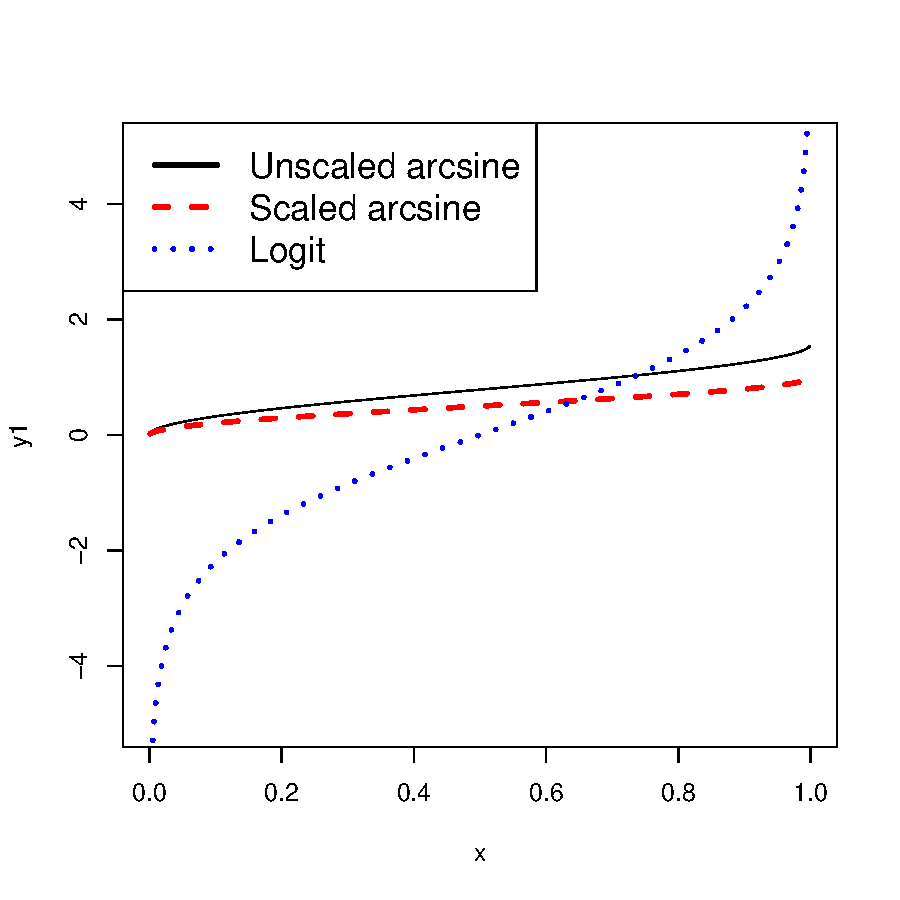
\includegraphics[keepaspectratio]{chapters/ch11_files/figure-pdf/unnamed-chunk-26-1.pdf}}
\end{center}

Unlike the logit, the arcsine transform remains bounded at \(p=0\) and
\(p=1\). Consequently, it can transform observed proportions of exactly
0 or 1 without adjustment, whereas logit is undefined at those values.

\subsection{Box-Cox transformation}\label{sec-trans-uncommon-boxcox}

The Box-Cox transformation is a family of power transformations used to
identify a useful transformation of a positive response variable in a
statistical model (Box and Cox 1964). Rather than choosing a
transformation such as square root or logarithm by hand, the Box-Cox
procedure estimates a parameter \(\lambda\) that determines the
transformation.

\[
y_i^{(\lambda)}=
\begin{cases}
\log(y_i), & \lambda=0 \\[4pt]
\dfrac{y_i^\lambda-1}{\lambda}, & \lambda\ne0
\end{cases}
\]

Thus, Box-Cox includes many familiar transformations as special cases. A
value of \(\lambda=1\) corresponds essentially to no transformation,
\(\lambda=0.5\) to a square-root transformation, \(\lambda=0\) to a
logarithmic transformation, and \(\lambda=-1\) to a reciprocal
transformation.

\begin{longtable}[]{@{}rl@{}}
\caption{Common values of \(\lambda\) and their approximate
corresponding transformations in the Box-Cox
family.}\label{tbl-boxcox-transform}\tabularnewline
\toprule\noalign{}
\(\lambda\) & Approximate transformation \\
\midrule\noalign{}
\endfirsthead
\toprule\noalign{}
\(\lambda\) & Approximate transformation \\
\midrule\noalign{}
\endhead
\bottomrule\noalign{}
\endlastfoot
\(2\) & \(y^2\) \\
\(1\) & \(y\) (no transformation) \\
\(0.5\) & \(\sqrt{y}\) \\
\(0\) & \(\log(y)\) \\
\(-0.5\) & \(1/\sqrt{y}\) \\
\(-1\) & \(1/y\) \\
\end{longtable}

Here the parameter \(\lambda\) is some constant that must be optimized
for a given variable. When \(\lambda=0\), the transformation is defined
as \(y_i=\log{\left(x_i\right)}\).

Unlike the transformations considered above, Box-Cox is usually applied
in the context of a statistical model. A model is fitted repeatedly
using different values of \(\lambda\), and the likelihood is calculated
for each. The value of \(\lambda\) that maximizes the likelihood is the
estimated optimal transformation.

The Box-Cox transformation is available in several packages, but not
base R. Here is an example using the functions in package MASS:

\begin{Shaded}
\begin{Highlighting}[]
\FunctionTok{set.seed}\NormalTok{(}\DecValTok{123}\NormalTok{)}

\NormalTok{n }\OtherTok{\textless{}{-}} \DecValTok{100}
\NormalTok{x }\OtherTok{\textless{}{-}} \FunctionTok{runif}\NormalTok{(n, }\DecValTok{0}\NormalTok{, }\DecValTok{5}\NormalTok{)}

\CommentTok{\# relationship is linear with normal errors on log scale}
\NormalTok{logy }\OtherTok{\textless{}{-}} \DecValTok{1} \SpecialCharTok{+} \FloatTok{0.4}\SpecialCharTok{*}\NormalTok{x }\SpecialCharTok{+} \FunctionTok{rnorm}\NormalTok{(n, }\DecValTok{0}\NormalTok{, }\FloatTok{0.3}\NormalTok{)}
\NormalTok{y }\OtherTok{\textless{}{-}} \FunctionTok{exp}\NormalTok{(logy)}

\CommentTok{\# but on linear scale, relationship appears nonlinear}
\FunctionTok{plot}\NormalTok{(x, y, }\AttributeTok{pch=}\DecValTok{16}\NormalTok{)}
\end{Highlighting}
\end{Shaded}

\begin{center}
\pandocbounded{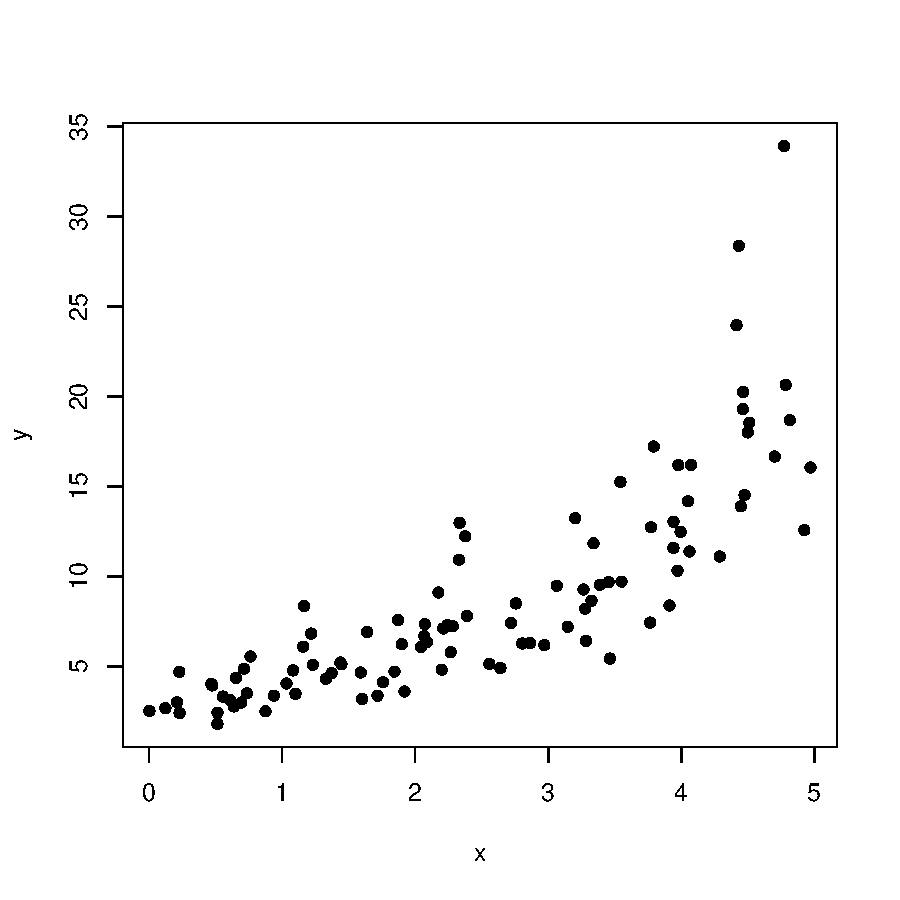
\includegraphics[keepaspectratio]{chapters/ch11_files/figure-pdf/unnamed-chunk-27-1.pdf}}
\end{center}

\begin{Shaded}
\begin{Highlighting}[]
\CommentTok{\# fit a linear model}
\NormalTok{m1 }\OtherTok{\textless{}{-}} \FunctionTok{lm}\NormalTok{(y }\SpecialCharTok{\textasciitilde{}}\NormalTok{ x)}

\CommentTok{\# some model diagnostics}
\FunctionTok{par}\NormalTok{(}\AttributeTok{mfrow=}\FunctionTok{c}\NormalTok{(}\DecValTok{1}\NormalTok{,}\DecValTok{2}\NormalTok{))}
\FunctionTok{plot}\NormalTok{(m1, }\AttributeTok{which=}\DecValTok{1}\NormalTok{)}
\FunctionTok{plot}\NormalTok{(m1, }\AttributeTok{which=}\DecValTok{2}\NormalTok{)}
\end{Highlighting}
\end{Shaded}

\pandocbounded{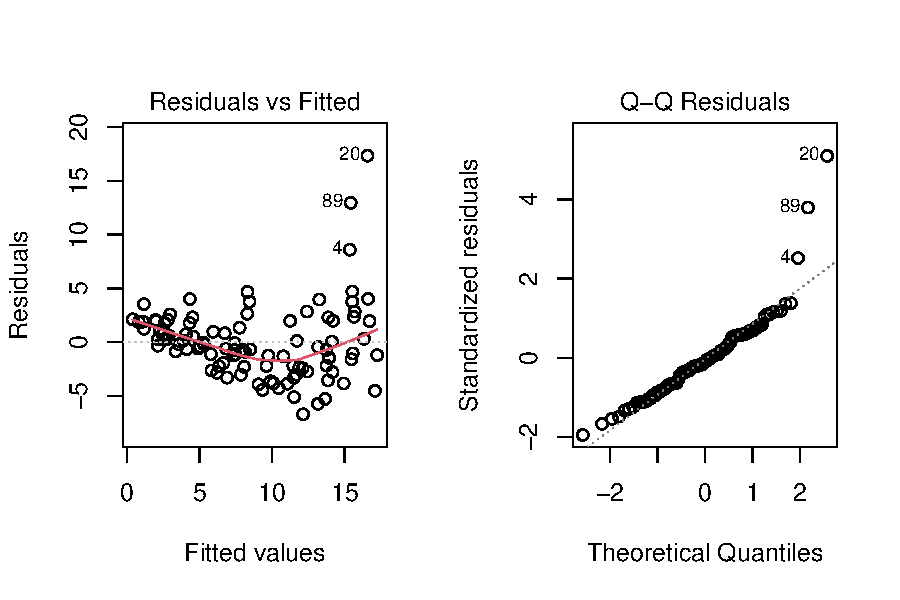
\includegraphics[keepaspectratio]{chapters/ch11_files/figure-pdf/unnamed-chunk-28-1.pdf}}

Notice how the diagnostic plots show some patterns in the residuals,
violating the assumptions of the linear regression model. A Box-Cox
transformation might help here.

\begin{Shaded}
\begin{Highlighting}[]
\FunctionTok{library}\NormalTok{(MASS)}

\NormalTok{bc }\OtherTok{\textless{}{-}} \FunctionTok{boxcox}\NormalTok{(m1)}
\end{Highlighting}
\end{Shaded}

\pandocbounded{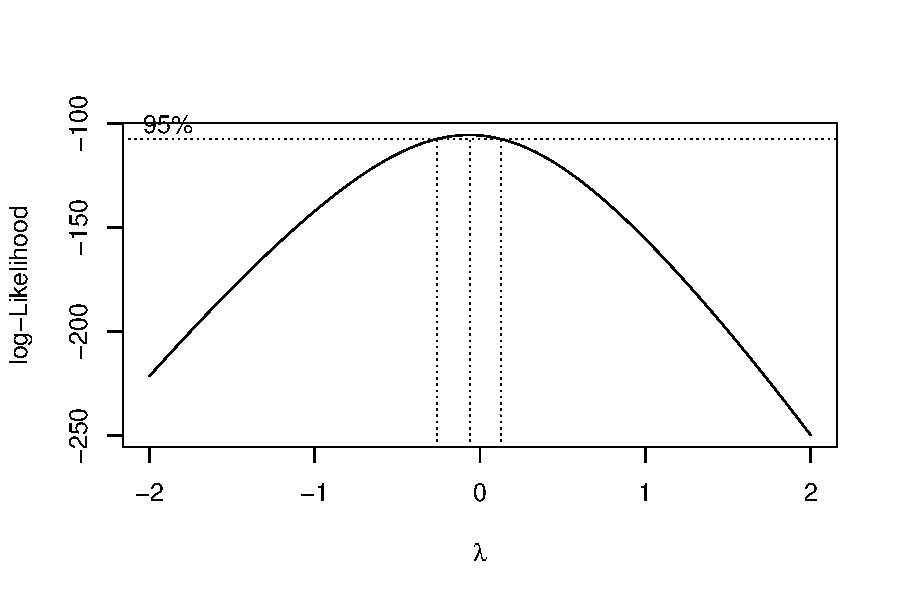
\includegraphics[keepaspectratio]{chapters/ch11_files/figure-pdf/unnamed-chunk-29-1.pdf}}

The Box-Cox function estimated an optimal \(\lambda\) near 0, which
corresponds to the log transformation that actually generated the data
(see Table~\ref{tbl-boxcox-transform}).

Then, we extract the optimal \(\lambda\):

\begin{Shaded}
\begin{Highlighting}[]
\NormalTok{use.lambda }\OtherTok{\textless{}{-}}\NormalTok{ bc}\SpecialCharTok{$}\NormalTok{x[}\FunctionTok{which.max}\NormalTok{(bc}\SpecialCharTok{$}\NormalTok{y)]}
\NormalTok{use.lambda}
\end{Highlighting}
\end{Shaded}

\begin{verbatim}
[1] -0.06060606
\end{verbatim}

You don't need to use the estimated value blindly. In this case, it is
close to 0, suggesting a log transform ().

\begin{Shaded}
\begin{Highlighting}[]
\CommentTok{\# refit the model with the log transform}
\NormalTok{m2 }\OtherTok{\textless{}{-}} \FunctionTok{lm}\NormalTok{(}\FunctionTok{log}\NormalTok{(y) }\SpecialCharTok{\textasciitilde{}}\NormalTok{ x)}

\CommentTok{\# compare diagnostic plots}
\FunctionTok{par}\NormalTok{(}\AttributeTok{mfrow=}\FunctionTok{c}\NormalTok{(}\DecValTok{2}\NormalTok{,}\DecValTok{2}\NormalTok{), }\AttributeTok{mar=}\FunctionTok{c}\NormalTok{(}\FloatTok{5.1}\NormalTok{, }\FloatTok{5.1}\NormalTok{, }\FloatTok{2.1}\NormalTok{, }\FloatTok{1.1}\NormalTok{))}
\FunctionTok{plot}\NormalTok{(m1, }\AttributeTok{which=}\DecValTok{1}\NormalTok{)}
\FunctionTok{plot}\NormalTok{(m1, }\AttributeTok{which=}\DecValTok{2}\NormalTok{)}
\FunctionTok{plot}\NormalTok{(m2, }\AttributeTok{which=}\DecValTok{1}\NormalTok{)}
\FunctionTok{plot}\NormalTok{(m2, }\AttributeTok{which=}\DecValTok{2}\NormalTok{)}
\end{Highlighting}
\end{Shaded}

\pandocbounded{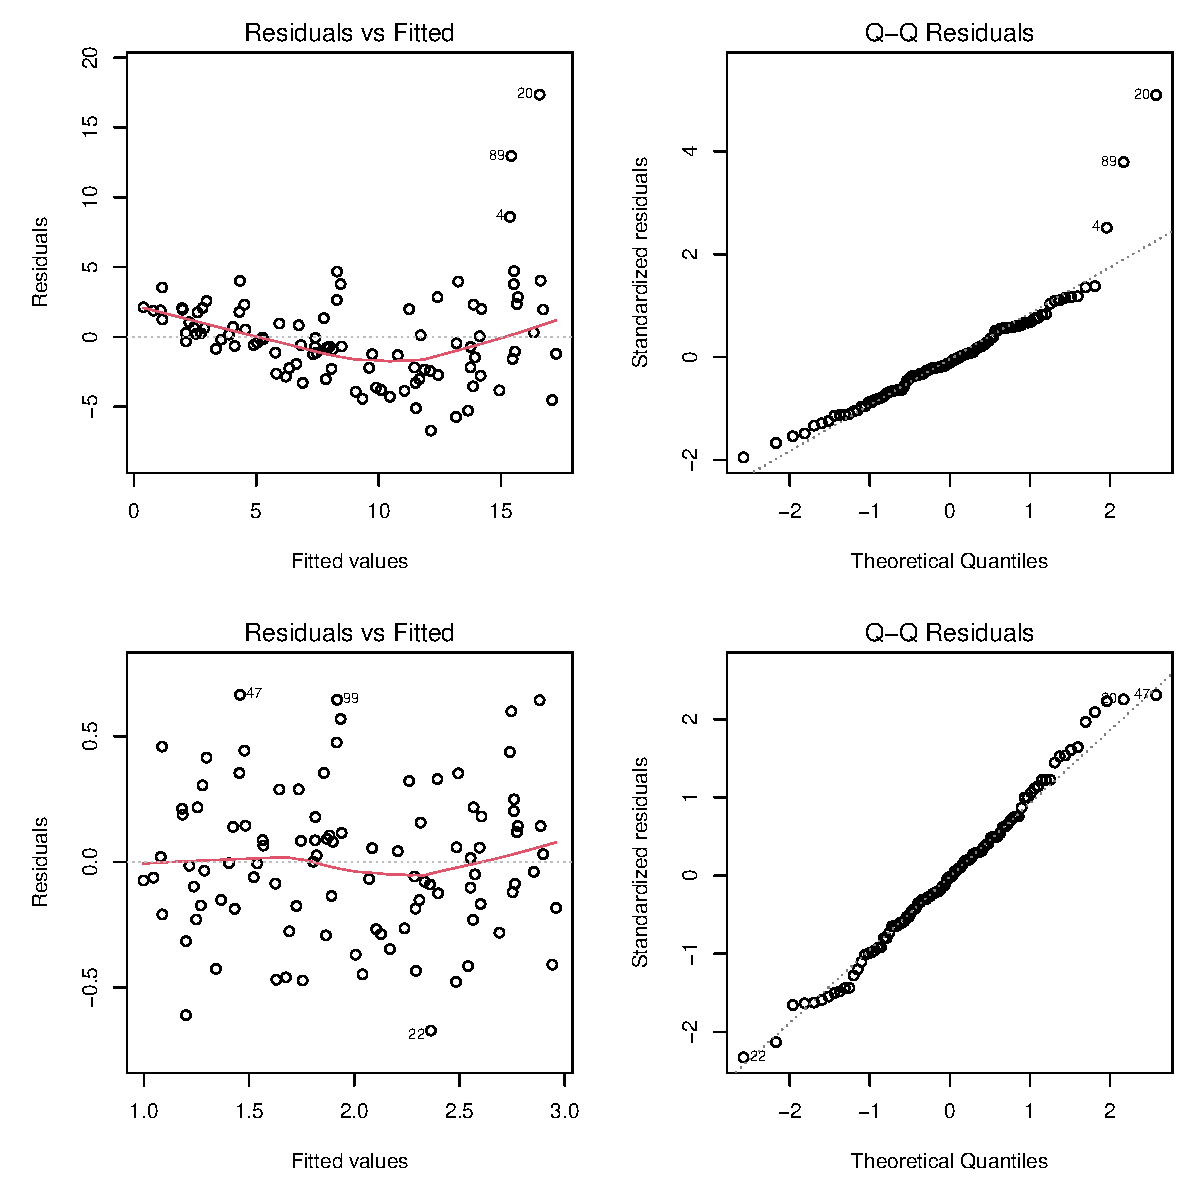
\includegraphics[keepaspectratio]{chapters/ch11_files/figure-pdf/unnamed-chunk-31-1.pdf}}

The Box-Cox transformation requires positive response values. In
practice, its estimated value of \(\lambda\) is often most useful as a
guide to choosing a simple, interpretable transformation rather than as
a requirement to use the exact estimated value. As with any
transformation, its success should ultimately be evaluated by examining
the fitted model and its diagnostic plots.

The Box-Cox procedure was developed when transforming data to satisfy
the assumptions of linear models was a common solution to non-normality,
nonlinearity, and non-constant variance. It remains useful for
identifying appropriate power transformations, but many problems that
once motivated Box-Cox transformations can now be addressed more
directly using generalized linear models or other models that explicitly
represent the distribution and mean-variance relationship of the
response.

\section{Transformations closing thoughts}\label{sec-trans-close}

A transformation should not be chosen simply because it makes a
scatterplot look more linear or a histogram look more normal. Before
transforming a variable, consider \textbf{why} the observed pattern has
its shape. A curved relationship may arise because the variables are
related on a multiplicative scale, in which case a transformation may be
useful. It may instead reflect the mean-variance relationship or support
of a particular probability distribution, which may be better handled
using a GLM. Alternatively, the curvature may reflect a genuinely
nonlinear biological process, in which case a nonlinear model may
provide a more meaningful description. The goal is not to make the data
fit the model; it is to choose a model and scale that appropriately
represent the data and the biological process that generated them.

\chapter{Common problems in biological data}\label{sec-problems}

Many statistical methods assume that data follow certain distributions,
and we have already explored methods for making sure your data follow
those distributions. Other problems are not so easy to diagnose or fix.
This section will introduce you to some methods for dealing with more
subtle data problems. Note that none of these issues have
one-size-fits-all solutions. Dealing with these issues will require
understanding your study system and thinking through the consequences of
potential solutions.

\section{Outliers and erroneous
values}\label{outliers-and-erroneous-values}

Outliers are values that much larger or smaller than other values in the
data set. While these values are theoretically possible in any
distribution, they are by their nature extremely unlikely. Outliers can
cause problems with many statistical tests because they are often given
undue weight. This is because deviations from the mean are often
squared.

There are two problems with outliers: how to detect them, and what to do
with them.

\subsection{Detecting outliers}\label{detecting-outliers}

There are several definitions of outlier. Some researchers have
suggested simple measures such as \emph{Z}-scores to detect outliers.
\emph{Z}-scores measure how many standard deviations (SD) an observation
is away from the mean. The \emph{Z}-score of an observation \(x_i\)
(observation \emph{i} of variable \emph{x}) is calculated as:

\[Z\left(x_i\right)=\frac{x_i-\bar{x}}{\sigma\left(x\right)}\]

where \(\bar{x}\) is the mean of \emph{x} and \(\sigma\left(x\right)\)
is the SD of \emph{x}. For example, \emph{Z}-scores of -2.3 and +4.1
indicate observations 2.3 SD below and 4.1 SD above the mean,
respectively. \emph{Z}-scores are also referred to as \textbf{sigmas},
referring to the symbol for SD. E.g., a 4\(\sigma\) observation is 4 SD
away from the mean. Various \(\sigma\) levels have been used to detect
outliers, in which researchers discard any observation 2\(\sigma\),
3\(\sigma\), etc., away from the mean. This threshold varies by
discipline, so follow the conventions in your field.

The figure below shows \emph{Z}-scores relative to the standard normal
distribution (\(\mu\) = 0, SD = 1). About 68\% of observations are
expected to have a \emph{Z}-score between -1 and 1--i.e., deviate by
\(\le\) 1 \(\sigma\). About 95\% of observations should be \(\le\) 2
\(\sigma\), and over 99\% of observations should be \(\le\) 3
\(\sigma\). The greater the magnitude of a value's \emph{Z}-score, the
less likely it is. Values with \textgreater{} 3 or 4 \(\sigma\) should
almost never occur. Thus, observations with large-magnitude
\emph{Z}-scores may turn out to be outliers.

\begin{center}
\pandocbounded{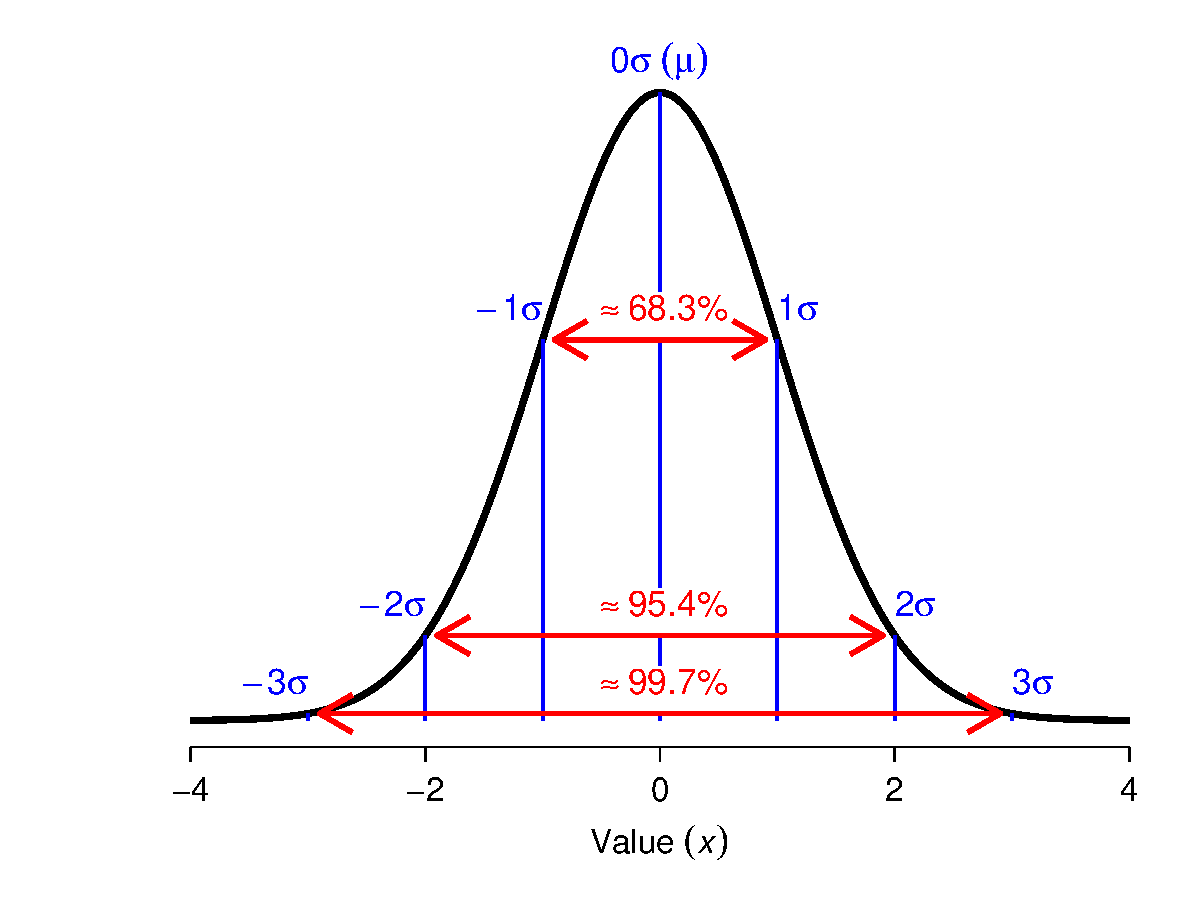
\includegraphics[keepaspectratio]{chapters/ch12_files/figure-pdf/unnamed-chunk-1-1.pdf}}
\end{center}

It must be noted that a large magnitude \emph{Z}-score does
\textbf{\emph{not}} prove that an observation is an outlier. Like
\emph{p}-values, \emph{Z}-scores are just a heuristic for making
decisions. Don't just delete any observation \(|Z|\ge\) 3; examine those
observations to see if they are legitimate and don't take any action
without a good biological reason.

\subsection{Dealing with outliers}\label{dealing-with-outliers}

\subsubsection{Deletion}\label{deletion}

The easiest way to deal with outliers is simply to delete them. This can
be fine if you have a lot of data--many 1000s or even millions of
records. I've worked with several statisticians who routinely delete
observations with response variables in the top and bottom 5
percentiles. This may not always be an appropriate strategy in biology.
For one thing, outliers can occur for completely legitimate reasons and
deleting them would be discarding important information about the study
system.

\textbf{\emph{Never}} \textbf{delete an observation based solely on its
magnitude.}

Data should only be deleted when there is a biological or experimental
reason. These might include experimental errors, inappropriate sampling,
extraordinary field conditions, etc. Furthermore, you should always
document when observations were deleted and why, and disclose that
information in your write up and to reviewers. The possibility of
including supplemental information or documents with manuscripts leaves
little excuse not to be transparent about what observations you deleted
and why.

\subsubsection{Truncation and censoring}\label{truncation-and-censoring}

\textbf{Censoring} and \textbf{truncation} are options for dealing with
extreme values. Censoring data in statistics means analyzing data as
either the measured value or the interval in which the value falls. For
example, if a mouse is weighed with a scale that goes up to 60 g, and
maxes out the scale, we record the mouse as weighing \(\ge60\) g.
Statistical methods for censored data have been developed but are
outside the scope of this course. One popular form of censoring is
called \textbf{Winsorizing}, where values below the 5th percentile are
set to the 5th percentile and values above the 95th percentile are set
to the 95th percentile. Censoring is common practice in fields involving
certain types of instrumentation. For example, many spectrophotometers
(e.g., microplate readers) record optical density (OD) as the amount of
light passing through a specimen as a measurement of concentration. Most
machines have a lower limit to the OD that they can detect. Observations
below this minimum OD might be censored to 0, or to some pre-determined
fraction of the minimum detectable OD.

Similar to censoring, outlying data can be removed by
\textbf{truncation}. Truncation in statistics means ignoring values
outside of a certain range. As with deletion, you must be very explicit
about what criteria were used to truncate the data. Just as with
deletion:

\textbf{\emph{Never}} \textbf{remove an observation based solely on its
magnitude.}

\subsubsection{Transformation}\label{transformation}

Another way to deal with outliers is to \href{@sec-trans}{transform the
data}. Variance-stabilizing transformations, such as the log-transform,
often have the side-effect of reducing the influence of outliers in the
data.

\subsubsection{Weighting}\label{weighting}

\textbf{Weighting} is a strategy where observations can be given greater
or lesser weight to adjust how much influence they have. In ordinary
least squares regression, every observation contributes equally to the
sum of squared residuals. Weighted regression instead minimizes a
weighted sum,

\[\sum_i^n{w_i\left(y_i-\hat{y_i}\right)^2}\]

where observations with smaller weights \(w_i\) have less influence on
the fitted models.

Weighting is most straightforward when the weights are known for some
external reason. For example, an observation measured with high
precision might reasonably receive more weight than an observation
measured with low precision. Choosing weights simply because
observations appear to be outliers is more difficult, because arbitrary
weights can produce arbitrary results.

One approach that formalizes this idea is \textbf{robust regression}.
Robust regression is a category of techniques that reduces the influence
of extreme observations. The most famous version is probably
\textbf{least absolute deviations} regression, which uses absolute
rather than squared deviations. Below we see a version called
\textbf{Huber M-estimator regression}, which uses iteratively-weighted
least squares to arrive at a model in which observations with small
residuals receive full weight, while observations with larger residuals
are progressively downweighted.

Here is an example of using Huber regression to fit a linear model with
less weight given to extreme values:

\begin{Shaded}
\begin{Highlighting}[]
\CommentTok{\# simulate some data}
\CommentTok{\# according to linear model}
\FunctionTok{set.seed}\NormalTok{(}\DecValTok{123}\NormalTok{)}
\NormalTok{x }\OtherTok{\textless{}{-}} \FunctionTok{sort}\NormalTok{(}\FunctionTok{runif}\NormalTok{(}\DecValTok{100}\NormalTok{, }\DecValTok{1}\NormalTok{, }\DecValTok{20}\NormalTok{))}
\NormalTok{ey }\OtherTok{\textless{}{-}} \FloatTok{1.5} \SpecialCharTok{+} \FloatTok{1.8}\SpecialCharTok{*}\NormalTok{x}
\NormalTok{y }\OtherTok{\textless{}{-}} \FunctionTok{rnorm}\NormalTok{(}\DecValTok{100}\NormalTok{, ey, }\DecValTok{2}\NormalTok{)}

\CommentTok{\# add a few extreme observations}
\NormalTok{outliers }\OtherTok{\textless{}{-}} \FunctionTok{c}\NormalTok{(}\DecValTok{95}\NormalTok{, }\DecValTok{97}\NormalTok{, }\DecValTok{99}\NormalTok{)}
\NormalTok{y[outliers] }\OtherTok{\textless{}{-}}\NormalTok{ y[outliers] }\SpecialCharTok{+} \DecValTok{20}
\NormalTok{pt.cols }\OtherTok{\textless{}{-}} \FunctionTok{rep}\NormalTok{(}\StringTok{"black"}\NormalTok{,}\DecValTok{100}\NormalTok{)}
\NormalTok{pt.cols[outliers] }\OtherTok{\textless{}{-}} \StringTok{"red"}

\CommentTok{\# make a plot}
\FunctionTok{plot}\NormalTok{(x,y, }\AttributeTok{col=}\NormalTok{pt.cols, }\AttributeTok{cex=}\FloatTok{1.4}\NormalTok{)}
\FunctionTok{legend}\NormalTok{(}\StringTok{"topleft"}\NormalTok{, }\AttributeTok{legend=}\FunctionTok{c}\NormalTok{(}\StringTok{"Possible outliers"}\NormalTok{, }\StringTok{"Not suspected outliers"}\NormalTok{),}
       \AttributeTok{col=}\FunctionTok{c}\NormalTok{(}\StringTok{"red"}\NormalTok{, }\StringTok{"black"}\NormalTok{), }\AttributeTok{cex=}\FloatTok{1.2}\NormalTok{, }\AttributeTok{pch=}\DecValTok{1}\NormalTok{)}
\end{Highlighting}
\end{Shaded}

\pandocbounded{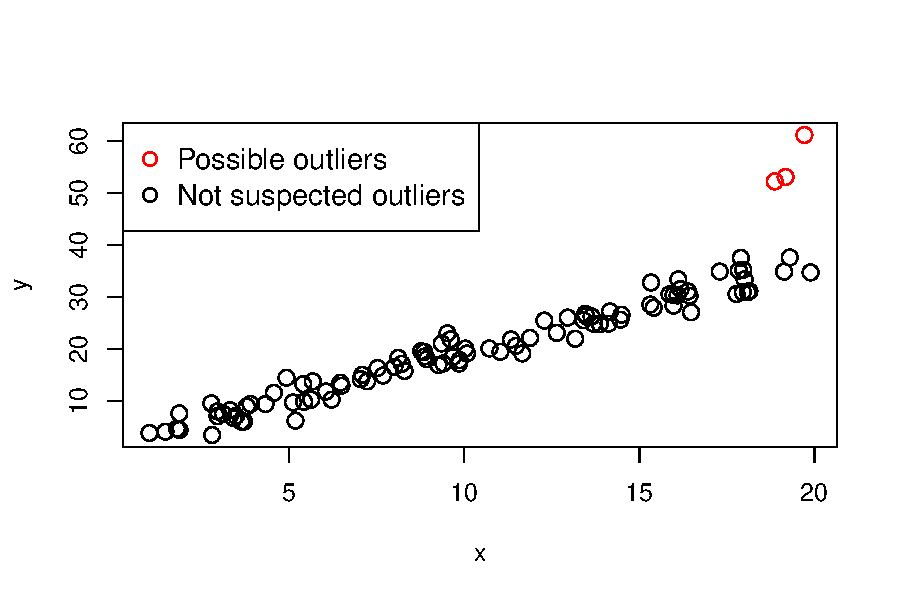
\includegraphics[keepaspectratio]{chapters/ch12_files/figure-pdf/unnamed-chunk-2-1.pdf}}

Let's compare ordinary regression with the possible outliers
(\texttt{mod1}), ordinary regression without the possible outliers
(\texttt{mod2}), and robust regression (\texttt{mod3}).

\begin{Shaded}
\begin{Highlighting}[]
\NormalTok{my.dat }\OtherTok{\textless{}{-}} \FunctionTok{data.frame}\NormalTok{(}\AttributeTok{y=}\NormalTok{y, }\AttributeTok{x=}\NormalTok{x)}
\NormalTok{mod1 }\OtherTok{\textless{}{-}} \FunctionTok{lm}\NormalTok{(y }\SpecialCharTok{\textasciitilde{}}\NormalTok{ x, }\AttributeTok{data=}\NormalTok{my.dat)}
\NormalTok{mod2 }\OtherTok{\textless{}{-}} \FunctionTok{lm}\NormalTok{(y }\SpecialCharTok{\textasciitilde{}}\NormalTok{ x, }\AttributeTok{data=}\NormalTok{my.dat[}\SpecialCharTok{{-}}\NormalTok{outliers,])}
\NormalTok{mod3 }\OtherTok{\textless{}{-}}\NormalTok{ MASS}\SpecialCharTok{::}\FunctionTok{rlm}\NormalTok{(y }\SpecialCharTok{\textasciitilde{}}\NormalTok{ x, }\AttributeTok{data=}\NormalTok{my.dat)}

\FunctionTok{plot}\NormalTok{(x, y, }\AttributeTok{col=}\NormalTok{pt.cols, }\AttributeTok{cex=}\FloatTok{1.4}\NormalTok{)}
\FunctionTok{abline}\NormalTok{(mod1, }\AttributeTok{lwd=}\DecValTok{3}\NormalTok{, }\AttributeTok{col=}\StringTok{"red"}\NormalTok{, }\AttributeTok{lty=}\DecValTok{2}\NormalTok{)}
\FunctionTok{abline}\NormalTok{(mod2, }\AttributeTok{lwd=}\DecValTok{3}\NormalTok{)}
\FunctionTok{abline}\NormalTok{(mod3, }\AttributeTok{lwd=}\DecValTok{3}\NormalTok{, }\AttributeTok{col=}\StringTok{"blue"}\NormalTok{, }\AttributeTok{lty=}\DecValTok{3}\NormalTok{)}
\FunctionTok{legend}\NormalTok{(}\StringTok{"topleft"}\NormalTok{,}
       \AttributeTok{legend=}\FunctionTok{c}\NormalTok{(}\StringTok{"OLS with outliers"}\NormalTok{,}
                \StringTok{"OLS without outliers"}\NormalTok{,}
                \StringTok{"Robust regression"}\NormalTok{),}
       \AttributeTok{lwd=}\DecValTok{3}\NormalTok{, }\AttributeTok{lty=}\FunctionTok{c}\NormalTok{(}\DecValTok{2}\NormalTok{,}\DecValTok{1}\NormalTok{,}\DecValTok{3}\NormalTok{),}
       \AttributeTok{col=}\FunctionTok{c}\NormalTok{(}\StringTok{"red"}\NormalTok{,}\StringTok{"black"}\NormalTok{,}\StringTok{"blue"}\NormalTok{),}
       \AttributeTok{cex=}\FloatTok{1.2}\NormalTok{)}
\end{Highlighting}
\end{Shaded}

\pandocbounded{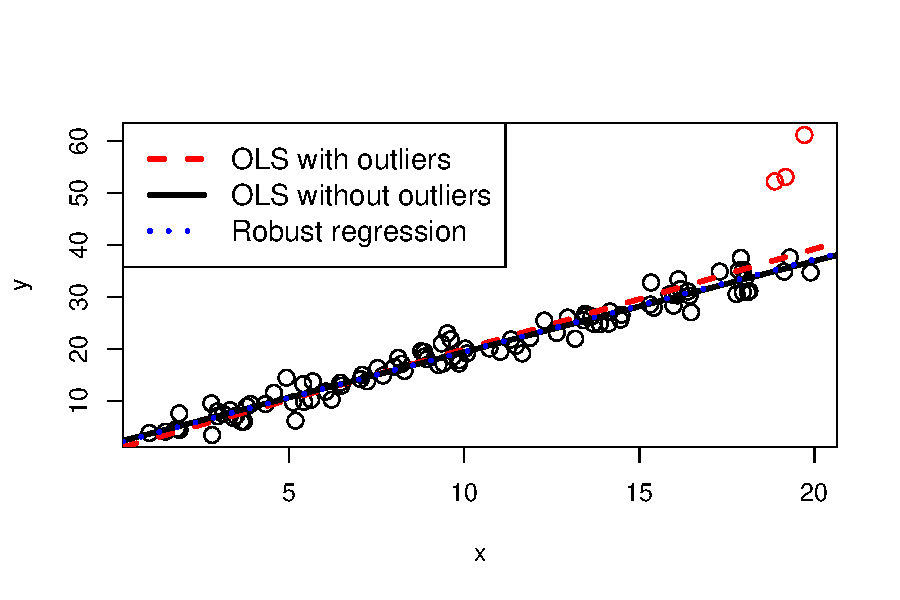
\includegraphics[keepaspectratio]{chapters/ch12_files/figure-pdf/unnamed-chunk-3-1.pdf}}

The robust regression finds a line very similar to the model without the
outliers, but does so without discarding data.

\subsubsection{Alternative strategies}\label{alternative-strategies}

Finally, researchers can use analysis strategies that are less sensitive
to outliers. As mentioned above, there are is a large class of
\textbf{robust statistics} that use different strategies to give
suspected outliers much less influence than under conventional methods
based on sums of squared errors. \textbf{Nonparametric methods},
particularly those based on rank order, can also be less sensitive to
outliers.

Whatever strategy you choose to deal with your outliers, you need to be
aware of how much your decision affected the outcome. It is a good idea
to analyze your data both with and without suspected outliers to measure
how much influence they really have. If the analysis returns the same
results with and without the outliers, leave them in.

\section{Autocorrelation}\label{sec-problems-auto}

Autocorrelation describes a phenomenon where set of values is correlated
with itself, with the strength of that correlation determined by the
distance between observations. In biology, the ``distance'' that defines
autocorrelation is often spatial, temporal, or phylogenetic.

{\def\LTcaptype{none} % do not increment counter
\begin{longtable}[]{@{}
  >{\raggedright\arraybackslash}p{(\linewidth - 4\tabcolsep) * \real{0.1528}}
  >{\raggedright\arraybackslash}p{(\linewidth - 4\tabcolsep) * \real{0.1528}}
  >{\raggedright\arraybackslash}p{(\linewidth - 4\tabcolsep) * \real{0.6944}}@{}}
\toprule\noalign{}
\begin{minipage}[b]{\linewidth}\raggedright
Autocorrelation type
\end{minipage} & \begin{minipage}[b]{\linewidth}\raggedright
Distance measure
\end{minipage} & \begin{minipage}[b]{\linewidth}\raggedright
Explanation
\end{minipage} \\
\midrule\noalign{}
\endhead
\bottomrule\noalign{}
\endlastfoot
Spatial & Space (e.g., km) & Samples from sites that are close together
in space are more similar to each other than they are to sites that are
farther away, just because they are closer to each other. \\
Temporal & Time (e.g., days) & Observations taken closer together in
time are more similar to each other than they are to observations
separated by more time. \\
Phylogenetic & Relatedness & Taxa that share a more recent common
ancestor (i.e., are more closely related) are more similar to each other
than they are to taxa that are less closely related to each other. \\
\end{longtable}
}

The main consequence of autocorrelation is similar to the problems
associated with pseudoreplication: because observations are not
independent, the statistically relevant number of observations (degrees
of freedom) is smaller than the nominal number of observations. This
means that the power of the test is inflated. A related idea is that the
residuals of a statistical model can be autocorrelated. In that case,
the model violates the assumption of independent residuals shared by
most statistical methods. Autocorrelation can be controlled for if you
have some idea of its source and nature.

\subsection{Graphical methods to identify
autocorrelation}\label{sec-problems-auto-graph}

One way to explore potential autocorrelation is to construct a
variogram. A variogram plots the squared differences between samples
against their distance (temporal, spatial, etc.). A semivariogram uses
half of that variance. An example semivariogram is below.

This figure shows some important quantities on the semivariogram:

\pandocbounded{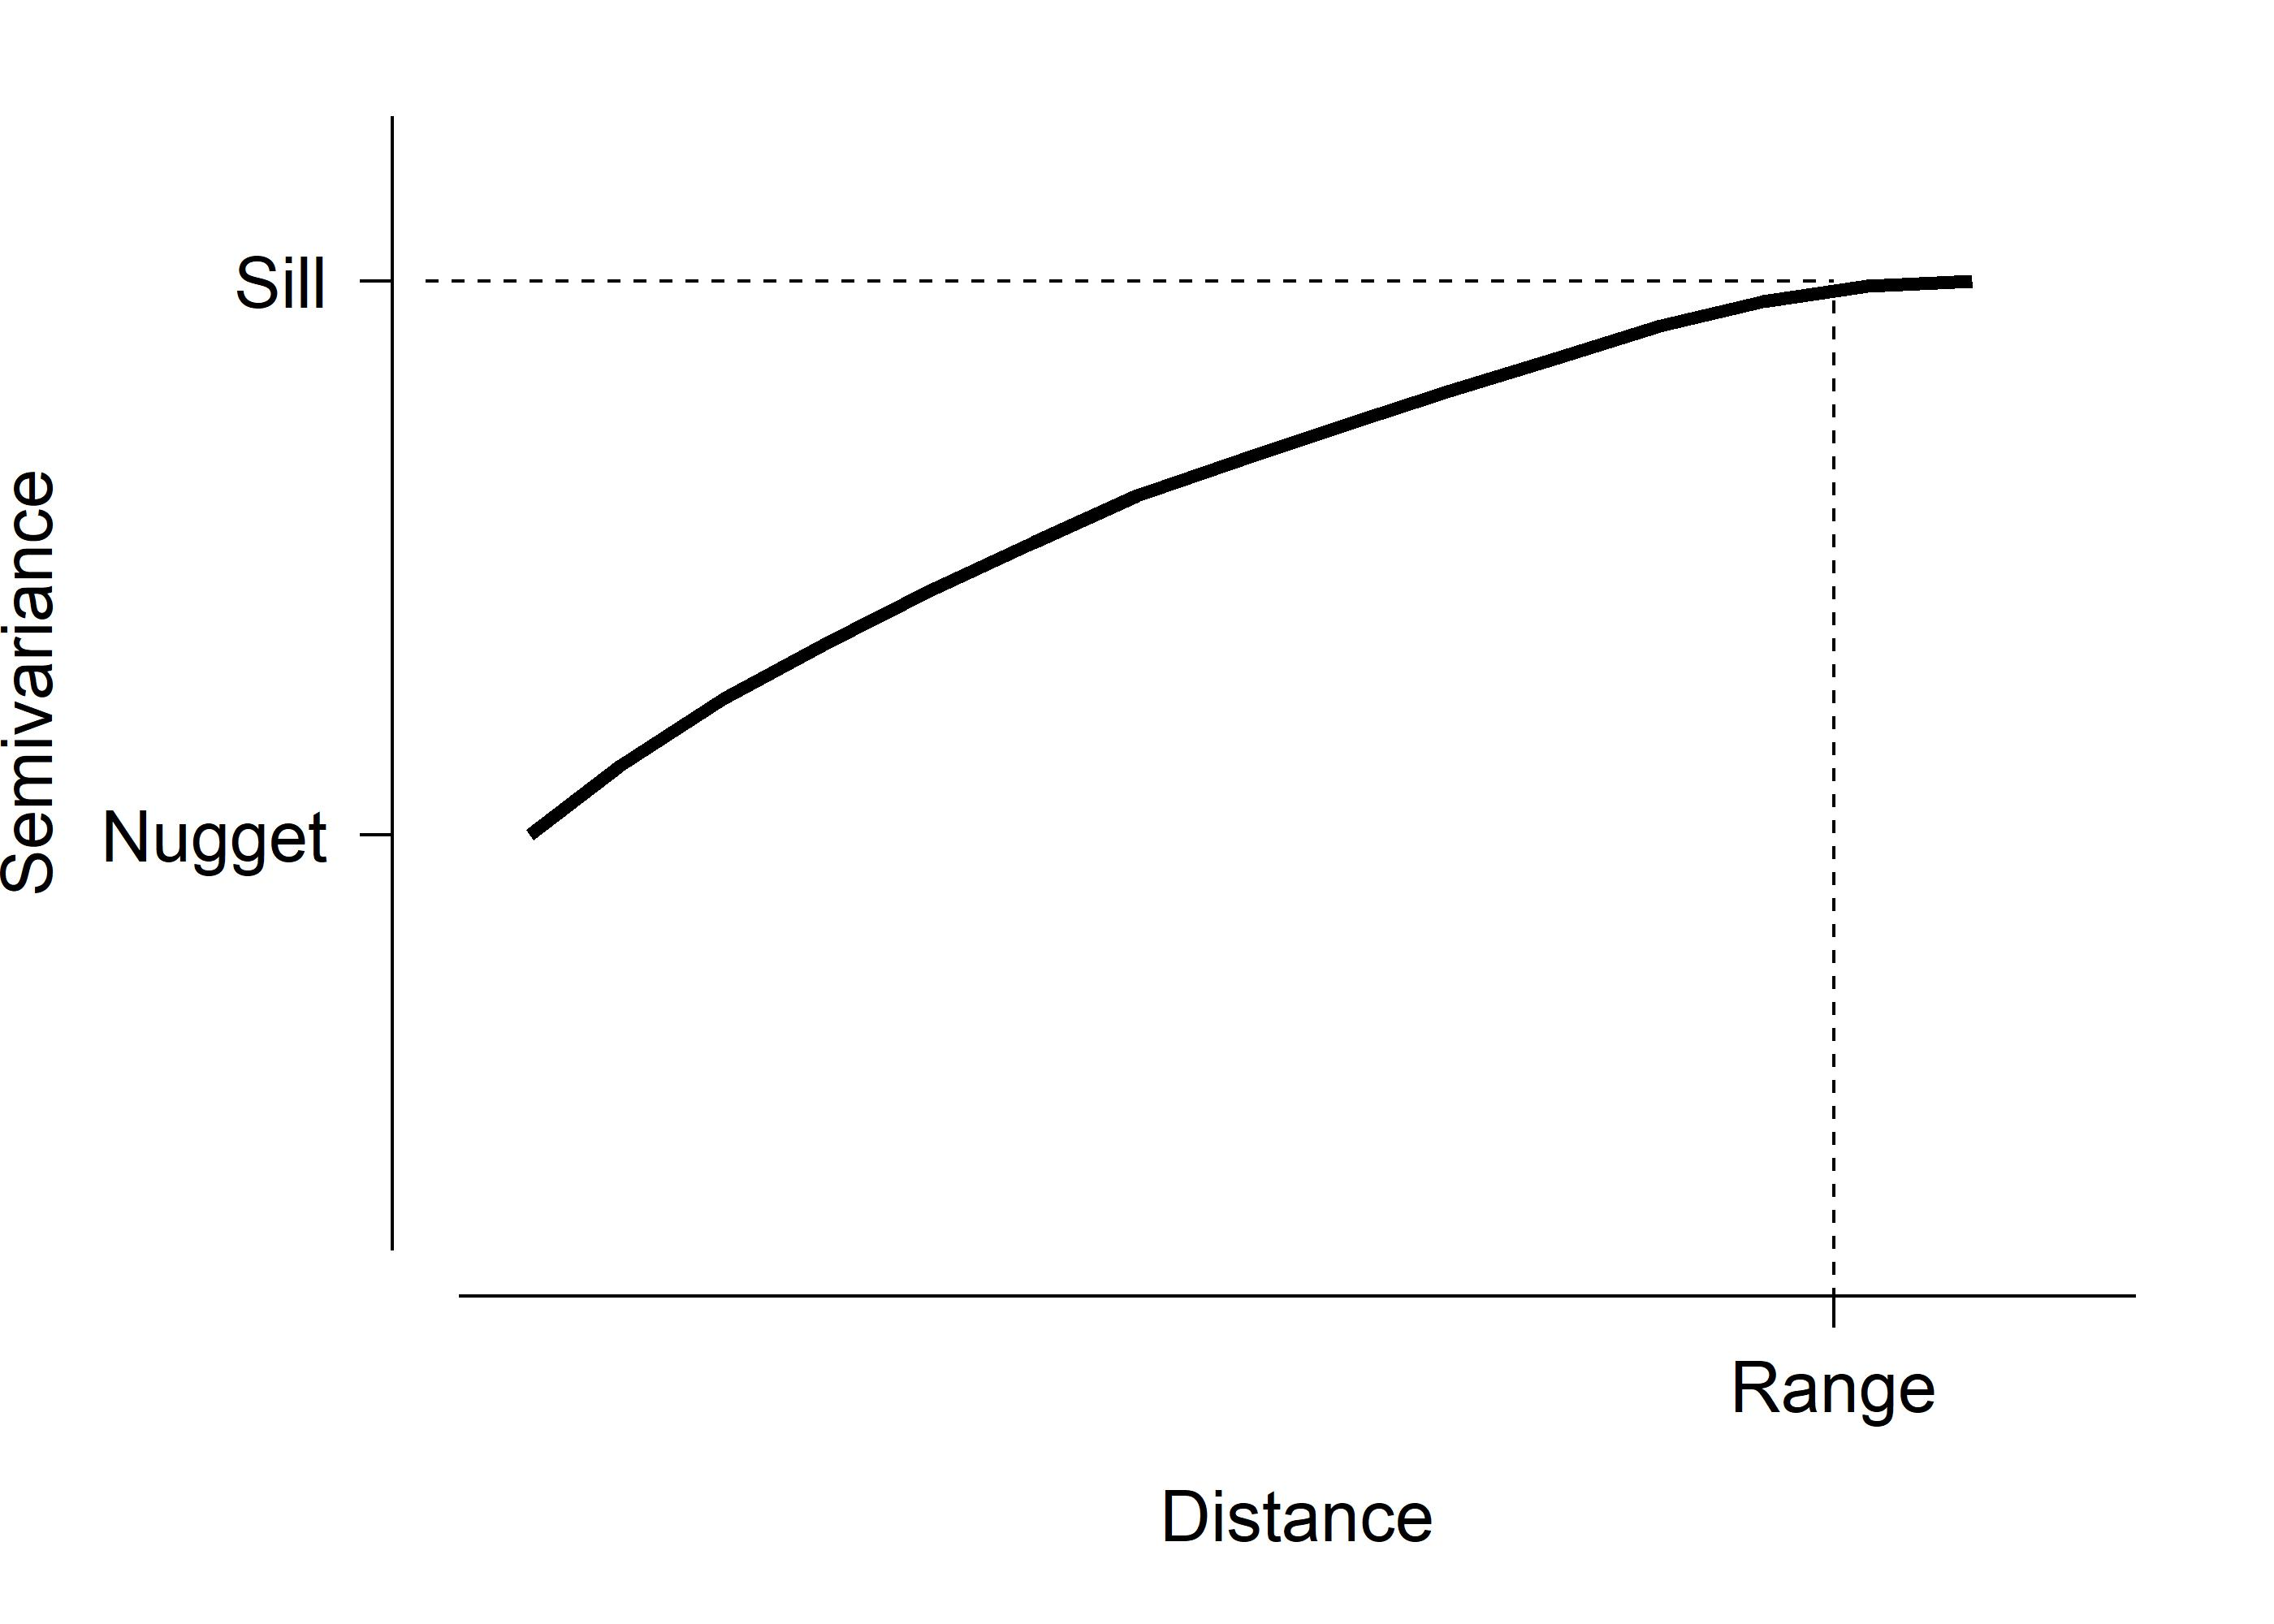
\includegraphics[keepaspectratio,alt={Anatomy of a semivariogram. Semivariance increases with the distance between observations until reaching the sill. The range is the distance at which the sill is reached, beyond which observations are no longer spatially autocorrelated. The nugget represents variation at very short distances, including fine-scale variation and measurement error.}]{chapters/../images/12-01.jpg}}\{alt-text:
``Schematic semivariogram with distance on the x-axis and semivariance
on the y-axis. A curved line begins above zero at the labeled nugget,
increases with distance, and levels off at the labeled sill. A vertical
dashed line marks the range, where the curve reaches the sill.''\}

\begin{itemize}
\tightlist
\item
  \textbf{Nugget}: The variance or semivariance at 0 or very short
  distance. This represents other sources of error, such as sampling
  error, demographic stochasticity, etc.
\item
  \textbf{Sill}: The variance or semivariance at which the curve gets
  close to its maximum or asymptotic value.
\item
  \textbf{Range}: The distance at which the variance or semivariance
  reaches the sill. Samples at distances beyond the range are considered
  no longer spatially autocorrelated.
\end{itemize}

Semivariograms should always increase, at least initially, because
closer observations should be similar to each other simply as a matter
of proximity. Samples separated by distances less than the range are
autocorrelated. Semivariograms sometimes reach a peak and then start
decreasing, or varying up and down. The initial peak is usually
interpreted as the sill, and the distance when the curve reaches the
sill is considered the range. The importance and interpreation of the
semivariogram is something that you, as a biologist, have to figure out.

\subsection{Mantel tests for
autocorrelation}\label{sec-problems-auto-mantel}

\textbf{Spatial autocorrelation} is an ever-present problem for
ecologists and environmental biologists: observations that are closer
together in space might be similar to each other in terms of biology,
just because they are closer together. The cause of that spatial
autocorrelation determines how you need to deal with it in your
analysis.

The fact that observations close together in space tend to be more
similar is not in and of itself a problem. There can be a strong spatial
structure in the data that is explained by predictors like latitude,
longitude, or some environmental gradient. In other words, the spatial
structure may be what you are trying to discover in the first place.

Where spatial structure becomes a problem is in the \emph{residuals} of
your analysis. If the residuals contain spatial structure \emph{after
accounting for environmental and other predictors}, then there is a
problem called ``lack of independence''. This means that observations
contain less independent information than the model assumes.
Consequently the analysis is conducted with more degrees of freedom than
there really are. This inflates the power of the test, increasing the
possibility of a false positive (a Type I error).

Historically, biologists often used a
\href{@sec-mtest-mantel}{\textbf{Mantel test}} to test for spatial
autocorrelation in the response variable. Briefly, the Mantel test can
be thought of as a multivariate generalization of linear correlation
that measures correlation between two matrices. Whereas linear
correlation measures how variation in one variable is related to
variation in another variable, the Mantel test measures how variation in
one matrix is related to variation in another matrix. But given what you
just read, you should now recognize that as insufficient:

\begin{enumerate}
\def\labelenumi{\arabic{enumi}.}
\tightlist
\item
  autocorrelation in response \emph{values} is not necessarily a problem
  if it can be modeled by predictor variables;
\item
  autocorrelation in model residuals is where the problem lies; and,
\item
  a Mantel test can fail to detect distance decay in response values,
  even when residuals are spatially dependent.
\end{enumerate}

Nowadays, we have a tests specifically designed for measuring spatial
autocorrelations. One of the most common is \textbf{Moran's}
\textbf{\emph{I}}. This is a common measure of spatial autocorrelation
that is easy to interpret: \(I>0\) means that nearby observations are
more similar than expected; \(I\approx0\) means little evidence of
spatial autocorrelation; and \(I<0\) means that nearby observations tend
to be more dissimilar to each other than expected.

The ``than expected'' part refers to the amount of similarity expected
if the values were distributed randomly with respect to the specified
spatial relationships among observations..

We will illustrate use of Moran's \emph{I} in a future module. For now,
the basic procedure is to:

\begin{enumerate}
\def\labelenumi{\arabic{enumi}.}
\tightlist
\item
  Define spatial weights for each pair of observations (a kind of
  distance matrix). These could be based on a distance threshold,
  nearest neighbors, or geographic distance.
\item
  Fit your model (regression, GLM, or whatever).
\item
  Test for spatial autocorrelation of the model residuals by calculating
  Moran's \emph{I} using the spatial weights. One option is the function
  \texttt{spdep::moran.test()}.
\end{enumerate}

\subsection{Dealing with autocorrelation}\label{sec-problems-auto-deal}

If you detect significant autocorrelation, don't panic. Autocorrelation
may or may not be a problem in your dataset. As pointed out by Kuehn and
Dormann (2012), there is a difference between autocorrelation in a
response variable and autocorrelation in the residuals of a statistical
model. Autocorrelation in a response variable can be managed by
inclusion of appropriate predictor variables. This works because if
autocorrelated values can be predicted by a predictor variable, then it
won't be present in the residuals.

Autocorrelation in residuals, however, represents spatial structure that
is not accounted for by the model. There are methods for accounting for
autocorrelated residuals such as generalized least squares models (GLS)
with spatial correlation structures (Zuur \emph{et al.} 2007),
conditional autoregressive models (CAR) (Gelfand and Vounatsou 2003),
and mixed models that explicitly account for spatial dependence (Bolker
\emph{et al.} 2009). Other approaches may incorporate spatial predictors
or smooth spatial trends directly into the model. None of these
solutions is appropriate for every situation, so consider the likely
cause and spatial scale of the autocorrelation, the goals of the
analysis, and what your data can support.

\section{Collinearity}\label{sec-problems-collin}

Sometimes we face the problem of having predictor variables that are not
only related to the response variable, but also related to each other.
This phenomenon is called \textbf{collinearity}. In large datasets the
problem becomes \textbf{multicollinearity}, when many variables are
related to each other. Including collinear predictor variables in an
analysis can severely bias the parameter estimates of that analysis
(e.g., regression coefficients) and as a result make the results
misleading or not generalizable. The effects of collinear predictor
variables are by definition confounded with each other, meaning that the
effects cannot be separated (Dormann \emph{et al.} 2013).

The most straightforward way of detecting collinearity is with
scatterplot matrices and correlation coefficients (see
Section~\ref{sec-plot1-many-pair}). This is a technique to visualize how
many variables in a dataset relate to each other simultaneously. As
shown in the linked section, replacing the upper triangle of boxes with
the correlation coefficients can help detect potentially problematic
pairs of variables. The figure below shows an example from the
\texttt{crabs} dataset in package \texttt{MASS}. In this dataset, all of
the variables are highly correlated with each other. Using more than one
of them as a predictor in a model would make it hard for the algorithm
to distinguish their effects from each other.

\begin{center}
\pandocbounded{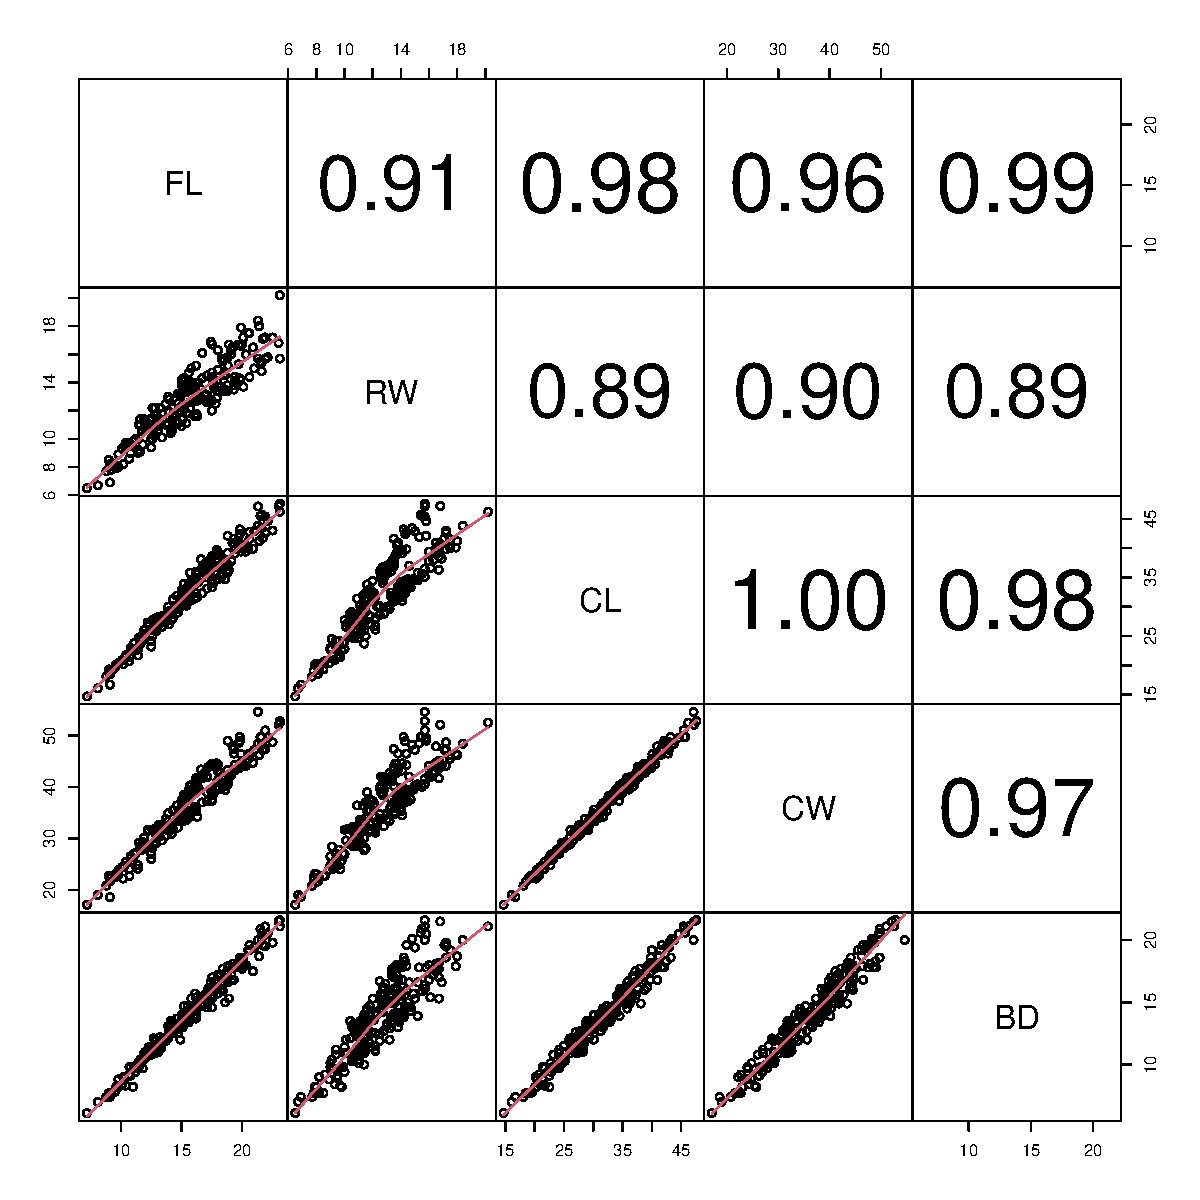
\includegraphics[keepaspectratio]{chapters/ch12_files/figure-pdf/unnamed-chunk-4-1.pdf}}
\end{center}

If you have many variables, then a figure like the one above can be hard
to read or interpret. One solution might be to create a table of
correlation coefficients between every pair of variables. The base
function \texttt{cor()} can do this, but a better-formatted table takes
a little more work.

\begin{Shaded}
\begin{Highlighting}[]
\FunctionTok{data}\NormalTok{(crabs, }\AttributeTok{package=}\StringTok{"MASS"}\NormalTok{)}
\NormalTok{x }\OtherTok{\textless{}{-}}\NormalTok{ crabs}
\NormalTok{dat.cols }\OtherTok{\textless{}{-}} \DecValTok{4}\SpecialCharTok{:}\DecValTok{8}
\FunctionTok{cor}\NormalTok{(x[,dat.cols])}
\end{Highlighting}
\end{Shaded}

\begin{verbatim}
          FL        RW        CL        CW        BD
FL 1.0000000 0.9069876 0.9788418 0.9649558 0.9876272
RW 0.9069876 1.0000000 0.8927430 0.9004021 0.8892054
CL 0.9788418 0.8927430 1.0000000 0.9950225 0.9832038
CW 0.9649558 0.9004021 0.9950225 1.0000000 0.9678117
BD 0.9876272 0.8892054 0.9832038 0.9678117 1.0000000
\end{verbatim}

\begin{Shaded}
\begin{Highlighting}[]
\CommentTok{\# same table as a data frame:}
\NormalTok{vars }\OtherTok{\textless{}{-}} \FunctionTok{names}\NormalTok{(x)[dat.cols]}

\CommentTok{\# generate every unique pair of two variables by name:}
\NormalTok{cx }\OtherTok{\textless{}{-}} \FunctionTok{data.frame}\NormalTok{(}\FunctionTok{t}\NormalTok{(}\FunctionTok{combn}\NormalTok{(vars, }\DecValTok{2}\NormalTok{)))}

\CommentTok{\# calculate correlation coefficients for each pair:}
\NormalTok{cx}\SpecialCharTok{$}\NormalTok{r }\OtherTok{\textless{}{-}} \ConstantTok{NA}
\ControlFlowTok{for}\NormalTok{(i }\ControlFlowTok{in} \DecValTok{1}\SpecialCharTok{:}\FunctionTok{nrow}\NormalTok{(cx))\{}
\NormalTok{    cx}\SpecialCharTok{$}\NormalTok{r[i] }\OtherTok{\textless{}{-}} \FunctionTok{cor}\NormalTok{(x[,cx}\SpecialCharTok{$}\NormalTok{X1[i]], x[,cx}\SpecialCharTok{$}\NormalTok{X2[i]])}
\NormalTok{\}}
\NormalTok{cx}
\end{Highlighting}
\end{Shaded}

\begin{verbatim}
   X1 X2         r
1  FL RW 0.9069876
2  FL CL 0.9788418
3  FL CW 0.9649558
4  FL BD 0.9876272
5  RW CL 0.8927430
6  RW CW 0.9004021
7  RW BD 0.8892054
8  CL CW 0.9950225
9  CL BD 0.9832038
10 CW BD 0.9678117
\end{verbatim}

The resulting table can then be sorted or filtered by \texttt{r} to
identify pairs of variables that are correlated with each other.

\begin{Shaded}
\begin{Highlighting}[]
\CommentTok{\# not run:}
\CommentTok{\# filter to |r| \textgreater{} 0.7}
\NormalTok{cx[}\FunctionTok{which}\NormalTok{(}\FunctionTok{abs}\NormalTok{(cx}\SpecialCharTok{$}\NormalTok{r) }\SpecialCharTok{\textgreater{}} \FloatTok{0.7}\NormalTok{),]}
\end{Highlighting}
\end{Shaded}

Dormann \emph{et al.} (2013) suggest to use a cutoff of \(|r|\) in
between 0.5 and 0.7 to identify collinear pairs of variables. When a
pair of variables are identified as collinear, the easiest solution is
to simply run the analysis without one of them. This is because the
variables are redundant, and any conclusions made using one would also
be obtained using the other.

\section{Missing data}\label{sec-problems-miss}

The last target of exploratory data analysis that we will explore is
\textbf{missing data}. Data can be missing for many reasons. Equipment
failures, human error, natural disasters, and other causes can cause
values in your dataset to go missing or otherwise be invalid. How to
handle the missing data is up to you as a biologist: \emph{there is no
one-size-fits-all statistical solution}. The two basic ways to deal with
missing data are to (1) not deal with it and (2) estimate the missing
values.

\subsection{Option 1: Ignore missing
data}\label{sec-problems-miss-ignore}

The easiest solution is simply to ignore missing data. Consider
\href{../datasets/missing-data-example.csv}{this dataset}, which
contains morphological data on 63 species of bats (Hutcheon \emph{et
al.} 2002). Notice that in this version the brain masses (\texttt{brw})
are missing for 3 species of bats.

\begin{Shaded}
\begin{Highlighting}[]
\CommentTok{\# replace with your working directory and path!}
\NormalTok{in.name }\OtherTok{\textless{}{-}} \StringTok{"../datasets/missing{-}data{-}example.csv"}
\NormalTok{dat }\OtherTok{\textless{}{-}} \FunctionTok{read.csv}\NormalTok{(in.name, }\AttributeTok{header=}\ConstantTok{TRUE}\NormalTok{)}
\end{Highlighting}
\end{Shaded}

Because there are a lot of data, one option for analyzing this dataset
would be to simply ignore the missing observations. For example, if
someone was interested in the relationship between body size (variable
\texttt{bow}) and brain mass, they could just fit a model and R would
(for most methods) automatically ignore missing values. Note that in
this example both variables are log-transformed to ensure normality and
positivity.

\begin{Shaded}
\begin{Highlighting}[]
\NormalTok{dat}\SpecialCharTok{$}\NormalTok{logbw }\OtherTok{\textless{}{-}} \FunctionTok{log}\NormalTok{(dat}\SpecialCharTok{$}\NormalTok{bow)}
\NormalTok{dat}\SpecialCharTok{$}\NormalTok{logbr }\OtherTok{\textless{}{-}} \FunctionTok{log}\NormalTok{(dat}\SpecialCharTok{$}\NormalTok{brw)}

\NormalTok{mod1 }\OtherTok{\textless{}{-}} \FunctionTok{lm}\NormalTok{(logbr}\SpecialCharTok{\textasciitilde{}}\NormalTok{logbw, }\AttributeTok{data=}\NormalTok{dat)}
\FunctionTok{summary}\NormalTok{(mod1)}
\end{Highlighting}
\end{Shaded}

\begin{verbatim}

Call:
lm(formula = logbr ~ logbw, data = dat)

Residuals:
     Min       1Q   Median       3Q      Max 
-0.82879 -0.16408  0.05009  0.19548  0.35881 

Coefficients:
            Estimate Std. Error t value Pr(>|t|)    
(Intercept)  3.96599    0.09476   41.85   <2e-16 ***
logbw        0.75322    0.02881   26.14   <2e-16 ***
---
Signif. codes:  0 '***' 0.001 '**' 0.01 '*' 0.05 '.' 0.1 ' ' 1

Residual standard error: 0.2616 on 58 degrees of freedom
  (3 observations deleted due to missingness)
Multiple R-squared:  0.9218,    Adjusted R-squared:  0.9204 
F-statistic: 683.4 on 1 and 58 DF,  p-value: < 2.2e-16
\end{verbatim}

The parameter estimates of intercept = \texttt{3.9659} and slope =
\texttt{0.7532} are very close to the values obtained using the full
dataset of \texttt{3.9685} and \texttt{0.7516}. In this case, ignoring
the missing data worked just fine.

\subsection{Option 2: Interpolate or impute missing
data}\label{sec-problems-miss-inter}

If you need to replace the missing data, then the best option is to
\textbf{interpolate} or \textbf{impute} them. How exactly to do this
depends on the question being asked. If there is a clear relationship
between the variable with missing values and another variable, then you
can use that relationship to estimate the missing values. You can also
use \textbf{multiple imputation} to estimate the missing values using
information from several related variables at once. The example below
illustrates simple interpolation (aka: single imputation) to replace the
missing brain weights using known body masses.

\begin{Shaded}
\begin{Highlighting}[]
\CommentTok{\# flag missing observations}
\NormalTok{flag }\OtherTok{\textless{}{-}} \FunctionTok{which}\NormalTok{(}\FunctionTok{is.na}\NormalTok{(dat}\SpecialCharTok{$}\NormalTok{brw))}

\CommentTok{\# log transform (if not done already)}
\NormalTok{dat}\SpecialCharTok{$}\NormalTok{logbw }\OtherTok{\textless{}{-}} \FunctionTok{log}\NormalTok{(dat}\SpecialCharTok{$}\NormalTok{bow)}
\NormalTok{dat}\SpecialCharTok{$}\NormalTok{logbr }\OtherTok{\textless{}{-}} \FunctionTok{log}\NormalTok{(dat}\SpecialCharTok{$}\NormalTok{brw)}

\CommentTok{\# fit model}
\NormalTok{mod1 }\OtherTok{\textless{}{-}} \FunctionTok{lm}\NormalTok{(logbr}\SpecialCharTok{\textasciitilde{}}\NormalTok{logbw, }\AttributeTok{data=}\NormalTok{dat)}

\CommentTok{\# predict missing logbr at logbw}
\NormalTok{px }\OtherTok{\textless{}{-}} \FunctionTok{data.frame}\NormalTok{(}\AttributeTok{logbw=}\NormalTok{dat}\SpecialCharTok{$}\NormalTok{logbw[flag])}
\NormalTok{pr }\OtherTok{\textless{}{-}} \FunctionTok{predict}\NormalTok{(mod1, }\AttributeTok{newdata=}\FunctionTok{data.frame}\NormalTok{(px))}

\CommentTok{\# insert predicted values}
\NormalTok{dat}\SpecialCharTok{$}\NormalTok{logbr[flag] }\OtherTok{\textless{}{-}}\NormalTok{ pr}

\CommentTok{\# back{-}transform to original scale}
\NormalTok{dat}\SpecialCharTok{$}\NormalTok{brw[flag] }\OtherTok{\textless{}{-}} \FunctionTok{exp}\NormalTok{(dat}\SpecialCharTok{$}\NormalTok{logbr[flag])}
\end{Highlighting}
\end{Shaded}

The interpolated values are similar to the true values, but with quite a
bit of error. The term of art here is ``correct to an order of
magnitude''.

\begin{Shaded}
\begin{Highlighting}[]
\NormalTok{dat}\SpecialCharTok{$}\NormalTok{brw[flag]}
\end{Highlighting}
\end{Shaded}

\begin{verbatim}
[1]  729.7784  507.7160 2138.6809
\end{verbatim}

\begin{Shaded}
\begin{Highlighting}[]
\NormalTok{true.vals }\OtherTok{\textless{}{-}} \FunctionTok{c}\NormalTok{(}\DecValTok{597}\NormalTok{, }\DecValTok{543}\NormalTok{, }\DecValTok{2070}\NormalTok{)}

\CommentTok{\# percentage bias in interpolated values:}
\DecValTok{100} \SpecialCharTok{*}\NormalTok{ (dat}\SpecialCharTok{$}\NormalTok{brw[flag]}\SpecialCharTok{{-}}\NormalTok{true.vals) }\SpecialCharTok{/}\NormalTok{ true.vals}
\end{Highlighting}
\end{Shaded}

\begin{verbatim}
[1] 22.240932 -6.497972  3.317919
\end{verbatim}

Interpolation can be improved by predicting the missing values using
additional variables. Multiple imputation, like any statistical model,
can suffer from the effects of multicollinearity in the ``predictors'',
so be mindful that you don't obtain--and use--biased estimates of your
missing values. Penone \emph{et al.} (2014) reviewed some strategies for
imputing missing data in the context of life history traits, but the
approaches could be applied to other areas of biology.

\chapter{Planning your data analysis}\label{sec-plan}

One of the main questions that biologists have after collecting data is,
``What statistical test do I use?'' Ignoring the fact that they should
have thought about that \textbf{\emph{before collecting their data}},
the answer to that question depends on the answers to two other
questions:

\begin{enumerate}
\def\labelenumi{\arabic{enumi}.}
\tightlist
\item
  What question are you trying to answer?
\item
  What kind of data do you have?
\end{enumerate}

After \href{@sec-desc}{exploring the data}, \href{@sec-summ}{summarizing
the data}, \href{@sec-dist}{thinking about distributions},
\href{@sec-dtest}{checking data distributions}, and gaining an
understanding of the \href{@sec-plot1}{patterns} and
\href{@sec-problem}{problems} in a dataset, it is time to run the main
analysis. This guide is designed to help you use what you learned in
exploring the data to choose an appropriate analytical strategy.

\section{How to use this guide}\label{sec-plan-how}

The sections below list some common analysis strategies that you might
use for some common types of biological questions, and guides you
through the selection process. This document is meant to serve as a
primer and rough guide; it is not meant to be exhaustive. This document
is also very much a work in progress. Not every situation is covered,
and there might be issues in your dataset that make the recommendations
below problematic.

Each section is structured as a dichotomous key, because biologists love
dichotomous keys. At each step, choose the option that best applies to
your situation If you don't know the answer to a question or which
option to choose, you may need to go back and do some more exploratory
data analysis. R functions are provided for most methods.

\section{What question are you trying to
answer?}\label{sec-plan-question}

\subsection{Quantifying your question}\label{sec-plan-question-quant}

The first thing to nail down is what \emph{statistical question} you are
trying to answer. This does not mean what \emph{biological question} you
are investigating, but two are related. An example biological question
might be:

\textbf{How do small mammals (rodents) adapt to live in urban
environments?}

This is a good biological question, but it is \emph{not} a question that
you can answer with statistics. In order to answer the overarching
biological question, we usually need to break it down into smaller
chunks: hypotheses that can either be true or false, and predictions
(patterns in the data) that would be observed if the hypothesis is true
and not observed if a hypothesis is false. For the question above, we
might have some working hypothesis like:

\textbf{Rodents living in urban environments shift their diet to take
advantage of anthropogenic food sources.}

This is a good scientific hypothesis, because it is
\textbf{falsifiable}. For this or any other hypothesis we need to be
able to define:

\begin{enumerate}
\def\labelenumi{\arabic{enumi}.}
\tightlist
\item
  What would we observe if the hypothesis is not true?
\item
  What would we observe if the hypothesis is true?
\end{enumerate}

For this statement, these are relatively straightforward. We are are
closer to a statistical hypothesis, but we're not quite there yet. What
does it mean to ``shift their diet''? Compared to what? How do we
quantify a ``shift''?

To make a statistical hypothesis we need to think of \emph{specific
quantitative or categorical comparisons that would support or contradict
the hypothesis}. For example, here are a few of the potential
predictions implied by the hypothesis above:

\begin{itemize}
\tightlist
\item
  Rodents in urban environments will have a \textbf{greater proportion}
  of artificial foods in their feces than conspecific rodents in rural
  or natural environments.
\item
  Rodents in urban environments will consume a \textbf{smaller number}
  of different kinds of food than rodents in rural environments because
  of the availability of calorie-dense foods associated with humans.
\item
  Rodents in urban environments will spend \textbf{less} time foraging
  and make \textbf{shorter} foraging movements than rodents in rural or
  natural environments.
\item
  Stable isotope ratios of whole-body tissues in urban animals will be
  \textbf{different than} those ratios in rural animals.
\item
  Serum triglyceride concentrations will be \textbf{correlated with}
  amount of impervious surface within 150 m of their home range.
\end{itemize}

These predictions are statements of the kinds of patterns that we should
observe if the hypothesis was true. Note the bolded parts: these are
quantitative comparisons that can be true or not true.

We can also define their logical negation: what would we observe if the
hypothesis was not true? Critically, these predictions include
comparison phrases like \textbf{greater than} or \textbf{smaller number
of} or \textbf{less time than}. Those comparisons are the sorts of
patterns that a statistical model can actually evaluate. Knowing what
kind of pattern you are testing is a key step in planning your data
analysis.

\subsection{Types of questions}\label{sec-plan-question-types}

Broadly speaking, statistical hypotheses in biology tend to fall into
just a few categories:

\begin{enumerate}
\def\labelenumi{\arabic{enumi}.}
\tightlist
\item
  Testing for a \emph{difference in mean or location} between groups.
\item
  Testing for a \emph{continuous relationship} between a response
  variable (or multiple variables) and one or more predictor variables.
  Also referred to as ``predicting'' or ``modeling'' a continuous
  variable.
\item
  Testing for (lack of) \emph{independence between categories} of
  observations.
\item
  \emph{Classifying} observations based on predictor variables.
\end{enumerate}

These categories are not mutually exclusive. Many questions phrased as
one category can be reframed into another. How you frame your question
depends on many factors and at some point will involve some discretion
on your part. \emph{There is often more than one right way analyze a
dataset}, but the right ways are a vanishingly small subset of the
possible ways to analyze your data.

\section{Testing for a difference in mean or
location}\label{sec-plan-meanloc}

\textbf{Dichotomous key for testing for a difference in mean or
location:}

\begin{description}
\tightlist
\item[\textbf{1.}]
Single response variable (or one variable tested at a time) → \textbf{3}
\item[\textbf{1′.}]
Multiple response variables tested at once → \textbf{2}
\item[\textbf{2.}]
Data are appropriate for a parametric multivariate analysis → Try
\href{@sec-mtest-group-man}{MANOVA}.\\
R function: \texttt{manova()}.
\item[\textbf{2′.}]
Data are not appropriate for MANOVA, or differences are being measured
using a distance or dissimilarity measure → Try
\href{@sec-mtest-group-perm}{permutational MANOVA (PERMANOVA)}.\\
R function: \texttt{vegan::adonis2()}.
\item[\textbf{3.}]
Need to compare values in one group to a target value → \textbf{4}
\item[\textbf{3′.}]
Need to compare values in one group to values in at least one other
group → \textbf{5}
\item[\textbf{4.}]
Data are appropriate for a parametric test → Try a one-sample
\emph{t}-test.\\
R function: \texttt{t.test()}.
\item[\textbf{4′.}]
Data are not appropriate for a parametric test → Try a one-sample
Wilcoxon signed-rank test.\\
R function: \texttt{wilcox.test()}.
\item[\textbf{5.}]
Comparing two groups in a simple design → \textbf{6}
\item[\textbf{5′.}]
Comparing more than two groups, or using a more complex design involving
multiple factors, interactions, blocking, or repeated measures →
\textbf{7}
\item[\textbf{6.}]
Data are appropriate for a parametric test → Try a
\href{@sec-groups-2samp-2t}{two-sample \emph{t}-test}, including a
paired \emph{t}-test if observations are paired or matched.\\
R function: \texttt{t.test()}.
\item[\textbf{6′.}]
Data are not appropriate for a parametric test → Try a
\href{@sec-groups-2samp-wilcoxon}{Mann-Whitney test (Wilcoxon rank sum
test)}, or a Wilcoxon signed-rank test for paired data.\\
R function: \texttt{wilcox.test()}.
\item[\textbf{7.}]
Data are appropriate for a parametric test → Try
\href{@sec-groups-more-anova}{ANOVA}. This includes designs with
multiple factors, interactions, blocking, and repeated measures.\\
R functions commonly include \texttt{lm()} and \texttt{aov()}.
\item[\textbf{7′.}]
Data are not appropriate for a parametric test → For a simple
independent-groups design, try the
\href{@sec-groups-more-kw}{Kruskal-Wallis test}. More complex designs
may require another method appropriate for the study design.\\
R function: \texttt{kruskal.test()}.
\end{description}

\subsection{Additional considerations}\label{sec-plan-meanloc-addl}

Once you reach a decision from the key above, there are a few more
options to consider:

\begin{itemize}
\tightlist
\item
  Are there any \textbf{interactions} (see
  Section~\ref{sec-groups-more-anova-inter} and
  Section~\ref{sec-lin-ancova-inter}) between your predictor variables?
  This means that the effects of two predictors are not additive; i.e.,
  the effect of one variable affects the effect of another variable.
  Most of the methods above can accommodate interactions. You can use R
  function \texttt{interaction.plot()} to explore potential interactions
  visually.
\item
  Is there a hierarchical structure to your data, with the higher-level
  groups representing variation that you are interested in explaining?
  This is often called ``blocking'' and needs to be included in your
  model. Usually the blocking factor can be included as a predictor in
  the model (see Section~\ref{sec-groups-more-anova-block}).
\item
  Is there a hierarchical structure to your data, with the higher-level
  groups representing variance you are not interested in but still need
  to account for? If so, you may want to consider adding random effects
  to your model. This creates a \textbf{mixed model} (see
  Chapter~\ref{sec-mixed}).
\end{itemize}

\section{Testing for a continuous relationship between two or more
variables}\label{sec-plan-cont}

\textbf{Dichotomous key for testing for a continuous relationship
between two or more variables:}

\begin{description}
\tightlist
\item[\textbf{1.}]
Need to measure whether two variables vary together, without
distinguishing between predictor and response variables → \textbf{2}
\item[\textbf{1′.}]
Need to model or predict a response variable using one or more predictor
variables → \textbf{3}
\item[\textbf{2.}]
Interested in the strength of a linear relationship → Use
\href{@sec-lin-cor-lin}{Pearson's product-moment correlation,
\emph{r}}.\\
R functions: \texttt{cor()} or \texttt{cor.test()}.
\item[\textbf{2′.}]
Interested in the strength of a monotonic relationship, or data are
ordinal or otherwise inappropriate for Pearson's correlation → Use
\href{@sec-lin-cor-non}{Spearman's rank correlation coefficient,
\(\rho\)}.\\
R functions: \texttt{cor()} or \texttt{cor.test()} with
\texttt{method="spearman"}.
\item[\textbf{3.}]
Response variable is continuous and can reasonably be modeled using a
normal distribution → \textbf{4}
\item[\textbf{3′.}]
Response variable is better described by another probability
distribution, such as binary, proportion, or count data → Use a
\href{@sec-glm1}{generalized linear model (GLM)}.\\
R function: \texttt{glm()}.
\item[\textbf{4.}]
Relationship between the response and predictor variables can reasonably
be represented by a linear model → Use \href{@sec-lin-reg}{linear
regression} or \href{@sec-lin-mult}{multiple linear regression}.\\
R function: \texttt{lm()}.
\item[\textbf{4′.}]
Relationship between the response and predictor variables is nonlinear →
\textbf{5}
\item[\textbf{5.}]
Have a biologically or mathematically meaningful function describing the
expected relationship → Use \href{@sec-non-nls}{nonlinear regression}.\\
R function: \texttt{nls()}.
\item[\textbf{5′.}]
Shape of the relationship is unknown or needs to be estimated flexibly
from the data → Try a \href{@sec-non-gam}{generalized additive model
(GAM)} or \href{@sec-non-cart}{regression tree}.\\
R functions: \texttt{mgcv::gam()} or \texttt{rpart::rpart()}. \#\#\#
Additional considerations \{\#sec-plan-cont-addl\}
\end{description}

Once you reach a decision from the key above, there are a few more
options to consider:

\begin{itemize}
\tightlist
\item
  Is there autocorrelation in your data? If so, you may want to consider
  including an autocorrelation structure.
\item
  Is there a hierarchical structure to your data, with the higher-level
  groups representing variance you are not interested in but still need
  to account for? If so, you may want to consider adding
  \href{@sec-mixed-effects}{random effects} to your model. This creates
  a \textbf{mixed model}:

  \begin{itemize}
  \tightlist
  \item
    Linear models become \href{@sec-mixed-lme}{linear mixed models
    (LMM)}. R function \texttt{lme4::lmer()}.
  \item
    Generalized linear models become \href{sec-mixed-glmm}{generalized
    linear mixed models (GLMM)}. R function \texttt{lme4::glmer()}.
  \item
    Additive models become \href{sec-mixed-gamm}{generalized additive
    mixed models (GAMM)}. R function \texttt{mgcv::gamm()}.
  \item
    NLS models become \href{sec-mixed-nlme}{nonlinear mixed models
    (NLME)}. R function \texttt{nlme::nlme()} or \texttt{lme4::nlmer()}.
  \end{itemize}
\item
  Do your data meet most of the assumptions for linear regression, but
  with heteroscedasticity (non-constant variance in residuals)? You
  might consider using generalized least squares (GLS) with a different
  variance structure. R function \texttt{nlme::gls()}.
\item
  Is there severe \href{@sec-problems-collin}{multicollinearity} among
  your predictor variables? If so, try dropping some of the collinear
  predictors or try a regularization technique such as ridge or lasso
  regression. Various R packages.
\item
  Do you not have a clear idea of the form of the relationship between
  your continuous response variable and the predictors? Or, do you not
  want to assume a data model and just let the data speak for
  themselves? Try a machine learning technique like boosted regression
  trees. R function \texttt{gbm::gbm()}.
\end{itemize}

\section{Relationships between categorical
variables}\label{sec-plan-cont-ind}

When all variables are categorical, the question being asked is likely
something like, ``Do the observed frequencies differ between groups?''.
Such data are usually summarized in a contingency table (R function
\texttt{ftable()}; see Section~\ref{sec-summ-ftable}) and analyzed with
a \(\chi^2\) test (``chi-squared test''). But, the \(\chi^2\) test isn't
the only option:

Dichotomous key for tests of independence:

\textbf{Dichotomous key for testing independence between categorical
variables:}

\begin{description}
\tightlist
\item[\textbf{1.}]
Observations are independent → \textbf{2}
\item[\textbf{1′.}]
Observations are paired or matched, with a binary categorical response
measured twice → Use \href{@sec-indep-mcnemar}{McNemar's test}.\\
R function: \texttt{mcnemar.test()}.
\item[\textbf{2.}]
Expected cell counts are sufficiently large → Use a
\href{@sec-indep-chisq}{\(\chi^2\) test of independence}.\\
R function: \texttt{chisq.test()}.
\item[\textbf{2′.}]
Some expected cell counts are too small for the \(\chi^2\) approximation
to be reliable → Use \href{@sec-indep-fisher}{Fisher's exact test}.\\
R function: \texttt{fisher.test()}.
\end{description}

\section{Classifying observations}\label{sec-plan-class}

\textbf{Dichotomous key for classifying observations:}

\begin{description}
\tightlist
\item[\textbf{1.}]
Outcome has two possible categories → \textbf{2}
\item[\textbf{1′.}]
Outcome has more than two possible categories → \textbf{3}
\item[\textbf{2.}]
Want to model how predictor variables are related to the probability of
an outcome → Use \href{@sec-glm4-logistic}{logistic regression}.\\
R function: \texttt{glm()} with \texttt{family=binomial}.
\item[\textbf{2′.}]
Want a flexible method primarily for classification or prediction → Try
a \href{@sec-glm4-cart}{classification tree}.\\
R function: \texttt{rpart::rpart()}.
\item[\textbf{3.}]
Outcome categories have a meaningful order → Use ordinal logistic
regression (Section~\ref{sec-glm4-ord}). R functions include
\texttt{MASS::polr()} and \texttt{ordinal::clm()}.
\item[\textbf{3′.}]
Outcome categories do not have a meaningful order → \textbf{4}
\item[\textbf{4.}]
Want to model how predictor variables are related to the probabilities
of different outcomes → Try multinomial logistic regression.\\
R function: \texttt{nnet::multinom()}. These methods are beyond the
scope of this course.
\item[\textbf{4′.}]
Want a flexible method primarily for classification or prediction → Try
a \href{@sec-glm4-cart}{classification tree}.\\
R function: \texttt{rpart::rpart()}.
\end{description}

\section{Conclusions}\label{sec-plan-conc}

This guide was designed to cover a lot of possible pathways for
biological data analysis, but of course there are some situations that
aren't covered. By the time you have deconstructed your problem enough
to answer the diagnostic questions above, you should be well on your way
to figuring out what analysis to use. Whatever you do, make sure that
you document your decision and its justification\ldots this will be very
helpful later!

\part{Introductory statistics with R}

Blah blah test test test.

\chapter{Introductory statistics with R}\label{sec-review}

In this module, we will review some basic statistical methods that are
usually covered introductory statistics or biostatistics course. These
tests are classics for a reason: they are powerful and collectively can
be applied to many situations. However, as we shall see, these tests
have a lot of assumptions and conditions that must be met in order to
use them\ldots and those conditions are not always easy to meet.

First, we'll review the basics of how biological data are stored, then
what a frequentist statistical test really is--including what
\emph{P}-values are and what they represent. Then we'll review the
classic frequentist tests in 4 categories:

\begin{enumerate}
\def\labelenumi{\arabic{enumi}.}
\tightlist
\item
  Tests for differences in mean or location.
\item
  Tests for patterns in continuous data.
\item
  Tests for proportions and contingency (aka: tests for independence)
\item
  Classification.
\end{enumerate}

Most biological problems fall into one of those four categories. Most
introductory statistical courses cover the first 3 categories pretty
well. Classification can be more complicated. When your problem does
not, you'll need to move on to one of the more advanced analyses we'll
cover later this semester.

\section{Datasets and variables}\label{sec-review-data}

When biologists collect data in an experiment, they create a
\textbf{dataset}. This often takes the form of a table. Different
software packages may refer to this as a spreadsheet, data frame, or
matrix. Whatever you call them, a typical biological dataset usually
looks like this:

\pandocbounded{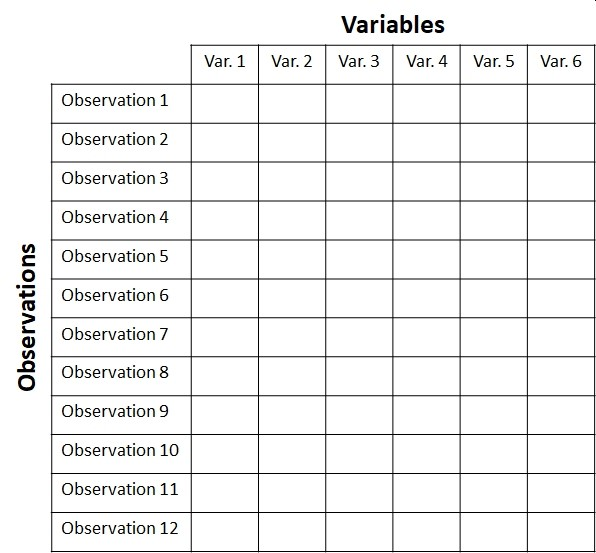
\includegraphics[keepaspectratio,alt={Structure of a typical biological dataset. Observations are stored on rows, and variables that describe those observations are stored in columns. All information about an observation is contained in 1 row. All observations of one variable are contained in 1 column.}]{chapters/../images/review-01.jpg}}\{fig-alt:
``Structure of a typical biological dataset. Observations are stored on
rows, and variables that describe those observations are stored in
columns. All information about an observation is contained in 1 row. All
observations of one variable are contained in 1 column.''\}

\begin{itemize}
\tightlist
\item
  Each row of the dataset is called an \textbf{observation}, or
  sometimes \textbf{record}. Each entity about which data is collected
  corresponds to 1 row of the dataset. For example, the dataset for a
  study of limb morphology in bats might have one row for each species.

  \begin{itemize}
  \tightlist
  \item
    If someone asks what your ``sample size'' or ``number of samples''
    is, the answer is likely the number of rows in your dataset (minus
    any blanks or missing values, of course).
  \end{itemize}
\item
  Each column is called a \textbf{variable}, or sometimes a
  \textbf{feature}.

  \begin{itemize}
  \tightlist
  \item
    Each variable contains 1 and \ul{\textbf{\emph{only}}} 1 kind of
    value. For example, a cell entry like ``12.2 cm'' is not legitimate,
    because it contains 2 kinds of values: a measurement (12.2) and a
    unit (cm). If the units need to be recorded, they should be in a
    separate column.
  \end{itemize}
\end{itemize}

In R, datasets are almost always stored as objects called \textbf{data
frames}. Data frames have rows and columns, and function a bit like a
spreadsheet. Unlike a \textbf{matrix}, rows and columns are not
interchangeable: a row of a data frame is a data frame with 1 row, while
a column is really a vector (i.e., not a data frame).

\pandocbounded{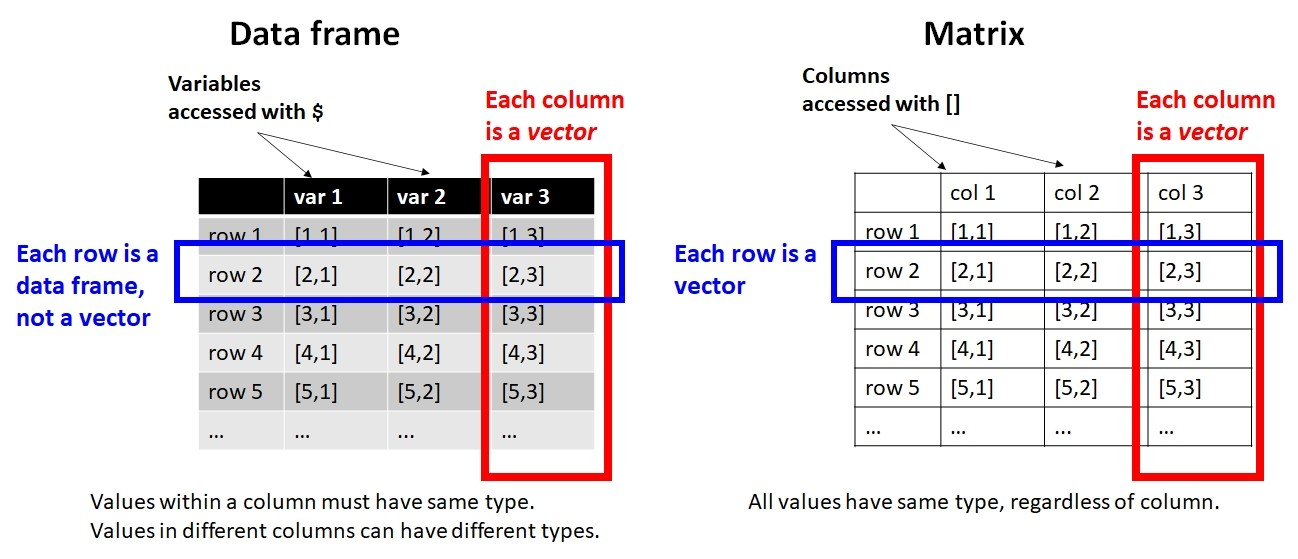
\includegraphics[keepaspectratio,alt={The differences between R data frames (left) and matrices (right).}]{chapters/../images/review-dataframe.jpg}}\{fig-alt:
``\,``\}

Variables in a dataset come in three varieties. Understanding these is
crucial to being able to think about the structure of your dataset and
what kind of statistical test you need.

\begin{itemize}
\tightlist
\item
  \textbf{Response:} outcomes that you want to explain or predict using
  other variables. AKA: dependent variables.
\item
  \textbf{Predictor:} variables that are used to model, or predict,
  response variables. AKA: independent or explanatory variables.
\item
  \textbf{Key:} values which are used to relate 2 or more data tables to
  each other. Fundamental in database design.
\end{itemize}

In this course, every analysis will have have at least 1 response
variable and at least 1 predictor variable. Understanding the nature of
your response variable and predictor variable(s) is key to choosing an
appropriate analysis.

Variables can be either \textbf{categorical} or \textbf{numeric}:

\begin{itemize}
\tightlist
\item
  \textbf{Categorical:} defines group membership; can be encoded as
  numbers, dummy values, or text. Also called \textbf{qualitative}
  variables. E.g., ``control'' vs.~``treated'', ``group 1'' vs.~``group
  2'', ``herbivore'' vs.~``carnivore'', and so on.
\item
  \textbf{Numeric}: numbers. Also called \textbf{quantitative}
  variables. E.g., 1, 2, 3, and so on.
\end{itemize}

When categorical variables are used as explanatory variables, they are
called \textbf{factors}. Each unique value of a factor is called a
\textbf{level}. For example, the factor ``treatment'' might have two
levels, ``control'' and ``exposed''. Or, the factor ``diet'' might have
3 levels: ``herbivore'', ``omnivore'', and ``carnivore''.

Numeric variables can be \textbf{continuous} or \textbf{discrete}:

\begin{itemize}
\tightlist
\item
  \textbf{Continuous} variables can take on any real value within their
  domain. Just because a value is rounded off to integers, does not mean
  they are not continuous. For example, if mice are weighed on a scale
  with precision of 1 g, then all measured weights will be postive whole
  numbers. These should be treated as continuous in the analysis.
\item
  \textbf{Discrete} variables can take on only integer values, and in
  most cases only positive or non-negative integers. Counts are a common
  example of a discrete value.
\end{itemize}

Some kinds of numeric variables need to be treated with care, because
they have a particular domain and set of possible values. Most of these
should probably not be modeled (i.e., treated as the response variable)
using the basic statistical methods in this module. We'll explore models
in \href{@sec-glm1}{Module 18} for these variables.

{\def\LTcaptype{none} % do not increment counter
\begin{longtable}[]{@{}
  >{\raggedright\arraybackslash}p{(\linewidth - 4\tabcolsep) * \real{0.3333}}
  >{\raggedright\arraybackslash}p{(\linewidth - 4\tabcolsep) * \real{0.3333}}
  >{\raggedright\arraybackslash}p{(\linewidth - 4\tabcolsep) * \real{0.3333}}@{}}
\toprule\noalign{}
\begin{minipage}[b]{\linewidth}\raggedright
Type of data
\end{minipage} & \begin{minipage}[b]{\linewidth}\raggedright
Domain
\end{minipage} & \begin{minipage}[b]{\linewidth}\raggedright
How to model
\end{minipage} \\
\midrule\noalign{}
\endhead
\bottomrule\noalign{}
\endlastfoot
Counts & Non-negative integers & GLM or GLMM \\
Proportions & The closed interval \([0,1]\), or possibly the open
interval \((0,1)\) depending on the context & GLM or GLMM; possibly a
\(\chi^2\) test or other test for independence \\
Measurements (mass, length, volume, etc.) & Positive real numbers for
dimensions; real values for temperature (except Kelvin) & Linear model;
transformation or an appropriate GLM/GLMM if needed \\
Censored or truncated data & Usually real numbers with a well-defined
upper or lower limit, often related to limits of detection or
measurement & Special methods such as Tobit models (beyond the scope of
this course\ldots for now) \\
Categorical outcomes & One of a set of possible categories. Categories
may be binary, ordered, or unordered. Although often coded as numbers,
they should not generally be treated as numerical measurements &
Logistic, ordinal, or multinomial regression; GLMMs for non-independent
observations; classification trees (CART) \\
\end{longtable}
}

\section{Frequentist statistics}\label{sec-review-freq}

Classical statistics, such as those taught in introductory statistics or
biostatistics courses, are also \textbf{frequentist} statistics. This
means that these methods rely on probability distributions (also called
frequency distributions) of derived values called \textbf{test
statistics}, and make assumptions about the applicability of those test
statistics. These assumptions can be quite strong, and possibly
restrictive, so you need to be careful when using frequentist tests.

\textbf{If your data do not meet the assumptions of a test, the test
might be invalid.}

The basic procedure of any frequentist test is as follows:

\begin{enumerate}
\def\labelenumi{\arabic{enumi}.}
\tightlist
\item
  Collect data.
\item
  Calculate a summary of the effect size (aka: quantity of interest,
  such as difference in means between groups), which scales the effect
  size by other considerations such as sample size or variability. This
  summary is the \textbf{test statistic}.
\item
  Compare the test statistic to the distribution of test statistics
  expected given the sample size and assuming a true effect size of 0.
  The probability of a test statistic that extreme given a true effect
  size of 0 is the \textbf{\emph{p}-value}.
\item
  If the value of the test statistic is rare enough (i.e., the
  \emph{p}-value is small enough), assume that it was not that large due
  to chance alone, and reject the null hypothesis of no effect. I.e.,
  declare a ``significant'' test result.
\end{enumerate}

Frequentist tests vary widely in their assumptions, the nature of their
test statistics, and so on, but the procedure above describes most of
them.

Another way to think of frequentist statistics is the problem of
distinguishing \textbf{signal} from \textbf{noise}. The biological
patterns we want to discover are the signal. Everything else that we
measure that is influenced by random variation in the subject or the
environment or the measurement process is the noise. Humans are very
good at \href{https://en.wikipedia.org/wiki/Pareidolia}{detecting
patterns in noise}, even if there isn't one.

A real biological pattern should be reliably produce a signal that we
can detect. Noise, on the other hand, can produced apparent signals but
not reliably or repeatedly. Frequentist statistics is a formalized way
of asking the question ``How likely is it that this pattern is due to
noise?''. If the answer is a sufficiently low probability, then the
inference is that the pattern is a signal.

\subsection{\texorpdfstring{\emph{p}-values and
NHST}{p-values and NHST}}\label{mod-09-pvalues}

When scientists design experiments, they are testing one or more
\textbf{hypotheses}: proposed explanations for a phenomenon. Contrary to
popular belief, the statistical analysis of experimental results usually
does not test a researcher's hypotheses directly. Instead, statistical
analysis of experimental results focuses on comparing experimental
results to the results that might have occurred if there was no effect
of the factor under investigation. This paradigm is called \textbf{null
hypothesis significance testing (NHST)} and, for better or worse, is the
bedrock of modern scientific inference.

In other words, traditional statistics sets up the following:

\begin{itemize}
\item
  \textbf{Null hypothesis (\(H_0\)):} default assumption that some
  effect (or quantity, or relationship, etc.) is zero and does not
  affect the experimental results
\item
  \textbf{Alternative hypothesis (\(H_a\) or \(H_1\)):} assumption that
  the null hypothesis is false. Usually this is the researcher's
  scientific hypothesis, or proposed explanation for a phenomenon.
\end{itemize}

In (slightly) more concrete terms, if researchers want to test the
hypothesis that some factor X has an effect on measurement Y, then they
would run an experiment comparing observations of Y across different
values of X. They would then have the following set up:

\begin{itemize}
\item
  \textbf{Null hypothesis:} Factor X does not affect Y.
\item
  \textbf{Alternative hypothesis:} Factor X affects Y.
\end{itemize}

Notice that alternative hypothesis is the \textbf{logical negation} of
the null hypothesis, not a statement about another variable (e.g.,
``Factor Z affects Y''). This is an easy mistake to make and one of the
weaknesses of NHST: the word ``hypothesis'' in the phrase ``null
hypothesis'' is not being used in the sense that scientists usually use
it. This unfortunate choice of vocabulary is responsible for generations
of confusion among researchers and statistics learners.

In order to test an ``alternative hypothesis'', what researchers usually
do is estimate how likely the data would be if the null hypothesis were
true. If a pattern seen in the data is highly unlikely, this is taken as
evidence that the null hypothesis should be rejected in favor of the
alternative hypothesis. This is not the same as ``accepting'' or
``proving'' the alternative hypothesis. Instead, we ``reject'' the null
hypothesis. In the other case, we do not ``accept'' the null hypothesis,
we ``fail to reject'' it.

The null hypothesis is usually translated to a prediction like one of
the following:

\begin{itemize}
\item
  The mean of Y is the same for all levels of X.
\item
  The mean of Y does not differ between observations exposed to X and
  observations not exposed to X.
\item
  Outcome Y is equally likely to occur when X occurs as it is when X
  does not occur.
\item
  Rank order of Y values does not differ between levels of X.
\end{itemize}

All of these predictions have something in common: \textbf{Y is
independent of X}. That's what the null hypothesis means. To test the
predictions of the null hypothesis, we need a way to calculate what the
data might have looked like if the null hypothesis was correct. Once we
calculate that, we can compare the data to those calculations to see how
``unlikely'' the actual data were. Data that are sufficiently unlikely
under the assumption that the null hypothesis is correct---a
``significant difference''---are a kind of evidence that the null
hypothesis is false.

Most classical statistical tests calculate a summary statistic called a
\textbf{\emph{p}-value} to estimate how likely some observed pattern in
the data would be if the null hypothesis was true. This is the value
that researchers often use to make inferences about their data. The
\emph{p}-value depends on many factors, as we'll see, but the most
important are:

\begin{itemize}
\tightlist
\item
  The magnitude of some \textbf{test statistic}: a summary of the
  pattern of interest.
\item
  Sample size, usually expressed as degrees of freedom (DF)
\item
  The variability of the data
\item
  The consistency, sign, and magnitude of the observed pattern
\end{itemize}

When I teach statistics to biology majors, I try to avoid the terms
``null hypothesis'' and ``alternative hypothesis'' at first, because
most of my students find them confusing. Instead, I instruct students to
ask two questions about a hypothesis:

\begin{enumerate}
\def\labelenumi{\arabic{enumi}.}
\item
  What should we observe if the hypothesis is not true?
\item
  What should we observe if the hypothesis is true?
\end{enumerate}

In order to be scientific hypothesis, both of those questions have to be
answerable. Otherwise, we have no way of distinguishing between a
situation where a hypothesis is supported, or a situation where it is
not, because experimental results could always be due to random chance
(even if the probability of that is very small). All we can really do is
estimate how likely it is that random chance drove the outcome.

When interpreting \emph{p}-values, there are \textbf{\emph{3 extremely
important things to remember}}:

\begin{enumerate}
\def\labelenumi{\arabic{enumi}.}
\item
  When \(p<0.05\), the hypothesis is ``supported''. When \(p\ge0.05\),
  the hypothesis is ``not supported''. Notice that the terms are
  ``supported'' or ``not supported''. Words like ``proven'' or
  ``disproven'' are not appropriate when discussing \emph{p}-values.
\item
  The \emph{p}-value is \textbf{\emph{not}} the probability that your
  hypothesis is false, or the probability that a hypothesis is true. It
  is a heuristic for assessing how well data support or do not support a
  hypothesis.
\item
  \emph{p}-values depend on many factors, including sample size, effect
  size, variation in the data, and how well the data fit the assumptions
  of the statistical test used to calculate the \emph{p}-value. This
  means that \emph{p}-values should not be taken at face value and
  \textbf{\emph{never}} used as the sole criterion by which a hypothesis
  is accepted or rejected.
\end{enumerate}

When a statistical test returns a \emph{p}-value less than 0.05, we say
that the results are ``statistically significant'' and we ``reject the
null hypothesis''. For example, a ``statistically significant
difference'' in means between two groups, or a ``statistically
significant correlation'' between two numeric variables.

When a statistical test returns a \emph{p}-value of 0.05 or greater, we
say that the test (or difference, or whatever) is ``not statistically
significant'' and we ``fail to reject the null hypothesis''. Notice that
we do not ``accept the null hypothesis''--that would require a different
kind of analysis.

\section{Alternatives to frequentist statistics}\label{sec-review-alt}

\subsection{Information-theoretic methods}\label{sec-review-alt-it}

One of the main alternatives to NHST is information-theoretic (IT)
modeling. IT methods borrow insights from information theory to draw
conclusions about the extent to which statistical models describe data
(Burnham and Anderson 2002). Rather than evaluating individual
hypotheses primarily using \emph{p}-values, IT methods can be used to
compare different models in terms of how much information is expected to
be lost by using each model to represent the underlying process (Hobbs
and Hilborn 2006). In other words, whereas NHST often asks whether
particular effects are supported by the data, IT methods emphasize
comparing the relative support for entire models.

There are several information criteria in use, but many balance two
components: one representing how well the model fits the observed data,
based on its likelihood, and another that penalizes the model for
complexity (i.e., number of parameters). These information criteria are
used to compare models to each other, not to determine whether any
particular model is ``significant'' or whether any of its terms are
significant. The complexity penalty is important because adding
parameters will generally improve, or at least not worsen, the fit of a
model to the observed data, even when those additional parameters have
little value for describing the underlying process. Without such a
penalty, model selection would therefore tend to favor overly complex
models\ldots a phenomenon called \textbf{overfitting}.

The most common information criterion is Akaike's Information Criterion
(\(AIC\)) (Burnham and Anderson 2002):

\[AIC=-2\log{\left(\hat{L}\right)+2K}\]

where \(\hat{L}\) is the maximum value of the likelihood function and
\(K\) is the number of estimated parameters in the model (e.g., slopes
and intercepts). Lower values of AIC indicate a better balance between
model fit and model complexity. The multiplier of 2 on the \(K\) term is
the penalty for complexity (i.e., adding additional parameters). This
makes adding another parameter supported only if it improves the
likelihood enough to overcome the penalty.

Other information criteria exist, such as the \(AIC\) corrected for
small sample sizes, \(AIC_C\):

\[{AIC}_C=AIC+\frac{2K\left(K+1\right)}{n-K-1}\]

Where \(n\) is the number of observations used to fit the model. The
correction becomes smaller as smaple size increases relative to the
number of parameters, so \(AIC_C\) converges toward \(AIC\) as sample
size increases. Exactly what constitutes a ``small'' sample size is
subjective, but Burnham and Anderson (2002) suggest that \(AIC_C\)
should be used when \(n/K<40\).

Many other information criteria exist, such as \(QAIC\) and \(QAIC_C\)
for use when overdispersion in suspected (Lebreton \emph{et al.} 1992),
Bayesian information criterion (\emph{BIC}) which has a stronger
complexity penalty; and deviance information criterion (\emph{DIC})
which is often used in Bayesian inference.

\subsubsection{Likelihood?}\label{likelihood}

Before we jump into an example IT data analysis, we also need to
understand the concept of the \textbf{likelihood function}. A likelihood
function describes how well different possible parameter values are
supported by the observed data under a particular statistical model. A
statistical model specifies the mathematical relationships among
variables and the probability distribution of the observations; examples
include a linear regression model or a Poisson GLM.

In symbols, we can write the likelihood function as:

\[\mathcal{L}\left(\theta|x\right)\]

where \(x\) represents the observed data and \(\theta\) represents one
or more unobserved parameters. For the data we actually observed, the
likelihood function asks: which possible values of \(\theta\) would make
these data more or less plausible?

Importantly, likelihood is \textbf{\emph{not}} the probability that a
particular parameter value or model is correct. Although
\(\mathcal{L}\left(\theta|x\right)\) is written with the parameters to
the left of the vertical bar, it is based on the probability of the data
given the parameters, \(p\left(x|\theta\right)\), not the probability of
the parameters given the data, \(p\left(\theta|x\right)\). The latter is
a Bayesian posterior probability (see
Section~\ref{sec-review-alt-bayes}).

The takeaway is that probability askes about data when the model is
known, while likelihood asks about parameter values after the data have
been observed.

Likelihoods are most famously used in modern data analysis as
\textbf{maximum likelihood explanation (MLE)}. This procedure attempts
to estimate the parameters of a model most likely to produce the
observed data.

Here's a quick example: imagine you have measured 5 squirrel femurs and
found lengths of 63.6, 66.5, 64.2, 67.6, and 68.3 mm, yielding an
observed sample mean and SD of \(66.0\pm2.1\) mm. What estimate of the
population mean \(\mu\) that makes this set of measurements most
plausible?

\begin{Shaded}
\begin{Highlighting}[]
\NormalTok{a }\OtherTok{\textless{}{-}} \FunctionTok{c}\NormalTok{(}\FloatTok{63.6}\NormalTok{, }\FloatTok{66.5}\NormalTok{, }\FloatTok{64.2}\NormalTok{, }\FloatTok{67.6}\NormalTok{, }\FloatTok{68.3}\NormalTok{)}
\FunctionTok{mean}\NormalTok{(a)}
\end{Highlighting}
\end{Shaded}

\begin{verbatim}
[1] 66.04
\end{verbatim}

\begin{Shaded}
\begin{Highlighting}[]
\FunctionTok{sd}\NormalTok{(a)}
\end{Highlighting}
\end{Shaded}

\begin{verbatim}
[1] 2.067124
\end{verbatim}

Consider 3 candidates for \(\mu\): 64, 66, and 68. For any proposed
value of \(\mu\), \texttt{dnorm()} tells us the probability density of
observing each femur length under a normal distribution with that mean:

\begin{Shaded}
\begin{Highlighting}[]
\NormalTok{samp.sd }\OtherTok{\textless{}{-}} \FloatTok{2.1}
\FunctionTok{dnorm}\NormalTok{(a, }\AttributeTok{mean=}\DecValTok{64}\NormalTok{, }\AttributeTok{sd=}\NormalTok{samp.sd)}
\end{Highlighting}
\end{Shaded}

\begin{verbatim}
[1] 0.18655737 0.09352817 0.18911291 0.04370627 0.02334791
\end{verbatim}

\begin{Shaded}
\begin{Highlighting}[]
\FunctionTok{dnorm}\NormalTok{(a, }\AttributeTok{mean=}\DecValTok{66}\NormalTok{, }\AttributeTok{sd=}\NormalTok{samp.sd)}
\end{Highlighting}
\end{Shaded}

\begin{verbatim}
[1] 0.09887122 0.18466340 0.13156914 0.14211406 0.10428277
\end{verbatim}

\begin{Shaded}
\begin{Highlighting}[]
\FunctionTok{dnorm}\NormalTok{(a, }\AttributeTok{mean=}\DecValTok{68}\NormalTok{, }\AttributeTok{sd=}\NormalTok{samp.sd)}
\end{Highlighting}
\end{Shaded}

\begin{verbatim}
[1] 0.02115483 0.14719781 0.03695464 0.18655737 0.18804388
\end{verbatim}

Because we observed more than 1 measurement, and assume that they are
independent, the joint likelihood is the product of their densities:

\begin{Shaded}
\begin{Highlighting}[]
\FunctionTok{prod}\NormalTok{(}\FunctionTok{dnorm}\NormalTok{(a, }\AttributeTok{mean=}\DecValTok{64}\NormalTok{, }\AttributeTok{sd=}\NormalTok{samp.sd))}
\end{Highlighting}
\end{Shaded}

\begin{verbatim}
[1] 3.367191e-06
\end{verbatim}

\begin{Shaded}
\begin{Highlighting}[]
\FunctionTok{prod}\NormalTok{(}\FunctionTok{dnorm}\NormalTok{(a, }\AttributeTok{mean=}\DecValTok{66}\NormalTok{, }\AttributeTok{sd=}\NormalTok{samp.sd))}
\end{Highlighting}
\end{Shaded}

\begin{verbatim}
[1] 3.560036e-05
\end{verbatim}

\begin{Shaded}
\begin{Highlighting}[]
\FunctionTok{prod}\NormalTok{(}\FunctionTok{dnorm}\NormalTok{(a, }\AttributeTok{mean=}\DecValTok{68}\NormalTok{, }\AttributeTok{sd=}\NormalTok{samp.sd))}
\end{Highlighting}
\end{Shaded}

\begin{verbatim}
[1] 4.036932e-06
\end{verbatim}

It looks like 66 has the greatest joint likelihood across all observed
data. But we can get a fuller picture if we test more values:

\begin{Shaded}
\begin{Highlighting}[]
\CommentTok{\# series of possible mu to test}
\NormalTok{test.mu }\OtherTok{\textless{}{-}} \FunctionTok{seq}\NormalTok{(}\DecValTok{60}\NormalTok{, }\DecValTok{72}\NormalTok{, }\AttributeTok{by=}\FloatTok{0.01}\NormalTok{)}

\CommentTok{\# number of possible mu}
\NormalTok{n }\OtherTok{\textless{}{-}} \FunctionTok{length}\NormalTok{(test.mu)}

\CommentTok{\# set up vector to hold likelihood}
\CommentTok{\# function of each candidate mu}
\NormalTok{lik }\OtherTok{\textless{}{-}} \FunctionTok{numeric}\NormalTok{(n)}

\CommentTok{\# calculate likelihoods of mu\textquotesingle{}s in a loop}
\ControlFlowTok{for}\NormalTok{(i }\ControlFlowTok{in} \DecValTok{1}\SpecialCharTok{:}\NormalTok{n)\{lik[i] }\OtherTok{\textless{}{-}} \FunctionTok{prod}\NormalTok{(}\FunctionTok{dnorm}\NormalTok{(a, test.mu[i], }\AttributeTok{sd=}\NormalTok{samp.sd))\}}\CommentTok{\#i}

\CommentTok{\# now plot the likelihood function vs. mu}
\FunctionTok{plot}\NormalTok{(test.mu, lik, }\AttributeTok{type=}\StringTok{"l"}\NormalTok{, }\AttributeTok{lwd=}\DecValTok{3}\NormalTok{,}
     \AttributeTok{xlab=}\FunctionTok{expression}\NormalTok{(mu),}
     \AttributeTok{ylab=}\StringTok{"Likelihood"}\NormalTok{)}
\FunctionTok{abline}\NormalTok{(}\AttributeTok{v=}\FunctionTok{mean}\NormalTok{(a), }\AttributeTok{lwd=}\DecValTok{2}\NormalTok{, }\AttributeTok{lty=}\DecValTok{2}\NormalTok{, }\AttributeTok{col=}\StringTok{"red"}\NormalTok{)}
\FunctionTok{text}\NormalTok{(}\FloatTok{66.2}\NormalTok{, }\FloatTok{0.5e{-}5}\NormalTok{, }\FunctionTok{expression}\NormalTok{(}\FunctionTok{bar}\NormalTok{(x)}\SpecialCharTok{==}\FloatTok{66.04}\NormalTok{), }\AttributeTok{adj=}\DecValTok{0}\NormalTok{, }\AttributeTok{col=}\StringTok{"red"}\NormalTok{)}
\FunctionTok{abline}\NormalTok{(}\AttributeTok{h=}\NormalTok{lik[}\FunctionTok{which.max}\NormalTok{(lik)], }\AttributeTok{lty=}\DecValTok{2}\NormalTok{, }\AttributeTok{lwd=}\DecValTok{2}\NormalTok{, }\AttributeTok{col=}\StringTok{"blue"}\NormalTok{)}
\FunctionTok{text}\NormalTok{(}\FloatTok{67.5}\NormalTok{, }\FloatTok{3.4e{-}5}\NormalTok{, }\FunctionTok{expression}\NormalTok{(}\FunctionTok{hat}\NormalTok{(mu)}\SpecialCharTok{==}\FloatTok{66.04}\NormalTok{), }\AttributeTok{adj=}\DecValTok{0}\NormalTok{, }\AttributeTok{col=}\StringTok{"blue"}\NormalTok{)}
\end{Highlighting}
\end{Shaded}

\pandocbounded{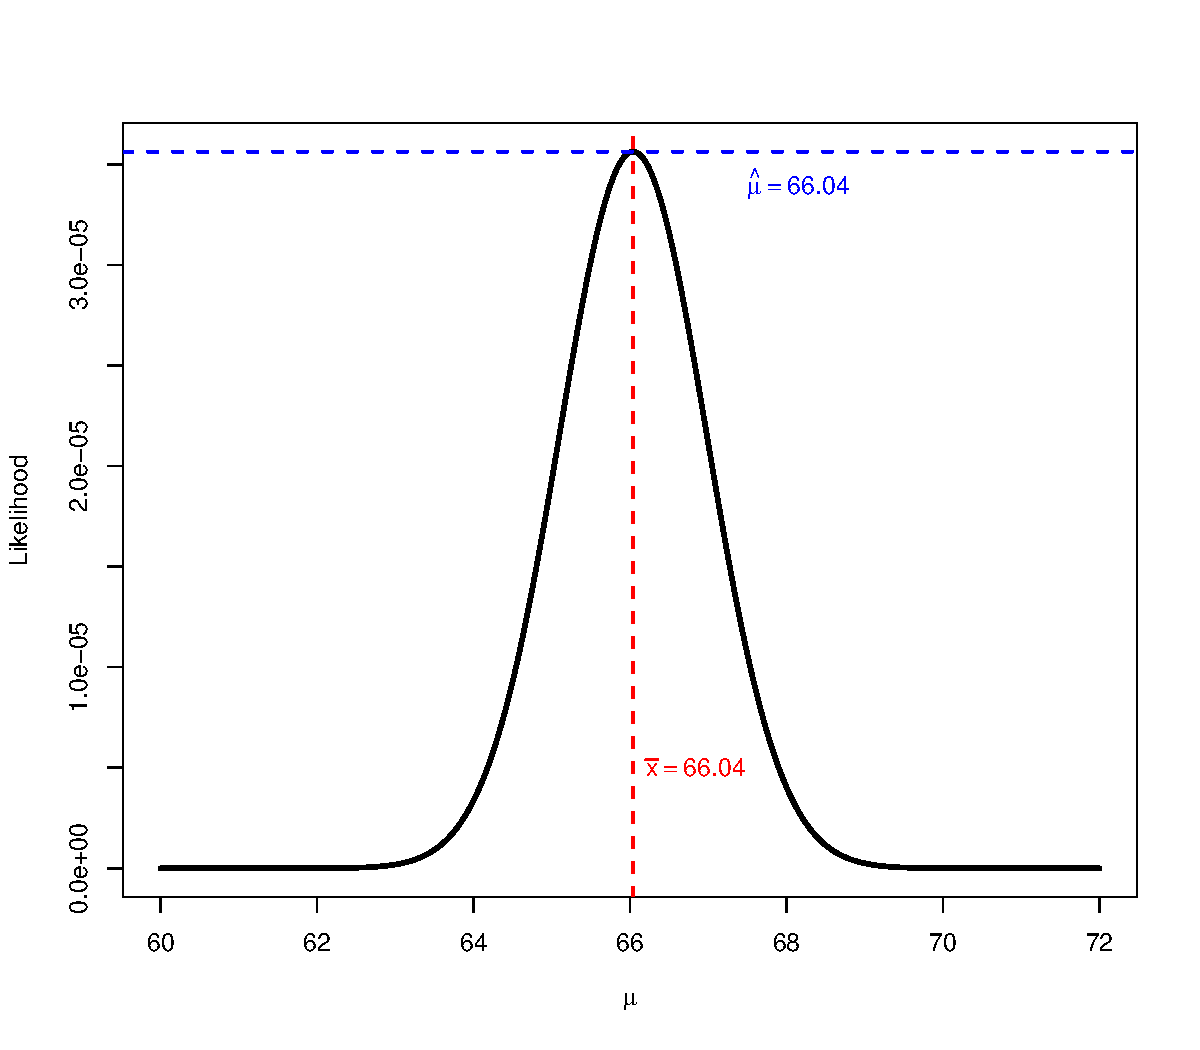
\includegraphics[keepaspectratio]{chapters/ch14_files/figure-pdf/unnamed-chunk-9-1.pdf}}

In this case, the sample mean \(\bar{x}=66.04\) (\texttt{mean(a)}) is
the same as the \(\mu\) value that maximized the joint likelihood of the
5 observed values, \(\hat{\mu}=66.04\)
(\texttt{test.mu{[}which.max(lik){]}}). But, the code above only worked
because we held the SD to be known and the same as the sample SD. If we
didn't, we would have to search over a range of possible SD values, and
find the combination of \(\hat{\mu}\) and \(\hat{\sigma}\) that
maximized the likelihood. In that case, the profile of likelihoods would
have been a surface, not a line. The maximum likelihood estimates for
something like a linear regression model, or a Poisson GLM, are found by
similar procedure, only with multiple parameters making the profiling
much more complicated.

\subsection{Bayesian inference}\label{sec-review-alt-bayes}

\textbf{Bayesian inference} is a framework for evaluating evidence and
\emph{updating beliefs based on evidence}. When conducting Bayesian
inference, researchers start with some initial idea about their model
system: a \textbf{prior}. They then collect evidence (data), and update
their idea based on the evidence. The updated idea is called the
\textbf{posterior}.

\begin{itemize}
\tightlist
\item
  When the prior is strong, or the evidence weak, their ideas will not
  be updated much and the posterior will be strongly influenced by the
  prior.
\item
  When the evidence is strong, or the prior weak, the posterior will be
  updated more and thus less influenced by the prior.
\end{itemize}

Some researchers prefer to use naïve or uninformative priors, so that
their conclusions are influenced mostly by the evidence. Bayesian
statistical methods will return essentially the same parameter estimates
(e.g., differences in means or slopes) as other methods when
uninformative priors are used. This means that almost any traditional
statistical analysis can be replaced with an equivalent Bayesian one.
The statistical models that are fit, such as linear regression or ANOVA,
are the same. All that really changes is how the researcher interprets
the relationship between the model and the data.

In frequentist inference, researchers consider parameters like slopes,
intercepts, effect sizes, etc., as fixed, unknown parameters and
consider the data to occur stochastically following probability
distributions. Bayesian inference flips that script, treating the data
as fixed, and assuming that the model parameters are unknown quantities
following probability distributions.

Bayesian inference depends on \textbf{Bayes' theorem}:

\[p\left(H|E\right)=\frac{P\left(E|H\right)P\left(H\right)}{P\left(H\right)P\left(E|H\right)+P\left(\lnot H\right)P\left(E|\lnot H\right)}=\frac{P\left(E|H\right)P\left(H\right)}{P\left(E\right)}\]

where

\begin{itemize}
\tightlist
\item
  \(H\) is a hypothesis that can be true or false
\item
  \(p\left(H\right)\) is the prior, an estimate of the probability of
  the hypothesis being true before any new data (\(E\)) are observed
\item
  \(E\) is evidence, specifically new data used to update the prior
\item
  \(p\left(H|E\right)\) is the probability of \(H\) given \(E\). I.e.,
  the probability of the hypothesis being true after new evidence is
  observed. This is also called the \textbf{posterior probability}.
\item
  \(p\left(E\right)\) is the probability of \(E\) regardless of \(H\).
  I.e., the probability of observing the evidence whether or not the
  hypothesis is true. \(p\left(E\right)\) is called the \textbf{marginal
  likelihood}.
\item
  \(p\left(E|H\right)\) is the probability of observing the evidence
  \(E\) given \(H\). I.e., the probability of observing the evidence if
  the hypothesis is true. \(p\left(E|H\right)\) is also called the
  \textbf{likelihood}.
\end{itemize}

Bayes' theorem is powerful because it is very general. The precise
nature of \(E\) and \(H\) do not matter. All that matters is that one
could sensibly define an experiment or set of observations in which
\(E\)* might depend on \(H\) and vice versa.

Bayesian inference is attractive to many biologists because it mimics
the way that scientists actually think: starting with one idea (a
prior), collecting evidence, then updating that idea (posterior). Part
of the Bayesian calculation is \(p\left(H|E\right)\), or the probability
of the hypothesis being true given the evidence that is observed.
Contrast this with the frequentist \emph{p}-value, which is
\(p\left(E|\lnot H\right)\). Most people instinctively want the first,
but have to settle with the almost backwards logic of the
\emph{p}-value.

Here is a quick example of Bayesian reasoning. Imagine you go to the
doctor and get tested for a rare condition,
\href{https://medlineplus.gov/genetics/condition/niemann-pick-disease/}{Niemann-Pick
disease}. Your doctor tells you that this disease affects about 1 in
250000 people. Unfortunately, you test positive. But, the doctor tells
you not to worry because the test is only 99\% reliable. Why is the
doctor so sanguine, and what is the probability that you have
Niemann-Pick disease?

The probability of having this disease can be estimated using Bayes'
theorem. First, use what you know to assemble the terms:

\begin{itemize}
\tightlist
\item
  The overall incidence is 1 in 250000 people, or 0.0004\%. So, the
  prior probability \(P\left(H\right)\) is 0.000004.
\item
  The probability of a positive test given that you have the disease,
  \(P\left(E|H\right)\), is 0.99 because the test is 99\% reliable.
\item
  The denominator, \(P\left(E\right)\), is the unconditional probability
  of a positive test.
\end{itemize}

The denominator includes two possibilities: either a positive test when
someone has the disease, or a positive test when someone doesn't have
the disease. That is, the probability of a true positive \emph{or} a
false positive. This can be calculated as:

\[p\left(H\right)\left(E|H\right)+p\left(\lnot H\right)p\left(E|\lnot H\right)\].

The first term is the probability of a true positive
(\(p\left(E|H\right)\)) scaled by the probability of having the disease
(\(p\left(H\right)\)). The second is the probability of a false positive
(\(p\left(E|\lnot H\right)\)) scaled by the probability of not having
the disease (\(p\left(\lnot H\right)\)). We can simplify a bit by
reasoning that \(p\left(\lnot H\right)\) is really
\(1-p\left(H\right)\).

Plug every thing into Bayes' rule:

\[p\left(H|E\right)=\frac{P\left(E|H\right)P\left(H\right)}{P\left(H\right)P\left(E|H\right)+\left(1-P\left(H\right)\right)P\left(E|\lnot H\right)}=p\left(H|E\right)=\frac{\left(0.99\right)\left(0.000004\right)}{\left(0.000004\right)\left(0.99\right)+\left(0.999996\right)\left(0.01\right)}\]
and simplify:

\[p\left(H|E\right)=\frac{0.00000396}{0.01000392}=0.000396\]

That's not very worrying! In this example, the test evidence can't
overcome the fact that the disease is so rare. In other words, even
among people who get a positive test, it's far more likely that you
don't have the disease but got a false positive than that you have the
disease and got a true positive. This is an example of a very strong
prior being more influential than the evidence.

There's an issue with this calculation, though. The prior probability of
0.000004 was based on the assumption that the test was conducted on a
random person from the population. Do physicians conduct tests for
vanishingly rare diseases on random people? Of course not. Maybe this
physician only orders this test if they think that there is a 10\%
chance that you really have the disease. This might be because, in their
experience, 10\% of people with your symptoms turn out to have the
disease. In that case, the calculation becomes:

\[\left(H|E\right)=\frac{\left(0.99\right)\left(0.1\right)}{\left(0.1\right)\left(0.99\right)+\left(0.9\right)\left(0.01\right)}\]

which simplifies to:

\[p\left(H|E\right)=\frac{0.099}{0.108}=0.916\]

91.6\% is a lot more worrying than 0.0004\%. This example shows that the
prior probability can have a huge effect on the posterior probability.

One way to visualize Bayes' rule is to think of the entire probability
space as occupying a square with area 1. The square has 4 sections:

\begin{figure}[H]

\caption{Bayes theorem helps us reason about the relative probabilities
of observing a piece of evidence E or not when a hypothesis H is true or
not true. The area of all four sections must add up to 1. According to
Bayes' theorem, the probability of a hypothesis H being true, given
evidence E, is the ratio of \(P\left(E|H\right)\) to
\(P\left(E|H\right)+P\left(E|lnot H\right)\).}

{\centering \pandocbounded{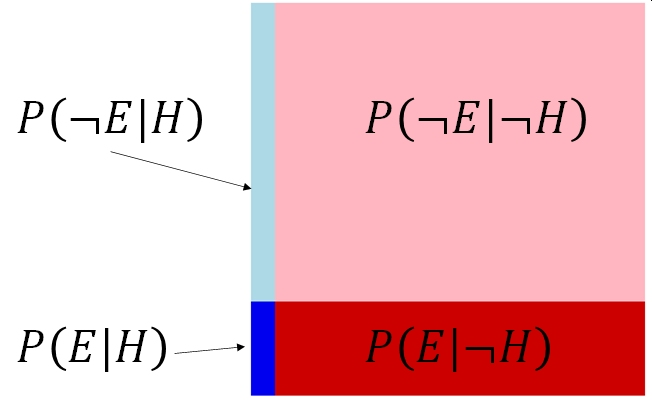
\includegraphics[keepaspectratio]{chapters/../images/review-bayes1.jpg}}

}

\end{figure}%

Notice that the prior probability \(p\left(H\right)\) (the two left,
blue sections) is much smaller than the probability of \(\lnot H\).
Bayes' rule restricts our focus to the cases where we observe the
evidence--the bottom two sections. Given that the evidence was observed,
the sections with \(\lnot E\) are irrelevant. The calculation then
becomes:

\pandocbounded{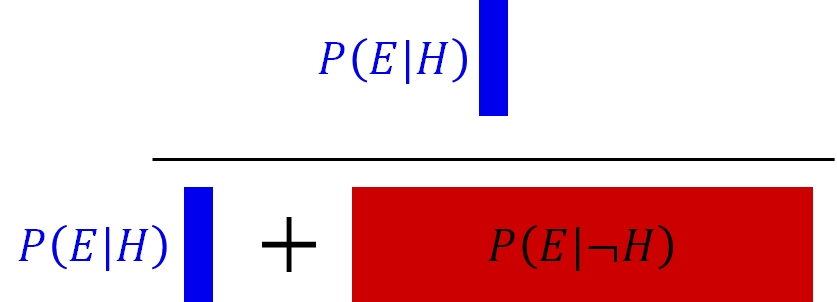
\includegraphics[keepaspectratio,alt={In Bayesian inference, the probability of the hypothesis being true given the observed evidence is the ratio of cases where the evidence is observed and the hypothesis is true, to all cases where the evidence is observed.}]{chapters/../images/review-bayes2.jpg}}
Besides its epistemological neatness, another advantage of Bayesian
inference in practice is that parameters in Bayesian models (e.g,
slopes, intercepts, etc.) are estimated with \textbf{credible intervals
(CRI)}, not \textbf{confidence intervals (CI)}.

\begin{itemize}
\tightlist
\item
  A frequentist 95\% confidence interval is a statement about the long
  run performance of a series of repeated experiments. If we repeatedly
  collected new samples and calculated intervals the same way, about
  95\% of those intervals would contain the true parameter. This is not
  the same as saying that there is a 95\% probability that the true
  parameter value lies within out estimated CI.
\item
  A Bayesian 95\% credible interval is a statement about the parameter
  itself. Given the data, model, and prior, there is a 95\% probability
  that the parameter lies within the interval. That is, a credible
  interval does what most people mistakenly think the confidence
  interval does!
\end{itemize}

I'm a big fan of Bayesian inference. But, I'll admit that there is a
downside: Bayesian model-fitting is not available in base R, and
requires specialized packages and sometimes external software. Should
you go through all of this Bayesian trouble? There are a few reasons
where Bayesian inference might be preferable to traditional frequentist
statistics.

\begin{enumerate}
\def\labelenumi{\arabic{enumi}.}
\tightlist
\item
  The model to be fit is very complex. Because the user can specify any
  model they want, they can fit any model they want.
\item
  Maximum-likelihood methods often require explicit derivations of model
  likelihoods, whereas an MCMC approach does not (MCMC, or Markov-chain
  Monte Carlo, is a common method for fitting Bayesian models). This
  means that models whose likelihoods have no closed form solution, or
  have computationally difficult solutions, can be estimated more easily
  with Bayesian methods than maximum likelihood (sometimes).
\item
  The researcher has prior information that they would like to
  incorporate into the analysis. This can reduce the amount of data
  needed to reach certain conclusions.
\item
  Maximum likelihood methods are not effective in some situations.
\item
  Error propagation is very easy under Bayesian inference (especially
  MCMC).
\item
  The researcher prefers the philosophy of Bayesian inference.
\end{enumerate}

Bayesian inference is beyond the scope of this course, but if you're
interested head on over to my course notes for \href{}{BIOL 7950:
Bayesian Inference for Biologists}.

\section{Linear models}\label{sec-review-lin}

\subsection{What is ``linear''?}\label{sec-review-lin-def}

\textbf{Linear models} are called \emph{linear} models because they can
be expressed as \textbf{linear combinations} of a set of estimated
parameters. A linear combination is an expression formed by multiplying
each term by a constant, and adding the products together. For example,

\[ax+by\]

is a linear combination of \(x\) and \(y\), where \(a\) and \(b\) are
constants. The \(x\) and the \(y\) could be single values, or, as
commonly used in statistics, \textbf{vectors} of values. A vector in
this sense is an ordered set of values. One example of a linear
combination that you're already familiar with is a
\href{sec-desc-cen-mean-wm}{weighted mean}. The weighted mean of a set
of numbers \(\left[x_1,x_2,\ldots,x_n\right]\) is given by the sum

\[\bar{x}_w=\sum_i^n\left(\frac{w_i}{\sum_i^nw_i}\right)x_i\]

Because the sum of all weights must be 1, this simplifies to:

\[\bar{x}_w=\sum_i^n\left(w_i\right)x_i\]

meaning that the weights are the coefficients, and the values of \(x\)
are the terms. Actually, the mean itself is a linear combination, where
all weights are equal to \(1/n\).

To generalize, a linear model consists of the sum of the products of an
input vector and a series of coefficients of the same length. In a
simple linear regression, the coefficient is the slope: the expected
change in \(Y\) associated with a unit increase in \(X\).

Importantly, a linear model must be \emph{linear in its parameters}, not
necessarily in the predictor variables themselves. For example, the
model \(y=\beta_0+\beta_1x+\beta_2x^2\) is nonlinear in \(x\) because
the \(x^2\) forces a curved graph. But, if \(x^2\) increases by 1, then
\(y\) will increase by \(\beta_2\). This is what it means to be ``linear
in its parameters''.

All linear models can be written very compactly in matrix notation:

\[
\mathbf{Y}=\mathbf{X}\boldsymbol{\beta}+\boldsymbol{\varepsilon}
\]

The boldface variables indicate that each term is a matrix or a vector,
not a variable in the usual sense. In most biological analyses,
\(\mathbf{Y}\), \(\mathbf{\beta}\), and \(\mathbf{\varepsilon}\) are
column vectors, which are like matrices with 1 column. The matrix
\(\mathbf{X}\) is the \textbf{design matrix}, which contains the values
of the explanatory variables used to fit the model.

The notation above may be compact, but expanding everything out makes it
clearer what is going on:

\[
\left[
\begin{matrix}
y_1 \\
y_2 \\
\vdots \\
y_n
\end{matrix}
\right]
=
\left[
\begin{matrix}
1 & x_{11} & \cdots & x_{1p} \\
1 & x_{21} & \cdots & x_{2p} \\
\vdots & \vdots & \ddots & \vdots \\
1 & x_{n1} & \cdots & x_{np}
\end{matrix}
\right]
\left[
\begin{matrix}
\beta_0 \\
\beta_1 \\
\vdots \\
\beta_p
\end{matrix}
\right]
+
\left[
\begin{matrix}
\varepsilon_1 \\
\varepsilon_2 \\
\vdots \\
\varepsilon_n
\end{matrix}
\right]
\]

where \(n\) is the number of observations, and \(p\) is the number of
predictors. The leftmost column in \(\mathbf{X}\), consisting of all 1s,
are what gets multiplied by \(\beta_0\) to produce the intercept. For
example, the expected value for the first value of the response \(y_1\)
is equal to:

\[E\left(y_1\right)=\beta_0\left(1\right)+\beta_1\left(x_{11}\right)+\beta_2\left(x_{12}\right)+\ldots+\beta_p\left(x_{1p}\right)\]

where \(x_{ij}\) is the \(x\) value for observation \(i\), predictor
variable \(j\). The observed value of \(y_i\) the expected value plus
some random deviation \(\varepsilon_i\), which comes from a normal
distribution with mean 0 and SD \(\sigma_{res}\) (``res'' is for
``residual'').

\subsubsection{Factors in linear models}\label{factors-in-linear-models}

This notion of linearity is what makes many analyses with
\textbf{factors} (categories or grouping variables) as predictors
``linear''. For example, the \emph{t}-test is a linear model, but it
doesn't really describe a line on a plot of \emph{y} vs.~\emph{x} the
way that linear regression does. However, if you encode the factor
(grouping variable) it should be clear what the difference in group
means really means:

\[
E\left(y_i\right)=\left(1\times\beta_0\right)+\left(x_i\times\beta_1\right)
\]

For group 1, \(x_1=0\), so the expected value is \(\beta_0\). For group
2, \(x_i=1\), so the \(\beta_1\) term comes into play as the difference
in means between groups 1 and 2. This is what R, SAS, and other programs
are doing internally when you analyze data with a factor variable. Here
is what that looks like visually:

\pandocbounded{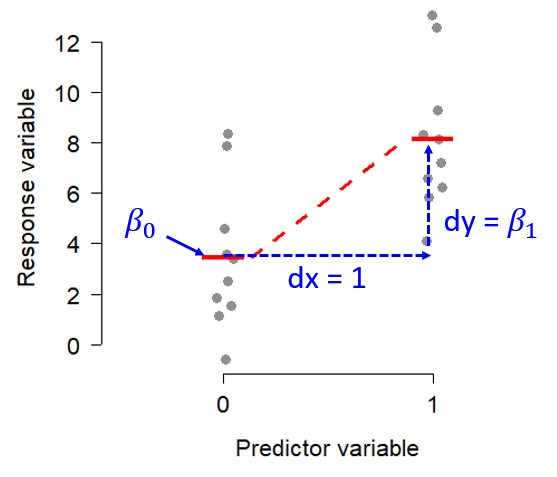
\includegraphics[keepaspectratio,alt={Illustration of how a t-test qualifies as a linear model.}]{chapters/../images/review-ttest.jpg}}
Similarly, a one-way ANOVA with 3 levels can be thought of this way:

\[
E\left(y_i\right)=\left(1\times\beta_0\right)+\left(x_{1,i}\times\beta_1\right)+\left(x_{2,i}\times\beta_2\right)
\]

And visualized this way:

\begin{figure}[H]

\caption{Illustration of how a one-way ANOVA with 3 levels qualifies as
a linear model.}

{\centering \pandocbounded{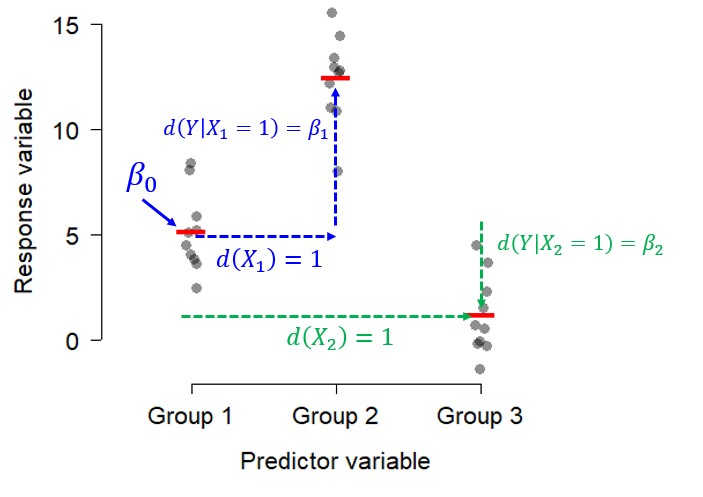
\includegraphics[keepaspectratio]{chapters/../images/review-3anova.jpg}}

}

\end{figure}%

\subsubsection{Linear models and sums of
squares}\label{sec-review-lin-ss}

There are tangible and intangible benefits to using linear models.
First, as shown above, linear models can be written very compactly in
the language of linear algebra (i.e., the branch of mathematics that
deals with certain types of operations on matrices and vectors). From a
practical standpoint, this forces us to organize our datasets sensibly,
into matrices with rows that describe observations and columns that
describe variables. From a computational standpoint, this makes the
computer's job much more efficient because of the architecture of modern
computers.

Second, and less obvious, is that the model coefficients of a linear
model can be \textbf{solved for}, rather than approximated. When we fit
a linear model to data, we are really after the values in the
coefficients matrix. A modern statistical program can solve for these
values rather than having to estimate them. For example, a simple linear
regression with 1 predictor variable \(X\) can be solved by finding the
intercept \(\beta_0\) and \(\beta_1\) that together minimize the sum of
squared residuals \(SS_{res}\). These coefficients are:

\[
{\hat{\beta}}_1=\frac{\sum_{i=1}^{n}\left(x_i-\bar{x}\right)\left(y_i-\bar{y}\right)}{\sum_{i=1}^{n}\left(x_i-\bar{x}\right)^2}
\]

to yield the effect of \(x_1\), \(\beta_1\). The intercept is then:

\[
{\hat{\beta}}_0=\bar{y}-{\hat{\beta}}_1\bar{x}
\]

The caret symbol \(\hat{}\) indicates that a value is an ``estimate'',
even when it is solved for from data (e.g., \(\hat{\beta_1}\) is
pronounced ``beta-one-hat'' and is the estimated slope). Similarly, the
bar above a letter indicates the sample mean (e.g., \(\bar{x}\)'' is
pronounced ``x bar'' and is the mean of all observed \emph{x}).

\subsubsection{Assumptions of linear models}\label{sec-review-lin-assum}

Linear models have some other features and assumptions that you need to
be aware of. If your data or variables violate the assumptions below,
you may need to use something other than linear models to analyze your
data.

\paragraph{Assumption 1: Normal
residuals}\label{assumption-1-normal-residuals}

The linear model assumes that model residuals, the random errors
representing the differences between observed and predicted values,
follow a normal distribution. Models for data that do not have normal
residuals exist, but they are not linear models. We'll explore those in
Chapter~\ref{sec-glm1}.

The assumption of normal residuals explains the last term in the linear
model equation, \(\varepsilon_i\):

\[
y_i=\beta_0+\beta_1x_i+\varepsilon_i
\]

In this equation, \(y_i\) is observation \emph{i} of the response
variable \emph{y}; \(\beta_0\) is the intercept; \(\beta_1\) is the
slope; \(x_i\) is the predictor variable \emph{x} for observation
\emph{i}, and \(\varepsilon_i\) is the residual for observation \emph{i}
(\(\varepsilon\) is the Greek letter ``epsilon'' and usually stands for
error or residual terms). The residual term can be expanded like this:

\[y_i=\beta_0+\beta_1x_i+Normal\left(0,\sigma_{res}\right)\]

This expansion makes it clear that each residual \(\varepsilon_i\) comes
independently from a normal distribution with mean 0 and standard
deviation (SD) \(\sigma_{res}\). For convenience, we sometimes separate
the deterministic part and the stochastic part of the model and write
the \textbf{state space} form of the linear regression model:

\[
y_i\sim Normal\left(\eta_i,\ \sigma_{res}\right)
\]

\[
\eta_i=\beta_0+\beta_1x_i
\]

In this version, the symbol \(\sim\) means ``distributed as'' and
denotes a \textbf{stochastic} relationship---a relationship that
contains some element of randomness. This is in contrast to a
\textbf{deterministic} relationship, which does not (equality, aka:
identity, = is the most famous kind of deterministic relationship).

\paragraph{Assumption 2: Homogeneity of
variance}\label{assumption-2-homogeneity-of-variance}

Linear models assume \textbf{homoscedasticity}, or constant variance.
This means that the residual variance does not depend on either \emph{x}
or \emph{y}.If the variance in the response variable depends on some
predictor variable, then this should be incorporated into the model
(resulting in something other thana linear model). If the variance
appears to depend on the response variable, then there is probably an
issue with the assumed response distribution.

The figure below shows two datasets with a linear relationship between
\emph{x} and \emph{y}. In the left panel, the variance is the same
everywhere (homoscedastic). The right panel shows a heteroscedastic
relationship where the variance increases at larger \emph{x}.

\begin{figure}[H]

\caption{Example of heteroscedasticity, or unequal variance, across the
domain of \(x\). The left panel shows homoscedasticity, where residual
varincee is approximately the same for all \(x\). The right panel shows
heteroscedasticity, where residual variance increases with \(x\)}

{\centering \pandocbounded{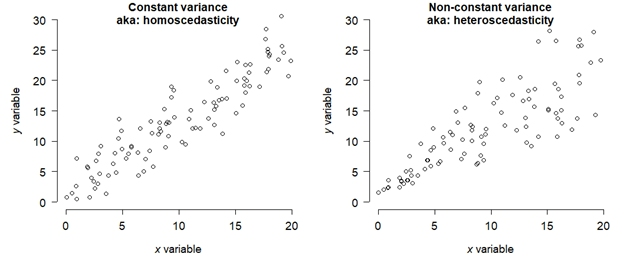
\includegraphics[keepaspectratio]{chapters/../images/review-homog.jpg}}

}

\end{figure}%

The figure below shows two datasets with a categorical predictor,
suitable for a \emph{t}-test. The left panel shows a relationship with
equal variances in each group, while the right panel shows a situation
with unequal variances.

\begin{figure}[H]

\caption{Example of heteroscedasticity, or unequal variance, between two
levels \emph{a} and \emph{b} of some factor. The left panel shows
homoscedasticity, where residual varincee is approximately the same in
group \emph{a} and group \emph{b}. The right panel shows
heteroscedasticity, where residual variance is different in each group.}

{\centering \pandocbounded{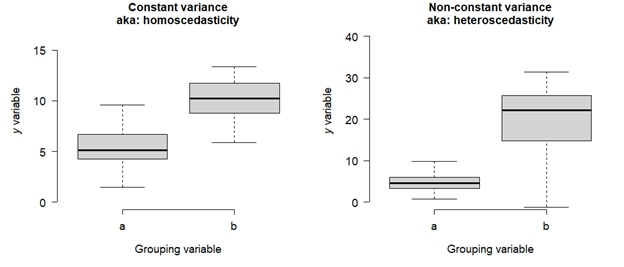
\includegraphics[keepaspectratio]{chapters/../images/review-homog2.jpg}}

}

\end{figure}%

Heteroscedasticity is a serious problem for linear models because it
leads to biased parameter estimates and standard errors (SE) of those
estimates. The latter issue means that significance tests on parameters
will be incorrect. Bayesian statistics does not involve significance
tests, but heteroscedasticity that is unaccounted for will still lead to
biased estimates. The usual solution is to either apply a
variance-stabilizing transformation (like the log-transform),
incorporate variance parameters that can be estimated, or be clever
about choosing a response distribution.

\paragraph{Assumption 3: Fixed and independent
predictors}\label{assumption-3-fixed-and-independent-predictors}

Linear models assume that predictor values are precisely known
(``fixed'') and independent of each other. If there is uncertainty in
the predictor variables, this adds uncertainty to the response values
that linear models cannot account for. Simply put, linear models have a
term for uncertainty in \emph{y}, \(\sigma_{res}\), but no term for
uncertainty in \emph{x}.

\paragraph{Assumption 4: Independently and identically distributed
errors}\label{assumption-4-independently-and-identically-distributed-errors}

(\emph{i}.\emph{i}.\emph{d}.)

The assumption of independently and identically distributed
(\emph{i.i.d.}) errors is \textbf{\emph{very}} important. It means that
the residual for each observation depends only on the parameters of the
residual distribution and \textbf{\emph{not}} on predictor variables or
other observations. When the assumption of independence is violated, the
degrees of freedom in the analysis is artificially inflated because the
number of unique pieces of information is smaller than the number used
in the analysis. In frequentist analyses, this deflates the
\emph{p}-value and increases the chance of a type I error (false
positive).

\paragraph{Final note about linear model
assumptions}\label{final-note-about-linear-model-assumptions}

Real data almost always violate the linear model assumptions to some
degree, so the answer to ``do my data meet the assumptions of linear
models?'' is ``No.''. The more useful question is, ``do my data violate
the assumptions of linear models \emph{enough to be a problem}?''.
Linear models can be robust to \emph{mild} violations of these
assumptions, but you need to be careful. Many of these assumptions can
be tested directly---for example, testing residuals for normality or
homoscedasticity---and if there is any doubt about whether your data
meet the assumptions, you should perform those tests. Actually, you
should perform the tests anyway just to be safe.

\section{Analysis of variance (ANOVA)}\label{sec-review-lin-anova}

The term \textbf{analysis of variance (ANOVA)} is used in two related
ways, and we need to clear them up before the next module. In
introductory statistics, ANOVA usually refers to a linear model used to
compare means among groups, such as comparing mean body mass among three
species of frog. If someone says something like, ``we compared the
treatments using ANOVA'', this is the sense they mean. We will explore
this sense of ANOVA in Section~\ref{sec-groups-more-anova}.

More generally, ANOVA refers to a framework for evaluating how variation
is attributed to different components of a statistical model. This is
called ``partitioning the variance'' or ``partitioning sums of
squares''. For example, an ANOVA table can be used to test a linear
regression even when the predictor is continuous and there are no groups
to compare. The function of ANOVA in that case is to determine how much
variation is explained by the different predictors--be they continuous
or factors--in the model and how much variation is left over (residual).
We will explore this sense of ANOVA in
\textbf{?@sec-groups-more-anova-table}.

This broader usage is reflected in R's \texttt{anova()} function, which
can be applied to many kinds of models. For ordinary linear models,
ANOVA tests are based on partitioning sums of squares. For generalized
linear models, analogous tests are commonly based on changes in
\textbf{deviance} rather than sums of squares. Deviance is a
generalization of variance (which is calculated from sums of squares),
so sums of squares are a special case of deviance
(Section~\ref{sec-glm1-dev}). This reflects the fact that linear models
based on sums of squares are a special case of generalized linear models
(Chapter~\ref{sec-glm1}).

\chapter{Tests for differences in mean or location}\label{sec-groups}

In a test for difference in mean or location, we are interested in
whether observations differ between groups. Most of the time we are
testing whether the central tendency differs between groups. A test of
this kind evaluates a prediction like, ``a typical value in group A is
different from a typical value in group B''.

Alternatively, we can test for a difference in \textbf{location}: the
relative position of random values from 2 or more groups. This is a
slightly different statement: ``values in group A tend to be greater
than (or less than) values in group B''. Put another way: ``If we pick a
random value from group A, it will be reliably greater (or less than)
than a random value from group B''. Tests for location are performed on
the \textbf{rank order} of the values, not the values themselves.

When comparing groups, the data are usually best shown using a
\textbf{boxplot}, also known as a \textbf{box-and-whiskers} plot. The
exact implementation varies between software packages, but boxplots
usually show the median, interquartile range (approximately), extreme
values, and possible outliers (if any) Run the command
\texttt{?boxplot.stats} to see a description of how boxplots are
calculated in R.

\section{Tests for 1 group}\label{sec-groups-1samp}

When all of the values come from the same set of observations, we can
ask questions such as:

\begin{itemize}
\tightlist
\item
  Is the mean in this group equal to, or different from, some arbitrary
  value?
\item
  Is the mean in this group greater than, or not greater than, some
  arbitrary value?
\end{itemize}

These questions are the domain of \textbf{one-sample tests}. The most
important is the \textbf{one-sample \emph{t}-test}, which comes in two
varieties: \textbf{one-tailed} and \textbf{two-tailed}. All one-sample
tests compare the mean of a set of values to some quantity (hypothetical
mean) of interest, called \(\mu\) (the Greek letter ``mu''). In a
one-tailed test, the null hypothesis is that the underlying population
mean is either \(\le\mu\) or \(\ge\mu\). In a two-tailed test, the null
hypothesis is that the population mean is equal to \(\mu\).

\textbf{A note on symbology: sample vs.~population parameters}

In statistics, we analyze \textbf{samples} (randomly-selected subsets of
observed entities) to make inferences about \textbf{populations} (the
hypothetical set of all possible entities which could be included in a
sample). For example, if you wanted to know how the population of a
nation of 100 million citizens felt about some political issue, it would
be time-consuming and expensive to ask each citizen what they thought.
Instead, you would sample a randomly selected set of 1000 citizens and
then assume that those results reflected the opinion of the entire
citizenry. For this assumption to work, your sample must be both random
and representative of the entire population.

Similarly, in science we cannot collect a infinite amount of data, or
measure every squirrel in the forest, or any other type of exhaustive
and comprehensive data collection. We instead take representative
samples of all the possible samples--i.e., the population--and rely on
good practices in experimental design to enable us to assume that our
sample represents the population.

The reason I bring this up here is that we need to keep in mind the
difference between sample statistics and population statistics.
\textbf{Sample statistics} are calculated from your data.
\textbf{Population statistics} are \textbf{inferred} from your data
using statistical models. This is why statistical tests are commonly
referred to as \textbf{inferential statistics}, and why simple
calculations from data are referred to as \textbf{descriptive
statistics}.

The most common descriptive statistics are shown below:

{\def\LTcaptype{none} % do not increment counter
\begin{longtable}[]{@{}lcc@{}}
\toprule\noalign{}
Parameter & Sample & Population \\
\midrule\noalign{}
\endhead
\bottomrule\noalign{}
\endlastfoot
Mean & \(\bar{x}\) & \(\mu\) \\
Variance & \(s^{2}\) & \(\sigma^{2}\) \\
Standard deviation & \(s\) & \(\sigma\) \\
\end{longtable}
}

\subsection{\texorpdfstring{One-sample, one-tailed
\emph{t}-test}{One-sample, one-tailed t-test}}\label{sec-groups-1samp-1t}

In a one-tailed one-sample test, we are interested in whether the
underlying population mean (\(\mu\)) of a set of values is not equal to
some value of interest\ldots either at most some value, or at least some
value.

\textbf{Question:} Is the mean value less than OR greater than some
value \(x\)?

\textbf{Null hypothesis:} True mean is \(=x\).

\textbf{Alternative hypothesis:} True mean is \(<x\) or true mean is
\(>x\).

\textbf{Example use case:}Fred needs to check whether the mean
measurement error across his 12 technicians is less than 0.5 mm.

Here is an example where we simulate some data in R and run a one-tailed
one-sample \emph{t}-test.

\begin{Shaded}
\begin{Highlighting}[]
\CommentTok{\# simulate some values with nominal mean 5 and sd 3}
\FunctionTok{set.seed}\NormalTok{(}\DecValTok{123}\NormalTok{)}
\NormalTok{a }\OtherTok{\textless{}{-}} \FunctionTok{rnorm}\NormalTok{(}\DecValTok{20}\NormalTok{, }\DecValTok{5}\NormalTok{, }\DecValTok{3}\NormalTok{)}

\CommentTok{\# 1 sample 1 tailed t{-}test}
\CommentTok{\# Example 1: Is the underlying mean \textless{}= 0?}
\FunctionTok{t.test}\NormalTok{(a, }\AttributeTok{alternative=}\StringTok{"greater"}\NormalTok{)}
\end{Highlighting}
\end{Shaded}

\begin{verbatim}

    One Sample t-test

data:  a
t = 8.3142, df = 19, p-value = 4.707e-08
alternative hypothesis: true mean is greater than 0
95 percent confidence interval:
 4.29664     Inf
sample estimates:
mean of x 
 5.424871 
\end{verbatim}

\begin{Shaded}
\begin{Highlighting}[]
\CommentTok{\# Example 2: Is the underlying mean \textless{}= 4?}
\FunctionTok{t.test}\NormalTok{(a, }\AttributeTok{alternative=}\StringTok{"greater"}\NormalTok{, }\AttributeTok{mu=}\DecValTok{4}\NormalTok{)}
\end{Highlighting}
\end{Shaded}

\begin{verbatim}

    One Sample t-test

data:  a
t = 2.1838, df = 19, p-value = 0.02086
alternative hypothesis: true mean is greater than 4
95 percent confidence interval:
 4.29664     Inf
sample estimates:
mean of x 
 5.424871 
\end{verbatim}

Interpretation: In the example above, the researcher can reject the null
hypothesis that the true mean is \(\leq4\), and conclude that the true
mean is \(>4\).

\begin{Shaded}
\begin{Highlighting}[]
\CommentTok{\# Example 3: Is the underlying mean \textgreater{}= 5.5?}
\FunctionTok{t.test}\NormalTok{(a, }\AttributeTok{alternative=}\StringTok{"less"}\NormalTok{, }\AttributeTok{mu=}\FloatTok{5.5}\NormalTok{)}
\end{Highlighting}
\end{Shaded}

\begin{verbatim}

    One Sample t-test

data:  a
t = -0.11514, df = 19, p-value = 0.4548
alternative hypothesis: true mean is less than 5.5
95 percent confidence interval:
     -Inf 6.553102
sample estimates:
mean of x 
 5.424871 
\end{verbatim}

Interpretation: In example 3, the researcher cannot reject the null
hypothesis that \(\mu\geq5.5\). This makes sense, because the true mean
is about \(5.4\pm2.9\) (verify with \texttt{mean(a);sd(a)}).

\subsection{\texorpdfstring{One-sample, two-tailed
\emph{t}-test}{One-sample, two-tailed t-test}}\label{sec-groups-1samp-2t}

In a two-tailed test, we are interested in whether the underlying
population mean of a set of values is \textbf{equal} to some value of
interest.

\textbf{Question:} Is the underlying true mean equal to, or different
from, some value \(\mu\)?

\textbf{Null hypothesis:} True mean \(=\mu\).

\textbf{Alternative hypothesis:} True mean \(\neq\mu\)

\textbf{Example use case:} Wilma needs to test whether the mean pH of
her prepared stock solution is equal to, or different from, the target
pH of 7.7.

Here is an example where we simulate some data and conduct a one-sample,
two-tailed \emph{t}-test.

\begin{Shaded}
\begin{Highlighting}[]
\CommentTok{\# simulate data}
\FunctionTok{set.seed}\NormalTok{(}\DecValTok{123}\NormalTok{)}
\NormalTok{a }\OtherTok{\textless{}{-}} \FunctionTok{rnorm}\NormalTok{(}\DecValTok{20}\NormalTok{, }\DecValTok{3}\NormalTok{, }\DecValTok{1}\NormalTok{)}

\CommentTok{\# 1 sample 2{-}tailed t{-}test:}
\DocumentationTok{\#\# Example 1: mu = 0 (default)}
\FunctionTok{t.test}\NormalTok{(a)}
\end{Highlighting}
\end{Shaded}

\begin{verbatim}

    One Sample t-test

data:  a
t = 14.445, df = 19, p-value = 1.067e-11
alternative hypothesis: true mean is not equal to 0
95 percent confidence interval:
 2.686402 3.596845
sample estimates:
mean of x 
 3.141624 
\end{verbatim}

Interpretation: In the example above, the researcher can reject the null
that the true mean = 0, and conclude that the true mean is significantly
different from 0.

Here's another example with a different dataset and test.

\begin{Shaded}
\begin{Highlighting}[]
\CommentTok{\# simulate data}
\FunctionTok{set.seed}\NormalTok{(}\DecValTok{123}\NormalTok{)}
\NormalTok{a }\OtherTok{\textless{}{-}} \FunctionTok{rnorm}\NormalTok{(}\DecValTok{20}\NormalTok{, }\DecValTok{3}\NormalTok{, }\DecValTok{1}\NormalTok{)}

\CommentTok{\# 1 sample 2{-}tailed t{-}test:}
\DocumentationTok{\#\# Example 2: mu = 5}
\FunctionTok{t.test}\NormalTok{(a, }\AttributeTok{mu=}\DecValTok{5}\NormalTok{)}
\end{Highlighting}
\end{Shaded}

\begin{verbatim}

    One Sample t-test

data:  a
t = -8.5445, df = 19, p-value = 6.218e-08
alternative hypothesis: true mean is not equal to 5
95 percent confidence interval:
 2.686402 3.596845
sample estimates:
mean of x 
 3.141624 
\end{verbatim}

Interpretation: The researcher can reject the null hypothesis that the
mean = 5, and conclude that the true mean is not 5. Note that this
includes both \(<5\) and \(>5\) as possibilities, but the direction is
obvious from the sample mean.

\section{Tests for 2 groups}\label{sec-groups-2samp}

\subsection{\texorpdfstring{Student's \emph{t}-test (Welch) (2-tail,
2-sample)}{Student's t-test (Welch) (2-tail, 2-sample)}}\label{sec-groups-2samp-2t}

When most people say ``\emph{t}-test'', what they usually mean is a
two-sample, two-tailed \emph{t}-test that tests for a \textbf{difference
in means between two groups}. The original version was introduced as the
\textbf{Student's \emph{t}-test} by William Sealy Gosset in
1908\footnote{Gosset published his work under the pen name ``Student''
  because his employer at the time, the Guinness Brewery, didn't want
  their competitors to know that they used the \emph{t}-test in their
  quality control procedures.}; modern software uses a modified version
called the \textbf{Welch \emph{t}-test} (or sometimes the
``\textbf{Welch-Satterthwaite \emph{t}-test}'', but this is not quite
correct). The newer version is better at accounting for non-normality
and unequal variances.

The test statistic, \emph{t}, is basically the difference in sample
means scaled by the variance in each group and the sample size in each
group. It is calculated as:

\[
t = \frac{\bar{x}_1-\bar{x}_2}
{\sqrt{\frac{s_1^2}{n_1}+\frac{s_2^2}{n_2}}}
\]

where \(\bar{x_1}\) and \(\bar{x_2}\) are the sample means, \(s_1^2\)
and \(s_2^2\) are the sample variances, and \(n_1\) and \(n_2\) are the
sample sizes. Think through that equation\ldots what would increasing
the difference in means (the numerator) do to \emph{t}? What about
increasing one or both sample sizes? One or both sample variances?

Basically, the numerator of \emph{t} is the quantity of interest: the
difference in means between two groups. The denominator is the standard
error (SE) of that estimate.

A \emph{t} value by itself doesn't tell you much, though, because what
we're interested in is how likely that \emph{t} score is relative to the
number of degrees of freedom (DF) in the dataset. While the early users
would simply use \emph{n-1} as the DF, modern \emph{t}-statistics and
\emph{t} distributions are defined by a newer version of the degrees of
freedom calculation:

\[
df =
\frac{
\left(
\frac{s_1^2}{n_1}+\frac{s_2^2}{n_2}
\right)^2
}{
\frac{\left(s_1^2/n_1\right)^2}{n_1-1}
+
\frac{\left(s_2^2/n_2\right)^2}{n_2-1}
}
\]

Say you perform a test comparing groups A and B, and the \emph{t}
statistic comes out to be 1.95. We have to compare that to the \emph{t}
distribution with the number of DF contained in the data, which might be
31.2:

\pandocbounded{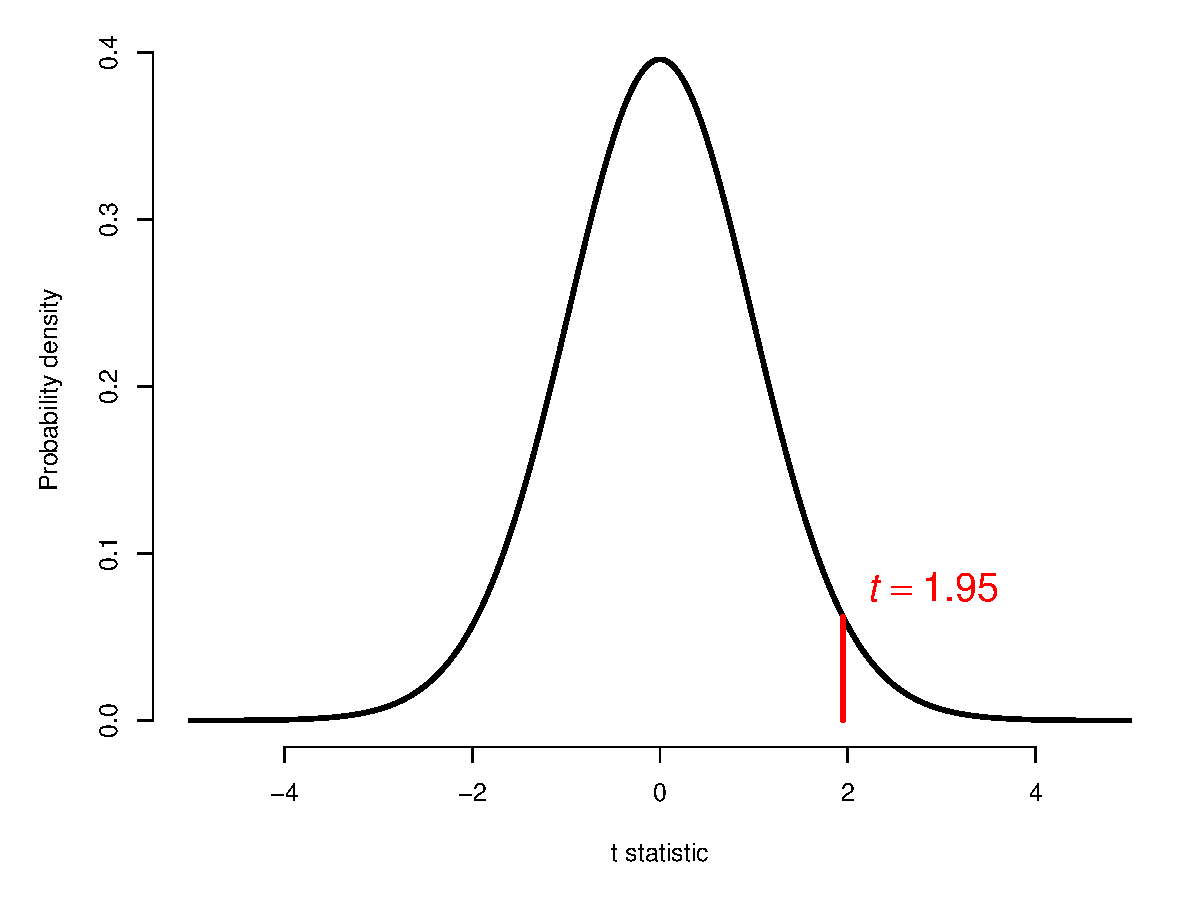
\includegraphics[keepaspectratio]{chapters/ch15_files/figure-pdf/unnamed-chunk-6-1.pdf}}

The question for the hypothesis test is: in a dataset with 31.2 DF, how
often should we observe \emph{t} values at least as large as 1.95 (i.e.,
\(\left|t\right|\ge1.95\))? That proportion is the area shaded below:

\pandocbounded{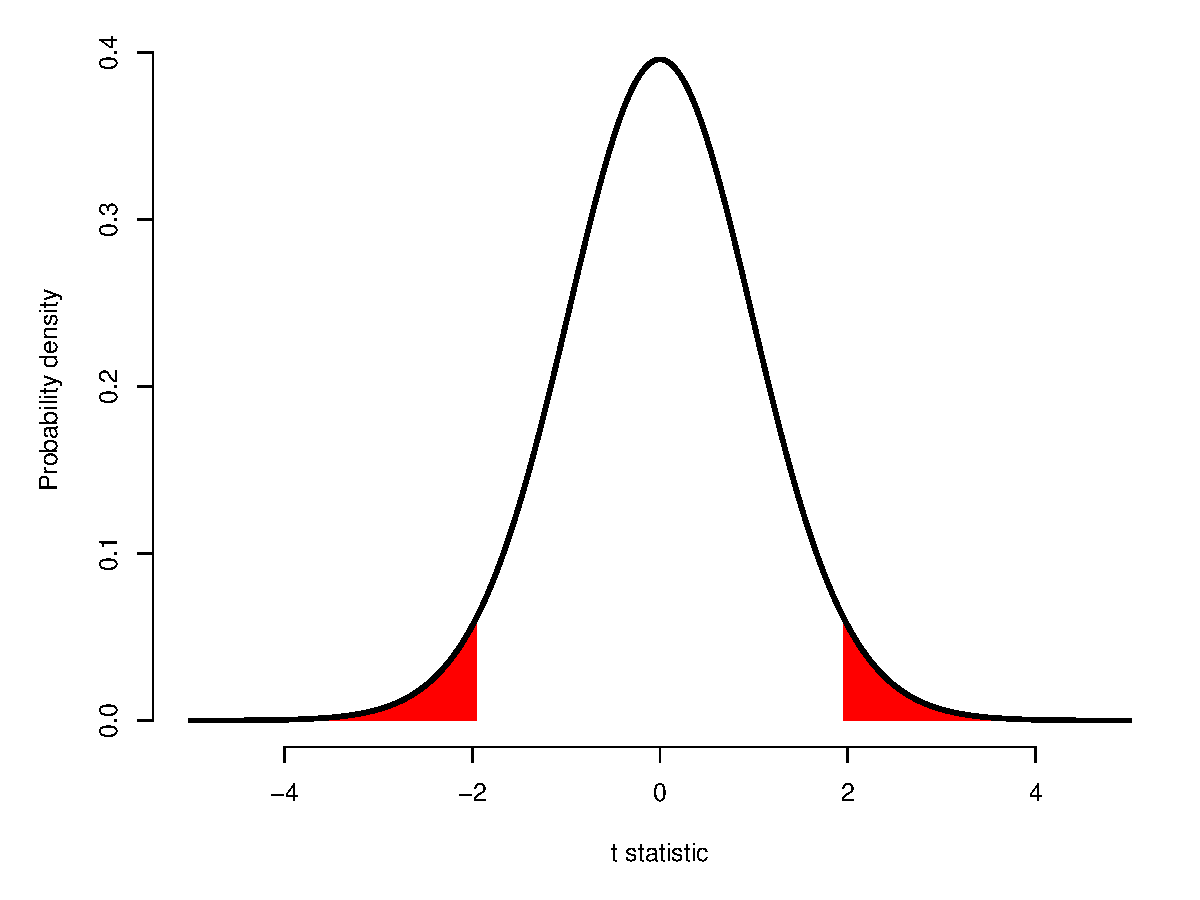
\includegraphics[keepaspectratio]{chapters/ch15_files/figure-pdf/unnamed-chunk-7-1.pdf}}

The area of the left shaded area is \texttt{pt(-1.95,\ 31.2)}, which is
\texttt{0.0301}. The distribution is symmetrical, so
\(p\left(\left|t\right|\ge1.95\right)=0.0301\times2=0.0602\). Thus, the
test was not significant (\emph{t} = 1.95, 31.2 d.f., \emph{p} = 0.06).

\textbf{Question:} Do two groups have the same underlying population
mean?

\textbf{Null hypothesis:} The true difference in means = 0. I.e.,
\(\mu_1=\mu_2\).

\textbf{Alternative hypothesis:} True difference in means is \(\neq0\).
I.e., \(\mu_1\neq\mu_2\).

\textbf{Example use case:} Barney needs to test whether tomato plants
treated with a new pesticide have a different yield (g tomato / plant)
than plants in the untreated control group.

Below is an example where we simulate some data and run a two-sample,
two-tailed test to compare the means of two groups.

\begin{Shaded}
\begin{Highlighting}[]
\CommentTok{\# simulate data}
\FunctionTok{set.seed}\NormalTok{(}\DecValTok{42}\NormalTok{)}
\NormalTok{a }\OtherTok{\textless{}{-}} \FunctionTok{rnorm}\NormalTok{(}\DecValTok{100}\NormalTok{, }\DecValTok{5}\NormalTok{, }\DecValTok{2}\NormalTok{)}
\NormalTok{b }\OtherTok{\textless{}{-}} \FunctionTok{rnorm}\NormalTok{(}\DecValTok{100}\NormalTok{, }\DecValTok{3}\NormalTok{, }\DecValTok{2}\NormalTok{)}

\CommentTok{\# example 1: difference in means}
\FunctionTok{t.test}\NormalTok{(a,b)}
\end{Highlighting}
\end{Shaded}

\begin{verbatim}

    Welch Two Sample t-test

data:  a and b
t = 8.1211, df = 194.18, p-value = 5.241e-14
alternative hypothesis: true difference in means is not equal to 0
95 percent confidence interval:
 1.696004 2.783990
sample estimates:
mean of x mean of y 
 5.065030  2.825033 
\end{verbatim}

Interpretation: The researcher should conclude that there is a
statistically significant difference between the means of groups a and
b. In a manuscript, you should report the test statistic, the DF, and
the \emph{p}-value. E.g., ``There was a significant difference in means
between group a and group b (\(t=8.121\), 194.18 d.f., \(p<0.001\)).''
Notice that values are rounded to 2 or 3 decimal places, which is
usually enough for biology. This is especially true for the
\emph{p}-value, which can be approximated by R down to infinitesimally
small values. I always round those to 0.001 or 0.0001.

A \emph{t}-test can also be performed using the \textbf{formula}
interface, which is an R programming construct for specifying a response
variable and its predictors. Notice that the formula interface here is
the same as used in \texttt{boxplot()}
(Section~\ref{sec-plot1-sing-box}) and \texttt{aggregate()}
(Section~\ref{sec-summ-agg}).

\textbf{Syntax note:} Formula syntax has the response variable on the
left, then a \texttt{\textasciitilde{}}, then the predictor or
predictors. For predictors, \texttt{a\ +\ b} means an additive model;
while \texttt{a\ *\ b} specifies an interaction. For a \emph{t}-test,
there can be only 1 predictor. If you want to test \(>1\) predictor at a
time, you need to use ANOVA instead.

Here are some common formula examples:

\begin{longtable}[]{@{}
  >{\raggedright\arraybackslash}p{(\linewidth - 2\tabcolsep) * \real{0.5000}}
  >{\raggedright\arraybackslash}p{(\linewidth - 2\tabcolsep) * \real{0.5000}}@{}}
\caption{Common R model formulas and their
meanings.}\label{tbl-model-formulas}\tabularnewline
\toprule\noalign{}
\begin{minipage}[b]{\linewidth}\raggedright
Formula
\end{minipage} & \begin{minipage}[b]{\linewidth}\raggedright
Meaning
\end{minipage} \\
\midrule\noalign{}
\endfirsthead
\toprule\noalign{}
\begin{minipage}[b]{\linewidth}\raggedright
Formula
\end{minipage} & \begin{minipage}[b]{\linewidth}\raggedright
Meaning
\end{minipage} \\
\midrule\noalign{}
\endhead
\bottomrule\noalign{}
\endlastfoot
\texttt{y\ \textasciitilde{}\ x} & \texttt{y} is modeled as a function
of \texttt{x}. \\
\texttt{y\ \textasciitilde{}\ x1\ +\ x2} & \texttt{y} is modeled as a
function of \texttt{x1} and \texttt{x2}, with their effects treated as
\textbf{additive} (i.e., no interaction between them is included). \\
\texttt{y\ \textasciitilde{}\ x1\ *\ x2} & \texttt{y} is modeled as a
function of \texttt{x1}, \texttt{x2}, and their \textbf{interaction}. An
interaction means that the effect of one predictor depends on the value
of the other predictor. This is shorthand for
\texttt{y\textasciitilde{}x1\ +\ x2\ +\ x1:x2}. \\
\texttt{y\ \textasciitilde{}\ 1} & \texttt{y} is modeled using only a
constant (the intercept), with no predictors. This is often called an
\textbf{intercept-only} or \textbf{null model}. \\
\texttt{y\ \textasciitilde{}\ 0\ +\ x} & \texttt{y} is modeled as a
function of \texttt{x}, but without an intercept (i.e., the intercept is
constrained to 0). \\
\end{longtable}

The formula interface is used in several contexts in R, including
plotting, modeling, and aggregating.

\begin{Shaded}
\begin{Highlighting}[]
\CommentTok{\# pull some data from example dataset iris}
\CommentTok{\# i.e., make a new data frame with only 2 groups}
\NormalTok{dx }\OtherTok{\textless{}{-}}\NormalTok{ iris[}\FunctionTok{which}\NormalTok{(iris}\SpecialCharTok{$}\NormalTok{Species }\SpecialCharTok{\%in\%} \FunctionTok{c}\NormalTok{(}\StringTok{"setosa"}\NormalTok{, }\StringTok{"versicolor"}\NormalTok{)),]}

\CommentTok{\# perform the test.}
\FunctionTok{t.test}\NormalTok{(Petal.Length}\SpecialCharTok{\textasciitilde{}}\NormalTok{Species, }\AttributeTok{data=}\NormalTok{dx)}
\end{Highlighting}
\end{Shaded}

\begin{verbatim}

    Welch Two Sample t-test

data:  Petal.Length by Species
t = -39.493, df = 62.14, p-value < 2.2e-16
alternative hypothesis: true difference in means between group setosa and group versicolor is not equal to 0
95 percent confidence interval:
 -2.939618 -2.656382
sample estimates:
    mean in group setosa mean in group versicolor 
                   1.462                    4.260 
\end{verbatim}

Interpretation: The researcher should conclude that there is a
statistically significant difference between the mean petal length of
\emph{Iris setosa} and \emph{Iris versicolor}.

\subsection{\texorpdfstring{Two-sample, one-tailed
\emph{t}-tests}{Two-sample, one-tailed t-tests}}\label{sec-groups-2samp-1t}

\textbf{Question:} Is the true difference in means between 2 groups
greater than, or less than, some target value \(\mu\)?

\textbf{Null hypothesis:} The true difference in means between 2 groups
is \(\mu\). I.e., \(\mu_1-\mu_2=\mu\).

\textbf{Alternative hypothesis:} The true difference in means between 2
groups is either greater than \(>\mu\) or \(<\mu\). I.e., either
\(\mu_1-\mu_2>\mu\) or \(\mu_1-\mu_2<\mu\).

\textbf{Example use case:} Betty needs to compare two stock solutions
and check that their pH differs by no more than 0.2.

The 2-sample, 1-tailed \emph{t}-test that can be used in several ways:

\begin{enumerate}
\def\labelenumi{\arabic{enumi}.}
\tightlist
\item
  Test whether the mean in one group is greater or less than the mean in
  another group.
\item
  Test whether the the mean in one group is greater or less than the
  mean in another group, and that the difference is at least some
  specified value.
\end{enumerate}

For example, if you know that the mean of group 1 must be less than the
mean in group 2, and will not even consider that the mean of group 2 is
less than that of group 1, then you could run a 2-sample 1-tailed test.

\begin{Shaded}
\begin{Highlighting}[]
\CommentTok{\# simulate data}
\FunctionTok{set.seed}\NormalTok{(}\DecValTok{789}\NormalTok{)}
\NormalTok{x1 }\OtherTok{\textless{}{-}} \FunctionTok{rnorm}\NormalTok{(}\DecValTok{20}\NormalTok{, }\DecValTok{10}\NormalTok{, }\DecValTok{1}\NormalTok{)}
\NormalTok{x2 }\OtherTok{\textless{}{-}} \FunctionTok{rnorm}\NormalTok{(}\DecValTok{20}\NormalTok{, }\DecValTok{12}\NormalTok{, }\DecValTok{1}\NormalTok{)}

\CommentTok{\# is mean(x1) \textgreater{} mean(x2)?}
\FunctionTok{t.test}\NormalTok{(x1, x2, }\AttributeTok{alternative=}\StringTok{"greater"}\NormalTok{)}
\end{Highlighting}
\end{Shaded}

\begin{verbatim}

    Welch Two Sample t-test

data:  x1 and x2
t = -8.8728, df = 37.99, p-value = 1
alternative hypothesis: true difference in means is greater than 0
95 percent confidence interval:
 -2.402592       Inf
sample estimates:
mean of x mean of y 
 9.689982 11.708940 
\end{verbatim}

\begin{Shaded}
\begin{Highlighting}[]
\CommentTok{\# is mean(x1) \textless{} mean(x2)?}
\FunctionTok{t.test}\NormalTok{(x1, x2, }\AttributeTok{alternative=}\StringTok{"less"}\NormalTok{)}
\end{Highlighting}
\end{Shaded}

\begin{verbatim}

    Welch Two Sample t-test

data:  x1 and x2
t = -8.8728, df = 37.99, p-value = 4.259e-11
alternative hypothesis: true difference in means is less than 0
95 percent confidence interval:
      -Inf -1.635323
sample estimates:
mean of x mean of y 
 9.689982 11.708940 
\end{verbatim}

\begin{Shaded}
\begin{Highlighting}[]
\CommentTok{\# is mean(x1) {-} mean(x2) at least 1?}
\FunctionTok{t.test}\NormalTok{(x1, x2, }\AttributeTok{alternative=}\StringTok{"greater"}\NormalTok{, }\AttributeTok{mu=}\DecValTok{1}\NormalTok{)}
\end{Highlighting}
\end{Shaded}

\begin{verbatim}

    Welch Two Sample t-test

data:  x1 and x2
t = -13.267, df = 37.99, p-value = 1
alternative hypothesis: true difference in means is greater than 1
95 percent confidence interval:
 -2.402592       Inf
sample estimates:
mean of x mean of y 
 9.689982 11.708940 
\end{verbatim}

\begin{Shaded}
\begin{Highlighting}[]
\CommentTok{\# is mean(x1) {-} mean(x2) at most 1?}
\FunctionTok{t.test}\NormalTok{(x1, x2, }\AttributeTok{alternative=}\StringTok{"less"}\NormalTok{, }\AttributeTok{mu=}\DecValTok{1}\NormalTok{)}
\end{Highlighting}
\end{Shaded}

\begin{verbatim}

    Welch Two Sample t-test

data:  x1 and x2
t = -13.267, df = 37.99, p-value = 3.867e-16
alternative hypothesis: true difference in means is less than 1
95 percent confidence interval:
      -Inf -1.635323
sample estimates:
mean of x mean of y 
 9.689982 11.708940 
\end{verbatim}

an uncommon variant used to test whether two groups have a difference in
means that is less than or greater than some specified value. For
example, if you produce two batches of bacteria by inoculation,
incubation, and then serial dilution, you may want to confirm that the
difference in cell count between them is less than some acceptable
value. You could use a 2-sample, 1-tailed test with the ``alternative''
hypothesis being that the difference is ``greater'' than your benchmark.

\begin{Shaded}
\begin{Highlighting}[]
\FunctionTok{set.seed}\NormalTok{(}\DecValTok{789}\NormalTok{)}
\NormalTok{x1 }\OtherTok{\textless{}{-}} \FunctionTok{rnorm}\NormalTok{(}\DecValTok{30}\NormalTok{, }\DecValTok{5}\NormalTok{, }\DecValTok{2}\NormalTok{)}
\NormalTok{x2 }\OtherTok{\textless{}{-}} \FunctionTok{rnorm}\NormalTok{(}\DecValTok{30}\NormalTok{, }\FloatTok{5.5}\NormalTok{, }\DecValTok{2}\NormalTok{)}

\CommentTok{\# is the true difference in means \textless{}1?}
\FunctionTok{t.test}\NormalTok{(x1, x2, }\AttributeTok{alternative=}\StringTok{"greater"}\NormalTok{)}
\end{Highlighting}
\end{Shaded}

\begin{verbatim}

    Welch Two Sample t-test

data:  x1 and x2
t = -2.6676, df = 50.08, p-value = 0.9949
alternative hypothesis: true difference in means is greater than 0
95 percent confidence interval:
 -2.048126       Inf
sample estimates:
mean of x mean of y 
 4.438104  5.696001 
\end{verbatim}

\subsection{Equivalence testing}\label{sec-groups-1samp-tost}

It is not possible to demonstrate statistically that a difference in
means is truly 0, or that the underlying mean of a set of data truly is
equal to a target value \(\mu\) (the converse of a one-sample,
two-tailed \emph{t}-test). With a 1-sample, 2-tailed test the best you
can do is ``fail to reject'' the null hypothesis that the mean is 0.
However, we can show that the difference is arbitrarily close to 0. This
approach is called \textbf{equivalence testing}, and one method is the
\textbf{two one-sided tests} (\textbf{TOST}) method. The method works
like this:

\begin{figure}[H]

\caption{Illustration of the two one-sided test (TOST) strategy for
establishing that a sample, or set of differences, has an underlying
mean arbitrarily close to some value \(\mu\) (\(\mu=0\) in this
example.)}

{\centering \pandocbounded{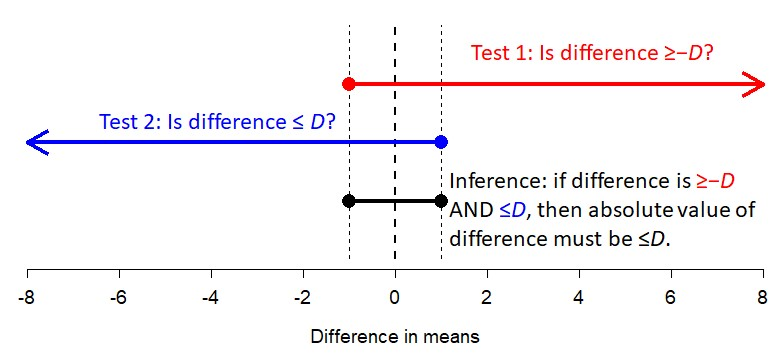
\includegraphics[keepaspectratio]{chapters/../images/review-03.jpg}}

}

\end{figure}%

Here is a worked TOST equivalence test example in R:

\begin{Shaded}
\begin{Highlighting}[]
\CommentTok{\# simulate data}
\FunctionTok{set.seed}\NormalTok{(}\DecValTok{42}\NormalTok{)}
\NormalTok{a }\OtherTok{\textless{}{-}} \FunctionTok{rnorm}\NormalTok{(}\DecValTok{100}\NormalTok{, }\DecValTok{5}\NormalTok{, }\DecValTok{1}\NormalTok{)}
\NormalTok{b }\OtherTok{\textless{}{-}} \FunctionTok{rnorm}\NormalTok{(}\DecValTok{100}\NormalTok{, }\DecValTok{5}\NormalTok{, }\DecValTok{1}\NormalTok{)}

\CommentTok{\# let target tolerance = 1}
\CommentTok{\# note that total tolerance range is 1, so}
\CommentTok{\# amount for both one{-}sided tests is 1/2==0.5}
\NormalTok{D }\OtherTok{\textless{}{-}} \FloatTok{0.5}

\CommentTok{\# test 1: is difference \textgreater{}{-}D?}
\FunctionTok{t.test}\NormalTok{(a, b, }\AttributeTok{alternative =} \StringTok{"greater"}\NormalTok{, }\AttributeTok{mu=}\SpecialCharTok{{-}}\NormalTok{D)}
\end{Highlighting}
\end{Shaded}

\begin{verbatim}

    Welch Two Sample t-test

data:  a and b
t = 4.4956, df = 194.18, p-value = 5.955e-06
alternative hypothesis: true difference in means is greater than -0.5
95 percent confidence interval:
 -0.1079329        Inf
sample estimates:
mean of x mean of y 
 5.032515  4.912516 
\end{verbatim}

\begin{Shaded}
\begin{Highlighting}[]
\CommentTok{\# test 2: is difference \textless{}D?}
\FunctionTok{t.test}\NormalTok{(a, b, }\AttributeTok{alternative =} \StringTok{"less"}\NormalTok{, }\AttributeTok{mu=}\NormalTok{D)}
\end{Highlighting}
\end{Shaded}

\begin{verbatim}

    Welch Two Sample t-test

data:  a and b
t = -2.7554, df = 194.18, p-value = 0.00321
alternative hypothesis: true difference in means is less than 0.5
95 percent confidence interval:
    -Inf 0.34793
sample estimates:
mean of x mean of y 
 5.032515  4.912516 
\end{verbatim}

Interpretation: Test 1 showed that the difference in means is \(>-0.5\).
Test 2 showed that the difference in means is \(<0.5\). So, the
difference in means is in the interval \(\left(-0.5,0.5\right)\), which
means the difference in means is at most 0.5 in either direction.

\subsection{Wilcoxon rank-sum test}\label{sec-groups-2samp-wilcoxon}

\textbf{Question:} Are values in one group consistently greater than or
less than those in another group? OR: Is the median rank in one group
different from that in another group?

\textbf{Null hypothesis:} For randomly selected values \(x\) and \(y\)
from two groups, \(p\left(x>y\right)=p\left(y>x\right)\).

\textbf{Alternative hypothesis:} For randomly selected values X and Y
from two groups, \(p\left(x>y\right)\neq p\left(y>x\right)\).

\textbf{Example use case:} Homer is interested in whether plots where
invasive plants have been removed have more squirrels than plots where
invasive plants are not removed, but does not want to model the actual
number of squirrels.

The \textbf{Mann-Whitney \emph{U} test}, also known as the
\textbf{Wilcoxon test}, is a nonparametric alternative to the two-sample
\emph{t}-test. \textbf{Nonparametric} means that the test does not make
restrictive assumptions about the distribution of the data or a test
statistic. Nonparametric tests are often based on the \textbf{ranks} of
the data: the smallest value is rank 1, the next smallest is rank 2, and
so on. Because of this, nonparametric tests allow you make statements
about how consistent a pattern is, rather than about the actual values.

This test has two common use cases:

\begin{itemize}
\item
  The researcher is only interested in whether values in one group are
  consistently larger than those in another group.
\item
  The researcher needs to perform a \emph{t}-test, but the data do not
  meet the assumptions of the \emph{t}-test.
\end{itemize}

The syntax for the Wilcoxon test is fairly similar to that of a
\emph{t}-test.

Example Wilcoxon test in R:

\begin{Shaded}
\begin{Highlighting}[]
\CommentTok{\# simulate some data:}
\FunctionTok{set.seed}\NormalTok{(}\DecValTok{123}\NormalTok{)}
\NormalTok{a }\OtherTok{\textless{}{-}} \FunctionTok{runif}\NormalTok{(}\DecValTok{20}\NormalTok{, }\DecValTok{1}\NormalTok{, }\DecValTok{6}\NormalTok{)}
\NormalTok{b }\OtherTok{\textless{}{-}} \FunctionTok{runif}\NormalTok{(}\DecValTok{20}\NormalTok{, }\DecValTok{4}\NormalTok{, }\DecValTok{9}\NormalTok{)}

\CommentTok{\# run the test}
\FunctionTok{wilcox.test}\NormalTok{(a,b)}
\end{Highlighting}
\end{Shaded}

\begin{verbatim}

    Wilcoxon rank sum exact test

data:  a and b
W = 35, p-value = 1.126e-06
alternative hypothesis: true location shift is not equal to 0
\end{verbatim}

Here is the same kind of test, but using the formula interface. You can
use the formula interface for \emph{t}-tests as well.

\begin{Shaded}
\begin{Highlighting}[]
\CommentTok{\# pull some data from example dataset iris}
\CommentTok{\# i.e., make a new data frame with only 2 groups}
\NormalTok{use.species }\OtherTok{\textless{}{-}} \FunctionTok{c}\NormalTok{(}\StringTok{"versicolor"}\NormalTok{, }\StringTok{"virginica"}\NormalTok{)}
\NormalTok{dx }\OtherTok{\textless{}{-}}\NormalTok{ iris[}\FunctionTok{which}\NormalTok{(iris}\SpecialCharTok{$}\NormalTok{Species }\SpecialCharTok{\%in\%}\NormalTok{ use.species),]}
\NormalTok{dx}\SpecialCharTok{$}\NormalTok{Species }\OtherTok{\textless{}{-}} \FunctionTok{factor}\NormalTok{(dx}\SpecialCharTok{$}\NormalTok{Species, }\AttributeTok{levels=}\NormalTok{use.species)}

\CommentTok{\# perform the test.}
\FunctionTok{wilcox.test}\NormalTok{(Petal.Length}\SpecialCharTok{\textasciitilde{}}\NormalTok{Species, }\AttributeTok{data=}\NormalTok{dx)}
\end{Highlighting}
\end{Shaded}

\begin{verbatim}

    Wilcoxon rank sum test with continuity correction

data:  Petal.Length by Species
W = 44.5, p-value < 2.2e-16
alternative hypothesis: true location shift is not equal to 0
\end{verbatim}

Interpretation: The researcher can say that values in one group are
consistently greater than values in the other group. Which way that goes
should be obvious from looking at the sample medians or a boxplot.

\begin{Shaded}
\begin{Highlighting}[]
\CommentTok{\# follow up the test with a boxplot}
\CommentTok{\# note that the formula interface is used here as well!}
\FunctionTok{boxplot}\NormalTok{(Petal.Length}\SpecialCharTok{\textasciitilde{}}\NormalTok{Species, }\AttributeTok{data=}\NormalTok{dx)}
\end{Highlighting}
\end{Shaded}

\pandocbounded{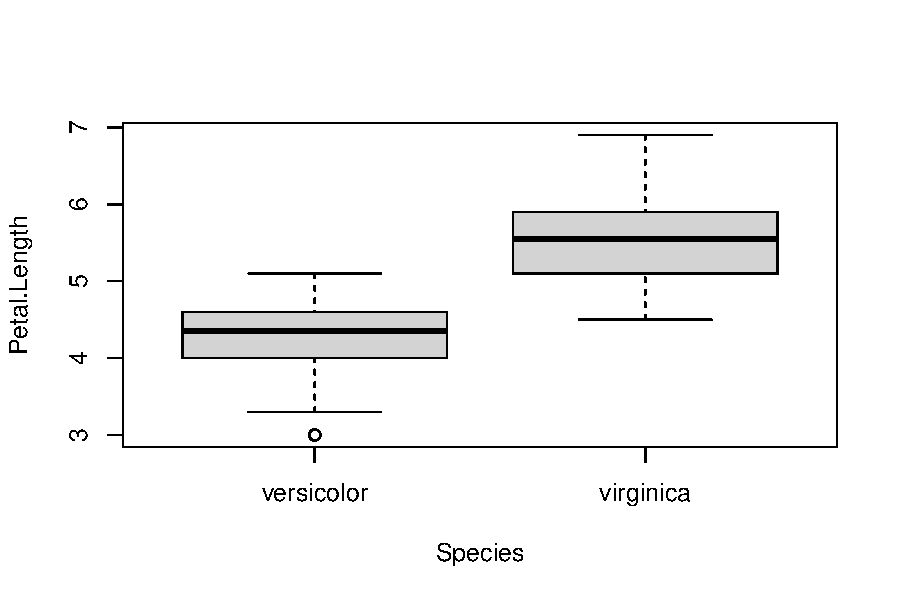
\includegraphics[keepaspectratio]{chapters/ch15_files/figure-pdf/unnamed-chunk-16-1.pdf}}

When sample sizes or effect sizes are large, the Wilcoxon test and the
\emph{t}-test will often give the same answers in terms of significance
vs. nonsignificance.

Because the \emph{t}-test tests for a difference in means, and the
Wilcoxon is its rank-based alternative, some people think that the
Wilcoxon test is a test for a difference in medians\ldots but this is
\textbf{not correct}. It's more accurate to say that the Wilcoxon test
tests for a median difference.

\section{Tests for paired data}\label{sec-groups-paired}

\subsection{\texorpdfstring{Paired
\emph{t}-test}{Paired t-test}}\label{sec-groups-paired-pt}

\textbf{Question:} Is the mean of the differences of paired observations
= 0, or different from 0?

\textbf{Null hypothesis:} Mean of pairwise differences = 0.

\textbf{Alternative hypothesis:} Mean of pairwise differences \(\neq0\).

\textbf{Example use case:} Pebbles needs to test for a mean change in
the body mass of individual mice before and after a feeding trial. Each
mouse is weighed both before and after the trial.

Many biological experiments involved \textbf{paired samples}, where a
single unit or entity was measured twice. For example, a single mouse
might be weighed before and after a feeding trial. In a \textbf{paired
\emph{t}-test}, we test whether or not the mean of differences is 0.
This is subtly different than the test for differences in means
evaluated in a two-sample test. Consequently, a paired \emph{t}-test is
tantamount to a one-sample test on the pairwise differences. Compare the
null hypotheses tested by the two-sample \emph{t}-test and paired
\emph{t}-test below:

\textbf{Two-sample \emph{t}-test:}
\(\frac{\sum_{i=1}^{n_1}x_{1,i}}{n_1}=\frac{\sum_{i=1}^{n_2}x_{2,i}}{n_2}\)

\textbf{Paired \emph{t}-test:}
\(\frac{\sum_{i=1}^{n}{x_{1,i}-x_{2,i}}}{n}=0\)

Let's simulate some data, conduct a paired \emph{t}-test, and convince
ourselves that the paired \emph{t}-test is equivalent to a one-sample
test on pairwise differences.

\begin{Shaded}
\begin{Highlighting}[]
\CommentTok{\# Example paired t{-}test in R}
\CommentTok{\# simulate data}
\FunctionTok{set.seed}\NormalTok{(}\DecValTok{42}\NormalTok{)}
\NormalTok{a }\OtherTok{\textless{}{-}} \FunctionTok{rnorm}\NormalTok{(}\DecValTok{100}\NormalTok{, }\DecValTok{5}\NormalTok{, }\DecValTok{2}\NormalTok{)}
\CommentTok{\# add pair{-}wise differences}
\NormalTok{b }\OtherTok{\textless{}{-}}\NormalTok{ a }\SpecialCharTok{+} \FunctionTok{rnorm}\NormalTok{(}\DecValTok{100}\NormalTok{, }\DecValTok{2}\NormalTok{, }\FloatTok{0.2}\NormalTok{)}
\end{Highlighting}
\end{Shaded}

Interpretation: The researcher should conclude that the mean difference
for each subject was significantly different from 0, at -1.98 with a
95\% CI of {[}-2.02, -1.95{]}.

Note that the paired \emph{t}-test gives essentially the same result as
conducting a one-sample test on the pair-wise differences.

\begin{Shaded}
\begin{Highlighting}[]
\CommentTok{\# compare to one sample t{-}test on differences:}

\NormalTok{dif }\OtherTok{\textless{}{-}}\NormalTok{ b }\SpecialCharTok{{-}}\NormalTok{ a}
\FunctionTok{t.test}\NormalTok{(dif)}
\end{Highlighting}
\end{Shaded}

\begin{verbatim}

    One Sample t-test

data:  dif
t = 109.63, df = 99, p-value < 2.2e-16
alternative hypothesis: true mean is not equal to 0
95 percent confidence interval:
 1.946622 2.018385
sample estimates:
mean of x 
 1.982503 
\end{verbatim}

\section{\texorpdfstring{\emph{t}-test
summary}{t-test summary}}\label{sec-groups-ttests}

As we have seen, the \emph{t}-test in all of its variations is a very
useful and flexible family of tests that can be applied to many
biological problems. One of the reasons that \emph{t}-tests are so
widely applicable-and why there are so many \emph{t}-tests--is that the
test statistic \emph{t} is so elegant in its construction: it represents
the quantity of interest directly in its numerator, and then the
denominator scales that quantity according to the level of uncertainty
in the data. It is thus a kind of \textbf{signal-to-noise ratio} that
predated information theory by almost 50 years.

As a review, the table below summarizes the different \emph{t}-tests and
their use cases:

\begin{longtable}[]{@{}
  >{\raggedright\arraybackslash}p{(\linewidth - 4\tabcolsep) * \real{0.3333}}
  >{\raggedright\arraybackslash}p{(\linewidth - 4\tabcolsep) * \real{0.3333}}
  >{\raggedright\arraybackslash}p{(\linewidth - 4\tabcolsep) * \real{0.3333}}@{}}
\caption{Common types of \emph{t}-tests and the hypotheses they
evaluate.}\label{tbl-t-tests}\tabularnewline
\toprule\noalign{}
\begin{minipage}[b]{\linewidth}\raggedright
Type
\end{minipage} & \begin{minipage}[b]{\linewidth}\raggedright
Use
\end{minipage} & \begin{minipage}[b]{\linewidth}\raggedright
Section
\end{minipage} \\
\midrule\noalign{}
\endfirsthead
\toprule\noalign{}
\begin{minipage}[b]{\linewidth}\raggedright
Type
\end{minipage} & \begin{minipage}[b]{\linewidth}\raggedright
Use
\end{minipage} & \begin{minipage}[b]{\linewidth}\raggedright
Section
\end{minipage} \\
\midrule\noalign{}
\endhead
\bottomrule\noalign{}
\endlastfoot
One-sample \emph{t}-test, one-tailed & Tests whether the population mean
of a single set of values is less than or greater than a specified value
\(\mu_0\). Appropriate when differences in only one direction are of
interest. & Section~\ref{sec-groups-1samp-1t} \\
One-sample \emph{t}-test, two-tailed & Tests whether the population mean
is equal to a specified value \(\mu_0\) (null hypothesis) or differs
from it (alternative hypothesis). & Section~\ref{sec-groups-1samp-2t} \\
Two-sample \emph{t}-test, two-tailed & Tests whether the population
means of two groups (\(\mu_1\) and \(\mu_2\)) differ. This can also be
thought of as testing whether the difference between the means is equal
to 0. Welch's \emph{t}-test, which does not assume equal variances,
should generally be used and is the default in R. &
Section~\ref{sec-groups-2samp-2t} \\
Two-sample \emph{t}-test, one-tailed & Tests whether the population mean
of one group (\(\mu_1\)) is less than or greater than the mean of
another group (\(\mu_2\)). Appropriate when differences in only one
direction are of interest. & Section~\ref{sec-groups-2samp-1t} \\
Paired \emph{t}-test & Tests whether the mean difference between paired
observations differs from a specified value \(D_0\), usually 0. The test
may be one- or two-tailed depending on the hypothesis. &
Section~\ref{sec-groups-paired-pt} \\
\end{longtable}

The number of ``samples'' in a \emph{t}-test refers to how many sets of
observations are being compared. There can be either 1 sample (all
observations compared to some value) or 2 samples (2 sets of
observations compared to each other).

The number of ``tails'' refers to how sides (left (negative) and/or
right (positive)) are of interest in the test statistic distribution. In
a two-tailed test, or two-sided test, an extreme test statistic could
fall in either the right or the left tail of the distribution. The
figure below shows the range of \emph{t} values which would be declared
significant for each kind of test. Notice that for a one-tailed test,
the significance region extends closer to the center, because its area
must be equal to the same \(\alpha\) as a two-tailed test.

\begin{center}
\pandocbounded{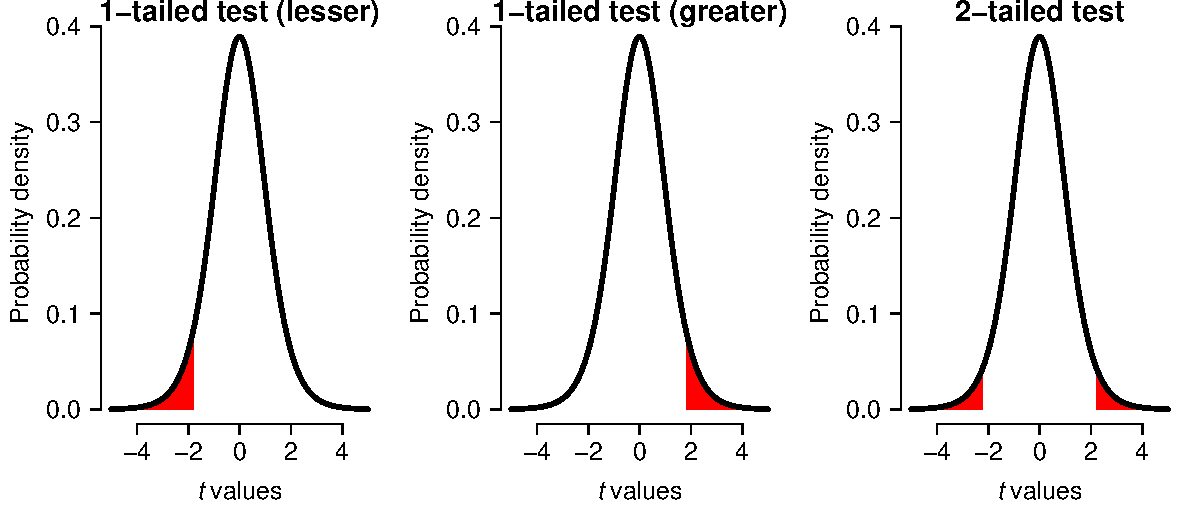
\includegraphics[keepaspectratio]{chapters/ch15_files/figure-pdf/unnamed-chunk-19-1.pdf}}
\end{center}

The \emph{t}-test is usually one of the first methods taught because its
use cases are simple, and its test statistic is pretty easy to
understand. Consider the original \emph{t} statistic introduced to the
English statistics literature by Gosset and popularized as ``Student's
\emph{t}'' by Fisher:

\[
t=\frac{\bar{x_1}-\bar{x_2}}{\sqrt{\frac{s_{x_1}^2+s_{x_2}^2}{2}}\sqrt{\frac{2}{n}}}
\]

The numerator is the quantity of interest: the difference in sample
means. It should make sense that the larger the difference in sample
means, the greater the probability that the difference will be
statistically significant. However, considering only the sample means
\(\bar{x_1}\) and \(\bar{x_2}\) is not enough. We also need to account
for variation within each sample, and for the total sample size.
Variance should \emph{decrease} \emph{t}, while sample size should
increase it. Both terms are put in the denominator so that the
difference in means is relative to them. Notice that in the denominator,
the variances \(s_{x_1}^1\) and \(s_{x_2}^1\) are in a numerator. Thus,
increasing them will decrease \emph{t}. On the other hand, the sample
size \emph{n} is in a numerator in the denominator (which is tantamount
to being in the overall numerator). Thus, increasing sample size will
increase \emph{t}.

But as elegant as Student's \emph{t} is, it has some drawbacks. It can
produce biased estimates and \emph{p}-values when the two groups have
unqual sample sizes, or unequal variances. For these reasons, a more
modern version of the \emph{t} statistic was developed by Welch in the
1940s. This is sometimes called the ``Welch's \emph{t}-test'', or less
precisely the ``Welch-Satterthwaite \emph{t}-test''. Satterthwaite's
contribution was not to the \emph{t} statistic, but rather an equation
to better calculate the degrees of freedom to use for the
test\footnote{This is why \emph{t}-tests in R often report non-integer
  degrees of freedom.}.

\[
t=\frac{\bar{x_1}-\bar{x_2}}{\sqrt{\frac{s_1}{\sqrt{n_1}}+\frac{s_2}{\sqrt{n2}}}}
\] This newer version has the same numerator, but instead of pooling the
variances and sample sizes, keeps them separate. This allows for more
flexibility when dealing with unequal sample sizes or (mildly)
heteroscedastic data.

\section{Tests for 3 or more groups}\label{sec-groups-more}

\subsection{Analysis of variance}\label{sec-groups-more-anova}

In this section, we will explore the ``test comparing group means''
sense of analysis of variance (ANOVA)
(Section~\ref{sec-review-lin-anova}). The linear model version of ANOVA
assesses significance using an \emph{F}-test. Much like \emph{t},
\emph{F} is a test statistic that summarizes a quantity of interest in a
test that can be compared to the typical strength of a pattern produced
by random noise (see Section~\ref{sec-groups-2samp-2t}\}). Whereas
\emph{t} is usually a difference in means scaled by sample size and
variance, \emph{F} compares variances. The basic idea of an \emph{F}
statistic is:

\[F=\frac{\text{explained variance}}{\text{unexplained variance}}\]

In the case of a one-way ANOVA, this translates to:

\[F=\frac{\text{between-group variability}}{\text{within-group variability}}\]

The numerator is essentially the variance in group means:

\[\sum_{i=1}^Kn_i\frac{\left(\bar{Y}_{i}-\bar{Y}\right)^2}{\left(K-1\right)}\]

where \(\bar{Y}_{i}\) is the sample mean in group \(i\), \(n_i\) is the
number of observations in group \(i\), \(\bar{Y}\) is the overall mean
of the data, and \(K\) is the number of groups.

The denominator is close to the the sum of within-group variances:

\[
\frac{
\sum_{i=1}^K\sum_{j=1}^{n_i}
\left(Y_{ij}-\bar{Y}_i\right)^2
}{
N-K
}
\]

where \(Y_{ij}\) is observation \(j\) in group \(i\) (out of \(K\)
groups), and \(N\) is the overall sample size.

The \(F\) statistic is a ratio of \emph{variance explained} to
\emph{variance not explained}. \emph{F} values follow the \emph{F}
distribution, which is defined by degrees of freedom \(d_1=K-1\) and
\(d_2=N-K\) under the null hypothesis. Practically, \emph{F} will be
large when there is more explained variance than unexplained variance,
which is unlikely if the group means are not different.

\textbf{Question:} Do the means differ between groups (with number of
groups \(\geq2\).

\textbf{Null hypothesis:} All group means are equal.

\textbf{Alternative hypothesis:} At least one group mean is different
from the others.

\textbf{Example use case:} Marge needs to test whether cucumber mass is
greater in plants grown in potting mix, sandy soil, or clayey soil.

The nature of the \emph{F} statistic belies the other meaning of ANOVA:
the partitioning of variation into its different sources. In other
words, what proportion of variation in the \emph{Y} variable does each
factor explain? How much variation is due to random chance (i.e.,
residual variation)? ANOVA in this sense can be applied to many models,
including all linear models.

The first step in a typical ANOVA is the \textbf{omnibus test}, which
assesses whether \emph{any} of the group means differ from each other.
Then, a \textbf{post-hoc test} is performed to check \emph{which} groups
differ from each other.

ANOVAs are typically described as ``X-way ANOVA'', where X is the number
of factors. For example, a test of mean stomach size in herbivorous,
carnivorous, and omnivorous mammals would be a ``one-way ANOVA'' because
it has one grouping variable, ``diet''. The three groups in the factor
diet are the \textbf{levels} of the factor.

\subsubsection{One-way ANOVA}\label{sec-groups-more-anova-1way}

When there is one explanatory \textbf{factor}, or grouping variable, the
test is called a \textbf{one-way ANOVA} regardless of how many
\textbf{levels} or groups that factor contains. Here is an example using
the built-in example dataset \texttt{iris}. There are two common ways to
fit an ANOVA in R.

\begin{Shaded}
\begin{Highlighting}[]
\CommentTok{\# method 1: lm()}
\NormalTok{mod1 }\OtherTok{\textless{}{-}} \FunctionTok{lm}\NormalTok{(Petal.Length}\SpecialCharTok{\textasciitilde{}}\NormalTok{Species, }\AttributeTok{data=}\NormalTok{iris)}

\CommentTok{\# method 2: aov()}
\NormalTok{mod2 }\OtherTok{\textless{}{-}} \FunctionTok{aov}\NormalTok{(Petal.Length}\SpecialCharTok{\textasciitilde{}}\NormalTok{Species, }\AttributeTok{data=}\NormalTok{iris)}
\end{Highlighting}
\end{Shaded}

Once the model is fit, we request the \textbf{anova table} so we can see
the contributions of each source of variation.

\begin{Shaded}
\begin{Highlighting}[]
\CommentTok{\# method 1: using lm}
\FunctionTok{anova}\NormalTok{(mod1)}
\end{Highlighting}
\end{Shaded}

\begin{verbatim}
Analysis of Variance Table

Response: Petal.Length
           Df Sum Sq Mean Sq F value    Pr(>F)    
Species     2 437.10 218.551  1180.2 < 2.2e-16 ***
Residuals 147  27.22   0.185                      
---
Signif. codes:  0 '***' 0.001 '**' 0.01 '*' 0.05 '.' 0.1 ' ' 1
\end{verbatim}

\begin{Shaded}
\begin{Highlighting}[]
\CommentTok{\# method 2: using aov}
\FunctionTok{summary}\NormalTok{(mod2)}
\end{Highlighting}
\end{Shaded}

\begin{verbatim}
             Df Sum Sq Mean Sq F value Pr(>F)    
Species       2  437.1  218.55    1180 <2e-16 ***
Residuals   147   27.2    0.19                   
---
Signif. codes:  0 '***' 0.001 '**' 0.01 '*' 0.05 '.' 0.1 ' ' 1
\end{verbatim}

No matter which method we use, the ANOVA table shows us that the factor
\texttt{Species} uses 2 degrees of freedom (variously abbreviated as DF,
Df, or d.f.) to account for 437.10 of the squared errors; the residuals
use 147 d.f. to account for 27.22 of the squared errors. The ratio of
the mean squared error per d.f. associated with each source, 218.551 /
0.185 = 1180.2, is the test statistic \emph{F}. This is used to
calculate the \emph{P}-value (much like \emph{t}, \emph{F} follows a
particular distribution defined by DF, which allows \(p(F)\) to be
calculated). We can also see that about 94.1\% of variation (437.10 /
(437.10+27.22)) is associated with species. This is the model's
coefficient of determination, or \(R^2\). The \(R^2\) tells you the
proportion of variation in \emph{Y} explained by the model.

\begin{tcolorbox}[enhanced jigsaw, arc=.35mm, bottomrule=.15mm, bottomtitle=1mm, breakable, colback=white, colbacktitle=quarto-callout-tip-color!10!white, colframe=quarto-callout-tip-color-frame, coltitle=black, left=2mm, leftrule=.75mm, opacityback=0, opacitybacktitle=0.6, rightrule=.15mm, title=\textcolor{quarto-callout-tip-color}{\faLightbulb}\hspace{0.5em}{Tip}, titlerule=0mm, toprule=.15mm, toptitle=1mm]

\textbf{Rounding errors}

R is somewhat idiosyncratic in choosing how many digits it prints, and
this can lead to confusion if values are rounded to too few decimal
places. In the ANOVA example above, the MSE for the two sources of
variation should divide to the F statistic. However,
\(218.55/0.19\neq1180\). If you look at the raw output of \texttt{mod1},
however, you that the sums of squares for Species and Residuals are
437.1028 and 27.2226, respectively. With more decimal places, you can
then recalculate
\(\left(437.1028/2\right)/\left(27.2226/147\right)=1180.161\), the
correct \(F\) ratio.

\end{tcolorbox}

Remember that the all that the omnibus test \emph{p}-value tells you is
that the means of at least one pair of species differ. To find out which
pair or pairs, we need to use a post-hoc test. My favorite is the
Tukey's honest significant difference (HSD) test because it
automatically adjusts for multiple comparisons.

\begin{Shaded}
\begin{Highlighting}[]
\CommentTok{\# method 1:}
\FunctionTok{TukeyHSD}\NormalTok{(}\FunctionTok{aov}\NormalTok{(mod1))}
\end{Highlighting}
\end{Shaded}

\begin{verbatim}
  Tukey multiple comparisons of means
    95% family-wise confidence level

Fit: aov(formula = mod1)

$Species
                      diff     lwr     upr p adj
versicolor-setosa    2.798 2.59422 3.00178     0
virginica-setosa     4.090 3.88622 4.29378     0
virginica-versicolor 1.292 1.08822 1.49578     0
\end{verbatim}

\begin{Shaded}
\begin{Highlighting}[]
\CommentTok{\# method 2:}
\FunctionTok{TukeyHSD}\NormalTok{(mod2)}
\end{Highlighting}
\end{Shaded}

\begin{verbatim}
  Tukey multiple comparisons of means
    95% family-wise confidence level

Fit: aov(formula = Petal.Length ~ Species, data = iris)

$Species
                      diff     lwr     upr p adj
versicolor-setosa    2.798 2.59422 3.00178     0
virginica-setosa     4.090 3.88622 4.29378     0
virginica-versicolor 1.292 1.08822 1.49578     0
\end{verbatim}

The Tukey output shows us that every group differs from every other,
with \emph{p\textless0.001} (here \emph{p} is rounded to 0, although it
can never be 0). The differences in group means are presented with their
\textbf{95\% confidence intervals (CI)}. For example, the difference
between the group means of versicolor and setosa is 2.798 cm, with 95\%
CI = {[}2.594, 3.002{]}. Notice that none of these CI include 0: this
suggests that a true difference of 0 between any two groups is very
unlikely. Even without examining \emph{p}-values, CI provide a useful
way to evaluate both the direction and magnitude of differences.

One of the nice things about the Tukey HSD test is that the
\emph{p}-values are automatically adjusted for \textbf{multiple
comparisons}, a phenomenon where the probability of a false positive
goes up as a \href{https://xkcd.com/882/}{researcher performs more
tests}, using a customized version of the probability distribution for
the test statistic. This controls the \textbf{family wise error rate},
or total false positive probability for this set of three related tests.

As with a \emph{t}-test, a boxplot is usually the best way to show the
results of an ANOVA.

\begin{Shaded}
\begin{Highlighting}[]
\FunctionTok{boxplot}\NormalTok{(Petal.Length}\SpecialCharTok{\textasciitilde{}}\NormalTok{Species, }\AttributeTok{data=}\NormalTok{iris, }\AttributeTok{ylim=}\FunctionTok{c}\NormalTok{(}\DecValTok{0}\NormalTok{, }\DecValTok{8}\NormalTok{))}
\end{Highlighting}
\end{Shaded}

\begin{figure}[H]

\caption{\label{fig-ttestboxplot2}Boxplot showing that petal length is
greater in \emph{Iris versicolor} than in \emph{Iris setosa}, and
greater still in \emph{Iris virginica}.}

\centering{

\pandocbounded{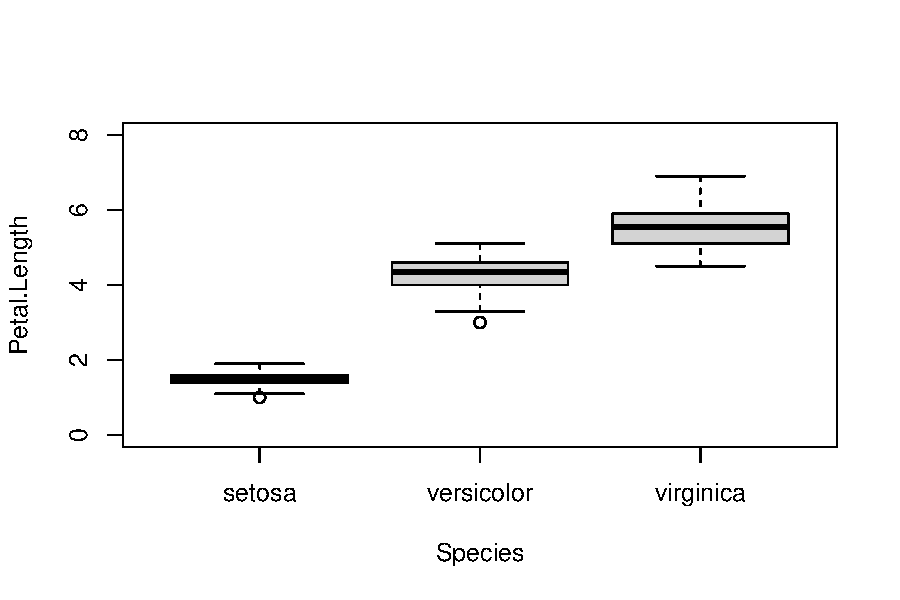
\includegraphics[keepaspectratio,alt={Boxplot showing that petal length is greater in *Iris versicolor* than in *Iris setosa*, and greater still in *Iris virginica*.}]{chapters/ch15_files/figure-pdf/fig-ttestboxplot2-1.pdf}}

}

\end{figure}%

\subsubsection{Two- or more way ANOVA}\label{sec-groups-more-anova-ways}

When there are 2 or more explanatory factors, the test is called a
\textbf{two-way ANOVA}, or \textbf{three-way ANOVA}, and so on. We can
add additional factors to an ANOVA with the \texttt{+} sign.

\begin{Shaded}
\begin{Highlighting}[]
\CommentTok{\# make a copy of iris with an extra grouping variable}
\NormalTok{iris2 }\OtherTok{\textless{}{-}}\NormalTok{ iris}
\NormalTok{iris2}\SpecialCharTok{$}\NormalTok{Flower }\OtherTok{\textless{}{-}} \FunctionTok{c}\NormalTok{(}\StringTok{"purple"}\NormalTok{, }\StringTok{"pink"}\NormalTok{)}

\CommentTok{\# fit the two{-}way ANOVA without interaction}
\NormalTok{mod3 }\OtherTok{\textless{}{-}} \FunctionTok{aov}\NormalTok{(Petal.Length}\SpecialCharTok{\textasciitilde{}}\NormalTok{Species}\SpecialCharTok{+}\NormalTok{Flower, }\AttributeTok{data=}\NormalTok{iris2)}
\FunctionTok{summary}\NormalTok{(mod3)}
\end{Highlighting}
\end{Shaded}

\begin{verbatim}
             Df Sum Sq Mean Sq  F value Pr(>F)    
Species       2  437.1  218.55 1174.229 <2e-16 ***
Flower        1    0.0    0.05    0.261   0.61    
Residuals   146   27.2    0.19                    
---
Signif. codes:  0 '***' 0.001 '**' 0.01 '*' 0.05 '.' 0.1 ' ' 1
\end{verbatim}

Adding the colors that way just repeated them until the column was full:
purple, pink, purple, pink, and so on until the new vector had length
150 (the number of rows in \texttt{iris}). This essentially distributes
the colors randomly with respect to the species and thus the petal
lengths, so it should be no surprise that flower color had no effect on
petal length (\(p=0.61\)). A Tukey test confirms the effects of species,
and the non-effect of \texttt{Flower}. Technically, you don't need to do
or report a Tukey test if the main effect is nonsignificant.

\begin{Shaded}
\begin{Highlighting}[]
\FunctionTok{TukeyHSD}\NormalTok{(mod3)}
\end{Highlighting}
\end{Shaded}

\begin{verbatim}
  Tukey multiple comparisons of means
    95% family-wise confidence level

Fit: aov(formula = Petal.Length ~ Species + Flower, data = iris2)

$Species
                      diff      lwr      upr p adj
versicolor-setosa    2.798 2.593692 3.002308     0
virginica-setosa     4.090 3.885692 4.294308     0
virginica-versicolor 1.292 1.087692 1.496308     0

$Flower
             diff        lwr       upr     p adj
purple-pink 0.036 -0.1032347 0.1752347 0.6101255
\end{verbatim}

\subsubsection{ANOVA with
interaction}\label{sec-groups-more-anova-inter}

Another important question is whether there is an \textbf{interaction}
between two variables. An interaction is a situation where one variable
changes the effect of another. To test for an interaction between two
variables, use the \texttt{*} symbol instead of the \texttt{+}. The
result \texttt{y\textasciitilde{}x1*x2} is shorthand for
\texttt{y\textasciitilde{}x1+x2+x1:x2}. The individual effects of the
variables \texttt{x1} and \texttt{x2} are called their \textbf{main
effects}. The effect of both together \texttt{x1:x2} is the
\textbf{interaction effect}. If a significant interaction effect is
detected, then the main effects should not be interpreted by themselves.

\begin{Shaded}
\begin{Highlighting}[]
\CommentTok{\# fit the two{-}way ANOVA WITH interaction}
\NormalTok{mod3 }\OtherTok{\textless{}{-}} \FunctionTok{aov}\NormalTok{(Petal.Length}\SpecialCharTok{\textasciitilde{}}\NormalTok{Species}\SpecialCharTok{*}\NormalTok{Flower, }\AttributeTok{data=}\NormalTok{iris2)}
\FunctionTok{summary}\NormalTok{(mod3)}
\end{Highlighting}
\end{Shaded}

\begin{verbatim}
                Df Sum Sq Mean Sq  F value Pr(>F)    
Species          2  437.1  218.55 1161.375 <2e-16 ***
Flower           1    0.0    0.05    0.258  0.612    
Species:Flower   2    0.1    0.04    0.201  0.818    
Residuals      144   27.1    0.19                    
---
Signif. codes:  0 '***' 0.001 '**' 0.01 '*' 0.05 '.' 0.1 ' ' 1
\end{verbatim}

The interaction is nonsignificant, so we should instead report the main
effects in the model without the interaction (\texttt{mod2}). If there
is an interaction present, then it becomes impossible to discuss the
effects of one variable without discussing the effects of the other. We
will explore interactions more in the section on ANCOVA below.

\subsubsection{Blocking designs}\label{sec-groups-more-anova-block}

\subsubsection{Repeated measures ANOVA}\label{sec-groups-more-anova-rep}

\subsubsection{Tukey's HSD post hoc
test}\label{sec-groups-more-anova-tukey}

\subsection{Kruskal-Wallis test}\label{sec-groups-more-kw}

\textbf{Question:} Are values in one or more groups consistently greater
or less than values in another group? (number of groups \(\geq3\));
essentially extends Wilcoxon test to more groups)

\textbf{Null hypothesis:} For randomly selected values \(x\) and \(y\)
from any 2 groups, \(p\left(x>y\right)=p\left(y>x\right)\).

\textbf{Alternative hypothesis:} For randomly selected values \(x\) and
\(y\) from any 2 groups, \(p\left(x>y\right)\neq p\left(y>x\right)\)

\textbf{Example use case:} Bart is studying whether tomato yields tend
to be greater in plants treated with no pesticide, pesticide A, or
pesticide B. He is not interested in predicting the actual tomato yield.

Because ANOVA is a linear model, the data used in ANOVA must meet the
\href{@sec-review-lin-assum}{assumptions of the linear model}. If the
data do not meet the assumptions, or cannot be transformed to do so,
then a nonparametric alternative to ANOVA is needed. The most common
alternative is the \textbf{Kruskal-Wallis test}. Some texts refer to
this as a ``nonparametric ANOVA'', but this is not correct because at no
point is variance actually partitioned. Like the Wilcoxon test, the
Kruskal-Wallis test is based on ranks of the data. A significant
Kruskal-Wallis test indicates that values in at least one group are
consistently greater than values in at least one other group. As with
ANOVA, a post-hoc test is needed to determine which groups differ
significantly from each other.

\textbf{Example Kruskal-Wallis test in R}

\begin{Shaded}
\begin{Highlighting}[]
\FunctionTok{kruskal.test}\NormalTok{(Petal.Length}\SpecialCharTok{\textasciitilde{}}\NormalTok{Species, }\AttributeTok{data=}\NormalTok{iris)}
\end{Highlighting}
\end{Shaded}

\begin{verbatim}

    Kruskal-Wallis rank sum test

data:  Petal.Length by Species
Kruskal-Wallis chi-squared = 130.41, df = 2, p-value < 2.2e-16
\end{verbatim}

The significant result means that petal length is consistently greater
for at least species compared to the other. This is analogous to the
omnibus ANOVA test. If we want to know which groups differ, we need a
post-hoc test. The most common option is the Dunn's test.

\begin{Shaded}
\begin{Highlighting}[]
\FunctionTok{library}\NormalTok{(dunn.test)}
\FunctionTok{dunn.test}\NormalTok{(iris}\SpecialCharTok{$}\NormalTok{Petal.Length, iris}\SpecialCharTok{$}\NormalTok{Species, }\AttributeTok{method=}\StringTok{"bonferroni"}\NormalTok{)}
\end{Highlighting}
\end{Shaded}

\begin{verbatim}
  Kruskal-Wallis rank sum test

data: x and group
Kruskal-Wallis chi-squared = 130.411, df = 2, p-value = 0

                           Comparison of x by group                            
                                 (Bonferroni)                                  
Col Mean-|
Row Mean |     setosa   versicol
---------+----------------------
versicol |  -5.862996
         |    0.0000*
         |
virginic |  -11.41838  -5.555388
         |    0.0000*    0.0000*

alpha = 0.05
Reject Ho if p <= alpha/2
\end{verbatim}

Interpretation: A posthoc Dunn's test showed that all three species
differed from each other in terms of the rank order of petal lengths.

\section{Tests with ordered factors}\label{sec-groups-ord}

Some factors can represent group membership, but still have an inherent
ordering to them. For example, soft drinks come in sizes ``small'',
``medium'', and ``large''. These are categories, but categories in
order: small \textless{} medium \textless{} large. In contrast, the
three species in the \texttt{iris} dataset have no ordering.

You may have data with a factor for age, like ``juvenile'',
``subadult'', ``adult''. These categories correspond to ages, but cannot
be treated as literal numbers of years or months. It would also be a
mistake to treat the comparison of ``juvenile vs.~subadult'' the same as
the comparison of ``juvenile vs.~adult''.

If you analyze an ordered factor, R will estimate polynomial terms of
order up to \(k-1\), where \(k\) is the number of factor levels. The
polynomial function is a way to fit different patterns across the
ordered levels. For example, a linear pattern captures a monotonic
increase or decrease across the levels. A quadratic pattern can describe
a situation where the middle of three levels has greater (or smaller)
values than the first and third levels. Let's create a toy dataset to
illustrate working with an ordered factor.

\begin{Shaded}
\begin{Highlighting}[]
\NormalTok{ages }\OtherTok{\textless{}{-}} \FunctionTok{c}\NormalTok{(}\StringTok{"juvenile"}\NormalTok{, }\StringTok{"subadult"}\NormalTok{, }\StringTok{"adult"}\NormalTok{)}
\NormalTok{dx }\OtherTok{\textless{}{-}} \FunctionTok{data.frame}\NormalTok{(}\AttributeTok{age=}\FunctionTok{rep}\NormalTok{(ages, }\AttributeTok{each=}\DecValTok{20}\NormalTok{))}
\CommentTok{\# tell R that this is an ordered factor}
\NormalTok{dx}\SpecialCharTok{$}\NormalTok{age }\OtherTok{\textless{}{-}} \FunctionTok{factor}\NormalTok{(dx}\SpecialCharTok{$}\NormalTok{age, }\AttributeTok{levels=}\NormalTok{ages, }\AttributeTok{ordered=}\ConstantTok{TRUE}\NormalTok{)}

\CommentTok{\# notice the levels statement:}
\NormalTok{dx}\SpecialCharTok{$}\NormalTok{age}
\end{Highlighting}
\end{Shaded}

\begin{verbatim}
 [1] juvenile juvenile juvenile juvenile juvenile juvenile juvenile juvenile
 [9] juvenile juvenile juvenile juvenile juvenile juvenile juvenile juvenile
[17] juvenile juvenile juvenile juvenile subadult subadult subadult subadult
[25] subadult subadult subadult subadult subadult subadult subadult subadult
[33] subadult subadult subadult subadult subadult subadult subadult subadult
[41] adult    adult    adult    adult    adult    adult    adult    adult   
[49] adult    adult    adult    adult    adult    adult    adult    adult   
[57] adult    adult    adult    adult   
Levels: juvenile < subadult < adult
\end{verbatim}

Here we use our new factor to plot and analyze french fry consumption
across age categories:

\begin{Shaded}
\begin{Highlighting}[]
\CommentTok{\# add y values}
\NormalTok{dx}\SpecialCharTok{$}\NormalTok{ff }\OtherTok{\textless{}{-}} \ConstantTok{NA}
\NormalTok{dx}\SpecialCharTok{$}\NormalTok{ff[}\FunctionTok{which}\NormalTok{(dx}\SpecialCharTok{$}\NormalTok{age}\SpecialCharTok{==}\StringTok{"juvenile"}\NormalTok{)] }\OtherTok{\textless{}{-}} \FunctionTok{rnorm}\NormalTok{(}\DecValTok{20}\NormalTok{, }\DecValTok{5}\NormalTok{, }\DecValTok{1}\NormalTok{)}
\NormalTok{dx}\SpecialCharTok{$}\NormalTok{ff[}\FunctionTok{which}\NormalTok{(dx}\SpecialCharTok{$}\NormalTok{age}\SpecialCharTok{==}\StringTok{"subadult"}\NormalTok{)] }\OtherTok{\textless{}{-}} \FunctionTok{rnorm}\NormalTok{(}\DecValTok{20}\NormalTok{, }\DecValTok{15}\NormalTok{, }\DecValTok{1}\NormalTok{)}
\NormalTok{dx}\SpecialCharTok{$}\NormalTok{ff[}\FunctionTok{which}\NormalTok{(dx}\SpecialCharTok{$}\NormalTok{age}\SpecialCharTok{==}\StringTok{"adult"}\NormalTok{)] }\OtherTok{\textless{}{-}} \FunctionTok{rnorm}\NormalTok{(}\DecValTok{20}\NormalTok{, }\DecValTok{10}\NormalTok{, }\DecValTok{1}\NormalTok{)}

\CommentTok{\# inspect the data}
\FunctionTok{boxplot}\NormalTok{(ff}\SpecialCharTok{\textasciitilde{}}\NormalTok{age, }\AttributeTok{data=}\NormalTok{dx, }\AttributeTok{ylab=}\StringTok{"French fry consumption"}\NormalTok{)}
\end{Highlighting}
\end{Shaded}

\begin{figure}[H]

\caption{\label{fig-ttestboxplot3}Boxplot showing that french fry
consumption is greatest in subadults, less in adults, and lowest in
juveniles.}

\centering{

\pandocbounded{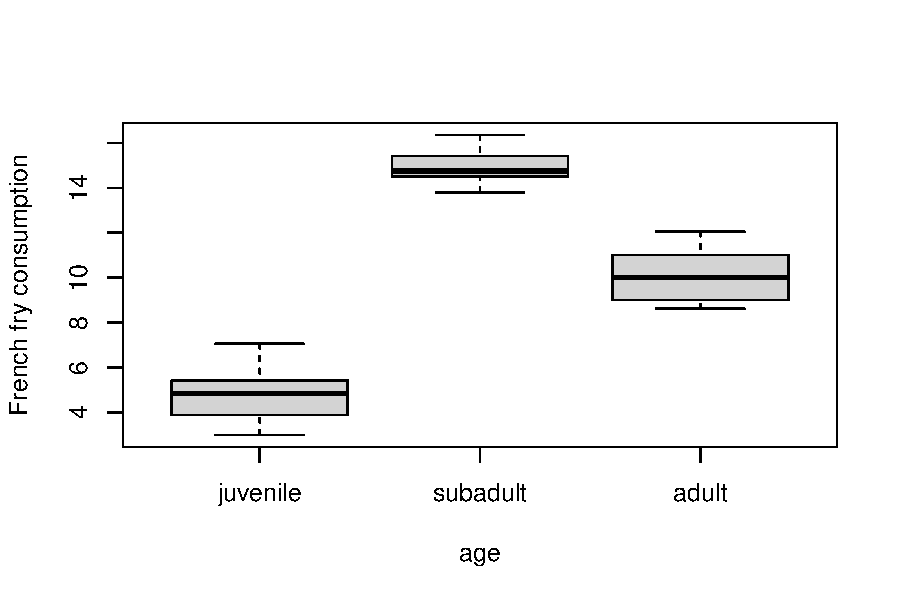
\includegraphics[keepaspectratio,alt={Boxplot showing that french fry consumption is greatest in subadults, less in adults, and lowest in juveniles.}]{chapters/ch15_files/figure-pdf/fig-ttestboxplot3-1.pdf}}

}

\end{figure}%

Now fit the model using the ordered factor \texttt{age}:

\begin{Shaded}
\begin{Highlighting}[]
\NormalTok{mod11 }\OtherTok{\textless{}{-}} \FunctionTok{aov}\NormalTok{(ff}\SpecialCharTok{\textasciitilde{}}\NormalTok{age, }\AttributeTok{data=}\NormalTok{dx)}
\FunctionTok{summary}\NormalTok{(mod11)}
\end{Highlighting}
\end{Shaded}

\begin{verbatim}
            Df Sum Sq Mean Sq F value Pr(>F)    
age          2 1008.8   504.4   526.2 <2e-16 ***
Residuals   57   54.6     1.0                   
---
Signif. codes:  0 '***' 0.001 '**' 0.01 '*' 0.05 '.' 0.1 ' ' 1
\end{verbatim}

The omnibus test shows us that \texttt{age} is significant. However,
because we have an ordered factor, we don't want something like a Tukey
test. Group means are not of interest; rather, the pattern in group
means across groups is. So, we what we want is to see which patterns
across \texttt{age} are significant.

\begin{Shaded}
\begin{Highlighting}[]
\FunctionTok{summary.lm}\NormalTok{(mod11)}
\end{Highlighting}
\end{Shaded}

\begin{verbatim}

Call:
aov(formula = ff ~ age, data = dx)

Residuals:
     Min       1Q   Median       3Q      Max 
-1.88500 -0.78190 -0.08528  0.59410  2.17546 

Coefficients:
            Estimate Std. Error t value Pr(>|t|)    
(Intercept)   9.9419     0.1264   78.66   <2e-16 ***
age.L         3.6275     0.2189   16.57   <2e-16 ***
age.Q        -6.1060     0.2189  -27.89   <2e-16 ***
---
Signif. codes:  0 '***' 0.001 '**' 0.01 '*' 0.05 '.' 0.1 ' ' 1

Residual standard error: 0.9791 on 57 degrees of freedom
Multiple R-squared:  0.9486,    Adjusted R-squared:  0.9468 
F-statistic: 526.2 on 2 and 57 DF,  p-value: < 2.2e-16
\end{verbatim}

The coefficients for \texttt{age.L} and \texttt{age.Q} are the linear
and quadratic trends, respectively. In this case, there is a positive
linear trend (\texttt{3.5113}), so \(Y\) generally increases with age
category. There is also a significant negative quadratic trend
(\texttt{-6.2328}), meaning that the relationship is curved. These
trends describe the \emph{shape} of the trend with respect to the age
categories, not literally the values of \(Y\) given \(X\) (as in a
polynomial equation), so you need to inspect the boxplot or a plot of
means.

This analysis was simple because there were only 3 levels of
\texttt{age}. When an ordered factor has many levels, you may observe
``significant'' polynomial trends that are biologically unimportant or
difficult to interpret. It is up to you as a biologist to exercise some
judgement in deciding how many terms to interpret. For example, a
quadratic pattern can be readily interpreted biologically. But what
about a quintic? Or an octic?

\chapter{Tests for continous patterns}\label{sec-lin}

\section{Correlation}\label{sec-lin-cor}

\subsection{Linear correlation}\label{sec-lin-cor-lin}

\subsection{Nonlinear correlation}\label{sec-lin-cor-non}

\section{Linear models}\label{sec-lin-lm}

\subsection{Definition}\label{sec-lin-lm-def}

\subsection{Lots of analyses are linear models in disguise (or can
be)}\label{sec-lin-lm-disguise}

\subsubsection{Ordinary linear models}\label{sec-lin-lm-disguise-lm}

\subsubsection{Polynomials}\label{sec-lin-lm-disguise-poly}

\subsubsection{Exponentials}\label{sec-lin-lm-disguise-exp}

\subsubsection{Power laws}\label{sec-lin-lm-disguise-pow}

\section{Linear regression}\label{sec-lin-reg}

\section{Multiple regression}\label{sec-lin-mult}

\section{Analysis of covariance (ANCOVA)}\label{sec-lin-ancova}

\subsection{Main effects and interaction
effects}\label{sec-lin-ancova-inter}

\chapter{Tests for contingency}\label{sec-indep}

\section{Fisher's exact test}\label{sec-indep-fisher}

\section{Chi-squared test}\label{sec-indep-chisq}

\section{G-test}\label{sec-indep-gtest}

\section{Contingency tests and odds ratios}\label{sec-indep-odds}

\part{Generalized linear models (GLM)}

Blah blah test test test.

\chapter{Introduction to generalized linear models
(GLM)}\label{sec-glm1}

A link function to the past.

\section{Prelude with linear models}\label{sec-glm1-prelude}

\section{GLM basics}\label{sec-glm1-basics}

\subsection{Overall structure}\label{sec-glm1-basics-struc}

\subsection{Response distributions}\label{sec-glm1-basics-resp}

\subsection{Linear predictors}\label{sec-glm1-basics-lp}

\subsection{Link functions}\label{sec-glm1-basics-link}

\section{Common GLMs}\label{sec-glm1-common}

\subsection{GLMs for continuous data}\label{sec-glm1-common-cont}

\subsubsection{Linear regression as a
GLM}\label{sec-glm1-common-cont-lr}

\subsubsection{GLMs for overdispersed
data}\label{sec-glm1-common-cont-over}

\subsection{GLMs for count data}\label{sec-glm1-common-count}

\subsection{GLMs for binary and proportional
data}\label{sec-glm1-common-binom}

\section{Deviance and other GLM diagnostics}\label{sec-glm1-dev}

\subsection{Deviance}\label{sec-glm1-dev-defin}

\subsection{\texorpdfstring{Pseudo-\emph{R}\^{}2 or
not?}{Pseudo-R\^{}2 or not?}}\label{sec-glm1-dev-pseudo}

\subsection{AIC and likelihood functions}\label{sec-glm1-dev-aic}

\chapter{GLM for continuous response data}\label{sec-glm2}

\section{Gaussian GLM}\label{sec-glm2-gauss}

\section{Log-normal GLM}\label{sec-glm2-lognorm}

\section{Gamma GLM}\label{sec-glm2-gamma}

\chapter{GLM for count data}\label{sec-glm3}

1! Hah ha ha

2! Hah ha ha

\section{Poisson GLM for counts}\label{sec-glm3-poisson}

\section{Negative binomial GLM for overdispersed
counts}\label{sec-glm3-negbin}

\chapter{GLM for categorical and proportional responses}\label{sec-glm4}

Even our curves have curves.

It's what's under the curve that counts.

\section{Logistic GLM for binary responses}\label{sec-glm4-logistic}

\subsection{Odds ratios}\label{sec-glm4-logistics-or}

\section{Binomial GLM for proportions}\label{sec-glm4-binom}

\section{Ordinal logistic regression}\label{sec-glm4-ord}

\part{Extensions of GLMs: nonlinear and mixed models}

Blah blah test test test.

\chapter{Nonlinear methods for biology}\label{sec-non}

Things are not always linear.

\section{Nonlinear least squares}\label{sec-non-nls}

\section{Generalized additive models (GAM)}\label{sec-non-gam}

\section{Generalized nonlinear models (GNM)}\label{sec-non-gnm}

\section{Regression trees for nonlinear patterns}\label{sec-non-cart}

\chapter{Random effects and mixed models}\label{sec-mixed}

So random.

\section{Fixed and random effects}\label{sec-mixed-effects}

\section{Linear mixed effects models (LMM)}\label{sec-mixed-lme}

\section{Generalized linear mixed effects models
(GLMM)}\label{sec-mixed-glmm}

\section{Nonlinear mixed effects models (NLME)}\label{sec-mixed-nlme}

\section{Additive mixed models (GAMM)}\label{sec-mixed-gamm}

\part{Multivariate data analysis}

Blah blah test test test.

\chapter{Introduction to multivariate data and data
analysis}\label{sec-mdata}

How far is too far?

\chapter{Dissimilarity and distance}\label{sec-diss}

How far is too far?

\section{Mantel tests}\label{mantel-tests}

\chapter{Clustering for biologists}\label{sec-clust}

Two is company, but three's a crowd.

\chapter{Ordination}\label{sec-ord}

We're all just points on a graph.

\section{Principal components analysis}\label{sec-ord-pca}

\part{Alternatives to \emph{p}-values: information-theoretic and
Bayesian methods}

Blah blah test test test.

\chapter{Multivariate hypothesis testing}\label{sec-mtest}

Anything is permuted.

\section{Comparing groups}\label{sec-mtest-group}

\subsection{MANOVA}\label{sec-mtest-group-man}

\subsection{PERMANOVA}\label{sec-mtest-group-perm}

\subsection{MRPP}\label{sec-mtest-group-mrpp}

\section{Analyzing dissimilarity}\label{sec-mtest-dis}

\subsection{Mantel tests}\label{sec-mtest-dis-mantel}

\chapter{Information theoretic model-based inference}\label{sec-it}

Ain't AIC grand?

\part{Bonus material}

Material that didn't quite fit anywhere else. Future chapters will
likely be added here.

\chapter{Introduction to Bayesian inference for
biologists}\label{sec-bayes}

Bayes bayes bayes.

\chapter{Advanced R graphics}\label{sec-plot2}

Base graphics are the best graphics.

\chapter{Classification and regression trees}\label{sec-cart}

Barking up the wrong tree

\cleardoublepage
\phantomsection
\addcontentsline{toc}{part}{Appendices}
\appendix

\chapter{Appendix A}\label{sec-appenda}

NEON small mammal data

\protect\phantomsection\label{refs}
\begin{CSLReferences}{1}{1}
\bibitem[\citeproctext]{ref-bolker2008ecological}
Bolker BM. 2008. Ecological models and data in {R}. Princeton, New
Jersey, USA: Princeton University Press.

\bibitem[\citeproctext]{ref-bolker2009}
Bolker BM, Brooks ME, Clark CJ, Geange SW, Poulsen JR, Stevens MHH,
White J-SS. 2009. Generalized linear mixed models: A practical guide for
ecology and evolution. Trends in Ecology \& Evolution 24(3):127--135.
\url{https://doi.org/10.1016/j.tree.2008.10.008}

\bibitem[\citeproctext]{ref-box1964}
Box GEP, Cox DR. 1964. An analysis of transformations. Journal of the
Royal Statistical Society: Series B (Methodological) 26(2):211--243.
\url{https://doi.org/10.1111/j.2517-6161.1964.tb00553.x}

\bibitem[\citeproctext]{ref-broman2018}
Broman KW, Woo KH. 2018. Data organization in spreadsheets. The American
Statistician 72(1):2--10.
\url{https://doi.org/10.1080/00031305.2017.1375989}

\bibitem[\citeproctext]{ref-burnham2002}
Burnham K, Anderson D. 2002. Model selection and multi-model inference:
{a} practical information-theoretic approach. New York:
Springer-{V}erlag.

\bibitem[\citeproctext]{ref-dalgaard2002}
Dalgaard P. 2002. Introductory statistics with {R}. Springer
Science+Business Media.

\bibitem[\citeproctext]{ref-dormann2013}
Dormann CF, Elith J, Bacher S, Buchmann C, Carl G, Carré G, Marquéz JRG,
Gruber B, Lafourcade B, Leitão PJ \emph{et al.} 2013. Collinearity: A
review of methods to deal with it and a simulation study evaluating
their performance. Ecography 36(1):27--46.
\url{https://doi.org/10.1111/j.1600-0587.2012.07348.x}

\bibitem[\citeproctext]{ref-gelfand2003}
Gelfand AE, Vounatsou P. 2003. Proper multivariate conditional
autoregressive models for spatial data analysis. Biostatistics
4(1):11--15. \url{https://doi.org/10.1093/biostatistics/4.1.11}

\bibitem[\citeproctext]{ref-green2019}
Green NS, Wildhaber ML, Albers JL. 2019.
\href{https://doi.org/10.1111/jai.13701}{Potential responses of the
{L}ower {M}issouri {R}iver shovelnose sturgeon (\emph{{S}caphirhynchus
platorynchus}) population to a commercial fishing ban}. Journal of
Applied Ichthyology 35(1):370--377.

\bibitem[\citeproctext]{ref-green2020}
Green NS, Wildhaber ML, Albers JL, Pettit TW, Hooper MJ. 2020.
\href{https://doi.org/10.1002/ieam.4324}{Efficient mammal biodiversity
surveys for ecological restoration monitoring}. Integrated Environmental
Assessment and Management.

\bibitem[\citeproctext]{ref-grolemund2011}
Grolemund G, Wickham H. 2011.
\href{https://www.jstatsoft.org/v40/i03/}{Dates and times made easy with
{lubridate}}. Journal of Statistical Software 40(3):1--25.

\bibitem[\citeproctext]{ref-hobbs2006}
Hobbs NT, Hilborn R. 2006.
\href{https://doi.org/10.1890/04-0645}{Alternatives to statistical
hypothesis testing in ecology: {a} guide to self teaching}. Ecological
Applications 16(1):5--19.

\bibitem[\citeproctext]{ref-hutcheon2002}
Hutcheon JM, Kirsch JAW, Jr TG. 2002. A comparative analysis of brain
size in relation to foraging ecology and phylogeny in the {C}hiroptera.
Brain, behavior and evolution 60(3):165--180.
\url{https://doi.org/10.1159/000065938}

\bibitem[\citeproctext]{ref-james2013}
James G, Witten D, Hastie T, Tibshirani R. 2013.
\href{http://faculty.marshall.usc.edu/gareth-james/ISL/}{An introduction
to statistical learning}. 7th edn. Vol. 112. Springer.

\bibitem[\citeproctext]{ref-kery2010}
Kéry M. 2010. Introduction to {W}in{BUGS} for ecologists: {B}ayesian
approach to regression, {ANOVA}, mixed models and related analyses.
Academic Press.

\bibitem[\citeproctext]{ref-kirchner2011}
Kirchner BN, Green NS, Sergeant DA, Mink JN, Wilkins KT. 2011.
\href{https://doi.org/10.1674/0003-0031-166.1.112}{Responses of small
mammals and vegetation to a prescribed burn in a tallgrass blackland
prairie}. The American Midland Naturalist 166(1):112--125.

\bibitem[\citeproctext]{ref-kuehn2012}
Kuehn I, Dormann CF. 2012.
\href{https://doi.org/10.1111/j.1365-2699.2012.02707.x}{Less than eight
(and a half) misconceptions of spatial analysis}. Journal of
Biogeography 39(5):995--998.

\bibitem[\citeproctext]{ref-lebreton1992}
Lebreton J-D, Burnham KP, Clobert J, Anderson DR. 1992.
\href{https://doi.org/10.2307/2937171}{Modeling survival and testing
biological hypotheses using marked animals: {a} unified approach with
case studies}. Ecological {M}onographs 62(1):67--118.

\bibitem[\citeproctext]{ref-legendre2012numerical}
Legendre P, Legendre L. 2012. Numerical ecology. Amsterdam: Elsevier.

\bibitem[\citeproctext]{ref-mccune2002analysis}
McCune B, Grace JB, Urban DL. 2002. Analysis of ecological communities.
MjM software design, Gleneden Beach, Oregon, USA.

\bibitem[\citeproctext]{ref-neon2025}
National Ecological Observatory Network (NEON). 2025. Small mammal box
trapping (DP1.10072.001). \url{https://doi.org/10.48443/YRH2-6058}

\bibitem[\citeproctext]{ref-penone2014}
Penone C, Davidson AD, Shoemaker KT, Di Marco M, Rondinini C, Brooks TM,
Young BE, Graham CH, Costa GC. 2014.
\href{https://doi.org/10.1111/2041-210X.12232}{Imputation of missing
data in life-history trait datasets: Which approach performs the best?}
Methods in Ecology and Evolution 5(9):961--970.

\bibitem[\citeproctext]{ref-ritz2015}
Ritz C, Baty F, Streibig JC, Gerhard D. 2015. Dose-response analysis
using {R}. PLoS ONE 10(12):e0146021.
\url{https://doi.org/10.1371/journal.pone.0146021}

\bibitem[\citeproctext]{ref-spector2008}
Spector P. 2008. Data manipulation with {R}. New York: Springer
Science+Business Media.

\bibitem[\citeproctext]{ref-warton2011}
Warton DI, Hui FKC. 2011. The arcsine is asinine: The analysis of
proportions in ecology. Ecology 92(1):3--10.
\url{https://doi.org/10.1890/10-0340.1}

\bibitem[\citeproctext]{ref-wasserstein2016}
Wasserstein RL, Lazar NA. 2016.
\href{https://doi.org/10.1080/00031305.2016.1154108}{The ASA statement
on p-values: Context, process, and purpose}. The American Statistician
70:129--133.

\bibitem[\citeproctext]{ref-wickham2014}
Wickham H. 2014. Tidy data. Journal of Statistical Software 59(10).
\url{https://doi.org/10.18637/jss.v059.i10}

\bibitem[\citeproctext]{ref-wickham2019}
Wickham H, Averick M, Bryan J, Chang W, McGowan LD, François R,
Grolemund G, Hayes A, Henry L, Hester J \emph{et al.} 2019. Welcome to
the {tidyverse}. Journal of Open Source Software 4(43):1686.
\url{https://doi.org/10.21105/joss.01686}

\bibitem[\citeproctext]{ref-wolodzko2026}
Wolodzko T. 2026.
\href{https://CRAN.R-project.org/package=extraDistr}{extraDistr:
Additional univariate and multivariate distributions}.

\bibitem[\citeproctext]{ref-zuur2007analysing}
Zuur AF, Ieno EN, Smith GM. 2007. Analysing ecological data. New York:
Springer Science+Business Media.

\bibitem[\citeproctext]{ref-zuur2009mixed}
{Zuur AF, Ieno EN, Walker NJ, Saveliev AA, Smith GM \emph{et al.}}
2009a. Mixed effects models and extensions in ecology with {R}. Vol.
574. New York: Springer.

\bibitem[\citeproctext]{ref-zuur2009}
Zuur A, Ieno EN, Meesters E. 2009b. A beginner's guide to {R}. New York:
Springer Science+Business Media.

\end{CSLReferences}




\end{document}
